\documentclass[fleqn, 12pt, a4paper, titlepage]{extarticle}
\usepackage{styles/packages}

% \usepackage{styles/styleclassic}
\usepackage{styles/style}

\usepackage{styles/general}
\usepackage{styles/titlepage}
\usepackage{styles/symbols}

\usepackage{styles/macroses/longarrows}

\rhead{\footnotesize Максимов П.А.}
\lhead{\footnotesize <<Дифференциальные уравнения>>, задачи}

\renewcommand{\drawer}{}

\begin{document}

	% \setcounter{page}{-1}
	\pagestyle{empty}
	\doctitlepage{
	\schoolfrom{ИНСТИТУТ МАТЕМАТИКИ И КОМПЬЮТЕРНЫХ ТЕХНОЛОГИЙ\\(ШКОЛА)}{Департамент математического и компьютерного моделирования}
}{
	Максимов П.А.

	\vspace{130pt}
	
	\textbf{\large Сборник задач по дисциплине \\<<Дифференциальные уравнения>>}

}{2025}


	% \vspace*{-120pt}
	\pagestyle{empty}
	\tableofcontents


	%---------------------------------------------------------------------------------------------------------------
	%===============================================================================================================
	%---------------------------------------------------------------------------------------------------------------
	
	\renewcommand{\partname}{Раздел}

	%---------------------------------------------------------------------------------------------------------------
	%===============================================================================================================
	%---------------------------------------------------------------------------------------------------------------

	\newpart{Обыкновенные дифференциальные уравнения первого порядка разрешенные относительно производной.}
	\pagestyle{fancy}

		%-----------------------------------------------------------------------------------------------------------
		%===========================================================================================================
		%-----------------------------------------------------------------------------------------------------------

		\section{Уравнения с разделяющимися переменными}

	Рассмотрим уравнения следующего вида:
	\[ y' = f \pares{x, y}, \]
	где функция $f\pares{x, y}$ представляет собой произведение двух функций разных переменных:
	\[ f\pares{x, y} = P \pares{x} \cdot Q \pares{y}. \]
	Такие уравнения называются уравнениями с разделяющимися переменными. Метод решения заключается в том, чтобы разделить переменные по разные стороны от знака равенства, учитывая, что $y' = \difft{y}{x}$:
	\[ \difft{y}{x} = P \pares{x} \cdot Q \pares{y}. \]
	Разделим данное уравнение на $Q \pares{y}$, и умножим на $dx$:
	\[ \frac{dy}{Q \pares{y}} = P \pares{x} ~ dx. \]
	Левая часть, как и правая -- выражения, зависимые каждая только от одной переменной. Такое уравнение носит название уравнения с разделенными переменными. Соответственно, обе части данного равенства можно проинтегрировать:
	\[ \int \frac{dy}{Q \pares{y}} = \int P \pares{x} ~ dx. \]
	Интегрируя, получим:
	\[ \varphi \pares{y} = \psi \pares{x} + C, \]
	где $\difft{}{y} \varphi \pares{y} = \dfrac{1}{Q \pares{y}}$, и $\difft{}{x} \psi \pares{x} = P \pares{x}$. Полученное выражение является решением исходного уравнения с разделяющимися переменными. Общий вид уравнений с разделяющимися переменными можно представить следующим образом:
	\[ M_1 \pares{x} \cdot N_1 \pares{y} ~ dx = M_2 \pares{x} \cdot N_2 \pares{y} ~ dy. \]
	Разделяя данное уравнение на функцию $N_1 \pares{y} \cdot M_2 \pares{x}$, получим уравнение с разделенными переменными, для построения решения которого необходимо будет проинтегрировать обе части.

	Начальным условием для дифференциального уравнения называется выражение вида:
	\[ y \pares{x_0} = y_0. \]
	Пара дифференциальное уравнение и начальное условие называется задачей Коши. Решением задачи Коши является частное решение исходного уравнения, удовлетворяющее начальному условию.

	\subsection{Примеры}

		Рассмотрим следующий пример:
		\[ y' \cos^2{x} = \tan{y} + \cot{y}, ~ y\pares{0} = \frac{\pi}{2}. \]
		Для начала построим общее решение уравнения. Само уравнение имеет следующий вид:
		\[ M_1 \pares{x} y' = N_2 \pares{y} \]
		Здесь $M_1 \pares{x} = \cos^2{x}$, $N_1 \pares{y} = 1$, $M_2 \pares{x} = 1$ и $N_2 \pares{y} = \tan{y} + \cot{y}$.
		Разделим все уравнение на произведение $M_1 \pares{x} \cdot N_2 \pares{y}$, и домножим на $dx$, учитывая, что $y' = \difft{y}{x}$:
		\[ \frac{dy}{\tan{y} + \cot{y}} = \frac{dx}{\cos^2{x}}. \]
		И проинтегрируем обе части. Интеграл в правой части -- табличный:
		\[ \int \frac{dx}{\cos^2{x}} = \tan{x} + C_1, \]
		в то время как в левой части мы для начала упростим выражение:
		\[ \frac{1}{\tan{y} + \cot{y}} = \frac{\sin{y} \cdot \cos{y}}{\sin^2{y} + \cos^2{y}} = \sin{y} \cdot \cos{y}. \]
		Тогда интеграл в левой части имеет следующий вид:
		\[ \int \sin{y} \cdot \cos{y} ~ dy = \frac{1}{2} \sin^2{y} + C_2. \]
		Запишем решение в общем виде:
		\[ \frac{1}{2} \sin^2{y} + C_2 = \tan{x} + C_1. \]
		Упростим данную запись, домножив на $2$ и переобозначив $C_1 - C_2 = \dfrac{C}{2}$:
		\[ \sin^2{y} = 2 \tan{x} + C, \]
		что является общим решением рассматриваемого уравнения.
		Теперь построим решение задачи Коши -- найдем значение $C$, для которого данное решение будет удовлетворять начальному условию. Подставим значения $x_0 = 0$ и $y_0 = \dfrac{\pi}{2}$ в общее решение:
		\[ \sin^2{\frac{\pi}{2}} = 2 \tan{0} + C \implies 1 = 0 + C \implies C = 1. \]
		Тогда решение задачи Коши имеет следующий вид:
		\[ \sin^2{y} = 2 \tan{x} + 1. \]
	
	\pagebreak

		\subsection{Задачи}
	
	Для следующих уравнений построить общее решение:
	% \begin{multicols}{2}
	% 	\begin{enumtasks}


	% 	\end{enumtasks}
	% \end{multicols}
		\pagebreak

		%-----------------------------------------------------------------------------------------------------------
		%===========================================================================================================
		%-----------------------------------------------------------------------------------------------------------

		\section{Однородные уравнения}
	
	Рассматривать будем уравнения следующего вида:
	\[ F \pares{x, y, y'} = 0. \]
	Положим, что функция $F$ может быть представлена в следующем виде:
	\[ F \pares{x, y, y'} = G \bpares{x, v\pares{x, y}, v'\pares{x, y}}, \]
	где $v \pares{x, y}$ -- некоторая известная сложная функция, $v' \pares{x, y}$ -- ее производная. С помощью замены $u = v \pares{x, y}$, где $u$ -- новая искомая функция, уравнение примет более упрощенный вид:
	\[ G \pares{x, u, u'} = 0. \]

	Теперь введем понятие однородной функции. Рассмотрим некоторую произвольную функцию многих переменных:
	\[ F\pares{x_1, x_2, \dots, x_n}. \]
	Такая функция будет однородной, если справедливо следующее соотношение:
	\[ F\pares{k \cdot x_1, k \cdot x_2, \dots, k \cdot x_n} = k^m \cdot F\pares{x_1, x_2, \dots, x_n}. \]
	То есть, для однородных функций справедливо следующее утверждение: если домножить каждый аргумент функции на некоторый множитель $k$, то его возможно вынести как множитель из самой функции с некоторой степенью $m$. Здесь $k$, $m$ -- вещественные числа.

	Однородной заменой считается замена вида $y = ux$, где $u$ -- новая искомая функция, зависимая от переменной $x$. Уравнения, содержащие такую замену, называются однородными уравнениями. С помощью такой замены уравнение можно свести к более простому виду, к примеру -- уравнению с разделяющимися переменными.

	Уравнения, приводящиеся к однородным имеют следующий вид:
	\[ y' = \frac{a_1 x + b_1 y + c_1}{a_2 x + b_2 y + c_2}, \quad a_i, b_i, c_i ~ - ~ \const ~ \forall i = \overline{1, 2}. \]
	Метод их решения зависит от значений $a_i, b_i, c_i$. Стоит обратить внимание, что числитель и знаменатель представляют собой выражения для уравнения прямых. Обозначим их как $l_i: a_i x + b_i y + c_i = 0$. Рассмотрим два случая:

	\begin{enumerate}
		\item Если $l_1 \parallel l_2$:

			В таком случае $a_1 = k \cdot a_2$ и $b_1 = k \cdot b_2$, где $k$ -- коэффициент масштабирования. Такое уравнение можно свести к уравнению с разделяющимися переменными с помощью замены $u = a_i x + b_i y + d$, где $i$ выбирается произвольно из значений $\overline{1, 2}$, а $d$ -- любое удобное число для подстановки.

		\item Если $l_1 \nparallel l_2$:

			В таком случае уравнение можно свести к однородному с помощью параллельного переноса всего уравнения в точку пересечения прямых $\pares{x_0, y_0}$:
			\[ \left\lbrace \begin{split} u = x - x_0 \\ v = y - y_0 \end{split} \right. \]
			Здесь $u$ -- новый аргумент, $v$ -- новая функция, зависимая от переменной $u$. Тогда:
			\[ \difft{y}{x} = \difft{v}{u} = v'_u. \]
			После такой замены, уравнение примет вид:
			\[ v'_u = \frac{a_1 u + b_1 v}{a_2 u + b_2 v}, \]
			которое можно свести к уравнению с разделяющимися переменными с помощью замены $v = w \cdot u$, где $w$ -- новая искомая функция, зависимая от $u$.

	\end{enumerate}

	Обобщенные однородные уравнения -- уравнения, замена для которых строится в виде $y = u \cdot x^m$, где $u$ -- новая функция, зависимая от переменной $x$, а $m$ -- показатель однородности. Определить его можно путем подстановки замены в уравнение. В случае, если уравнение имеет вид суммы степенных выражений:
	\[ \sum_{k \ge 0}^n a_k \cdot x^{p_k} \cdot y^{q_k} \cdot y'^{r_k} = 0, \quad a_k, p_k, q_k, r_k ~ - ~ \const ~ \forall k, \]
	то коэффициент однородности можно найти с помощью соответствующего характеристического уравнения. Оно строится по следующим правилам:
	\begin{itemize}
		\item Операции сложения, вычитания и равенства заменяются на равенства;
		\item Операция умножения заменяется на сложение, деление на вычитание;
		\item Каждый $x^p$ заменяется на $p$;
		\item Каждый $y^q$ заменяется на $m \cdot q$, где $m$ -- показатель однородности, на момент составления его значение неизвестно;
		\item Каждый $y'^{r}$ заменяется на $(m - 1) \cdot r$.
	\end{itemize}
	Если из соответствующей системы удается найти значение $m$, в таком случае можно воспользоваться заменой $y = u \cdot x^m$, или $y = u^m$, где $u$ -- новая искомая функция, зависимая от переменной $x$.

	\subsection{Примеры}

		\begin{enumerate}
			\item Рассмотрим следующий пример:
				\[ xy' = \tan{xy} - y. \]
				Стоит обратить внимание на то, что внутри функции $\tan$ находится сложная функция. Заменим ее на новую переменную:
				\[ u = xy, ~ u' = xy' + y, ~ u = u(x), ~ y = y(x). \]
				Тогда уравнение принимает следующий вид:
				\[ u' = \tan{u}. \]
				Это уравнение с разделяющимися переменными, и имеет следущее решение:
				\[ \sin{u} = C \cdot e^{x}. \]
				Вернемся к исходным переменным:
				\[ \sin{xy} = C \cdot e^{x}, \]
				что является общим решением данного уравнения.

			\item Рассмотрим другой пример:
				\[ y' = \frac{1 + x + 2y}{3 + 2x + 4y}. \]
				Как можно видеть, прямые, полученные из числителя и знаменателя -- параллельны. Такой вывод можно получить, построив определитель из коэффициентов при $x$ и $y$ в уравнениях:
				\[ \begin{vmatrix} 1 & 2 \\ 2 & 4 \end{vmatrix} = 0. \]
				Тогда положим следующую замену:
				\[ u = 1 + x + 2y, ~ u' = 1 + 2y' \implies y' = \frac{u' - 1}{2}, ~ u = u(x), ~ y = y(x). \]
				Подставим в уравнение, получим:
				\[ \frac{u' - 1}{2} = \frac{u}{2u + 1}. \]
				Упростим выражение:
				\[ u' = \frac{4u + 1}{2u + 1}. \]
				Полученное уравнение является уравнением с разделяющимися переменными. Разделим:
				\[ \frac{2u + 1}{4u + 1} ~ du = dx. \]
				Переменные разделены -- проинтегрируем:
				\[ \frac{1}{2} u + \frac{1}{8} \ln \abs{4u + 1} = x + C. \]
				Упростим выражение:
				\[ 4u + \ln\abs{4u + 1} = 8x + C \implies \pares{4u + 1} \cdot e^{4u} = C \cdot e^{8x}. \]
				Вернемся к исходной замене $u = 1 + x + 2y$:
				\[ \pares{4x + 8y + 5} \cdot e^{4x + 8y + 4} = C \cdot e^{8x}. \]
				Упростив, получим:
				\[ \pares{4x + 8y + 5} \cdot e^{8y - 4x + 4} = C, \]
				что является общим решением исходного уравнения.
			
			\item Рассмотрим еще один пример:
				\[ \pares{2x - y + 4} \cdot y' = x - 2y + 5. \]
				Сведем его к классическому виду:
				\[ y' = \frac{x - 2y + 5}{2x - y + 4}. \]
				Проверим, являются ли соответствующие прямые параллельными:
				\[ \begin{vmatrix} 1 & -2 \\ 2 & -1 \end{vmatrix} = 3 \neq 0. \]
				Прямые не являются параллельными, соответственно, найдем их точку пересечения:
				\[ \left\lbrace \begin{split} x - 2y &= -5 \\ 2x - y &= -4 \end{split} \right. \implies \left\lbrace \begin{split} x_0 &= -1 \\ y_0 &= 2 \end{split} \right. \]
				Теперь введем замену в уравнение:
				\[ \left\lbrace \begin{split} u &= x + 1 \\ v &= y - 2 \end{split} \right. \implies \left\lbrace \begin{split} x &= u - 1 \\ y &= v + 2 \end{split} \right. \implies y' = v'_u. \]
				Подставим замену в уравнение:
				\[ v'_u = \frac{(u - 1) - 2(v + 2) + 5}{2 (u - 1) - (v + 2) + 4} \implies v'_u = \frac{u - 2v}{2u - v}. \]
				Получили однородное уравнение. Сделаем замену:
				\[ v = u \cdot w, ~ v'_u = u \cdot w'_u + w, ~ w = w(u). \]
				Подставим:
				\[ uw'_u + w = \frac{u - 2uw}{2u - uw} \implies uw'_u = \frac{1 - 2w}{2 - w} - w \]
				Упростим:
				\[ uw'_u = \frac{1 - 4w + w^2}{2 - w}. \]
				Разделим переменные:
				\[ \frac{2 - w}{w^2 - 4w + 1} ~ dw = \frac{du}{u}. \]
				Интегрируя, получаем:
				\[ \ln\abs{w^2 - 4w + 1} = C - 2 \ln{u}. \]
				Упростим:
				\[ w^2 - 4w + 1 = \frac{C}{u^2}. \]
				Теперь вернемся к исходной замене, домножив на $u^2$:
				\[ \pares{y - 2}^2 - 4 \pares{y - 2} \pares{x + 1} + \pares{x + 1}^2 = C. \]
				Раскроем скобки, перенесем все свободные постоянные в $C$:
				\[ x^2 - 4xy + y^2 + 10x - 8 y = C. \]
				Полученное выражение является общим решением исходного уравнения.

			\item Рассмотрим последнее уравнение:
				\[ y' - \frac{y}{x} = y^2 + \recip{x^2}. \]
				Данное выражение представляет собой сумму степенных выражений. Попробуем найти коэффициент однородности. Для этого составим соответствующее характеристическое уравнение:
				\[ m - 1 = m - 1 = 2m = -2. \]
				Из данной системы следует, что $m = -1$.
				Тогда замена:
				\[ y = ux^{-1} \implies u = xy, ~ u' = xy' + y \implies y' = \frac{u'}{x} - \frac{u}{x^2}, ~ u = u(x), ~ y = y(x). \]
				Подставим замену в уравнение:
				\[ \frac{u'}{x} - \frac{u}{x^2} - \frac{u}{x^2} = \frac{u^2}{x^2} + \recip{x^2}. \]
				Упростим:
				\[ xu' = u^2 + 2u + 1. \]
				Получили уравнение с разделяющимися переменными. Его решение:
				\[ \recip{u + 1} = C - \ln{x}. \]
				Возвращаясь к исходным переменным:
				\[ xy + 1 = \recip{C - \ln{x}}. \]
				Таким образом получено общее решение исходного уравнения.
				
		\end{enumerate}

		\subsection{Задачи}
	
	Для следующих уравнений построить общее решение:
	\begin{multicols}{3}
		\begin{enumtasks}

			\label{firstorder:homogeneous}
			\item \( y' = x^4 + \frac{4 y}{x} \) 													% y = x^5 + Cx^4
			\item \( \pares{x + y} \cdot y' = x - y \)												% y^2 + 2xy = C + x^2
			\item \( x^2 y' = y^2 + 2xy \)															% xy + x^2 = Cy
			\item \( xy' = y + x^2 \cos{x} \) 														% \frac{y}{x} = \sin{x} + C
			\item \( xy - x^2y' = xyy' - y^2 \) 													% \frac{x}{y} + \ln{\frac{x}{y}} = C
			\item \( 2x^2 y y' + xy^2 = x - 1 \) 													% xy^2 = x - \ln{x} + C
			\item \( xy' = y - 2x^2 \cosec{\frac{y}{x}} \) 											% \cos{\frac{y}{x}} = 2x + C
			\item \( x^4 y' - 2x^3 y = y^2 \) 														% \frac{x^2}{y} = \frac{1}{x} + C
			\item \( xy' - 3y + 2x^5 = 0 \) 														% \frac{y}{x^3} + x^2 = C
			\item \( 3xy' + 3y = 2x \cos^2{xy} \) 													% 3 \tan{xy} = x^2 + C
			\item \( xy' e^{xy} = e^{-x} - ye^{xy} \)												% e^{xy} + e^{-x} = C
			\item \( y^3 + xy^2 y' + 3y = 3xy' \) 													% xy + \frac{3x}{y} = C
			\item \( y' = - \frac{y + 2}{x + 6y - 3} \) 											% xy + 2x + 3y^2 - 3y = C
			\item \( xy' - 3y = 3x^4 y^2 y' - 2x^5 \) 												% x^2 - y^3 + \frac{y}{x^3} = C
 			\item \( xy' + 2\tan{y} = 3x \sec{y} \)													% x^2 \sin{y} - x^3 = C
			
		\end{enumtasks}
	\end{multicols}

	\begin{multicols}{2}
		\begin{enumtasks}
			\label{firstorder:homogeneous2}
			\item \( 16y^3 y' = 2x + 5y^2 + 10 xyy' \)												% x^2 + 5xy^2 - 4y^4 = C
			\item \( 3x^2 y' + 3xy = x - 1 + x\ln{x} \) 											% 3xy + \pares{1 - x} \cdot \ln{x} = C
			\item \( xy^2 y' + x^2 y = x^3y' + 2x^3 y^2 + y^3 \) 									% x^2 + y^2 - x^3 y = Cxy
			\item \( y' = \frac{9x - 5y + 9}{5x - 3y + 1} \) 										% 10xy - 3y^2 + 2y - 9x^2 - 18x = C
			\item \( y' = \frac{x + 2y}{2x - y} \)													% \ln\pares{x^2 + y^2} - 4 \arctan{\frac{y}{x}} = C
			\item \( y' =  \frac{3x - y + 1}{x + 9y + 4} \)											% 2xy + 9y^2 + 8y = 3x^2 + 2x + C
			\item \( \pares{x - 3y} \cdot y' = x - y - y' + 4 \) 									% x^2 - 2xy + 4x + 3y^2 - 2y = C
			\item \( xy' + 2x + y + 4 = \pares{y + 1} \cdot y' \) 									% \pares{y - x + 1}^2 = x^2 + 10x + C
			\item \( 4y' \cdot \pares{2x + y + 3} = 4y - x - 33 \)									% \ln\pares{2y + x - 9} = \frac{3x + 15}{2y + x - 9} + C
			\item \( 3x^5 y + xy^2 y' = x^6 y' + 2y^3 \) 											% x^5 + y^2 = C x^2 y
			\item \( \pares{1 - 3x} \cdot y' = 9x + 5y - 7 \)										% \pares{45x + 40y - 47}^{3} \cdot \pares{3x - 1}^{5} = C
			\item \( y' =  \frac{9x + 7y + 44}{x - y - 4} \)										% \ln\pares{y + 3x + 8} + \frac{ 4x + 4 }{y + 3x + 8} = C
			\item \( 2x^3 y' + x^4 = 4x^2 y + y^2 \) 												% \frac{y - x^2}{y + x^2} = Cx
			\item \( x^4 y' + 3x^3 y = \ln{x} + 1 \) 												% x^3 y = x \ln{x} + C
			\item \( y' =  \frac{2x - 9y + 30}{9x - 16y + 37} \)									% \pares{8y - x - 29} \cdot \pares{y - x - 1} = C
			\item \( 2x + 4y + 2xy' + 4yy' + 2y' + 1 = 0 \) 										% 2x + 2y + \ln\pares{x + 2y} = C
			\item \( y' = \frac{2xy - 7y^2 + xy^3}{2x^2 - 7xy} \)									% \frac{x^2}{y^2} - \frac{7x}{y} + \ln{x} = C
			\item \( x^5 y' = 2x^4 y + y^2 \cos^2{\frac{x^2}{y}} \)									% 2 \tan{\frac{x^2}{y}} = \frac{1}{x^2} + C
			\item \( y' = \frac{6x - y + 9}{6x - y - 9} \)											% \pares{30x - 5y - 63}^{18} = C \cdot e^{5\pares{y - x}}
			\item \( y' \cos{ye^{x}} = 1 - y \cos{ye^{x}} \)										% \sin{ye^{x}} - e^{x} = C
			\item \( \pares{6x + 10} \cdot y' + \pares{5y + 3} = 2yy' \)							% \pares{33x - 6y + 58}^{5} \cdot \pares{5y + 3}^{6} = C
			\item \( \pares{7x + 9y - 3} \cdot y' = 7x + 9y + 1 \) 									% 4y - \ln\pares{28x + 36y - 3} = 4x + C
 			\item \( 2xyy' + y^2 \pares{x + 1} = 2e^x \)											% xy^2 e^{x} = e^{2x} + C
			\item \( \pares{x + 14} \cdot y' + 42 = 5x - y \cdot \pares{1 - 3y'} \)					% \pares{y - x + 14} \cdot \pares{3y + 5x - 14} = C
			\item \( y' = 2\sqrt{x + y} \cdot \pares{y' + 1} \cdot \cos{\pares{x + y}} - 1 \)		% \sqrt{x + y} - \sin{\pares{x + y}} = C
		
		\end{enumtasks}
	\end{multicols}

	Найти решение следующих уравнений, удолвлетворяющих начальным условиям:

	\begin{enumtasks}

		\label{firstorder:homogeneous_cauchy}
		\item \( xy' = y + \frac{x^3}{y}, ~ y(1) = 2 \)												% y^2 = x^2 \pares{x + 1}
		\item \( y' = - \frac{x + 4y - 4}{7y + 4x - 7}, ~ y(1) = 1 \)								% 8xy + 7y^2 - 14y + x^2 - 8x + 6 = 0
		\item \( xy' = y \cdot \pares{1 - 2x^2 y}, ~ y(-1) = 3 \) 									% \pares{2x^3 + 1} \cdot y = 3x
		\item \( xy' = y + 3x^4 \sec{\frac{y}{x}}, ~ y(2) = \pi \)									% \sin{\frac{y}{x}} = x^3 - 7
		\item \( \pares{9x - 13y - 37} y' = 5x - 9y - 33, ~ y(-7) = -5 \)							% \pares{13y - 5x + 61} \cdot \pares{y - x + 1} = 5
		\item \( y' = \frac{x^5 - x^2 y}{x^3 + y} + \frac{2y}{x}, ~ y(1) = -2 \)					% x^6 = 2x^5 y + y^2 + x^4
		\item \( xy' = y + 2xy^2, ~ y(1) = 1 \)														% x = y \cdot \pares{2 - x^2}
		\item \( x^2y' + xy = \cot{xy}, y(1) = \pi \) 												% \cos{xy} + x = 0
		\item \( xy' e^{x} + ye^{x} = e^{xy} \cdot \pares{e^{2x} - 2}, ~ y(\ln{2}) = 0 \)			% e^{-xy} = 4 - 2e^{-x} - e^{x}
		\item \( \pares{7y + 9x - 84} \cdot y' + 7x + 5y = 64, ~ y(1) = 10 \)						% 7 \pares{y + x - 10}\ln\pares{y + x - 10} = 2 \pares{x - 1}

	\end{enumtasks}

		\pagebreak

		%-----------------------------------------------------------------------------------------------------------
		%===========================================================================================================
		%-----------------------------------------------------------------------------------------------------------

		\section{Линейные уравнения}

	Рассматривать будем уравнения следующего вида:
	\[ a_0(x) \cdot y' + a_1(x) \cdot y = f(x). \]
	Уравнения, содержащие искомую функцию с ее производными в виде линейной комбинации с некоторыми известными функциями независимой переменной называются линейными уравнениями.

	Для линейных уравнений характерно свойство линейности для решений. Если известно $n$ частных решений $y_i(x)$ линейного однородного уравнения, то линейная комбинация таких частных решений также является однородным решением:
	\[ y_h(x) = \sum_{i = 1}^n C_i \cdot y_i(x). \]
	Общее решение линейного уравнения представляет собой сумму двух решений -- общего однородного и частного неоднородного:
	\[ y(x) = y_h(x) + y_{nh}(x). \]

	Определим классификацию таких уравнений:
	\begin{itemize}
		\item \textit{Порядок уравнения}. Определяется порядком старшей производной в уравнении. Рассматривать будем уравнения первого порядка;
		\item \textit{Приведенность}. Определяется коэффициентом при старшей производной. Если он равен $1$, то уравнение считается приведенным, иначе -- неприведенное;
		\item \textit{Однородность}. Определяется равенством нулю выражения, не зависимого от искомой функции. Если $f(x) = 0$ -- уравнение однородное, иначе -- неоднородное;
		\item \textit{Тип коэффициентов}. Уравнение может быть с \textit{постоянными} или с \textit{переменными} коэффициентами. В случае, если $a_i(x)$ -- постоянные для всех $i$ одновременно, то уравнение является уравнением с постоянными коэффициентами. Если существует хотя бы одно $i$, для которого $a_i(x)$ не постоянна, то уравнение является уравнением с переменными коэффициентами.
	\end{itemize}

	Стоит упомянуть, что линейные однородные уравнения первого порядка представляют собой уравнения с разделяющимися переменными. Здесь же рассмотрим только неоднородные случаи.

	Для линейных уравнений существует несколько методов решения. В данном разделе будем рассматривать метод вариации произвольной постоянной. Суть метода заключается в нахождении соответствующего однородного решения, а затем формирования из него общего решения путем представления произвольной постоянной как новой искомой функции, удовлетворяющей исходному неоднородному уравнению.

	Рассмотрим приведенное линейное неоднородное уравнение первого порядка:
	\[ y' + p(x) \cdot y = f(x). \]
	Прийти к такому виду из общего можно путем разделения исходного вида уравнения на функцию $a_0(x)$. Для нахождения однородного решения, рассмотрим соответствующее однородное линейное уравнение путем исключения из уравнения правой части:
	\[ y_h' + p(x) \cdot y_h = 0. \]
	Данное уравнение представляет собой уравнение с разделяющимися переменными. Его решение:
	\[ y_h = C \cdot \exp\pares{- \int p(x) ~ dx} = C \cdot F(x). \]
	Для нахождения общего решения исходного уравнения, согласно методу произвольной постоянной, положим $C$ -- новой функцией, которую будем искать такой, чтобы такое решение удовлетворяло исходному уравнению:
	\[ y = C(x) \cdot F(x), ~ y' = C'(x) \cdot F(x) + C(x) \cdot F'(x). \]
	Подставляя данное выражение в исходное уравнения, при том, что $F'(x) = -p(x) \cdot F(x)$, получим:
	\[ C'(x) \cdot F(x) - p(x) \cdot C(x) \cdot F(x) + p(x) \cdot C(x) \cdot F(x) = f(x). \]
	Упростим:
	\[ C'(x) \cdot F(x) = f(x). \]
	Тогда
	\[ C(x) = \int -\frac{f(x)}{F(x)} ~ dx = \frac{G(x)}{F(x)} + \tilde{C}. \]
	Для удобства результат интегрирования был записан в виде дроби. Тогда общее решение можно представить в следующем виде:
	\[ y = C \cdot F(x) + G(x), \]
	где
	\[ F(x) = \exp\pares{-\int p(x) ~ dx}, ~ G(x) = F(x) \cdot \int \frac{f(x)}{F(x)} ~ dx.\]

	\subsection{Примеры}

		Рассмотрим следующий пример:
		\[ y' \cdot e^x + y = 3e^{-x}. \]
		Классифицируем данное уравнение: это линейное неоднородное неприведенное уравнение первого порядка с переменными коэффициентами. Выпишем приведенное уравнение, разделив исходное на $e^x$:
		\[ y' + y \cdot e^{-x} = 3e^{-2x}. \]
		Согласно методу вариации произвольной постоянной, первым шагом найдем решение соответствующего однородного уравнения. Для этого исключим из уравнения слагаемые, не содержащие $y$:
		\[ y'_h + y_h \cdot e^{-x} = 0. \]
		Полученное уравнение является уравнением с разделяющимися переменными. Найдем $y_h$:
		\[ y_h = C \cdot e^{e^{-x}}. \]
		Теперь необходимо найти общее решение. Согласно методу, положим $C$ -- новой искомой функцией, удовлетворяющей исходному неоднородному уравнению:
		\[ y = C(x) \cdot e^{e^{-x}}. \]
		Найдем производную:
		\[ y' = C'(x) \cdot e^{e^{-x}} - C(x) \cdot e^{e^{-x}} \cdot e^{-x}. \]
		Подставим эти выражения в исходное приведенное уравнение:
		\[ \bracks{C'(x) \cdot e^{e^{-x}} - C(x) \cdot e^{e^{-x}} \cdot e^{-x}} + \bracks{C(x) \cdot e^{e^{-x}}} \cdot e^{-x} = 3e^{-2x}. \]
		Как можно видеть, выражения, содержащие только $C(x)$ взаимно исключаются, так как являются однородным решением. Остается:
		\[ C'(x) \cdot e^{e^{-x}} = 3e^{-2x}. \]
		Получили уравнение с разделяющимися переменными для неизвестной $C(x)$. Разделим переменные:
		\[ C'(x) = 3e^{-2x} \cdot e^{-e^{-x}}. \]
		Интегрируем, сделав в интеграле замену $u = -e^{-x}, ~ du = e^{-x} dx$:
		\[ C(x) = \int 3e^{-2x} \cdot e^{-e^{-x}} ~ dx = -\int 3u e^u ~ du = 3e^u - 3u e^{u} + \tilde{C} = 3e^{-e^{-x}} + 3e^{-x} \cdot e^{-e^{-x}} + \tilde{C}. \]
		Подставим полученное значение $C(x)$ в общее решение:
		\[ y = \bracks{3e^{-e^{-x}} + 3e^{-x} \cdot e^{-e^{-x}} + \tilde{C}} \cdot e^{e^{-x}} = \tilde{C} \cdot e^{e^{-x}} + 3e^{-x} + 3. \]
		Данное выражение является общим решением исходного уравнения. 

	% \pagebreak
		\subsection{Задачи}
	
	Для следующих линейных уравнений построить общее решение:
	\begin{multicols}{3}
		\begin{enumtasks}

			\label{firstorder:linear}
			\item \( xy' - y = \frac{2}{x} \) 																% y = Cx - \frac{1}{x}
			\item \( xy' - y = x^2 \) 																		% y = Cx + x^2
			\item \( xy' - 2y = x - 2 \) 																	% y = Cx^2 - x + 1
			\item \( \pares{x + 1} \cdot y' - y = x e^{x} \) 												% y = C \pares{x + 1} + e^{x}
			\item \( y' - 2y = x e^{x} \) 																	% y = C e^{2x} - \pares{x + 1} \cdot e^{x}
			\item \( xy' + y = 3x^2 \) 																		% y = \frac{C}{x} + x^2
			\item \( xy' + 2y = \pares{x + 2} e^{x} \) 														% y = \frac{C}{x^2} + e^{x}
			\item \( y' - y + x = 1 \) 																		% y = C e^{x} + x
			\item \( 2y = xy' + \pares{2y + 1} \cdot y' \)													% x = C \sqrt{y} + 2y - 1
			\item \( y' + 2xy = 2x^2 + 1 \) 																% y = Ce^{-x^2} + x
			\item \( y' + y \tan{x} = \sec{x} \) 															% y = C\cos{x} + \sin{x}
			\item \( y' + 2 \sin{x} = y \tan{x} \) 															% y = C \sec{x} + \cos{x}
			\item \( y' \pares{x^2 - 1} - xy = x^3 - 2x \) 													% y = C \sqrt{x^2 - 1} + x^2
			\item \( y' + y = \pares{2x + 1} e^{x} + e^{-x} \) 												% y = \pares{C + x} \cdot e^{-x} + xe^{x}
			\item \( xy' - y = xy + x + 1 \) 																% y = Cxe^{x} - 1

		\end{enumtasks}
	\end{multicols}

	\begin{multicols}{2}
		\begin{enumtasks}

			\item \( y' - \frac{2y}{x} = 2x \cos{2x} - \sin{2x} \) 											% y = Cx^2 + x \sin{2x}
			\item \( y' \tan{2x} - 2y = \tan{2x} - 2x - 2 \) 												% y = C \sin{2x} + x + 1
			\item \( y' \sinh{2x} = 2y \cosh{2x} - 2\cosh^3{x} \) 											% y = C \sinh{2x} + \cosh{x}
			\item \( y' \tan{x} = y \sec^2{x} + \cos{2x} - 2 \) 											% y = C \tan{x} + \cos^2{x}
			\item \( xy' \ln{x} + 1 = y - \frac{\ln{x} + 1}{x} \) 											% y = C \ln{x} + \frac{1}{x} + 1
			\item \( xy' \pares{x + \ln{x}} = \pares{x + 1} \cdot y + x \ln{x} - x \) 						% y = C \pares{x + \ln{x}} + x
			\item \( xy' \ln{x} = y \pares{\ln{x} + 1} - \ln^2{x} \) 										% y = Cx \ln{x} + \ln{x}
			\item \( y' - 2y \cos{x} = \cos{x} - \sin{2x} \) 												% y = Ce^{2 \sin{x}} + \sin{x}
			\item \( y' = \pares{1 - \tan{x}} \cdot y + e^{x} \sec{x} \) 									% y = Ce^{x} \cos{x} + e^{x} \sin{x}
			\item \( xy' + y = \ln{x} + 2 - \frac{y}{\ln{x}} \) 											% y = \frac{C}{x \ln{x}} + \ln{x}
			\item \( 2y^2 y' \cos{y} = xy' - y \) 															% x = Cy - 2y \sin{y}
			\itemstar \( y' \pares{e^{-x} - 1} + y \pares{2 - e^{-x}} = \pares{2 - e^{x}} \cdot e^{2x} \) 	% y = C \pares{e^{x} - e^{2x}} + e^{3x}
			\itemstar \( y' \ln\pares{x^2 + 1} + \frac{2x \pares{x - y}}{x^2 + 1} = \ln\pares{x^2 + 1} \) 	% y = C \ln\pares{x^2 + 1} + x
			\itemstar \( y' \pares{x^2 + 1} \arctan{x} = y + \frac{2x \arctan{x} + 1}{x^2 + 1} \) 			% y = C \arctan{x} - \frac{1}{x^2 + 1}
			\itemstar \( y' \pares{x^2 + 1} + xy = x \arsinh{x} + \sqrt{1 + x^2} \) 						% y = \frac{C}{\sqrt{x^2 + 1}} + \arsinh{x}

		\end{enumtasks}
	\end{multicols}

	Найти решение следующих уравнений, удолвлетворяющих начальным условиям:
	\begin{multicols}{3}
		\begin{enumtasks}

			\label{firstorder:linear_cauchy}
			\item \( y' + 1 = y, ~ y(0) = 2 \) 																% y = e^{x} + 1
			\item \( y' - y = 2x e^{x}, ~ y(0) = 1 \) 														% y = \pares{x^2 + 1} e^{x}
			\item \( y' - 2y = 1 - 2x, ~ y(0) = 0 \) 														% y = x
			\item \( y' - y = 6x - x^3, ~ y(1) = 4 \) 														% y = x^3 + 3x^2
			\item \( x^2y' = 2xy - 3, ~ y(1) = 3 \) 														% y = 2x^2 + \frac{1}{x}
			\item \( 2xy' + \frac{2}{\sqrt{x}} = y, ~ y(1) = 0 \) 											% y = \frac{1}{\sqrt{x}} - \sqrt{x}

		\end{enumtasks}
	\end{multicols}

	\begin{multicols}{2}
		\begin{enumtasks}

			\item \( y' + y = 2x \pares{x - 1} \cdot e^{x}, ~ y(1) = 1 \) 									% y = e^{1 - x} + (x - 1)^2 e^{x}
			\item \( y' - 2y = 2x^2 \pares{3 - 2x}, ~ y(0) = 3 \) 											% y = 3e^{2x} + 2x^3
			\item \( xy' + 3y = \pares{x + 3} \cdot e^{x}, ~ y(1) = 1 \) 									% y = \frac{1 - e}{x^3} + e^{x}
			\item \( xy' - y = \pares{2x - 1} \cdot e^{2x} - 2x^2, ~ y(2) = e^4 \) 							% y = 4x - 2x^2 + e^{2x}
			\item \( y' - \frac{y}{x + 1} = \frac{1}{\sqrt{x^2 - 1}}, ~ y(1) = 2 \) 						% y = x + 1 + \sqrt{x^2 - 1}
			\item \( y' \tan{x} - y = 2\tan^3{x}, ~ y \pares{\frac{\pi}{4}} = 3 \) 							% y = \sqrt{2} \sin{x} + 2 \tan{x}
			\item \( y' = y \cdot \pares{\tan{x} - 2} - 2 \cos{x}, ~ y(0) = 0 \) 							% y = \pares{1 - e^{2x}} \cdot \cos{x}
			\item \( y' - 2xy = \pares{2x - 1} \cdot e^{x} - 2x^2 + 1, ~ y(0) = 0 \) 						% y = e^{x^2} + x - e^{x}
			\item \( xy' \ln{x} - y = 3x \pares{\ln{x} - 1}, ~ y(e) = 2 + 3e \) 							% y = 2 \ln{x} + 3x
			\item \( y' - y \tanh{x} = \cosh^2{x}, ~ y(0) = 1 \) 											% y = \pares{\sinh{x} + 1} \cdot \cosh{x}

		\end{enumtasks}
	\end{multicols}
	
	\begin{enumtasks}
			
		\itemstar \( y' \sin{4x} - 4y = 2 \sin{4x} - 4 \pares{2x - 1}, ~ y\pares{\frac{\pi}{8}} = \frac{\pi}{4} \) 			% y = \tan{2x} + 2x - 1
		\itemstar \( y' \pares{x^2 - 1} - xy = -x^3 \cos{x} - \pares{x^2 - 2} \sin{x}, ~ y(\pi) = \sqrt{\pi^2 - 1} - 1 \) 	% y = \sqrt{x^2 - 1} - x \sin{x} + \cos{x}
		\itemstar \( xy' + \pares{x + 1} \sinh{x} = y \cdot \pares{x + 1} + x \cosh{x}, ~ 4y(\ln{2}) = 8 \ln{2} + 3 \) 		% y = C x e^{x} + \sinh{x}
		\itemstar \( xy' \arctan{x} - \frac{xy}{x^2 + 1} = y \arctan{x} - \frac{x^2}{x^2 + 1}, ~ y(1) = 0  \) 				% y = x \cdot \pares{\frac{4}{\pi} \arctan{x} - 1}

	\end{enumtasks}


		\pagebreak

		%-----------------------------------------------------------------------------------------------------------
		%===========================================================================================================
		%-----------------------------------------------------------------------------------------------------------

		\section{Уравнения, приводящиеся к линейным}

	Рассматривать будем уравнения следующего вида:
	\[ a_1(x) \cdot p'(x, y) + a_2(x) \cdot p(x, y) = f(x). \]
	Здесь $p(x, y)$ -- некоторое известное выражение, зависимое от неизвестной функции.
	Такие уравнения можно привести к линейным с помощью замены:
	\[ u = p(x, y), ~ u' = p'(x, y), ~ u = u(x), ~ y = y(x). \]
	При подстановке в исходное уравнение получим линейное уравнение, в котором в роли искомой функции выступает функция $u$:
	\[ a_1(x) \cdot u' + a_2(x) \cdot u = f(x). \] 
	Получив решение данного уравнения, и воспользовавшись обратной заменой, получим общее решение исходного:
	\[ p(x, y) = u(x), \]
	где $u(x)$ -- решение соответствующего линейного уравнения.

	Частным случаем приводящихся к линейным уравнений является уравнение Бернулли:
	\[ a_1(x) \cdot y' + a_2(x) \cdot y = f(x) \cdot y^{n}. \]
	В отличии от классического линейного уравнения, нелинейность достигается за счет того, что функция в правой части, отвечающая за неоднородность, стоит в произведении со степенью искомой функцией $y^n$.

	Построение линейного уравнения из уравнения Бернулли заключается в разделении всего уравнения на функцию $y^n$, и введении замены $u = y^{1-n}, ~ u = u(x), ~ y = y(x)$. Получим линейное уравнение:
	\[ \tilde{a}_1(x) \cdot u' + \tilde{a}_2(x) \cdot u = \tilde{f}(x). \]

	В случае, если в уравнении Бернулли $n = 1$, то исходное уравнение является уравнением с разделяющимися переменными. В случае, если $n = 0$, то исходное уравнение является обычным линейным уравнением. Для таких случаев замены производить не нужно.

	Другой случай уравнений, приводящихся к линейным -- уравнения Риккати. Они имеют следующий вид:
	\[ y' = p(x) + q(x) \cdot y + r(x) \cdot y^2. \]
	Данные уравнения не являются линейными, так как присутствует выражение, содержащее $y^2$. При этом они не являются уравнением Бернулли в силу наличия выражения $p(x)$, не зависимого от искомой функции. Но его можно свести или к уравнению Бернулли, или к линейному уравнению второго порядка.

	Для того, чтобы свести данное уравнение к уравнению Бернулли, необходимо найти какое-либо частное решение данного уравнения $y_p$, и сделать замену: $y = u + y_p$, $u = u(x)$.
	Дифференцируем, и в силу того, что $y_p$ -- частное решение исходного уравнения, получим:
	\[ y' = u' + y_p' = u' + p(x) + q(x) \cdot y_p + r(x) \cdot y_p^2. \]
	Подставляя в исходное уравнение, получим:
	\[ u' + p(x) + q(x) \cdot y_p + r(x) \cdot y_p^2 = p(x) + q(x) \cdot \pares{u + y_p} + r(x) \cdot \pares{u + y_p}^2. \]
	Упростим:
	\[ u' = \bpares{q(x) + 2r(x) \cdot y_p} \cdot u + r(x) \cdot u^2. \]
	Получили уравнение Бернулли для новой искомой функции $u$.

	Для того, чтобы свести уравнение Риккати к линейному уравнению второго порядка, нужно выполнить следующий алгоритм:
	\begin{enumerate}
		\item Избавиться от коэффициента при $y^2$, тем самым сведя уравнение к каноничному квадратному уравнению:
		\[ u = r(x) \cdot y, ~ y = \frac{u}{r(x)} \implies y' = \frac{u'}{r(x)} - \frac{r'(x) \cdot u}{r^2(x)}, ~ u = u(x), ~ y = y(x). \]
		Получим:
		\[ \frac{u'}{r(x)} - \frac{r'(x) \cdot u}{r^2(x)} = p(x) + \frac{q(x) \cdot u}{r(x)} + \frac{u^2}{r(x)}. \]
		Домножим уравнение на $r(x)$, и сделаем следующие переобозначения:
		\[ Q(x) = p(x) \cdot r(x), ~ P(x) = - q(x) - \frac{r'(x)}{r(x)}. \]
		Получим:
		\[ u' = u^2 - P(x) \cdot u + Q(x). \]
		\item Ввести замену для повышения порядка уравнения:
		\[ u = -\frac{v'}{v}, ~ u' = \frac{v'^2}{v^2} - \frac{v''}{v}, ~ v = v(x). \]
		Подставляя ее в уравнение, получим:
		\[ \frac{v'^2}{v^2} - \frac{v''}{v} = \pares{-\frac{v'}{v}}^2 + P(x) \cdot \frac{v'}{v} + Q(x). \]
		Упрощая выражение путем домножения на $v$, и приведения подобных слагаемых, получим:
		\[ v'' + P(x) \cdot v' + Q(x) \cdot v = 0, \]
		что представляет собой приведенное однородное линейное уравнение второго порядка.
	\end{enumerate}

	\subsection{Примеры}

		\begin{enumerate}
			\item Рассмотрим следующий пример:
				\[ 2y' + \frac{\tan{x}}{x} \cdot e^{-2y} = - \drecp{x}. \]
				Домножим уравнение на $e^{y}$:
				\[ 2y' e^{y} + \frac{\tan{x}}{x e^{y}} = - \frac{e^{y}}{x}. \]
				Можно видеть, что если сделать замену $u = e^{y}$, $u = u(x)$, $y = y(x)$, то $u' = y' e^{y}$, получим:
				\[ 2u' + \frac{\tan{x}}{ux} = - \frac{u}{x}. \]
				Если поменять порядок слагаемых, можно увидеть, что данное уравнение представляет собой уравнение Бернулли:
				\[ 2u' + \frac{u}{x} = -\frac{\tan{x}}{x} \cdot u^{-1}, ~ u^{-1} = \frac{1}{u}. \]
				Домножим уравнение на $u$, получим:
				\[ 2uu' + \frac{u^2}{x} = - \frac{\tan{x}}{x}. \]
				Сделаем замену $v = u^2$, $v = v(x)$, тогда $v' = 2uu'$. Подставим в уравнение, получим:
				\[ v' + \frac{v}{x} = - \frac{\tan{x}}{x}. \]
				Получили линейное уравнение относительно функции $v(x)$. Общее решение этого уравнения:
				\[ v = \frac{\ln{\cos{x}}}{x} + \frac{C}{x}. \]
				Возвращаемся к исходной замене:
				\[ v = u^2, ~ u = e^{y} \implies v = e^{2y}. \]
				Домножим уравнение на $x$, и подставим замену, получим общее решение:
				\[ xe^{2y} = C + \ln{\cos{x}}. \]

			\item Рассмотрим другой пример:
				\[ y' + 2 \pares{x - y}^2 = \frac{y}{x}. \]
				Представленное уравнение содержит квадратное выражение для $y$, соответственно уравнение не является линейным. Раскроем скобки, и перенесем всё, что не зависит от $y'$ в правую часть:
				\[ y' = -2x^2 + \pares{\frac{1}{x} + 4x} \cdot y - 2y^2. \]
				Представленное уравнение является уравнением Риккати. Нетрудно заметить, что подстановка $y = x$ в первом выражении даст верное равенство:
				\[ y = x, ~ y' = 1, ~ 1 + 2 \pares{x - x}^2 = \frac{x}{x} \implies 1 = 1. \]
				Тогда $y = x$ -- частное решение уравнения Риккати. Сведем уравнение к уравнению Бернулли. Сделаем следующую замену:
				\[ y = u + x, ~ y' = u' + 1, ~ u = u(x). \]
				Подставим:
				\[ u' + 1 + 2 u^2 = \frac{u}{x} + 1, \]
				или, упростив:
				\[ u' - \frac{u}{x} = -2u^2. \]
				Получили уравнение Бернулли. Разделим его на $-u^2$, и сделаем замену $v = \frac{1}{u}$, $v' = - \frac{u'}{u^2}$, получим:
				\[ v' + \frac{v}{x} = 2. \]
				Данное уравнение представляет собой классическое линейное уравнение. Его решение:
				\[ v = \frac{x^2 + C}{x}. \]
				Вернемся к исходным заменам:
				\[ v = \frac{1}{u}, ~ u = y - x \implies v = \frac{1}{y - x}. \]
				Подставим замены, получим:
				\[ \frac{1}{y - x} = \frac{x^2 + C}{x}, \]
				или, выражая $y$:
				\[ y = x + \frac{x}{x^2 + C}, \]
				что является общим решением исходного уравнения Риккати.

			\item Построим для данного уравнения соответствующее линейное уравнение второго порядка. Для этого воспользуемся уже найденной классической формой записи самого уравнения:
				\[ y' = -2x^2 + \pares{\frac{1}{x} + 4x} \cdot y - 2y^2. \]
				Здесь $p(x) = -2x^2$, $q(x) = \frac{1}{x} + 4x$, $r(x) = -2$. Приведем квадратное выражение к каноническому. Сделаем замену $y = -\frac{u}{2}$, $y' = -\frac{u'}{2}$, получим:
				\[ -\frac{u'}{2} = - 2x^2 - \pares{\frac{1}{x} + 4x} \cdot \frac{u}{2} - \frac{u^2}{2}. \]
				Упростим:
				\[ u' = u^2 + \pares{\frac{1}{x} + 4x} \cdot u + 4x^2. \]
				Повысим порядок уравнения с помощью замены $u = -\frac{v'}{v}$, $u' = \frac{v'^2}{v^2} - \frac{v''}{v}$. Получим:
				\[ \frac{v'^2}{v^2} - \frac{v''}{v} = \pares{-\frac{v'}{v}}^2 - \pares{\frac{1}{x} + 4x} \cdot \frac{v'}{v} + 4x^2. \]
				Упростим, домножим на $v$, получим:
				\[ v'' - \pares{\frac{1}{x} + 4x} \cdot v' + 4x^2 \cdot v = 0. \]
				Данное уравнение представляет собой линейное однородное уравнение второго порядка относительно функции $v$.

		\end{enumerate}

	% \pagebreak
		\subsection{Задачи}
	
	Для следующих уравнений построить общее решение:
	\begin{multicols}{2}
		\begin{enumtasks}

			\label{firstorder:to_linear}
			\item \( y' e^{y} + x = e^{y} + 1 \)																		% e^{y} = Ce^{x} + x
			\item \( 2xy' + y = y^3\sin{x} - xy^3 \cos{x} \)															% \frac{1}{y^2} = Cx + \sin{x}
			\item \( 3xy^2 y' - x^2 \cos{x} = y^3 \)																	% y^3 = Cx + x \sin{x}
			\item \( y' e^{y} + e^{-y} = \frac{e^{y}}{x} \)																% e^{2y} = Cx^2 + 2x
			\item \( xy' = y - y^2 \pares{x + 1} e^{x} \)																% \frac{x}{y} - xe^{x} = C
			\item \( xy' + y = 4 \sqrt{xy} \)																			% \sqrt{xy} = C + 2x
			\item \( yy' + x = 3 x^3 e^{y^2} \)																			% e^{y^2} = C e^{x^2} + 3 \pares{x^2 + 1}
			\item \( 3xy' + xy = y^4 + \frac{y^4}{x} \)																	% \frac{1}{y^3} = Ce^{x} + \frac{1}{x}
			\item \( y' + \pares{x + 3} \cdot e^{x + y} = \frac{2}{x} \)												% e^{-y} = \frac{C}{x^2} + xe^{x}
			\item \( xy' = y + 1 - \pares{y + 1}^2 \sin{x} \)															% \frac{x}{y + 1} = C - \cos{x}
			\item \( \pares{x^3 - 1} y' + \pares{2x^3 + 1} y = 3 x^2 y \ln{y} \)										% \ln{y} = C \pares{x^3 - 1} + x
			\item \( 2xy' - y = y^2 \pares{1 - 3x} \)																	% \frac{x}{y} = C \sqrt{x} + x^2 - x
			\item \( 4y' \tan{x} + 2y = y^3 \sec{x} \)																	% \frac{2}{y^2} = C \sin{x} + \cos{x}
			\item \( 3 \pares{xy^2 y' \ln{x} - 1} = y^3 + x \ln{x} + x \)												% y^3 = C \ln{x} + x + 3
			\item \( y' \tan{y} + \tan{x} = 2 \sec{x} \cos{y} \)														% \sec{y} = C \cos{x} + 2 \sin{x}
			\item \( x^2 y' + \frac{x^2y + 2y^2}{x + 2} = 2y^2 \)														% \frac{1}{y} = C \pares{x + 2} + \frac{1}{x}
			\item \( x y' + y \ln{y} = \frac{y}{x\ln{x}} \pares{x\ln{y} - 1} \)											% x\ln{y} = C \ln{x} + 1
			\item \( 2x^2 y' + 4y^3 \ln{x} = xy \pares{\ln{x} + 1} \)													% \frac{x}{y^2} = \frac{C}{\ln{x}} + 2 \ln{x}
			\item \( 2y' \sin{x} + 2 \cos^2{y} = \sec{x} \sin{2y} \)													% \tan{y} = C \tan{x} + \sec{x}
			\item \( xy' \ln{x} + y \pares{\ln{x} + 1} = xy^2 \)														% \frac{1}{y} = C x \ln{x} + x
			\item \( xy' \ln{x} = xy \ln^2{x} + y\ln{y} \)																% \ln{y} = C \ln{x} + x \ln{x}
			\item \( 2y' \sin{x} + y \sec{x} = 4y^3 \sin^3{x} \)														% \frac{1}{y^2} = C \tan{x} + \sin{2x}
			\item \( 2xy' + y \pares{x + 1} = y^3 \pares{2x + 1} e^{-x} \)												% \frac{1}{y^2} = C xe^{x} + e^{-x}
			\itemstar \( x y' \pares{y + 1} + 2 e^{-y} \ln{x} = 2y + e^{-y} \)											% ye^{y} = C x^2 + \ln{x}
			\itemstar \( y' \pares{\ln{y} + 1} + \ln{x} = \frac{y \ln{y}}{x \ln{x}} \)									% y \ln{y} = C \ln{x} + x\ln{x}
			\itemstar \( x y' + y = \pares{x + 1}e^{x y} - \frac{1}{x + 1} \)											% e^{-xy} = C \pares{x + 1} - x^2 + 1
			\itemstar \( x^2 y' \pares{1 - y} + \pares{x + 2} e^{y} = xy \pares{x + 1} \)								% ye^{-y} = C xe^{x} + \frac{1}{x}
			
		\end{enumtasks}
	\end{multicols}

	\begin{enumtasks}

		\label{firstorder:to_linear2}
		\item \( y' \pares{x + 1} + y + 1 + \pares{xy + x + y + 1}^2 = 0 \)												% \frac{1}{y + 1} = C \pares{x + 1} + x^2 - 1
		\item \( 2x^2 yy' + xy^2 + \sin{x} = x y^2 \pares{x \cot{x} - 1} \)												% x^2 y^2 = C\sin{x} - x \sin{x}
		\item \( y' \pares{x^4 + 1} + 4x^3 y = y^2 \pares{x^3 - x^4 - 1} e^{4x} \)										% \frac{4}{y} = C \pares{x^4 + 1} + e^{4x}
		\itemstar \( xy' \pares{x - 1} = \pares{x + 1} \cdot \pares{x \sqrt{y} + y} + 4x \sqrt{y} \)					% \sqrt{y} = \frac{C \pares{1 - x}}{\sqrt{x}} + x
		\itemstar \( \pares{2 xy^2 + y'} \cdot \ln{\pares{x^2 + 1}} + 2xy^2 + \frac{2xy}{x^2 + 1} = 0 \)				% \frac{1}{y} = C \ln{\pares{x^2 + 1}} + x^2 + 1
		\itemstar \( 2y' \pares{y + 1} \arctan{x} - 1 = 2x \arctan{x} + \frac{\pares{y + 1}^2}{x^2 + 1} \)				% \pares{y + 1}^2 = C \arctan{x} + x^2 + 1
		\itemstar \( xy' \sec^2{y} + \pares{x \tan{x} + 1} \tan{y} = \pares{2 x \tan{x} - 1} \sec{x} \)					% \tan{y} = \frac{C \cos{x}}{x} + \sec{x}
		\itemstar \( \pares{xy' + y} \arctan{y} = \frac{1 - x^2}{\pares{x^2 + 1}^2} - \frac{xyy'}{y^2 + 1} \)			% y \arctan{y} = \frac{C}{x} + \frac{1}{x^2 + 1}

	\end{enumtasks}

	% \pagebreak

	Для следующих уравнений Риккати построить общее решение:
	\begin{enumtasks}

		\label{firstorder:to_linear_riccati}
		\item \( xy' = \pares{x + y}^2 - 2x - y \) 																		% y = \frac{1}{Cx + 1} - x
		\item \( xy' + y \pares{2x^3 + 1} = -x \pares{xy^2 + x^3 + 2} \) 												% xy = \frac{1}{C + x} - x^2
		\item \( y' + 2 = x + y^2 \pares{x - 1} + y \pares{2x - 3} \) 													% y = \frac{1}{C e^{x} + x} - 1
		\item \( xy' - x^2 y^2 = y \pares{2x^4 - 1} + x^6 - 3x^2 \) 													% xy = \frac{1}{C - x} - x^3
		\item \( y' \pares{x + 1} + x \pares{3x + 2 - 2x^3} = 2 y^2 + y \pares{4x^2 - 1} \) 							% y = \frac{1}{C \pares{x + 1} + 2} - x^2
		\item \( \pares{y' - 1} \cos{x} + x^2 + y^2 = x \sin{x} + y \pares{2x - \sin{x}} \) 							% y = \frac{\cos{x}}{C + x} + x
		\itemstar \( y' = y^2 e^{-x} + 3y + e^{x} \) 																	% y = \frac{e^{x}}{C - x} - e^{x}
		\itemstar \( xy' + 1 = y - 2xy^2 + \pares{1 - 4xy - 2x \ln{x}} \ln{x}, ~ y_p = A \ln{bx} \)						% y = \frac{x}{C + x^2} - \ln{x}
		\itemstar \( xy' \ln{x} + y + 2 = 2x\pares{y + 2}^2 \pares{1 - \ln{x}} \)										% y = \frac{1}{C \ln{x} + 2x} + 2
		\itemstar \( y' + \pares{y^2 + 1} e^{x} = y \pares{2e^{x} - 1} + 1 \) 											% \pares{y - 1} e^{x} = \frac{1}{C + x}
		\itemstar \( xy' + y \pares{x + 1} = x^2 \pares{y - e^{-x}}^2 + e^{-x} \) 										% xy = \frac{1}{Ce^{x} + 1} + xe^{-x}
		\itemstar \( y' \tan{x} + y^2 e^{x} = 2ye^{x} \tan{x} + y \sec^2{x} - e^{x} \tan^2{x} \)						% y = \frac{\tan{x}}{C + e^{x}} + \tan{x}
		\itemstar \( 2xy' + y + 3 x^2 y^{2} - 2e^{x} = 4 x \pares{3xy - 3xe^{x} + 1} e^{x}, ~ y_p = Ae^{x} \)			% y = \frac{1}{C \sqrt{x} + x^2} + 2e^{x}
		\itemstar \( xy' \ln{x} + y + y^2 = 2 \pares{y + 1} \ln{x} - \ln^2{x} \) 										% y = \frac{1}{C \ln{x} - 1} + \ln{x}
		\itemstar \( y' e^{x} \pares{x^2 - 1} + 2xye^{x} = \pares{y^2 - 2ye^{x} + 2e^{2x}} \pares{x^2 + 2 x - 1} \)		% y = \frac{e^{x}}{C \pares{x^2 - 1}e^{x} + 1} + e^{x}

	\end{enumtasks}

		\pagebreak

		%-----------------------------------------------------------------------------------------------------------
		%===========================================================================================================
		%-----------------------------------------------------------------------------------------------------------

		\section{Уравнения в полных дифференциалах, интегрирующий множитель}
	
	Рассматривать будем уравнения следующего вида:
	\[ P(x, y) ~ dx  + Q(x, y) ~ dy = 0. \]
	Такие уравнения называются уравнениями в полных дифференциалах, если левая часть уравнения представляет собой полный дифференциал некоторой функции $u = u(x, y)$:
	\[ du = \dpart{u}{x} ~ dx + \dpart{u}{y} ~ dy. \]
	Для определения того, что изначальное уравнение является уравнением в полных дифференциалах, необходимо воспользоваться критерием Коши (критерием интегрируемости). Он заключается в том, что смешанные производные искомой функции равны на одном и том же интервале, если она непрерывна:
	\[ \dpartmix{u}{x}{y} = \dpartmix{u}{y}{x}. \]
	Полагая, что исходное уравнение представляет собой полный дифференциал некоторой функции $u$, согласно соответствиям $P(x, y) = \dpart{u}{x}$, $Q(x, y) = \dpart{u}{y}$, критерий интегрируемости будет выглядеть следующим образом:
	\[ \dpartmix{u}{y}{x} := \dpart{P}{y} = \dpart{Q}{x} =: \dpartmix{u}{x}{y}. \]

	В случае, если критерий интегрируемости выполняется, то представленное уравнение является уравнением в полных дифференциалах. Введем функцию $u$, для которой левая часть рассматриваемого уравнения является полным дифференциалом. Тогда получается, что уравнение можно переписать в виде следующей системы:
	\[ \left\lbrace \begin{split} du &= P(x, y) ~ dx + Q(x, y) ~ dy, \\ du &= 0 \end{split} \right. \]
	Сразу рассмотрим второе уравнение -- дифференциал некоторой функции равен нулю, соответственно сама функция является некоторой постоянной:
	\[ u(x, y) = C. \]
	Теперь необходимо решить первое уравнение в этой системе, чтобы определить вид самой функции $u(x, y)$. Для этого воспользуемся методом соответствий:
	\[ \dpart{u}{x} = P(x, y), ~ \dpart{u}{y} = Q(x, y). \]
	Если уравнению удовлетворяет одна и та же функция, то решение представленной системы уравнений с частными производными должно совпадать с точностью до постоянной. Данные уравнения представляют собой классические интегрируемые уравнения. Для их решения достаточно их проинтегрировать по той переменной, по которой изначально была найдена производная, при этом полагая оставшиеся переменные -- постоянными. Введем следующее обозначение частного интеграла от функции нескольких переменных:
	\[ \int f(x_1, x_2, \cdots, x_n) ~ \partial x_j = F(x_1, x_2, \cdots, x_n) + G(x_1, x_2, \cdots, x_{j-1}, x_{j+1}, \cdots, x_n), \]
	при этом:
	\[\dpart{}{x_j} \pares{F + G} = f. \]
	Здесь $F$ -- частный интеграл функции $f$ с точностью до функции $G$, которая не зависит от переменной интегрирования $x_j$.

	Интегрируя систему соответствий, получим:
	\[ \left\lbrace \begin{split} 
		\dpart{u}{x} &= P(x, y), \\
		\dpart{u}{y} &= Q(x, y),
	\end{split} \right. \implies \left\lbrace \begin{split} 
		u &= \int P(x, y) ~ \partial x + G_1(y), \\
		u &= \int Q(x, y) ~ \partial y + G_2(x)
	\end{split} \right. \]
	Частные интегралы функций $P(x, y)$ и $Q(x, y)$ в общем случае имеют следующую структуру:
	\[ \int P(x, y) ~ \partial x = F(x, y) + \varphi(x), ~ \int Q(x, y) ~ \partial y = F(x, y) + \psi(y). \]
	Здесь $F(x, y)$ -- общая часть, одновременно получаемая в ходе интегрирования обоих функций, это достигается за счет факта, что смешанные производные такой функции, согласно критерию, равны. Функции $\varphi(x)$ и $\psi(y)$ -- это частные интегралы от тех частей функций $P(x, y)$ и $Q(x, y)$, которые зависят только от переменной интегрирования. Тогда получаем систему для функции $u(x, y)$:
	\[ \left\lbrace \begin{split} u(x, y) &= F(x, y) + \varphi(x) + G_1(y) \\ u(x, y) &= F(x, y) + \psi(y) + G_2(x) \end{split} \right. \]
	Из факта того, что функция $u$ имеет одну и ту же структуру, согласно методу соответствий, все произвольные функции должны быть сопоставлены между известными, а значит:
	\[ G_1(y) \equiv \psi(y), ~ G_2(x) \equiv \varphi(x), \]
	и тогда функция $u$ принимает следующий вид:
	\[ u(x, y) = F(x, y) + \varphi(x) + \psi(y). \]

	Таким образом, система решения будет записана в следующем виде:
	\[ \left\lbrace \begin{split} u(x, y) &= F(x, y) + \varphi(x) + \psi(y), \\ u(x, y) &= C. \end{split} \right. \]
	В силу того, что функция $u(x, y)$ была введена как вспомогательная, и в изначальном уравнении отсутствовала, то выпишем общее решение согласно системе выше:
	\[ F(x, y) + \varphi(x) + \psi(y) = C. \]

	Если же критерий интегрируемости не выполняется, то решение невозможно построить согласно методу, описанному выше. В таком случае будем полагать, что исходное уравнение можно свести к уравнению в полных дифференциалах, если домножить его на некоторую функцию $\mu(x, y)$, называемую интегрирующим множителем:
	\[ \mu(x, y) \cdot P(x, y) ~ dx + \mu(x, y) \cdot Q(x, y) ~ dy = 0. \]
	Эта функция выбирается таким образом, чтобы критерий интегрируемости выполнялся:
	\[ \dpart{}{y} \bpares{\mu(x, y) \cdot P(x, y)} \equiv \dpart{}{x} \bpares{\mu(x, y) \cdot Q(x, y)}. \]
	Раскрывая производные, получим уравнение с частными производными первого порядка относительно неизвестной функции $ \mu(x, y) $:
	\[ Q\dpart{\mu}{x} - P\dpart{\mu}{y} = \mu \pares{\dpart{P}{y} - \dpart{Q}{x}}. \]
	Для упрощения записи, обозначим $R(x, y) = \dpart{P}{y} - \dpart{Q}{x}$. Подробнее решение таких уравнений рассмотренно в разделах ниже, на текущий момент будем полагать, что функцию $\mu(x, y)$ можно подобрать. К примеру, можно предположить, что функция $\mu(x, y)$ представляет собой функцию одной переменной. Рассмотрим случай только для переменной $x$, для переменной $y$ ситуация аналогична:
	\[ \mu(x, y) = \eta(x) \]
	Тогда:
	\[ \dpart{\mu}{x} = \eta'(x), ~ \dpart{\mu}{y} = 0, \]
	и
	\[ Q(x, y) \cdot \eta'(x) = R(x, y) \cdot \eta(x) \implies \frac{\eta'(x)}{\eta(x)} = \frac{R(x, y)}{Q(x, y)}. \]
	Если дробь $\frac{R(x, y)}{Q(x, y)}$ после упрощений представляет собой функцию только переменной $x$, то в таком случае интегрирующий множитель существует, и его можно представить в виде функции только переменной $x$ путем интегрирования полученного выше уравнения.

	\subsection{Примеры}

		Рассмотрим следующий пример:
		\[ 2x \sin{y} ~ dx + x^2 \cos{y} ~ dy = e^{x} ~ dx. \]
		Приведем его к виду уравнения в полных дифференциалах:
		\[ \pares{2x \sin{y} - e^{x}} ~ dx + x^2 \cos{y} ~ dy = 0. \]
		Здесь $P(x, y) = 2x \sin{y} - e^{x}$, $Q(x, y) = x^2 \cos{y}$. Проверим критерий интегрируемости, для этого найдем соответствующие частные производные:
		\[ \dpart{P}{y} = 2x \cos{y}, ~ \dpart{Q}{x} = 2x \cos{y}. \]
		Как видим, критерий интегрируемости выполняется, так как соответствующие частные производные равны, а значит левая часть уравнения представляет собой полный дифференциал некоторой функции $u = u(x, y)$. Тогда, для функции $u$ введем следующую систему:
		\[ \left\lbrace \begin{split}
			du &= \pares{2x \sin{y} - e^{x}} ~ dx + x^2 \cos{y} ~ dy, \\
			du &= 0.
		\end{split} \right. \]
		Второе уравнение системы сразу дает решение $u(x, y) = C$, а с первым разберемся с помощью метода соответствий. Выпишем систему соответствий для производных
		\[ \left\lbrace \begin{split} 
			\dpart{u}{x} &= 2x \sin{y} - e^{x}, \\ 
			\dpart{u}{y} &= x^2 \cos{y}.
		\end{split} \right. \]
		Решим каждое уравнение путем частного интегрирования:
		\[ \left\lbrace \begin{split} 
			u &= x^2 \sin{y} - e^{x} + G_1(y), \\ 
			u &= x^2 \sin{y} + G_2(x).
		\end{split} \right. \]
		Здесь общая часть записана через выражение $x^2 \sin{y}$. Функции $G_2(x)$ соответствует функция $-e^{x}$ -- $G_2(x) \equiv -e^{-x}$, а для функции $G_1(y)$ соответствий нет -- $G_1(y) \equiv 0$. Тогда решению соответствует следующая система:
		\[ \left\lbrace \begin{split} u &= x^2 \sin{y} - e^{x}, \\ u &= C, \end{split} \right. \]
		а общее решение принимает вид:
		\[ x^2 \sin{y} - e^x = C. \]

		Рассмотрим следующее уравнение:
		\[ 2xy ~ dx + \pares{x^2 + 1} ~ dy = x^2 y \tan{y} ~ dy. \]
		Приведем его к виду уравнения в полных дифференциалах:
		\[ 2xy ~ dx + \pares{x^2 + 1 - x^2 y \tan{y}} ~ dy = 0. \]
		Здесь $P(x, y) = 2xy$, $Q(x, y) = x^2 + 1 - x^2 y \tan{y}$. Проверим критерий интегрируемости:
		\[ \dpart{P}{y} = 2x, ~ \dpart{Q}{x} = 2x - 2xy \tan{y}. \]
		Критерий интегрируемости не выполняется, соответственно данное уравнение не является уравнением в полных дифференциалах. Найдем интегрирующий множитель $\mu$. Вычислим предварительно функцию $R(x, y)$: 
		\[ R(x, y) = \dpart{P}{y} - \dpart{Q}{x} = 2xy \tan{y}. \]
		Положим, что $\mu(x, y) = \eta(x)$. Тогда соответствующая система для нахождения интегрирующего множителя примет вид:
		\[ \pares{x^2 + 1 - x^2 y \tan{y}} \cdot \eta'(x) = 2xy \tan{y} \cdot \eta(x). \]
		Нетрудно заметить, что чистую функцию переменной $x$ при разделении выражений на $Q(x, y)$ в данном случае получить невозможно, поэтому попробуем найти множитель в виде функции переменной $y$ -- $\mu(x, y) = \eta(y)$. Проводя те же операции, получим:
		\[ -2xy \cdot \eta'(y) = 2xy \tan{y} \cdot \eta(y). \]
		Упрощая выражение и разделяя переменные, получим:
		\[ \frac{\eta'(y)}{\eta(y)} = -\tan{y}. \]
		В данном случае получена интегрируемая конструкция. Проинтегрируем, получим:
		\[ \ln{\eta(y)} = \ln{\cos{y}} + \tilde{C}. \]
		Для интегрирующего множителя можно выбрать любое удобное значение $\tilde{C}$, в данном случае выберем $\tilde{C} = 0$. Спотенцируем, получим:
		\[ \eta(y) = \cos{y}. \]
		Домножим уравнение на данную функцию:
		\[ 2xy \cos{y} ~ dx + \pares{\pares{x^2 + 1}^{\vphantom{2}} \cdot \cos{y} - x^2 y \sin{y}} ~ dy = 0. \]
		Здесь $P(x, y) = 2xy \cos{y}$, $Q(x, y) = \pares{x^2 + 1} \cos{y} - x^2 y \sin{y}$. Проверим критерий интегрируемости:
		\[ \dpart{P}{y} = 2x \cos{y} - 2xy \sin{y}, ~ \dpart{Q}{x} = 2x \cos{y} - 2xy \sin{y}. \]
		Как можно видеть, критерий интегрируемости выполняется, значит представленное уравнение является уравнением в полных дифференциалах. Введем функцию $u = u(x, y)$, для которой сразу выпишем систему соответствий производных:
		\[ \left\lbrace \begin{split} \dpart{u}{x} &= 2xy \cos{y}, \\ \dpart{u}{y} &= \pares{x^2 + 1}^{\vphantom{2}} \cdot \cos{y} - x^2 y \sin{y}. \end{split} \right. \]
		Проинтегрируем уравнения:
		\[ \left\lbrace \begin{split} 
			u &= x^2 y \cos{y} + G_1(y), \\
			u &= \pares{x^2 + 1} \sin{y} + x^2 \pares{y \cos{y} - \sin{y}} + G_2(x). 
		\end{split} \right.\]
		Упростим второе равенство, получим $u = x^2 y \cos{y} + \sin{y} + G_2(x)$. Теперь, согласно методу соответствий, общая часть здесь $x^2 y \cos{y}$, функции $G_1(y)$ соответствует функция $\sin{y}$ -- $G_1(y) \equiv \sin{y}$, а функции $G_2(x)$ нет соответствий -- $G_2(x) \equiv 0$. Тогда общее решение принимает вид:
		\[ x^2 y \cos{y} + \sin{y} = C. \]

	\pagebreak
		\subsection{Задачи}
	
	Для следующих уравнений построить общее решение:
	% \begin{multicols}{2}
	% 	\begin{enumtasks}


	% 	\end{enumtasks}
	% \end{multicols}
		\pagebreak

	%---------------------------------------------------------------------------------------------------------------
	%===============================================================================================================
	%---------------------------------------------------------------------------------------------------------------

	\newpart{Обыкновенные дифференциальные уравнения первого порядка неразрешенные относительно производной.}
	\pagestyle{fancy}


		%-----------------------------------------------------------------------------------------------------------
		%===========================================================================================================
		%-----------------------------------------------------------------------------------------------------------

		\section{Уравнения не разрешенные относительно производной}

	Уравнения вида
	\[ F(x, y, y') = 0, \]
	в которых невозможно в явном виде выразить производную искомой функции так, чтобы получить уравнение вида
	\[ y' = f(x, y) \]
	называются уравнениями, неразрешенными относительно производной. Для таких уравнений решение можно найти или в явном виде, или в параметрическом. Рассмотрим метод общей параметризации. Согласно методу, введем параметр $y' = p$, относительно которого будем строить решение. Тогда уравнение принимает вид:
	\[ F(x, y, p) = 0. \]
	Для построения общего решения, введем вспомогательную функцию $G(x, y, p)$ такую, чтобы:
	\[ \left\lbrace \begin{split} F(x, y, p) &= 0, \\ G(x, y, p) &= C. \end{split} \right. \]
	Здесь $y' = p$ считается вспомогательным условием совместности системы, которое необходимо удовлетворить. Найдем полную производную всей системы по переменной $x$ (где $y = y(x)$):
	\[ \left\lbrace \begin{split} 
		\dpart{F}{x} + p \cdot \dpart{F}{y} + \dpart{F}{p} \cdot \difft{p}{x} &= 0, \\ 
		\dpart{G}{x} + p \cdot \dpart{G}{y} + \dpart{G}{p} \cdot \difft{p}{x} &= C. 
	\end{split} \right. \]
	Выразим $\difft{p}{x}$ из первого уравнения системы:
	\[ \difft{p}{x} = -\frac{\dpart{F}{x} + p \cdot \dpart{F}{y}}{\dpart{F}{p}}, \]
	и подставим его во второе уравнение:
	\[ \dpart{G}{x} + p \dpart{G}{y} + \dpart{G}{p} \cdot \pares{ -\frac{\dpart{F}{x} + p \dpart{F}{y}}{\dpart{F}{p}} } = 0. \]
	Домножим на $\dpart{F}{p}$:
	\[ \dpart{F}{p} \cdot \dpart{G}{x} + p \dpart{F}{p} \cdot \dpart{G}{y} - \pares{ \dpart{F}{x} + p \dpart{F}{y} } \cdot \dpart{G}{p} = 0. \]
	Получено уравнение для вспомогательной функции $G$, где $F$ -- известная функция. В общем случае решение таких уравнений описано в разделах ниже. Но если удается получить решение, то система:
	\[ \left\lbrace \begin{split} F(x, y, p) &= 0, \\ G(x, y, p) &= C \end{split} \right. \]
	является параметрическим решением исходного уравнения. Мы рассмотрим некоторые более простые частные случаи метода общей параметризации:
	\begin{enumerate}
		\item Случай, когда в уравнении присутствует только производная:
			\[ F(y') = 0. \]
			Данное выражение представляет собой задачу на поиск таких значений аргумента функции $F$, при которых само выражение является верным. Положим некоторый набор постоянных $\{ p_k: ~ k \in \mathbb{Z} \}$, для которых выполняется следующее условие:
			\[ F(p_k) = 0. \]
			Тогда, согласно исходному уравнению, задача сводится к нахождению таких функций $y$, для которых выполняется следующее условие:
			\[ y' = p_k. \]
			Интегрируя данное выражение, получим семейство линейных функций $y$, удовлетворяющих исходному уравнению:
			\[ y = p_k \cdot x + C. \]
			Выражая из данного выражения $p_k$, и подставляя в исходное уравнение, получим общее решение исходного уравнения:
			\[ p_k = \frac{y + C}{x}, ~ F\pares{\frac{y + C}{x}} = 0. \]

		\item Случай, когда в уравнении отсутствует искомая функция:
			\[ F(x, y') = 0. \]
			Если в данном уравнении возможно выразить $y'$, тогда уравнение сразу сводится к уравнению с разделяющимися переменными. Если же в уравнении возможно выразить $x$ в явном виде:
			\[ x = f(y'), \]
			то уравнение можно решить с помощью метода общей параметризации. Введем параметр $y' = p$ (или, что то же -- $dy = p ~ dx$) и вспомогательную функцию $G(x, y, p)$:
			\[ \left\lbrace \begin{split} &x = f(p), \\ &G(x, y, p) = C. \end{split} \right. \]
			Первое уравнение уже представляет собой параметрическую запись функции $x(p)$. Теперь необходимо найти параметричекую функцию, содержащую в себе $y(p)$. Этой функцией как раз и будет выступать вспомогательная функция $G(x, y, p)$.
			Построим полный дифференциал первого уравнения:
			\[ dx = f'(p) ~ dp. \]
			Если домножить данное уравнение на $p$, то левая часть будет иметь конструкцию $p ~ dx$, что, согласно параметризации, равно $dy$:
			\[ dy = p \cdot f'(p) ~ dp. \]
			Данное уравнение будем считать вспомогательным уравнением для функции $G(x, y, p)$. Интегрируя, получим в явном виде параметрическое выражение для искомой функции $y(p)$:
			\[ y = \int p \cdot f'(p) ~ dp + C. \]
			Подставляя данное выражение вместо функции $G(x, y, p)$ в исходную систему, получаем общее параметрическое решение уравнения:
			\[ \left\lbrace \begin{split} x &= f(p), \\ y &= \int p \cdot f'(p) ~ dp + C. \end{split} \right. \]

		\item Случай, когда в уравнении отсутствует аргумент в явном виде:
			\[ F(y, y') = 0. \]
			Ситуация аналогична предыдущему случаю. Если в данном уравнении возможно выразить $y'$, то уравнение сводится к уравнению с разделяющимися переменными. Если же можно выразить $y$ в явном виде:
			\[ y = f(y'), \]
			то решение можно построить аналогично предыдущему случаю. Введем параметр $y' = p$:
			\[ y = f(p). \]
			Данное выражение представляет первую функцию параметрической системы решений - функция $y(p)$ в явном виде. Найдем теперь функцию для $x(p)$. Для этого построим полный дифференциал этого выражения:
			\[ dy = f'(p) ~ dp. \]
			Из параметризации следует, что $dy = p ~ dx$. Тогда, разделив данное уравнение на $p$, получим:
			\[ dx = \frac{f'(p)}{p} ~ dp. \]
			Данное уравнение представляет собой уравнение с разделяющимися переменными для функции $x(p)$. Проинтегрируем, и запишем общее решение в виде системы:
			\[ \left\lbrace \begin{split} x &= \int \frac{f(p)}{p} ~ dp + C, \\ y &= f(p). \end{split} \right. \]

		\item Случай, где можно выразить $x$ или $y$:
			\[ F(x, y, y') = 0, \quad y = f(x, y') \quad \text{или} \quad x = f(y, y'). \]
			Эти случаи похожи между собой. Решение построим методом общей параметризации. Введем параметр $y' = p$, и будем искать вспомогательную функцию $G(x, y, p)$:
			\[ \left\lbrace \begin{split} &x = f(y, p), \\ &G(x, y, p) = C. \end{split} \right. \]
			Первое уравнение уже известно, осталось найти зависимость между $x$ и $p$, или между $y$ и $p$ для второго уравнения. Построим полный дифференциал первого уравнения:
			\[ dx = \dpart{f}{y} ~ dy + \dpart{f}{p} ~ dp. \]
			В данном уравнении возможно исключить $x$ путем домножения всего уравнения на $p$, при $dy = p ~ dx$:
			\[ dy = p \cdot \dpart{f}{y} ~ dy + p \cdot \dpart{f}{p} ~ dp. \]
			Перенесем всё в одну часть, получим:
			\[ \pares{p \cdot \dpart{f}{y} - 1} ~ dy + p \cdot \dpart{f}{p} ~ dp = 0. \]
			Переобозначим функции:
			\[ M(y, p) ~ dy + N(y, p) ~ dp = 0. \]
			Получено уравнение первого порядка, разрешенное относительно производной. Решением этого уравнения будет некоторая функция $G(y, p) = C$, которая и будет являться вспомогательной функцией в параметрической системе решения. Тогда общее решение принимает вид:
			\[ \left\lbrace \begin{split} &x = f(y, p), \\ &G(y, p) = C. \end{split} \right. \]
			Аналогично выводится система, если в исходном уравнении возможно выразить $y$.

	\end{enumerate}

	\subsection{Примеры}

		\begin{enumerate}

			\item Рассмотрим следующий пример:
				\[ y'^3 - 1 = 0. \]
				Данное уравнение представляет собой уравнение вида $F(y') = 0$. Здесь $y' = p_k$, где $p_k$ -- нули функции $F$. Искать их не обязательно, вид общего решения выведен выше. Общее решение имеет следующий вид:
				\[ \pares{\frac{y + C}{x}}^3 - 1 = 0, \]
				или, упрощая:
				\[ \pares{y + C}^3 - x^3 = 0. \]
				
			\item Рассмотрим другой пример:
				\[ x = y' + e^{y'}. \]
				Уравнение представляет собой уравнение вида $x = f(y')$. Построим решение с помощью метода общей параметризации. Введем параметр $y' = p$:
				\[ x = p + e^p. \]
				Получен готовый вид фукнции $x(p)$, теперь необходимо найти функцию $y(p)$. Найдем полный дифференциал этого уравнения:
				\[ dx = \pares{1 + e^{p}} ~ dp. \]
				Согласно параметризации, для того, чтобы найти уравнение для $y$, необходимо домножить уравнение на $p$, и воспользоваться самой параметризацией -- $dy = p ~ dx$:
				\[ dy = \pares{p + pe^{p}} ~ dp. \]
				Получено уравнение с разделяющимися переменными. Достаточно проинтегрировать, чтобы получить функцию $y(p)$ в явном виде:
				\[ y = \frac{p^2}{2} + \pares{p - 1} e^{p} + C. \]
				Тогда общее решение принимает вид:
				\[ \left\lbrace \begin{split} x &= p + e^{p}, \\ y &= \frac{p^2}{2} + \pares{p-1} e^{p} + C. \end{split} \right. \]

			\item Рассмотрим еще один пример:
				\[ y = x + y' + \ln{y'}. \]
				Уравнение представляет собой уравнение вида $y = f(x, y')$. Построим его решение с помощью метода общей параметризации. Введем параметр $y' = p$:
				\[ y = x + p + \ln{p}. \]
				Найдем вспомогательное уравнение. Для этого построим полный дифференциал этого выражения:
				\[ dy = dx + dp + \frac{dp}{p}. \]
				Здесь можно или домножить на $p$ для выражения $p ~ dx = dy$, или разделить на $p$ для выражения $dx = \frac{dy}{p}$. Домножим на $p$, получим:
				\[ p ~ dy = dy + p ~ dp + dp. \]
				Упростим:
				\[ \pares{1 - p} ~ dy + \pares{p + 1} ~ dp = 0. \]
				Получено уравнение с разделяющимися переменными. Разделим их:
				\[ dy = \frac{p + 1}{p - 1} ~ dp. \]
				Проинтегрируем:
				\[ y = p + 2\ln\abs{p - 1} + C. \]
				Тогда общее решение можно записать в виде следующей параметрической системы:
				\[ \left\lbrace \begin{split} y &= x + p + \ln{p}, \\ y &= p + 2 \ln\abs{p-1} + C. \end{split} \right. \]
				Из первого уравнения можно выразить $x$ как функцию переменных $y, p$, и затем подставить в него значение $y$, чтобы получить $x(p)$ и $y(p)$ в явном виде, но и полученная система также является решением, заданном в неявном виде.

		\end{enumerate}

	\pagebreak
		\subsection{Задачи}

		\pagebreak

		%-----------------------------------------------------------------------------------------------------------
		%===========================================================================================================
		%-----------------------------------------------------------------------------------------------------------

		\section{Уравнения Лагранжа и Клеро}

	Рассматривать будем частные случаи уравнений, неразрешенных относительно производной:
	\[ y = x \cdot \vp(y') + \psi(y'). \]
	Здесь $\vp(y')$ и $\psi(y')$ -- некоторые функции, зависимые только от производной неизвестной функции. Такие уравнения называются уравнениями Лагранжа. Воспользуемся методом общей параметризации для построения общего решения. Введем параметризацию $y' = p$, и вспомогательную функцию $G(x, y, p)$:
	\[ \left\lbrace \begin{split}
		&y = x \cdot \vp(p) + \psi(p), \\
		&G(x, y, p) = C.
	\end{split} \right. \]
	Согласно методу общей параметризации, найдем полный дифференциал первого уравнения:
	\[ dy = x \cdot \vp'(p) ~ dp + \vp(p) ~ dx + \psi'(p) ~ dp. \]
	Воспользуемся параметризацией $dy = p ~ dx$, тем самым исключим из уравнения зависимость от $y$:
	\[ p ~ dx = x \cdot \vp'(p) ~ dp + \vp(p) ~ dx + \psi'(p) ~ dp. \]
	Упростим выражение:
	\[ \bpares{p - \vp(p)} ~ dx = \bpares{x \cdot \vp'(p) + \psi'(p)} ~ dp. \]
	Если разделить всё уравнение на $dp$, полагая $x = x(p)$, получим:
	\[ \bpares{p - \vp(p)} \cdot \difft{x}{p} = \vp'(p) \cdot x + \psi'(p). \]
	Получено линейное неоднородное уравнение для функции $x(p)$. Его решение представим в виде:
	\[ x = C \cdot x_h(p) + x_{nh}(p). \]
	Тогда общее решение уравнений Лагранжа можно представить в виде следующей параметрической системы:
	\[ \left\lbrace \begin{split} 
		x &= C \cdot x_{h}(p) + x_{nh}(p), \\ 
		y &= x \cdot \vp(p) + \psi(p).
	\end{split} \right. \]

	Особенностью уравнений Лагранжа является то, что они являются линейными относительно $x$ и $y$, и при этом вспомогательное уравнение так-же является линейным уравнением.

	Частным случаем уравнений Лагранжа являются уравнения Клеро:
	\[ y = xy' + \psi(y'). \]
	Их отличием является то, что $\vp(y') = y'$. Проводя те же шаги, что и для уравнений Лагранжа, можно прийти к следующему уравнению для функции $x(p)$:
	\[ \pares{p - p} ~ dx = \bpares{x + \psi'(p)} ~ dp, \]
	или, что то же:
	\[ \bpares{x + \psi'(p)} ~ dp = 0. \]
	У полученного уравнения существует два дальнейших исхода решения:
	\begin{enumerate}
		\item $dp = 0$. Тогда $p = C$, и параметрическая система для общего решения принимает вид:
			\[ \left\lbrace \begin{split} &y = xp + \psi(p), \\ &p = C. \end{split} \right. \]
			Так как $p$ теперь извесно в явном виде, его можно подставить в первое уравнение, тем самым избавиться от системы:
			\[ y = Cx + \psi(C). \]
			Это выражение представляет собой общее решение уравнения Клеро.
		\item $x + \psi'(p) = 0$. Тогда $x = - \psi'(p)$, и параметрическая система для решения принимает следующий вид:
			\[ \left\lbrace \begin{split} &y = xp + \psi(p), \\ &x = - \psi'(p). \end{split} \right. \]
			Данная система будет являться особым решением уравнения Клеро.
	\end{enumerate}

	\subsection{Примеры}

		Рассмотрим следующее уравнение:
		\[ yy' + x = 2 y' \sqrt{y'^2 + 1}^3. \]
		В данном уравнении $x$ и $y$ входят линейно, соответственно данное уравнение является уравнением Лагранжа. Приведем его к общему виду:
		\[ y = - \frac{x}{y'} + 2 \sqrt{y'^2 + 1}^3. \]
		Построим его решение методом общей параметризации. Введем параметр $y' = p$:
		\[ y = - \frac{x}{p} + 2 \sqrt{p^2 + 1}^3. \]
		Найдем полный дифференциал уравнения:
		\[ dy = -\frac{dx}{p} + \frac{x}{p^2} ~ dp + 6p \sqrt{p^2 + 1} ~ dp. \]
		Воспользуемся параметризацией $dy = p ~ dx$, исключая из уравнения $y$:
		\[ p ~ dx = - \frac{dx}{p} + \frac{x}{p^2} ~ dp + 6p \sqrt{p^2 + 1} ~ dp. \]
		Упростим:
		\[ \pares{p + \frac{1}{p}} ~ \difft{x}{p} = \frac{x}{p^2} + 6p \sqrt{p^2 + 1}. \]
		Сведем уравнение к приведенному линейному неоднородному уравнению первого порядка относительно $x(p)$:
		\[ \difft{x}{p} - \frac{x}{p \cdot \pares{p^2 + 1}} = \frac{6p^2 }{\sqrt{p^2 + 1}}. \]
		Общее решение данного уравнения имеет следующий вид:
		\[ x = \frac{Cp + 3p^3}{\sqrt{p^2 + 1}}. \]
		Тогда общее решение исходного уравнения Лагранжа имеет вид:
		\[ \left\lbrace \begin{split} 
			x &= \frac{Cp + 3p^3}{\sqrt{p^2 + 1}}, \\
			y &= - \frac{x}{p} + 2 \sqrt{p^2 + 1}^3.
		\end{split} \right. \]

		Рассмотрим другое уравнение:
		\[ y = xy' + \sin{y'}. \]
		Здесь так же, $x$ и $y$ входят в уравнение линейно, при этом при $x$ стоит $\vp(y') = y'$. Представленное уравнение является уравнением Клеро. Построим общее и особое решения. Введем параметризацию $y' = p$:
		\[ y = xp + \sin{p}. \]
		Найдем полный дифференциал уравнения:
		\[ dy = x ~ dp + p ~ dx + \cos{p} ~ dp. \]
		Воспользуемся параметризацией $dy = p ~ dx$, исключая из уравнения $y$:
		\[ p ~ dx = x ~ dp + p ~ dx + \cos{p} ~ dp. \]
		Упростим:
		\[ \pares{x + \cos{p}} ~ dp = 0. \]
		Построим общее решение. Для этого рассмотрим случай, когда $dp = 0$:
		\[ p = C \implies y = Cx + \sin{C}. \]
		Теперь построим особое решение:
		\[ \left\lbrace \begin{split} x &= - \cos{p}, \\ y &= xp + \sin{p}. \end{split} \right. \]

		\subsection{Задачи}

		\pagebreak


	%---------------------------------------------------------------------------------------------------------------
	%===============================================================================================================
	%---------------------------------------------------------------------------------------------------------------

	\newpart{Обыкновенные дифференциальные уравнения высших порядков.}
	\pagestyle{fancy}

		%-----------------------------------------------------------------------------------------------------------
		%===========================================================================================================
		%-----------------------------------------------------------------------------------------------------------

		\section{Уравнения, допускающие понижение порядка}

	Рассматривать будем уравнения следующего вида:
	\[ F\pares{x, y, y', y'', \dots, y^{(n)}} = 0. \]
	Такие уравнения называются обыкновенными дифференциальными уравнениями $n$-го порядка. В данном разделе рассмотрим некоторые частные случаи уравнений, в которых возможно понизить порядок:
	\begin{enumerate}
		\item Уравнения вида
			\[ y^{(n)} = f(x) \]
			назовем $n$-интегрируемым уравнением. Решение такого уравнения можно получить путем интегрирования уравнения последовательно $n$-раз:
			\[ y = \int \cdots \int f(x) ~ d^n x + C_1 x^{n-1} + C_2 x^{n-2} + \dots + C_{n-1} x + C_n. \]

		\item Уравнения вида
			\[ F\pares{x, y^{(n)}} = 0 \]
			называются уравнениями, содержащими только аргумент и производную старшего порядка. Такие уравнения можно свести к уравнениям первого порядка с помощью замены $y^{(n-1)} = u$, где $u = u(x)$. Уравнения вида 
			\[ F(x, u') = 0 \] 
			были рассмотрены в разделах ранее.

		\item Уравнения вида
			\[ F\pares{x, y^{(k)}, y^{(k+1)}, \dots, y^{(n)}} = 0 \]
			называются уравнениями, не содержащими искомой функции до производной $k$-го порядка. Порядок можно понизить с помощью замены $y^{(k)} = u$, где $u = u(x)$. Тогда уравнение принимает вид:
			\[ F\pares{x, u, u', \dots, u^{(n-k)}}. \]

		\item Уравнения вида
			\[ F\pares{y^{(k)}, y^{(k+1)}, \dots, y^{(n)}} = 0, ~ k \ge 0 \]
			называются уравнениями, не содержащие аргумента и искомой функции до производной $k$-го порядка. В таких уравнениях самая младшая производная становится новым аргументом -- $y^{(k)} = t$, а производная на порядок старше -- новой искомой функцией -- $y^{(k+1)} = u$, где $u = u(t)$. Производные для функции $y$ таким образом вычисляются как производные сложной функции. Пример для производной $(k+2)$-го порядка:
			\[ y^{(k+2)} = \difft{y^{(k+1)}}{x} = \difft{u}{t} \cdot \difft{t}{x} = \difft{u}{t} \cdot \difft{y^{(k)}}{x} = \difft{u}{t} \cdot u. \]
			В результате получим новое уравнения, порядок которого ниже исходного на $k+1$:
			\[ G\pares{t, u, \difft{u}{t}, \diffn{u}{t}{2}, \dots, \diffn{u}{t}{n-k-1}} = 0, \]
			где $G$ -- новая функция, отвечающая за уравнение, полученная из $F$ путем замены переменных.

		\item Уравнения вида
			\[ F\pares{y^{(n-1)}, y^{(n)}} = 0 \]
			называются уравнениями, содержащими только производную старшего порядка и производную на порядок ниже. Такие уравнения можно свести к уравнениям первого порядка с помощью замены $y^{(n-1)} = u$, где $u = u(x)$. Уравнения вида 
			\[ F(u, u') = 0. \]
			были рассмотрены в разделах ранее.

		\item Уравнения вида
			\[ F\pares{y^{(n-2)}, y^{(n)}} = 0 \]
			называются уравнениями, содержащими только производную старшего порядка и производную на два порядка ниже. Такие уравнения можно свести к уравнениям второго порядка, не содержащего арумента, с помощью замены $y^{(n-2)} = u$, где $u = u(x)$:
			\[ F(u, u'') = 0. \]
			Если такое уравнение можно разрешить относительно производной, то домножая его на интегрирующий множитель $2y'$, можно еще раз понизить порядок уравнения. Также, в таких уравнениях можно воспользоваться введением нового аргумента и новой функции -- $y^{(n-2)} = t$, $y^{(n-1)} = u$, где $u = u(t)$. Тогда уравнение будет сведено до уравнения первого порядка:
			\[ G\pares{t, u, \difft{u}{t}} = 0, \] 
			где $G$ -- новая функция, отвечающая за уравнение, полученная из $F$ путем замены переменных.

	\end{enumerate}

	\subsection{Примеры}

		Рассмотрим следующий пример:
		\[ y''' = 6 - \cos{x}. \]
		Данное уравнение представляет собой $n$-интегрируемое уравнение третьего порядка. Построим общее решение путем тройного интегрирования самого уравнения:
		\[ y = \iiint 6 - \cos{x} ~ dx = x^3 + \sin{x} + C_1x^2 + C_2x + C_3. \]

		Рассмотрим другой пример:
		\[ x = 6y'' + e^{y''}. \]
		Данное уравнение является уравнением второго порядка, содержащим только аргумент и производную второго порядка. Сделаем замену: $y' = u$, где $u = u(x)$. Тогда $y'' = u'$. Получим:
		\[ x = 6u' + e^{u'}. \]
		Данное уравнение является уравнением первого порядка, неразрешенным относительно производной. Его параметрическое решение имеет следующий вид:
		\[ \left\lbrace \begin{split} 
			x &= 6p + e^p, \\
			u &= 3p^2 + \pares{p-1} \cdot e^p + C_1.
		\end{split} \right. \]
		Вернемся к исходной замене, тогда:
		\[ y' = 3p^2 + \pares{p-1} \cdot e^p + C_1, \]
		где $y = y(x)$. Получено уравнение с разделяющимися переменными, учитывая, что $x = x(p)$. Запишем интеграл:
		\[ y = \int 3p^2 + \pares{p-1} \cdot e^p + C_1 ~ dx. \]
		Для того, чтобы проинтегрировать полученное выражение по $x$, необходимо найти зависимость между $dx$ и $dp$:
		\[ dx = d \pares{6p + e^p} = \pares{6 + e^{p}} ~ dp. \]
		Тогда интеграл можно записать в следующей форме:
		\[ y = \int \pares{3p^2 + \pares{p-1} \cdot e^p} \cdot \pares{6 + e^p} ~ dp + \int C_1 ~ dx. \]
		Интегрируя, общее решение можно записать в виде системы:
		\[ \left\lbrace \begin{split} 
			x &= 6p + e^{p}, \\
			y &= 6p^3 + 3 \pares{p^2 - 2} e^{p} + \frac{e^{2p}}{4} \pares{2p - 3} + C_1 x + C_2.
		\end{split} \right. \]

		Рассмотрим третий пример:
		\[ \pares{1 + x^2} \cdot y'' + 2xy' = 0. \]
		Данное уравнение представляет собой уравнение второго порядка, не содержащее искомой функции до производной первого порядка. Понизим порядок уравнения с помощью замены $y' = u$, где $u = u(x)$. Тогда $y'' = u'$. Получим следующее уравнение:
		\[ \pares{1 + x^2} \cdot u' + 2xu = 0. \]
		Данное уравнение является уравнением с разделяющимися переменными, его решение:
		\[ u = \frac{C_1}{x^2 + 1}. \]
		Возвращаясь к исходной замене:
		\[ y' = \frac{C_1}{x^2 + 1}. \]
		Снова получено уравнение с разделяющимися переменными, его общее решение можно представить в следующем виде:
		\[ y = C_1 \arctan{x} + C_2. \]

		Рассмотрим следующий пример:
		\[ 1 + y'^2 = 2yy''. \]
		Данное уравнение представляет собой уравнение второго порядка, не содержащее аргумента и искомой функции до производной $0$-го порядка. Тогда пусть $y = t$ -- новый аргумент, а $y' = u$, где $u = u(t)$ -- новая искомая фунция. Тогда:
		\[ y'' = \difft{y'}{x} = \difft{u}{t} \cdot \difft{t}{x} = u \cdot \difft{u}{t}. \]
		Подставим в уравнение:
		\[ 1 + u^2 = 2tu \cdot \difft{u}{t}. \]
		Получено уравнение первого порядка с разделяющимися переменными. Его решение:
		\[ u = \pm \sqrt{C_1 t - 1}. \]
		Возвращаемся к исходной замене:
		\[ y' = \pm \sqrt{C_1 y - 1}. \]
		Снова получено уравнение с разделяющимися переменными. Интегрируя его, получим общее решение исходного уравнения:
		\[ \sqrt{C_1 y - 1} = C_2 \pm \frac{C_1x}{2}. \]

		Рассмотрим еще один пример:
		\[ y'' = y'^2 + 1. \]
		Данное уравнение является уравнением второго порядка, содержащим только старшую производную, и производную на порядок ниже. Сделаем замену $y' = u$, где $u = u(x)$. Тогда $y'' = u'$. Получим следующее уравнение:
		\[ u' = u^2 + 1. \]
		Данное уравнение является уравнением с разделяющимися переменными. Его решение:
		\[ u = \tan\pares{x + C_1}. \]
		Возвращаемся к исходной замене:
		\[ y' = \tan\pares{x + C_1}. \]
		Снова получено уравнение с разделяющимися переменными. Интегрируя его, получим общее решение исходного уравнения:
		\[ y = \ln{\sec\pares{x + C_1}} + C_2. \]

		Рассмотрим последний пример:
		\[ y''' = \frac{1}{y'^3}. \]
		Данное уравнение представляет собой уравнение третьего порядка, содержащее в себе старшую производную, и производную на два порядка ниже. Решим это уравнение двумя способами:
		\begin{enumerate}
			\item Введем замену $y' = u$, где $u = u(x)$. Тогда $y'' = u'$ и $y''' = u''$. Получим следующее уравнение:
				\[ u'' = \frac{1}{u^3}. \]
				Здесь можно домножить уравнение на интегрирующий множитель $2u'$, или же продолжить понижение порядка до первого путем введения нового аргумента и новой функции: $u' = v$, где $v = v(u)$, здесь $u$ из искомой функции становится новым аргументом. Воспользуемся интегрирующим множителем:
				\[ 2u' u'' = \frac{2u'}{u^3}. \]
				Левая и правая части представляют собой полные производные. Понизим порядок путем интегрирования уравнения:
				\[ u'^2 = C_1^2 - \frac{1}{u^2}. \]
				Извлекая квадратный корень, получим уравнение с разделяющимися переменными. Его решение:
				\[ C_1 \sqrt{C_1^2 - u^2} = C_2 \pm x. \]
				Возвращаясь к исходной замене, и выражая $y'$ в явном виде, получим:
				\[ y' = \pm \frac{1}{C_1} \sqrt{C_1^4 - \pares{C_2 \pm x}^2}. \]
				Интегрируя, получаем общее решение:
				\[ y = \frac{C_1^3}{2} \arcsin\pares{\frac{C_2 \pm x}{C_1^2}} + \frac{C_2 \pm x}{2 C_1} \cdot \sqrt{C_1^4 + \pares{C_2 \pm x}^2} + C_3. \]

			\item Введем замену $y' = t$, ~ $y'' = u$, где $u = u(t)$. Тогда:
				\[ y''' = \difft{y''}{x} = \difft{u}{t} \cdot \difft{t}{x} = \difft{u}{t} \cdot u. \]
				Получим следующее уравнение:
				\[ u \cdot \difft{u}{t} = \frac{1}{t^3}. \]
				Данное уравнение является уравнением с разделяющимися переменными. Его решение:
				\[ u^2 = C_1^2 - \frac{1}{t^2}. \]
				Возвращаясь к исходной замене, получим уравнение второго порядка:
				\[ y'' = C_1^2 - \frac{1}{y'^2}. \]
				Теперь данное уравнение представляет собой уравнение второго порядка, содержащее только старшую производную, и производную на один порядок ниже. Если ввести замену $y' = v$, где $v = v(x)$, тогда $y'' = v'$, получим в точности уравнение, которое представлено в способе выше:
				\[ v'^2 = C_1^2 - \frac{1}{v^2}. \]
				Дальнейшее решение аналогично методу выше.

		\end{enumerate}
		\subsection{Задачи}

		\pagebreak

		%-----------------------------------------------------------------------------------------------------------
		%===========================================================================================================
		%-----------------------------------------------------------------------------------------------------------

		% \section{Однородные уравнения высших порядков}

    Одной из классификаций нелинейных уравнений высших порядков является понятие однородных уравнений. Введем понятие однородной функции своих аргументов. Рассмотрим общую функцию:
    \[
        F \bpares{x_1, x_2, \dots, x_n}.
    \]

    Однородной функцией называется функция, в которой при домножении аргументов на коэффициент $ k $, его можно вынести как сомножитель в некоторой степени $ m $
    \[
        F \bpares{kx_1, kx_2, \dots, kx_n} = k^m F \bpares{x_1, x_2, \dots, x_n}.
    \]
    Здесь $ k, m $ -- вещественные числа.

    \begin{enumerate}
        \item Однородным дифференциальным уравнением по степеням $ y $ будем называть уравнение вида
            \[
                F \Big( x, y, y', y'', \dots, y^{(n)} \Big) = 0
            \]
            которое задано с помощью однородной функции только относительно $ y $ и её производных
            \[
                F \Big( x, ky, ky', ky'', \dots, ky^{(n)} \Big) = k^m F \Big( x, y, y', y'', \dots, y^{(n)} \Big).
            \]
            Здесь $ k, m $ будем называть коэффициентом и показателем однородности соответственно. Такие уравнения в большинстве случаев имеют следующий вид:
            \[
                \sum^p_{j = 0} f_j(x) y^{a_{1j}} \bpares{y'}^{a_{2j}} \dots \Big( y^{(n)} \Big)^{a_{nj}} = 0.
            \]
            У таких уравнений для каждого $ j $-го слагаемого можно вычислить показатель однородности:
            \[
                k_j = \sum^n_{i = 1} a_{ij}.
            \]
            Если у каждого слагаемого показатель однородности одинаков, то порядок уравнения можно понизить с помощью замены
            \[
                y' = uy.
            \]

        \item Однородным уравнением относительно $ x, y $ и их производных (уравнением с показательной однородностью, обобщенным однородным уравнением) будем называть уравнение, представленное в виде полной однородной функции -- функция, однородная по всем своим аргументам
            \[
                F \Big( kx, ky, ky', ky'', \dots, ky^{(n)} \Big) = k^m F \Big( x, y, y', y'', \dots, y^{(n)} \Big).
            \]
            В общем случае такие функции представляются в следующем виде
            \[
                \sum^p_{j = 0} b_j x^{a_{0j}} y^{a_{1j}} \bpares{y'}^{a_{2j}} \dots \Big( y^{(n)} \Big)^{a_{nj}} = 0.
            \]
            Данный случай аналогичен классическим уравнениям первого порядка с показательной однородностью. Решение будем строить в виде степенной функции:
            \[
                y = zx^m, ~ y = z^m.
            \]
            Степень будем определять через соответствующую характеристическую систему, строящуюся по следующим правилам:
            \begin{itemize}
                \item операции сложения, вычитания и равенства заменяются на равенства;
                \item операции умножения заменяются на сложение, деление на вычитание;
                \item каждый $ x^p $ заменяется на $ p $;
                \item каждый $ y^p $ заменяется на $ mp $, где $ m $ -- показатель однородности, пока неизвестен;
                \item каждый $ \bpares{y^{(k)}}^p $ заменяется на $ (m - k)p $.
            \end{itemize}
            Если из такой системы удается найти показатель однородности $ m $, то в таком случае можно применять следующие замены:
            \[
                y = uz^m, ~ u = u(x); ~ y = u^m, u = u(x); ~
                \begin{cases}
                    x = e^t, \\
                    y = ue^{mt}.
                \end{cases};
                ~ u = u(t).
            \]
            Первая и вторая замена приводят к уравнениям, содержащим аргумент $ x $, и лучше их использовать только в случаях, если в уравнении отсутствует переменная $ x $ в явном виде. Третья же замена в таких уравнениях полностью исключает переменную $ x $ и $ t $ из уравнения в явном виде, если такая присутствует.

        \item Уравнения вида в которых левая часть является точной производной некоторой функции
            \[
                F \Big( x, y, y', y'', \dots, y^{(n)} \Big) = G' \Big( x, y, y', y'', \dots, y^{(n - 1)} \Big) 
            \]
            называются уравнениями, допускающими полное интегрирование (вполне интегрируемые уравнения). Их решение строится путем полного интегрирования.

    \end{enumerate}

    \subsection{Примеры}

        \[
            xyy'' - x{y'}^2 = yy'.
        \]
        В данном уравнении $ y $ со своими производными в каждом слагаемом суммарно входит во второй степени (показатель однородности равен двум). Тогда проведем замену, найдем производные, и подставим в уравнение
        \[
            \begin{split}
                &y' = uy, ~ u = u(x); \\
                &y'' = u'y + uy' = u'y + u^2y = y\bpares{u' + u^2}; \\
                &xy^2 \bpares{u' + u^2} -xu^2y^2 = y^2u ~ \Bigg| ~ /y^2.
            \end{split}
        \]
        Раскрывая скобки, получаем простое уравнение:
        \[
            \begin{split}
                &xu' = u; \\
                &u = \dfrac{y'}{y} = C_1 x; \\
                &\ln{y} = C_1 x^2 + C_2.
            \end{split}
        \]

        \[
            x^4y'' + 4y \bpares{x^2 - y + xy'} = x^2 y' \bpares{3x + y'} + x^4.
        \]
        Раскрывая скобки, и обращая внимание на то, что данное уравнение является уравнением, представленным в виде полиномов относительно функций $ x, y $ и их производных, запишем систему для показателя однородности:
        \[
            m + 2 = m + 2 = 2m = 2m = m + 2 = 2m + 4 \Longrightarrow m = 2.
        \]
        Из данной системы можно определить значение $ m $, значит перед нами стоит уравнение с показательной однородностью. Проведем замену:
        \[
            \begin{cases}
                x = e^t, \\
                y = ue^{2t}.
            \end{cases};
        \]
        Найдем все производные функции $ y $:
        \[
            \begin{split}
                &y' = \difft{y}{x} = \dfrac{\difft{y}{t}}{\difft{x}{t}} = \dfrac{\dot{u}e^{2t} + 2u e^{2t}}{e^t} = (\dot{u} + 2u)e^t; \\
                &y'' = \difft{y'}{x} = \dfrac{\difft{y'}{t}}{\difft{x}{t}} = \dfrac{(\ddot{u} + 3\dot{u} + 2u)e^t}{e^t} = \ddot{u} + 3\dot{u} + 2u.
            \end{split}
        \]
        Подставим полученные выражения в исходное уравнение, вынесем из каждого слагаемого общий множитель
        \[
            e^{4t} (\ddot{u} + 3\dot{u} + 2u) + 4e^{4t} \bpares{u - u^2 + u(\dot{u} + 2u)} = e^{4t} (\dot{u} + 2u) (\dot{u} + 2u + 3) + e^{4t}.
        \]
        Упростим и проинтегрируем
        \[
            \begin{split}
                &\ddot{u} = \dot{u}^2 + 1; \\
                &\dot{u} = \tan{t + C_1}; \\
                &u = \ln{\sec{(t + C_1)}} + C_2 \\
                &y = x^2 \ln{\sec{(\ln{x} + C_1)}} + C_2 x^2.
            \end{split}
        \]

        \[
            yy'' + {y'}^2 + 2y^2{y'}^2 = \dfrac{yy'}{x}.
        \]
        Разделим уравнение на $ yy' $
        \[
            \dfrac{y''}{y'} + \dfrac{y'}{y} + 2yy' = \drecp{x}.
        \]
        Теперь каждое слагаемое представляет из себя полную производную. Проинтегрируем
        \[
            \ln{yy'} + y^2 = \ln{x} + C_1.
        \]
        Потенцируем и интегрируем снова
        \[
            \begin{split}
                &yy'e^{y^2} = C_1 x; \\
                &e^{y^2} = C_1 x^2 + C_2.
            \end{split}
        \]

		% \subsection{Задачи}

	Построить общее решение следующих двумерных систем линейных дифференциальных уравнений с постоянными коэффициентами:
	\begin{multicols}{4}
		\begin{enumtasks}
			
			% \item \( \syst{\dot{x} &= ax + by, \\ \dot{y} &= ax + by.} \) % \( \begin{pmatrix} x \\ y \end{pmatrix} = C_1 \begin{pmatrix} a \\ a \end{pmatrix} e^{at} + C_2 \begin{pmatrix} a \\ a \end{pmatrix} e^{at} \)
			% \item \( \syst{\dot{x} &= ax + by, \\ \dot{y} &= ax + by.} \) % \( \begin{pmatrix} x \\ y \end{pmatrix} = C_1 \begin{pmatrix} a \\ a \end{pmatrix} e^{at} + C_2 \bracks{\begin{pmatrix} a \\ a \end{pmatrix}t + \begin{pmatrix} a \\ a \end{pmatrix}} e^{at} \)
			% \item \( \syst{\dot{x} &= ax + by, \\ \dot{y} &= ax + by.} \) % \( \begin{pmatrix} x \\ y \end{pmatrix} = \begin{pmatrix} a & b \\ a & b \end{pmatrix} \cdot \begin{pmatrix} e^{at} \cos{bt} & -e^{at} \sin{bt} \\ e^{at} \sin{bt} & e^{at} \cos{bt} \end{pmatrix} \cdot \begin{pmatrix} C_1 \\ C_2 \end{pmatrix} \)
	
			\label{linsys_hmg:simple2d}
			\item \( \syst{\dot{x} &= -5x, \\ \dot{y} &= 6x - 3y.} \) % \( \begin{pmatrix} x \\ y \end{pmatrix} = C_1 \begin{pmatrix} 1 \\ -3 \end{pmatrix} e^{-5t} + C_2 \begin{pmatrix} 0 \\ 1 \end{pmatrix} e^{-3t} \)
			\item \( \syst{\dot{x} &= -2x, \\ \dot{y} &= 12x + 2y.} \) % \( \begin{pmatrix} x \\ y \end{pmatrix} = C_1 \begin{pmatrix} 1 \\ -3 \end{pmatrix} e^{-2t} + C_2 \begin{pmatrix} 0 \\ 1 \end{pmatrix} e^{2t} \)
			\item \( \syst{\dot{x} &= y, \\ \dot{y} &= 2y - x.} \) % \( \begin{pmatrix} x \\ y \end{pmatrix} = C_1 \begin{pmatrix} 1 \\ 1 \end{pmatrix} e^{t} + C_2 \bracks{\begin{pmatrix} 1 \\ 1 \end{pmatrix}t + \begin{pmatrix} 0 \\ 1 \end{pmatrix}} e^{t} \)
			\item \( \syst{\dot{x} &= 4y - 4x, \\ \dot{y} &= -2x.} \) % \( \begin{pmatrix} x \\ y \end{pmatrix} = \begin{pmatrix} -1 & 1 \\ 0 & 1 \end{pmatrix} \cdot \begin{pmatrix} e^{-2t} \cos{2t} & -e^{-2t} \sin{2t} \\ e^{-2t} \sin{2t} & e^{-2t} \cos{2t} \end{pmatrix} \cdot \begin{pmatrix} C_1 \\ C_2 \end{pmatrix} \)
			\item \( \syst{\dot{x} &= x - y, \\ \dot{y} &= 2x - 2y.} \) % \( \begin{pmatrix} x \\ y \end{pmatrix} = C_1 \begin{pmatrix} 1 \\ 2 \end{pmatrix} e^{-t} + C_2 \begin{pmatrix} 1 \\ 1 \end{pmatrix} \)
			\item \( \syst{\dot{x} &= 4y -11x, \\ \dot{y} &= y - 9x.} \) % \( \begin{pmatrix} x \\ y \end{pmatrix} = C_1 \begin{pmatrix} 2 \\ 3 \end{pmatrix} e^{-5t} + C_2 \bracks{\begin{pmatrix} 2 \\ 3 \end{pmatrix}t - \begin{pmatrix} 1 \\ 1 \end{pmatrix}} e^{-5t} \)
			\item \( \syst{\dot{x} &= x + y, \\ \dot{y} &= -4x - 3y.} \) % \( \begin{pmatrix} x \\ y \end{pmatrix} = C_1 \begin{pmatrix} 1 \\ -2 \end{pmatrix} e^{-t} + C_2 \bracks{\begin{pmatrix} 0 \\ 1 \end{pmatrix}t + \begin{pmatrix} 1 \\ -1 \end{pmatrix}} e^{-t} \)
			\item \( \syst{\dot{x} &= 4y - 5x, \\ \dot{y} &= 7y - 8x.} \) % \( \begin{pmatrix} x \\ y \end{pmatrix} = C_1 \begin{pmatrix} 1 \\ 2 \end{pmatrix} e^{3t} + C_2 \begin{pmatrix} 1 \\ 1 \end{pmatrix} e^{-t} \)
			\item \( \syst{\dot{x} &= 2x - 2y, \\ \dot{y} &= 4x - 4y.} \) % \( \begin{pmatrix} x \\ y \end{pmatrix} = C_1 \begin{pmatrix} 1 \\ 2 \end{pmatrix} e^{-2t} + C_2 \begin{pmatrix} 1 \\ 1 \end{pmatrix} \)
			\item \( \syst{\dot{x} &= 4y - 6x, \\ \dot{y} &= 6y - 8x.} \) % \( \begin{pmatrix} x \\ y \end{pmatrix} = C_1 \begin{pmatrix} 1 \\ 2 \end{pmatrix} e^{2t} + C_2 \begin{pmatrix} 1 \\ 1 \end{pmatrix} e^{-2t} \)
			
			\label{linsys_hmg:simple2d_part2}
			\item \( \syst{\dot{x} &= -3x - 4y, \\ \dot{y} &= 8x + 9y.} \) % \( \begin{pmatrix} x \\ y \end{pmatrix} = C_1 \begin{pmatrix} 1 \\ -1 \end{pmatrix} e^{t} + C_2 \begin{pmatrix} 1 \\ -2 \end{pmatrix} e^{5t} \)
			\item \( \syst{\dot{x} &= y - 7x, \\ \dot{y} &= - 4x - 3y.} \) % \( \begin{pmatrix} x \\ y \end{pmatrix} = C_1 \begin{pmatrix} 1 \\ 2 \end{pmatrix} e^{-5t} + C_2 \bracks{\begin{pmatrix} 1 \\ 2 \end{pmatrix}t + \begin{pmatrix} 0 \\ 1 \end{pmatrix}} e^{-5t} \)
			\item \( \syst{\dot{x} &= 3x - 10y, \\ \dot{y} &= x - 3y.} \) % \( \begin{pmatrix} x \\ y \end{pmatrix} = \begin{pmatrix} 1 & 3 \\ 0 & 1 \end{pmatrix} \cdot \begin{pmatrix} \cos{t} & -\sin{t} \\ \sin{t} & \cos{t} \end{pmatrix} \cdot \begin{pmatrix} C_1 \\ C_2 \end{pmatrix} \)
			\item \( \syst{\dot{x} &= -4x - y, \\ \dot{y} &= x - 6y.} \) % \( \begin{pmatrix} x \\ y \end{pmatrix} = C_1 \begin{pmatrix} 1 \\ 1 \end{pmatrix} e^{-5t} + C_2 \bracks{\begin{pmatrix} 1 \\ 1 \end{pmatrix}t + \begin{pmatrix} 1 \\ 0 \end{pmatrix}} e^{-5t} \)
			\item \( \syst{\dot{x} &= 8x - 4y, \\ \dot{y} &= 5x - y.} \) % \( \begin{pmatrix} x \\ y \end{pmatrix} = C_1 \begin{pmatrix} 4 \\ 5 \end{pmatrix} e^{3t} + C_2 \begin{pmatrix} 1 \\ 1 \end{pmatrix} e^{4t} \)
			\item \( \syst{\dot{x} &= 4x - 2y, \\ \dot{y} &= 5x - 2y.} \) % \( \begin{pmatrix} x \\ y \end{pmatrix} = \begin{pmatrix} 1 & -1 \\ 2 & -1 \end{pmatrix} \cdot \begin{pmatrix} e^{t} \cos{t} & -e^{t} \sin{t} \\ e^{t} \sin{t} & e^{t} \cos{t} \end{pmatrix} \cdot \begin{pmatrix} C_1 \\ C_2 \end{pmatrix} \)
			\item \( \syst{\dot{x} &= 8x + 4y, \\ \dot{y} &= -9x - 4y.} \) % \( \begin{pmatrix} x \\ y \end{pmatrix} = C_1 \begin{pmatrix} 2 \\ -3 \end{pmatrix} e^{2t} + C_2 \bracks{\begin{pmatrix} 2 \\ -3 \end{pmatrix}t + \begin{pmatrix} 1 \\ -1 \end{pmatrix}} e^{2t} \)
			\item \( \syst{\dot{x} &= 9x - 4y, \\ \dot{y} &= 10x - 3y.} \) % \( \begin{pmatrix} x \\ y \end{pmatrix} = \begin{pmatrix} 1 & 1 \\ 1 & 2 \end{pmatrix} \cdot \begin{pmatrix} e^{3t} \cos{2t} & -e^{3t} \sin{2t} \\ e^{3t} \sin{2t} & e^{3t} \cos{2t} \end{pmatrix} \cdot \begin{pmatrix} C_1 \\ C_2 \end{pmatrix} \)
			\item \( \syst{\dot{x} &= -7x - 5y, \\ \dot{y} &= 10x + 3y.} \) % \( \begin{pmatrix} x \\ y \end{pmatrix} = \begin{pmatrix} 1 & -2 \\ 1 & 3 \end{pmatrix} \cdot \begin{pmatrix} e^{-t} \cos{3t} & -e^{-t} \sin{3t} \\ e^{-t} \sin{3t} & e^{-t} \cos{3t} \end{pmatrix} \cdot \begin{pmatrix} C_1 \\ C_2 \end{pmatrix} \)
			\item \( \syst{\dot{x} &= 8x + 6y, \\ \dot{y} &= -15x - 10y.} \) % \( \begin{pmatrix} x \\ y \end{pmatrix} = \begin{pmatrix} -1 & 1 \\ 2 & -1 \end{pmatrix} \cdot \begin{pmatrix} e^{-t} \cos{3t} & -e^{-t} \sin{3t} \\ e^{-t} \sin{3t} & e^{-t} \cos{3t} \end{pmatrix} \cdot \begin{pmatrix} C_1 \\ C_2 \end{pmatrix} \)

		\end{enumtasks}
	\end{multicols}

	Построить общее решение следующих трехмерных систем линейных дифференциальных уравнений с постоянными коэффициентами:
	\begin{multicols}{3}
		\begin{enumtasks}
			
			% \item \( \syst{\dot{x} &= ax + by + cz, \\ \dot{y} &= ax + by + cz, \\ \dot{z} &= ax + by + cz.} \) % \( \begin{pmatrix} x \\ y \\ z \end{pmatrix} = C_1 \begin{pmatrix} a \\ a \\ a \end{pmatrix} e^{at} + C_2 \begin{pmatrix} a \\ a \\ a \end{pmatrix} e^{at} + C_3 \begin{pmatrix} a \\ a \\ a \end{pmatrix} e^{at} \)
			% \item \( \syst{\dot{x} &= ax + by + cz, \\ \dot{y} &= ax + by + cz, \\ \dot{z} &= ax + by + cz.} \) % \( \begin{pmatrix} x \\ y \\ z \end{pmatrix} = C_1 \begin{pmatrix} a \\ a \\ a \end{pmatrix} e^{at} + C_2 \begin{pmatrix} a \\ a \\ a \end{pmatrix} e^{at} + C_3 \bracks{\begin{pmatrix} a \\ a \\ a \end{pmatrix} t + \begin{pmatrix} a \\ a \\ a \end{pmatrix}} e^{at} \)
			% \item \( \syst{\dot{x} &= ax + by + cz, \\ \dot{y} &= ax + by + cz, \\ \dot{z} &= ax + by + cz.} \) % \( \begin{pmatrix} x \\ y \\ z \end{pmatrix} = C_1 \begin{pmatrix} a \\ a \\ a \end{pmatrix} e^{at} + C_2 \bracks{\begin{pmatrix} a \\ a \\ a \end{pmatrix} t + \begin{pmatrix} a \\ a \\ a \end{pmatrix}} e^{at} + C_3 \bracks{\begin{pmatrix} a \\ a \\ a \end{pmatrix} \frac{t^2}{2} + \begin{pmatrix} a \\ a \\ a \end{pmatrix} t + \begin{pmatrix} a \\ a \\ a \end{pmatrix}} e^{at} \)
			% \item \( \syst{\dot{x} &= ax + by + cz, \\ \dot{y} &= ax + by + cz, \\ \dot{z} &= ax + by + cz.} \) % \( \begin{pmatrix} x \\ y \\ z \end{pmatrix} = \begin{pmatrix} a & b & c \\ a & b & c \\ a & b & c \end{pmatrix} \cdot \begin{pmatrix} e^{at} & 0 & 0 \\ 0 & e^{at} \cos{bt} & -e^{at} \sin{bt} \\ 0 & e^{at} \sin{bt} & e^{at} \cos{bt} \end{pmatrix} \cdot \begin{pmatrix} C_1 \\ C_2 \\ C_3 \end{pmatrix} \)
			
			\label{linsys_hmg:simple3d}
			\item \( \syst{\dot{x} &= x - z, \\ \dot{y} &= x + y - z, \\ \dot{z} &= z.} \) % \( \begin{pmatrix} x \\ y \\ z \end{pmatrix} = C_1 \begin{pmatrix} 0 \\ 1 \\ 0 \end{pmatrix} e^{t} + C_2 \bracks{\begin{pmatrix} 0 \\ 1 \\ 0 \end{pmatrix} t + \begin{pmatrix} 1 \\ 0 \\ 0 \end{pmatrix}} e^{t} + C_3 \bracks{\begin{pmatrix} 0 \\ 1 \\ 0 \end{pmatrix} \frac{t^2}{2} + \begin{pmatrix} 1 \\ 0 \\ 0 \end{pmatrix} t - \begin{pmatrix} 1 \\ 0 \\ 1 \end{pmatrix}} e^{t} \)
			\item \( \syst{\dot{x} &= 4x - 5y - 4z, \\ \dot{y} &= y, \\ \dot{z} &= x - 2y.} \) % \( \begin{pmatrix} x \\ y \\ z \end{pmatrix} = C_1 \begin{pmatrix} 3 \\ 1 \\ 1 \end{pmatrix} e^{t} + C_2 \begin{pmatrix} 2 \\ 0 \\ 1 \end{pmatrix} e^{2t} + C_3 \bracks{\begin{pmatrix} 2 \\ 0 \\ 1 \end{pmatrix} t + \begin{pmatrix} 1 \\ 0 \\ 0 \end{pmatrix}} e^{2t} \)
			\item \( \syst{\dot{x} &= x, \\ \dot{y} &= 8z - x - 7y, \\ \dot{z} &= 5z - x - 4y.} \) % \( \begin{pmatrix} x \\ y \\ z \end{pmatrix} = C_1 \begin{pmatrix} 0 \\ 2 \\ 1 \end{pmatrix} e^{-3t} + C_2 \begin{pmatrix} 0 \\ 1 \\ 1 \end{pmatrix} e^{t} + C_3 \bracks{\begin{pmatrix} 0 \\ 1 \\ 1 \end{pmatrix} t - \begin{pmatrix} 1 \\ 0 \\ 0 \end{pmatrix}} e^{t} \)
			\item \( \syst{\dot{x} &= 2z - x, \\ \dot{y} &= 3y + z - 2x, \\ \dot{z} &= 7z - 8x.} \) % \( \begin{pmatrix} x \\ y \\ z \end{pmatrix} = C_1 \begin{pmatrix} 1 \\ 0 \\ 2 \end{pmatrix} e^{3t} + C_2 \begin{pmatrix} 2 \\ 1 \\ 4 \end{pmatrix} e^{3t} + C_3 \bracks{\begin{pmatrix} 2 \\ 1 \\ 4 \end{pmatrix} t + \begin{pmatrix} 3 \\ 1 \\ 7 \end{pmatrix}} e^{3t} \)
			\item \( \syst{\dot{x} &= 7y + 5z - x, \\ \dot{y} &= -x - 7y - 4z, \\ \dot{z} &= x + 9y + 6z.} \) % \( \begin{pmatrix} x \\ y \\ z \end{pmatrix} = \begin{pmatrix} 1 & -1 & -1 \\ -1 & 1 & 0 \\ 2 & -1 & 0 \end{pmatrix} \cdot \begin{pmatrix} e^{2t} & 0 & 0 \\ 0 & e^{-2t} \cos{t} & e^{-2t} \sin{t} \\ 0 & -e^{-2t} \sin{t} & e^{-2t} \cos{t} \end{pmatrix} \cdot \begin{pmatrix} C_1 \\ C_2 \\ C_3 \end{pmatrix} \)
			\item \( \syst{\dot{x} &= 2x - 12y + 9z, \\ \dot{y} &= 4z - 3y, \\ \dot{z} &= 3z - 2y.} \) % \( \begin{pmatrix} x \\ y \\ z \end{pmatrix} = C_1 \begin{pmatrix} 5 \\ 2 \\ 1 \end{pmatrix} e^{-t} + C_2 \begin{pmatrix} 3 \\ 1 \\ 1 \end{pmatrix} e^{t} + C_3 \begin{pmatrix} 1 \\ 0 \\ 0 \end{pmatrix} e^{2t} \)
			\item \( \syst{\dot{x} &= 2y - x - 7z, \\ \dot{y} &= x - y - 5z, \\ \dot{z} &= y - 4z.} \) % \( \begin{pmatrix} x \\ y \\ z \end{pmatrix} = C_1 \begin{pmatrix} 3 \\ 2 \\ 1 \end{pmatrix} e^{-2t} + C_2 \bracks{\begin{pmatrix} 3 \\ 2 \\ 1 \end{pmatrix} t + \begin{pmatrix} 1 \\ 1 \\ 0 \end{pmatrix}} e^{-2t} + C_3 \bracks{\begin{pmatrix} 3 \\ 2 \\ 1 \end{pmatrix} \frac{t^2}{2} + \begin{pmatrix} 1 \\ 1 \\ 0 \end{pmatrix} t + \begin{pmatrix} 1 \\ 0 \\ 0 \end{pmatrix}} e^{-2t} \)
			\item \( \syst{\dot{x} &= 3y - 2z, \\ \dot{y} &= x + 2y - z, \\ \dot{z} &= 3x - y + z.} \) % \( \begin{pmatrix} x \\ y \\ z \end{pmatrix} = \begin{pmatrix} 1 & 0 & 1 \\ 3 & 1 & 1 \\ 4 & 2 & 1 \end{pmatrix} \cdot \begin{pmatrix} e^{t} & 0 & 0 \\ 0 & e^{t} \cos{t} & e^{t} \sin{t} \\ 0 & -e^{t} \sin{t} & e^{t} \cos{t} \end{pmatrix} \cdot \begin{pmatrix} C_1 \\ C_2 \\ C_3 \end{pmatrix} \)
			\item \( \syst{\dot{x} &= 4y - 3x - 8z, \\ \dot{y} &= 6x - 5y + 12z, \\ \dot{z} &= 3z - 5y - 3x.} \) % \( \begin{pmatrix} x \\ y \\ z \end{pmatrix} = C_1 \begin{pmatrix} 1 \\ -1 \\ -1 \end{pmatrix} e^{t} + C_2 \begin{pmatrix} -4 \\ 6 \\ 3 \end{pmatrix} e^{-3t} + C_3 \bracks{\begin{pmatrix} -4 \\ 6 \\ 3 \end{pmatrix} t + \begin{pmatrix} 2 \\ -3 \\ -1 \end{pmatrix}} e^{-3t} \)
			\item \( \syst{\dot{x} &= 4z - 8x - 18y, \\ \dot{y} &= 3x + 7y - 2z, \\ \dot{z} &= 4x + 12y + 5z.} \) % \( \begin{pmatrix} x \\ y \\ z \end{pmatrix} = \begin{pmatrix} 3 & -2 & 0 \\ -1 & 1 & 0 \\ 0 & -1 & -1 \end{pmatrix} \cdot \begin{pmatrix} e^{-2t} & 0 & 0 \\ 0 & e^{3t} \cos{2t} & e^{3t} \sin{2t} \\ 0 & -e^{3t} \sin{2t} & e^{3t} \cos{2t} \end{pmatrix} \cdot \begin{pmatrix} C_1 \\ C_2 \\ C_3 \end{pmatrix} \)
	
		\end{enumtasks}
	\end{multicols}

	Для следующих матричных систем линейных уравнений найти обобщенную жорданову форму, матрицу преобразования и фундаментальную матрицу:
	\begin{multicols}{3}
		\begin{enumtasks}

			% \item \( \dot{x} = \begin{pmatrix} a & b \\ c & d \end{pmatrix} \cdot x \) % \( J = \begin{pmatrix} a & b \\ c & d \end{pmatrix}, ~ P = \begin{pmatrix} a & b \\ c & d \end{pmatrix}, ~ \Phi = \begin{pmatrix} a & b \\ c & d \end{pmatrix} \)
			% \item \( \dot{x} = \begin{pmatrix} a & b & c \\ d & e & f \\ g & h & i \end{pmatrix} \cdot x \) % \( J = \begin{pmatrix} a & b & c \\ d & e & f \\ g & h & i \end{pmatrix}, ~ P = \begin{pmatrix} a & b & c \\ d & e & f \\ g & h & i \end{pmatrix}, ~ \Phi = \begin{pmatrix} a & b & c \\ d & e & f \\ g & h & i \end{pmatrix} \)

			\label{linsys_hmg:transformation_mtxs}
			\item \( \dot{x} = \begin{pmatrix} -1 & 0 \\ 8 & -3 \end{pmatrix} \cdot x \) % \( J = \begin{pmatrix} -3 & 0 \\ 0 & -1 \end{pmatrix}, ~ P = \begin{pmatrix} 0 & 1 \\ 1 & 4 \end{pmatrix}, ~ \Phi = \begin{pmatrix} 0 & e^{-t} \\ e^{-3t} & 4e^{-t} \end{pmatrix} \)
			\item \( \dot{x} = \begin{pmatrix} 3 & -2 \\ 5 & -3 \end{pmatrix} \cdot x \) % \( J = \begin{pmatrix} 0 & -1 \\ 1 & 0 \end{pmatrix}, ~ P = \begin{pmatrix} 1 & 1 \\ 1 & 2 \end{pmatrix}, ~ \Phi = \begin{pmatrix} \cos{t} + \sin{t} & \cos{t} - \sin{t} \\ \cos{t} + 2\sin{t} & 2\cos{t} - \sin{t} \end{pmatrix} \)
			\item \( \dot{x} = \begin{pmatrix} 0 & -1 \\ 4 & 4 \end{pmatrix} \cdot x \) % \( J = \begin{pmatrix} 2 & 1 \\ 0 & 2 \end{pmatrix}, ~ P = \begin{pmatrix} -1 & 1 \\ 2 & -1 \end{pmatrix}, ~ \Phi = \begin{pmatrix} -e^{-2t} & \pares{1 - t} e^{-2t} \\ 2e^{-2t} & \pares{2t - 1} e^{-2t} \end{pmatrix} \)
			\item \( \dot{x} = \begin{pmatrix} 6 & -4 \\ 8 & -6 \end{pmatrix} \cdot x \) % \( J = \begin{pmatrix} -2 & 0 \\ 0 & 2 \end{pmatrix}, ~ P = \begin{pmatrix} 1 & 1 \\ 2 & 1 \end{pmatrix}, ~ \Phi = \begin{pmatrix} e^{-2t} & e^{2t} \\ 2e^{-2t} & e^{2t} \end{pmatrix} \)
			\item \( \dot{x} = \begin{pmatrix} 3 & -2 \\ 1 & 1 \end{pmatrix} \cdot x \) % \( J = \begin{pmatrix} 2 & -1 \\ 1 & 2 \end{pmatrix}, ~ P = \begin{pmatrix} 3 & -1 \\ 2 & 1 \end{pmatrix}, ~ \Phi = \begin{pmatrix} \pares{3\cos{t} - \sin{t}} e^{2t} & -\pares{\cos{t} + 3\sin{t}} e^{2t} \\ \pares{2 \cos{t} + \sin{t}} e^{2t} & \pares{\cos{t} - 2\sin{t}} e^{2t} \end{pmatrix} \)
			\item \( \dot{x} = \begin{pmatrix} 1 & -4 \\ 5 & -8 \end{pmatrix} \cdot x \) % \( J = \begin{pmatrix} -4 & 0 \\ 0 & -3 \end{pmatrix}, ~ P = \begin{pmatrix} 4 & -1 \\ 5 & -1 \end{pmatrix}, ~ \Phi = \begin{pmatrix} 4e^{-4t} & -e^{-3t} \\ 5e^{-4t} & -e^{-3t} \end{pmatrix} \)
			\item \( \dot{x} = \begin{pmatrix} -7 & 1 \\ -4 & 3 \end{pmatrix} \cdot x \) % \( J = \begin{pmatrix} -5 & 1 \\ 0 & -5 \end{pmatrix}, ~ P = \begin{pmatrix} 1 & 1 \\ 2 & 3 \end{pmatrix}, ~ \Phi = \begin{pmatrix} e^{-5t} & \pares{1 + t}e^{-5t} \\ 2e^{-5t} & \pares{3 + 2t} e^{-5t} \end{pmatrix} \)
			\item \( \dot{x} = \begin{pmatrix} 8 & -5 \\ 10 & -7 \end{pmatrix} \cdot x \) % \( J = \begin{pmatrix} -2 & 0 \\ 0 & 3 \end{pmatrix}, ~ P = \begin{pmatrix} 1 & 1 \\ 2 & 1 \end{pmatrix}, ~ \Phi = \begin{pmatrix} e^{-2t} & e^{3t} \\ 2e^{-2t} & e^{3t} \end{pmatrix} \)
			\item \( \dot{x} = \begin{pmatrix} 4 & -1 \\ 1 & 2 \end{pmatrix} \cdot x \) % \( J = \begin{pmatrix} 3 & 1 \\ 0 & 3 \end{pmatrix}, ~ P = \begin{pmatrix} 1 & 2 \\ 1 & 1 \end{pmatrix}, ~ \Phi = \begin{pmatrix} e^{3t} & \pares{2 + t}e^{3t} \\ e^{3t} & \pares{1 + t} e^{3t} \end{pmatrix} \)
			\item \( \dot{x} = \begin{pmatrix} 8 & 5 \\ -10 & -6 \end{pmatrix} \cdot x \) % \( J = \begin{pmatrix} 1 & -1 \\ 1 & 1 \end{pmatrix}, ~ P = \begin{pmatrix} -2 & 1 \\ 3 & -1 \end{pmatrix}, ~ \Phi = \begin{pmatrix} \pares{\sin{t} - 2\cos{t}} e^{t} & \pares{\cos{t} + 2\sin{t}} e^{t} \\ \pares{3\cos{t} - \sin{t}} e^{t} & -\pares{\cos{t} + 3\sin{t}} e^{t} \end{pmatrix} \)

			% \item \( \dot{x} = \begin{pmatrix} a & b & c \\ d & e & f \\ g & h & i \end{pmatrix} \cdot x \) % \( J = \begin{pmatrix} a & b & c \\ d & e & f \\ g & h & i \end{pmatrix}, ~ P = \begin{pmatrix} a & b & c \\ d & e & f \\ g & h & i \end{pmatrix}, ~ \Phi = \begin{pmatrix} a & b & c \\ d & e & f \\ g & h & i \end{pmatrix} \)

			\label{linsys_hmg:transformation_complex}
			\item \( \dot{x} = \begin{pmatrix} 0 & 1 & 3 \\ -2 & 3 & 4 \\ 0 & 0 & 2 \end{pmatrix} \cdot x \) % \( J = \begin{pmatrix} 1 & 0 & 0 \\ 0 & 2 & 1 \\ 0 & 0 & 2 \end{pmatrix}, ~ P = \begin{pmatrix} 1 & 1 & 1 \\ 1 & 2 & 0 \\ 0 & 0 & 1 \end{pmatrix}, ~ \Phi = \begin{pmatrix} e^{t} & e^{2t} & \pares{1 + t} e^{2t} \\ e^{t} & 2e^{2t} & 2te^{2t} \\ 0 & 0 & e^{2t} \end{pmatrix} \)
			\item \( \dot{x} = \begin{pmatrix} -4 & 2 & 0 \\ -1 & -3 & 1 \\ -2 & 0 & -1 \end{pmatrix} \cdot x \) % \( J = \begin{pmatrix} -3 & 1 & 0 \\ 0 & -3 & 0 \\ 0 & 0 & -2 \end{pmatrix}, ~ P = \begin{pmatrix} 2 & 2 & 1 \\ 1 & 2 & 1 \\ 2 & 3 & 2 \end{pmatrix}, ~ \Phi = \begin{pmatrix} 2e^{-3t} & \pares{2 + 2t}e^{-3t} & e^{-2t} \\ e^{-3t} & \pares{2+t} e^{-3t} & e^{-2t} \\ 2e^{-3t} & \pares{3 + 2t}e^{-3t} & 2e^{-2t} \end{pmatrix} \)
			\item \( \dot{x} = \begin{pmatrix} 0 & -4 & 1 \\ 4 & -8 & 1 \\ -1 & 1 & -4 \end{pmatrix} \cdot x \) % \( J = \begin{pmatrix} -4 & 1 & 0 \\ 0 & -4 & 1 \\ 0 & 0 & -4 \end{pmatrix}, ~ P = \begin{pmatrix} 1 & -1 & -2 \\ 1 & -1 & -1 \\ 0 & 1 & 3 \end{pmatrix}, ~ \Phi = \begin{pmatrix} e^{-4t} & \pares{t - 1} e^{-4t} & \pares{\frac{t^2}{2} - t - 2} e^{-4t} \\ e^{-4t} & \pares{t - 1} e^{-4t} & \pares{\frac{t^2}{2} - t - 1} e^{-4t} \\ 0 & 3 e^{-4t} & \pares{3 + t} e^{-4t} \end{pmatrix} \)
			\item \( \dot{x} = \begin{pmatrix} -3 & 1 & 2 \\ 5 & -7 & 0 \\ -5 & 5 & -2 \end{pmatrix} \cdot x \) % \( J = \begin{pmatrix} -2 & 0 & 0 \\ 0 & -5 & -1 \\ 0 & 1 & -5 \end{pmatrix}, ~ P = \begin{pmatrix} 1 & 0 & 1 \\ 1 & -1 & 2 \\ 0 & 1 & -2 \end{pmatrix}, ~ \Phi = \begin{pmatrix} e^{-2t} & e^{-5t} \sin{t} & e^{-5t} \cos{t} \\ e^{-2t} & \pares{2 \sin{t} - \cos{t}} e^{-5t} & \pares{2 \cos{t} + \sin{t}} e^{-5t} \\ 0 & \pares{\cos{t} - 2\sin{t}} e^{-5t} & -\pares{2 \cos{t} + \sin{t}} e^{-5t} \end{pmatrix} \)
			\item \( \dot{x} = \begin{pmatrix} 1 & -3 & 4 \\ 2 & -4 & 4 \\ 1 & -2 & 2 \end{pmatrix} \cdot x \) % \( J = \begin{pmatrix} -1 & 0 & 0 \\ 0 & 0 & 1 \\ 0 & 0 & 0 \end{pmatrix}, ~ P = \begin{pmatrix} 1 & 2 & -1 \\ 2 & 2 & -1 \\ 1 & 1 & 0 \end{pmatrix}, ~ \Phi = \begin{pmatrix} e^{-t} & 2 & 2t - 1 \\ 2e^{-t} & 2 & 2t - 1 \\ e^{-t} & 1 & t \end{pmatrix} \)
			\item \( \dot{x} = \begin{pmatrix} -1 & 0 & 0 \\ -1 & -3 & -1 \\ 3 & 5 & 1 \end{pmatrix} \cdot x \) % \( J = \begin{pmatrix} -1 & -1 & 0 \\ 1 & -1 & 0 \\ 0 & 0 & -1 \end{pmatrix}, ~ P = \begin{pmatrix} 0 & 0 & 1 \\ 1 & 0 & -1 \\ -2 & 1 & 1 \end{pmatrix}, ~ \Phi = \begin{pmatrix} 0 & 0 & e^{-t} \\ e^{-t} \cos{t} & -e^{-t} \sin{t} & -e^{-t} \\ \pares{\sin{t} - 2 \cos{t}} e^{-t} & \pares{\cos{t} + 2 \sin{t}} e^{-t} & e^{-t} \end{pmatrix} \)
			\item \( \dot{x} = \begin{pmatrix} 3 & 4 & -1 \\ 0 & 1 & 0 \\ 4 & 7 & -1 \end{pmatrix} \cdot x \) % \( J = \begin{pmatrix} 1 & 1 & 0 \\ 0 & 1 & 1 \\ 0 & 0 & 1 \end{pmatrix}, ~ P = \begin{pmatrix} 1 & 1 & 0 \\ 0 & 0 & 1 \\ 2 & 1 & 3 \end{pmatrix}, ~ \Phi = \begin{pmatrix} e^{t} & \pares{1 + t} e^{t} & \pares{t + \frac{t^2}{2}} e^{t} \\ 0 & 0 & e^{t} \\ 2e^{t} & \pares{1 + 2t} e^{t} & \pares{3 + t + t^2} e^{t} \end{pmatrix} \)
			\item \( \dot{x} = \begin{pmatrix} -1 & 9 & 0 \\ -1 & -7 & 0 \\ 0 & -1 & -3 \end{pmatrix} \cdot x \) % \( J = \begin{pmatrix} -4 & 1 & 0 \\ 0 & -4 & 0 \\ 0 & 0 & -3 \end{pmatrix}, ~ P = \begin{pmatrix} 3 & -2 & 0 \\ -1 & 1 & 0 \\ -1 & 0 & 1 \end{pmatrix}, ~ \Phi = \begin{pmatrix} 3e^{-4t} & \pares{3t - 2} e^{-4t} & 0 \\ -e^{-4t} & \pares{1 - t} e^{-4t} & 0 \\ -e^{-4t} & -te^{-4t} & e^{-3t} \end{pmatrix} \)
			\item \( \dot{x} = \begin{pmatrix} -3 & -1 & 1 \\ 8 & -9 & 4 \\ 4 & -2 & -3 \end{pmatrix} \cdot x \) % \( J = \begin{pmatrix} -5 & 1 & 0 \\ 0 & -5 & 0 \\ 0 & 0 & -5 \end{pmatrix}, ~ P = \begin{pmatrix} 1 & 1 & 0 \\ 4 & 2 & 1 \\ 2 & 1 & 1 \end{pmatrix}, ~ \Phi = \begin{pmatrix} e^{-5t} & \pares{1 + t} e^{-5t} & 0 \\ 4e^{-5t} & \pares{2 + 4t} e^{-5t} & e^{-5t} \\ 2e^{-5t} & \pares{1 + 2t} e^{-5t} & e^{-5t} \end{pmatrix} \)
			\item \( \dot{x} = \begin{pmatrix} 6 & 3 & 3 \\ -7 & -4 & -3 \\ 1 & 1 & 0 \end{pmatrix} \cdot x \) % \( J = \begin{pmatrix} -1 & 0 & 0 \\ 0 & 0 & 0 \\ 0 & 0 & 3 \end{pmatrix}, ~ P = \begin{pmatrix} 0 & -1 & 1 \\ -1 & 1 & -1 \\ 1 & 1 & 0 \end{pmatrix}, ~ \Phi = \begin{pmatrix} 0 & -1 & e^{3t} \\ -e^{-t} & 1 & -e^{-3t} \\ e^{-t} & 1 & 0 \end{pmatrix} \)

		\end{enumtasks}
	\end{multicols}
		% \pagebreak

		%-----------------------------------------------------------------------------------------------------------
		%===========================================================================================================
		%-----------------------------------------------------------------------------------------------------------

		% \section{Линейные уравнения с переменными коэффициентами}

    Рассматривать будем уравнения следующего вида
    \[
        a_0(x) y^{(n)} + a_1(x) y^{(n - 1)} + \dots + a_{n - 1}(x) y' + a_n(x) y = f(x).
    \]
    Аналогично уравнениям первого порядка, классификация уравнения может быть следующей:
    \begin{itemize}
        \item порядок уравнения -- $ n $;
        \item $ a_0(x) = 1 $ -- приведённое(иначе -- неприведённое);
        \item $ f(x) = 0 $ -- однородное(иначе -- неоднородное);
        \item $ a_k(x) = \const $ для всех $ k $ -- с постоянными коэффициентами(иначе -- с переменными).
    \end{itemize}
    Рассматривать будем пока однородные уравнения.

    Любая линейная комбинация частных решений однородного линейного уравнения также будет считаться частным решением
    \[
        y_\text{ч} = k_1 y_\text{ч1} + \dots + k_m y_\text{ч$ m $}, ~ k_i - \const ~ \forall i = \overline{1, m}, ~ m \leq n.
    \]
    Фундаментальной системой решений будет называть множество всех возможных линейно-независимых частных решений однородного уравнения:
    \[
        \varPhi = \{ y_1, \dots, y_n \}.
    \]
    Система функций называется линейно-независимой, если определитель Вронского над заданной системой функций не равен нулю. Определителем Вронского системы функций называется определитель матрицы следующего вида:
    \[
        \det{\bpares{W(y_1, \dots, y_n)}} =
        \begin{vmatrix}
            y_1 & y_2 & \dots & y_n \\
            y'_1 & y'_2 & \dots & y'_n \\
            \vdots & \vdots & \ddots & \vdots \\
            y^{(n - 1)}_1 & y^{(n - 1)}_2 & \dots & y^{(n - 1)}_n \\
        \end{vmatrix}
    \]
    Рассмотрим два примера. Первый:
    \[
        \begin{split}
            &\varPhi = \{ 1, x, e^x \}, \\
            &\det{\bpares{W(1, x, e^x)}} =
            \begin{vmatrix}
                1 & x & e^x \\
                0 & 1 & e^x \\
                0 & 0 & e^x \\
            \end{vmatrix}
            = e^x \neq 0.
        \end{split}
    \]
    Второй:
    \[
        \begin{split}
            &\varPhi = \{ x, x^2, 2x^2 - 3x \}, \\
            &\det{\bpares{W(x, x^2, 2x^2 - 3x)}} =
            \begin{vmatrix}
                x & x^2 & 2x^2 - 3x \\
                1 & 2x  & 4x - 3 \\
                0 & 2   & 4 \\
            \end{vmatrix}
            = x(8x - 8x + 6) - \bpares{4x^2 - 4x^2 + 6x} = 0.
        \end{split}
    \]

    Далее будем рассматривать приведенное однородное уравнение
    \[
        y^{(n)} + p_1(x) y^{(n - 1)} + \dots + p_{n - 1} y' + p_n(x) y = 0.
    \]
    Данное уравнение можно свести к системе линейных уравнений первого порядка, вводя следующую замену
    \[
        \begin{split}
            &y = y_1, ~ y' = y^2, ~ \dots, ~ y^{(n - 1)} = y_n \Longrightarrow y^{(n)} = y'_n; \\
            &\begin{cases}
                y'_1 = y_2, \\
                y'_2 = y_3, \\
                \dots \\
                y'_n = -p_1(x) y_n - p_2(x) y_{n - 1} - \dots - p_n(x) y_1.
            \end{cases}
        \end{split}
    \]
    Последнее уравнение этой системы назовем соответствующим линейным уравнением первого порядка для исходного. Зная все возможные $ n - 1 $ решений $ \{ y_1, \dots, y_{n - 1} \} $, решение для $ y_n $ можно получить как решение линейного уравнения первого порядка
    \[
        y_n = Ce^{-\displaystyle\int p_1(x) ~ dx}.
    \]
    При этом, $ y_n $ содержит в себе уже известные $ n - 1 $ линейно-независимых частных решений уравнений выше, а значит определитель Вронского для такой системы не равен нулю. Тогда введем зависимость между определителем Вронского и общим решением соответствующего линейного уравнения первого порядка
    \[
        \det{\bpares{W(y_1, \dots, y_n)}} = \det{W(x)} = y_n = Ce^{-\displaystyle\int p_1(x) ~ dx}.
    \]
    Представленное выражение называется формулой Лиувилля--Остроградского. На ее основе можно вывести построение общего решения однородного уравнения при известных $ n - 1 $ частных решений. Рассмотрим на примере уравнения второго порядка
    \[
        y'' + p_1(x) y' + p_2(x) y = 0.
    \]
    Положим $ y_1 $ -- одно известное частное решение однородного уравнения. Тогда определитель Вронского принимает следующий вид
    \[
        \begin{vmatrix}
            y_1 & y_2 \\
            y'_1 & y'_2 \\
        \end{vmatrix}
        = Ce^{-\displaystyle\int p_1(x) ~ dx}.
    \]
    Раскрывая определитель, получим
    \[
        y_1 y'_2 - y'_1 y_2 = Ce^{-\displaystyle\int p_1(x) ~ dx}.
    \]
    Зная одно частное решение, поделим на $ y^2_1 $, домножим на интегрирующий множитель и запишем уравнение в форме полной производной
    \[
        \pares{\dfrac{y_2}{y_1}}' = \dfrac{C e^{-\displaystyle\int p_1(x) ~ dx}}{y^2_1}.
    \]
    Интегрируя полученное уравнение, полагая $ C = C_1 $ и упрощая, получим линейную комбинацию двух частных решений однородного уравнения, которые являются линейно-независимыми. Эта комбинация является общим решением однородного уравнения первого порядка, построенного на известном частном решении
    \[
        y_2 = y_1 \pares{C_1 \int \dfrac{e^{-\displaystyle\int p_1(x) ~ dx}}{y^2_1} ~ dx + C_2}.
    \]
    Частные решения можно подбирать в виде произвольных функций, например, в виде полиномов, экспоненциальных или тригонометрических функций
    \[
        \begin{split}
            &y_\text{ч} = \alpha_0 x^n + \dots \alpha_{n - 1} x + \alpha_n; \\
            &y_\text{ч} = e^{\alpha x}; \\
            &y_\text{ч} = \cos{\alpha x}; \\
            &y_\text{ч} = \sin{\alpha x}.
        \end{split}
    \]

    Зная частное решение однородного уравнения, можно понизить порядок уравнения с помощью следующей замены:
    \[
        y = y_1 z, ~ z = z(x).
    \]
    Здесь $ y_1 $ -- частное решение однородного уравнения, $ z $ -- новая искомая функция.


    \subsection{Примеры}

        \[
            \bpares{1 - x^2}y'' -2xy' + 2y = 0.
        \]
        Классифицируем уравнение -- линейное неприведенное однородное уравнение второго порядка с переменными коэффициентами. Уравнение представлено в виде произведения степенных функций, тогда и частное решение будем искать в виде степенной функции
        \[
            y_1 = x^n, ~ y'_1 = nx^{n - 1}, ~ y''_1 = n(n - 1)x^{n - 2}.
        \]
        Подставим в уравнение и найдем подходящее значение $ n $
        \[
            \bpares{1 - x^2} n(n - 1) x^{n - 2} - 2nx^n + 2x^n = 0 \Longrightarrow x^n\bpares{-n(n - 2) - 2n + 2} = 0 \Longrightarrow n = 1, ~ n = -2.
        \]
        Построим полином первой степени, найдем для него соответствующие коэффициенты
        \[
            \begin{split}
                &y_1 = axb, ~ y' = a, ~ y'' = 0; \\
                &-2ax + 2ax + 2b = 0 \Longrightarrow y_1 = Cx.
            \end{split}
        \]
        Найдём общее решение с помощью формулы Лиувилля--Остроградского. Найдём определитель Вронского
        \[
            \det{W(x)} = Ce^{\displaystyle \int \dfrac{2x}{1 - x^2} ~ dx} = C_1 e^{-\ln{\bpares{1 - x^2}}} = \dfrac{C_1}{1 - x^2}.
        \]
        Распишем определитель Вронского, и построим полный интеграл линейного уравнения первого порядка
        \[
            \begin{split}
                &\begin{vmatrix}
                    x & y \\
                    1 & y'
                \end{vmatrix}
                = \dfrac{C_1}{1 - x^2}; \\
                &xy' - y = \dfrac{C_1}{1 - x^2} \Longrightarrow \pares{\dfrac{y}{x}}' = \drecp{x^2} \cdot \dfrac{C_1}{1 - x^2} \Longrightarrow y = x\pares{\int \drecp{x^2} \cdot \dfrac{C_1}{1 - x^2} ~ dx} + C_2.
            \end{split}
        \]
        Вычислим полученный интеграл
        \[
            \begin{split}
                \int \drecp{x^2} \cdot \dfrac{C_1}{1 - x^2} ~ dx &= \star
                \begin{vmatrix}
                    t = \drecp{x} \\
                    dt = -\dfrac{dx}{x^2}
                \end{vmatrix}
                \star = \int \drecp{\drecp{t^2} - 1} ~ dt = \int \dfrac{t^2}{t^2 - 1} ~ dt = \\ &= t - \artanh{t} + C = \drecp{x} - \artanh{\drecp{x}} + C.
            \end{split}
        \]
        Запишем общее решение
        \[
            y = C_1 \pares{1 - \artanh{\drecp{x}}} + C_2 x.
        \]

        Рассмотрим на этом же примере понижение порядка, если известно частное решение $ y = x $. Проведём замену
        \[
            y = zx, ~ y' = z'x + z, ~ y'' = z''x + 2z'.
        \]
        Подставим в уравнение и упростим
        \[
            \begin{split}
                &\bpares{1 - x^2}\bpares{z''x + 2z'} - 2x\bpares{z'x + z} + 2zx = 0; \\
                &x \bpares{1 - x^2} z'' = 2z' \bpares{2x^2 - 1}.
            \end{split}
        \]
        Получили уравнение, допускающее понижение порядка. Но мы здесь разделим переменные, зная, что
        \[
            z'' = \difft{z'}{x},
        \]
        получим
        \[
            \dfrac{dz'}{z'} = \dfrac{4x^2 - 2}{x \bpares{1 - x^2}} dx = \pares{\dfrac{2}{x\bpares{1 - x^2}} - \dfrac{4}{x}} dx.
        \]
        Проинтегрируем первое слагаемое в правой части
        \[
            \begin{split}
                \int \dfrac{2}{\bpares{1 - x^2}} &= \star
                \begin{vmatrix}
                    u = x^2 \\
                    du = 2x dx
                \end{vmatrix}
                \star = \int \dfrac{1 - u + u}{u(1 - u)} ~ du = \\ &= \int \pares{\drecp{u} + \drecp{1 - u}} ~ du = 2\ln{x} - \ln{\bpares{1 - x^2}} + C_1.
            \end{split}
        \]
        Проинтегрируем всё уравнение, зная найденный интеграл, затем спотенцируем
        \[
            \begin{split}
                &\ln{z'} = 2\ln{x} - \ln{\bpares{1 - x^2}} - 4\ln{x} + C_1; \\
                & z' = \dfrac{C_1}{x^2 \bpares{1 - x^2}}.
            \end{split}
        \]
        Было получено уравнение с разделяющимися переменными, которое можно проинтегрировать. Такой интеграл уже был вычислен ранее.

		% \section{Линейные уравнения с переменными коэффициентами}

    Рассматривать будем уравнения следующего вида
    \[
        a_0(x) y^{(n)} + a_1(x) y^{(n - 1)} + \dots + a_{n - 1}(x) y' + a_n(x) y = f(x).
    \]
    Аналогично уравнениям первого порядка, классификация уравнения может быть следующей:
    \begin{itemize}
        \item порядок уравнения -- $ n $;
        \item $ a_0(x) = 1 $ -- приведённое(иначе -- неприведённое);
        \item $ f(x) = 0 $ -- однородное(иначе -- неоднородное);
        \item $ a_k(x) = \const $ для всех $ k $ -- с постоянными коэффициентами(иначе -- с переменными).
    \end{itemize}
    Рассматривать будем пока однородные уравнения.

    Любая линейная комбинация частных решений однородного линейного уравнения также будет считаться частным решением
    \[
        y_\text{ч} = k_1 y_\text{ч1} + \dots + k_m y_\text{ч$ m $}, ~ k_i - \const ~ \forall i = \overline{1, m}, ~ m \leq n.
    \]
    Фундаментальной системой решений будет называть множество всех возможных линейно-независимых частных решений однородного уравнения:
    \[
        \varPhi = \{ y_1, \dots, y_n \}.
    \]
    Система функций называется линейно-независимой, если определитель Вронского над заданной системой функций не равен нулю. Определителем Вронского системы функций называется определитель матрицы следующего вида:
    \[
        \det{\bpares{W(y_1, \dots, y_n)}} =
        \begin{vmatrix}
            y_1 & y_2 & \dots & y_n \\
            y'_1 & y'_2 & \dots & y'_n \\
            \vdots & \vdots & \ddots & \vdots \\
            y^{(n - 1)}_1 & y^{(n - 1)}_2 & \dots & y^{(n - 1)}_n \\
        \end{vmatrix}
    \]
    Рассмотрим два примера. Первый:
    \[
        \begin{split}
            &\varPhi = \{ 1, x, e^x \}, \\
            &\det{\bpares{W(1, x, e^x)}} =
            \begin{vmatrix}
                1 & x & e^x \\
                0 & 1 & e^x \\
                0 & 0 & e^x \\
            \end{vmatrix}
            = e^x \neq 0.
        \end{split}
    \]
    Второй:
    \[
        \begin{split}
            &\varPhi = \{ x, x^2, 2x^2 - 3x \}, \\
            &\det{\bpares{W(x, x^2, 2x^2 - 3x)}} =
            \begin{vmatrix}
                x & x^2 & 2x^2 - 3x \\
                1 & 2x  & 4x - 3 \\
                0 & 2   & 4 \\
            \end{vmatrix}
            = x(8x - 8x + 6) - \bpares{4x^2 - 4x^2 + 6x} = 0.
        \end{split}
    \]

    Далее будем рассматривать приведенное однородное уравнение
    \[
        y^{(n)} + p_1(x) y^{(n - 1)} + \dots + p_{n - 1} y' + p_n(x) y = 0.
    \]
    Данное уравнение можно свести к системе линейных уравнений первого порядка, вводя следующую замену
    \[
        \begin{split}
            &y = y_1, ~ y' = y^2, ~ \dots, ~ y^{(n - 1)} = y_n \Longrightarrow y^{(n)} = y'_n; \\
            &\begin{cases}
                y'_1 = y_2, \\
                y'_2 = y_3, \\
                \dots \\
                y'_n = -p_1(x) y_n - p_2(x) y_{n - 1} - \dots - p_n(x) y_1.
            \end{cases}
        \end{split}
    \]
    Последнее уравнение этой системы назовем соответствующим линейным уравнением первого порядка для исходного. Зная все возможные $ n - 1 $ решений $ \{ y_1, \dots, y_{n - 1} \} $, решение для $ y_n $ можно получить как решение линейного уравнения первого порядка
    \[
        y_n = Ce^{-\displaystyle\int p_1(x) ~ dx}.
    \]
    При этом, $ y_n $ содержит в себе уже известные $ n - 1 $ линейно-независимых частных решений уравнений выше, а значит определитель Вронского для такой системы не равен нулю. Тогда введем зависимость между определителем Вронского и общим решением соответствующего линейного уравнения первого порядка
    \[
        \det{\bpares{W(y_1, \dots, y_n)}} = \det{W(x)} = y_n = Ce^{-\displaystyle\int p_1(x) ~ dx}.
    \]
    Представленное выражение называется формулой Лиувилля--Остроградского. На ее основе можно вывести построение общего решения однородного уравнения при известных $ n - 1 $ частных решений. Рассмотрим на примере уравнения второго порядка
    \[
        y'' + p_1(x) y' + p_2(x) y = 0.
    \]
    Положим $ y_1 $ -- одно известное частное решение однородного уравнения. Тогда определитель Вронского принимает следующий вид
    \[
        \begin{vmatrix}
            y_1 & y_2 \\
            y'_1 & y'_2 \\
        \end{vmatrix}
        = Ce^{-\displaystyle\int p_1(x) ~ dx}.
    \]
    Раскрывая определитель, получим
    \[
        y_1 y'_2 - y'_1 y_2 = Ce^{-\displaystyle\int p_1(x) ~ dx}.
    \]
    Зная одно частное решение, поделим на $ y^2_1 $, домножим на интегрирующий множитель и запишем уравнение в форме полной производной
    \[
        \pares{\dfrac{y_2}{y_1}}' = \dfrac{C e^{-\displaystyle\int p_1(x) ~ dx}}{y^2_1}.
    \]
    Интегрируя полученное уравнение, полагая $ C = C_1 $ и упрощая, получим линейную комбинацию двух частных решений однородного уравнения, которые являются линейно-независимыми. Эта комбинация является общим решением однородного уравнения первого порядка, построенного на известном частном решении
    \[
        y_2 = y_1 \pares{C_1 \int \dfrac{e^{-\displaystyle\int p_1(x) ~ dx}}{y^2_1} ~ dx + C_2}.
    \]
    Частные решения можно подбирать в виде произвольных функций, например, в виде полиномов, экспоненциальных или тригонометрических функций
    \[
        \begin{split}
            &y_\text{ч} = \alpha_0 x^n + \dots \alpha_{n - 1} x + \alpha_n; \\
            &y_\text{ч} = e^{\alpha x}; \\
            &y_\text{ч} = \cos{\alpha x}; \\
            &y_\text{ч} = \sin{\alpha x}.
        \end{split}
    \]

    Зная частное решение однородного уравнения, можно понизить порядок уравнения с помощью следующей замены:
    \[
        y = y_1 z, ~ z = z(x).
    \]
    Здесь $ y_1 $ -- частное решение однородного уравнения, $ z $ -- новая искомая функция.


    \subsection{Примеры}

        \[
            \bpares{1 - x^2}y'' -2xy' + 2y = 0.
        \]
        Классифицируем уравнение -- линейное неприведенное однородное уравнение второго порядка с переменными коэффициентами. Уравнение представлено в виде произведения степенных функций, тогда и частное решение будем искать в виде степенной функции
        \[
            y_1 = x^n, ~ y'_1 = nx^{n - 1}, ~ y''_1 = n(n - 1)x^{n - 2}.
        \]
        Подставим в уравнение и найдем подходящее значение $ n $
        \[
            \bpares{1 - x^2} n(n - 1) x^{n - 2} - 2nx^n + 2x^n = 0 \Longrightarrow x^n\bpares{-n(n - 2) - 2n + 2} = 0 \Longrightarrow n = 1, ~ n = -2.
        \]
        Построим полином первой степени, найдем для него соответствующие коэффициенты
        \[
            \begin{split}
                &y_1 = axb, ~ y' = a, ~ y'' = 0; \\
                &-2ax + 2ax + 2b = 0 \Longrightarrow y_1 = Cx.
            \end{split}
        \]
        Найдём общее решение с помощью формулы Лиувилля--Остроградского. Найдём определитель Вронского
        \[
            \det{W(x)} = Ce^{\displaystyle \int \dfrac{2x}{1 - x^2} ~ dx} = C_1 e^{-\ln{\bpares{1 - x^2}}} = \dfrac{C_1}{1 - x^2}.
        \]
        Распишем определитель Вронского, и построим полный интеграл линейного уравнения первого порядка
        \[
            \begin{split}
                &\begin{vmatrix}
                    x & y \\
                    1 & y'
                \end{vmatrix}
                = \dfrac{C_1}{1 - x^2}; \\
                &xy' - y = \dfrac{C_1}{1 - x^2} \Longrightarrow \pares{\dfrac{y}{x}}' = \drecp{x^2} \cdot \dfrac{C_1}{1 - x^2} \Longrightarrow y = x\pares{\int \drecp{x^2} \cdot \dfrac{C_1}{1 - x^2} ~ dx} + C_2.
            \end{split}
        \]
        Вычислим полученный интеграл
        \[
            \begin{split}
                \int \drecp{x^2} \cdot \dfrac{C_1}{1 - x^2} ~ dx &= \star
                \begin{vmatrix}
                    t = \drecp{x} \\
                    dt = -\dfrac{dx}{x^2}
                \end{vmatrix}
                \star = \int \drecp{\drecp{t^2} - 1} ~ dt = \int \dfrac{t^2}{t^2 - 1} ~ dt = \\ &= t - \artanh{t} + C = \drecp{x} - \artanh{\drecp{x}} + C.
            \end{split}
        \]
        Запишем общее решение
        \[
            y = C_1 \pares{1 - \artanh{\drecp{x}}} + C_2 x.
        \]

        Рассмотрим на этом же примере понижение порядка, если известно частное решение $ y = x $. Проведём замену
        \[
            y = zx, ~ y' = z'x + z, ~ y'' = z''x + 2z'.
        \]
        Подставим в уравнение и упростим
        \[
            \begin{split}
                &\bpares{1 - x^2}\bpares{z''x + 2z'} - 2x\bpares{z'x + z} + 2zx = 0; \\
                &x \bpares{1 - x^2} z'' = 2z' \bpares{2x^2 - 1}.
            \end{split}
        \]
        Получили уравнение, допускающее понижение порядка. Но мы здесь разделим переменные, зная, что
        \[
            z'' = \difft{z'}{x},
        \]
        получим
        \[
            \dfrac{dz'}{z'} = \dfrac{4x^2 - 2}{x \bpares{1 - x^2}} dx = \pares{\dfrac{2}{x\bpares{1 - x^2}} - \dfrac{4}{x}} dx.
        \]
        Проинтегрируем первое слагаемое в правой части
        \[
            \begin{split}
                \int \dfrac{2}{\bpares{1 - x^2}} &= \star
                \begin{vmatrix}
                    u = x^2 \\
                    du = 2x dx
                \end{vmatrix}
                \star = \int \dfrac{1 - u + u}{u(1 - u)} ~ du = \\ &= \int \pares{\drecp{u} + \drecp{1 - u}} ~ du = 2\ln{x} - \ln{\bpares{1 - x^2}} + C_1.
            \end{split}
        \]
        Проинтегрируем всё уравнение, зная найденный интеграл, затем спотенцируем
        \[
            \begin{split}
                &\ln{z'} = 2\ln{x} - \ln{\bpares{1 - x^2}} - 4\ln{x} + C_1; \\
                & z' = \dfrac{C_1}{x^2 \bpares{1 - x^2}}.
            \end{split}
        \]
        Было получено уравнение с разделяющимися переменными, которое можно проинтегрировать. Такой интеграл уже был вычислен ранее.

		% \pagebreak

		%-----------------------------------------------------------------------------------------------------------
		%===========================================================================================================
		%-----------------------------------------------------------------------------------------------------------

		% \section{Метод вариации произвольных постоянных для линейных уравнений высших порядков}
    Рассматривать будем уравнения следующего вида
    \[
        a_0(x) y^{(n)} + a_1(x) y^{(n - 1)} + \dots + a_{n - 1}(x) y' + a_n(x) y = f(x).
    \]
    Предположим, что нам известна фундаментальная система решений соответствующего однородного уравнения
    \[
        \varPhi = \{ y_1, ~\dots, y_n \}
    \]
    и соответствующее общее однородное решение
    \[
        y_\text{оо} = C_1 y_1 + \dots + C_n y_n.
    \]
    Тогда общее решение неоднородного уравнения можно построить с помощью метода вариации произвольных постоянных. Для этого разложим исходное равнение на уже известную систему уравнений первого порядка с помощью замены
    \[
        \begin{split}
            &u_1 = y, ~ u_2 = y', ~ \dots, ~ u_n = y^{(n - 1)}; \\
            &\begin{cases}
                u'_1 = u_2, \\
                u'_2 = u_3, \\
                \dots
                u'_n = -p_1(x) u_n - p_2(x) u_{n - 1} - \dots - p_n(x) u_1 + q(x).
            \end{cases}
        \end{split}
    \]
    Согласно замене, можно выписать однородное решение для $ u_k $
    \[
        u_k = C_1 y^{(k)}_1 + C_2 y^{(k)}_2 + \dots + C_n y^{(k)}_n.
    \]
    Теперь, согласно методу вариации произвольных постоянных, положим произвольные постоянные функциями от $ x $
    \[
        u_k = C_1(x) y^{(k)}_1 + C_2(x) y^{(k)}_2 + \dots + C_n(x) y^{(k)}_n.
    \]
    Найдем производные
    \[
        u'_k = C'_1(x) y^{(k)}_1 + \dots + C'_n(x) y^{(k)}_n + C_1(x) y^{(k + 1)}_1 + \dots + C_n(x) y^{(k + 1)}_n.
    \]
    Подставляя в систему, общее однородное решение сократится, останется только выражение относительно произвольных постоянных
    \[
        \begin{cases}
            C'_1 y_1 + \dots + C'_n y_n = 0, \\
            C'_1 y'_1 + \dots + C'_n y'_n = 0, \\
            \dots \\
            C'_1 y^{(n - 1)}_1 + \dots + C'_n y^{(n - 1)}_n = q(x).
        \end{cases}
    \]
    Получена система линейных алгебраических уравнений относительно производных от функций $ C_k $. Перепишем ее в матричном виде:
    \[
        \begin{pmatrix}
            y_1 & y_2 & \dots & y_n \\
            y'_1 & y'_2 & \dots & y'_n \\
            \vdots & \vdots & \ddots & \vdots \\
            y^{(n - 1)}_1 & y^{(n - 1)}_2 & \dots & y^{(n - 1)}_n
        \end{pmatrix}
        \begin{pmatrix}
            C'_1 \\ C'_2 \\ \vdots \\ C'_n
        \end{pmatrix}
        =
        \begin{pmatrix}
            0 \\ 0 \\ \vdots \\ q(x)
        \end{pmatrix}.
    \]
    Матрица в левой части является матрицей Вронского, и, так как ФСР состоит из линейно-независимых решений, то ее определитель не равен нулю, а значит матрица обратима. Тогда у системы существует единственное ненулевое решение, которое можно записать в следующем виде
    \[
        \vec{C}' = W^{-1}(x) \cdot \vec{Q}(x), ~ \vec{C}' =
        \begin{pmatrix}
            C'_1 \\ C'_2 \\ \vdots \\ C'_n
        \end{pmatrix}, ~
        \vec{Q} =
        \begin{pmatrix}
            0 \\ 0 \\ \vdots \\ q(x)
        \end{pmatrix}.
    \]
    В результате получена система уравнений первого порядка с разделенными переменными. Производя интегрирование, можно найти значение функций $ C_k $, и затем подставить их в общее неоднородное решение.

    \subsection{Примеры}
        \[
            y'' - 2y' + y = 2e^x -6x, ~ y_1 = e^x.
        \]
        Дано линейное приведенное неоднородное уравнение второго порядка с постоянными коэффициентами. Известно частное решение однородного уравнения, на его основе построим общее решение однородного уравнения
        \[
            y_2 = C_1 e^x \int \dfrac{e^{2 \displaystyle \int dx}}{e^{2x}} ~ dx + C_2 e^x = C_1 xe^x + C_2 e^x.
        \]
        В силу произвольности постоянных, изменим их порядок, тогда однородное решение принимает вид
        \[
            y_\text{оо} = C_1 e^x + C_2 xe^x.
        \]
        С помощью метода вариации произвольных постоянных, положим $ C_k = C_k(x) $
        \[
            y_\text{он} = C_1(x) e^x + C_2(x) xe^x.
        \]
        Сразу запишем матричную систему относительно неизвестных производных $ C_k $
        \[
            \begin{pmatrix}
                e^x & xe^x \\
                e^x & (x + 1)e^x
            \end{pmatrix}
            \begin{pmatrix}
                C'_1 \\ C'_2
            \end{pmatrix} =
            \begin{pmatrix}
                0 \\ 2e^x - 6x
            \end{pmatrix}.
        \]
        Разделим уравнение на $ e^x $
        \[
            \begin{pmatrix}
                1 & x \\
                1 & x + 1
            \end{pmatrix}
            \begin{pmatrix}
                C'_1 \\ C'_2
            \end{pmatrix} =
            \begin{pmatrix}
                0 \\ 2 - 6xe^{- x}
            \end{pmatrix}.
        \]
        Найдем обратную матрицу, запишем матричную систему, разрешенную относительно вектора производных $ C'_k $
        \[
            \begin{pmatrix}
                C'_1 \\ C'_2
            \end{pmatrix}
            = \drecp{x + 1 - x}
            \begin{pmatrix}
                x + 1 & -x \\
                -1    & 1
            \end{pmatrix}
            \begin{pmatrix}
                0 \\ 2 - 6xe^{- x}
            \end{pmatrix}
            =
            \begin{pmatrix}
                6x^2e^{-x} - 2x \\ 2 - 6xe^{- x}.
            \end{pmatrix}
        \]
        Запишем в виде алгебраической системы и проинтегрируем
        \[
            \begin{cases}
                C'_1 = 6x^2e^{-x} - 2x, \\
                C'_2 = 2 - 6xe^{- x}.
            \end{cases} 
            \Longrightarrow
            \begin{cases}
                C_1(x) = -6\bpares{x^2 + 2x + 2}e^{-x} - x^2 + \tilde{C}_1, \\
                C_2(x) = 6(x + 1)e^{-x} + 2x + \tilde{C}_2.
            \end{cases} 
        \]
        Подставим полученные функции в общее неоднородное решение
        \[
            y = C_1 e^x + C_2 xe^x - 6\bpares{x^2 + 2x + 2} - x^2 e^x + 6(x + 1)x + 2x^2 e^x.
        \]
        Упростим
        \[
            y = C_1 e^x + C_2 xe^x + x^2e^x - 6x - 12.
        \]

		% \section{Метод вариации произвольных постоянных для линейных уравнений высших порядков}
    Рассматривать будем уравнения следующего вида
    \[
        a_0(x) y^{(n)} + a_1(x) y^{(n - 1)} + \dots + a_{n - 1}(x) y' + a_n(x) y = f(x).
    \]
    Предположим, что нам известна фундаментальная система решений соответствующего однородного уравнения
    \[
        \varPhi = \{ y_1, ~\dots, y_n \}
    \]
    и соответствующее общее однородное решение
    \[
        y_\text{оо} = C_1 y_1 + \dots + C_n y_n.
    \]
    Тогда общее решение неоднородного уравнения можно построить с помощью метода вариации произвольных постоянных. Для этого разложим исходное равнение на уже известную систему уравнений первого порядка с помощью замены
    \[
        \begin{split}
            &u_1 = y, ~ u_2 = y', ~ \dots, ~ u_n = y^{(n - 1)}; \\
            &\begin{cases}
                u'_1 = u_2, \\
                u'_2 = u_3, \\
                \dots
                u'_n = -p_1(x) u_n - p_2(x) u_{n - 1} - \dots - p_n(x) u_1 + q(x).
            \end{cases}
        \end{split}
    \]
    Согласно замене, можно выписать однородное решение для $ u_k $
    \[
        u_k = C_1 y^{(k)}_1 + C_2 y^{(k)}_2 + \dots + C_n y^{(k)}_n.
    \]
    Теперь, согласно методу вариации произвольных постоянных, положим произвольные постоянные функциями от $ x $
    \[
        u_k = C_1(x) y^{(k)}_1 + C_2(x) y^{(k)}_2 + \dots + C_n(x) y^{(k)}_n.
    \]
    Найдем производные
    \[
        u'_k = C'_1(x) y^{(k)}_1 + \dots + C'_n(x) y^{(k)}_n + C_1(x) y^{(k + 1)}_1 + \dots + C_n(x) y^{(k + 1)}_n.
    \]
    Подставляя в систему, общее однородное решение сократится, останется только выражение относительно произвольных постоянных
    \[
        \begin{cases}
            C'_1 y_1 + \dots + C'_n y_n = 0, \\
            C'_1 y'_1 + \dots + C'_n y'_n = 0, \\
            \dots \\
            C'_1 y^{(n - 1)}_1 + \dots + C'_n y^{(n - 1)}_n = q(x).
        \end{cases}
    \]
    Получена система линейных алгебраических уравнений относительно производных от функций $ C_k $. Перепишем ее в матричном виде:
    \[
        \begin{pmatrix}
            y_1 & y_2 & \dots & y_n \\
            y'_1 & y'_2 & \dots & y'_n \\
            \vdots & \vdots & \ddots & \vdots \\
            y^{(n - 1)}_1 & y^{(n - 1)}_2 & \dots & y^{(n - 1)}_n
        \end{pmatrix}
        \begin{pmatrix}
            C'_1 \\ C'_2 \\ \vdots \\ C'_n
        \end{pmatrix}
        =
        \begin{pmatrix}
            0 \\ 0 \\ \vdots \\ q(x)
        \end{pmatrix}.
    \]
    Матрица в левой части является матрицей Вронского, и, так как ФСР состоит из линейно-независимых решений, то ее определитель не равен нулю, а значит матрица обратима. Тогда у системы существует единственное ненулевое решение, которое можно записать в следующем виде
    \[
        \vec{C}' = W^{-1}(x) \cdot \vec{Q}(x), ~ \vec{C}' =
        \begin{pmatrix}
            C'_1 \\ C'_2 \\ \vdots \\ C'_n
        \end{pmatrix}, ~
        \vec{Q} =
        \begin{pmatrix}
            0 \\ 0 \\ \vdots \\ q(x)
        \end{pmatrix}.
    \]
    В результате получена система уравнений первого порядка с разделенными переменными. Производя интегрирование, можно найти значение функций $ C_k $, и затем подставить их в общее неоднородное решение.

    \subsection{Примеры}
        \[
            y'' - 2y' + y = 2e^x -6x, ~ y_1 = e^x.
        \]
        Дано линейное приведенное неоднородное уравнение второго порядка с постоянными коэффициентами. Известно частное решение однородного уравнения, на его основе построим общее решение однородного уравнения
        \[
            y_2 = C_1 e^x \int \dfrac{e^{2 \displaystyle \int dx}}{e^{2x}} ~ dx + C_2 e^x = C_1 xe^x + C_2 e^x.
        \]
        В силу произвольности постоянных, изменим их порядок, тогда однородное решение принимает вид
        \[
            y_\text{оо} = C_1 e^x + C_2 xe^x.
        \]
        С помощью метода вариации произвольных постоянных, положим $ C_k = C_k(x) $
        \[
            y_\text{он} = C_1(x) e^x + C_2(x) xe^x.
        \]
        Сразу запишем матричную систему относительно неизвестных производных $ C_k $
        \[
            \begin{pmatrix}
                e^x & xe^x \\
                e^x & (x + 1)e^x
            \end{pmatrix}
            \begin{pmatrix}
                C'_1 \\ C'_2
            \end{pmatrix} =
            \begin{pmatrix}
                0 \\ 2e^x - 6x
            \end{pmatrix}.
        \]
        Разделим уравнение на $ e^x $
        \[
            \begin{pmatrix}
                1 & x \\
                1 & x + 1
            \end{pmatrix}
            \begin{pmatrix}
                C'_1 \\ C'_2
            \end{pmatrix} =
            \begin{pmatrix}
                0 \\ 2 - 6xe^{- x}
            \end{pmatrix}.
        \]
        Найдем обратную матрицу, запишем матричную систему, разрешенную относительно вектора производных $ C'_k $
        \[
            \begin{pmatrix}
                C'_1 \\ C'_2
            \end{pmatrix}
            = \drecp{x + 1 - x}
            \begin{pmatrix}
                x + 1 & -x \\
                -1    & 1
            \end{pmatrix}
            \begin{pmatrix}
                0 \\ 2 - 6xe^{- x}
            \end{pmatrix}
            =
            \begin{pmatrix}
                6x^2e^{-x} - 2x \\ 2 - 6xe^{- x}.
            \end{pmatrix}
        \]
        Запишем в виде алгебраической системы и проинтегрируем
        \[
            \begin{cases}
                C'_1 = 6x^2e^{-x} - 2x, \\
                C'_2 = 2 - 6xe^{- x}.
            \end{cases} 
            \Longrightarrow
            \begin{cases}
                C_1(x) = -6\bpares{x^2 + 2x + 2}e^{-x} - x^2 + \tilde{C}_1, \\
                C_2(x) = 6(x + 1)e^{-x} + 2x + \tilde{C}_2.
            \end{cases} 
        \]
        Подставим полученные функции в общее неоднородное решение
        \[
            y = C_1 e^x + C_2 xe^x - 6\bpares{x^2 + 2x + 2} - x^2 e^x + 6(x + 1)x + 2x^2 e^x.
        \]
        Упростим
        \[
            y = C_1 e^x + C_2 xe^x + x^2e^x - 6x - 12.
        \]

		% \pagebreak

		%-----------------------------------------------------------------------------------------------------------
		%===========================================================================================================
		%-----------------------------------------------------------------------------------------------------------

		% \section{Линейные уравнения с постоянными коэффициентами. Характеристические уравнения}
    Рассматривать будем уравнения следующего вида
    \[
        y^{(n)} + p_1 y^{(n - 1)} + \dots + p_{n - 1} y' + p_n y = 0, ~ p_k - \const ~ \forall k = \overline{1, n}.
    \]
    Введем понятие дифференциального оператора
    \[
        D[y] = \difft{y}{x}.
    \]
    Оператор $ D $ -- дифференциальный оператор первого порядка, действующий на функцию $ y $, возвращающий в результате производную функции $ y $. Применим данный оператор последовательно дважды на функцию $ y $ -- применение оператора дифференцирования на самого же себя
    \[
        D \big[ D[y] \big] = D^2 [y] \difft{}{x} \pares{\difft{y}{x}} = \diffn{y}{x}{2}.
    \]
    Таким образом можно определить производную функции $ y $ порядка $ n $
    \[
        D^n[y] = \diffn{y}{x}{n}.
    \]
    Соответственно, если $ n = 0 $, то оператор является единичным
    \[
        D^0[y] = I[y] = y.
    \]
    Оператор $ D $ удовлетворяет условию линейности -- оператор от произвольной линейной комбинации является линейной комбинацией применения оператора
    \[
        D \big[ C_1 y_1 + \dots + C_n y_n \big] = C_1 D[y_1] + \dots C_n D[y_n].
    \]
    Таким образом, рассматриваемое уравнение можно записать в операторной форме
    \[
        \bpares{D^n + p_1 D^{n - 1} + \dots + p_{n - 1} D + p_n I} [y] = 0.
    \]
    Представленная линейная комбинация операторов является ничем иным, как полиномом степени $ n $ относительно оператора $ D $. Любая линейная комбинация операторов дифференцирования называется линейным дифференциальным оператором, и обозначается следующим образом
    \[
        L[y] = \bpares{D^n + p_1 D^{n - 1} + \dots + p_{n - 1} D + p_n I} [y].
    \]
    Тогда исходное уравнение принимает следующий вид
    \[
        L[y] = 0.
    \]
    Задача сводится к нахождению обратного оператора к оператору $ L $ для получения общего решения. Метод решения называется метод обратных операторов.

    Будем рассматривать оператор $ L $ как линейную комбинацию дифференциальных операторов $ D $. Представленная комбинация является полиномом порядка $ n $ относительно <<неизвестного>> $ D $, и может быть разложена как последовательное применение операторов
    \[
        D^n + p_1 D^{n - 1} + \dots + p_{n - 1} D + p_n I = \bpares{D - \lambda_1 I} \bpares{D - \lambda_2 I} \dots \bpares{D - \lambda_n I}.
    \]
    Здесь числа $ \lambda_k $ называются собственными значениями линейного дифференциального оператора, и являются корнями соответствующего характеристического уравнения
    \[
        \lambda^n + p_1 \lambda^{n - 1} + \dots + p_{n - 1} \lambda + p_n = 0.
    \]
    Для построения общего решения достаточно найти общий вид обратного оператора. Положим, что применение оператора первого порядка на функцию $ y $ даст некоторую функцию $ u $ (нам известно выражение $ u $ через $ y $). Тогда найдем выражение самого $ y $ через $ u $
    \[
        \bpares{D - \lambda_k I}[y] = u.
    \]
    Представленное выражение можно расписать как линейное приведенное неоднородное уравнение первого порядка с постоянными коэффициентами
    \[
        y' - \lambda_k y = u(x) \Longrightarrow y = e^{\lambda_k x} \pares{ C_k + \int\limits^x_{x_0} u(x) e^{-\lambda_k x} ~ dx }.
    \]
    Обозначим интеграл за оператор $ B $
    \[
        B_{\lambda_k} [x] = e^{\lambda_k x} \int\limits^x_{x_0} u(x) e^{-\lambda_k x} ~ dx.
    \]
    Тогда $ y $ можно представить через оператор $ B $ в следующем виде
    \[
        y = C_k e^{\lambda_k x} + B_{\lambda_k} [u].
    \]

    Пусть все собственные значения
    \[
        \lambda = \lambda_k, ~ \lambda_i \neq \lambda_j ~ \forall ~ i \neq j.
    \]
    Тогда решение имеет вид
    \[
        y = C_1 e^{\lambda_1 x} + C_2 e^{\lambda_2 x} + \dots + C_n e^{\lambda_n x}.
    \]
    Если есть кратные собственные значения
    \[
        \lambda_i = \lambda_j ~ \forall ~ i, j = \overline{1, n}, 
    \]
    то кратный корень умножается на $ x $ относительно предыдущего
    \[
        y = C_1 e^{\lambda_1 x} + C_2 x e^{\lambda_2 x} + \dots + C_n x^{n - 1} e^{\lambda_n x}.
    \]
    В случае комплексных корней решение строится следующим образом
    \[
        \begin{split}
            &\lambda_{1, 2} = \alpha \pm \beta i, \\
            &y = C_1 e^{\alpha x} \cos{\beta x} + C_2 e^{\alpha x} \sin{\beta x}.
        \end{split}
    \]
    Для комплексно-сопряженных корней введем <<договоренность>> -- за положительную комплексную часть (за знак плюс) будет отвечать вещественное решение, содержащее косинус, за отрицательную часть (за знак минус) будет отвечать вещественное решение, содержащее синус.

    Уравнением Эйлера-Лагранжа (уравнением Эйлера) называется уравнение следующего вида
    \[
        x^n y^{(n)} + p_1 x^{n - 1} y^{(n - 1)} + \dots + p_{n - 1} x y' + p_n y = 0, ~ p_k - \const ~ \forall k = \overline{1, n}.
    \]
    Его можно свести к линейному уравнению с постоянными коэффициентами с помощью замены
    \[
        x = e^t, ~ y = y(t).
    \]
    Соответствующее характеристическое уравнение имеет следующий вид
    \[
        \lambda(\lambda - 1) \dots \bpares{\lambda - (n - 1)} + p_1 \lambda(\lambda - 1) \dots \bpares{\lambda - (n - 2)} + \dots + p_{n - 1} \lambda + p_n = 0.
    \]
    Общее решение аналогично уравнению с постоянными коэффициентами, но при этом все экспоненциально-полиномиальные формы переходят в следующий вид
    \[
        e^{\lambda_k x} \rightarrow x^{\lambda_k}; ~ x^n \rightarrow \ln^n{x}; ~ \sin{\beta_k x}, ~ \cos{\beta_k x} \rightarrow \sin{\beta_k \ln{x}}, ~ \cos{\beta_k \ln{x}}.
    \]

    \subsection{Примеры}

        \[
            y'' - 3y' + 2y = 0.
        \]
        Запишем уравнение в операторной форме
        \[
            \bpares{D^2 - 3D + 2I}[y] = 0.
        \]
        Зная собственные значения оператора, разложим его на последовательное применение операторов
        \[
            \bpares{D - I} \bpares{D - 2I} [y] = 0.
        \]
        В силу последовательности применения, сделаем следующую замену
        \[
            u = \bpares{D - 2I}[y].
        \]
        Получим следующее уравнение
        \[
            \bpares{D - I}[u] = 0.
        \]
        Построим его решение
        \[
            u = C_1 e^x + e^x \int\limits^x_{x_0} 0 \cdot e^x ~ dx = C_1 e^x.
        \]
        Сделаем обратную замену
        \[
            \bpares{D - 2I}[y] = C_1 e^x.
        \]
        И также, согласно обратному оператору, запишем решение
        \[
            y = C_2 e^{2x} + e^{2x} \int\limits^x_{x_0} C_1 e^x e^{-2x} ~ dx = C_1 e^x + C_2 e^{2x}.
        \]

        \[
            y'' + 4y' + 4y = 0.
        \]
        Проведем те же самые действия
        \[
            \begin{split}
                &\bpares{D^2 + 4d + 4I}[y] = 0, ~ \bpares{D + 2I} \bpares{D + 2I} [y] = 0; \\
                &u = \bpares{D + 2I}[y] \Longrightarrow \bpares{D + 2I} [u] = 0; \\
                &u = C_1 e^{-2x} + e^{-2x} \int \limits^x_{x_0} 0 \cdot e^{2x} ~ dx = C_1 e^{-2x}.
            \end{split}
        \]
        Возвращаемся к обратной замене и снова решаем уравнение первого порядка
        \[
            \begin{split}
                &\bpares{D + 2I}[y] = C_1 e^{-2x}; \\
                &y = C_2 e^{-2x} + e^{-2x} \int C_1 e^{-2x} e^{2x} ~ dx = C_1 x e^{-2x} + C_2 e^{-2x}.
            \end{split}
        \]
        В результате решения были получены кратные корни, в силу чего при построении общего решения вторым интегралом, решение $ e^{-2x} $ было умножено на $ x $.

        \[
            y'' - 2y' + 5y = 0.
        \]
        Построим соответствующее характеристическое уравнение
        \[
            \lambda^2 - 2\lambda + 5 = 0 \Longrightarrow \lambda_{1, 2}  = 1 \pm 2i.
        \]
        Как видим, собственные значения оператора являются комплексными, но при этом разными (положительная и отрицательная ветки соответственно). Построим решение согласно случаю разных корней
        \[
            y = C_1 e^{(1 + 2i)x} + C_2 e^{(1 - 2i)x}.
        \]
        Вынесем $ e^x $ и разложим комплексные экспоненты по формулам Эйлера
        \[
            y = e^x \bpares{C_1 (\cos{2x} + i\sin{2x}) + C_2 (\cos{2x} - i\sin{2x})}.
        \]
        Выделим соответствующие постоянные перед тригонометрическими выражениями
        \[
            y = e^x \bpares{(C_1 + C_2) \cos{2x} + i(C_1 - C_2) \sin{2x}}.
        \]
        И совершим <<магию>> произвольных постоянных. В решении должно быть две произвольные постоянные, при этом постоянные перед тригонометрическими функциями линейно независимы, соответственно, возможно сделать следующее переобозначение
        \[
            \tilde{C}_1 = C_1 + C_2, ~ \tilde{C}_2 = i(C_1 - C_2).
        \]
        Тогда общее решение принимает следующий вид
        \[
            y = C_1 e^x \cos{2x} + C_2 e^x \sin{2x}.
        \]

        Рассмотрим следующий пример линейного оператора. Задача -- построить общее решение при известных собственных значениях линейного дифференциального оператора
        \[
            L[y] = 0; ~ \lambda_{1, 2} = 2, ~ \lambda_{3, 4} = -2 \pm 3i, ~ \lambda_{5, 6} = \pm i, ~ \lambda_{7, 8} = -2 \pm 3i, ~ \lambda_{9, 10} = 0, ~ \lambda_{11, 12} = 2.
        \]
        Общее решение примет следующий вид
        \[
            \begin{split}
                y &= C_1 e^2x + C_2 xe^x + C_3 e^{-2x} \cos{3x} + C_4 e^{-2x} \sin{3x} + C_5 \cos{x} + C_6 \sin{x} + \\ &+ C_7 xe^{-2x} \cos{3x} + C_8 xe^{-2x} \sin{3x} + C_9 + C_{10} x + C_{11} x^2 e^{2x} + C_{12} x^3 e^{2x}.
            \end{split}
        \]

        \[
            x^2y'' + 3xy' + y = 0.
        \]
        Строим соответствующее характеристическое уравнение
        \[
            \lambda (\lambda - 1)  + 3 \lambda + 1 = 0 \Longrightarrow \lambda_{1, 2} = -1.
        \]
        Тогда общее решение принимает следующий вид
        \[
            y = C_1 x^{-1} + C_2 x^{-1} \ln{x} = \dfrac{C_1}{x} + \dfrac{C_2 \ln{x}}{x}.
        \]

		% \section{Линейные уравнения с постоянными коэффициентами. Характеристические уравнения}
    Рассматривать будем уравнения следующего вида
    \[
        y^{(n)} + p_1 y^{(n - 1)} + \dots + p_{n - 1} y' + p_n y = 0, ~ p_k - \const ~ \forall k = \overline{1, n}.
    \]
    Введем понятие дифференциального оператора
    \[
        D[y] = \difft{y}{x}.
    \]
    Оператор $ D $ -- дифференциальный оператор первого порядка, действующий на функцию $ y $, возвращающий в результате производную функции $ y $. Применим данный оператор последовательно дважды на функцию $ y $ -- применение оператора дифференцирования на самого же себя
    \[
        D \big[ D[y] \big] = D^2 [y] \difft{}{x} \pares{\difft{y}{x}} = \diffn{y}{x}{2}.
    \]
    Таким образом можно определить производную функции $ y $ порядка $ n $
    \[
        D^n[y] = \diffn{y}{x}{n}.
    \]
    Соответственно, если $ n = 0 $, то оператор является единичным
    \[
        D^0[y] = I[y] = y.
    \]
    Оператор $ D $ удовлетворяет условию линейности -- оператор от произвольной линейной комбинации является линейной комбинацией применения оператора
    \[
        D \big[ C_1 y_1 + \dots + C_n y_n \big] = C_1 D[y_1] + \dots C_n D[y_n].
    \]
    Таким образом, рассматриваемое уравнение можно записать в операторной форме
    \[
        \bpares{D^n + p_1 D^{n - 1} + \dots + p_{n - 1} D + p_n I} [y] = 0.
    \]
    Представленная линейная комбинация операторов является ничем иным, как полиномом степени $ n $ относительно оператора $ D $. Любая линейная комбинация операторов дифференцирования называется линейным дифференциальным оператором, и обозначается следующим образом
    \[
        L[y] = \bpares{D^n + p_1 D^{n - 1} + \dots + p_{n - 1} D + p_n I} [y].
    \]
    Тогда исходное уравнение принимает следующий вид
    \[
        L[y] = 0.
    \]
    Задача сводится к нахождению обратного оператора к оператору $ L $ для получения общего решения. Метод решения называется метод обратных операторов.

    Будем рассматривать оператор $ L $ как линейную комбинацию дифференциальных операторов $ D $. Представленная комбинация является полиномом порядка $ n $ относительно <<неизвестного>> $ D $, и может быть разложена как последовательное применение операторов
    \[
        D^n + p_1 D^{n - 1} + \dots + p_{n - 1} D + p_n I = \bpares{D - \lambda_1 I} \bpares{D - \lambda_2 I} \dots \bpares{D - \lambda_n I}.
    \]
    Здесь числа $ \lambda_k $ называются собственными значениями линейного дифференциального оператора, и являются корнями соответствующего характеристического уравнения
    \[
        \lambda^n + p_1 \lambda^{n - 1} + \dots + p_{n - 1} \lambda + p_n = 0.
    \]
    Для построения общего решения достаточно найти общий вид обратного оператора. Положим, что применение оператора первого порядка на функцию $ y $ даст некоторую функцию $ u $ (нам известно выражение $ u $ через $ y $). Тогда найдем выражение самого $ y $ через $ u $
    \[
        \bpares{D - \lambda_k I}[y] = u.
    \]
    Представленное выражение можно расписать как линейное приведенное неоднородное уравнение первого порядка с постоянными коэффициентами
    \[
        y' - \lambda_k y = u(x) \Longrightarrow y = e^{\lambda_k x} \pares{ C_k + \int\limits^x_{x_0} u(x) e^{-\lambda_k x} ~ dx }.
    \]
    Обозначим интеграл за оператор $ B $
    \[
        B_{\lambda_k} [x] = e^{\lambda_k x} \int\limits^x_{x_0} u(x) e^{-\lambda_k x} ~ dx.
    \]
    Тогда $ y $ можно представить через оператор $ B $ в следующем виде
    \[
        y = C_k e^{\lambda_k x} + B_{\lambda_k} [u].
    \]

    Пусть все собственные значения
    \[
        \lambda = \lambda_k, ~ \lambda_i \neq \lambda_j ~ \forall ~ i \neq j.
    \]
    Тогда решение имеет вид
    \[
        y = C_1 e^{\lambda_1 x} + C_2 e^{\lambda_2 x} + \dots + C_n e^{\lambda_n x}.
    \]
    Если есть кратные собственные значения
    \[
        \lambda_i = \lambda_j ~ \forall ~ i, j = \overline{1, n}, 
    \]
    то кратный корень умножается на $ x $ относительно предыдущего
    \[
        y = C_1 e^{\lambda_1 x} + C_2 x e^{\lambda_2 x} + \dots + C_n x^{n - 1} e^{\lambda_n x}.
    \]
    В случае комплексных корней решение строится следующим образом
    \[
        \begin{split}
            &\lambda_{1, 2} = \alpha \pm \beta i, \\
            &y = C_1 e^{\alpha x} \cos{\beta x} + C_2 e^{\alpha x} \sin{\beta x}.
        \end{split}
    \]
    Для комплексно-сопряженных корней введем <<договоренность>> -- за положительную комплексную часть (за знак плюс) будет отвечать вещественное решение, содержащее косинус, за отрицательную часть (за знак минус) будет отвечать вещественное решение, содержащее синус.

    Уравнением Эйлера-Лагранжа (уравнением Эйлера) называется уравнение следующего вида
    \[
        x^n y^{(n)} + p_1 x^{n - 1} y^{(n - 1)} + \dots + p_{n - 1} x y' + p_n y = 0, ~ p_k - \const ~ \forall k = \overline{1, n}.
    \]
    Его можно свести к линейному уравнению с постоянными коэффициентами с помощью замены
    \[
        x = e^t, ~ y = y(t).
    \]
    Соответствующее характеристическое уравнение имеет следующий вид
    \[
        \lambda(\lambda - 1) \dots \bpares{\lambda - (n - 1)} + p_1 \lambda(\lambda - 1) \dots \bpares{\lambda - (n - 2)} + \dots + p_{n - 1} \lambda + p_n = 0.
    \]
    Общее решение аналогично уравнению с постоянными коэффициентами, но при этом все экспоненциально-полиномиальные формы переходят в следующий вид
    \[
        e^{\lambda_k x} \rightarrow x^{\lambda_k}; ~ x^n \rightarrow \ln^n{x}; ~ \sin{\beta_k x}, ~ \cos{\beta_k x} \rightarrow \sin{\beta_k \ln{x}}, ~ \cos{\beta_k \ln{x}}.
    \]

    \subsection{Примеры}

        \[
            y'' - 3y' + 2y = 0.
        \]
        Запишем уравнение в операторной форме
        \[
            \bpares{D^2 - 3D + 2I}[y] = 0.
        \]
        Зная собственные значения оператора, разложим его на последовательное применение операторов
        \[
            \bpares{D - I} \bpares{D - 2I} [y] = 0.
        \]
        В силу последовательности применения, сделаем следующую замену
        \[
            u = \bpares{D - 2I}[y].
        \]
        Получим следующее уравнение
        \[
            \bpares{D - I}[u] = 0.
        \]
        Построим его решение
        \[
            u = C_1 e^x + e^x \int\limits^x_{x_0} 0 \cdot e^x ~ dx = C_1 e^x.
        \]
        Сделаем обратную замену
        \[
            \bpares{D - 2I}[y] = C_1 e^x.
        \]
        И также, согласно обратному оператору, запишем решение
        \[
            y = C_2 e^{2x} + e^{2x} \int\limits^x_{x_0} C_1 e^x e^{-2x} ~ dx = C_1 e^x + C_2 e^{2x}.
        \]

        \[
            y'' + 4y' + 4y = 0.
        \]
        Проведем те же самые действия
        \[
            \begin{split}
                &\bpares{D^2 + 4d + 4I}[y] = 0, ~ \bpares{D + 2I} \bpares{D + 2I} [y] = 0; \\
                &u = \bpares{D + 2I}[y] \Longrightarrow \bpares{D + 2I} [u] = 0; \\
                &u = C_1 e^{-2x} + e^{-2x} \int \limits^x_{x_0} 0 \cdot e^{2x} ~ dx = C_1 e^{-2x}.
            \end{split}
        \]
        Возвращаемся к обратной замене и снова решаем уравнение первого порядка
        \[
            \begin{split}
                &\bpares{D + 2I}[y] = C_1 e^{-2x}; \\
                &y = C_2 e^{-2x} + e^{-2x} \int C_1 e^{-2x} e^{2x} ~ dx = C_1 x e^{-2x} + C_2 e^{-2x}.
            \end{split}
        \]
        В результате решения были получены кратные корни, в силу чего при построении общего решения вторым интегралом, решение $ e^{-2x} $ было умножено на $ x $.

        \[
            y'' - 2y' + 5y = 0.
        \]
        Построим соответствующее характеристическое уравнение
        \[
            \lambda^2 - 2\lambda + 5 = 0 \Longrightarrow \lambda_{1, 2}  = 1 \pm 2i.
        \]
        Как видим, собственные значения оператора являются комплексными, но при этом разными (положительная и отрицательная ветки соответственно). Построим решение согласно случаю разных корней
        \[
            y = C_1 e^{(1 + 2i)x} + C_2 e^{(1 - 2i)x}.
        \]
        Вынесем $ e^x $ и разложим комплексные экспоненты по формулам Эйлера
        \[
            y = e^x \bpares{C_1 (\cos{2x} + i\sin{2x}) + C_2 (\cos{2x} - i\sin{2x})}.
        \]
        Выделим соответствующие постоянные перед тригонометрическими выражениями
        \[
            y = e^x \bpares{(C_1 + C_2) \cos{2x} + i(C_1 - C_2) \sin{2x}}.
        \]
        И совершим <<магию>> произвольных постоянных. В решении должно быть две произвольные постоянные, при этом постоянные перед тригонометрическими функциями линейно независимы, соответственно, возможно сделать следующее переобозначение
        \[
            \tilde{C}_1 = C_1 + C_2, ~ \tilde{C}_2 = i(C_1 - C_2).
        \]
        Тогда общее решение принимает следующий вид
        \[
            y = C_1 e^x \cos{2x} + C_2 e^x \sin{2x}.
        \]

        Рассмотрим следующий пример линейного оператора. Задача -- построить общее решение при известных собственных значениях линейного дифференциального оператора
        \[
            L[y] = 0; ~ \lambda_{1, 2} = 2, ~ \lambda_{3, 4} = -2 \pm 3i, ~ \lambda_{5, 6} = \pm i, ~ \lambda_{7, 8} = -2 \pm 3i, ~ \lambda_{9, 10} = 0, ~ \lambda_{11, 12} = 2.
        \]
        Общее решение примет следующий вид
        \[
            \begin{split}
                y &= C_1 e^2x + C_2 xe^x + C_3 e^{-2x} \cos{3x} + C_4 e^{-2x} \sin{3x} + C_5 \cos{x} + C_6 \sin{x} + \\ &+ C_7 xe^{-2x} \cos{3x} + C_8 xe^{-2x} \sin{3x} + C_9 + C_{10} x + C_{11} x^2 e^{2x} + C_{12} x^3 e^{2x}.
            \end{split}
        \]

        \[
            x^2y'' + 3xy' + y = 0.
        \]
        Строим соответствующее характеристическое уравнение
        \[
            \lambda (\lambda - 1)  + 3 \lambda + 1 = 0 \Longrightarrow \lambda_{1, 2} = -1.
        \]
        Тогда общее решение принимает следующий вид
        \[
            y = C_1 x^{-1} + C_2 x^{-1} \ln{x} = \dfrac{C_1}{x} + \dfrac{C_2 \ln{x}}{x}.
        \]

		% \pagebreak

		%-----------------------------------------------------------------------------------------------------------
		%===========================================================================================================
		%-----------------------------------------------------------------------------------------------------------

		% \section{Неоднородные линейные уравнения с постоянными коэффициентами, характеристические функции}

    Рассматривать будем уравнения следующего вида
    \[
        y^{(n)} + p_1 y^{(n - 1)} + \dots + p_{n - 1} y' + p_n y = f(x), ~ p_k - \const ~ \forall k = \overline{1, n}.
    \]
    В общем случае решение можно строить с помощью метода вариации произвольных постоянных, или с помощью метода обратных операторов. Но существует частный случай функций правой части. Она имеют следующий вид
    \[
        f(x) = \sum^m_{j = 1} P^k_j(x) e^{\lambda_j x}, ~ \lambda_j \in \mathscr{C}, ~ P^k_j(x) = A_{j0} x^k + A_{j1} x^{k - 1} + \dots + A_{jk}.
    \]
    Сумма произведений некоторых полиномиальных функций на экспоненциально-тригонометрические -- экспоненты, синусы или косинусы. Такие функции называются характеристическими функциями. Примеры:
    \[
        x^2 \sin{2x}, ~ \bpares{x^3 - 1} e^{2x} \cos{x}, ~ e^{-2x}, ~ \sin{5x}.
    \]
    Примеры функций, не являющихся характеристическими:
    \[
        \dfrac{\sin{2x}}{x}, ~ \cos{x^2}, ~ e^{-x} \tan{x}, ~ \dfrac{x^4 e^x}{\cos{2x}}, ~ \sin{x} \ln{x}. 
    \]
    Для характеристических функций частное решение неоднородного уравнения можно искать по образу правой части в следующем виде
    \[
        y = \sum^m_{j = 1} Q^k_j(x) x^{r_j} e^{\lambda_j x}, ~ \lambda_j \in \mathscr{C}, ~ Q^k_j(x) = B_{j0} x^k + B_{j1} x^{k - 1} + \dots + B_{jk}.
    \]
    Здесь $ r_j $ -- кратность корня $ \lambda_j $ из решений однородного уравнения. $ Q^k_j(x) $ -- полином с неопределенными коэффициентами. Для каждого слагаемого будем расписывать характеристику в следующей форме
    \[
        \begin{split}
            \Big[ ~ &k_j ~ \Big] ~ \lambda_j \\
                    & + r_j
        \end{split}
    \]
    Здесь $ k_j $ -- степень полинома в данном слагаемом, $ \lambda_j $ -- собственное значение экспоненциальной функции (характеристический корень функции), $ r_j $ -- кратность характеристического корня среди корней однородного уравнения. Характеристика отвечает на три вопроса:
    \begin{enumerate}
        \item полином какой степени присутствует в характеристической функции (в квадратной скобке);
        \item какой характеристический корень описывается в характеристической функции (справа от квадратной скобки);
        \item сколько раз среди корней однородного уравнения присутствует данный характеристический корень (подпись с плюсом к квадратной скобке, относящаяся к полиномиальной части).
    \end{enumerate}
    Не стоит забывать, что для тригонометрических форм комплексные собственные значения идут парами. В случае, если характеристические функции имеют один и тот же характеристический корень, их можно объединить, выбрав полином более старшей степени.

    \subsection{Примеры}

        \[
            L[y] = x^2 \sin{2x} + e^x \cos{x} - 1 + xe^{-x} + x^2, ~ \lambda_{1, 2} = -1, ~ \lambda_{3, 4} = \pm i, ~ \lambda_{5, 6} = \pm 2i.
        \]
        На основе корней характеристического уравнения построим общее однородное решение
        \[
            y_\text{оо} = C_1 e^{-x} + C_2 xe^{-x} + C_3 \cos{x} + C_4 \sin{x} + C_5 \cos{2x} + C_6 \sin{2x}.
        \]
        Теперь для каждого слагаемого правой части распишем характеристику
        \[
            \begin{matrix}
                &[ ~ 2 ~ ] ~ \pm 2i &[ ~ 0 ~ ] ~ 1 \pm i &[ ~ 0 ~ ] ~ 0 &[ ~ 1 ~ ] ~ -1 &[ ~ 2 ~ ] ~ 0 \\
                &+1 &+0 &+0 &+2 &+0 \\
                f(x) = &x^2 \sin{2x} + &e^x \cos{x} - &1 + &xe^{-x} + &x^2.
            \end{matrix}
        \]
        В данном выражении третью и пятую характеристики можно объединить, так как они отвечают одному и тому же характеристическому корню. Тогда на основе данных характеристик строим частное решение неоднородного уравнения с неопределенными коэффициентами
        \[
            \begin{split}
                y &= \bpares{A_1 x^2 + A_2 x + A_3} x \cos{2x} + \bpares{B_1 x^2 + B_2 x + B_3} x \sin{2x} + \\ &+ D_1 e^x \cos{x} + E_1 e^x \sin{x} + \bpares{F_1 x^2 + F_2 x + F_3} + \bpares{G_2 x + G_3} x^2 e^{-x}.
            \end{split}
        \]
        А общее решение строится путем линейной комбинации общего однородного и частного неоднородного решений.

        Рассмотрим теперь пример, в котором необходимо найти конкретное частное решение.
        \[
            y'' - 2y' + y = 2e^x + x - 2.
        \]
        Его общее однородное решение имеет вид
        \[
            y_\text{оо} = C_1 e^{x} + C_2 xe^{x}
        \]
        Распишем характеристики для правой части
        \[
            \begin{matrix}
                &[ ~ 0 ~ ] ~ 1 &[ ~ 1 ~ ] ~ 0 \\
                &+2 &+0 \\
                f(x) = &2e^x + &x - 2.
            \end{matrix}
        \]
        Запишем общий вид частного решения с неопределенными коэффициентами согласно данным характеристикам
        \[
            y_\text{чн} = Ax^2 e^x + Bx + D.
        \]
        Найдем коэффициенты с помощью подстановки решения в уравнение. Для этого найдем производные
        \[
            \begin{split}
                &y'_\text{чн} = A\bpares{x^2 + 2x}e^x + B; \\
                &y''_\text{чн} = A\bpares{x^2 + 4x + 2} e^x.
            \end{split}
        \]
        Подставим в уравнение и упростим
        \[
            \begin{split}
                &A\bpares{x^2 + 4x + 2} e^x - 2 \Big( A\bpares{x^2 + 2x}e^x + B \Big) + Ax^2 e^x + \bpares{Bx + D} = 2e^x + x - 2; \\
                &2Ae^x + Bx + D - 2B = 2e^x + x - 2.
            \end{split}
        \]
        Приравняем коэффициенты левой части к коэффициентам правой части у соответствующих функций. Тогда
        \[
            \begin{cases}
                A = 1, \\
                B = 1, \\
                D = 0.
            \end{cases}
        \]
        Тогда частное решение неоднородного уравнения принимает вид
        \[
            y_\text{чн} = x^2 e^x + x.
        \]
        Общее решение имеет вид
        \[
            y = C_1 e^x + C_2 xe^x + x^2 e^x + x.
        \]
		% \section{Неоднородные линейные уравнения с постоянными коэффициентами, характеристические функции}

    Рассматривать будем уравнения следующего вида
    \[
        y^{(n)} + p_1 y^{(n - 1)} + \dots + p_{n - 1} y' + p_n y = f(x), ~ p_k - \const ~ \forall k = \overline{1, n}.
    \]
    В общем случае решение можно строить с помощью метода вариации произвольных постоянных, или с помощью метода обратных операторов. Но существует частный случай функций правой части. Она имеют следующий вид
    \[
        f(x) = \sum^m_{j = 1} P^k_j(x) e^{\lambda_j x}, ~ \lambda_j \in \mathscr{C}, ~ P^k_j(x) = A_{j0} x^k + A_{j1} x^{k - 1} + \dots + A_{jk}.
    \]
    Сумма произведений некоторых полиномиальных функций на экспоненциально-тригонометрические -- экспоненты, синусы или косинусы. Такие функции называются характеристическими функциями. Примеры:
    \[
        x^2 \sin{2x}, ~ \bpares{x^3 - 1} e^{2x} \cos{x}, ~ e^{-2x}, ~ \sin{5x}.
    \]
    Примеры функций, не являющихся характеристическими:
    \[
        \dfrac{\sin{2x}}{x}, ~ \cos{x^2}, ~ e^{-x} \tan{x}, ~ \dfrac{x^4 e^x}{\cos{2x}}, ~ \sin{x} \ln{x}. 
    \]
    Для характеристических функций частное решение неоднородного уравнения можно искать по образу правой части в следующем виде
    \[
        y = \sum^m_{j = 1} Q^k_j(x) x^{r_j} e^{\lambda_j x}, ~ \lambda_j \in \mathscr{C}, ~ Q^k_j(x) = B_{j0} x^k + B_{j1} x^{k - 1} + \dots + B_{jk}.
    \]
    Здесь $ r_j $ -- кратность корня $ \lambda_j $ из решений однородного уравнения. $ Q^k_j(x) $ -- полином с неопределенными коэффициентами. Для каждого слагаемого будем расписывать характеристику в следующей форме
    \[
        \begin{split}
            \Big[ ~ &k_j ~ \Big] ~ \lambda_j \\
                    & + r_j
        \end{split}
    \]
    Здесь $ k_j $ -- степень полинома в данном слагаемом, $ \lambda_j $ -- собственное значение экспоненциальной функции (характеристический корень функции), $ r_j $ -- кратность характеристического корня среди корней однородного уравнения. Характеристика отвечает на три вопроса:
    \begin{enumerate}
        \item полином какой степени присутствует в характеристической функции (в квадратной скобке);
        \item какой характеристический корень описывается в характеристической функции (справа от квадратной скобки);
        \item сколько раз среди корней однородного уравнения присутствует данный характеристический корень (подпись с плюсом к квадратной скобке, относящаяся к полиномиальной части).
    \end{enumerate}
    Не стоит забывать, что для тригонометрических форм комплексные собственные значения идут парами. В случае, если характеристические функции имеют один и тот же характеристический корень, их можно объединить, выбрав полином более старшей степени.

    \subsection{Примеры}

        \[
            L[y] = x^2 \sin{2x} + e^x \cos{x} - 1 + xe^{-x} + x^2, ~ \lambda_{1, 2} = -1, ~ \lambda_{3, 4} = \pm i, ~ \lambda_{5, 6} = \pm 2i.
        \]
        На основе корней характеристического уравнения построим общее однородное решение
        \[
            y_\text{оо} = C_1 e^{-x} + C_2 xe^{-x} + C_3 \cos{x} + C_4 \sin{x} + C_5 \cos{2x} + C_6 \sin{2x}.
        \]
        Теперь для каждого слагаемого правой части распишем характеристику
        \[
            \begin{matrix}
                &[ ~ 2 ~ ] ~ \pm 2i &[ ~ 0 ~ ] ~ 1 \pm i &[ ~ 0 ~ ] ~ 0 &[ ~ 1 ~ ] ~ -1 &[ ~ 2 ~ ] ~ 0 \\
                &+1 &+0 &+0 &+2 &+0 \\
                f(x) = &x^2 \sin{2x} + &e^x \cos{x} - &1 + &xe^{-x} + &x^2.
            \end{matrix}
        \]
        В данном выражении третью и пятую характеристики можно объединить, так как они отвечают одному и тому же характеристическому корню. Тогда на основе данных характеристик строим частное решение неоднородного уравнения с неопределенными коэффициентами
        \[
            \begin{split}
                y &= \bpares{A_1 x^2 + A_2 x + A_3} x \cos{2x} + \bpares{B_1 x^2 + B_2 x + B_3} x \sin{2x} + \\ &+ D_1 e^x \cos{x} + E_1 e^x \sin{x} + \bpares{F_1 x^2 + F_2 x + F_3} + \bpares{G_2 x + G_3} x^2 e^{-x}.
            \end{split}
        \]
        А общее решение строится путем линейной комбинации общего однородного и частного неоднородного решений.

        Рассмотрим теперь пример, в котором необходимо найти конкретное частное решение.
        \[
            y'' - 2y' + y = 2e^x + x - 2.
        \]
        Его общее однородное решение имеет вид
        \[
            y_\text{оо} = C_1 e^{x} + C_2 xe^{x}
        \]
        Распишем характеристики для правой части
        \[
            \begin{matrix}
                &[ ~ 0 ~ ] ~ 1 &[ ~ 1 ~ ] ~ 0 \\
                &+2 &+0 \\
                f(x) = &2e^x + &x - 2.
            \end{matrix}
        \]
        Запишем общий вид частного решения с неопределенными коэффициентами согласно данным характеристикам
        \[
            y_\text{чн} = Ax^2 e^x + Bx + D.
        \]
        Найдем коэффициенты с помощью подстановки решения в уравнение. Для этого найдем производные
        \[
            \begin{split}
                &y'_\text{чн} = A\bpares{x^2 + 2x}e^x + B; \\
                &y''_\text{чн} = A\bpares{x^2 + 4x + 2} e^x.
            \end{split}
        \]
        Подставим в уравнение и упростим
        \[
            \begin{split}
                &A\bpares{x^2 + 4x + 2} e^x - 2 \Big( A\bpares{x^2 + 2x}e^x + B \Big) + Ax^2 e^x + \bpares{Bx + D} = 2e^x + x - 2; \\
                &2Ae^x + Bx + D - 2B = 2e^x + x - 2.
            \end{split}
        \]
        Приравняем коэффициенты левой части к коэффициентам правой части у соответствующих функций. Тогда
        \[
            \begin{cases}
                A = 1, \\
                B = 1, \\
                D = 0.
            \end{cases}
        \]
        Тогда частное решение неоднородного уравнения принимает вид
        \[
            y_\text{чн} = x^2 e^x + x.
        \]
        Общее решение имеет вид
        \[
            y = C_1 e^x + C_2 xe^x + x^2 e^x + x.
        \]
		% \pagebreak

	%---------------------------------------------------------------------------------------------------------------
	%===============================================================================================================
	%---------------------------------------------------------------------------------------------------------------

	\newpart{Системы линейных дифференциальных уравнений.}
	\pagestyle{fancy}

		%-----------------------------------------------------------------------------------------------------------
		%===========================================================================================================
		%-----------------------------------------------------------------------------------------------------------

		\section{Системы линейных однородных уравнений с постоянными коэффициентами}

	В данном разделе будем рассматривать системы линейных уравнений вида:
	\[ 
		\dot{\vec{x}} = A \pares{t} \cdot \vec{x} + \vec{f}\pares{t}, ~ 
		\vec{x} = \begin{pmatrix} x_1 \pares{t} \\ \vdots \\ x_n \pares{t} \end{pmatrix},
		A \pares{t} = \begin{pmatrix} a_{11} \pares{t} & \cdots & a_{1n} \pares{t} \\ \vdots & \ddots & \vdots \\ a_{n1} \pares{t} & \cdots & a_{nn} \pares{t} \end{pmatrix}, ~
		\vec{f} \pares{t} = \begin{pmatrix} f_1 \pares{t} \\ \vdots \\ f_n \pares{t} \end{pmatrix}.
	\]
	Здесь $\vec{x}$ -- вектор искомых функций, $A \pares{t}$ -- квадратная матрица размерности $n \times n$, $\vec{f} \pares{t}$ -- вектор функций неоднородности уравнения. Для систем линейных уравнений можно определить характеристику по следующим условиям:
	\begin{enumerate}
		\item Если \( \vec{f}\pares{t} = \vec{0} \) -- уравнение является однородным, иначе -- неоднородное;
		\item Если \( A_{n \times n} - \const \) -- система является системой уравнений с постоянными коэффициентами. Если матрица в явном виде зависит от $t$ -- система является системой уравнений с переменными коэффициентами.
	\end{enumerate}
	В дальнейшем будем рассматривать системы линейных уравнений с вещественными постоянными коэффициентами:
	\[ \dot{x} = A x + f\pares{t}. \]
	Как и в случае линейных уравнений первого порядка, для построения общего решения необходимо согласно принципу суперпозиции найти все частные однородные решения, затем частное неоднородное решение, и сложить их:
	\[ x = \sum_{k = 1}^n C_k x_k + x_p. \]
	Общее однородное решение уравнения с постоянными коэффициентами возможно представить следующим образом:
	\[ x\pares{t} = e^{At} \cdot \vec{C}. \]
	Здесь $e^{At}$ -- фундаментальная матрица. Производная такой матричной функции выносит матрицу $A$ как сомножитель:
	\[ \dot{x} = A \cdot e^{At} \cdot \vec{C} = A x, \]
	что удовлетворяет однородному уравнению, а значит является однородным решением.

	Положим, что матрицу $A$ можно разложить по собственным значениям и собственным векторам:
	\[ A = PJP^{-1}, \]
	где $J$ -- матрица жордановой формы, $P$ -- матрица преобразования. Тогда, проведем замену в уравнении:
	\[ \dot{x} = PJP^{-1} x + f\pares{t}. \]
	Домножим всё уравнение на $P^{-1}$ слева, и сделаем замену $y = P^{-1} x$, $g = P^{-1} f$. Тогда $\dot{y} = P^{-1} \dot{x}$ в силу постоянности матрицы $P$, и уравнение принимает следующий вид:
	\[ \dot{y} = J y + g\pares{t}. \]
	Матрица $J$ является обобщенной блочно-диагональной матрицей, блоки которой могут быть представлены матрицами следующего вида:
	\[ 
		J^{l \times l}_{p} = \begin{pmatrix} 
			\lambda_1 & 0 & \cdots & 0 & 0 \\ 
			0 & \lambda_2 & \cdots & 0 & 0 \\ 
			\vdots & \vdots & \ddots & \vdots & \vdots \\ 
			0 & 0 & \cdots & \lambda_{l-1} & 0 \\ 
			0 & 0 & \cdots & 0 & \lambda_l 
		\end{pmatrix}, ~ J^{l \times l}_{d} = \begin{pmatrix}
			\lambda & 1 & 0 & \cdots & 0 & 0 \\
			0 & \lambda & 1 & \cdots & 0 & 0 \\
			0 & 0 & \lambda & \cdots & 0 & 0 \\
			\vdots & \vdots & \vdots & \ddots & \vdots & \vdots \\
			0 & 0 & 0 & \cdots & \lambda & 1 \\
			0 & 0 & 0 & \cdots & 0 & \lambda
		\end{pmatrix}, ~ J^{2 \times 2}_{c} = \begin{pmatrix}
			\alpha & -\beta \\
			\beta & \alpha
		\end{pmatrix}
	\]
	и матрица $J$ представима в виде таких блоков:
	\[ J = \begin{pmatrix} 
		J_1 & 0 & 0 & \cdots & 0 & 0 \\ 
		0 & J_2 & 0 & \cdots & 0 & 0 \\ 
		0 & 0 & J_3 & \cdots & 0 & 0 \\ 
		\vdots & \vdots & \vdots & \ddots & \vdots & \vdots \\
		0 & 0 & 0 & \cdots & J_{k-1} & 0 \\ 
		0 & 0 & 0 & \cdots & 0 & J_{k} 
	\end{pmatrix} \]
	при чем $\dim{J} = \sum_{m = 1}^k \dim{J_m} = n \times n$. Общее однородное решение уравнения представимо в виде:
	\[ y = e^{Jt} \cdot \vec{C}. \]
	Для построения общего однородного решения в явном виде, необходимо построить фундаментальную матрицу $e^{Jt}$. Разложим функцию $e^{z}$ в ряд Маклорена:
	\[ e^{z} = \sum_{m = 0}^{\infty} \frac{z^m}{m!} = 1 + z + \frac{z^2}{2!} + \cdots. \]
	Область сходимости этого ряда $z \in \mathbb{R}$, но можно показать, что данный ряд справедлив и для $z \in \mathbb{C}$. Подставим вместо $z$ матричное выражение $Jt$. Тогда:
	\[ e^{Jt} = \sum_{m = 1}^{\infty} J^m \cdot \frac{t^m}{m!} = \begin{pmatrix} 
		\sum\limits_{m = 1}^{\infty} J^m_1 \cdot \frac{t^m}{m!} & \cdots & 0 \\ 
		\vdots & \ddots & \vdots \\
		0 & \cdots & \sum\limits_{m = 1}^{\infty} J^m_k \cdot \frac{t^m}{m!}
	\end{pmatrix} = \begin{pmatrix} 
		e^{J_1 t} & 0 & \cdots & 0 & 0 \\
		0 & e^{J_2 t} & \cdots & 0 & 0 \\
		\vdots & \vdots & \ddots & \vdots & \vdots \\
		0 & 0 & \cdots & e^{J_{k-1} t} & 0 \\
		0 & 0 & \cdots & 0 & e^{J_k t} \\
	\end{pmatrix}. \]
	Выпишем каждый случай отдельно:
	\begin{enumerate}
		\item Вещественные простые собственные значения (случай матрицы $J^{l \times l}_p$):
		\[ e^{J^{l \times l}_p t} = \begin{pmatrix} 
			e^{\lambda_1 t} & 0 & \cdots & 0 & 0 \\ 
			0 & e^{\lambda_2 t} & \cdots & 0 & 0 \\ 
			\vdots & \vdots & \ddots & \vdots & \vdots \\ 
			0 & 0 & \cdots & e^{\lambda_{l-1} t} & 0 \\ 
			0 & 0 & \cdots & 0 & e^{\lambda_l t} 
		\end{pmatrix}; \]
		\item Вещественные кратные собственные значения (случай матрицы $J^{l \times l}_d$):
		\[ e^{J^{l \times l}_d t} = \begin{pmatrix} 
			e^{\lambda t} & \frac{t}{1!} e^{\lambda t} & \cdots & \frac{t^{l-2}}{(l-2)!} e^{\lambda t} & \frac{t^{l-1}}{(l-1)!} e^{\lambda t} \\ 
			0 & e^{\lambda t} & \cdots & \frac{t^{l-3}}{(l-3)!} e^{\lambda t} & \frac{t^{l-2}}{(l-2)!} e^{\lambda t} \\ 
			\vdots & \vdots & \ddots & \vdots & \vdots \\ 
			0 & 0 & \cdots & e^{\lambda t} & \frac{t}{1!} e^{\lambda t} \\ 
			0 & 0 & \cdots & 0 & e^{\lambda t} 
		\end{pmatrix}; \]
		\item Комплексно-сопряженные собственные значения (случай обобщенной матрицы $J^{2 \times 2}_c$):
		\[ e^{J^{2 \times 2}_c t} = \begin{pmatrix} 
			e^{\alpha t} \cos{\beta t} & -e^{\alpha t} \sin{\beta t} \\ 
			e^{\alpha t} \sin{\beta t} & e^{\alpha t} \cos{\beta t}
		\end{pmatrix}. \]
	\end{enumerate}

	Общее однородное решение исходного уравнения тогда можно представить в следующем виде:
	\[ x = Py = P \cdot e^{Jt} \cdot \vec{C}, \]
	где $P$ -- матрица преобразования.

	С другой стороны, общее решение можно составить на основе собственных векторов и собственных значений матрицы $A$. Положим, что $\vec{v}_k$ -- собственный вектор для собственного значения $\lambda_k$. Тогда рассмотрим все возможные случаи общего решения:
	\begin{enumerate}
		\item Вещественные простые собственные значения $\lambda_1 \neq \lambda_2 \neq \cdots \neq \lambda_n$:
		\[ x = \sum_{k = 1}^n C_k \vec{v}_k \cdot e^{\lambda_k t} = C_1 \vec{v}_1 e^{\lambda_1 t} + \cdots + C_n \vec{v}_n e^{\lambda_n t}; \]
		\item Вещественные собственные значения кратности $p \leq n$, линейно-зависимые -- $\lambda_1 = \lambda_2 = \dots = \lambda_p \neq \lambda_{p+1} \neq \cdots \lambda_n$:
		\[ \begin{split} 
			x &= \sum_{k = 1}^p C_k \pares{\sum_{i = 1}^{k} \vec{v}_i \frac{t^{k-i}}{\pares{k-i}!}} e^{\lambda_k t} + \sum_{k = p+1}^{n} C_k \vec{v}_k e^{\lambda_k t} = \\
			&= C_1 \vec{v}_1 e^{\lambda_1 t} + C_2 \pares{\vec{v}_1 t + \vec{v}_2} e^{\lambda_2 t} + C_3 \pares{\vec{v}_1 \frac{t^2}{2!} + \vec{v}_2 t + \vec{v}_3} e^{\lambda_3 t} + \cdots + C_{p+1} \vec{v}_{p+1} e^{\lambda_{p+1} t} + \cdots
		\end{split}; \]
		\item Комплексно-сопряженные собственные значения $\lambda_{1, 2} = \alpha \pm i \beta$:
		\[ x = C_1 e^{\alpha t} \Ren\pares{\vec{v}_1 e^{i\beta t}} + C_2 e^{\alpha t} \Imn\pares{\vec{v}_1 e^{i\beta t}}. \]
	\end{enumerate}

	\subsection*{Замечание}
	% Стоит заметить, что для комплексно-сопряженных собственных значений в случае нормальной жордановой формы:
	% \[ \tilde{J}^{2 \times 2}_c = \begin{pmatrix} \alpha - i \beta & 0 \\ 0 & \alpha + i \beta \end{pmatrix}, \]
	% построить вещественное решение возможно путем преобразования над произвольными постоянными:
	% \[ x = C_1 e^{\alpha t} \Ren\pares{\vec{v}_1 \cdot e^{i\beta t}} + C_2 e^{\alpha t} \Imn\pares{\vec{v}_1 \cdot e^{i\beta t}}, \]
	% где $\vec{v}_1$ -- собственный вектор матрицы $A$ для собственного значения $\lambda = \alpha + i \beta$.

	Для представления $A = P J^{2 \times 2}_c P^{-1}$, матрица $P$ строится следующим образом:
	\[ P = \begin{pmatrix} \vec{v}_1 & \vec{v}_2 \end{pmatrix} \cdot \begin{pmatrix} -\frac{i}{2} & \frac{1}{2} \\ \frac{i}{2} & \frac{1}{2} \end{pmatrix}, \]
	где $\vec{v}_1$ -- собственный вектор-столбец, отвечающий за собственное значение $\alpha + i \beta$, а $\vec{v}_2$ -- комплексно-сопряженный собственный вектор.


	% Найдем выражение для $J^m$:
	% \[ J^m = \begin{pmatrix} 
	% 	J_1 & 0 & \cdots & 0 & 0 \\ 
	% 	0 & J_2 & \cdots & 0 & 0 \\ 
	% 	\vdots & \vdots & \ddots & \vdots & \vdots \\
	% 	0 & 0 & \cdots & J_{k-1} & 0 \\ 
	% 	0 & 0 & \cdots & 0 & J_{k} 
	% \end{pmatrix}^m = \begin{pmatrix} 
	% 	J_1^m & 0 & \cdots & 0 & 0 \\ 
	% 	0 & J_2^m & \cdots & 0 & 0 \\ 
	% 	\vdots & \vdots & \ddots & \vdots & \vdots \\
	% 	0 & 0 & \cdots & J_{k-1}^m & 0 \\ 
	% 	0 & 0 & \cdots & 0 & J_{k}^m 
	% \end{pmatrix}. \]
	% Для матрицы $J^{l \times l}_p$ -- случай простых собственных значений, степенное выражение выглядит следующим образом:
	% \[ \pares{J^{l \times l}_p}^m = \begin{pmatrix} 
	% 	\lambda_1 & 0 & \cdots & 0 & 0 \\ 
	% 	0 & \lambda_2 & \cdots & 0 & 0 \\ 
	% 	\vdots & \vdots & \ddots & \vdots & \vdots \\ 
	% 	0 & 0 & \cdots & \lambda_{l-1} & 0 \\ 
	% 	0 & 0 & \cdots & 0 & \lambda_l 
	% \end{pmatrix}^m = \begin{pmatrix} 
	% 	\lambda_1^m & 0 & \cdots & 0 & 0 \\ 
	% 	0 & \lambda_2^m & \cdots & 0 & 0 \\ 
	% 	\vdots & \vdots & \ddots & \vdots & \vdots \\ 
	% 	0 & 0 & \cdots & \lambda_{l-1}^m & 0 \\ 
	% 	0 & 0 & \cdots & 0 & \lambda_l^m 
	% \end{pmatrix}. \]
	% Для матрицы $J^{l \times l}_d$ -- случай кратных собственных значений, степенное выражение выглядит следующим образом:
	% \[ \pares{J^{l \times l}_d}^m = 
	% % \begin{pmatrix} 
	% % 	\lambda & 1 & 0 & \cdots & 0 & 0 \\ 
	% % 	0 & \lambda & 1 & \cdots & 0 & 0 \\ 
	% % 	0 & 0 & \lambda & \cdots & 0 & 0 \\ 
	% % 	\vdots & \vdots & \vdots & \ddots & \vdots & \vdots \\ 
	% % 	0 & 0 & 0 & \cdots & \lambda & 1 \\ 
	% % 	0 & 0 & 0 & \cdots & 0 & \lambda
	% % \end{pmatrix}^m = 
	% \begin{pmatrix} 
	% 	\lambda^{m} & \frac{m!}{1! \pares{m-1}!} \lambda^{m-1} & \frac{m!}{2! \pares{m-2}!} \lambda^{m-2} & \cdots & \frac{m!}{(l-2)! \pares{m-l+2}!} \lambda^{m-(l-2)} & \frac{m!}{(l-1)! \pares{m-l+1}!} \lambda^{m-(l-1)} \\
	% 	0 & \lambda^{m} & \frac{m!}{1! \pares{m-1}!} \lambda^{m-1} & \cdots & \frac{m!}{(l-3)! \pares{m-l+3}!} \lambda^{m-(l-3)} & \frac{m!}{(l-2)! \pares{m-l+2}!} \lambda^{m-(l-2)} \\
	% 	0 & 0 & \lambda^{m} & \cdots & \frac{m!}{(l-4)! \pares{m-l+4}!} \lambda^{m-(l-4)} & \frac{m!}{(l-3)! \pares{m-l+3}!} \lambda^{m-(l-3)} \\
	% 	\vdots & \vdots & \vdots & \ddots & \vdots & \vdots \\ 
	% 	0 & 0 & 0 & \cdots & \lambda^m & \frac{m!}{1! \pares{m-1}!} \lambda^{m-1} \\ 
	% 	0 & 0 & 0 & \cdots & 0 & \lambda^m
	% \end{pmatrix}. \]

	\subsection{Примеры}

		\begin{enumerate}
			\item Рассмотрим пример:
				\[ \syst{\dot{x} &= 5x + 4y,\\ \dot{y} &= -9x - 7y.} \]
				Выпишем матрицу данной системы:
				\[ A = \begin{pmatrix} 5 & 4 \\ -9 & -7 \end{pmatrix}. \]
				Найдем ее собственные значения и собственные вектора:
				\[ \det\abs{A - \lambda I} = \begin{vmatrix} 5 - \lambda & 4 \\ -9 & -7 - \lambda \end{vmatrix} = \lambda^2 + 2\lambda + 1 = 0 ~ \implies \lambda_{1, 2} = -1. \]
				Данные собственные значения являются кратными, и $\rank\pares{A-\lambda_1 I} = 1$, тогда число линейно-независимых векторов: $2 - 1 = 1$. Таким образом, данные собственные значения линейно-зависимы. Построим первый ненулевой собственный вектор:
				\[ \lambda_1 = -1: ~ \begin{pmatrix} 6 & 4 \\ -9 & -6 \end{pmatrix} \cdot \vec{v}_1 = \vec{0} \implies \vec{v}_1 = \begin{pmatrix} 2 \\ -3 \end{pmatrix}. \]
				Найдем второй собственный вектор. Так как в системе возможно выделить всего один линейно-независимый собственный вектор, то второй является присоединенным к первому:
				\[ \lambda_2 = -1: ~ \begin{pmatrix} 6 & 4 \\ -9 & -6 \end{pmatrix} \cdot \vec{v}_2 = \vec{v}_1 \implies \vec{v}_2 = \begin{pmatrix} 1 \\ -1 \end{pmatrix}. \]
				Запишем общее решение уравнения:
				\[ \begin{pmatrix} x \\ y \end{pmatrix} = C_1 \begin{pmatrix} 2 \\ -3 \end{pmatrix} e^{-t} + C_2 \bracks{\begin{pmatrix} 2 \\ -3 \end{pmatrix} t + \begin{pmatrix} 1 \\ -1 \end{pmatrix}} e^{-t}. \]
				Посмотрим, как выглядят жорданова форма решения и матрица преобразования. Так как $\vec{v}_1$ является единственным линейно-независимым вектором, а $\vec{v}_2$ построен на основе первого, то в жордановой форме справа от первого собственного значения появляется число $1$. Матрица преобразования строится по такому принципу -- в столбцах будут расположены собственные вектора в порядке возрастания зависимости. Тогда матрицы имеют следующий вид:
				\[ J = \begin{pmatrix} -1 & 1 \\ 0 & -1 \end{pmatrix}, ~ P = \begin{pmatrix} 2 & 1 \\ -3 & -1 \end{pmatrix}. \]
				Если перемножить $PJP^{-1}$, то получится в точности матрица $A$. Тогда в матричной форме, согласно случаю кратных собственных значений, решение можно записать так:
				\[ \begin{pmatrix} x \\ y \end{pmatrix} = \begin{pmatrix} 2 & 1 \\ -3 & -1 \end{pmatrix} \cdot \begin{pmatrix} e^{-t} & t e^{-t} \\ 0 & e^{-t} \end{pmatrix} \cdot \begin{pmatrix} C_1 \\ C_2 \end{pmatrix}. \]
				
			\item Рассмотрим другой пример:
				\[ \syst{\dot{x} &= 5x - 2y,\\ \dot{y} &= 5x - y.} \]
				Выпишем матрицу данной системы:
				\[ A = \begin{pmatrix} 5 & -2 \\ 5 & -1 \end{pmatrix}. \]
				Найдем ее собственные значения и собственные вектора:
				\[ \det\abs{A - \lambda I} = \begin{vmatrix} 5 - \lambda & -2 \\ 5 & -1 - \lambda \end{vmatrix} = \lambda^2 - 4 \lambda + 5 = 0 ~ \implies \lambda_{1, 2} = 2 \pm i. \]
				В результате собственные значения представляют собой комплексно-сопряженную пару. Найдем первый собственный вектор:
				\[ \lambda_1 = 2 + i: ~ \begin{pmatrix} 3 - i & -2 \\ 5 & -3 - i \end{pmatrix} \cdot \vec{v}_1 = \vec{0} \implies \vec{v}_1 = \begin{pmatrix} 3 + i \\ 5 \end{pmatrix}, ~ \vec{v}_2 = \begin{pmatrix} 3 - i \\ 5 \end{pmatrix}. \]
				Распишем общее решение:
				\[ \begin{split} 
					\begin{pmatrix} x \\ y \end{pmatrix} &= C_1 \begin{pmatrix} 3 + i \\ 5 \end{pmatrix} e^{2t} \pares{\cos{t} + i \sin{t}} + C_2 \begin{pmatrix} 3 - i \\ 5 \end{pmatrix} e^{2t} \pares{\cos{t} - i \sin{t}} = \\ 
					&= \begin{pmatrix} 3C_1 \cos{t} - C_1 \sin{t} + 3C_2 \cos{t} - C_2 \sin{t} + i \pares{C_1 \cos{t} + 3 C_1 \sin{t} - C_2 \cos{t} - 3C_2 \sin{t} } \\ 5C_1 \cos{t} + 5C_2 \cos{t} + i \pares{5C_1 \sin{t} - 5C_2 \sin{t}} \end{pmatrix} e^{2t} = \\
					&= \begin{pmatrix} \pares{3C_1 + 3C_2 + iC_1 - iC_2} \cos{t} + \pares{-C_1 - C_2 + 3i C_1 - 3iC_2} \sin{t} \\ \pares{5C_1 + 5C_2} \cos{t} + \pares{5iC_1 - 5iC_2} \sin{t} \end{pmatrix} e^{2t} = \star
				\end{split} \]
				В силу произвольности постоянных, сделаем переобозначение \( \tilde{C}_1 = C_1 + C_2, ~ \tilde{C}_2 = iC_1 - iC_2 \):
				\[ \star = \begin{pmatrix} \pares{3\tilde{C}_1 + \tilde{C}_2} \cos{t} + \pares{-\tilde{C}_1 + 3\tilde{C}_2} \sin{t} \\ 5\tilde{C}_1 \cos{t} + 5\tilde{C}_2 \sin{t} \end{pmatrix} e^{2t} = \tilde{C}_1 \begin{pmatrix} 3\cos{t} - \sin{t} \\5 \cos{t} \end{pmatrix} e^{2t} + \tilde{C}_2 \begin{pmatrix} 3\sin{t} + \cos{t} \\5 \sin{t} \end{pmatrix} e^{2t}. \]
				При этом:
				\[ \Ren\bracks{\begin{pmatrix} 3 + i \\ 5 \end{pmatrix} e^{it}} = \begin{pmatrix} 3\cos{t} - \sin{t} \\5 \cos{t} \end{pmatrix}, ~ \Imn\bracks{\begin{pmatrix} 3 + i \\ 5 \end{pmatrix} e^{it}} = \begin{pmatrix} 3\sin{t} + \cos{t} \\5 \sin{t} \end{pmatrix}. \]
				Аналогично, построим жорданову форму и матрицу преобразования матрицы $A$. Для этого воспользуемся замечанием:
				\[ P = \begin{pmatrix} 3 + i & 3 - i \\ 5 & 5 \end{pmatrix} \cdot \begin{pmatrix} -\frac{i}{2} & \frac{1}{2} \\ \frac{i}{2} & \frac{1}{2} \end{pmatrix} = \begin{pmatrix} 1 & 3 \\ 0 & 5 \end{pmatrix}, ~ J = \begin{pmatrix} 2 & -1 \\ 1 & 2 \end{pmatrix}. \]
				При этом, $PJP^{-1} = A$. Таким образом, общее решение можно записать в следующем виде:
				\[ \begin{pmatrix} x \\ y \end{pmatrix} = \begin{pmatrix} 1 & 3 \\ 0 & 5 \end{pmatrix} \cdot \begin{pmatrix} e^{2t}\cos{t} & -e^{2t}\sin{t} \\ e^{2t}\sin{t} & e^{2t}\cos{t} \end{pmatrix} \cdot \begin{pmatrix} C_1 \\ C_2 \end{pmatrix}. \]

			\item Рассмотрим последний пример:
				\[ \syst{\dot{x} &= y, \\ \dot{y} &= -4x + 4y, \\ \dot{z} &= -2x + y + 2z.} \]
				Выпишем матрицу данной системы:
				\[ A = \begin{pmatrix} 0 & 1 & 0 \\ -4 & 4 & 0 \\ -2 & 1 & 2 \end{pmatrix}. \]
				Для данной матрицы $\lambda_{1, 2, 3} = 2$. Построим собственные вектора:
				\[ \lambda_1 = 2: ~ \begin{pmatrix} -2 & 1 & 0 \\ -4 & 2 & 0 \\ -2 & 1 & 0 \end{pmatrix} \vec{v}_1 = \vec{0} \implies \vec{v}_1 = \begin{pmatrix} 0 \\ 0 \\ 1 \end{pmatrix}, ~ \vec{v}_2 = \begin{pmatrix} 1 \\ 2 \\ 0 \end{pmatrix}. \]
				В данной системе существует два линейно-независимых собственых вектора: \( \rank\pares{A - \lambda_1 I} = 1, ~ 3 - 1 = 2 \). Соответственно, третий собственный вектор должен быть построен на основе предыдущего. Но в данном случае, невозможно построить третий вектор на основе или первого или второго. Но можно построить на основе вектора $\vec{v}_1 + \vec{v}_2 = \begin{pmatrix} 1 \\ 2 \\ 1 \end{pmatrix}$. Тогда переобозначим $\vec{\tilde{v}}_2 = \vec{v}_1 + \vec{v}_2$, и найдем присоединенный собственный вектор:
				\[ \lambda_1 = 2: ~ \begin{pmatrix} -2 & 1 & 0 \\ -4 & 2 & 0 \\ -2 & 1 & 0 \end{pmatrix} \vec{v}_3 = \begin{pmatrix} 1 \\ 2 \\ 1 \end{pmatrix} \implies \vec{v}_3 = \begin{pmatrix} 0 \\ 1 \\ 0 \end{pmatrix}. \]
				Построим жорданову форму и матрицу преобразования:
				\[ J = \begin{pmatrix} 2 & 0 & 0 \\ 0 & 2 & 1 \\ 0 & 0 & 2 \end{pmatrix}, ~ P = \begin{pmatrix} 0 & 1 & 0 \\ 0 & 2 & 1 \\ 1 & 1 & 0 \end{pmatrix}. \]
				А общее решение принимает вид:
				\[ \begin{pmatrix} x \\ y \\ z \end{pmatrix} = \begin{pmatrix} 0 & 1 & 0 \\ 0 & 2 & 1 \\ 1 & 1 & 0 \end{pmatrix} \cdot \begin{pmatrix} e^{2t} & 0 & 0 \\ 0 & e^{2t} & te^{2t} \\ 0 & 0 & e^{2t} \end{pmatrix} \cdot \begin{pmatrix} C_1 \\ C_2 \\ C_3 \end{pmatrix}, \]
				или, в другой форме:
				\[ \begin{pmatrix} x \\ y \\ z \end{pmatrix} = C_1 \begin{pmatrix} 1 \\ 2 \\ 1 \end{pmatrix} e^{2t} + C_2 \bracks{\begin{pmatrix} 1 \\ 2 \\ 1 \end{pmatrix} t + \begin{pmatrix} 0 \\ 1 \\ 0 \end{pmatrix}} e^{2t} + C_3 \begin{pmatrix} 0 \\ 0 \\ 1 \end{pmatrix} e^{2t}. \]
		
		\end{enumerate}

	\pagebreak
		\subsection{Задачи}

	Построить общее решение следующих двумерных систем линейных дифференциальных уравнений с постоянными коэффициентами:
	\begin{multicols}{4}
		\begin{enumtasks}
			
			% \item \( \syst{\dot{x} &= ax + by, \\ \dot{y} &= ax + by.} \) % \( \begin{pmatrix} x \\ y \end{pmatrix} = C_1 \begin{pmatrix} a \\ a \end{pmatrix} e^{at} + C_2 \begin{pmatrix} a \\ a \end{pmatrix} e^{at} \)
			% \item \( \syst{\dot{x} &= ax + by, \\ \dot{y} &= ax + by.} \) % \( \begin{pmatrix} x \\ y \end{pmatrix} = C_1 \begin{pmatrix} a \\ a \end{pmatrix} e^{at} + C_2 \bracks{\begin{pmatrix} a \\ a \end{pmatrix}t + \begin{pmatrix} a \\ a \end{pmatrix}} e^{at} \)
			% \item \( \syst{\dot{x} &= ax + by, \\ \dot{y} &= ax + by.} \) % \( \begin{pmatrix} x \\ y \end{pmatrix} = \begin{pmatrix} a & b \\ a & b \end{pmatrix} \cdot \begin{pmatrix} e^{at} \cos{bt} & -e^{at} \sin{bt} \\ e^{at} \sin{bt} & e^{at} \cos{bt} \end{pmatrix} \cdot \begin{pmatrix} C_1 \\ C_2 \end{pmatrix} \)
	
			\label{linsys_hmg:simple2d}
			\item \( \syst{\dot{x} &= -5x, \\ \dot{y} &= 6x - 3y.} \) % \( \begin{pmatrix} x \\ y \end{pmatrix} = C_1 \begin{pmatrix} 1 \\ -3 \end{pmatrix} e^{-5t} + C_2 \begin{pmatrix} 0 \\ 1 \end{pmatrix} e^{-3t} \)
			\item \( \syst{\dot{x} &= -2x, \\ \dot{y} &= 12x + 2y.} \) % \( \begin{pmatrix} x \\ y \end{pmatrix} = C_1 \begin{pmatrix} 1 \\ -3 \end{pmatrix} e^{-2t} + C_2 \begin{pmatrix} 0 \\ 1 \end{pmatrix} e^{2t} \)
			\item \( \syst{\dot{x} &= y, \\ \dot{y} &= 2y - x.} \) % \( \begin{pmatrix} x \\ y \end{pmatrix} = C_1 \begin{pmatrix} 1 \\ 1 \end{pmatrix} e^{t} + C_2 \bracks{\begin{pmatrix} 1 \\ 1 \end{pmatrix}t + \begin{pmatrix} 0 \\ 1 \end{pmatrix}} e^{t} \)
			\item \( \syst{\dot{x} &= 4y - 4x, \\ \dot{y} &= -2x.} \) % \( \begin{pmatrix} x \\ y \end{pmatrix} = \begin{pmatrix} -1 & 1 \\ 0 & 1 \end{pmatrix} \cdot \begin{pmatrix} e^{-2t} \cos{2t} & -e^{-2t} \sin{2t} \\ e^{-2t} \sin{2t} & e^{-2t} \cos{2t} \end{pmatrix} \cdot \begin{pmatrix} C_1 \\ C_2 \end{pmatrix} \)
			\item \( \syst{\dot{x} &= x - y, \\ \dot{y} &= 2x - 2y.} \) % \( \begin{pmatrix} x \\ y \end{pmatrix} = C_1 \begin{pmatrix} 1 \\ 2 \end{pmatrix} e^{-t} + C_2 \begin{pmatrix} 1 \\ 1 \end{pmatrix} \)
			\item \( \syst{\dot{x} &= 4y -11x, \\ \dot{y} &= y - 9x.} \) % \( \begin{pmatrix} x \\ y \end{pmatrix} = C_1 \begin{pmatrix} 2 \\ 3 \end{pmatrix} e^{-5t} + C_2 \bracks{\begin{pmatrix} 2 \\ 3 \end{pmatrix}t - \begin{pmatrix} 1 \\ 1 \end{pmatrix}} e^{-5t} \)
			\item \( \syst{\dot{x} &= x + y, \\ \dot{y} &= -4x - 3y.} \) % \( \begin{pmatrix} x \\ y \end{pmatrix} = C_1 \begin{pmatrix} 1 \\ -2 \end{pmatrix} e^{-t} + C_2 \bracks{\begin{pmatrix} 0 \\ 1 \end{pmatrix}t + \begin{pmatrix} 1 \\ -1 \end{pmatrix}} e^{-t} \)
			\item \( \syst{\dot{x} &= 4y - 5x, \\ \dot{y} &= 7y - 8x.} \) % \( \begin{pmatrix} x \\ y \end{pmatrix} = C_1 \begin{pmatrix} 1 \\ 2 \end{pmatrix} e^{3t} + C_2 \begin{pmatrix} 1 \\ 1 \end{pmatrix} e^{-t} \)
			\item \( \syst{\dot{x} &= 2x - 2y, \\ \dot{y} &= 4x - 4y.} \) % \( \begin{pmatrix} x \\ y \end{pmatrix} = C_1 \begin{pmatrix} 1 \\ 2 \end{pmatrix} e^{-2t} + C_2 \begin{pmatrix} 1 \\ 1 \end{pmatrix} \)
			\item \( \syst{\dot{x} &= 4y - 6x, \\ \dot{y} &= 6y - 8x.} \) % \( \begin{pmatrix} x \\ y \end{pmatrix} = C_1 \begin{pmatrix} 1 \\ 2 \end{pmatrix} e^{2t} + C_2 \begin{pmatrix} 1 \\ 1 \end{pmatrix} e^{-2t} \)
			
			\label{linsys_hmg:simple2d_part2}
			\item \( \syst{\dot{x} &= -3x - 4y, \\ \dot{y} &= 8x + 9y.} \) % \( \begin{pmatrix} x \\ y \end{pmatrix} = C_1 \begin{pmatrix} 1 \\ -1 \end{pmatrix} e^{t} + C_2 \begin{pmatrix} 1 \\ -2 \end{pmatrix} e^{5t} \)
			\item \( \syst{\dot{x} &= y - 7x, \\ \dot{y} &= - 4x - 3y.} \) % \( \begin{pmatrix} x \\ y \end{pmatrix} = C_1 \begin{pmatrix} 1 \\ 2 \end{pmatrix} e^{-5t} + C_2 \bracks{\begin{pmatrix} 1 \\ 2 \end{pmatrix}t + \begin{pmatrix} 0 \\ 1 \end{pmatrix}} e^{-5t} \)
			\item \( \syst{\dot{x} &= 3x - 10y, \\ \dot{y} &= x - 3y.} \) % \( \begin{pmatrix} x \\ y \end{pmatrix} = \begin{pmatrix} 1 & 3 \\ 0 & 1 \end{pmatrix} \cdot \begin{pmatrix} \cos{t} & -\sin{t} \\ \sin{t} & \cos{t} \end{pmatrix} \cdot \begin{pmatrix} C_1 \\ C_2 \end{pmatrix} \)
			\item \( \syst{\dot{x} &= -4x - y, \\ \dot{y} &= x - 6y.} \) % \( \begin{pmatrix} x \\ y \end{pmatrix} = C_1 \begin{pmatrix} 1 \\ 1 \end{pmatrix} e^{-5t} + C_2 \bracks{\begin{pmatrix} 1 \\ 1 \end{pmatrix}t + \begin{pmatrix} 1 \\ 0 \end{pmatrix}} e^{-5t} \)
			\item \( \syst{\dot{x} &= 8x - 4y, \\ \dot{y} &= 5x - y.} \) % \( \begin{pmatrix} x \\ y \end{pmatrix} = C_1 \begin{pmatrix} 4 \\ 5 \end{pmatrix} e^{3t} + C_2 \begin{pmatrix} 1 \\ 1 \end{pmatrix} e^{4t} \)
			\item \( \syst{\dot{x} &= 4x - 2y, \\ \dot{y} &= 5x - 2y.} \) % \( \begin{pmatrix} x \\ y \end{pmatrix} = \begin{pmatrix} 1 & -1 \\ 2 & -1 \end{pmatrix} \cdot \begin{pmatrix} e^{t} \cos{t} & -e^{t} \sin{t} \\ e^{t} \sin{t} & e^{t} \cos{t} \end{pmatrix} \cdot \begin{pmatrix} C_1 \\ C_2 \end{pmatrix} \)
			\item \( \syst{\dot{x} &= 8x + 4y, \\ \dot{y} &= -9x - 4y.} \) % \( \begin{pmatrix} x \\ y \end{pmatrix} = C_1 \begin{pmatrix} 2 \\ -3 \end{pmatrix} e^{2t} + C_2 \bracks{\begin{pmatrix} 2 \\ -3 \end{pmatrix}t + \begin{pmatrix} 1 \\ -1 \end{pmatrix}} e^{2t} \)
			\item \( \syst{\dot{x} &= 9x - 4y, \\ \dot{y} &= 10x - 3y.} \) % \( \begin{pmatrix} x \\ y \end{pmatrix} = \begin{pmatrix} 1 & 1 \\ 1 & 2 \end{pmatrix} \cdot \begin{pmatrix} e^{3t} \cos{2t} & -e^{3t} \sin{2t} \\ e^{3t} \sin{2t} & e^{3t} \cos{2t} \end{pmatrix} \cdot \begin{pmatrix} C_1 \\ C_2 \end{pmatrix} \)
			\item \( \syst{\dot{x} &= -7x - 5y, \\ \dot{y} &= 10x + 3y.} \) % \( \begin{pmatrix} x \\ y \end{pmatrix} = \begin{pmatrix} 1 & -2 \\ 1 & 3 \end{pmatrix} \cdot \begin{pmatrix} e^{-t} \cos{3t} & -e^{-t} \sin{3t} \\ e^{-t} \sin{3t} & e^{-t} \cos{3t} \end{pmatrix} \cdot \begin{pmatrix} C_1 \\ C_2 \end{pmatrix} \)
			\item \( \syst{\dot{x} &= 8x + 6y, \\ \dot{y} &= -15x - 10y.} \) % \( \begin{pmatrix} x \\ y \end{pmatrix} = \begin{pmatrix} -1 & 1 \\ 2 & -1 \end{pmatrix} \cdot \begin{pmatrix} e^{-t} \cos{3t} & -e^{-t} \sin{3t} \\ e^{-t} \sin{3t} & e^{-t} \cos{3t} \end{pmatrix} \cdot \begin{pmatrix} C_1 \\ C_2 \end{pmatrix} \)

		\end{enumtasks}
	\end{multicols}

	Построить общее решение следующих трехмерных систем линейных дифференциальных уравнений с постоянными коэффициентами:
	\begin{multicols}{3}
		\begin{enumtasks}
			
			% \item \( \syst{\dot{x} &= ax + by + cz, \\ \dot{y} &= ax + by + cz, \\ \dot{z} &= ax + by + cz.} \) % \( \begin{pmatrix} x \\ y \\ z \end{pmatrix} = C_1 \begin{pmatrix} a \\ a \\ a \end{pmatrix} e^{at} + C_2 \begin{pmatrix} a \\ a \\ a \end{pmatrix} e^{at} + C_3 \begin{pmatrix} a \\ a \\ a \end{pmatrix} e^{at} \)
			% \item \( \syst{\dot{x} &= ax + by + cz, \\ \dot{y} &= ax + by + cz, \\ \dot{z} &= ax + by + cz.} \) % \( \begin{pmatrix} x \\ y \\ z \end{pmatrix} = C_1 \begin{pmatrix} a \\ a \\ a \end{pmatrix} e^{at} + C_2 \begin{pmatrix} a \\ a \\ a \end{pmatrix} e^{at} + C_3 \bracks{\begin{pmatrix} a \\ a \\ a \end{pmatrix} t + \begin{pmatrix} a \\ a \\ a \end{pmatrix}} e^{at} \)
			% \item \( \syst{\dot{x} &= ax + by + cz, \\ \dot{y} &= ax + by + cz, \\ \dot{z} &= ax + by + cz.} \) % \( \begin{pmatrix} x \\ y \\ z \end{pmatrix} = C_1 \begin{pmatrix} a \\ a \\ a \end{pmatrix} e^{at} + C_2 \bracks{\begin{pmatrix} a \\ a \\ a \end{pmatrix} t + \begin{pmatrix} a \\ a \\ a \end{pmatrix}} e^{at} + C_3 \bracks{\begin{pmatrix} a \\ a \\ a \end{pmatrix} \frac{t^2}{2} + \begin{pmatrix} a \\ a \\ a \end{pmatrix} t + \begin{pmatrix} a \\ a \\ a \end{pmatrix}} e^{at} \)
			% \item \( \syst{\dot{x} &= ax + by + cz, \\ \dot{y} &= ax + by + cz, \\ \dot{z} &= ax + by + cz.} \) % \( \begin{pmatrix} x \\ y \\ z \end{pmatrix} = \begin{pmatrix} a & b & c \\ a & b & c \\ a & b & c \end{pmatrix} \cdot \begin{pmatrix} e^{at} & 0 & 0 \\ 0 & e^{at} \cos{bt} & -e^{at} \sin{bt} \\ 0 & e^{at} \sin{bt} & e^{at} \cos{bt} \end{pmatrix} \cdot \begin{pmatrix} C_1 \\ C_2 \\ C_3 \end{pmatrix} \)
			
			\label{linsys_hmg:simple3d}
			\item \( \syst{\dot{x} &= x - z, \\ \dot{y} &= x + y - z, \\ \dot{z} &= z.} \) % \( \begin{pmatrix} x \\ y \\ z \end{pmatrix} = C_1 \begin{pmatrix} 0 \\ 1 \\ 0 \end{pmatrix} e^{t} + C_2 \bracks{\begin{pmatrix} 0 \\ 1 \\ 0 \end{pmatrix} t + \begin{pmatrix} 1 \\ 0 \\ 0 \end{pmatrix}} e^{t} + C_3 \bracks{\begin{pmatrix} 0 \\ 1 \\ 0 \end{pmatrix} \frac{t^2}{2} + \begin{pmatrix} 1 \\ 0 \\ 0 \end{pmatrix} t - \begin{pmatrix} 1 \\ 0 \\ 1 \end{pmatrix}} e^{t} \)
			\item \( \syst{\dot{x} &= 4x - 5y - 4z, \\ \dot{y} &= y, \\ \dot{z} &= x - 2y.} \) % \( \begin{pmatrix} x \\ y \\ z \end{pmatrix} = C_1 \begin{pmatrix} 3 \\ 1 \\ 1 \end{pmatrix} e^{t} + C_2 \begin{pmatrix} 2 \\ 0 \\ 1 \end{pmatrix} e^{2t} + C_3 \bracks{\begin{pmatrix} 2 \\ 0 \\ 1 \end{pmatrix} t + \begin{pmatrix} 1 \\ 0 \\ 0 \end{pmatrix}} e^{2t} \)
			\item \( \syst{\dot{x} &= x, \\ \dot{y} &= 8z - x - 7y, \\ \dot{z} &= 5z - x - 4y.} \) % \( \begin{pmatrix} x \\ y \\ z \end{pmatrix} = C_1 \begin{pmatrix} 0 \\ 2 \\ 1 \end{pmatrix} e^{-3t} + C_2 \begin{pmatrix} 0 \\ 1 \\ 1 \end{pmatrix} e^{t} + C_3 \bracks{\begin{pmatrix} 0 \\ 1 \\ 1 \end{pmatrix} t - \begin{pmatrix} 1 \\ 0 \\ 0 \end{pmatrix}} e^{t} \)
			\item \( \syst{\dot{x} &= 2z - x, \\ \dot{y} &= 3y + z - 2x, \\ \dot{z} &= 7z - 8x.} \) % \( \begin{pmatrix} x \\ y \\ z \end{pmatrix} = C_1 \begin{pmatrix} 1 \\ 0 \\ 2 \end{pmatrix} e^{3t} + C_2 \begin{pmatrix} 2 \\ 1 \\ 4 \end{pmatrix} e^{3t} + C_3 \bracks{\begin{pmatrix} 2 \\ 1 \\ 4 \end{pmatrix} t + \begin{pmatrix} 3 \\ 1 \\ 7 \end{pmatrix}} e^{3t} \)
			\item \( \syst{\dot{x} &= 7y + 5z - x, \\ \dot{y} &= -x - 7y - 4z, \\ \dot{z} &= x + 9y + 6z.} \) % \( \begin{pmatrix} x \\ y \\ z \end{pmatrix} = \begin{pmatrix} 1 & -1 & -1 \\ -1 & 1 & 0 \\ 2 & -1 & 0 \end{pmatrix} \cdot \begin{pmatrix} e^{2t} & 0 & 0 \\ 0 & e^{-2t} \cos{t} & e^{-2t} \sin{t} \\ 0 & -e^{-2t} \sin{t} & e^{-2t} \cos{t} \end{pmatrix} \cdot \begin{pmatrix} C_1 \\ C_2 \\ C_3 \end{pmatrix} \)
			\item \( \syst{\dot{x} &= 2x - 12y + 9z, \\ \dot{y} &= 4z - 3y, \\ \dot{z} &= 3z - 2y.} \) % \( \begin{pmatrix} x \\ y \\ z \end{pmatrix} = C_1 \begin{pmatrix} 5 \\ 2 \\ 1 \end{pmatrix} e^{-t} + C_2 \begin{pmatrix} 3 \\ 1 \\ 1 \end{pmatrix} e^{t} + C_3 \begin{pmatrix} 1 \\ 0 \\ 0 \end{pmatrix} e^{2t} \)
			\item \( \syst{\dot{x} &= 2y - x - 7z, \\ \dot{y} &= x - y - 5z, \\ \dot{z} &= y - 4z.} \) % \( \begin{pmatrix} x \\ y \\ z \end{pmatrix} = C_1 \begin{pmatrix} 3 \\ 2 \\ 1 \end{pmatrix} e^{-2t} + C_2 \bracks{\begin{pmatrix} 3 \\ 2 \\ 1 \end{pmatrix} t + \begin{pmatrix} 1 \\ 1 \\ 0 \end{pmatrix}} e^{-2t} + C_3 \bracks{\begin{pmatrix} 3 \\ 2 \\ 1 \end{pmatrix} \frac{t^2}{2} + \begin{pmatrix} 1 \\ 1 \\ 0 \end{pmatrix} t + \begin{pmatrix} 1 \\ 0 \\ 0 \end{pmatrix}} e^{-2t} \)
			\item \( \syst{\dot{x} &= 3y - 2z, \\ \dot{y} &= x + 2y - z, \\ \dot{z} &= 3x - y + z.} \) % \( \begin{pmatrix} x \\ y \\ z \end{pmatrix} = \begin{pmatrix} 1 & 0 & 1 \\ 3 & 1 & 1 \\ 4 & 2 & 1 \end{pmatrix} \cdot \begin{pmatrix} e^{t} & 0 & 0 \\ 0 & e^{t} \cos{t} & e^{t} \sin{t} \\ 0 & -e^{t} \sin{t} & e^{t} \cos{t} \end{pmatrix} \cdot \begin{pmatrix} C_1 \\ C_2 \\ C_3 \end{pmatrix} \)
			\item \( \syst{\dot{x} &= 4y - 3x - 8z, \\ \dot{y} &= 6x - 5y + 12z, \\ \dot{z} &= 3z - 5y - 3x.} \) % \( \begin{pmatrix} x \\ y \\ z \end{pmatrix} = C_1 \begin{pmatrix} 1 \\ -1 \\ -1 \end{pmatrix} e^{t} + C_2 \begin{pmatrix} -4 \\ 6 \\ 3 \end{pmatrix} e^{-3t} + C_3 \bracks{\begin{pmatrix} -4 \\ 6 \\ 3 \end{pmatrix} t + \begin{pmatrix} 2 \\ -3 \\ -1 \end{pmatrix}} e^{-3t} \)
			\item \( \syst{\dot{x} &= 4z - 8x - 18y, \\ \dot{y} &= 3x + 7y - 2z, \\ \dot{z} &= 4x + 12y + 5z.} \) % \( \begin{pmatrix} x \\ y \\ z \end{pmatrix} = \begin{pmatrix} 3 & -2 & 0 \\ -1 & 1 & 0 \\ 0 & -1 & -1 \end{pmatrix} \cdot \begin{pmatrix} e^{-2t} & 0 & 0 \\ 0 & e^{3t} \cos{2t} & e^{3t} \sin{2t} \\ 0 & -e^{3t} \sin{2t} & e^{3t} \cos{2t} \end{pmatrix} \cdot \begin{pmatrix} C_1 \\ C_2 \\ C_3 \end{pmatrix} \)
	
		\end{enumtasks}
	\end{multicols}

	Для следующих матричных систем линейных уравнений найти обобщенную жорданову форму, матрицу преобразования и фундаментальную матрицу:
	\begin{multicols}{3}
		\begin{enumtasks}

			% \item \( \dot{x} = \begin{pmatrix} a & b \\ c & d \end{pmatrix} \cdot x \) % \( J = \begin{pmatrix} a & b \\ c & d \end{pmatrix}, ~ P = \begin{pmatrix} a & b \\ c & d \end{pmatrix}, ~ \Phi = \begin{pmatrix} a & b \\ c & d \end{pmatrix} \)
			% \item \( \dot{x} = \begin{pmatrix} a & b & c \\ d & e & f \\ g & h & i \end{pmatrix} \cdot x \) % \( J = \begin{pmatrix} a & b & c \\ d & e & f \\ g & h & i \end{pmatrix}, ~ P = \begin{pmatrix} a & b & c \\ d & e & f \\ g & h & i \end{pmatrix}, ~ \Phi = \begin{pmatrix} a & b & c \\ d & e & f \\ g & h & i \end{pmatrix} \)

			\label{linsys_hmg:transformation_mtxs}
			\item \( \dot{x} = \begin{pmatrix} -1 & 0 \\ 8 & -3 \end{pmatrix} \cdot x \) % \( J = \begin{pmatrix} -3 & 0 \\ 0 & -1 \end{pmatrix}, ~ P = \begin{pmatrix} 0 & 1 \\ 1 & 4 \end{pmatrix}, ~ \Phi = \begin{pmatrix} 0 & e^{-t} \\ e^{-3t} & 4e^{-t} \end{pmatrix} \)
			\item \( \dot{x} = \begin{pmatrix} 3 & -2 \\ 5 & -3 \end{pmatrix} \cdot x \) % \( J = \begin{pmatrix} 0 & -1 \\ 1 & 0 \end{pmatrix}, ~ P = \begin{pmatrix} 1 & 1 \\ 1 & 2 \end{pmatrix}, ~ \Phi = \begin{pmatrix} \cos{t} + \sin{t} & \cos{t} - \sin{t} \\ \cos{t} + 2\sin{t} & 2\cos{t} - \sin{t} \end{pmatrix} \)
			\item \( \dot{x} = \begin{pmatrix} 0 & -1 \\ 4 & 4 \end{pmatrix} \cdot x \) % \( J = \begin{pmatrix} 2 & 1 \\ 0 & 2 \end{pmatrix}, ~ P = \begin{pmatrix} -1 & 1 \\ 2 & -1 \end{pmatrix}, ~ \Phi = \begin{pmatrix} -e^{-2t} & \pares{1 - t} e^{-2t} \\ 2e^{-2t} & \pares{2t - 1} e^{-2t} \end{pmatrix} \)
			\item \( \dot{x} = \begin{pmatrix} 6 & -4 \\ 8 & -6 \end{pmatrix} \cdot x \) % \( J = \begin{pmatrix} -2 & 0 \\ 0 & 2 \end{pmatrix}, ~ P = \begin{pmatrix} 1 & 1 \\ 2 & 1 \end{pmatrix}, ~ \Phi = \begin{pmatrix} e^{-2t} & e^{2t} \\ 2e^{-2t} & e^{2t} \end{pmatrix} \)
			\item \( \dot{x} = \begin{pmatrix} 3 & -2 \\ 1 & 1 \end{pmatrix} \cdot x \) % \( J = \begin{pmatrix} 2 & -1 \\ 1 & 2 \end{pmatrix}, ~ P = \begin{pmatrix} 3 & -1 \\ 2 & 1 \end{pmatrix}, ~ \Phi = \begin{pmatrix} \pares{3\cos{t} - \sin{t}} e^{2t} & -\pares{\cos{t} + 3\sin{t}} e^{2t} \\ \pares{2 \cos{t} + \sin{t}} e^{2t} & \pares{\cos{t} - 2\sin{t}} e^{2t} \end{pmatrix} \)
			\item \( \dot{x} = \begin{pmatrix} 1 & -4 \\ 5 & -8 \end{pmatrix} \cdot x \) % \( J = \begin{pmatrix} -4 & 0 \\ 0 & -3 \end{pmatrix}, ~ P = \begin{pmatrix} 4 & -1 \\ 5 & -1 \end{pmatrix}, ~ \Phi = \begin{pmatrix} 4e^{-4t} & -e^{-3t} \\ 5e^{-4t} & -e^{-3t} \end{pmatrix} \)
			\item \( \dot{x} = \begin{pmatrix} -7 & 1 \\ -4 & 3 \end{pmatrix} \cdot x \) % \( J = \begin{pmatrix} -5 & 1 \\ 0 & -5 \end{pmatrix}, ~ P = \begin{pmatrix} 1 & 1 \\ 2 & 3 \end{pmatrix}, ~ \Phi = \begin{pmatrix} e^{-5t} & \pares{1 + t}e^{-5t} \\ 2e^{-5t} & \pares{3 + 2t} e^{-5t} \end{pmatrix} \)
			\item \( \dot{x} = \begin{pmatrix} 8 & -5 \\ 10 & -7 \end{pmatrix} \cdot x \) % \( J = \begin{pmatrix} -2 & 0 \\ 0 & 3 \end{pmatrix}, ~ P = \begin{pmatrix} 1 & 1 \\ 2 & 1 \end{pmatrix}, ~ \Phi = \begin{pmatrix} e^{-2t} & e^{3t} \\ 2e^{-2t} & e^{3t} \end{pmatrix} \)
			\item \( \dot{x} = \begin{pmatrix} 4 & -1 \\ 1 & 2 \end{pmatrix} \cdot x \) % \( J = \begin{pmatrix} 3 & 1 \\ 0 & 3 \end{pmatrix}, ~ P = \begin{pmatrix} 1 & 2 \\ 1 & 1 \end{pmatrix}, ~ \Phi = \begin{pmatrix} e^{3t} & \pares{2 + t}e^{3t} \\ e^{3t} & \pares{1 + t} e^{3t} \end{pmatrix} \)
			\item \( \dot{x} = \begin{pmatrix} 8 & 5 \\ -10 & -6 \end{pmatrix} \cdot x \) % \( J = \begin{pmatrix} 1 & -1 \\ 1 & 1 \end{pmatrix}, ~ P = \begin{pmatrix} -2 & 1 \\ 3 & -1 \end{pmatrix}, ~ \Phi = \begin{pmatrix} \pares{\sin{t} - 2\cos{t}} e^{t} & \pares{\cos{t} + 2\sin{t}} e^{t} \\ \pares{3\cos{t} - \sin{t}} e^{t} & -\pares{\cos{t} + 3\sin{t}} e^{t} \end{pmatrix} \)

			% \item \( \dot{x} = \begin{pmatrix} a & b & c \\ d & e & f \\ g & h & i \end{pmatrix} \cdot x \) % \( J = \begin{pmatrix} a & b & c \\ d & e & f \\ g & h & i \end{pmatrix}, ~ P = \begin{pmatrix} a & b & c \\ d & e & f \\ g & h & i \end{pmatrix}, ~ \Phi = \begin{pmatrix} a & b & c \\ d & e & f \\ g & h & i \end{pmatrix} \)

			\label{linsys_hmg:transformation_complex}
			\item \( \dot{x} = \begin{pmatrix} 0 & 1 & 3 \\ -2 & 3 & 4 \\ 0 & 0 & 2 \end{pmatrix} \cdot x \) % \( J = \begin{pmatrix} 1 & 0 & 0 \\ 0 & 2 & 1 \\ 0 & 0 & 2 \end{pmatrix}, ~ P = \begin{pmatrix} 1 & 1 & 1 \\ 1 & 2 & 0 \\ 0 & 0 & 1 \end{pmatrix}, ~ \Phi = \begin{pmatrix} e^{t} & e^{2t} & \pares{1 + t} e^{2t} \\ e^{t} & 2e^{2t} & 2te^{2t} \\ 0 & 0 & e^{2t} \end{pmatrix} \)
			\item \( \dot{x} = \begin{pmatrix} -4 & 2 & 0 \\ -1 & -3 & 1 \\ -2 & 0 & -1 \end{pmatrix} \cdot x \) % \( J = \begin{pmatrix} -3 & 1 & 0 \\ 0 & -3 & 0 \\ 0 & 0 & -2 \end{pmatrix}, ~ P = \begin{pmatrix} 2 & 2 & 1 \\ 1 & 2 & 1 \\ 2 & 3 & 2 \end{pmatrix}, ~ \Phi = \begin{pmatrix} 2e^{-3t} & \pares{2 + 2t}e^{-3t} & e^{-2t} \\ e^{-3t} & \pares{2+t} e^{-3t} & e^{-2t} \\ 2e^{-3t} & \pares{3 + 2t}e^{-3t} & 2e^{-2t} \end{pmatrix} \)
			\item \( \dot{x} = \begin{pmatrix} 0 & -4 & 1 \\ 4 & -8 & 1 \\ -1 & 1 & -4 \end{pmatrix} \cdot x \) % \( J = \begin{pmatrix} -4 & 1 & 0 \\ 0 & -4 & 1 \\ 0 & 0 & -4 \end{pmatrix}, ~ P = \begin{pmatrix} 1 & -1 & -2 \\ 1 & -1 & -1 \\ 0 & 1 & 3 \end{pmatrix}, ~ \Phi = \begin{pmatrix} e^{-4t} & \pares{t - 1} e^{-4t} & \pares{\frac{t^2}{2} - t - 2} e^{-4t} \\ e^{-4t} & \pares{t - 1} e^{-4t} & \pares{\frac{t^2}{2} - t - 1} e^{-4t} \\ 0 & 3 e^{-4t} & \pares{3 + t} e^{-4t} \end{pmatrix} \)
			\item \( \dot{x} = \begin{pmatrix} -3 & 1 & 2 \\ 5 & -7 & 0 \\ -5 & 5 & -2 \end{pmatrix} \cdot x \) % \( J = \begin{pmatrix} -2 & 0 & 0 \\ 0 & -5 & -1 \\ 0 & 1 & -5 \end{pmatrix}, ~ P = \begin{pmatrix} 1 & 0 & 1 \\ 1 & -1 & 2 \\ 0 & 1 & -2 \end{pmatrix}, ~ \Phi = \begin{pmatrix} e^{-2t} & e^{-5t} \sin{t} & e^{-5t} \cos{t} \\ e^{-2t} & \pares{2 \sin{t} - \cos{t}} e^{-5t} & \pares{2 \cos{t} + \sin{t}} e^{-5t} \\ 0 & \pares{\cos{t} - 2\sin{t}} e^{-5t} & -\pares{2 \cos{t} + \sin{t}} e^{-5t} \end{pmatrix} \)
			\item \( \dot{x} = \begin{pmatrix} 1 & -3 & 4 \\ 2 & -4 & 4 \\ 1 & -2 & 2 \end{pmatrix} \cdot x \) % \( J = \begin{pmatrix} -1 & 0 & 0 \\ 0 & 0 & 1 \\ 0 & 0 & 0 \end{pmatrix}, ~ P = \begin{pmatrix} 1 & 2 & -1 \\ 2 & 2 & -1 \\ 1 & 1 & 0 \end{pmatrix}, ~ \Phi = \begin{pmatrix} e^{-t} & 2 & 2t - 1 \\ 2e^{-t} & 2 & 2t - 1 \\ e^{-t} & 1 & t \end{pmatrix} \)
			\item \( \dot{x} = \begin{pmatrix} -1 & 0 & 0 \\ -1 & -3 & -1 \\ 3 & 5 & 1 \end{pmatrix} \cdot x \) % \( J = \begin{pmatrix} -1 & -1 & 0 \\ 1 & -1 & 0 \\ 0 & 0 & -1 \end{pmatrix}, ~ P = \begin{pmatrix} 0 & 0 & 1 \\ 1 & 0 & -1 \\ -2 & 1 & 1 \end{pmatrix}, ~ \Phi = \begin{pmatrix} 0 & 0 & e^{-t} \\ e^{-t} \cos{t} & -e^{-t} \sin{t} & -e^{-t} \\ \pares{\sin{t} - 2 \cos{t}} e^{-t} & \pares{\cos{t} + 2 \sin{t}} e^{-t} & e^{-t} \end{pmatrix} \)
			\item \( \dot{x} = \begin{pmatrix} 3 & 4 & -1 \\ 0 & 1 & 0 \\ 4 & 7 & -1 \end{pmatrix} \cdot x \) % \( J = \begin{pmatrix} 1 & 1 & 0 \\ 0 & 1 & 1 \\ 0 & 0 & 1 \end{pmatrix}, ~ P = \begin{pmatrix} 1 & 1 & 0 \\ 0 & 0 & 1 \\ 2 & 1 & 3 \end{pmatrix}, ~ \Phi = \begin{pmatrix} e^{t} & \pares{1 + t} e^{t} & \pares{t + \frac{t^2}{2}} e^{t} \\ 0 & 0 & e^{t} \\ 2e^{t} & \pares{1 + 2t} e^{t} & \pares{3 + t + t^2} e^{t} \end{pmatrix} \)
			\item \( \dot{x} = \begin{pmatrix} -1 & 9 & 0 \\ -1 & -7 & 0 \\ 0 & -1 & -3 \end{pmatrix} \cdot x \) % \( J = \begin{pmatrix} -4 & 1 & 0 \\ 0 & -4 & 0 \\ 0 & 0 & -3 \end{pmatrix}, ~ P = \begin{pmatrix} 3 & -2 & 0 \\ -1 & 1 & 0 \\ -1 & 0 & 1 \end{pmatrix}, ~ \Phi = \begin{pmatrix} 3e^{-4t} & \pares{3t - 2} e^{-4t} & 0 \\ -e^{-4t} & \pares{1 - t} e^{-4t} & 0 \\ -e^{-4t} & -te^{-4t} & e^{-3t} \end{pmatrix} \)
			\item \( \dot{x} = \begin{pmatrix} -3 & -1 & 1 \\ 8 & -9 & 4 \\ 4 & -2 & -3 \end{pmatrix} \cdot x \) % \( J = \begin{pmatrix} -5 & 1 & 0 \\ 0 & -5 & 0 \\ 0 & 0 & -5 \end{pmatrix}, ~ P = \begin{pmatrix} 1 & 1 & 0 \\ 4 & 2 & 1 \\ 2 & 1 & 1 \end{pmatrix}, ~ \Phi = \begin{pmatrix} e^{-5t} & \pares{1 + t} e^{-5t} & 0 \\ 4e^{-5t} & \pares{2 + 4t} e^{-5t} & e^{-5t} \\ 2e^{-5t} & \pares{1 + 2t} e^{-5t} & e^{-5t} \end{pmatrix} \)
			\item \( \dot{x} = \begin{pmatrix} 6 & 3 & 3 \\ -7 & -4 & -3 \\ 1 & 1 & 0 \end{pmatrix} \cdot x \) % \( J = \begin{pmatrix} -1 & 0 & 0 \\ 0 & 0 & 0 \\ 0 & 0 & 3 \end{pmatrix}, ~ P = \begin{pmatrix} 0 & -1 & 1 \\ -1 & 1 & -1 \\ 1 & 1 & 0 \end{pmatrix}, ~ \Phi = \begin{pmatrix} 0 & -1 & e^{3t} \\ -e^{-t} & 1 & -e^{-3t} \\ e^{-t} & 1 & 0 \end{pmatrix} \)

		\end{enumtasks}
	\end{multicols}
		\pagebreak

		%-----------------------------------------------------------------------------------------------------------
		%===========================================================================================================
		%-----------------------------------------------------------------------------------------------------------

		\section{Системы линейных неоднородных уравнений с постоянными коэффициентами}
	
	В данном разделе рассматривать будем системы следующего вида:
	\[ \dot{x} = Ax + f\pares{t}, \]
	где $A$ -- квадратная постоянная матрица $n \times n$, $f$ -- правая часть, вектор функций неоднородности уравнения. Будем полагать, что однородное решение уравнения известно в следующем виде:
	\[ x\pares{t} = \Phi\pares{t} \cdot \vec{C}, \]
	где $\Phi$ -- фундаментальная матрица, при этом $\dot{\Phi} = A \Phi$. Для построения общего неоднородного решения можно воспользоваться методом вариации произвольных постоянных. Положим $\vec{C} = \vec{C}\pares{t}$. Тогда общее неоднородное решение будем искать в следующем виде:
	\[ x_{nh}\pares{t} = \Phi\pares{t} \cdot \vec{C}\pares{t}. \]
	Найдем производную:
	\[ \dot{x} = \dot{\Phi} \cdot \vec{C} + \Phi \cdot \dot{\vec{C}} = A \Phi \cdot \vec{C} + \Phi \cdot \dot{\vec{C}}. \]
	Подставим в исходное неоднородное уравнение:
	\[ A\Phi \cdot \vec{C} + \Phi \cdot \dot{\vec{C}} = A \Phi \cdot \vec{C} + f\pares{t}. \]
	Упростим выражение, и домножим всё уравнение слева на обратную матрицу к матрице $\Phi$. При этом, $\Phi^{-1}$ существует, так как содержит в себе $n$ линейно-независимых столбцов частных однородных решений. Получим:
	\[ \vec{\dot{C}} = \Phi^{-1} \cdot f \pares{t}. \]
	Выпишем $k$-е уравнение системы:
	\[ \dot{C}_k = \Phi^{-1}_{k} \cdot f \pares{t}. \]
	Здесь $\Phi^{-1}_{k}$ -- $k$-я строка матрицы $\Phi^{-1}$. В общем случае будем полагать, что применение оператора интегрирования на вектор функций является тем же, что и применение оператора интегрирования на каждый компонент этого вектора: 
	\[ \vec{C} \pares{t} = \int \Phi^{-1} \pares{t} \cdot \vec{f} \pares{t} ~ dt = \begin{pmatrix} \int \Phi^{-1}_1 \pares{t} \cdot f \pares{t} ~ dt \\ \vdots \\ \int \Phi^{-1}_n \pares{t} \cdot f \pares{t} ~ dt \end{pmatrix}. \]
	Интегрируя, и переобозначая вектор-функцию, полученную в результате интегрирования за $\vec{F} \pares{t}$, получим:
	\[ \vec{C} \pares{t} = \vec{F} \pares{t} + \vec{\tilde{C}}. \]
	Подставляя данное выражение вместо $C\pares{t}$ в общее неоднородное решение, получим:
	\[ x \pares{t} = \Phi \pares{t} \cdot \pares{\vec{F} \pares{t} + \vec{C}}. \]

	\subsection{Примеры}

		Рассмотрим следующий пример:
		\[ \syst{\dot{x} &= 3x + 2y - \frac{2}{t}, \\ \dot{y} &= -4x - 3y + \frac{3}{t} + \ln{t}.} \]
		Выпишем матрицу системы, и найдем ее собственные значения и собственные вектора:
		\[ A = \begin{pmatrix} 3 & 2 \\ -4 & -3 \end{pmatrix}, ~ \lambda_1 = -1, \lambda_2 = 1, ~ \vec{v}_1 = \begin{pmatrix} -1 \\ 2 \end{pmatrix}, ~ \vec{v}_2 = \begin{pmatrix} 1 \\ -1 \end{pmatrix}. \]
		Выпишем жорданову форму и матрицу преобразований:
		\[ J = \begin{pmatrix} -1 & 0 \\ 0 & 1 \end{pmatrix}, ~ P = \begin{pmatrix} -1 & 1 \\ 2 & -1 \end{pmatrix}. \]
		Фундаментальная матрица принимает следующий вид:
		\[ \Phi = Pe^{Jt} = \begin{pmatrix} -1 & 1 \\ 2 & -1 \end{pmatrix} \cdot \begin{pmatrix} e^{-t} & 0 \\ 0 & e^{t} \end{pmatrix} = \begin{pmatrix} -e^{-t} & e^{t} \\ 2e^{-t} & -e^{t} \end{pmatrix}. \]
		Тогда общее однородное решение принимает следующий вид:
		\[ \begin{pmatrix} x_{h} \\ y_{h} \end{pmatrix} = \Phi \cdot \vec{C} = \begin{pmatrix} -e^{-t} & e^{t} \\ 2e^{-t} & -e^{t} \end{pmatrix} \cdot \begin{pmatrix} C_1 \\ C_2 \end{pmatrix}. \]
		Правая часть уравнения в векторной форме выглядит таким образом:
		\[ \begin{pmatrix} f_1 \pares{t} \\ f_2 \pares{t} \end{pmatrix} = \begin{pmatrix} - \frac{2}{t} \\ \frac{3}{t} + \ln{t} \end{pmatrix} \]
		Далее методом вариации произвольных постоянных, будем полагать, что общее неоднородное решение можно записать в следующем виде:
		\[ \begin{pmatrix} x_{nh} \\ y_{nh} \end{pmatrix} = \begin{pmatrix} -e^{-t} & e^{t} \\ 2e^{-t} & -e^{t} \end{pmatrix} \cdot \begin{pmatrix} C_1 \pares{t} \\ C_2 \pares{t} \end{pmatrix} \]
		Подставим общее неоднородное решение в уравнение, и выпишем систему для произвольных постоянных, согласно алгоритму. Но сначала найдем обратную матрицу для фундаментальной:
		\[ \Phi^{-1} = \begin{pmatrix} e^{t} & e^{t} \\ 2e^{-t} & e^{-t} \end{pmatrix}. \]
		Тогда
		\[ \begin{pmatrix} \dot{C}_1 \pares{t} \\ \dot{C}_2 \pares{t} \end{pmatrix} = \begin{pmatrix} e^{t} & e^{t} \\ 2e^{-t} & e^{-t} \end{pmatrix} \cdot \begin{pmatrix} - \frac{2}{t} \\ \frac{3}{t} + \ln{t} \end{pmatrix} = \begin{pmatrix} \pares{\ln{t} + \frac{1}{t}} e^{t} \\ \pares{\ln{t} - \frac{1}{t}}e^{-t} \end{pmatrix}. \]
		Интегрируя каждый компонент вектора отдельно, получим:
		\[ \begin{pmatrix} C_1 \pares{t} \\ C_2 \pares{t} \end{pmatrix} = \begin{pmatrix} e^{t} \ln{t} + \tilde{C}_1 \\ e^{-t} \ln{t} + \tilde{C}_2 \end{pmatrix}. \]
		Подставим полученный вектор в общее неоднородное решение:
		\[ \begin{pmatrix} x \\ y \end{pmatrix} = \begin{pmatrix} -e^{-t} & e^{t} \\ 2e^{-t} & -e^{t} \end{pmatrix} \cdot \begin{pmatrix} e^{t} \ln{t} + C_1 \\ e^{-t} \ln{t} + C_2 \end{pmatrix} = \begin{pmatrix} -e^{-t} & e^{t} \\ 2e^{-t} & -e^{t} \end{pmatrix} \cdot \begin{pmatrix} C_1 \\ C_2 \end{pmatrix} + \begin{pmatrix} -2 \ln{t} \\ 3 \ln{t} \end{pmatrix}. \]
		Таким образом получено решение исходного уравнения. В виде системы решение можно представим так:
		\[ \syst{x &= -C_1 e^{-t} + C_2 e^{t} - 2 \ln{t}, \\ y &= 2C_1 e^{-t} - C_2 e^{t} + 3 \ln{t}. } \]

		\subsection{Задачи}

	Построить общее решение следующих линейных неоднородных систем уравнений с постоянными коэффициентами:
	\begin{multicols}{2}
		\begin{enumtasks}

			% \item \( \syst{\dot{x} &= ax + by, \\ \dot{y} &= ax + by} \) % \( x = C_1 + C_2 + , ~ y = C_1 + C_2 + \)

			\label{linsys_nonhmg:quasipolys}
			\item \( \syst{\dot{x} &= t - x - 2y, \\ \dot{y} &= y - t + 1} \) % \( x = C_1 e^{-t} + C_2e^t - t + 1, ~ y = t - C_2 e^{t} \)
			\item \( \syst{\dot{x} &= 3x + y, \\ \dot{y} &= t - 4x - y - 3} \) % \( x = C_1e^{t} + C_2 \pares{t+1} e^{t} + t - 1 , ~ y = 4 - 2C_1 e^{t} - C_2 \pares{2t + 1} e^{t} - 3t \)
			\item \( \syst{\dot{x} &= y + 2t + 1, \\ \dot{y} &= t^2 - x - 2y} \) % \( x = t^2 + 2 - C_1e^{-t} - C_2 \pares{t-2} e^{-t} , ~ y = C_1e^{-t} + C_2 \pares{t - 3}e^{-t} - 1 \)
			\item \( \syst{\dot{x} &= 9y - 4x - 5e^{t} - 18t + 3, \\ \dot{y} &= 8y - 4x - 4e^{t} - 16t + 6} \) % \( x = 3C_1e^{2t} + C_2 \pares{3t + 1}e^{2t} + 3 - e^{t}, ~ y = 2C_1e^{2t} + C_2 \pares{1 + 2t} e^{2t} + 2t + 1 \)
			\item \( \syst{\dot{x} &= 2\sin{t} - x - 8y + 8, \\ \dot{y} &= 3y - 3} \) % \( x = C_1e^{-t} + 2C_2 e^{3t} + \sin{t} - \cos{t}, ~ y = 1 - C_2 e^{3t} \)
			\item \( \syst{\dot{x} &= x - 2y + 2\cos{t}, \\ \dot{y} &= x - y + \cos{t} - 3\sin{t}} \) % \( x = C_1 \pares{\cos{t} + \sin{t}} - 2C_2 \sin{t} + 2\sin{t} - 2t \cos{t}, ~ y = C_1\sin{t} + C_2 \pares{\cos{t} - \sin{t}} - \pares{t-1} \pares{\sin{t} + \cos{t}} \)
			\item \( \syst{\dot{x} &= 3x - 4y + 4e^{-t} - 3, \\ \dot{y} &= 2x - y - 2} \) % \( x = C_1 e^{t} \pares{\sin{2t} + \cos{2t}} - 2C_2 e^{t} \sin{2t} + 1, ~ y = C_1 e^{t} \sin{2t}  + C_2 e^{t} \pares{\cos{2t} - \sin{2t}} + e^{-t} \)
			\item \( \syst{\dot{x} &= 2y - x + 3\pares{t + 1} e^{2t} - 2t, \\ \dot{y} &= \pares{2t - 7} e^{2t} + 5t + 1 - 2x - 5y} \) % \( x = 2C_1 e^{-3t} + C_2 \pares{2t + 1} e^{-3t} + te^{2t}, ~ y = t - 2C_1 e^{-3t} - 2C_2t e^{-3t} - e^{2t} \)
			\item \( \syst{\dot{x} &= 5x - 3y + 5 \sin{t} - \cos{t}, \\ \dot{y} &= 6x - 4y + 6\sin{t}} \) % \( x = C_1 e^{2t} + C_2 e^{-t} + \sin{t}, ~ y = C_1 e^{2t} + 2C_2e^{-t} \)
			\item \( \syst{\dot{x} &= x - y - e^{t} \cos{t}, \\ \dot{y} &= x + y + e^{t} \sin{t}} \) % \( x = C_1 e^{t} \sin{t} + C_2 e^{t} \cos{t} + e^{t} \sin{t}, ~ y = -C_1 e^{t} \cos{t} + C_2 e^{t} \sin{t} \)

			\label{linsys_nonhmg:general}
			\item \( \syst{\dot{x} &= y - x - \pares{\sin{t} + \sec{t}} \tan{t}, \\ \dot{y} &= 3y - 4x + 3\cos{t} - 4\sec{t} + \sin{t}} \) % \( x = C_1e^{t} + C_2 \pares{1-t} e^{t} + \sec{t}, ~ y = 2C_1 e^{t} + C_2 \pares{1 - 2t} e^t + \cos{t} \)
			\item \( \syst{\dot{x} &= x - y + 1 + e^{-2t} \ln{t}, \\ \dot{y} &= \frac{e^{-2t}}{t} - 2y} \) % \( x = C_1e^{-2t} + C_2e^{t} + 1, ~ y = 3C_1e^{-2t} - e^{-2t} \ln{t} \)
			\item \( \syst{\dot{x} &= \frac{e^t}{t} - y, \\ \dot{y} &= 4x - \frac{e^t}{t^3} \pares{4t^2 - t + 2}} \) % \( x = C_1 \cos{2t} - C_2 \sin{2t} - \frac{e^t}{t} , ~ y = 2 C_1 \sin{2t} + 2C_2 \cos{2t} - \frac{e^t}{t^2} \)
			\item \( \syst{\dot{x} &= 3x + y - 2 + \pares{3t - 2} \ln{t}, \\ \dot{y} &= \frac{1}{t} - 6x - 2y - 2\pares{3t - 1} \ln{t}} \) % \( x = C_1 - C_2 e^{t} + t \ln{t}, ~ y = -3C_1 + 2C_2 e^{t} - \ln{t} \)
			\item \( \syst{\dot{x} &= x + y + \pares{t-1}^2 - t \ln{t} - 1, \\ \dot{y} &= \pares{1+t} \pares{\ln{t} - t + 1} - x - y} \) % \( x = C_1 + C_2 \pares{2t + 1} + t^2, ~ y = -C_1 - C_2 \pares{2t - 1} - t \ln{t} \)
			\itemstar \( \syst{\dot{x} &= \arctan{t} - x - y - t - 1, \\ \dot{y} &= x - 3y + t + \frac{1}{t^2 + 1} + 3\arctan{t}} \) % \( x = C_1e^{-2t} - \pares{t + 1} C_2 e^{-2t} + t, ~ y = C_1 e^{-2t} - C_2t e^{-2t} + \arctan{t} \)
			
			% \item \( \syst{\dot{x} &= ax + by + cz, \\ \dot{y} &= ax + by + cz, \\ \dot{z} &= ax + by + cz} \) % \( x = C_1 + C_2 + C_3 +, ~ y = C_1 + C_2 + C_3 +, ~ z = C_1 + C_2 + C_3 + \)

			\label{linsys_nonhmg:hard}
			\itemstar \( \syst{\dot{x} &= 2y - 3t^2, \\ \dot{y} &= z + 2 \ln{t}, \\ \dot{z} &= -\frac{2}{t}} \) % \( x = C_1 + 2C_2t + C_3t^2 - 3t^2, ~ y = C_2 + C_3t, ~ z = C_3 + 2 \ln{t} \)
			\itemstar \( \syst{\dot{x} &= x - 2t e^t, \\ \dot{y} &= y + z + \sin{t} - 1, \\ \dot{z} &= z + \sin{t} - \cos{t}} \) % \( x = C_1e^{t} + t^2 e^t, ~ y = C_2 e^{t} + C_3 t e^{t} - 1, ~ z = C_3 e^{t} + \sin{t} \)
			\itemdstar \( \syst{\dot{x} &= \frac{1}{t^2} - \frac{1}{t} - x, \\ \dot{y} &= 2t - \ln{t} - z, \\ \dot{z} &= y - t^2 - \frac{1}{t}} \) % \( x = C_1e^{-t} + \frac{1}{t}, ~ y = C_2 \cos{t} - C_3 \sin{t} - t^2, ~ z = C_2 \sin{t} + C_3 \cos{t} + \ln{t} \)
			\itemdstar \( \syst{\dot{x} &= 4x + 2y + 2z - \frac{2}{t} + 2\tan{t}, \\ \dot{y} &= \frac{3}{t} - \frac{1}{t^2} - 5x - 3y - 2z - 2 \tan{t}, \\ \dot{z} &= y - \frac{1}{t} - \sec^2{t}} \) % \( x = C_2 e^{t} \pares{\sin{t} - \cos{t}} + C_3 e^{t} \pares{\sin{t} + \cos{t}}, ~ y = -C_1 e^{-t} + C_2 e^{t} \pares{\cos{t} - \sin{t}} - C_3 e^{t} \pares{\sin{t} + \cos{t}} - \frac{1}{t}, ~ z = C_1 e^{-t} + C_2 e^{t} \cos{t} - C_3 e^{t} \sin{t} + \tan{t} \)

		\end{enumtasks}
	\end{multicols}
		\pagebreak

		%-----------------------------------------------------------------------------------------------------------
		%===========================================================================================================
		%-----------------------------------------------------------------------------------------------------------

		\section{Матричные функции}

	В данном разделе рассмотрим задачи, связанные с поиском функций от матриц $f\pares{A}$. Будем полагать, что функция $f$ -- разложима в ряд Маклорена, матрица $A$ -- квадратная, при этом множество, состоящее из любых степеней матрицы $A$ является коммутирующим множеством матриц: $A^n A^m = A^m A^n = A^{n+m}$. Тогда функцией $f$ над матрицей $A$ называется матрица следующего вида:
	\[ f\pares{A} = \sum_{k = 0}^{\infty} \frac{f^{(k)}\pares{0}}{k!} \cdot A^k. \]
	Положим, что матрица $A$ имеет разложение $A = PJP^{-1}$, где $P$ -- матрица преобразования, $J$ -- жорданова форма матрицы $A$. Тогда $A^2 = PJP^{-1} PJP^{-1} = PJ^2P^{-1}$. Аналогично считается и любая степень такой матрицы $A$: $A^k = P J^k P^{-1}$. Подставим данное разложение в матричную функцию:
	\[ f\pares{A} =  \sum_{k=0}^{\infty} \frac{f^{(k)}\pares{0}}{k!} \cdot PJ^kP^{-1} = P \pares{\sum_{k=0}^{\infty} \frac{f^{(k)}\pares{0}}{k!} \cdot J^k} P^{-1} = P f\pares{J} P^{-1}. \]
	Тогда при выполнении условий, справедливо следующее выражение:
	\[ f\pares{A} = P f\pares{J} P^{-1}. \]
	Рассмотрим степени для различных видов вещественных жордановых форм:
	\begin{enumerate}
		\item Случай простых собственных значений:
		\[ 
			J = \begin{pmatrix} 
				\lambda_1 & 0 & \cdots & 0 \\ 
				0 & \lambda_2 & \cdots & 0 \\ 
				\vdots & \vdots & \ddots & \vdots \\ 
				0 & 0 & \cdots & \lambda_n 
			\end{pmatrix}, ~ 
			J^k = \begin{pmatrix} 
				\lambda_1^k & 0 & \cdots & 0 \\ 
				0 & \lambda_2^k & \cdots & 0 \\ 
				\vdots & \vdots & \ddots & \vdots \\ 
				0 & 0 & \cdots & \lambda_n^k 
			\end{pmatrix};
		\]
		\item Случай кратных собственных значений:
		\[ 
			J = \begin{pmatrix} 
				\lambda & 1 & 0 & \cdots & 0 & 0 \\ 
				0 & \lambda & 1 & \cdots & 0 & 0 \\ 
				0 & 0 & \lambda & \cdots & 0 & 0 \\ 
				\vdots & \vdots & \vdots & \ddots & \vdots & \vdots \\ 
				0 & 0 & 0 & \cdots & \lambda & 1 \\ 
				0 & 0 & 0 & \cdots & 0 & \lambda \\ 
			\end{pmatrix}, ~ 
			J^k = \begin{pmatrix} 
				\lambda^k & \frac{k}{1!} \lambda^{k-1} & \frac{k\pares{k-1}}{2!} \lambda^{k-2} & \cdots & B_{n-1} \lambda^{k-(n-2)} &  B_n \lambda^{k-(n-1)} \\ 
				0 & \lambda^k & \frac{k}{1!} \lambda^{k-1} & \cdots & B_{n-2} \lambda^{k-(n-3)} & B_{n-1} \lambda^{k-(n-2)} \\ 
				0 & 0 & \lambda^k & \cdots & B_{n-3} \lambda^{k-(n-4)} & B_{n-2} \lambda^{k-(n-3)} \\ 
				\vdots & \vdots & \vdots & \ddots & \vdots & \vdots \\ 
				0 & 0 & 0 & \cdots & \lambda^k & \frac{k}{1!} \lambda^{k-1} \\ 
				0 & 0 & 0 & \cdots & 0 & \lambda^k \\ 
			\end{pmatrix}, ~ 
		\]
		где
		\[ B_{n} = \frac{k \cdots \bpares{k-(n-2)}}{(n-1)!} = \frac{k!}{(n-1)! \bpares{k-(n-1)}!}. \]

	\end{enumerate}
	Случай матриц с комплексно-сопряженными собственными значениями может быть рассмотрен как случай простых собственных значений.

	Положим $f_k = f^{(k)}(0)$. Рассмотрим случаи функций от таких матриц:
	\begin{enumerate}
		\item Случай простых собственных значений:
		\[ 
			f\pares{J} = \begin{pmatrix} 
				\sum\limits_{k = 0}^{\infty} \frac{f_k}{k!} \lambda_1^k & \cdots & 0 \\ 
				\vdots & \ddots & \vdots \\ 
				0 & \cdots & \sum\limits_{k = 0}^{\infty} \frac{f_k}{k!} \lambda_n^k 
			\end{pmatrix} = \begin{pmatrix} 
				f\pares{\lambda_1} & 0 & \cdots & 0 \\ 
				0 & f\pares{\lambda_2} & \cdots & 0 \\ 
				\vdots & \vdots & \ddots & \vdots \\ 
				0 & 0 & \cdots & f\pares{\lambda_n} 
			\end{pmatrix}; \]
		\item Случай кратных собственных значений:
		\[ 
			f \pares{J} = \begin{pmatrix} 
				\sum\limits_{k = 0}^{\infty} \frac{f_k}{k!} \lambda^k & \frac{1}{1!} \sum\limits_{k = 0}^{\infty} \frac{f_k}{(k-1)!} \lambda^{k-1} & \cdots & \frac{1}{(n-1)!} \sum\limits_{k = 0}^{\infty} \frac{f_k}{\bpares{k-(n-1)}!} \lambda^{k-(n-1)} \\ 
				0 & \sum\limits_{k = 0}^{\infty} \frac{f_k}{k!} \lambda^k & \cdots & \frac{1}{(n-2)!} \sum\limits_{k = 0}^{\infty} \frac{f_k}{\bpares{k-(n-2)}!} \lambda^{k-(n-2)} \\ 
				\vdots & \vdots & \ddots & \vdots \\
				0 & 0 & \cdots & \sum\limits_{k = 0}^{\infty} \frac{f_k}{k!} \lambda^k
			\end{pmatrix} = \star
		\]
		Выпишем $i, j$-й элемент этой матрицы (полагая $j \ge i$):
		\[ \begin{split} 
			f \pares{J}_{i, j} &= \frac{1}{(j-i)!} \sum_{k = 0}^{\infty} \frac{f_k}{\bpares{k - (j-i)}!} \lambda^{k - (j-i)} = \frac{1}{(j-i)!} \sum_{k=0}^{\infty} \frac{f_{k+(j-i)}}{k!} \lambda^{k} = \\ 
			&= \frac{1}{(j-i)!} \frac{d^{j-i}}{d\lambda^{j-i}} f\pares{\lambda} = \frac{1}{(j-i)!} f^{(j-i)}_{\lambda} \pares{\lambda}. 
		\end{split} \]
		Тогда
		\[ \star = \begin{pmatrix}
			f\pares{\lambda} & \frac{1}{1!} f'_{\lambda} \pares{\lambda} & \frac{1}{2!} f''_{\lambda} \pares{\lambda} & \cdots & \frac{1}{(n-1)!} f^{(n-1)}_{\lambda} \pares{\lambda} \\ 
			0 & f\pares{\lambda} & \frac{1}{1!} f'_{\lambda} \pares{\lambda} & \cdots & \frac{1}{(n-2)!} f^{(n-2)}_{\lambda} \pares{\lambda} \\ 
			0 & 0 & f\pares{\lambda} & \cdots & \frac{1}{(n-3)!} f^{(n-3)}_{\lambda} \pares{\lambda} \\ 
			\vdots & \vdots & \vdots & \ddots & \vdots \\
			0 & 0 & 0 & \cdots & f\pares{\lambda}
		\end{pmatrix}. \]

		В случае, если жорданов блок является транспонированным, то заполнение идет так-же транспонировано.

	\end{enumerate}

	\subsection{Примеры}

		Рассмотрим следующий пример. Найти функцию $\sin$ от матрицы:
		\[ \sin\begin{pmatrix} \frac{\pi}{4} & 0 & 0 & 0 \\ 0 & \frac{\pi}{2} & 1 & 0 \\ 0 & 0 & \frac{\pi}{2} & 1 \\ 0 & 0 & 0 & \frac{\pi}{2} \end{pmatrix}. \]
		Представленная матрица является матрицей жордановой формы. Выделим жордановы блоки: первый блок с собственным значением $\lambda = \frac{\pi}{4}$ размерности $1 \times 1$; второй блок с собственным значением $\lambda = \frac{\pi}{2}$ размерности $3 \times 3$, верхнетреугольный. В таком случае необходимо найти две производные функции $\sin$: $f\pares{\lambda} = \sin{\lambda}, ~ f'_{\lambda} \pares{\lambda} = \cos{\lambda}, ~ f''_{\lambda} \pares{\lambda} = - \sin{\lambda}$. Найдем значения функции и её производных в заданных собственных значениях: $\sin{\frac{\pi}{4}} = \frac{\sqrt{2}}{2}, ~ \sin{\frac{\pi}{2}} = 1, ~ \cos{\frac{\pi}{2}} = 0$. Заполним результирующую матрицу:
		\[ \sin\begin{pmatrix} \frac{\pi}{4} & 0 & 0 & 0 \\ 0 & \frac{\pi}{2} & 1 & 0 \\ 0 & 0 & \frac{\pi}{2} & 1 \\ 0 & 0 & 0 & \frac{\pi}{2} \end{pmatrix} = \begin{pmatrix} \frac{\sqrt{2}}{2} & 0 & 0 & 0 \\ 0 & 1 & 0 & -\frac{1}{2} \\ 0 & 0 & 1 & 0 \\ 0 & 0 & 0 & 1 \end{pmatrix}. \]

		Рассмотрим другой пример. Найти $\arctan{At}$, где $A$ -- известная матрица:
		\[ A = \begin{pmatrix} 1 & 0 & 0 & 0 \\ 1 & 1 & 0 & 0 \\ 0 & 0 & 2 & 1 \\ 0 & 0 & 0 & 2 \end{pmatrix}. \]
		Представленная матрица так же является матрицей жордановой формы. Выделим жордановы блоки: первый блок с собственным значением $\lambda = 1$ размерности $2 \times 2$, нижнетреугольный; второй блок с собственным значением $2$ размерности $2 \times 2$, верхнетреугольный. Тогда необходимо найти дополнительно только первую производную функции $\arctan$: $f\pares{\lambda, t} = \arctan{\lambda t}, ~ f'_{\lambda} \pares{\lambda, t} = \frac{t}{\lambda^2 t^2 + 1}$. Стоит обратить внимание, что функция также зависит от переменной $t$, а производная вычисляется по аргументу $\lambda$ как частная (полагая $t$ константой). Найдем значения функции и её производной в заданных собственных значениях: $f\pares{1, t} = \arctan{t}, ~ f'_{\lambda}\pares{1, t} = \frac{t}{t^2 + 1}, ~ f\pares{2, t} = \arctan(2t), ~ f'_{\lambda}\pares{2, t} = \frac{t}{4t^2 + 1}$. Заполним результирующую матрицу:
		\[ \arctan\bracks{\begin{pmatrix} 1 & 0 & 0 & 0 \\ 1 & 1 & 0 & 0 \\ 0 & 0 & 2 & 1 \\ 0 & 0 & 0 & 2 \end{pmatrix} t} = \begin{pmatrix} \arctan{t} & 0 & 0 & 0 \\ \frac{t}{t^2 + 1} & \arctan{t} & 0 & 0 \\ 0 & 0 & \arctan{2t} & \frac{t}{4t^2 + 1} \\ 0 & 0 & 0 & \arctan{2t} \end{pmatrix}. \]

		\subsection{Задачи}

	Найти матричную экспоненту ($e^{A}$):
	\begin{multicols}{3}
		\begin{enumtasks}
			% \item \( A = \begin{pmatrix} a & b & c \\ d & e & f \\ g & h & i \end{pmatrix} \) % \( \begin{pmatrix} e^{} & 0 & 0 \\ 0 & e^{} & 0 \\ 0 & 0 & e^{} \end{pmatrix} \)

			\label{linsys_funcs:exponential}
			\item \( A = \begin{pmatrix} -5 & 0 & 0 \\ 0 & -1 & 0 \\ 0 & 0 & 2 \end{pmatrix} \) % \( \begin{pmatrix} e^{-5} & 0 & 0 \\ 0 & e^{-1} & 0 \\ 0 & 0 & e^{2} \end{pmatrix} \)
			\item \( A = \begin{pmatrix} -4 & 0 & 0 \\ 0 & -1 & 1 \\ 0 & 0 & -1 \end{pmatrix} \) % \( \begin{pmatrix} e^{-4} & 0 & 0 \\ 0 & e^{-1} & e^{-1} \\ 0 & 0 & e^{-1} \end{pmatrix} \)
			\item \( A = \begin{pmatrix} -2 & 0 & 0 \\ 1 & -2 & 0 \\ 0 & 0 & 0 \end{pmatrix} \) % \( \begin{pmatrix} e^{-2} & 0 & 0 \\ e^{-2} & e^{-2} & 0 \\ 0 & 0 & 1 \end{pmatrix} \)
			\item \( A = \begin{pmatrix} 3 & 1 & 0 \\ 0 & 3 & 1 \\ 0 & 0 & 3 \end{pmatrix} \) % \( \begin{pmatrix} e^{3} & e^{3} & \frac{e^{3}}{2} \\ 0 & e^{3} & e^{3} \\ 0 & 0 & e^{3} \end{pmatrix} \)
			\item \( A = \begin{pmatrix} -4 & 0 & 0 \\ 0 & 0 & -\frac{\pi}{4} \\ 0 & \frac{\pi}{4} & 0 \end{pmatrix} \) % \( \begin{pmatrix} e^{-4} & 0 & 0 \\ 0 & \frac{\sqrt{2}}{2} & -\frac{\sqrt{2}}{2} \\ 0 & \frac{\sqrt{2}}{2} & \frac{\sqrt{2}}{2} \end{pmatrix} \)
			\item \( A = \begin{pmatrix} -2 & -\frac{\pi}{2} & 0 \\ \frac{\pi}{2} & -2 & 0 \\ 0 & 0 & -2 \end{pmatrix} \) % \( \begin{pmatrix} 0 & -e^{-2} & 0 \\ e^{-2} & 0 & 0 \\ 0 & 0 & e^{-2} \end{pmatrix} \)
			
			\label{linsys_funcs:exponential_general}
			\item \( A = \begin{pmatrix} 2 & 2 & 0 \\ -4 & -4 & 0 \\ 4 & 0 & 2 \end{pmatrix} \) % \( P = \begin{pmatrix} -1 & 1 & 0 \\ 2 & -1 & 0 \\ 1 & -2 & 1 \end{pmatrix}, ~ e^{J} = \begin{pmatrix} e^{-2} & 0 & 0 \\ 0 & 1 & 0 \\ 0 & 0 & e^{2} \end{pmatrix} \)
			\item \( A = \begin{pmatrix} -1 & 2 & 0 \\ 0 & -1 & 0 \\ 0 & -3 & -1 \end{pmatrix} \) % \( P = \begin{pmatrix} -2 & 2 & -1 \\ 1 & 0 & 0 \\ 2 & -3 & 2 \end{pmatrix}, ~ e^{J} = \begin{pmatrix} e^{-1} & 0 & 0 \\ e^{-1} & e^{-1} & 0 \\ 0 & 0 & e^{-1} \end{pmatrix} \)
			\item \( A = \begin{pmatrix} -4 & 4 & 0 \\ -1 & 0 & 0 \\ -3 & 5 & -2 \end{pmatrix} \) % \( P = \begin{pmatrix} 1 & -2 & 0 \\ 0 & -1 & 0 \\ 1 & -3 & 1 \end{pmatrix}, ~ e^{J} \begin{pmatrix} e^{-2} & 0 & 0 \\ e^{-2} & e^{-2} & 0 \\ \frac{e^{-2}}{2} & e^{-2} & e^{-2} \end{pmatrix} \)
			\item \( A = \begin{pmatrix} -3 & 5 & -3 \\ 2 & 0 & -3 \\ 0 & 15 & -10 \end{pmatrix} \) % \( P = \begin{pmatrix} 2 & 0 & -1 \\ 1 & 0 & -1 \\ 3 & 1 & -2 \end{pmatrix}, ~ e^{J} \begin{pmatrix} e^{-5} & 0 & 0 \\ 0 & e^{-4} \cos{3} & -e^{-4} \sin{3} \\ 0 & e^{-4} \sin{3} & e^{-4} \cos{3} \end{pmatrix} \)
			
		\end{enumtasks}
	\end{multicols}

	Найти функцию от матрицы:
	\begin{multicols}{2}
		\begin{enumtasks}

			% \item \( f \pares{A}, ~ A = \begin{pmatrix} a & a & a & a \\ a & a & a & a \\ a & a & a & a \\ a & a & a & a \end{pmatrix} \) % \( \begin{pmatrix} a & a & a & a \\ a & a & a & a \\ a & a & a & a \\ a & a & a & a \end{pmatrix} \)
			% \item \( f \pares{A}, ~ A = \begin{pmatrix} a & a & a & a \\ a & a & a & a \\ a & a & a & a \\ a & a & a & a \end{pmatrix} \) % \( P = \begin{pmatrix} a & a & a & a \\ a & a & a & a \\ a & a & a & a \\ a & a & a & a \end{pmatrix}, ~ f \pares{J} = \begin{pmatrix} a & a & a & a \\ a & a & a & a \\ a & a & a & a \\ a & a & a & a \end{pmatrix} \)
			% \item \( f \pares{At}, ~ A = \begin{pmatrix} a & a & a & a \\ a & a & a & a \\ a & a & a & a \\ a & a & a & a \end{pmatrix} \) % \( \begin{pmatrix} a & a & a & a \\ a & a & a & a \\ a & a & a & a \\ a & a & a & a \end{pmatrix} \)
			% \item \( f \pares{At}, ~ A = \begin{pmatrix} a & a & a & a \\ a & a & a & a \\ a & a & a & a \\ a & a & a & a \end{pmatrix} \) % \( P = \begin{pmatrix} a & a & a & a \\ a & a & a & a \\ a & a & a & a \\ a & a & a & a \end{pmatrix}, ~ f \pares{Jt} = \begin{pmatrix} a & a & a & a \\ a & a & a & a \\ a & a & a & a \\ a & a & a & a \end{pmatrix} \)

			\label{linsys_funcs:matrixA}
			\item \( \sin \pares{A}, ~ A = \begin{pmatrix} -1 & 1 & 0 & 0 \\ 0 & -1 & 0 & 0 \\ 0 & 0 & -1 & 0 \\ 0 & 0 & 1 & -1 \end{pmatrix} \) % \( \begin{pmatrix} -\sin{1} & \cos{1} & 0 & 0 \\ 0 & -\sin{1} & 0 & 0 \\ 0 & 0 & -\sin{1} & 0 \\ 0 & 0 & \cos{1} & -\sin{1} \end{pmatrix} \)
			\item \( \tan \pares{A}, ~ A = \begin{pmatrix} \frac{\pi}{4} & 1 & 0 & 0 \\ 0 & \frac{\pi}{4} & 1 & 0 \\ 0 & 0 & \frac{\pi}{4} & 0 \\ 0 & 0 & 0 & 0 \end{pmatrix} \) % \( \begin{pmatrix} 1 & \frac{1}{2} & \frac{1}{2} & 0 \\ 0 & 1 & \frac{1}{2} & 0 \\ 0 & 0 & 1 & 0 \\ 0 & 0 & 0 & 0 \end{pmatrix} \)
			\item \( \ln \pares{A}, ~ A = \begin{pmatrix} 1 & 0 & 0 & 0 \\ 1 & 1 & 0 & 0 \\ 0 & 1 & 1 & 0 \\ 0 & 0 & 1 & 1 \end{pmatrix} \) % \( \begin{pmatrix} 0 & 0 & 0 & 0 \\ 1 & 0 & 0 & 0 \\ -\frac{1}{2} & 1 & 0 & 0 \\ \frac{1}{3} & -\frac{1}{2} & 1 & 0 \end{pmatrix} \)
			\item \( \begin{aligned} \cosh \pares{A}, ~ A &= \begin{pmatrix} 1 & -9 & -4 & -5 \\ 0 & -6 & 0 & 1 \\ 0 & -1 & -4 & 0 \\ 0 & -1 & 1 & -5 \end{pmatrix}, \\ \lambda_{1, 2, 3} &= -5 \end{aligned} \) % \( P = \begin{pmatrix} 3 & 2 & 1 & -1 \\ 1 & 0 & 0 & 0 \\ 1 & 1 & 1 & 0 \\ 1 & 1 & 0 & 0 \end{pmatrix}, ~ \cosh \pares{J} = \begin{pmatrix} \cosh{5} & -\sinh{5} & \frac{\cosh{5}}{2} & 0 \\ 0 & \cosh{5} & -\sinh{5} & 0 \\ 0 & 0 & \cosh{5} & 0 \\ 0 & 0 & 0 & \cosh{1} \end{pmatrix} \)
			\item \( \begin{aligned} \exp \pares{A}, ~ A &= \begin{pmatrix} 4 & -3 & 0 & 0 \\ 0 & -8 & -6 & -6 \\ 0 & 0 & 4 & 0 \\ 0 & 15 & 6 & 10 \end{pmatrix}, \\ \lambda_{1, 2} &= 4 \end{aligned} \) % \( P = \begin{pmatrix} 2 & 1 & 0 & -1 \\ 0 & 0 & 1 & -1 \\ -1 & 0 & 0 & 0 \\ 1 & 0 & -1 & 2 \end{pmatrix}, ~ \exp \pares{J} = \begin{pmatrix} e^{4} & 0 & 0 & 0 \\ 0 & e^{4} & 0 & 0 \\ 0 & 0 & e \cos{3} & -e \sin{3} \\ 0 & 0 & e \sin{3} & e \cos{3} \end{pmatrix} \)
			
			\label{linsys_funcs:matrixAt}
			\item \( \sec \pares{At}, ~ A = \begin{pmatrix} -1 & 0 & 0 & 0 \\ 1 & -1 & 0 & 0 \\ 0 & 1 & -1 & 0 \\ 0 & 0 & 0 & 1 \end{pmatrix} \) % \( \begin{pmatrix} \sec{t} & 0 & 0 & 0 \\ t \sec{t} \tan{t} & \sec{t} & 0 & 0 \\ \frac{t^2}{2} \sec{t} \pares{\sec^2{t} + \tan^2{t}} & t \sec{t} \tan{t} & \sec{t} & 0 \\ 0 & 0 & 0 & \sec{t} \end{pmatrix} \)
			\item \( \arctan \pares{At}, ~ A = \begin{pmatrix} 2 & 1 & 0 & 0 \\ 0 & 2 & 0 & 0 \\ 0 & 0 & 2 & 0 \\ 0 & 0 & 0 & 2 \end{pmatrix} \) % \( \begin{pmatrix} \arctan{2t} & \frac{t}{4t^2 + 1} & 0 & 0 \\ 0 & \arctan{2t} & 0 & 0 \\ 0 & 0 & \arctan{2t} & 0 \\ 0 & 0 & 0 & \arctan{2t} \end{pmatrix} \)
			\item \( \cos \pares{At}, ~ A = \begin{pmatrix} -3 & 1 & 0 & 0 \\ 0 & -3 & 1 & 0 \\ 0 & 0 & -3 & 1 \\ 0 & 0 & 0 & -3 \end{pmatrix} \) % \( \begin{pmatrix} \cos{3t} & t \sin{3t} & -\frac{t^2}{2} \cos{3t} & -\frac{t^3}{6} \sin{3t} \\ 0 & \cos{3t} & t \sin{3t} & -\frac{t^2}{2} \cos{3t} \\ 0 & 0 & \cos{3t} & t \sin{3t} \\ 0 & 0 & 0 & \cos{3t} \end{pmatrix} \)
			\itemstar \( \begin{aligned} \cot \pares{At}, ~ A &= \begin{pmatrix} 4 & -12 & 6 & 3 \\ 0 & 0 & 2 & 1 \\ 0 & -4 & 6 & 1 \\ 0 & -8 & 4 & 6 \end{pmatrix}, \\ \lambda_{1, 2, 3, 4} &= 4 \end{aligned} \) % \( P = \begin{pmatrix} -3 & 2 & 0 & 1 \\ -1 & 1 & 1 & 1 \\ -1 & 1 & 2 & 0 \\ -2 & 1 & 0 & 0 \end{pmatrix}, ~ f \pares{Jt} = \begin{pmatrix} \cot{4t} & -t \cosec^2{4t} & 0 & 0 \\ 0 & \cot{4t} & 0 & 0 \\ 0 & 0 & \cot{4t} & 0 \\ 0 & 0 & 0 & \cot{4t} \end{pmatrix} \)
			\itemdstar \( \begin{aligned} \arsinh \pares{At}, ~ A &= \begin{pmatrix} 5 & -3 & 10 & -6 \\ 3 & -1 & 10 & -6 \\ 0 & -3 & 17 & -9 \\ 5 & -5 & 25 & -13 \end{pmatrix}, \\ \lambda_{1, 2, 3, 4} &= 2 \end{aligned} \) % \( P = \begin{pmatrix} 1 & 1 & 1 & 1 \\ 1 & 2 & 1 & 0 \\ 3 & 1 & 0 & 1 \\ 5 & 1 & 0 & 2 \end{pmatrix}, ~ f \pares{Jt} = \begin{pmatrix} \arsinh{2t} & \frac{t}{\sqrt{1 + 4t^2}} & 0 & 0 \\ 0 & \arsinh{2t} & 0 & 0 \\ 0 & 0 & \arsinh{2t} & \frac{t}{\sqrt{1 + 4t^2}} \\ 0 & 0 & 0 & \arsinh{2t} \end{pmatrix} \)

		\end{enumtasks}
	\end{multicols}

		\pagebreak

	%---------------------------------------------------------------------------------------------------------------
	%===============================================================================================================
	%---------------------------------------------------------------------------------------------------------------

	\newpart{Теория устойчивости.}
	\pagestyle{fancy}

		%-----------------------------------------------------------------------------------------------------------
		%===========================================================================================================
		%-----------------------------------------------------------------------------------------------------------

		\section{Устойчивость по Ляпунову, устойчивость по первому приближению}

	Пусть \( \vec{x}\pares{t} = \begin{pmatrix} x_1\pares{t} \\ \vdots \\ x_n\pares{t} \end{pmatrix} \) -- вектор неизвестных функций, $\vec{f}\pares{\vec{x}} = \begin{pmatrix} f_1 \pares{\vec{x}} \\ \vdots \\ f_n\pares{\vec{x}} \end{pmatrix}$ -- вектор известных функций. Рассматривать будем автономную систему следующего вида:
	\[ \vec{\dot{x}} = \vec{f}\pares{\vec{x}}, ~ t > t_0 \]
	с начальным условием:
	\[ \vec{x}\pares{t_0} = \vec{x}_0. \]
	Положим, что существует точка покоя $\vec{x}\pares{t} = \vec{\vp}_h$ такая, что $f\pares{\vec{\vp}_h} = 0$. Тогда такая точка покоя называется устойчивой, если:
	\[ \forall \varepsilon > 0 ~ \exists \delta > 0: ~ \norm{\vec{x}_0 - \vec{\vp}_h} < \delta \implies \norm{\vec{x}\pares{t} - \vec{\vp}_h} < \varepsilon ~ \forall t \ge t_0. \]
	В случае, если $\lim_{t \to \infty} \norm{\vec{x}\pares{t} - \vec{\vp}_h} = 0$, такая точка покоя называется ассимптотически устойчивой.
	Точкой покоя (или критической точкой) $\vec{\vp}_h$ называется точка, вдоль которой решение уравнения постоянно. Когда решение определяется какими-либо постоянными, такие решения называются стационарными решениями, или решениями равновесия системы.

	Рассмотрим автономную систему:
	\[ \vec{\dot{x}} = \vec{f}\pares{\vec{x}}. \]
	Для определения ее стационарных решений необходимо найти такие постоянные вектора $\vec{x}\pares{t} = \vec{\vp}_k, ~ k \in \overline{1, n}, ~ n \ge 0$, при которых
	\[ f\pares{\vec{\vp}} = \vec{0}. \]
	Находя такие вектора $\vec{\vp}_k$, для исследования устойчивости, можно построить систему первого приближения. На основе собственных значений матрицы, можно судить об устойчивости. Если вещественные части всех собственных значений матрицы первого приближения отрицательны, то система считается устойчивой. Если хотя бы у одного из собственных значений вещественная часть положительна, система считается неустойчивой. В случае, если среди собственных значений есть хотя бы одно значение с нулевой вещественной частью, необходим дополнительный анализ.

	Матрица системы первого приближения представляет собой матрицу Якоби вектор-функции $\vec{f}\pares{\vec{x}}$ в окресности точки покоя $\vec{\vp}_k$.

	\subsection{Примеры}
		Рассмотрим, как ведет себя решение следующего уравнения в геометрическом смысле для любого начального условия:
		\[ y' = \sin{y}, ~ y(0) = C - \const. \]
		Дифференциальное уравнение имеет вид $y' = f(y)$ -- уравнение, зависимое только от искомой функции, или носит название автономного или стационарного. Рассматривать будем в области решений $y \in \bracks{-2\pi, 2\pi}$ Построим график этого уравнения как функции в осях $y'(y)$:
		\begin{figure}[H]
			\centering
			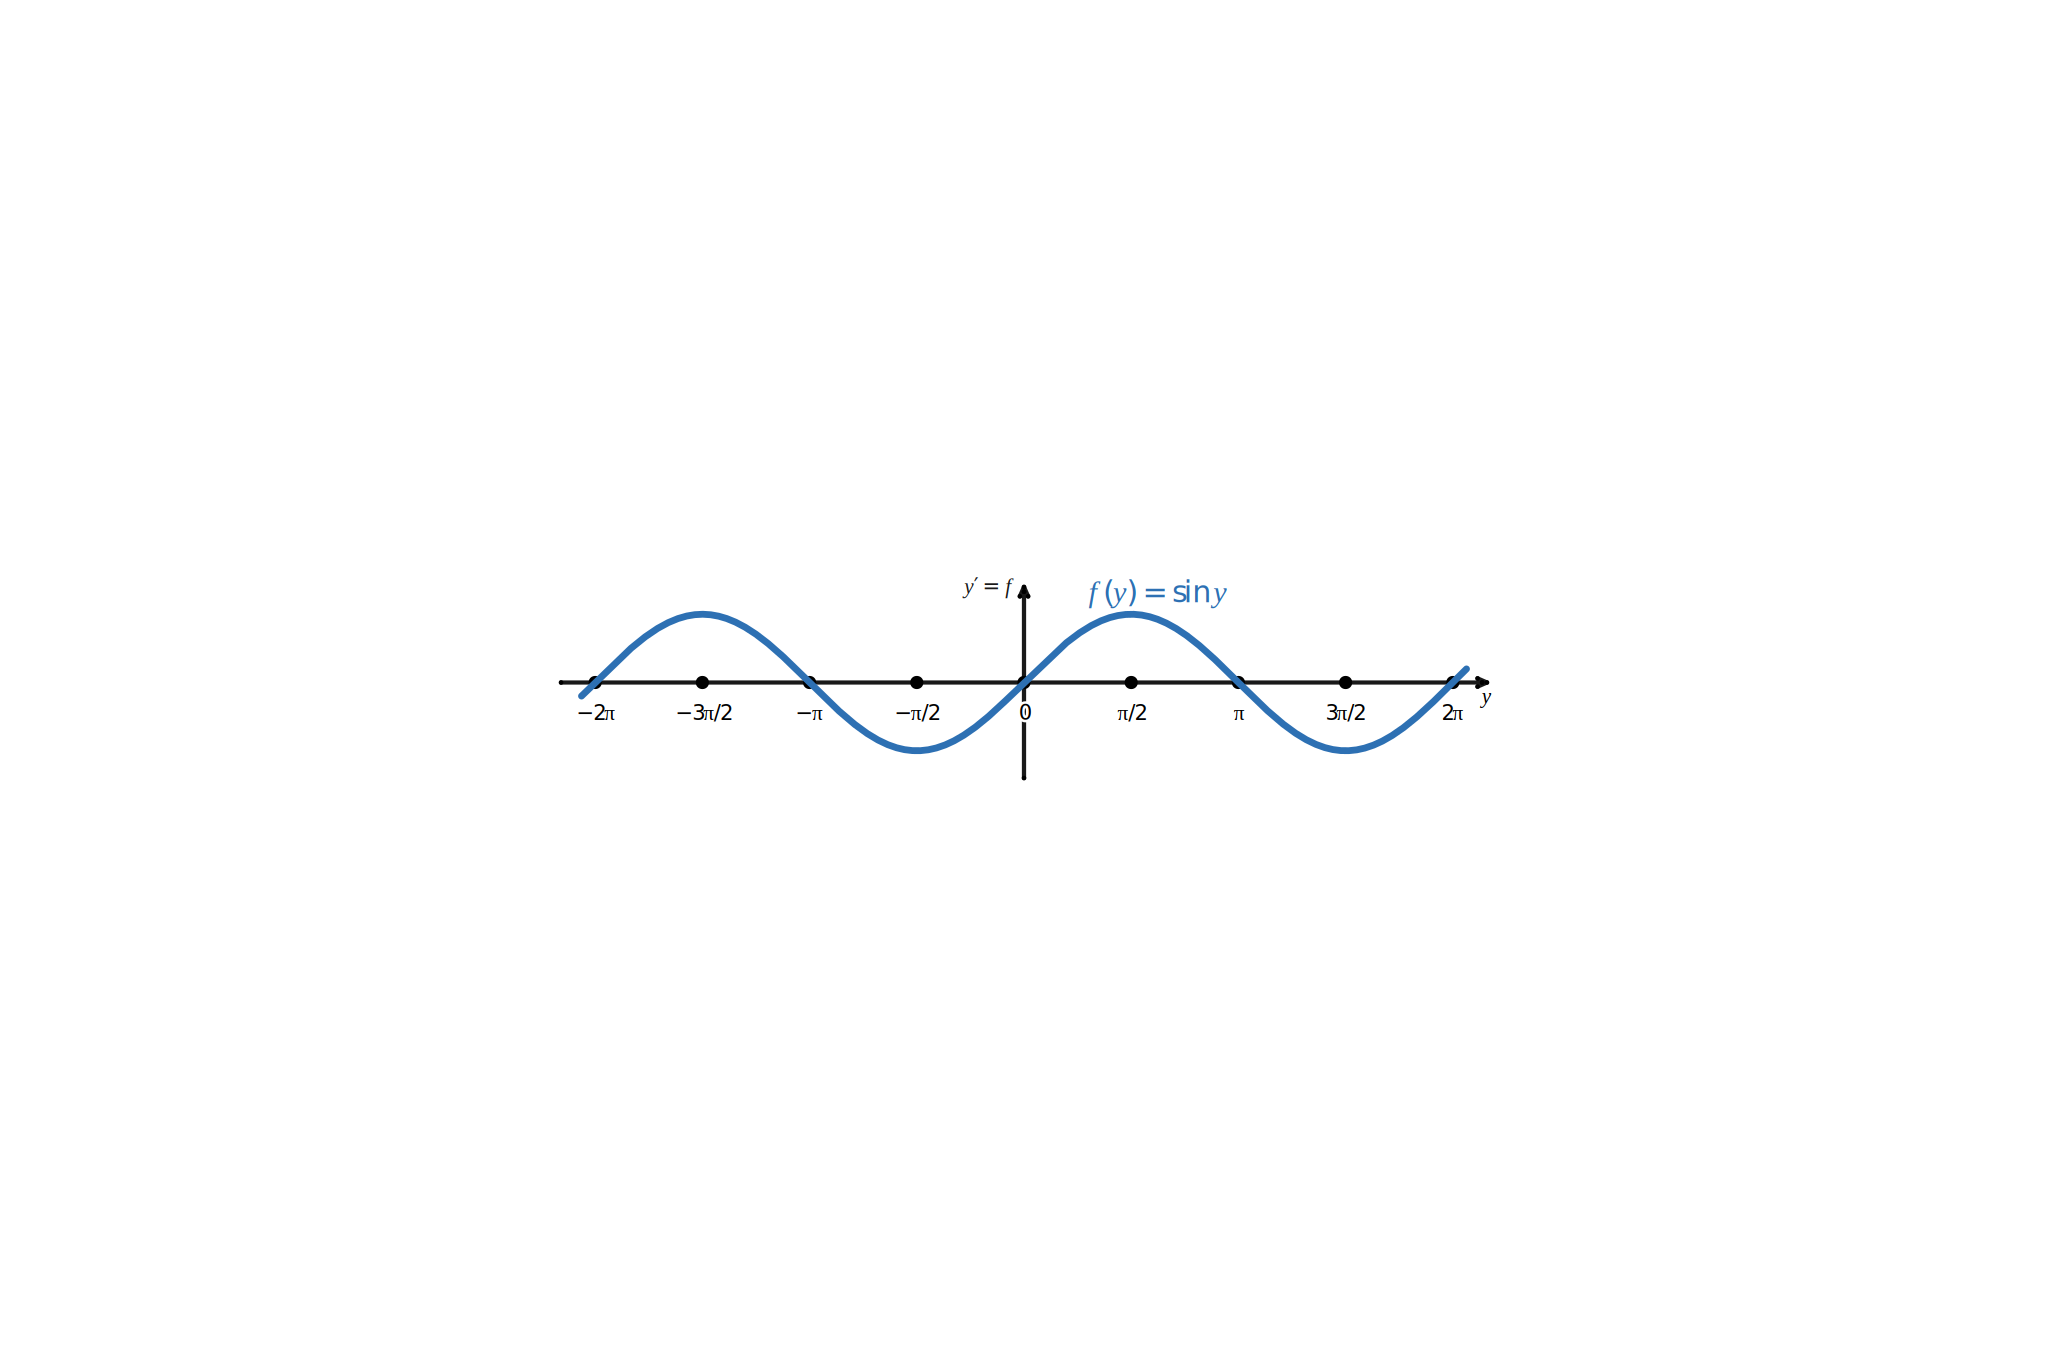
\includegraphics[width=0.9\textwidth]{additional/Stability/func.pdf}
			\caption{График в осях $y'(y)$}
		\end{figure}
		Следующим шагом определим нули производной искомой функции. Для этого необходимо приравнять правую часть $f(y)$ уравнения к нулю:
		\[ \sin{y} = 0 \implies y_n = n\pi, ~ n \in \mathbb{Z}. \]
		Для рассматриваемого случая достаточно условия, что $n = \overline{-2, 2} \subset \mathbb{Z}$. Стоит упомянуть, что для фиксированных значений $n$, $y_n$ является решением следующей задачи:
		\[ y' = \sin{y}, ~ y(0) = y_n. \]
		Такие постоянные $y_n$ называются точками покоя исходного уравнения.

		Теперь у заданной кривой определим участки, где функция $f$ положительна или отрицательна. Эти участки ограничены точками покоя. Решение $y$ уравнения $y' = f(y)$ возрастает, если $f(y) > 0$, и убывает $f(y) < 0$. Эти области пометим соответствующими направляющими стрелками:
		\begin{figure}[H]
			\centering
			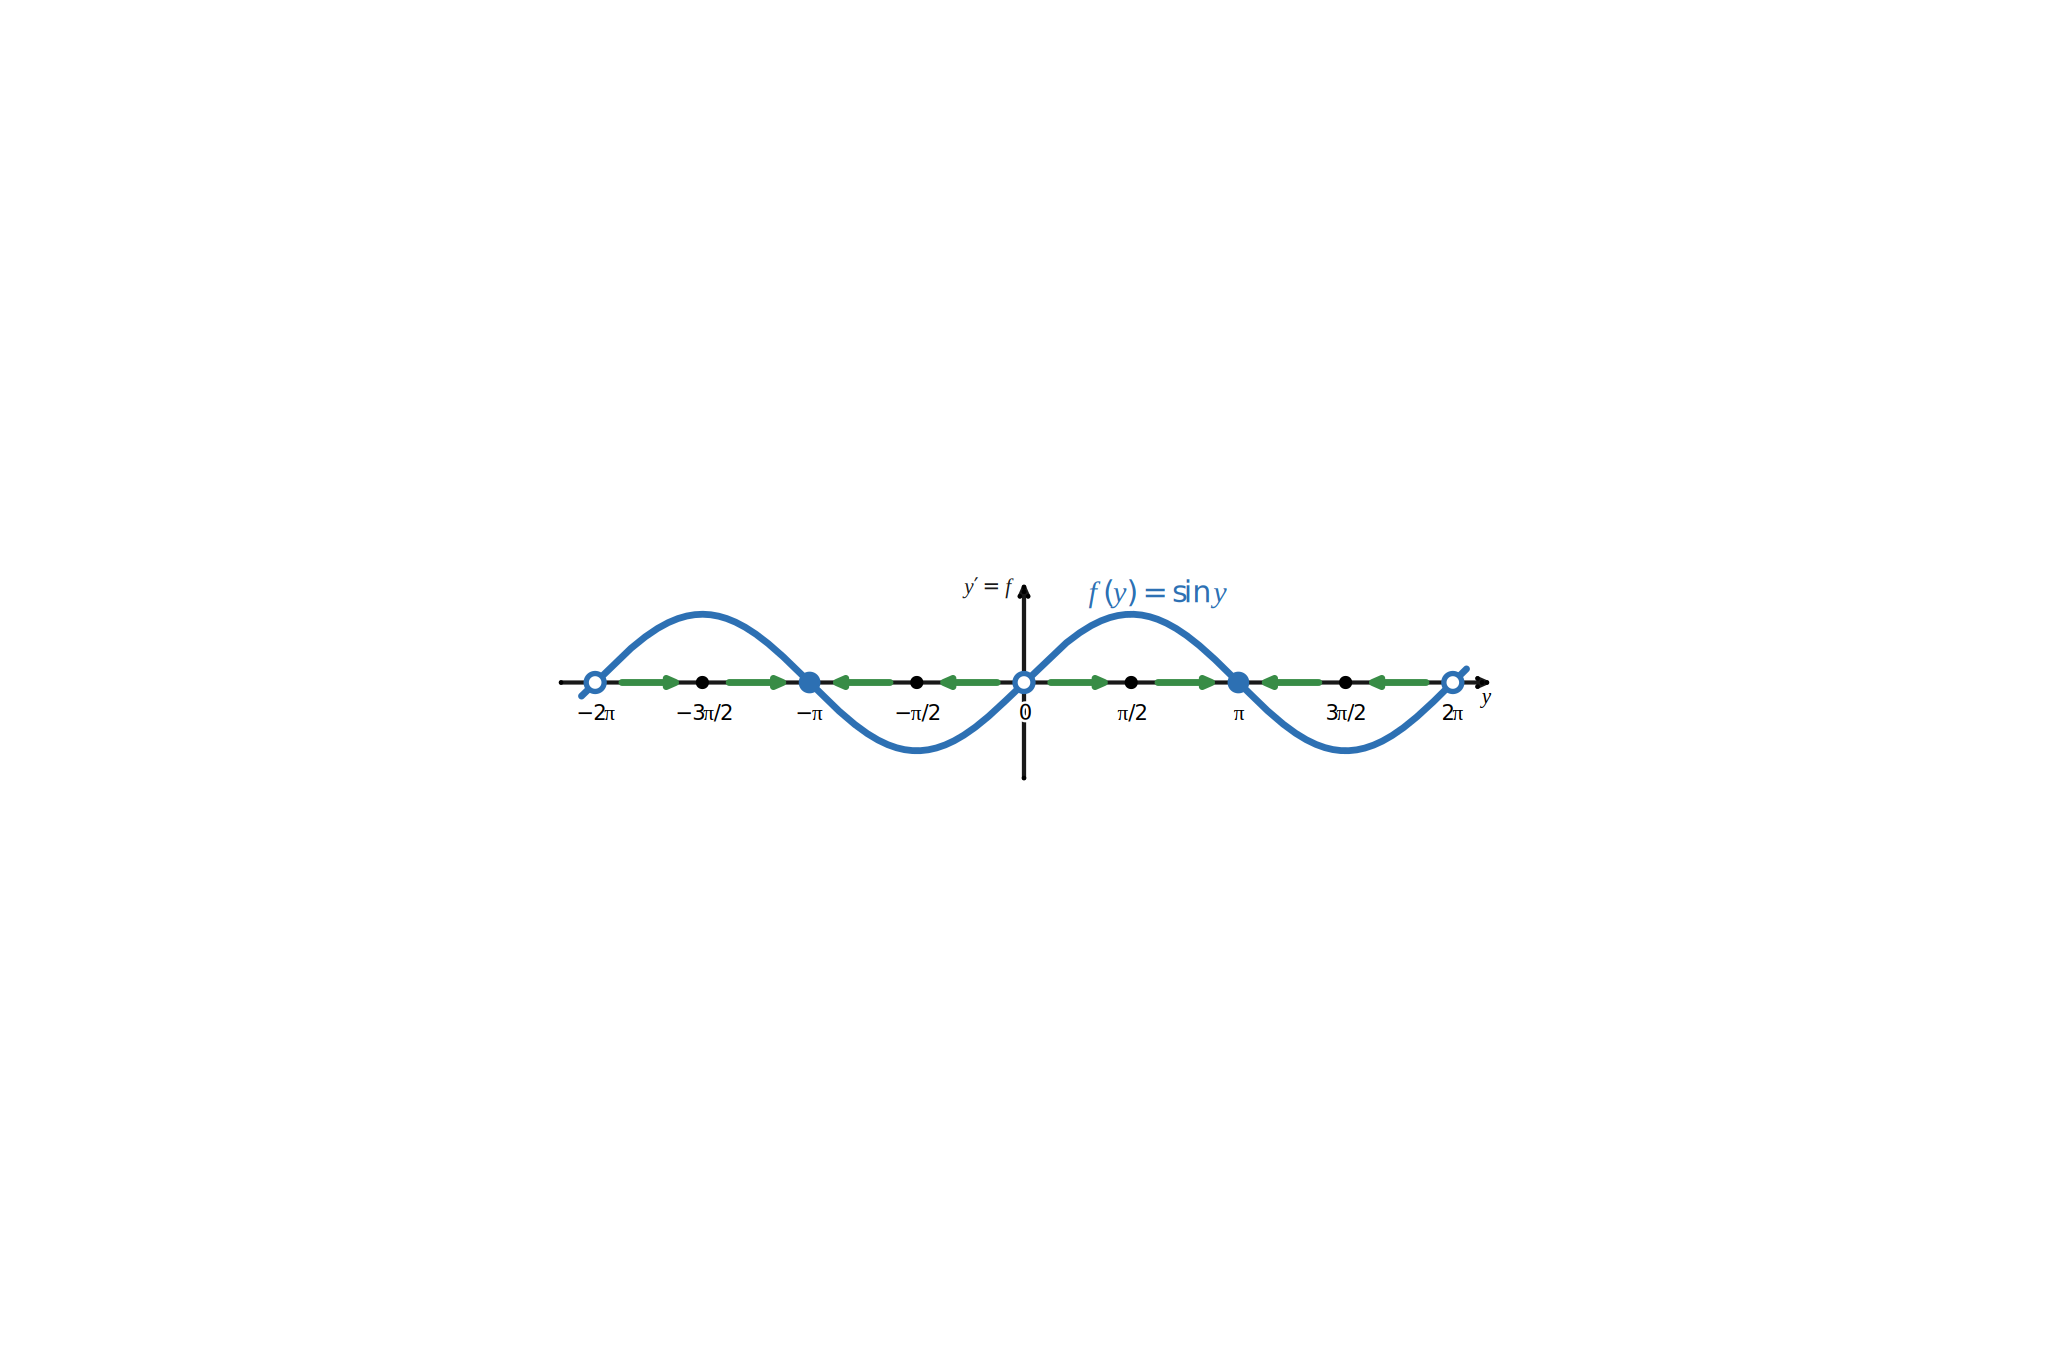
\includegraphics[width=0.9\textwidth]{additional/Stability/func_cv.pdf}
			\caption{График $f(y)$ в осях $y'(y)$ с направлениями в областях возрастания/убывания}
		\end{figure}

		Точки покоя бывают двух типов: устойчивые и неустойчивые соответственно. Согласно направляющим стрелкам, устойчивыми точками будут $y_{-1} = -\pi, ~ y_{1} = \pi$, а неустойчивыми -- $y_{-2} = -2\pi, ~ y_0 = 0, ~ y_{2} = 2\pi$. Теперь построим области перегиба кривых функции. Для этого найдем вторую производную решения:
		\[ y'' = f'(y) \cdot y' = f'(y) \cdot f(y). \]
		Области, где $y'' > 0$ -- вогнуты вверх (выпуклые), и где $y'' < 0$ -- вогнуты вниз (вогнуты).

		\pagebreak
		
		Построим график решения $f'(y)$:
		\begin{figure}[H]
			\centering
			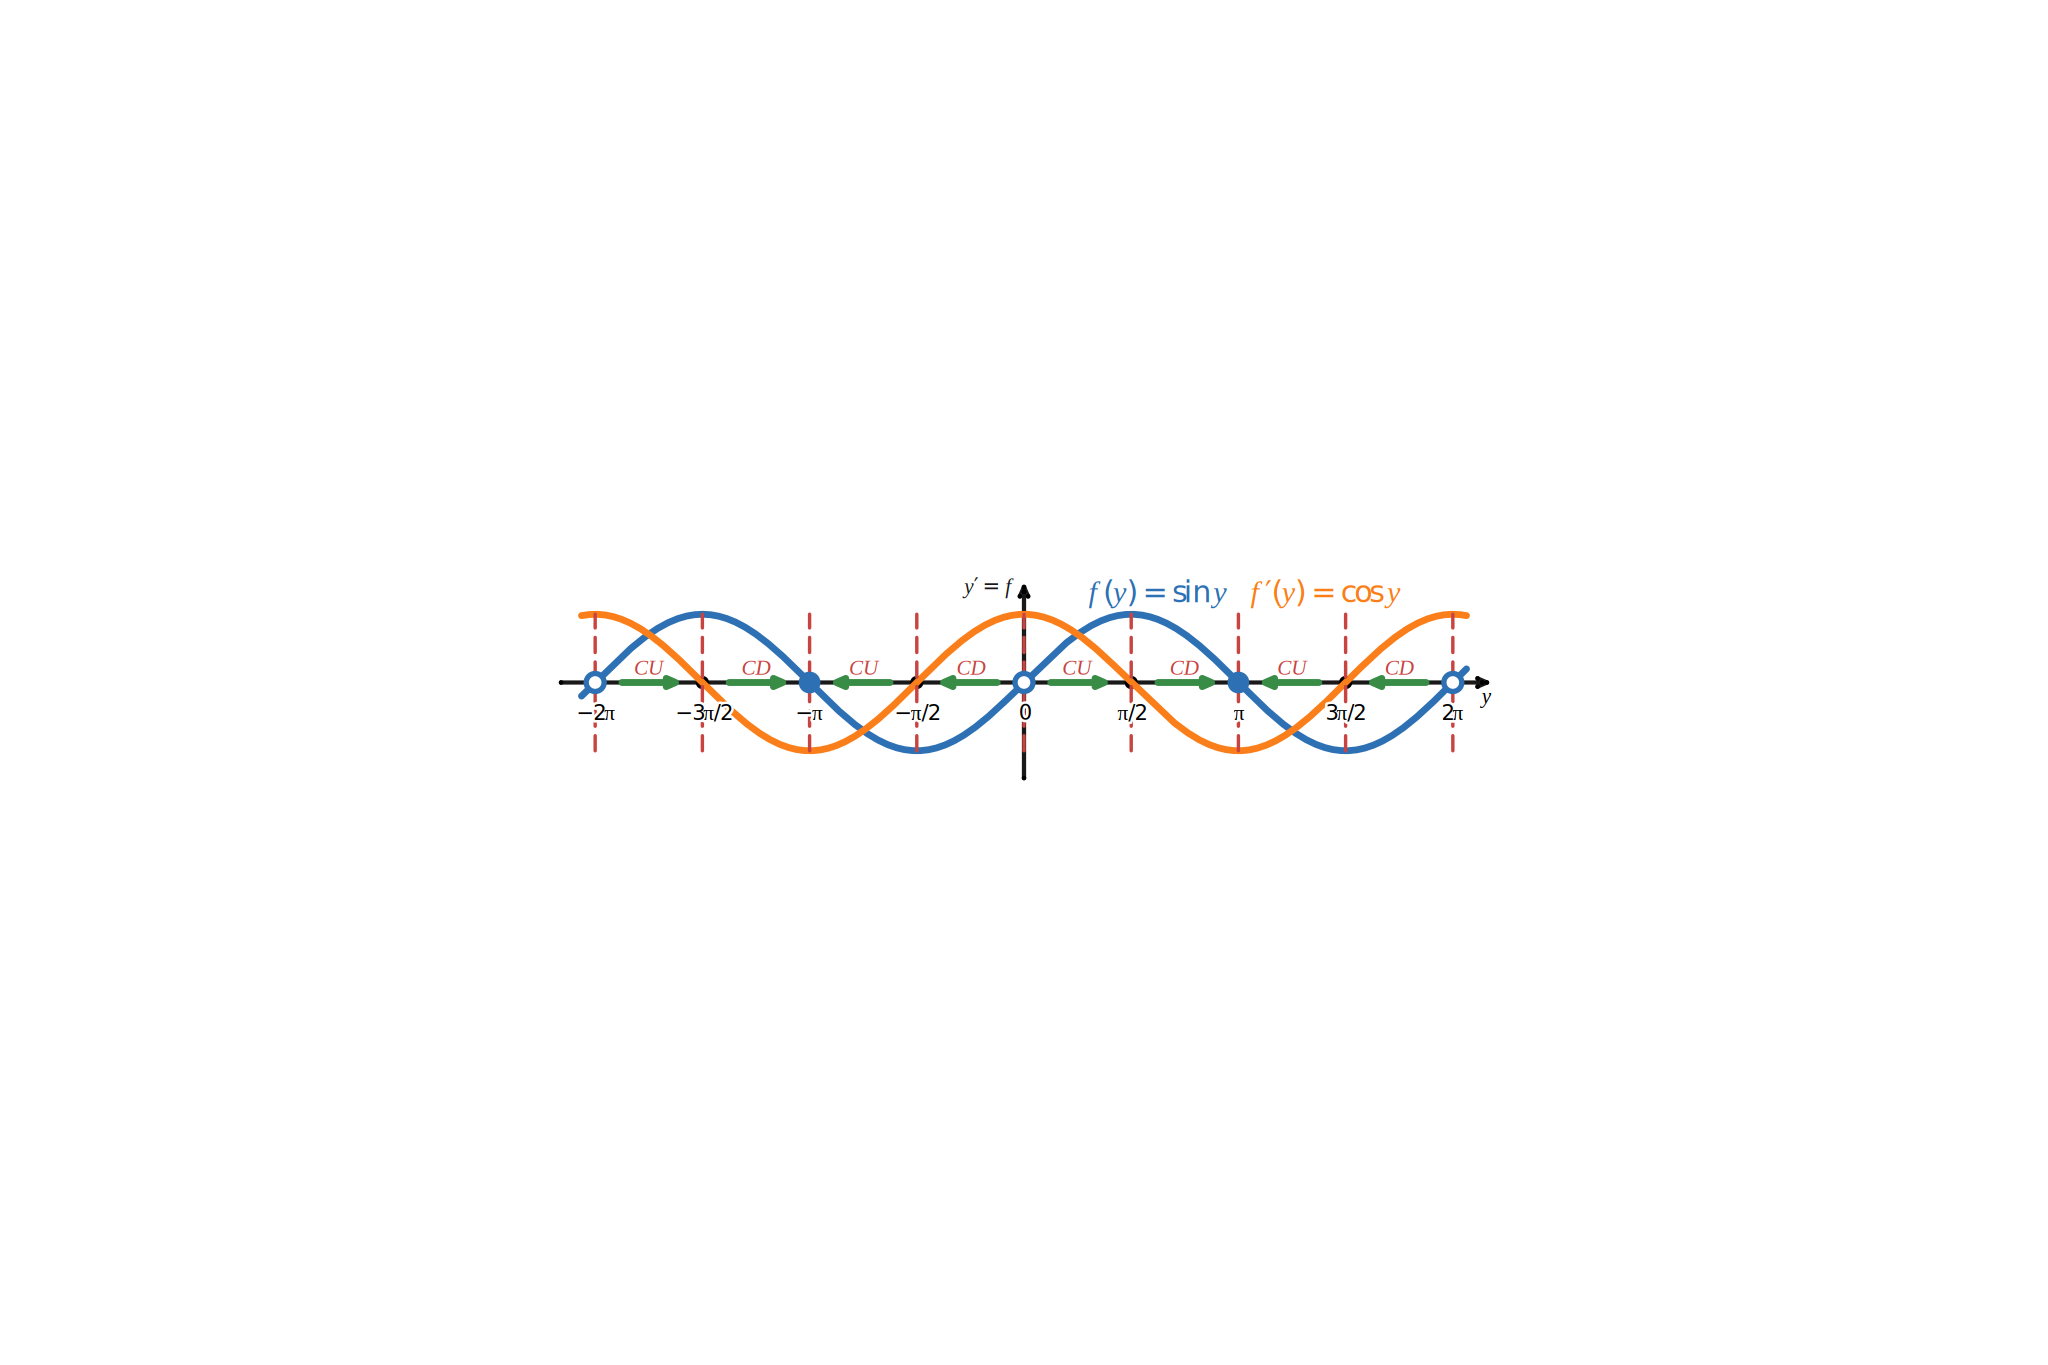
\includegraphics[width=0.9\textwidth]{additional/Stability/func_deriv_cv.pdf}
			\caption{График $f(y)$ и $f'(y)$ в осях $y'(y)$}
		\end{figure}
		На рисунке символами $CU$ и $CD$ помечены участки вогнутости вверх и вниз соответственно. Данной информации достаточно для построения примерного поведения решения исходного уравнения:
		\begin{figure}[H]
			\centering
			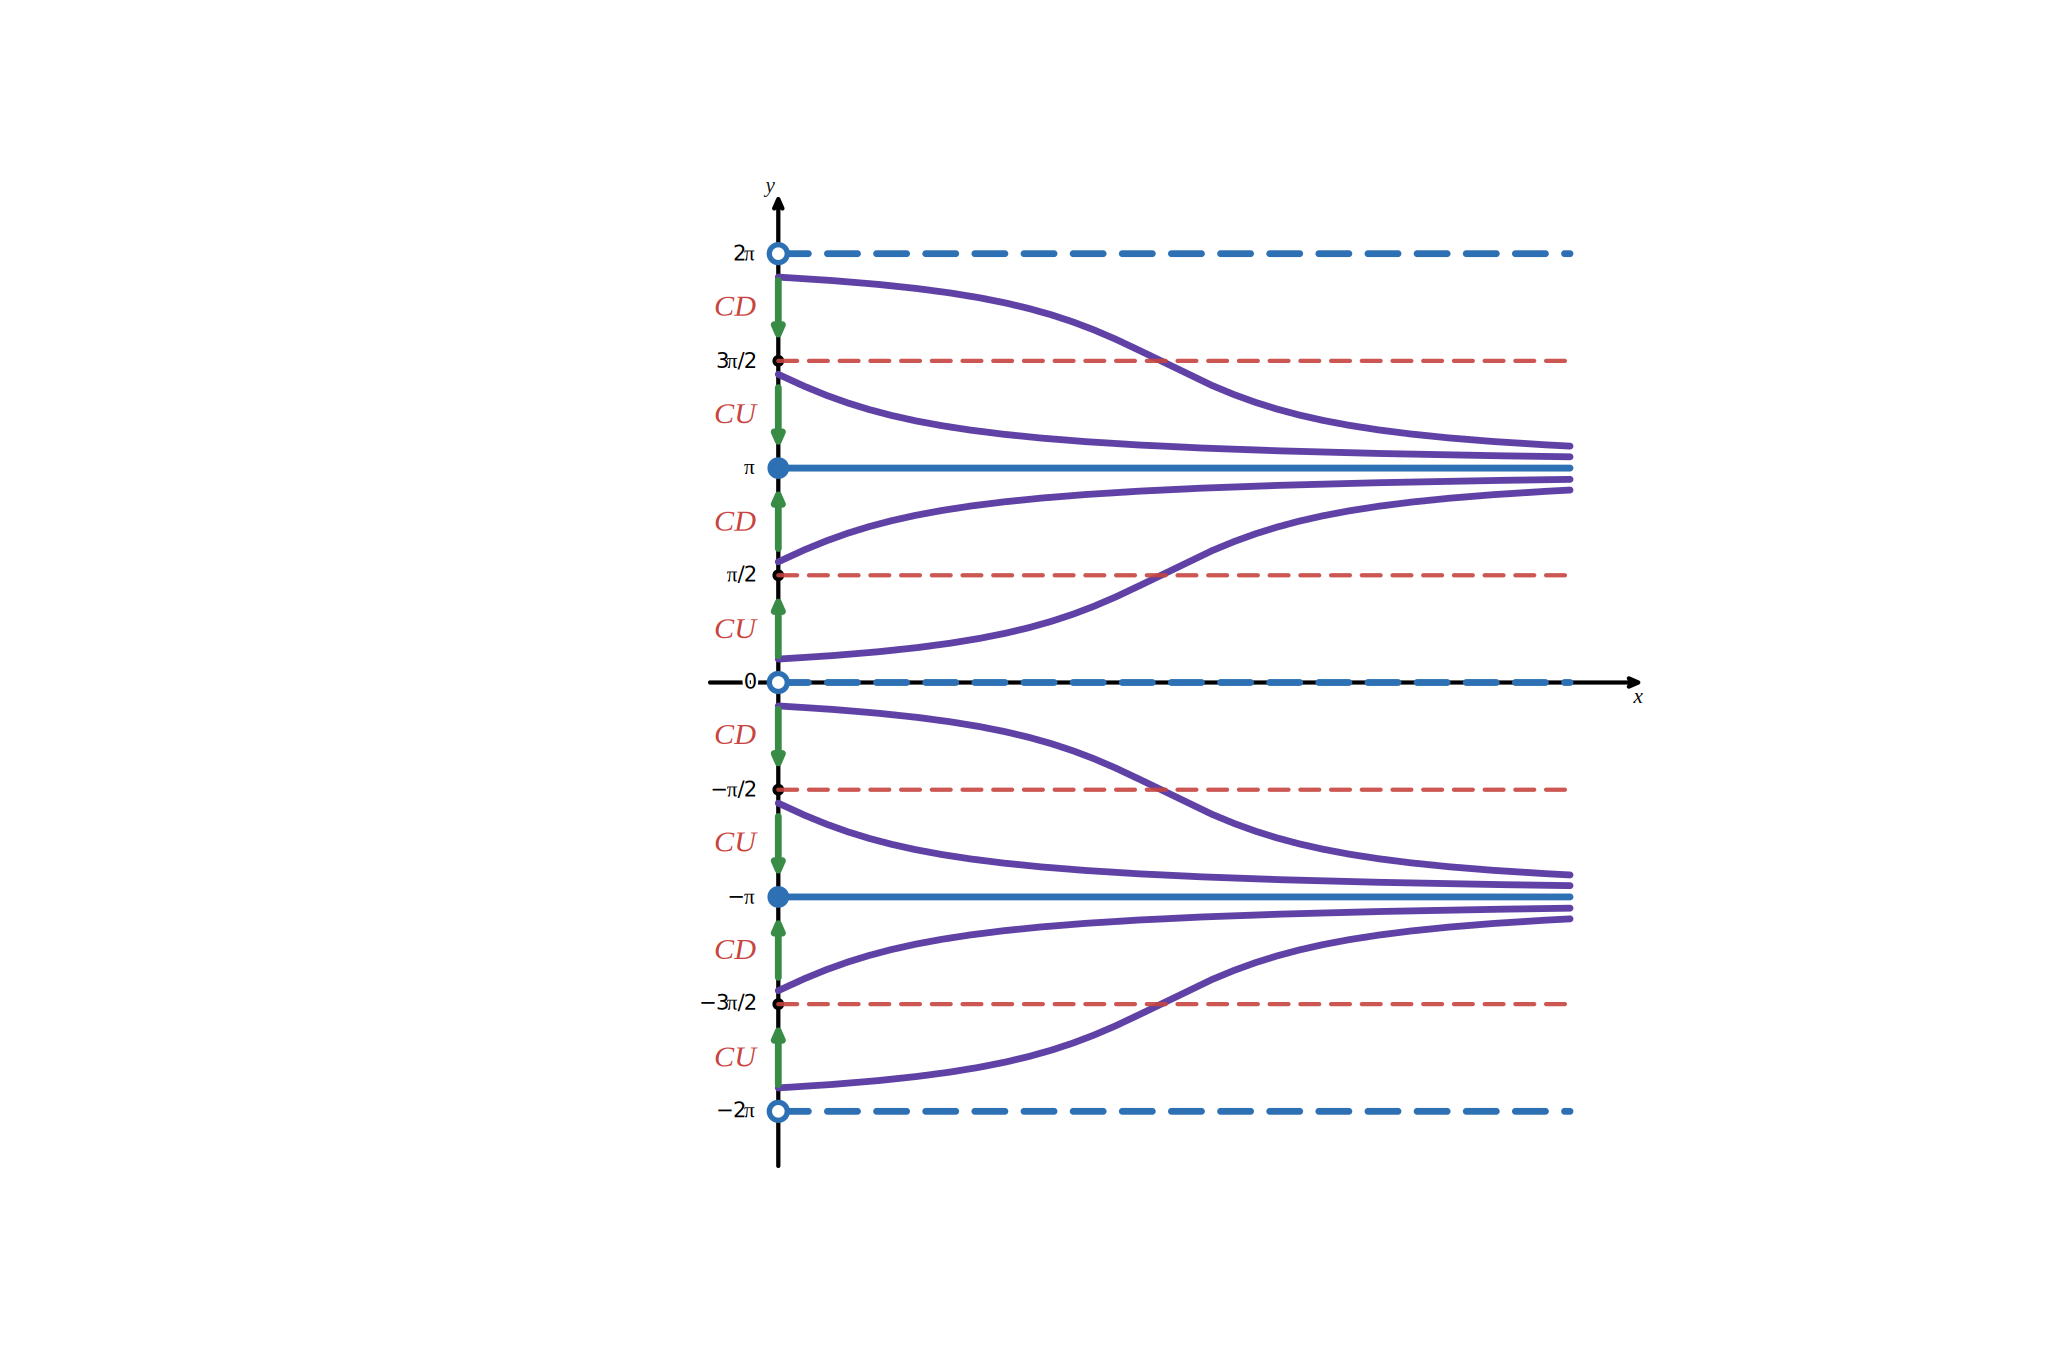
\includegraphics[width=0.8\textwidth]{additional/Stability/sols.pdf}
			\caption{Примерное поведение решения $y(x)$ исходного уравнения}
		\end{figure}

		\pagebreak

		Рассмотрим другой пример. Дана система следующего вида:
		\[ \syst{&\dot{x} = y\sin{x}, \\ &\dot{y} = x\sin{y}}. \]
		Необходимо найти точки покоя, и исследовать их устойчивость. Найдем все возможные точки покоя. Для этого приравняем производные к нулю:
		\[ \syst{&\dot{x} = 0, \\ &\dot{y} = 0.} \implies \syst{&y \sin{x} = 0, \\ &x \sin{y} = 0.} \]
		Из этой системы следует набор таких точек:
		\[ \syst{&x = n\pi, \\ &y = m\pi.}, ~ n, m \in \mathbb{Z} \]
		Построим матрицу Якоби исходной системы в окрестности точки $\pares{n\pi, m\pi}$:
		\[ A = J\pares{x, y} \at_{\pares{n \pi, m \pi}} = \begin{pmatrix} 
			\dpart{}{x}\pares{y \sin{x}} & \dpart{}{y}\pares{y \sin{x}} \\
			\dpart{}{x}\pares{x \sin{y}} & \dpart{}{y}\pares{x \sin{y}}
		\end{pmatrix} \at_{\pares{n \pi, m \pi}} = \begin{pmatrix}
			(-1)^n m \pi & 0 \\
			0 & (-1)^m n \pi
		\end{pmatrix}. \]
		Найдем собственные значения данной матрицы:
		\[ \det{\abs{A - \lambda I}} = 0 \implies \bpares{\lambda - (-1)^n m \pi} \cdot \bpares{\lambda - (-1)^m n \pi} = 0. \]
		Отсюда следует, что $\lambda_1 = (-1)^n m \pi$ и $\lambda_2 = (-1)^m n \pi$. 

		Рассмотрим случаи, когда собственные значения отрицательны одновременно:
		\begin{enumerate}
			\item $n > 0, m > 0$: Если $n$ и $m$ нечетные одновременно;
			\item $n < 0, m < 0$: Если $n$ и $m$ четные одновременно;
			\item $n < 0, m > 0$: Если $n$ -- нечетное, $m$ -- четное;
			\item $n > 0, m < 0$: Если $n$ -- четное, $m$ -- нечетное.
		\end{enumerate}
		Случаи, содержащие $m = 0$, или $n = 0$ не рассматриваем, так как их исследование на устойчивость требует дополнительного анализа. Все остальные случаи сводятся к наличию хотя бы одного положительного собственного значения, что говорит о том, что система не устойчива. В общем случае здесь можно заметить некоторую симметрию относительно $n$ и $m$.

	% \pagebreak
		\subsection{Задачи}

	Найти точки покоя и геометрически исследовать поведение решений:
	\begin{multicols}{2}
		\begin{enumtasks}
			
			\label{stability_zeros:geometrical}
			\item \( y' = y, ~ y \in \pares{-1, 1} \) % \( y = 0 \) -- неуст.;
			\item \( y' = y^2 - 1, ~ y \in \pares{-2, 2} \) % \( y = -1 \) -- уст., \( y = 1 \) -- неуст.;
			\item \( y' = \frac{y}{y + 1}, ~ y \in \pares{-1, 1} \) % \( y = 0 \) -- неуст.;
			\item \( y' = \frac{1 + y}{1 - y}, y \in \pares{-2, 0} \) % \( y = -1 \) -- неуст.;
			\item \( y' = \frac{y^2 - 2y - 3}{y + 3}, ~ y \in \pares{-2, 5} \) % \( y = -1 \) -- неуст., \( y = 3 \) -- уст.;
			\item \( y' = \ln{y}, ~ y \in \pares{0, 2} \) % \( y = 1 \) -- неуст.; 
			\item \( y' = e^y - 1, ~ y \in \pares{-1, 1} \) % \( y = 0 \) -- неуст.;
			\item \( y' = y \ln{y}, ~ y \in (0, 1] \) % \( y = 1 \) -- неуст.;
			\item \( y' = ye^{-y}, ~ y \in \pares{-2, 2} \) % \( y = 0 \) -- неуст.;
			\item \( y' = \sinh{2y}, ~ y \in \pares{-1, 1} \) % \( y = 0 \) -- неуст.;
			
			\label{stability_zeros:geometrical_part2}
			\item \( y' = -e^{-y} \sinh{y}, ~ y \in \pares{-1, 1} \) % \( y = 0 \) -- уст.;
			\item \( y' = \cos{y}, ~ y \in \pares{-2\pi, 2\pi} \) % \( y = -\frac{3\pi}{2}, \frac{\pi}{2} \) -- неуст.; \( y = -\frac{\pi}{2}, \frac{3\pi}{2} \) -- уст.
			\item \( y' = \sin^2{y}, ~ y \in \pares{-2\pi, 2\pi} \) % \( y = -\pi, 0, \pi \) -- стац.;
			\item \( y' = \tan{y}, ~ y \in \pares{-\frac{3\pi}{2}, \frac{3\pi}{2}} \) % \( y = -\pi, 0, \pi \) -- уст.; 
			\item \( y' = 1 - \sec{2y}, ~ y \in \pares{-\frac{3\pi}{2}, \frac{3\pi}{2}} \) % \( y = -\pi, 0, \pi \) -- стац.;
			\item \( y' = \pares{y + 1} \sin{y}, ~ y \in \pares{-\frac{3\pi}{2}, \frac{3\pi}{2}} \) % \( y = -\pi, 0 \) -- уст., \( y = -1, \pi \) -- неуст.;
			\item \( y' = \pares{y - \pi} \cos{y}, ~ y \in \pares{-1, 2\pi} \) % \( y = \pi \) -- уст., \( y = \frac{\pi}{2}, \frac{3\pi}{2} \) -- неуст.;
			\item \( y' = \frac{\cos{y}}{1 - \sin{y}}, ~ y \in \pares{-\pi, 0} \) % \( y = \frac{\pi}{2} \) -- неуст.;
			\item \( y' = \arccot{y} - \frac{\pi}{2}, ~ y \in \pares{-\pi, \pi} \) % \( y = 0 \) -- уст.;
			\item \( y' = y\arctan{\frac{\pi}{y + \pi}}, ~ y \in \pares{-1, 1} \) % \( y = 0 \) -- неуст.;

		\end{enumtasks}
	\end{multicols}

	Найти точки покоя следующих стационарных систем, и исследовать их устойчивость по первому приближению, полагая $x, y \in \mathbb{R}$:
	\begin{multicols}{2}
		\begin{enumtasks}

			\label{stability_zeros:firstapprox2d}
			\item \( \dot{x} = y^2 - x, ~ \dot{y} = x^2 - y \) % \( M_0 \pares{0, 0} \) -- уст., \( M_1 \pares{1, 1} \) -- неуст.;
			\item \( \dot{x} = xy + 1, ~ \dot{y} = x^2 - y^2 \) % \( M_1 \pares{-1, 1} \) -- неуст., \( M_2 \pares{1, -1} \) -- неуст.;
			\item \( \dot{x} = x \pares{y^2 + x}, ~ \dot{y} = y \pares{x^2 - y + 1} \) % \( M_0 \pares{0, 0} \) -- неуст., \( M_1 \pares{0, 1} \) -- неуст.; 
			\item \( \dot{x} = 1 - x^4 - y^2, ~ \dot{y} = x - y - 1 \) % \( M_1 \pares{0, -1} \) -- неуст., \( M_2 \pares{1, 0} \) -- уст.;
			\item \( \dot{x} = \frac{x^2 - 4}{y}, ~ \dot{y} = \frac{y^2 - 1}{x + 1} \) % \( M_1 \pares{-2, -1} \) -- неуст., \( M_2 \pares{-2, 1} \) -- уст., \( M_3 \pares{2, -1} \) -- уст., \( M_4 \pares{2, 1} \) -- неуст.;
			\item \( \dot{x} = y - xe^y, ~ \dot{y} = x^2 - y \) % \( M_0 \pares{0, 0} \) -- уст.;
			\item \( \dot{x} = e^x - e^y, ~ \dot{y} = x^2 + 2y \) % \( M_0 \pares{0, 0} \) -- неуст., \( M_1 \pares{-2, -2} \) -- неуст.;
			\item \( \dot{x} = \sin{y} - x, ~ \dot{y} = - y \cos{x} \) % \( M_0 \pares{0, 0} \) -- уст.;
			\item \( \dot{x} = \frac{\cos{x}}{y^2 - 1}, ~ \dot{y} = xy, ~ x \in \pares{-\pi, \pi} \) % \( M_1 \pares{-\frac{\pi}{2}, 0} \) -- уст., \( M_2 \pares{\frac{\pi}{2}, 0} \) -- неуст.;
			\item \( \dot{x} = \arctan{x} + 2y, ~ \dot{y} = \sinh{x} - \tanh{y} \) % \( M_0 \pares{0, 0} \) -- неуст.;

		\end{enumtasks}
	\end{multicols}

	Найти точки покоя следующих трехмерных стационарных систем, и исследовать их на устойчивость по первому приближению, полагая $x, y, z \in \mathbb{R}$:
	\begin{enumtasks}

		\label{stability_zeros:firstapprox3d}
		\item \( \dot{x} = z - x^2, ~ \dot{y} = y - y^2, ~ \dot{z} = x - z^2 \) % \( M_0 \pares{0, 0, 0} \) -- неуст., \( M_1 \pares{0, 1, 0} \) -- неуст., \( M_2 \pares{1, 0, 1} \) -- неуст., \( M_3 \pares{1, 1, 1} \) -- уст.;
		\item \( \dot{x} = x^2 + y, ~ \dot{y} = z^2 + x^2 y, ~ \dot{z} = 2xz - y^2 \) % \( M_0 \pares{0, 0, 0} \) -- стац., \( M_1 \pares{-2, -4, -4} \) -- уст., \( M_2 \pares{2, -4, 4} \) -- неуст.;
		\item \( \dot{x} = x - y + z - 1, ~ \dot{y} = x^2 + yz, ~ \dot{z} = 1 - z^2 \) % \( M_1 \pares{-1, -1, 1} \) -- неуст., \( M_2 \pares{0, 0, 1} \) -- неуст.;
		\item \( \dot{x} = \sin{x} + \sin{z}, ~ \dot{y} = e^y - e^x, ~ \dot{z} = \cos^2{2z} \) % \( M_1 \pares{-\frac{\pi}{4}, -\frac{\pi}{4}, \frac{\pi}{4}} \) -- неуст., \( M_2 \pares{\frac{\pi}{4}, \frac{\pi}{4}, -\frac{\pi}{4}} \) -- неуст.;

	\end{enumtasks}

	Доказать, что точка $M_0 \pares{0, 0, 0}$ является точкой покоя, и исследовать ее на устойчивость по первому приближению:
	\begin{enumtasks}

		\label{stability_zeros:firstapprox3d_zero}
		\item \( \dot{x} = xy - 2z, ~ \dot{y} = y^2 - x, ~ \dot{z} = y - 2x^2 - 3z \) % \( M_0 \pares{0, 0, 0} \) -- уст.; 
		\item \( \dot{x} = 2 \tan{x} - yz, ~ \dot{y} = 3x^2 - 2y, ~ \dot{z} = \arcsin{z} \) % \( M_0 \pares{0, 0, 0} \) -- неуст.;
		\item \( \dot{x} = x^3 - x, ~ \dot{y} = x - y - 3yz^3, ~ \dot{z} = \sin{x} - 2z \) % \( M_0 \pares{0, 0, 0} \) -- уст.; 
		\item \( \dot{x} = \cos{z} - e^y, ~ \dot{y} = 2\tan{z} + x, ~ \dot{z} = \ln\pares{y+1} - xz \) % \( M_0 \pares{0, 0, 0} \) -- неуст.;
		\item \( \dot{x} = 3z - \arctan{x}, ~ \dot{y} = x^2 - \ln\pares{y+1}, ~ \dot{z} = xy - z \) % \( M_0 \pares{0, 0, 0} \) -- уст.;
		\item \( \dot{x} = \sqrt{xy + 9} - x - 3\cos{z}, ~ \dot{y} = x^2 - \tan\pares{y + z} + z, ~ \dot{z} = \pares{z - 1}^2 + z - e^{-y} \)  % \( M_0 \pares{0, 0, 0} \) -- уст.;

	\end{enumtasks}

		\pagebreak

		%-----------------------------------------------------------------------------------------------------------
		%===========================================================================================================
		%-----------------------------------------------------------------------------------------------------------

		\section{Классификация точек покоя}

	В данном разделе рассмотрим классификацию точек покоя для двумерных вещественных стационарных нелинейных систем обыкновенных дифференциальных уравнений первого порядка:
	\[ \vec{\dot{x}} = \vec{f}\pares{\vec{x}}, ~ \vec{x} = \begin{pmatrix} x_1 \\ x_2 \end{pmatrix} \]

	Для данной системы в окрестности точки покоя $\vec{x} = \vec{x}_0$ будем рассматривать систему первого приближения:
	\[ \vec{\dot{x}} = A \cdot \vec{x}, \]
	где $A = \tilde{J}\pares{\vec{x}} \sat_{\vec{x} = \vec{x}_0}$ -- матрица Якоби в точке покоя, двумерная матрица постоянных коэффициентов. Положим, что матрица $A$ -- разложима с помощью матрицы преобразований $P$, и верхнетреугольной жордановой формы $J$: $A = PJP^{-1}$. Следующая классификация будет рассмотрена для систем вида $\vec{\dot{x}} = J \vec{x}$. Для построения фазового пространства конкретных систем, необходимо построить матрицу преобразований $P$, и по представленным ниже правилам применить матрицу $P$ как матрицу аффинного преобразования системы координат.

	Пусть у матрицы $J$ собственные значения $\lambda_1$ и $\lambda_2$. Собственные вектора $\vec{v}_1, \vec{v}_2$ матрицы $A$ представляют собой соответствующие собственным значениям $\lambda_1, \lambda_2$ столбцы матрицы преобразований $P$. Будем полагать, что собственные вектора рассматриваемой системы равны соответственно $\vec{v}_1 = \begin{pmatrix} 1 \\ 0 \end{pmatrix}$ и $\vec{v}_2 = \begin{pmatrix} 0 \\ 1 \end{pmatrix}$, и соответствующие им прямые на изображениях будут отражены красными линиями. Тогда введем классификацию точек покоя:
	\begin{enumerate}
		\item \textit{Невырожденный узел} -- случай, когда ненулевые вещественные собственные значения $\lambda_{1, 2}$ не равны между собой, и одного знака (положим $\abs{\lambda_1} < \abs{\lambda_2}, ~ \lambda_{1, 2} \in \mathbb{R}, ~ \lambda_{1, 2} \neq 0$). Интегральные кривые на фазовой плоскости сходятся в (в случае отрицательных собственных значений), или исходят из (в случае положительных собственных значений) точки покоя, и изгибаются по направлению прямой, построенной на основе собственного вектора с наименьшим по модулю собственным значением (от прямой с направляющим вектором $\vec{v}_2$ к прямой с направляющим вектором $\vec{v}_1$). На изображениях ниже рассмотрены случаи $J = \begin{pmatrix} -1 & 0 \\ 0 & -2 \end{pmatrix}$ (устойчивый невырожденный узел, рис. \ref{Stability:StableKnot}) и $J = \begin{pmatrix} 2 & 0 \\ 0 & 3 \end{pmatrix}$ (неустойчивый невырожденный узел, рис. \ref{Stability:UnstableKnot}).

			\begin{multicols}{2}

				\begin{figure}[H]
					\centering
					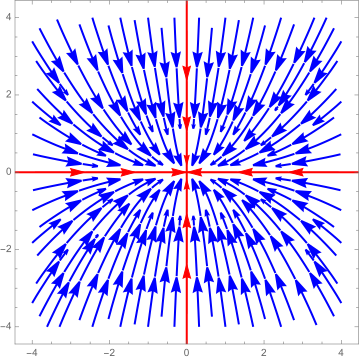
\includegraphics[width=0.4\textwidth]{additional/Stability/Points/StableKnot.pdf}
					\caption{Устойчивый невырожденный узел}
					\label{Stability:StableKnot}
				\end{figure}

			\columnbreak

				\begin{figure}[H]
					\centering
					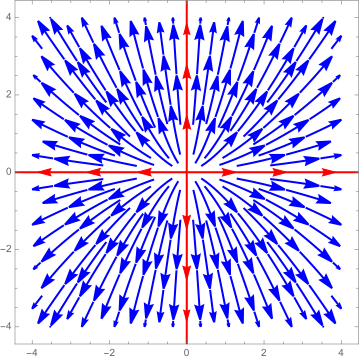
\includegraphics[width=0.4\textwidth]{additional/Stability/Points/UnstableKnot.pdf}
					\caption{Неустойчивый невырожденный узел}
					\label{Stability:UnstableKnot}
				\end{figure}

			\end{multicols}

		\item \textit{Вырожденный узел} -- случай, когда ненулевые вещественные собственные значения $\lambda_{1, 2}$ равны между собой, при этом линейно-зависимы (положим $\lambda_1 = \lambda_2 = \lambda \neq 0, ~ \lambda \in \mathbb{R}$). Интегральные кривые на фазовой плоскости сходятся в (в случае отрицательных собственных значений), или исходят из (в случае положительных собственных значений) точки покоя, и вращаются в направлении, обратном положительному направлению вращения системы координат (против часовой стрелки). На изображениях ниже рассмотрены случаи $J = \begin{pmatrix} -2 & 1 \\ 0 & -2 \end{pmatrix}$ (устойчивый вырожденный узел, рис. \ref{Stability:StableDegKnot}) и $J = \begin{pmatrix} 3 & 1 \\ 0 & 3 \end{pmatrix}$ (неустойчивый вырожденный узел, рис. \ref{Stability:UnstableDegKnot}).

			\begin{multicols}{2}

				\begin{figure}[H]
					\centering
					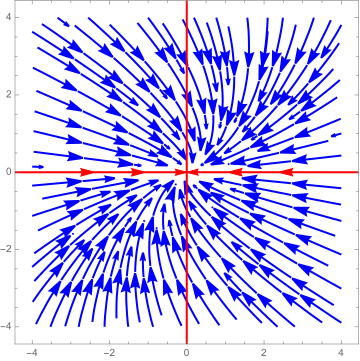
\includegraphics[width=0.4\textwidth]{additional/Stability/Points/StableDegKnot.pdf}
					\caption{Устойчивый вырожденный узел}
					\label{Stability:StableDegKnot}
				\end{figure}

			\columnbreak

				\begin{figure}[H]
					\centering
					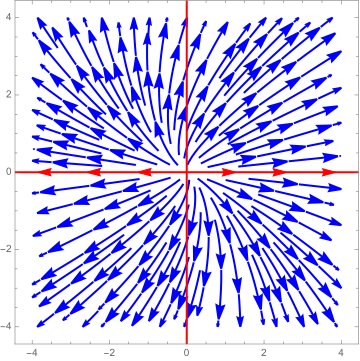
\includegraphics[width=0.4\textwidth]{additional/Stability/Points/UnstableDegKnot.pdf}
					\caption{Неустойчивый вырожденный узел}
					\label{Stability:UnstableDegKnot}
				\end{figure}

			\end{multicols}

		\item \textit{Дикритический узел} -- случай, когда ненулевые вещественные собственные значения $\lambda_{1, 2}$ равны между собой, при этом линейно-независимы (положим $\lambda_1 = \lambda_2 = \lambda \neq 0, ~ \lambda \in \mathbb{R}$). Интегральные кривые на фазовой плоскости сходятся в (в случае отрицательных собственных значений), или исходят из (в случае положительных собственных значений) точки покоя, и представляют собой прямые линии. На изображениях ниже рассмотрены случаи $J = \begin{pmatrix} -1 & 0 \\ 0 & -1 \end{pmatrix}$ (устойчивый дикритический узел, рис. \ref{Stability:StableDicritKnot}) и $J = \begin{pmatrix} 2 & 0 \\ 0 & 2 \end{pmatrix}$ (неустойчивый дикритический узел, рис. \ref{Stability:UnstableDicritKnot}).

			\begin{multicols}{2}

				\begin{figure}[H]
					\centering
					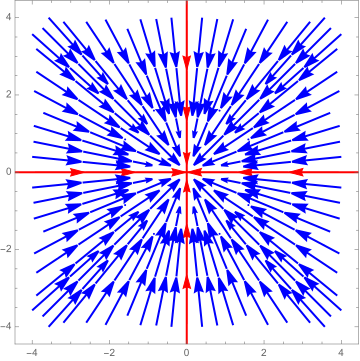
\includegraphics[width=0.4\textwidth]{additional/Stability/Points/StableDicritKnot.pdf}
					\caption{Устойчивый дикритический узел}
					\label{Stability:StableDicritKnot}
				\end{figure}

			\columnbreak

				\begin{figure}[H]
					\centering
					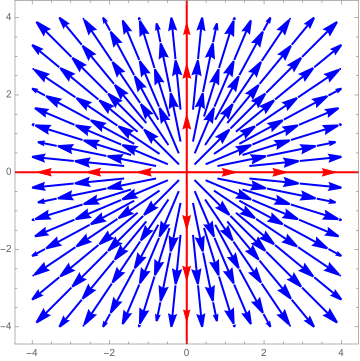
\includegraphics[width=0.4\textwidth]{additional/Stability/Points/UnstableDicritKnot.pdf}
					\caption{Неустойчивый дикритический узел}
					\label{Stability:UnstableDicritKnot}
				\end{figure}

			\end{multicols}

		\item \textit{Седло} -- случай, когда ненулевые вещественные собственные значения $\lambda_{1, 2}$ имеют противоположные знаки (положим $\lambda_1 < 0 < \lambda_2, ~ \lambda_{1, 2} \in \mathbb{R}$). Интегральные кривые на фазовой плоскости представляют собой семейство гипербол в окрестности точки покоя. Направление задается от прямой, построенной на основе собственного вектора с положительным собственным значением в сторону прямой, построенной на основе собственного вектора с отрицательным собственным значением. Седловая точка является неустойчивой. На изображении ниже рассмотрен случай $J = \begin{pmatrix} -1 & 0 \\ 0 & 2 \end{pmatrix}$ (седловая точка, рис. \ref{Stability:Saddle}).

			\begin{figure}[H]
				\centering
				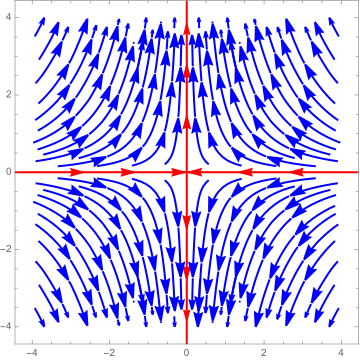
\includegraphics[width=0.4\textwidth]{additional/Stability/Points/Saddle.pdf}
				\caption{Неустойчивая седловая точка}
				\label{Stability:Saddle}
			\end{figure}

		\item \textit{Фокус} -- случай, когда комплексно-сопряженные собственные значения $\lambda_{1, 2}$ имеют ненулевую вещественную часть (положим $\lambda_{1, 2} = \alpha \pm i \beta, ~ \alpha, \beta \in \mathbb{R}, ~ \lambda_{1, 2} \in \mathbb{C}$). Интегральные кривые представляют собой вращающийся поток, сходящийся к (в случае отрицательной вещественной части собственных значений), или исходящихся от (в случае положительной вещественной части собственных значений) точки покоя (при этом ее не касается). Вращение производится в положительном направлении вращения системы координат (по часовой стрелке) в случае, если вещественная жорданова форма является обобщением комплексного числа. На изображениях ниже рассмотрены случаи $J = \begin{pmatrix} -1 & -2 \\ 2 & -1 \end{pmatrix}$ (устойчивый фокус, рис. \ref{Stability:StableFocal}) и $J = \begin{pmatrix} 2 & -1 \\ 1 & 2 \end{pmatrix}$ (неустойчивый фокус, рис. \ref{Stability:UnstableFocal}).

			\begin{multicols}{2}

				\begin{figure}[H]
					\centering
					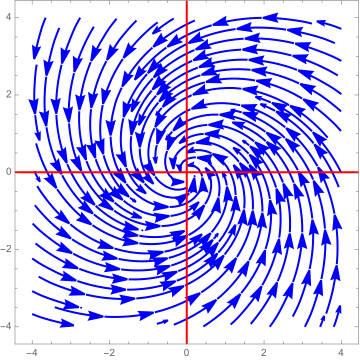
\includegraphics[width=0.4\textwidth]{additional/Stability/Points/StableFocal.pdf}
					\caption{Устойчивый фокус}
					\label{Stability:StableFocal}
				\end{figure}

			\columnbreak

				\begin{figure}[H]
					\centering
					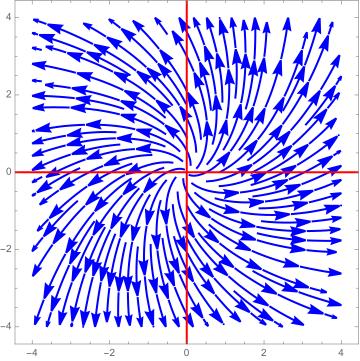
\includegraphics[width=0.4\textwidth]{additional/Stability/Points/UnstableFocal.pdf}
					\caption{Неустойчивый фокус}
					\label{Stability:UnstableFocal}
				\end{figure}

			\end{multicols}

		\item \textit{Центр} -- случай, когда комплексно-сопряженные собственные значения $\lambda_{1, 2}$ имеют нулевую вещественную часть (положим $\lambda_{1, 2} = \pm i \beta, ~ \beta \in \mathbb{R}, ~ \lambda_{1, 2} \in \mathbb{C}$). Интегральные кривые представляют собой семейство эллипсов, окружающих точку покоя. Вращение производится в положительном направлении вращения системы координат (по часовой стрелке) в случае, если вещественная жорданова форма является обобщением комплексного числа. На изображении ниже рассмотрен случай $J = \begin{pmatrix} 0 & -1 \\ 1 & 0 \end{pmatrix}$ (устойчивый фокус, рис. \ref{Stability:Circular}). 

			\begin{figure}[H]
				\centering
				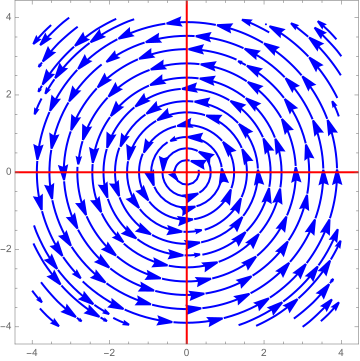
\includegraphics[width=0.4\textwidth]{additional/Stability/Points/Circular.pdf}
				\caption{Центр}
				\label{Stability:Circular}
			\end{figure}

		\item \textit{Семейство параллельных прямых} -- случай, когда среди вещественных собственных значений $\lambda_{1, 2}$ имеется хотя-бы одно отрицательное собственное значение (положим $\lambda_1 = 0, \lambda_2 \neq 0, ~ \lambda_{1, 2} \in \mathbb{R}$). В случае, если хотя бы одно из собственных значений не нулевое, интегральные кривые представляют собой параллельные прямые, параллельные прямой, образованной собственным вектором, отвечающим ненулевому собственному значению, и сходящиеся к (в случае одного отрицательного собственного значения), или исходящие из (в случае одного положительного собственного значения) прямой, образованной собственным вектором, отвечающим за нулевое собственное значение. На изображениях ниже рассмотрены случаи $J = \begin{pmatrix} -2 & 0 \\ 0 & 0 \end{pmatrix}$ (устойчивое семейство параллельных прямых, рис. \ref{Stability:StableParallel}) и $J = \begin{pmatrix} 1 & 0 \\ 0 & 0 \end{pmatrix}$ (неустойчивое семейство параллельных прямых, рис. \ref{Stability:UnstableParallel}).

			\begin{multicols}{2}

				\begin{figure}[H]
					\centering
					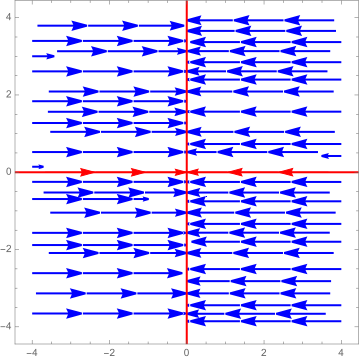
\includegraphics[width=0.35\textwidth]{additional/Stability/Points/StableParallel.pdf}
					\caption{Сходящееся семейство параллельных прямых}
					\label{Stability:StableParallel}
				\end{figure}

			\columnbreak

				\begin{figure}[H]
					\centering
					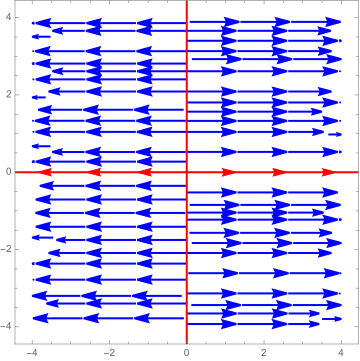
\includegraphics[width=0.35\textwidth]{additional/Stability/Points/UnstableParallel.pdf}
					\caption{Расходящееся семейство параллельных прямых}
					\label{Stability:UnstableParallel}
				\end{figure}

			\end{multicols}

			В случае, если оба собственных значения нулевые, и линейно-зависимы (положим $\lambda_1 = \lambda_2 = 0$), то параллельные прямые разнонаправлены. Выше прямой, образованной первым направляющим вектором параллельные прямые направлены в сторону его положительного направления, ниже -- отрицательного. В случае, когда нулевые значения линейно-независимы, фазовое пространство находится в покое. На изображении ниже рассмотрен случай $J = \begin{pmatrix} 0 & 1 \\ 0 & 0 \end{pmatrix}$ (неустойчивое семейство параллельных разнонаправленных прямых, рис. \ref{Stability:UnstableLinearFlow})
			
			\begin{figure}[H]
				\centering
				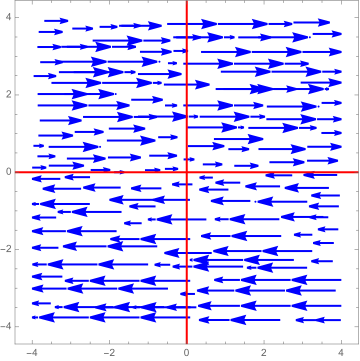
\includegraphics[width=0.5\textwidth]{additional/Stability/Points/UnstableLinearFlow.pdf}
				\caption{Неустойчивое семейство параллельных разнонаправленных прямых}
				\label{Stability:UnstableLinearFlow}
			\end{figure}

	\end{enumerate}


	\subsection{Примеры}

		В качестве примера рассмотрим следующую систему нелинейных дифференциальных уравнений:
		\[ \syst{\dot{x} &= y \cos{x}, \\ \dot{y} &= \sin{x}.} \]
		Найдем ее стационарные точки. Для это построим решение следующей системы:
		\[ \syst{&y \cos{x} = 0 \\ &\sin{x} = 0} \implies \syst{x &= \pi k, ~ k \in \mathbb{Z}, \\ y &= 0.} \]
		Построим соответствующую линеаризованную систему в окрестности точек $M_k = \pares{\pi k, 0}$:
		\[ 
			\tilde{J} \pares{x, y} \sat_{x = \pi k, ~ y = 0} = 
			\begin{pmatrix}
				-y \sin{x} & \cos{x} \\ \cos{x} & 0
			\end{pmatrix} \sat_{x = \pi k, ~ y = 0} = 
			\begin{pmatrix}
				0 & (-1)^k \\ (-1)^k & 0
			\end{pmatrix}
		\]
		Собственные значения матрицы: $\lambda_{1, 2} = \pm 1$ -- вещественные, разных знаков, соответственно точки $M_k = \pares{\pi k, 0}$ являются седловыми. Собственные вектора матрицы:
		\[ \lambda_1 = -1: \vec{v}_1 = \begin{pmatrix} (-1)^k \\ -1 \end{pmatrix}, ~ \lambda_2 = 1: \vec{v}_2 = \begin{pmatrix} (-1)^k \\ 1 \end{pmatrix}. \]
		Матрица преобразования, и жорданова форма имеют следующий вид:
		\[ P = \begin{pmatrix} (-1)^k & (-1)^k \\ -1 & 1 \end{pmatrix}, ~ J = \begin{pmatrix} -1 & 0 \\ 0 & 1 \end{pmatrix}. \]
		Применим преобразование $P$ для фазового пространства, описанного на рис. (\ref{Stability:Saddle}):
		\begin{multicols}{2}

			\begin{figure}[H]
				\centering
				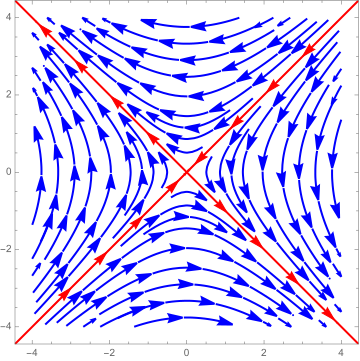
\includegraphics[width=0.35\textwidth]{additional/Stability/Points/Example1Odd.pdf}
				\caption{Седловая точка в случае $k$ -- нечетных}
				\label{Stability:Example1Odd}
			\end{figure}

		\columnbreak

			\begin{figure}[H]
				\centering
				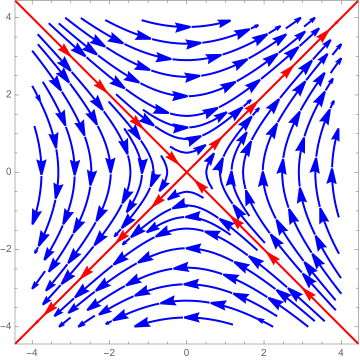
\includegraphics[width=0.35\textwidth]{additional/Stability/Points/Example1Even.pdf}
				\caption{Седловая точка в случае $k$ -- четных}
				\label{Stability:Example1Even}
			\end{figure}

		\end{multicols}
		Объединим данные траектории на общем изображении:
		\begin{figure}[H]
			\centering
			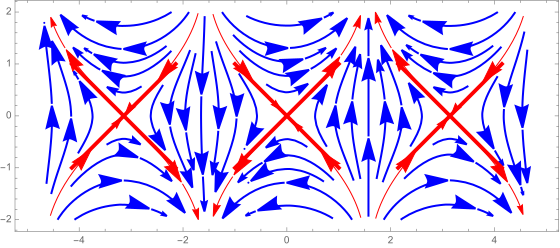
\includegraphics[width=0.7\textwidth]{additional/Stability/Points/Example1Sol.pdf}
			\caption{Фазовое пространство решения}
			\label{Stability:Example1Sol}
		\end{figure}

		Рассмотрим следующий пример:
		\[ \left\lbrace \begin{split}
			\dot{x} &= - 2 x^2 y - 2 x y^2 - 2 y^2 + 22 y \\
			\dot{y} &= 2 x^2 y - 2 x y + 2 y^2 - 22 y
		\end{split} \right. \]
		Найдем нули системы:
		\[ 
			\syst{
				&y \pares{x^2 + xy + y - 11} = 0 \\ &y \pares{x^2 - x + y - 11} = 0 
			} \implies \begin{split} 
				&M_0 = \pares{C, 0}, ~ M_1 = \pares{0, 11}, \\ 
				&M_2 = \pares{-3, -1}, ~ M_3 = \pares{4, -1}. 
			\end{split} 
		\]
		Матрица Якоби исходной системы имеет следующий вид: 
		\[
			\tilde{J} = \begin{pmatrix}
				- 4xy - 2y^2 & - 2 x^2 - 4xy - 4y + 22 \\ 
				4xy - 2y & 2 x^2 - 2x + 4y - 22
			\end{pmatrix}
		\]

		Рассмотрим точку $M_0$. Матрица Якоби в окрестности точки $M_0$ принимает вид:
		\[
			\tilde{J} = \begin{pmatrix}
				0 & 22 - 2C^2 \\
				0 & -22 + 2C^2
			\end{pmatrix}
		\]
		Собственные значения и соответствующие им собственные вектора следующие:
		\[ \lambda_1 = 0: \vec{v}_1 = \begin{pmatrix} 1 \\ 0 \end{pmatrix}, ~ \lambda_2 = -22 + 2C^2: \vec{v}_2 = \begin{pmatrix} 1 \\ -1 \end{pmatrix}. \]
		Так как среди собственных значений присутствует хотя-бы один ноль, то точка $M_0 \forall C$ является семейством параллельных прямых. В случае, если $C^2 < 11$ -- интегральные прямые сходятся к прямой, образованной вектором $\vec{v}_1$ перпендикулярно вектору $\vec{v}_2$; если $C^2 > 11$ -- интегральные прямые исходят из прямой, образованной вектором $\vec{v}_1$ перпендикулярно вектору $\vec{v}_2$; если $C^2 = 11$, то окрестность находится в состоянии покоя.

		Рассмотрим точку $M_1$. Матрица Якоби в окрестности точки $M_1$ принимает вид:
		\[
			\tilde{J} = \begin{pmatrix}
				-242 & -22 \\
				-22 & 22
			\end{pmatrix}
		\]
		Собственные значения и соответствующие им собственные вектора следующие:
		\[ \lambda_{1, 2} = 22 \pares{-5 \pm \sqrt{37}}: \vec{v}_{1, 2} = \begin{pmatrix} 6 \pm \sqrt{37} \\ 1 \end{pmatrix}. \]
		Собственные значения разных знаков, тогда точка $M_1$ -- неустойчивая седловая точка. Интегральные кривые сходятся вдоль прямой, образованной вектором $\vec{v}_2$, и расходятся вдоль прямой, образованной вектором $\vec{v}_1$.

		Рассмотрим точку $M_2$. Матрица Якоби в окрестности точки $M_2$ принимает вид:
		\[
			\tilde{J} = \begin{pmatrix}
				-14 & -4 \\
				14 & -2
			\end{pmatrix}
		\]
		Собственные значения и соответствующие им собственные вектора следующие:
		\[ \lambda_{1, 2} = -8 \pm i \cdot 2\sqrt{5}: \vec{v}_{1, 2} = \begin{pmatrix} -3 \pm i \sqrt{5} \\ 7 \end{pmatrix}. \]
		Оба собственных значения комплексные, с отрицательной вещественной частью, тогда точка $M_2$ -- устойчивый фокус. Вещественная матрица преобразования и матрица комплексного числа примут следующий вид:
		\[ P = \begin{pmatrix} 2 & -2 \\ \sqrt{5} - 3 & \sqrt{5} + 3 \end{pmatrix}, ~ J = \begin{pmatrix} -8 & -2\sqrt{5} \\ 2\sqrt{5} & -8 \end{pmatrix}. \]

		Рассмотрим точку $M_3$. Матрица Якоби в окрестности точки $M_3$ принимает вид:
		\[
			\tilde{J} = \begin{pmatrix}
				14 & 10 \\
				-14 & -2
			\end{pmatrix}
		\]
		Собственные значения и соответствующие им собственные вектора следующие:
		\[ \lambda_{1, 2} = 6 \pm i \cdot 2\sqrt{19}: \vec{v}_{1, 2} = \begin{pmatrix} 4 \pm i \sqrt{19} \\ -7 \end{pmatrix}. \]
		Оба собственных значения комплексные, с положительной вещественной частью, тогда точка $M_2$ -- неустойчивый фокус. Вещественная матрица преобразования и матрица комплексного числа примут следующий вид:
		\[ P = \begin{pmatrix} -5 & 5 \\ \sqrt{19} + 4 & \sqrt{19} - 4 \end{pmatrix}, ~ J = \begin{pmatrix} 6 & -2\sqrt{19} \\ 2\sqrt{19} & 6 \end{pmatrix}. \]

		Объединим все точки и траектории в их окрестности на общем изображении:
		\begin{figure}[H]
			\centering
			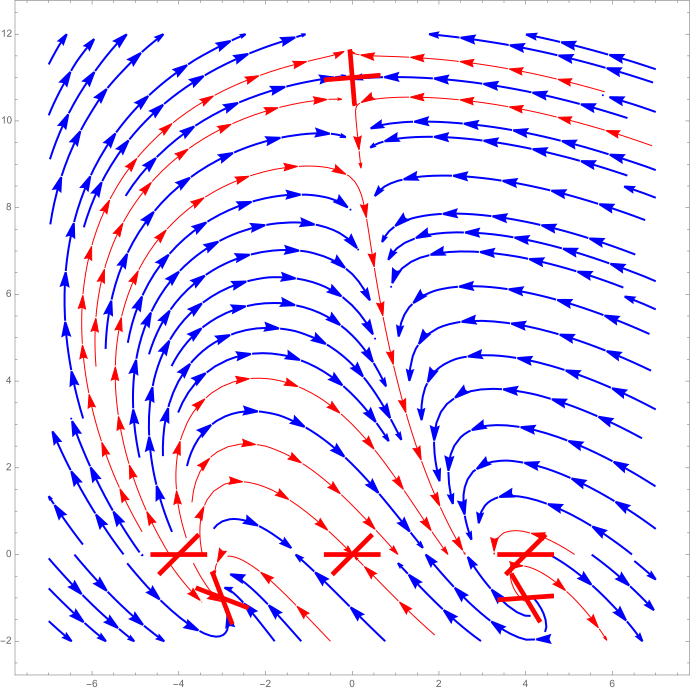
\includegraphics[width=0.7\textwidth]{additional/Stability/Points/Example2Sol.pdf}
			\caption{Фазовое пространство решения}
			\label{Stability:Example2Sol}
		\end{figure}

	% \pagebreak
		\subsection{Задачи}

	Найти и классифицировать точки покоя для следующих систем дифференциальных уравнений со степенными функциями:
	\begin{multicols}{2}
		\begin{enumtasks}
			
			\label{stability_points:types_poly1}
			\item \( \dot{x} = x + y - 3, ~ \dot{y} = 4 x - 2 y \) % \( M_1 \pares{1, 2} \) -- седловая точка
			\item \( \dot{x} = - 2x - 4y, ~ \dot{y} = - x - 2y \) % \( M_1 \pares{2C, -C} \) -- сходящееся семейство параллельных прямых
			\item \( \dot{x} = x - 2y + 6, ~ \dot{y} = 2x - 2y + 8 \) % \( M_1 \pares{-2, 2} \) -- устойчивый фокус
			\item \( \dot{x} = 6 - x - y, ~ \dot{y} = 3x \pares{2 - y} + 3 y \) % \( M_1 \pares{3, 3} \) -- устойчивый узел
			\item \( \dot{x} = 7y - 2xy + 1, ~ \dot{y} = 4y - x \) % \( M_1 \pares{4, 1} \) -- седловая точка
			\item \( \dot{x} = 1 - xy, ~ \dot{y} = x \pares{y - 1}^2 + x - y^2 \) % \( M_1 \pares{1, 1} \) -- устойчивый фокус
			\item \( \dot{x} = 2xy - 10y - 8, ~ \dot{y} = 2xy - 9y - 4 \) % \( M_1 \pares{4, -4} \) -- седловая точка
			\item \( \dot{x} = 8y - x \pares{3y - 4}, ~ \dot{y} = x \pares{y + 2} + 8 \) % \( M_1 \pares{4, -4} \) -- неустойчивый узел
			\item \( \dot{x} = y^2 \pares{x + 1} - y + 1, ~ \dot{y} = 2x - 4xy - 2 y \) % \( M_1 \pares{-1, 1} \) -- расходящееся семейство параллельных прямых
			\item \( \dot{x} = x + y - xy \pares{x + 1}, ~ \dot{y} = - x - y \) % \( M_1 \pares{-1, 1} \) -- седловая точка

		\end{enumtasks}
	\end{multicols}

	\begin{enumtasks}

		\label{stability_points:types_poly2}
		\item \( \dot{x} = 5 - x^2 - 2 y \pares{y + 1}, ~ \dot{y} = y\pares{y + 1} - x^2 - 1 \) % \( M_1 \pares{-1, 1} \) -- неустойчивый фокус, \( M_2 \pares{1, -2} \) -- устойчивый фокус
		\item \( \dot{x} = - x \pares{x + y^2}, ~ \dot{y} = 2xy \pares{x - y + 2} + 2x \) % \( M_1 \pares{0, -1} \) -- сходящееся семейство параллельных прямых, \( M_2 \pares{-1, 1} \) -- неустойчивый фокус
		\item \( \dot{x} = \pares{x - y}\pares{x + y - 3}, ~ \dot{y} = x\pares{x - 3} \pares{y + 2} - y^{2} + 3 y \) % \( M_0 \pares{0, 0} \) -- центр, \( M_1 \pares{3, 3} \) -- центр
		\item \( \dot{x} = 2x \pares{x - y^2 + 12}, ~ \dot{y} = x\pares{x - 3} \pares{y + 1} + 9 - y^2 \) % \( M_1 \pares{0, 3} \) -- устойчивый вырожденный узел, \( M_2 \pares{3, -3} \) -- неустойчивый фокус
		\item \( \dot{x} = x \pares{y - 2}^2 - 2x^2 y - 8x, ~ \dot{y} = 2x \pares{x + 2}\pares{y - 2} + 8 \) % \( M_1 \pares{-2, -2} \) -- седловая точка, \( M_2 \pares{0, 2} \) -- устойчивый дикритический узел
		\item \( \dot{x} = 2xy \pares{x + 3} - \pares{y + 1} \pares{y - 2}, ~ \dot{y} = xy \pares{2x + y + 5} - 2 x \) % \( M_1 = \pares{0, 2} \) -- неустойчивый вырожденный узел, \( M_2 \pares{-3, -1} \) -- неустойчивый узел
		
		\label{stability_points:types_poly_hard}
		\item \( \dot{x} = 6 - x \pares{x + 3} - 2 \pares{y-1}^2, ~ \dot{y} = xy \pares{2y - x - 7} - 6x - 2y \) % \( M_1 \pares{-2, 3} \) -- устойчивый узел, \( M_2 \pares{-1, -1} \) -- седловая точка
		\itemstar \( \dot{x} = \pares{x + 2y}^2 - 2y^2 + 4xy + 2x - 4y, ~ \dot{y} = x y^2 - \pares{x + y}^2 - 2 x + 2 y \) % \( M_1 \pares{0, 2} \) -- центр, \( M_2 \pares{-2, 0} \) -- неустойчивый фокус
		\itemstar \( \dot{x} = x \pares{2x - 5y - y^2 - 8}, ~ \dot{y} = x\pares{x - 1} - 2 y \pares{y + 5} - 12 \) % \( M_1 \pares{1, -3} \) -- неустойчивый узел, \( M_2 \pares{0, -2} \) -- устойчивый вырожденный узел
		\itemstar \( \dot{x} = \pares{x - 1}^2 - 2xy \pares{y + 2} - 2 \pares{y + 1}^2 - 2, ~ \dot{y} = - y\pares{x - 1}^2 - 2y^2 \) % \( M_1 \pares{3, -2} \) -- седловая точка, \( M_2 \pares{-1, 0} \) -- устойчивый дикритический узел

	\end{enumtasks}

	Найти и классифицировать точки покоя для следующих систем дифференциальных уравнений:
	\begin{multicols}{2}
		\begin{enumtasks}

			\label{stability_points:types_general}
			\item \( \dot{x} = x \sin{y}, ~ \dot{y} = y \cos{y} \) % \( M_1 \pares{0, \frac{\pi}{2} + \pi k}, ~ k \in \mathbb{Z} \) -- седловая точка ($k \ge 0$), узел ($k \% 2 = 0$ -- устойчивый, $k \% 2 = 1$ -- неустойчивый), \( M_2 \pares{C, 0} \) -- расходящееся семейство прямых
			\item \( \dot{x} = y^2 - \pi^2, ~ \dot{y} = x^2 + \cos{y} \) % \( M_1 \pares{-1, -\pi} \) -- седловая точка, \( M_2 \pares{-1, \pi} \) -- центр, \( M_3 \pares{1, -\pi} \) -- центр, \( M_4 \pares{1, \pi} \) -- седловая точка
			\item \( \dot{x} = ye^{-x}, ~ \dot{y} = \frac{\sin{y}}{x} \) % \( M_1 \pares{C, 0}, C \neq 0 \) -- семейство параллельных прямых (сходится при $C < 0$, расходится при $C > 0$)
			\item \( \dot{x} = \sin{y} - \cos{x}, ~ \dot{y} = xy \) % \( M_1 \pares{\frac{\pi}{2} + \pi k, 0} \) -- седловая точка ($k > 0, ~ k \% 2 = 1$ или $k < 0, ~ k \% 2 = 0$), узел ($k > 0, ~ k \% 2 = 0$ -- неустойчивый, $k < 0, ~ k \% 2 = 1$ -- устойчивый)
			\item \( \dot{x} = \arctan\pares{y-x}, ~ \dot{y} = x \tan\pares{x + y} \) % \( M_0 \pares{0, 0} \) -- сходящееся семейство параллельных прямых
			\item \( \dot{x} = x \cosh{2y}, ~ \dot{y} = y \cosh\pares{y - 2x} \) % \( M_0 \pares{0, 0} \) -- неустойчивый дикритический узел
			
			\label{stability_points:types_general_hard}
			\item \( \dot{x} = y - xe^{-x}, ~ \dot{y} = y^2 - xy - 2y \) % \( M_0 \pares{0, 0} \) -- устойчивый узел
			\itemstar \( \dot{x} = \frac{2}{x^2 - y} + y, ~ \dot{y} = y^2 + \cos{\pi x} \) % \( M_1 \pares{-1, -1} \) -- седловая точка, \( M_2 \pares{1, -1} \) -- устойчивый узел
			\itemstar \( \dot{x} = \frac{\cos{x}}{y + 1}, \dot{y} = \frac{\sinh{y}}{x + 1} \) % \( M_1 \pares{\frac{\pi}{2} + \pi k, 0}, ~ k \in \mathbb{Z} \) -- седловая точка ($k > 0, ~ k \% 2 = 0$ или $k < 0, ~ k \% 2 = 1$), узел ($k < 0, ~ k \% 2 = 0$ -- устойчивый, $k > 0, ~ k \% 2 = 1$ -- неустойчивый)
			\itemstar \( \dot{x} = \frac{x}{y} - \frac{y}{x}, ~ \dot{y} = \sin\pares{x + y} \) % \( M_1 \pares{\pi k, \pi k}, ~ k \in \mathbb{Z} \setminus \braces{0} \) -- сходящееся семейство параллельных прямых

		\end{enumtasks}
	\end{multicols}
		\pagebreak

		%-----------------------------------------------------------------------------------------------------------
		%===========================================================================================================
		%-----------------------------------------------------------------------------------------------------------

		\section{Критерий устойчивости уравнений с постоянными коэффициентами}

	В данном разделе мы будем рассматривать критерий Рауса-Гурвица об устойчивости линейных уравнений $n$-го порядка с постоянными коэффициентами. Согласно условиям, решение линейного уравнения с постоянными коэффициентами является устойчивым, если вещественные части корней соответствующего характеристического полинома отрицательны. Необходимым условием является положительность коэффициентов уравнения.

	Рассматривать будем линейное уравнение следующего вида:
	\[ a_0 y^{(n)} + a_1 y^{(n-1)} + \cdots + a_{n-1} y' + a_n y = 0, ~ a_i \in \mathbb{R}, ~ a_i > 0 ~ \forall i = \overline{0, n}. \]
	Соответствующий характеристический полином имеет следующий вид:
	\[ P\pares{\lambda} = a_0 \lambda^n + a_1 \lambda^{n-1} + \cdots + a_{n-1} \lambda + a_n. \]
	Решение является асимптотически устойчивым, если вещественные части корней уравнения $P\pares{\lambda} = 0$ отрицательны. Для определения отрицательности корней можно воспользоваться критерием Рауса-Гурвица. Согласно критерию, необходимо, чтобы все главные миноры матрицы Гурвица были положительными. Матрица Гурвица строится по следующим правилам:
	\begin{itemize}
		\item На главной диагонали располагаются коэффициенты характеристического уравнения, начиная с $a_1$;
		\item В столбцах коэффициенты характеристического уравнения располагаются по убыванию;
		\item В ячейках, где индекс коэффициента ниже минимального или выше максимального ставятся нули.
	\end{itemize}
	По заданным правилам, матрица Гурвица выглядит следующим образом:
	\[ G = \begin{pmatrix}
		a_1 & a_3 & a_5 & \cdots & 0 & 0 \\
		a_0 & a_2 & a_4 & \cdots & 0 & 0 \\
		0 & a_1 & a_3 & \cdots & 0 & 0 \\
		\vdots & \vdots & \vdots & \ddots & \vdots & \vdots \\
		0 & 0 & 0 & \cdots & a_{n-1} & 0 \\
		0 & 0 & 0 & \cdots & a_{n-2} & a_n \\
	\end{pmatrix}. \]

	\subsection{Пример}

		Рассмотрим пример. Для следующего уравнения определить, при каких значениях параметров $a, b$ решение является асимптотически устойчивым:
		\[ y^{IV} + 2y''' + a y'' - by' + 3y = 0. \]
		Согласно необходимому условию, коэффициенты уравнения должны быть положительны. Тогда, первое необходимое условие устойчивости: $a > 0, b < 0$. Построим матрицу Гурвица:
		\[ G = \begin{pmatrix}
			2 & -b & 0 & 0 \\
			1 & a & 3 & 0 \\
			0 & 2 & -b & 0 \\
			0 & 1 & a & 3
		\end{pmatrix}. \]
		Найдем главные миноры:
		\[ M_1 = \begin{vmatrix} 2 \end{vmatrix} = 2 > 0, ~ M_2 = \begin{vmatrix} 2 & -b \\ 1 & a \end{vmatrix} = 2a + b > 0, \]
		\[ M_3 = \begin{vmatrix}  
			2 & -b & 0 \\
			1 & a & 3 \\
			0 & 2 & -b \\
		\end{vmatrix} = 2 \begin{vmatrix} a & 3 \\ 2 & -b \end{vmatrix} - \begin{vmatrix} -b & 0 \\ 2 & -b \end{vmatrix} = -2ab - 12 - b^2 > 0, \]
		\[ M_4 = \begin{vmatrix}
			2 & -b & 0 & 0 \\
			1 & a & 3 & 0 \\
			0 & 2 & -b & 0 \\
			0 & 1 & a & 3
		\end{vmatrix} = 3M_3 > 0. \]
		Согласно критерию, необходимо, чтобы все миноры были положительны. Последний минор зависит от предпоследнего, соответственно, если $M_3 > 0$, то и $M_4 > 0$. Выпишем систему неравенств:
		\[ \syst{
			&a > 0, ~ b < 0, \\
			& 2a + b > 0, \\
			&b^2 + 2ab + 12 < 0.
		} \implies \syst{
			&a > 0, ~ b < 0, \\
			&b > -2a, \\
			&b^2 + 2ab + 12 < 0.
		} \]
		Условие $b > -2a$ не противоречит условию $b < 0$ при $a > 0$, и является усиляющим. Из последнего условия найдем ограничения для $b$:
		\[ -a - \sqrt{a^2 - 12} < b < -a + \sqrt{a^2 - 12}. \]
		Для того, чтобы $b$ было вещественным, необходимо, чтобы $a \ge \sqrt{12}$ или $a \le -\sqrt{12}$ (что противоречит условию $a > 0$). Условие $a \ge \sqrt{12}$ является усиляющим. При $a \ge \sqrt{12}$, $a > \sqrt{a^2 - 12}$. Также $-2a < -a - \sqrt{a^2 - 12} < -a + \sqrt{a^2 - 12}$, что также является усиляющим условием. Объединим все сильные условия. Таким образом, решение исходной задачи является асимптотически устойчивым при:
		\[ \syst{&a \ge \sqrt{12}, \\ &-a - \sqrt{a^2 - 12} < b < -a + \sqrt{a^2 - 12},} \]
		или, что то же:
		\[ \syst{&a \ge 2\sqrt{3}, \\ &b^2 + 2ab + 12 < 0.} \]
		На плоскости $a, b$ соответствующая область выглядит таким образом:
		\begin{figure}[H]
			\centering
			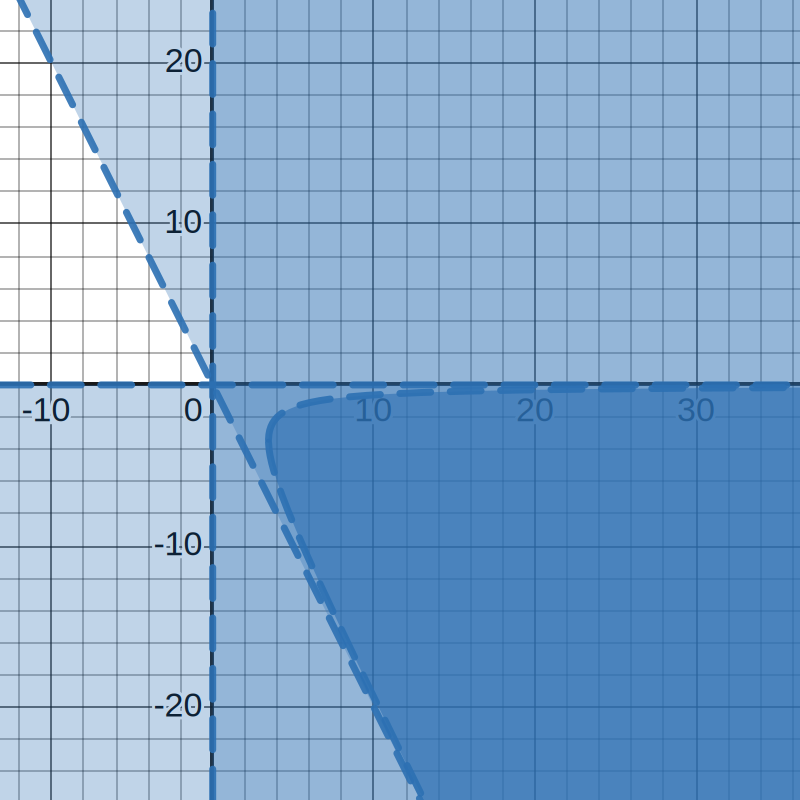
\includegraphics[width=0.5\textwidth]{additional/Stability/ranges.pdf}
			\caption{Область параметров $a, b$}
		\end{figure}

		\subsection{Задачи}

	Для следующих линейных уравнений определить, является ли решение асимптотически устойчивым:
	\begin{multicols}{2}
		\begin{enumtasks}
			
			\label{stability_hurwitz:simple_calc}
			\item \( y'' + 4y' + 2y = 0 \) % уст.
			\item \( y'' + 6y' + 8y = 0 \) % уст.
			\item \( y'' + 2y' + 5y = 0 \) % уст.
			\item \( y'' + 9y' + y = 0 \) % уст.
			\item \( y''' + 2y'' + 3y' + 2y = 0 \) % уст.
			\item \( y''' + 3y'' + 4y' + y = 0 \) % уст.
			\item \( y''' + 4y'' + y' + 4y = 0 \) % неуст.
			\item \( y''' + 5y'' + 4y' + 2y = 0 \) % уст.
			\item \( 2y''' + y'' + y' + 2y = 0 \) % неуст.
			\item \( 2y''' + 3y'' + y' + 5y = 0 \) % неуст.

			\label{stability_hurwitz:simple_calc_part2}
			\item \( 2y''' + 5y'' + 4y' + 2y = 0 \) % уст.
			\item \( 3y''' + y'' + 4y' + y = 0 \) % уст.
			\item \( 3y''' + y'' + 3y' + 5y = 0 \) % неуст.
			\item \( 3y''' + 2y'' + 3y' + 4y = 0 \) % неуст.
			\item \( y^{IV} + y''' + 4y'' + y' + 3y = 0 \) % неуст.
			\item \( y^{IV} + 3y''' + y'' + 2y' + y = 0 \) % неуст.
			\item \( y^{IV} + 5y''' + 3y'' + 4y' + 1y = 0 \) % уст.
			\item \( 2y^{IV} + 3y''' + 3y'' + 2y' + y = 0 \) % уст.
			\itemstar \( y^{V} + 2y^{IV} + y''' + y'' + 2y' + 4y = 0 \) % уст.
			\itemstar \( y^{V} + 4y^{IV} + 5y''' + 2y'' + y' + 2y = 0 \) % неуст.

		\end{enumtasks}
	\end{multicols}

	Для следующих линейных уравнений определить, при каких значениях параметров $a, b$ решение является асимптотически устойчивым:
	\begin{multicols}{2}
		\begin{enumtasks}
			
			\label{stability_hurwitz:params_ab}
			\item \( y''' + 5y'' + 4y' - ay = 0 \) % \( -20 < a < 0 \)
			\item \( ay''' + y'' + 5y' + 5y = 0 \) % \( 0 < a < 1 \)
			\item \( y''' - ay'' + 3y' + 5y = 0 \) % \( 3a + 5 < 0 \)
			\item \( 2y''' + 2y'' + ay' + y = 0 \) % \( a > 1 \)
			\item \( ay''' + 2y'' + by' + 3y = 0 \) % \( a > 0, ~ 2b > 3a \)
			\item \( y''' + ay'' - by' + 2y = 0 \) % неуст.
			\item \( y''' + 5y'' - ay' - by = 0 \) % \( b < 0, ~ 5a < b \)
			\item \( 2y''' + ay'' + 2y' + by = 0 \) % \( b > 0, ~ a > b \)
			\item \( ay''' + 2y'' + 3y' - by = 0 \) % \( a < 0, ~ b < 0, ~ ab + 6 > 0 \)
			\item \( 3y''' - ay'' + by' + 3y = 0 \) % \( a < 0, ~ b > 0, ~ ab + 9 < 0 \)
			
			\label{stability_hurwitz:params_ab_part2}
			\item \( 5y''' - ay'' + by' + 2y = 0 \) % \( a < 0, ~ ab + 10 < 0 \)
			\item \( 4y''' + ay'' + 2y' - by = 0 \) % \( b < 0, ~ a > -2b \)
			\item \( y^{IV} + y''' - ay'' + 3y' - by = 0 \) % \( b < 0, ~ 3a - b + 9 < 0 \)
			\item \( y^{IV} + 5y''' + y'' - ay' + by = 0 \) % \( b > 0, ~ a^2 + 5a + 25b < 0 \)
			\item \( y^{IV} + 2y''' + ay'' + 3y' + by = 0 \) % \( b > 0, ~ 2a > 3, ~ 6a - 4b - 9 > 0 \)
			\item \( ay^{IV} + 2y''' + 3y'' + by' + y = 0 \) % \( a > 0, ~ 4 - 6b + ab^2 < 0 \)
			\item \( y^{V} + 4y^{IV} + y''' + 4y'' + ay' - by = 0 \) % неуст.
			\item \( y^{V} - ay^{IV} + 2y''' + y'' + 2y' + by = 0 \) % \( 2a < -1, ~ 2a^2 + 2a + 1 + ab < 0 \)
			\itemstar \( 3y^{V} + 5y^{IV} + 5y''' + ay'' + by' + 5y = 0 \) % неуст.
			\itemstar \( ay^{V} + y^{IV} + 3y''' + by'' + 5y' + 5y = 0 \) % \( a > 0, 14 - 10a + 5a^2 - 3b - 3 ab + a b^2 < 0 \)

		\end{enumtasks}
	\end{multicols}
		\pagebreak

	%---------------------------------------------------------------------------------------------------------------
	%===============================================================================================================
	%---------------------------------------------------------------------------------------------------------------

	\newpart{Краевые задачи.}

		%-----------------------------------------------------------------------------------------------------------
		%===========================================================================================================
		%-----------------------------------------------------------------------------------------------------------

		\section{Краевые задачи, метод подстановки}

	В данном разделе будем рассматривать некоторые частные случаи краевых задач для обыкновенных дифференциальных уравнений.

	Введем понятие краевой задачи для обыкновенного дифференциального уравнения в общем случае. Рассмотрим уравнение на интервале следующего вида:
	\[ F \pares{x, y, y', \dots, y^{(n)}} = 0, ~ x \in \pares{x_0, x_l}. \]
	Краевыми условиями на функцию $y$ данного уравнения называется совокупность следующих дифференциальных операторов $(n-1)$-го порядка в точках $x_0$ и $x_l$:
	\[ B_i^{(n-1)} \bracks{y}\pares{x_0, x_l} = 0, ~ i = \overline{1, n}. \]
	Частный случай линейных краевых условий имеет следующий вид:
	\[ \sum_{j = 1}^{n} \pares{a_{ij} \cdot y^{(j-1)}\pares{x_0} + b_{ij} \cdot y^{(j-1)} \pares{x_l}} = c_i, i = \overline{1, n}, \]
	где \( a_{ij}, ~ b_{ij}, ~ c_i - \const ~ \forall i, j = \overline{1, n} \).
	
	Задача, содержащаяя в себе уравнение $n$-го порядка и $n$-соответствующих краевых условий называется краевой задачей. Рассматривать будем частные случаи краевых задач для уравнений второго порядка. Их классификацию будем проводить на основе следующих характеристик:
	\begin{enumerate}
		\item Условия вида \( y\pares{x_0} = y_0, ~ y\pares{x_l} = y_l \) называются краевыми условиями первого рода (условия Дирихле);
		\item Условия вида \( y'\pares{x_0} = y_0, ~ y'\pares{x_l} = y_l \) называются краевыми условиями второго рода (условия Неймана);
		\item Условия вида \( a_{11} y\pares{x_0} + a_{12} y'\pares{x_0} = y_0, ~ a_{21} y\pares{x_l} + a_{22} y'\pares{x_l} = y_l \), при условии \( a_{11}^2 + a_{12}^2 \neq 0, ~ a_{21}^2 + a_{22}^2 \neq 0 \) называются краевыми условиями третьего рода (смешанные краевые условия, условия Робена).
	\end{enumerate}
	Краевые условия называются однородными, если $y_0 = y_l = 0$.

	Рассмотрим линейное обыкновенное дифференциальное уравнение второго порядка:
	\[ y'' + p_1 \pares{x} \cdot y' + p_2 \pares{x} \cdot y = f(x), ~ x \in \pares{x_0, x_l}. \]

	Классическим решение краевой задачи Дирихле для данного уравнения будем называть такую функцию $y \pares{x} \in C^{2} \pares{x_0, x_l} \cap C\bracks{x_0, x_l}$, удовлетворяющую одновременно и уравнению и краевым условиям.

	Классическим решение краевой задачи Неймана и смешанной краевой задачи для данного уравнения будем называть такую функцию $y \pares{x} \in C^{2} \pares{x_0, x_l} \cap C^{1} \bracks{x_0, x_l}$, удовлетворяющую одновременно и уравнению и краевым условиям.

	Решение рассматриваемых в разделе можно проводить с помощью метода подстановки. Суть метода заключается в том, чтобы найти сначала общее решение уравнения, а затем, подставляя известные значения из краевыех условий, построить решение, удовлетворяющее краевой задаче.

	\subsection{Примеры}

		\begin{enumerate}
			\item Рассмотрим следующую краевую задачу для нелинейного обыкновенного дифференциального уравнения второго порядка:
				\[ \syst{
					&y'' \pares{x - \cos{y}} + 2y' + y'^2 \sin{y} = 0; \\ 
					&y\pares{0} = \pi, ~ y'\pares{1} + y\pares{1} = y'\pares{1} \cos{y\pares{1}}.
				} \]

				Представленное уравнение является уравнением с полной второй производной:
				\[ \pares{xy - \sin{y}}'' = 0, \]
				отсюда общее решение уравнения принимает вид:
				\[ xy - \sin{y} = C_1 x + C_2. \]
				Подставим первое краевое условие:
				\[ 0 \cdot \pi - \sin{\pi} = C_1 \cdot 0 + C_2 \implies C_2 = 0. \]
				Так как второе краевое условие не является линейным, но при этом в нем присутствует значение производной в точке, продифференцируем решение:
				\[ xy' + y - y' \cos{y} = C_1. \]
				Подставим $x = 1$ в это выражение, получим:
				\[ y' \pares{1} + y \pares{1} - y' \pares{1} \cos{y\pares{1}} = C_1. \]
				Данное выражение в точности повторит второе краевое условие, если $C_1 = 0$. Тогда общее решение краевой задачи принимает следующий вид:
				\[ xy = \sin{y}. \]

			\item Рассмотрим неоднородную смешанную краевую задачу для линейного неоднородного обыкновенного дифференциального уравнения второго порядка:
				\[ \syst{
					&y'' \pares{x^2 + 1} - 2xy' + 2y = 2; \\
					&y \pares{0} + y' \pares{0} = 0, ~ y' \pares{1} - y \pares{1} = 1.
				} \]
				Для однородного уравнения первое частное решение нетрудно подобрать: $y_{h_1} = x$. Построим общее однородное решение с помощью понижения порядка в линейном уравнении:
				\[ y = ux, ~ u = u \pares{x} \implies u'' x \cdot \pares{x^2 + 1} + 2u' = 0 \implies u' = C_1 \cdot \pares{1 + \frac{1}{x^2}} \implies u = C_1 \pares{x - \frac{1}{x}} + C_2. \]
				и общее однородное решение принимает вид:
				\[ y = C_1 \pares{x^2 - 1} + C_2 x. \]
				По виду уравнения нетрудно подобрать частное неоднородное решение:
				\[ y_{p} = 1. \]
				Тогда общее решение исходного уравнения принимает вид:
				\[ y = C_1 \pares{x^2 - 1} + C_2 x + 1. \]
				Для подстановки краевых условий, найдем производную от решения:
				\[ y' = 2 C_1 x + C_2. \]
				Согласно методу подстановки, составим систему уравнений для нахождения значений произвольных постоянных:
				\[ \syst{
					& \pares{- C_1 + 1} + \pares{C_2} = 0, \\
					& \pares{2C_1 + C_2} - \pares{C_2 + 1} = 1;  
				} \implies \syst{
					& C_1 - C_2 = 1, \\ &C_1 = 1;
				} \]
				из чего следует $C_1 = 1, C_2 = 0$. Тогда общее решение краевой задачи имеет следующий вид:
				\[ y = x^2. \]
				
		\end{enumerate}

	% \pagebreak

		\subsection{Задачи}

	Построить решение следующих краевых задач для линейных уравнений с постоянными коэффициентами:
	\begin{multicols}{2}
		\begin{enumtasks}

			\label{bvp_bvp:constcoeffs_simple}
			\item \( y'' = 0, ~ y(0) = 0, ~ y(1) = 0 \)		% y = 0
			\item \( y'' = 0, ~ y(0) = 0, ~ y(1) = 1 \)		% y = x
			\item \( y'' - y' = 0, ~ y(0) = 0, ~ y \pares{\ln{2}} = 1 \)		% y = e^{x} -1
			\item \( y'' - 3 y' + 2 y = 0, ~ y(0) = 1, ~ y \pares{\ln{2}} = 0 \)		% y = 2 \cdot e^{x} - e^{2 x}
			\item \( y'' - 4 y' + 3 y = 0, ~ y(0) = 2, ~ y \pares{\ln{2}} = 10 \)		% y = e^{3 x} + e^{x}
			\item \( y'' - y' - 2 y = 0, ~ y(0) = -2, ~ y \pares{\ln{3}} = 8 \)		% y = e^{2 x} -3 \cdot e^{- x}
			\item \( y'' - y' - 6 y = 0, ~ y(0) = -8, ~ y \pares{\ln{3}} = 26 \)		% y = e^{3 x} -9 \cdot e^{- 2 x}
			\item \( y'' - 4 y' + 4 y = 0, ~ y(0) = 1, ~ y(1) = 0 \)		% y = e^{2 x} - x e^{2 x}
			\item \( y'' - y = 0, ~ y(0) = -4, ~ y \pares{\ln{5}} = 4 \)		% y = e^{x} -5 \cdot e^{- x}
			\item \( y'' - 4 y = 0, ~ y(0) = -2, ~ y \pares{\ln{2}} = 7 \)		% y = 2 \cdot e^{2 x} -4 \cdot e^{- 2 x}
			\item \( y'' + y = 0, ~ y(0) = 1, ~ y \pares{\frac{\pi}{2}} = 0 \)		% y = \cos{x}
			\item \( y'' + 4 y = 0, ~ y(0) = 2, ~ y \pares{\frac{\pi}{3}} = -1 \)		% y = 2 \cdot \cos{2 x}
			\item \( y'' - 2 y' + 2 y = 0, ~ y(0) = 2, ~ y \pares{\pi} = - 2 e^{\pi} \)		% y = 2 \cdot e^{x} \cos{x} + 2 \cdot e^{x} \sin{x}
			\item \( y'' - 2 y' + 5 y = 0, ~ y(0) = 1, ~ y \pares{\pi} = e^{\pi} \)		% y = e^{x} \cos{2 x} + e^{x} \sin{2 x}
			\item \( y'' = 2, ~ y'(0) = -2, ~ y(1) = 0 \)		% y = 1 -2 \cdot x + x^{2}
			
		\end{enumtasks}
	\end{multicols}

	\begin{enumtasks}

		\label{bvp_bvp:constcoeffs_nonhmg}
		\item \( y'' - y' = -1, ~ y(-1) = e^{-1} - 1, ~ y'(1) = 1 + e \)		% y = -2 + e^{x} + x + 2
		\item \( y'' - y = 2 e^{x}, ~ y(0) = -1, ~ y' \pares{\ln{2}} = \ln{4} + 5 \)		% y = e^{x} -2 \cdot e^{- x} + x e^{x}
		\item \( y'' - 2 y' + 2 y = 2 - \sin{x} + 2 \cos{x}, ~ y'(-1) = y'(1) = - \cos{1} \)		% y = 1 - \sin{x}
		\itemstar \( y'' + 4 y = 20 e^{4 x}, ~ 2 y(0) - y'(0) = -4, ~ y \pares{\frac{\pi}{4}} - y' \pares{\frac{\pi}{4}} = 1 - 3 e^{\pi} \)		% y = \sin{2 x} + e^{4 x}
		\itemstar \( y'' + 4 y = \frac{2\pi^2}{x^3} \cdot \pares{2x^2 + 1}, ~ y \pares{-\pi} + y' \pares{-\pi} = - \pi - 1, ~ y \pares{\pi} - y' \pares{\pi} = \frac{4}{\pi} + 1 + \pi \)		% y = 2/pi \cdot \cos{2 x} -1/pi \cdot \sin{2 x} + \frac{\pi^2}{x}

	\end{enumtasks}

	Построить решение следующих краевых задач для линейных уравнений с переменными коэффициентами:
	\begin{enumtasks}

		\label{bvp_bvp:linear}
		\item \( x^2 y'' + xy' - y = 0, ~ y(-1) = -2, ~ y(1) = 2 \) % y = x + \frac{1}{x}
		\item \( y'' x \pares{x - 2} + 2y = 2y' \pares{x - 1}, ~ y(0) = 1, ~ y(1) = 1 \) % y = x^2 - x + 1
		\item \( y'' \pares{x - 1} - xy' + y = 0, ~ y(0) = 1, ~ y' \pares{\ln{2}} = 1 \) % y = - x + e^{x}
		\item \( y'' \pares{2x - 1} - 2y' = y \pares{2x - 3}, ~ y'(0) = 2, ~ y \pares{\ln{3}} = \ln{3} - 3 \) % y = 3 x e^{- x} - e^{x}
		\item \( y'' + 2 \cos{x} = y' \tan{x} + y \sec^2{x}, ~ y(0) = 0, ~ y'\pares{\pi} = 4 \) % y = \cos{x} + 4 \tan{x} - \sec{x}
		\item \( y'' \pares{2x \cot{2x} - 1}= 4 \pares{y - xy' - 1}, ~ y'(0) = 1, ~ y\pares{\pi} = 1 - \pi \) % y = \sin{2x} - x + 1
		
		\label{bvp_bvp:linear_hard}
		\itemstar \( y'' \pares{x - 1} - xy' + y = 2xe^{-x}, ~ y(0) + y'(1) = 1 + 2 \sinh{1}, ~ y(1) - y'(1) = \frac{2}{e} \) % y = e^{x} + e^{- x} - x
		\itemstar \( x y'' \pares{x \ln{x} + 1} + y' \pares{x^2 \ln{x} + 1} = \pares{y - 1} \pares{x - 1}, ~ y(1) + y'(1) = 3, ~ y(1) - y'(2) = \frac{1 + e}{e^2} \) % y = 2 \ln{x} + 1 + e^{- x}
		\itemstar \( \syst{&\pares{x^2 + 1}^2 \pares{y'' - 2} \arctan{x} + x \pares{x^2 + 1} \pares{y'' - 2} + 2xy = 2x^2 \pares{y' - x}, \\ &y(0) + 2y(1) = \pi + 4, ~ y'(1) - y'(0) = 1} \) % y = x^{2} + x + 2 \arctan{x}
		\itemstar \( \syst{&x^2 \ln{x} \pares{y'' - y'} - x \ln{x} \pares{y'' - y} - xy'' + y' + \pares{x - 1} y = x^2 - x + 1, \\ &y'(1) - y(1) = 2, ~ 2y'(1) + 2y'(2) - y(2) = 2e + e^2 + 10} \) % y = 2 x \ln{x} + x + e^{x}

	\end{enumtasks}

	Классифицировать следующие нелинейные краевые задачи, и построить решение с помощью метода подстановки:
	\begin{enumtasks}

		\label{bvp_bvp:nonlinear}
		\item \( xyy'' + xy'^2 + yy' = 0, ~ y(1) = 0, ~ y(2) \cdot y'(2) = 1 \) % y^2 = 4 \ln{x}
		\item \( y'' - y'^2 = \frac{y'}{x + 1}, ~ y(0) - y'(0) = 2, ~ y'(1) = -1 \) % e^{- y} = \pares{x + 1}^2
		\item \( y'^2 \pares{y \tanh{y} + 2} = \pares{y' - y''} \cdot \pares{y + \tanh{y}}, ~ y(0) = 0, ~ y(\sinh{1}) = 1 \) % y \sinh{y} = x
		\item \( x \pares{2 \ln{x} - 1} \cdot \pares{y'^2 - yy''} = yy' \cdot \pares{6 \ln{x} - 5}, ~ y(1) = e, ~ y(e) = 1 \) % x^2 \ln{y} = x^2 -  e^2 \ln{x}
		\item \( 2yy' \pares{\cos^2{x} + 1} + \pares{yy'' + y'^2} \sin{2x} = 0, ~ y(0) = 0, ~ y \pares{\frac{\pi}{2}} = 1 \) % y = 1 
		\item \( y'' + 2y'^2 \tan{y} = 2y' \tan{x}, ~ y\pares{\frac{\pi}{4}} = \frac{\pi}{4}, ~ y'(\pi) = 0 \) % \tan{y} = C_1 \tan{x} + C_2
		
		\label{bvp_bvp:nonlinear_hard}
		\item \( y'' + y'^2 - y' = \frac{y'}{x + 1}, ~ y'(-1) - y(-1) = 1, ~ y(0) + y'(0) = e - 1 \) % e^y = (e - 1) \cdot x e^x + 1
		\item \( xy'' + y' = xy'^2 \tan{y}, ~ y'(1) \cdot \cos{y(1)} = -1, ~ y(e) = 0 \) % \sin{y} = 1 - \ln{x}
		\itemstar \( 2xyy' + \pares{x^2 + 1} \cdot \pares{yy'' + y'^2} = 0, ~ y(0) \cdot y'(0) = 2, ~ y^2(1) + 2y(0) \cdot y'(1) = \pi \) % y^2 = 4 \arctan{x} - 2
		\itemdstar \( xy'^2 + xy'' + 2x = y' \pares{3x - 2} + 3, ~ y(1) = 1, ~ y(e) = e - 1 \) % x e^{y - x} = 1

	\end{enumtasks}


		\pagebreak

		%-----------------------------------------------------------------------------------------------------------
		%===========================================================================================================
		%-----------------------------------------------------------------------------------------------------------

		\section{Функции Грина}

	В данном разделе рассмотрим интегральные формулы Грина и функции Грина для решения краевых задач для линейных уравнений второго порядка.

	Введем линейный дифференциальный оператор второго порядка по следующему правилу:
	\[ L[u] = \difft{}{x} \bracks{ p(x) \cdot \difft{u}{x} } - q(x) \cdot u, ~ u = u(x) \]

	Рассмотрим краевую задачу для следующего линейного дифференциального уравнения второго порядка:
	\[ L[u] = f(x), ~ x \in \pares{x_0, x_l} \]
	с однородными краевыми условиями Дирихле:
	\[ u(x_0) = u(x_l) = 0. \]
	Введем такую функцию $v \in C^2[x_0, x_l]$, удовлетворяющую однородным условиям Дирихле:
	\[ v(x_0) = v(x_l) = 0, \]
	затем домножим исходное уравнение на данную функцию, и проинтегрируем по области $D = [x_0, x_l]$:
	\[ \int\limits_{x_0}^{x_l} L[u] \cdot v ~ dx = \int\limits_{x_0}^{x_l} f \cdot v ~ dx. \]
	Раскроем линейный оператор:
	\[ \int\limits_{x_0}^{x_l} \difft{}{x} \bracks{p \cdot \difft{u}{x}} \cdot v ~ dx - \int\limits_{x_0}^{x_l} q \cdot u \cdot v ~ dx = \int\limits_{x_0}^{x_l} f \cdot v ~ dx. \]
	Для первого слагаемого воспользуемся формулой интегрирования по частям:
	\[ \int\limits_{x_0}^{x_l} \difft{}{x} \bracks{p \cdot \difft{u}{x}} \cdot v ~ dx = p \cdot v \cdot \difft{u}{x} \at_{x_0}^{x_l} - \int\limits_{x_0}^{x_l} p \cdot \difft{u}{x} \cdot \difft{v}{x} ~ dx. \]
	Из условия, что функция $v$ удовлетворяет однородным условиям Дирихле, следует:
	\[ \int\limits_{x_0}^{x_l} \difft{}{x} \bracks{p \cdot \difft{u}{x}} \cdot v ~ dx = - \int\limits_{x_0}^{x_l} p \cdot \difft{u}{x} \cdot \difft{v}{x} ~ dx. \]
	Введем скалярное произведение следующим образом:
	\[ \pares{u, v} = \int\limits_{x_0}^{x_l} u(x) \cdot v(x) ~ dx, \]
	тогда исходная задача принимает следующий вид:
	\[ -\pares{p \cdot u', v'} - \pares{q \cdot u, v} = \pares{f, v}, \]
	что является частным случаем первой формулы Грина, а исходная краевая задача сведена к интегральной.

	\vspace{10pt}

	Теперь рассмотрим способы сведения линейных краевых задач с неоднородными краевыми условиями к неоднородным линейным краевым задачам с однородными краевыми условиями. Снова рассмотрим уравнение
	\[ L[y] = f(x), ~ x \in \pares{x_0, x_l} \]
	с неоднородными смешанными краевыми условиями:
	\[ a_{11} y(x_0) + a_{12} y'(x_0) = y_0, ~ a_{21} y(x_l) + a_{22} y'(x_l) = y_l. \]
	Так как представленное уравнение является линейным, то выполняется принцип суперпозиции:
	\[ y = u + v. \]
	Пусть функция $v$ удовлетворяет только неоднородным краевым условиям, тогда функция $u$ должна удовлетворять, соответственно, однородным краевым условиям, и новому уравнению. Построим новую краевую задачу из этих условий:
	\[ L[u] + L[v] = f(x), ~ x \in \pares{x_0, x_l}, \]
	\[ a_{11} u(x_0) + a_{12} u'(x_0) = 0, ~ a_{21} u(x_l) + a_{22} u'(x_l) = 0, \]
	\[ a_{11} v(x_0) + a_{12} v'(x_0) = y_0, ~ a_{21} v(x_l) + a_{22} v'(x_l) = y_l. \]
	Положим, что функцию $v$ можно подобрать согласно краевым условиям, тогда краевая задача сводится к задаче с однородными краевыми условиями относительно новой неизвестной функции $u$.

	Подбирать функцию $v$ можно различными способами. Например, пусть $v$ -- некоторая квадратичная функция с неопределенными коэффициентами: $v = Ax^2 + Bx + C$. Подставляя в краевые условия, можно подобрать значения коэффициентов $A, B, C$:
	\[ \syst{
		&a_{11} \pares{A x_0^2 + B x_0 + C} + a_{12} \pares{2A x_0 + B} = y_0, \\
		&a_{21} \pares{A x_l^2 + B x_l + C} + a_{22} \pares{2A x_l + B} = y_l, \\
	} \] 
	Представленная система является линейной системой алгебраических уравнений из двух уравнений и трех неизвестных. Из этой системы можно получить любой набор коэффициентов $A, B, C$, на основе которых построить такую функцию $v$, которая будет удовлетворять краевым условиям. Так как функция $v$ известна, то и известно значение выражения $L[v]$. Пусть $g(x) = f(x) - L[v]$. Тогда краевая задача принимает следующий вид:
	\[ L[u] = g(x), ~ x \in \pares{x_0, x_l}, \]
	\[ a_{11} u(x_0) + a_{12} u'(x_0) = 0, ~ a_{21} u(x_l) + a_{22} u'(x_l) = 0. \]
	Решая данную задачу, и подставляя известное значение функции $v$, получим решение исходной краевой задачи.

	\vspace{10pt}

	Рассмотрим линейный неоднородный дифференциальный оператор с однородными смешанными краевыми условиями:
	\[ L[u] = f(x), ~ x \in \pares{x_0, x_l}, ~ L[u] = \difft{}{x} \bracks{p \cdot \difft{u}{x}} - q \cdot u, \]
	\[ B_0[u] = a_{11} u(x_0) + a_{12} u'(x_0) = 0, ~ B_l[u] = a_{21} u(x_l) + a_{22} u'(x_l) = 0. \]
	Функцией Грина данной краевой задачи называется такая функция $G(x, t)$, удовлетворяющая следующим условиям:
	\begin{enumerate}
		\item $G(x, t) \in \pares{C^2 \pares{x_0, x_l} \cap C\bracks{x_0, x_l}} \times \pares{C^1 \pares{x_0, x_l} \cap C\bracks{x_0, x_l}}$ -- непрерывна на квадрате, дважды дифференцируема по $x$, и дифференцируема один раз по $t$;
		\item $L_x \bracks{G(x, t)} = \delta\pares{x - t} = \syst{& 0: x \neq t \\ & 1: x = t }$ -- удовлетворяет однородному уравнению, когда $x \neq t$, и оператор равен $1$ при $x = t$;
		\item $B_0\bracks{G(x, t)} = B_l\bracks{G(x, t)} = 0$ -- удовлетворяет однородным краевым условиям по переменной $x$;
		\item $\lim\limits_{\varepsilon \to 0} \dpart{G}{x} \at_{x = t - \varepsilon}^{x = t + \varepsilon} = \frac{1}{p(t)}$ -- производная функции терпит разрыв первого рода со скачком в точке $x = t$.
	\end{enumerate}

	Функция Грина является обратным оператором для исходной краевой задачи. Решение можно записать в следующем виде:
	\[ u(x) = \int\limits_{x_0}^{x_l} G(x, t) \cdot f(t) ~ dt. \]
	Справедливость данного выражения можно доказать следующим образом:
	\[ L[u] = L_x\bracks{\int\limits_{x_0}^{x_l} G(x, t) \cdot f(t) ~ dt} = \int\limits_{x_0}^{x_l} L_x[G(x, t)] \cdot f(t) ~ dt = \int\limits_{x_0}^{x_l} \delta(x - t) \cdot f(t) ~ dt = f(x). \]
	Такая функция удовлетворяет уравнению. Краевые условия выполняются согласно условиям, наложенным на функцию $G$.

	Рассмотрим построение функции Грина. Положим следующее уравнение:
	\[ L[G(x, t)] = 0, ~ x \neq t. \]
	Рассмотрим следующие две области:
	\[ I_0(t) = [x_0, t), ~ I_l(t) = (t, x_l]. \]
	Пусть $u_0, u_l$ -- линейно-независимые частные решения однородного уравнения, при условии, что:
	\[ B_0[u_0] = 0, ~ B_l[u_l] = 0. \]
	Тогда пусть функция Грина принимает следующий вид:
	\[ G(x, t) = \syst{
		& C_1(t) \cdot u_0(x), ~ x \in I_0(t), \\
		& C_2(t) \cdot u_l(x), ~ x \in I_l(t).
	} \]
	Удовлетворим условие непрерывности функции в точке $x = t$:
	\[ \lim\limits_{\varepsilon \to 0} G(t - \varepsilon, t) = \lim\limits_{\varepsilon \to 0} G(t + \varepsilon, t), \]
	из чего следует:
	\[ C_1(t) \cdot u_0(t) = C_2(t) \cdot u_l(t). \]
	Затем удовлетворим условие разрывности производной функции в точке $x = t$:
	\[ \lim\limits_{\varepsilon \to 0} \dpart{G}{x} \at_{x = t - \varepsilon}^{x = t + \varepsilon} = \frac{1}{p(t)}, \]
	из чего следует:
	\[ C_2(t) \cdot u_l'(t) - C_1(t) \cdot u_0'(t) = \frac{1}{p(t)}. \]
	Рассматривая систему, построенную на двух данных условиях, возможно найти неизвестные функции $C_1(t)$ и $C_2(t)$. Тогда возможно определить единственную функцию Грина на основе конкретных функций $u_0$ и $u_l$.

	\subsection{Примеры}

		\begin{enumerate}

			\item Построим интегральную форму следующей краевой задачи:
				\[ y'' + y' - 2y = 10e^{-x} \cos{x}, ~ y(0) = 1, ~ y(\ln{2}) = -1. \]
				Введем функцию $v$, удовлетворяющую однородным условиям Дирихле:
				\[ v(0) = v(\ln{2}) = 0. \]
				Найдем функции $p(x)$ и $q(x)$. Домножим исходное уравнение на некоторой неизвестный интегрирующий множитель $\mu(x)$. Соответствующее уравнение для функций $p$ и $q$ можно найти из следующего соотношения:
				\[ \mu \cdot \pares{y'' + y' - 2y} = \difft{}{x} \bracks{p \cdot y'} - q \cdot y \]
				Раскрываем скобки, получим:
				\[ y'' \mu + y' \mu - 2y \mu = py'' + p'y' - qy, \]
				отсюда:
				\[ p = \mu, ~ p' = \mu, ~ q = 2 \mu. \]
				Найдем $p$:
				\[ p' = p \implies p = C e^{x}, \text{ пусть } C = 1, \]
				тогда
				\[ q = 2 e^{x}. \]
				Сведем исходное уравнение к операторному виду:
				\[ L[y] = \difft{}{x} \bracks{y' e^x} - 2 y e^x = 10 \cos{x}. \]
				Домножим уравнение на функцию $v$, и проинтегрируем:
				\[ \int\limits_{0}^{\ln{2}} \difft{}{x} \bracks{y' e^x} \cdot v ~ dx - 2 \int\limits_{0}^{\ln{2}} y e^{x} \cdot v ~ dx = 10 \int\limits_{0}^{\ln{2}} \cos{x} \cdot v ~ dx. \]
				Воспользуемся формулой интегрирования по частям для первого интеграла, получим:
				\[ y' e^{x} \cdot v \at_{x = 0}^{x = \ln{2}} - \int\limits_{0}^{\ln{2}} y' e^{x} \cdot v' ~ dx - 2 \int\limits_{0}^{\ln{2}} y e^{x} \cdot v ~ dx = 10 \int\limits_{0}^{\ln{2}} \cos{x} \cdot v ~ dx. \]
				Введем скалярное произведение следующим образом:
				\[ \pares{u, v} = \int\limits_{0}^{\ln{2}} u(x) \cdot v(x) ~ dx. \]
				Упростим выражение, получим следующую интегральную форму исходной краевой задачи:
				\[ \pares{y' e^{x}, v'} + 2 \pares{y e^{x}, v} = - 10 \pares{\cos{x}, v}. \]

			\item Построим решение следующей неоднородной краевой задачи для линейного неоднородного уравнения второго порядка с переменными коэффициентами:
				\[ \syst{
					&x \pares{2x - 1} y'' + 2 \pares{x - 1} y' - 2y = 6x \pares{x - 1} + 2, \\ 
					&y(1) + y'(1) = 3, ~ 2y(2) - y'(2) = 3 
				}\]
				Решение будем строить в виде линейной комбинации двух функций:
				\[ y = u + v, \]
				где функция $v$ удовлетворяет неоднородным краевым условиям, а для функции $u$ ставится новая краевая задача. Пусть $v$ -- некоторая линейная функция: $v = Ax + B$. Найдем коэффициенты $A$ и $B$:
				\[ \syst{
					& 2A + B = 3 \\
					& 3A + 2B = 3
				} \implies A = 3, B = -3, ~ v(x) = 3\pares{x - 1}. \]
				% Подставляя значение функции $v$ в исходное уравнение, получим, что $L[v] = 0$.
				Тогда новая краевая задача принимает следующий вид:
				\[ \syst{
					&x \pares{2x - 1} \pares{u + 3x - 3}'' + 2 \pares{x - 1} \pares{u + 3x - 3}' - 2 \pares{u + 3x - 3} = 6x \pares{x - 1} + 2, \\ 
					&u(1) + u'(1) = 0, ~ 2u(2) - u'(2) = 0
				} \]
				Раскроем скобки, упростим выражение:
				\[ \syst{
					&x \pares{2x - 1} u'' + 2 \pares{x - 1} u' - 2u = 6x \pares{x - 1} + 2, \\
					&u(1) + u'(1) = 0, ~ 2u(2) - u'(2) = 0 
				}\]
				Найдем значение функций $p(x)$ и $q(x)$ домножая исходное уравнение на интегрирующий множитель $\mu(x)$:
				\[ \mu \cdot \bpares{x \pares{2x - 1} u'' + 2 \pares{x - 1} u' - 2u} = p u'' + p'u' - q u. \]
				Отсюда следует:
				\[ p = \mu \cdot x \pares{2x - 1}, ~ p' = 2\mu \cdot \pares{x - 1}, ~ q = 2\mu. \]
				Найдем $p$:
				\[ \frac{p'}{p} = \frac{2 \pares{x - 1}}{x \pares{2x - 1}} \implies p(x) = \frac{C x^2}{2x - 1}, ~ \text{пусть } C = 1, \]
				тогда
				\[ \mu(x) = \frac{x}{\pares{2x - 1}^2}, ~ q(x) = \frac{2x}{\pares{2x - 1}^2}, ~ f(x) = \frac{2x \bpares{3x \pares{x - 1} + 1}}{\pares{2x - 1}^2} \]
				Таким образом, исходное уравнение принимает следующий вид:
				\[ \difft{}{x} \bracks{ \frac{x^2}{2x - 1} \cdot u' } - \frac{2x}{\pares{2x - 1}^2} = \frac{2x \bpares{3x \pares{x - 1} + 1}}{\pares{2x - 1}^2} \]
				Найдем однородные решения исходного уравнения:
				\[ x \pares{2x - 1} u'' + 2 \pares{x - 1} u' - 2u = 0. \]
				Подберем частное решение. Пусть $u = x^n$. Подставим в уравнение:
				\[ n\pares{n - 1} \cdot x \pares{2x - 1} x^{n - 2} + 2n \pares{x - 1} \cdot x^{n-1} - 2x^n = 0. \]
				Рассчитаем коэффициенты при старших степенях $x$:
				\[ 2n \pares{n - 1} x^n + 2n x^n - 2x^n = 0 \implies n = \pm 1. \]
				Найдем частное решение в виде полинома степени $n = 1$: $u = x + a$. Подставим в уравнение:
				\[ 2 \pares{x - 1} - 2 \pares{x + a} = 0 \implies a = -1. \]
				Частное решение однородного уравнения: $u = x - 1$. Найдем второе частное решение. Положим $u = z \cdot \pares{x - 1}, ~ z = z(x)$. Подставим в уравнение:
				\[ x\pares{2x^2 - 3x + 1} z'' + 2\pares{3x^2 - 3x + 1} z' = 0. \]
				Разделяя переменные, получим:
				\[ z' = C_1 \cdot \frac{1 - 2x}{x^2 \pares{x-1}^2} \implies z = C_1 \pares{\frac{1}{x-1} - \frac{1}{x}} + C_2. \]
				Подставляя и упрощая, получим общее решение однородного уравнения:
				\[ u = C_1 \pares{x - 1} + \frac{C_2}{x} \]

				Подберем два линейно-независимых частных решения, удовлетворящих однородным краевым условиям. Для этого найдем производную функции $u$:
				\[ u' = C_1 - \frac{C_2}{x^2}. \]
				Система для двух частных решений принимает вид:
				\[ \begin{matrix}
					\syst{&u_1 = C_1 \pares{x - 1} + \frac{C_2}{x}, \\ &u_1(1) + u_1'(1) = 0.} & 
					\syst{&u_2 = C_1 \pares{x - 1} + \frac{C_2}{x}, \\ &2u_2(2) - u_2'(2) = 0.} 
				\end{matrix} \]
				Подберем значения $C_1$ и $C_2$ для функций $u_1$ и $u_2$:
				\[ u_1: C_2 + C_1 - C_2 = 0; \quad u_2: 2C_1 + C_2 - C_1 + \frac{C_2}4 = 0. \]
				Выберем следующие функции:
				\[ u_1 = \frac{1}{x}, ~ u_2 = 5 \pares{x - 1} - \frac{4}{x}. \]
				Проверим их линейную независимость:
				\[ W(x) = \begin{vmatrix} 
					\dfrac{1}{x} & 5 \pares{x - 1} - \dfrac{4}{x} \\
					-\dfrac{1}{x^2} & 5 + \dfrac{4}{x^2}
				\end{vmatrix} = \frac{5}{x^2} \pares{2x - 1} \neq 0. \]

				Построим функцию Грина:
				\[ G(x, t) = \syst{
					& \frac{C_1(t)}{x}, ~ 1 \le x < t \le 2, \\
					& C_2(t) \cdot \pares{5 \pares{x - 1} - \frac{4}{x}}, ~ 1 \le t < x \le 2.
				} \]
				Выпишем условия непрерывности и разрывности функции Грина:
				\[ \syst{
					& \frac{C_1(t)}{t} = C_2(t) \cdot \pares{5 \pares{t - 1} - \frac{4}{t}} \\
					& C_2(t) \cdot \pares{5 + \frac{4}{t^2}} + \frac{C_1(t)}{t^2} = \frac{1}{p(t)} = \frac{2t - 1}{t^2}.
				} \]
				Запишем данную систему в матричной форме относительно неизвестных $C_1(t)$ и $C_2(t)$:
				\[ \begin{pmatrix} 
					\dfrac{1}{t} & -5 \pares{t - 1} + \dfrac{4}{t} \\
					\dfrac{1}{t^2} & 5 + \dfrac{4}{t^2}
				\end{pmatrix} \begin{pmatrix} C_1(t) \\ C_2(t) \end{pmatrix} = \begin{pmatrix} 0 \\ \dfrac{2t - 1}{t^2} \end{pmatrix} \]
				Определитель матрицы коэффициентов при $C_1(t)$, $C_2(t)$ известен, и равен $W(t)$. Тогда
				\[ C_1(t) = \frac{t^2}{5\pares{2t - 1}} \cdot \pares{5 \pares{t - 1} - \frac{4}{t}} \cdot \frac{2t - 1}{t^2} = \frac{1}{5} \pares{5 \pares{t - 1} - \frac{4}{t}}, \] 
				\[ C_2(t) = \frac{t^2}{5\pares{2t - 1}} \cdot \frac{1}{t} \cdot \frac{2t - 1}{t^2} = \frac{1}{5t}. \]
				Тогда функция Грина принимает следующий вид:
				\[ G(x, t) = \syst{
					& \frac{1}{5x} \cdot \pares{5 \pares{t - 1} - \frac{4}{t}}, ~ 1 \le x < t \le 2, \\
					& \frac{1}{5t} \cdot \pares{5 \pares{x - 1} - \frac{4}{x}}, ~ 1 \le t < x \le 2.
				} \] 

				Построим решение новой краевой задачи:
				\[ u(x) = \int\limits_1^2 G(x, t) \cdot f(t) ~ dt = \int\limits_1^x G_2(x, t) \cdot f(t) ~ dt + \int\limits_x^2 G_1(x, t) \cdot f(t) ~ dt = \circledast \]
				Рассмотрим каждый интеграл отдельно:
				\[
					I_1 = \int\limits_1^x G_2(x, t) \cdot f(t) ~ dt = \frac{1}{5} \cdot \pares{5 \pares{x - 1} - \frac{4}{x}} \cdot \int\limits_1^x \frac{1}{t} \cdot \frac{2t \bpares{3t \pares{t - 1} + 1}}{\pares{2t - 1}^2} ~ dt = \star
				\]
				\[ \begin{split} 
					I'_1 &= 2 \int\limits_1^x \frac{3t \pares{t - 1} + 1}{\pares{2t - 1}^2} ~ dt = \frac{1}{2} \int\limits_1^x 3 + \frac{1}{\pares{2t - 1}^2} = \frac{3}{2} t - \frac{1}{4 \pares{2t - 1}} \at_{t = 1}^{t = x} = \\
					&= \frac{3}{2} x - \frac{1}{4 \pares{2x - 1}} - \frac{5}{4} = \frac{1}{4} \cdot \pares{6x - 5 - \frac{1}{2x - 1}};
				\end{split} \]
				\[ 
					\star = \frac{1}{20} \cdot \pares{5 \pares{x - 1} - \frac{4}{x}} \cdot \pares{6x - 5 - \frac{1}{2x - 1}} = \frac{15x^4 - 35 x^3 + 13x^2 + 11x - 4}{5x \pares{2x - 1}};
				\]

				\[ 
					I_2 = \int\limits_x^2 G_1(x, t) \cdot f(t) ~ dt = \frac{1}{5x} \cdot \int\limits_x^2 \pares{5 \pares{t - 1} - \frac{4}{t}} \cdot \frac{2t \bpares{3t \pares{t - 1} + 1}}{\pares{2t - 1}^2} ~ dt = \star
				\]
				\[ \begin{split}
					I'_2 &= \int\limits_x^2 \pares{5 \pares{t - 1} - \frac{4}{t}} \cdot \frac{2t \bpares{3t \pares{t - 1} + 1}}{\pares{2t - 1}^2} ~ dt = \int\limits_x^2 \frac{15}{2} t^2 - \frac{15}{2} t - \frac{43}{8} - \frac{21}{8 \pares{2t - 1}^2} ~ dt = \\
					&= \frac{5}{2} t^3 - \frac{15}{4} t^2 - \frac{43}{8} t + \frac{21}{16\pares{2t - 1}} \at_{t = x}^{t = 2} = -\frac{39}{8} - \frac{5}{2} x^3 + \frac{15}{4} x^2 + \frac{43}{8} x - \frac{21}{16\pares{2x - 1}} = \\
					&= -\frac{5x^4 - 10x^3 - 7x^2 + 16x - 4}{2x - 1};
				\end{split} \]
				\[ 
					\star = -\frac{5x^4 - 10x^3 - 7x^2 + 16x - 4}{5x \pares{2x - 1}};
				\]
				\[ \begin{split}
					\circledast &= \frac{15x^4 - 35 x^3 + 13x^2 + 11x - 4}{5x \pares{2x - 1}} - \frac{5x^4 - 10x^3 - 7x^2 + 16x - 4}{5x \pares{2x - 1}} = \\
					&= \frac{10x^4 - 25 x^3 + 20x^2 - 5x}{5x \pares{2x - 1}} = \frac{2x^3 - 5x^2 + 4x - 1}{2x - 1} = \pares{x-1}^2.
				\end{split} \]
				Тогда общее решение принимает вид:
				\[ y = u + v = \pares{x-1}^2 + 3 \pares{x-1} = x^2 + x - 2. \]

		\end{enumerate}

	\subsubsection*{Замечание}

		На примере видно, что функция Грина является симметричной относительно аргументов $x$ и $t$. В общем случае данная функция может быть представлена в следующем виде:
		\[ G(x, t) = \syst{
			& \frac{u_0(x) \cdot u_l(t)}{W(t) \cdot p(t)}, ~ x_0 \le x < t \le x_l, \\
			& \frac{u_0(t) \cdot u_l(x)}{W(t) \cdot p(t)}, ~ x_0 \le t < x \le x_l,
		} \]
		где $u_0, u_l$ -- частные решения, удовлетворяющие первому и второму краевым условиям, $W(t)$ -- определитель Вронского системы двух частных решений, $p(t)$ -- коэффициент при старшей производной в рассматриваемом линейном дифференциальном операторе. 

	% \pagebreak
		\subsection{Задачи}

	Свести задачу к задаче с однородными краевыми условиями, найти интегрирующий множитель и построить интегральную форму для следующих краевых задач:
	\begin{enumtasks}

		\label{bvp_green:int_factor}
		\item \( x^2 u'' + xu' - u = 0, ~ u(-1) = -1, ~ u(1) = 1 \) % u = x; \( w = x, ~ \mu = \frac{1}{x}, ~ \pares{xu', v'} + \pares{\frac{u}{x}, v} = 0 \)
		\item \( xu'' + \pares{x - 1} u' - u = -1, ~ u(0) = 0, ~ u(1) = 1 \) % u = x; \( w = x, ~ \mu = \frac{e^x}{x^2}, ~ \pares{\frac{e^x}{x} u', v'} + \pares{\frac{e^x}{x^2} u, v} = 0 \)
		\item \( \pares{2x - 1} u'' - 2u' - \pares{2x - 3} u = 3x - 2x^2 - 2, ~ u(-1) = \frac{1}{e} - 1, ~ u(1) = 1 + e \) % u = x + e^x; \( w = x + e^x, ~ \mu = \frac{1}{\pares{2x - 1}^2}, ~ \pares{\frac{u'}{2x - 1}, v'} + \pares{\frac{2x - 3}{\pares{2x - 1}^2} u, v} = 0 \)
		\item \( x^2 u'' = 2 \pares{xu' - u + 1}, ~ u(0) = 1, ~ u(1) = 1 \) % u = x^2 - x + 1; \( w = 1, ~ \mu = \frac{1}{x^4}, ~ \pares{\frac{u'}{x^2}, v'} - 2\pares{\frac{u}{x^4}, v} = -\pares{\frac{2}{x^4}, v} \)
		\item \( x \pares{x - 4} u'' - 2 \pares{x - 2} u' + 2u = - 4, ~ u(0) = 2, ~ u(1) = 1 \) % u = x^2 - 2x + 2; \( w = 2 - x, ~ \mu = \frac{1}{x^2 \pares{x - 4}^2}, ~ \pares{\frac{u'}{x\pares{x - 4}}, v'} - 2\pares{\frac{u}{x^2 \pares{x - 4}^2}, v} = 4 \pares{\frac{1}{x^2 \pares{x - 4}^2}, v} \)
		\item \( x \pares{x - 1} u'' + \pares{x + 1} u' - u = 3x^2, ~ u(-1) = 1, ~ u(1) = 3 \) % u = x^2 + x + 1; \( w = x + 2, ~ \mu = \frac{x - 1}{x^2}, ~ \pares{\frac{\pares{x-1}^2}{x} u', v'} + \pares{\frac{\pares{x-1}}{x^2} u, v} = \pares{\pares{3 + \frac{1}{x^2}} \pares{1 - x}, v} \)
		\item \( u'' - 3u' \cot{x} + \pares{3 \cosec^2{x} - 2} u = 3 \cot{x} \cosec{x}, ~ u(0) = 1, ~ u\pares{\frac{\pi}{2}} = 0 \) % u = \sin{2x} + \cos{x}; \( w = \cos{x}, ~ \mu = \cosec^3{x}, ~ \pares{u' \cosec^3{x}, v'} - \pares{\pares{2 + \cos{2x}} \cdot u \cosec^5{x}, v} = 0 \)
		\itemstar \( x \pares{x - 2} u'' - \pares{x^2 - 2} u' + 2 \pares{x - 1} u = \pares{x - 2}^2, ~ u(0) = -2, ~ u(1) = 1 - e \) % u = x^2 + x - e^x - 1; \( w = 2x - 1 - e^x, ~ \mu = \frac{e^{-x}}{x^2 \pares{x - 2}^2}, ~ \pares{\frac{e^{-x}}{x \pares{x-2}} u', v'} - 2 \pares{\frac{e^{-x} \pares{x-1}}{x^2 \pares{x - 2}^2} u, v} = \pares{\frac{e^{-x} \pares{x^2 - 2x + 2}}{x^2 \pares{x - 2}^2}, v} \)
		\itemstar \( \pares{x e^x + 1} u'' - \pares{x + 1} u' e^x + u e^x = e^x, ~ u(0) = 2, ~ u(1) = 3 \) % u = x + 2; \( w = x + 2, ~ \mu = \frac{1}{\pares{xe^x + 1}^2}, ~ \pares{\frac{u'}{xe^x + 1}, v'} - \pares{\frac{e^x}{\pares{xe^x + 1}^2} u, v} = 0 \)
		\itemstar \( x^2 \pares{\ln{x} - 1} u'' - x \pares{2 \ln{x} - 1} u' + 2 u \ln{x} = 2 \ln{x}, ~ u(1) = 1, ~ u(e) = 1 + e \) % u = x \ln{x} + 1; \( w = x + \ln{x}, ~ \mu = \frac{1}{x^4 \pares{\ln{x} - 1}^2}, ~ \pares{\frac{u'}{x^2 \pares{\ln{x} - 1}}, v'} - 2 \pares{\frac{\ln{x}}{x^4 \pares{\ln{x} - 1}^2} u, v} = \pares{\frac{2\ln^2{x} - 5 \ln{x} + x + 2}{x^4 \pares{\ln{x} - 1}^2}, v} \)

	\end{enumtasks}

	Свести задачу к задаче с однородными краевыми условиями, найти интегрирующий множитель и построить общее решение следующих краевых задач для линейных уравнений с постоянными коэффициентами с помощью функции Грина:
	\begin{enumtasks}

		\label{bvp_green:green_lifting}
		\item \( y'' = \pares{x + 2} e^x, ~ y(0) = 1, ~ y(1) = e \) % y = 1 - x + x e^x
		\item \( y'' - y' = 1 - 2 x, ~ y(0) = 2, ~ y(1) = e + 3 \) % y = e^x + 1 + x^2 + x
		\item \( y'' - y = 2 e^x, ~ y(0) = 0, ~ y\pares{\ln{2}} = \ln{4} + 3 \) % y = \sinh{x} + x e^x
		\item \( y'' - 3 y' + 2 y = 2 \cdot \pares{1 - x} e^x, ~ y(0) = 0, ~ y(1) = 2e - e^2 \) % y = \pares{x^2 + 1} \cdot e^x - e^{2x}
		\item \( y'' - 2 y' + y = x + e^{2x} - 2, ~ y(0) = 1, ~ y(1) = 1 + e + e^2 \) % y = x \cdot \pares{e^x + 1} + e^{2x}
		\item \( y'' - y' - 2 y = 3 e^{2x}, ~ y(0) = 1, ~ y\pares{\ln{3}} = 9 \pares{1 + \ln{3}} \) % y = \pares{x + 1} \cdot e^{2x}
		\item \( y'' - 4 y = 4 \sinh{2 x}, ~ y(-1) = 3 \cosh{2}, ~ y(1) = 5 \cosh{2} \) % y = \pares{x + 1} \cdot \cosh{2x}
		\item \( y'' - 4 y' + 4 y = 4 x + 2 e^{2x} - 4, ~ y(0) = 1, ~ y'(1) = 1 \) % y = \pares{x - 1}^2 e^{2x} + x
		\item \( y'' - 2 y' + y = 2 \pares{x - 1} e^{-x}, ~ y'(-1) = 2 \cosh{1}, ~ y'(1) = - 2 e \) % y = e^x - 2x e^x + x \cosh{x}
		\item \( y'' + y = 2 \cosh{x}, ~ y(0) = 2, ~ y\pares{\frac{\pi}{2}} = \cosh{\frac{\pi}{2}} \) % y = \cos{x} + \cosh{x}
		\item \( y'' + y = 2 \cos{x}, ~ y(0) = -1, ~ y'\pares{\pi} = - \pi \) % y = x \sin{x} - \cos{x}
		\item \( y'' = 2 \pares{y' - y + x}, ~ y(0) = 2, ~ y'\pares{\pi} = 1 - e^{\pi} \) % y = e^x \cos{x} + x + 1
		
		\label{bvp_green:green_lifting_hard}
		\item \( y'' - 2 y' + 5 y = 10 \cos{x}, ~ y(0) + y'(0) = 3, ~ y\pares{\pi} = e^{\pi} - 2 \) % y = e^x \cos{2x} - \sin{x} + 2 \cos{x}
		\item \( y'' - 2 y' + 5 y = 4 x e^x, ~ y(0) + y'(0) = 5, ~ y\pares{\pi} = \pares{1 + \pi} e^{\pi} \) % y = \pares{\cos{2x} + \sin{2 x} + x} e^x
		\item \( y'' + 2 y' + 2 y = e^{-x}, ~ y'(0) = -2, ~ y\pares{\pi} - y'\pares{\pi} = 0 \) % y = \pares{\cos{x} + 1} e^{- x}
		\item \( y'' + 4 y' + 5 y = 2 \cdot \pares{5x + 3} \cdot e^x, ~ 2y'(0) - y(0) = 9, ~ y\pares{\pi} = e^{-2\pi} + \pi e^{\pi} \) % y = e^{-2x} \sin{x} - e^{-2x} \cos{x} + xe^x
		\item \( y'' + 2 y' + 5 y = 5 x^2 + 4 x + 2, ~ 2y'(0) - y(0) = 4, ~ y\pares{\frac{\pi}{4}} + y'\pares{\frac{\pi}{4}} = \pares{\frac{\pi}{4}}^2 + \frac{\pi}{2} \) % y = e^{-x} \sin{2x} + x^2
		\item \( y'' + 6 y' + 13 y = 13 x + 6, ~ y(0) + y'(0) = -3, ~ y'\pares{\pi} = 1 - 5e^{-3 \pi} \) % y = e^{-3x} \cos{2x} - e^{-3x} \sin{2x} + x
		\itemstar \( y'' + 4 y = 32 \sin{6 x} + 2 \tan^3{x} + 6 \tan{x}, ~ y(0) - y'(0) = 6, ~ 2 y\pares{\frac{\pi}{4}} + y'\pares{\frac{\pi}{4}} = 4 \) % y = \cos{2 x} - \sin{6 x} + \tan{x}
		\itemstar \( \syst{&y'' - 6 y' + 13 y = 5 \cdot \pares{6 \sin{x} - 7 \cos{x}} e^{- x}, \\ &y\pares{-\pi} + 2 y'\pares{-\pi} = 8 e^{-3\pi} - 5 e^{\pi}, ~ y\pares{\pi} - y'\pares{\pi} = 4 \cdot \pares{e^{-\pi} - e^{3\pi}}} \) % y = 2 \cdot e^{3 x} \sin{2 x} + 2 e^{- x} \sin{x} - e^{- x} \cos{x}

	\end{enumtasks}

	Свести задачу к задаче с однородными краевыми условиями, найти интегрирующий множитель и построить общее решение следующих краевых задач для линейных уравнений с переменными коэффициентами с помощью функции Грина:
	\begin{enumtasks}
		
		\label{bvp_green:green_linear}
		\item \( x^2 y'' - xy' = 3 \pares{y - 1}, ~ y(-1) = 2, ~ y'(1) = 5 \) % \mu = \frac{1}{x^4}, ~ y = x^{3} + 1 - \frac{2}{x}
		\item \( x^3 y'' + 2 x^2 y' = 2 \pares{xy - x - 1}, ~ y(-1) = -2, ~ y(1) = 2 \) % \mu = \frac{1}{x}, ~ y = x + 1 + \frac{1}{x} - \frac{1}{x^2}
		\item \( x \pares{x + 1} y'' + \pares{x - 1} y' = y + 3x^2, ~ y'(0) = -1, ~ y(1) = 2 \) % \mu = \frac{1 + x}{x^2}, ~ y = x^2 + x - 1 + \frac{1}{x + 1}
		\item \( x^2 \pares{\ln{x} - 1} y'' - x y' + y = \pares{2\ln{x} - 3} \cdot x^2 - 1, ~ y'(0) = 1, ~ y'(1) = 3 \) % \mu = \frac{1}{x^2 \pares{\ln{x} - 1}^2}, ~ y = x^2 + x - 1
		\item \( x \pares{x + 1} y'' - \pares{x^2 - 2}y' = \pares{x + 2} \pares{y - 1}, ~ y(-1) = -\frac{1}{e}, ~ y(1) + y'(1) = 1 - 2e \) % \mu = \frac{xe^{-x}}{\pares{x + 1}^2}, ~ y = - e^{x} + 1 + \frac{1}{x}
		\item \( \pares{1 - 2x} y'' + 4xy' - 4y = \pares{1 - 2x}^2 + 1, ~ y(-1) = 1 + \frac{1}{e^2}, ~ y'(0) - y(0) = 1 \) % \mu = \frac{e^{-x}}{1 - 2x}. ~ y = x^2 + e^{2x}
		
		\label{bvp_green:green_linear_hard}
		\itemstar \( \syst{&2 y'' \cos^2{x} + 3y' \sin{2x} + 2 \pares{2 - \cos{2x}} y = 4 - 2 \cos{2x}, \\ &y'(0) = 0, ~ y \pares{\frac{\pi}{2}} - y' \pares{\frac{\pi}{2}} = 2} \) % \mu = \sec^3{x}, ~ y = \cos{x} + 1
		\itemstar \( \syst{&\pares{x - \tan{x}} y'' + \pares{x y' - y} \tan{x} = \pares{x^2 - 2} \tan{x} + 2x, \\ &y(0) - y'(0) = -2, ~ y\pares{\frac{\pi}{2}} - y'\pares{\frac{\pi}{2}} = \frac{\pi^2}{4} - \frac{\pi}{2}} \) % \mu = \frac{\sec{x}}{\pares{x - \tan{x}}^2}, ~ y = x^2 + x + \sin{x}
		\itemstar \( \syst{&\pares{2 x - 1} y'' - 2 y' + \pares{3 - 2x} y = 3x - 2x^2 - 2, \\ &2y\pares{-\ln{2}} + 2y' \pares{-\ln{2}} = 4 - 2\ln{2}, ~ y'(0) - y(0) = 1} \) % \mu = \frac{1}{\pares{2x - 1}^2}, ~ y = x + e^{x}
		\itemstar \( \syst{&x^2 \pares{\ln{x} + 1} y'' + x \pares{2 \ln{x} + 1} y' - y = 2x \ln{x}, \\ &y(1) + 2y'(1) = 3, ~ 2y(2) - y'(2) = 4 \ln{2} + 7} \) % \mu = \frac{1}{\pares{\ln{x} + 1}^2}, ~ y = x + 2 \ln{x} + \frac{4}{x}

	\end{enumtasks}


		\pagebreak

		%-----------------------------------------------------------------------------------------------------------
		%===========================================================================================================
		%-----------------------------------------------------------------------------------------------------------

	\newpart{Нелинейные системы уравнений. Уравнения с частными производными.}

		%-----------------------------------------------------------------------------------------------------------
		%===========================================================================================================
		%-----------------------------------------------------------------------------------------------------------
		
		\section{Нелинейные системы обыкновенных дифференциальных уравнений}

	Пусть \( \vec{x} = \begin{pmatrix} x_1 \\ \vdots \\ x_n \end{pmatrix} \) -- вектор неизвестных функций, $\vec{x} = \vec{x} \pares{t}$. Системой нелинейных обыкновенных дифференциальных уравнений первого порядка называется система следующего вида:
	\[ \dot{\vec{x}} = \vec{f}\pares{\vec{x}, t}. \]
	Стационарной системой обыкновенных дифференциальных уравнений первого порядка называется система следующего вида:
	\[ \dot{\vec{x}} = \vec{f}\pares{\vec{x}}. \]
	Симметрической системой $(n-1)$-го равенства обыкновенных дифференциальных уравнений первого порядка называется система следующего вида:
	\[ \frac{dx_1}{f_1\pares{\vec{x}, t}} = \frac{dx_2}{f_2\pares{\vec{x}, t}} = \dots = \frac{dx_n}{f_n\pares{\vec{x}, t}}. \]

	Первым интегралом нелинейной системы называется некоторая функция $\varphi\pares{\vec{x}, t} = C_1$, полученная путем интегрирования любой комбинации уравнений системы ровно один раз. Здесь $C_1$ -- произвольная постоянная. $k$-порядковым интегралом ($k$-м интегралом, общим итегралом) называется некоторая функция $\varphi\pares{\vec{x}, t, C_1, \dots, C_{k-1}} = C_k$, содержащая в себе $(k-1)$-порядковых интегралов. Соответственно, вторым интегралом называется интеграл, содержащий в себе две произвольные постоянные. Полным интегралом системы называется интеграл, полученный путем полного интегрирования системы (содержит в себе $n$-произвольных постоянных). Общим решением системы называется совокупность всех возможных первых и общих интегралов, образующих полный интеграл.

	Для нелинейных систем характерны следующие свойства:
	\begin{enumerate}
		\item Любую стационарную систему из $n$ уравнений можно свести к нестационарной системе $(n-1)$-го уравнения. Для этого достаточно зафиксировать $k$-е уравнение ($k$ -- произвольно, $f_k \pares{\vec{x}} \not\equiv 0$), и затем разделить каждое уравнения на данное. $k$-е уравнение примет вид $1 = 1$, тогда его можно исключить из системы. Таким образом $x_k$ становится новой независимой переменной. \label{nls:e1}

		\item Любую систему из $n$ уравнений можно свести к симметрической системе путем разделения каждого уравнения на их соответствующую правую часть, и дальнейшего приравнивая их между собой. Такую операцию можно производить и в обраную сторону. \label{nls:e2}

	\end{enumerate}

	Рассмотрим свойство \ref{nls:e1}.
	\[ \left\lbrace \begin{split} 
		\dot{x}_1 &= f_1\pares{\vec{x}}, \\
		&\vdots \\
		\dot{x}_k &= f_k\pares{\vec{x}}, \\
		&\vdots \\
		\dot{x}_n &= f_n\pares{\vec{x}}. \\
	\end{split} \right. \]
	Зафиксируем уравнение $\dot{x}_k = f_k\pares{\vec{x}}$, где $f_k\pares{\vec{x}} \not\equiv 0$. Введем вектор \( \vec{y} = \bracs{x_1, \dots, x_{k-1}, x_{k+1}, \dots, x_n} = \vec{x} \setminus \bracs{x_k} \) размерности $n-1$, полагая теперь, что $\vec{y} = \vec{y}\pares{x_k}$. Разделим каждое $m$-е уравнение системы на $k$-е, $m \in \overline{1, n}, ~ m \neq k$:
	\[ \frac{\dot{x}_m}{\dot{x}_k} = \frac{f_m\pares{\vec{x}}}{f_k\pares{\vec{x}}}. \]
	Здесь $\frac{\dot{x}_m}{\dot{x}_k} = \frac{\difft{x_m}{t}}{\difft{x_k}{t}} := \difft{x_m}{x_k} = y_m'$. Переобозначим $\frac{f_m\pares{\vec{x}}}{f_k\pares{\vec{x}}} := g_m\pares{\vec{y}, x_k}$. Тогда система принимает следующий вид:
	\[ \vec{y}' = \vec{g}\pares{\vec{y}, x_k}. \]
	В данной системе отсутствует $k$-е уравнение. Таким образом получена нестационарная система из $(n-1)$-го уравнения.

	Рассмотрим свойство \ref{nls:e2}.
	\[ \left\lbrace \begin{split} 
		\dot{x}_1 &= f_1\pares{\vec{x}, t}, \\
		&\vdots \\
		\dot{x}_n &= f_n\pares{\vec{x}, t}. \\
	\end{split} \right. \]
	Разделяя каждое уравнение на их соответствующие правые части, получим следующую систему:
	\[ \left\lbrace \begin{split} 
		\frac{\dot{x}_1}{f_1\pares{\vec{x}, t}} &= 1, \\
		&\vdots \\
		\frac{\dot{x}_n}{f_n\pares{\vec{x}, t}} &= 1. \\
	\end{split} \right. \]
	Правые части каждого уравнения полученной системы равны, соответственно, приравняем каждое уравнение между собой:
	\[ \frac{\dot{x}_1}{f_1\pares{\vec{x}, t}} = \frac{\vec{x}_2}{f_2\pares{\vec{x}, t}} = \dots = \frac{\dot{x}_n}{f_n\pares{\vec{x}, t}} = 1. \]
	Домножим выражение на $dt$, получим симметрическую систему следующего вида:
	\[ \frac{dx_1}{f_1\pares{\vec{x}, t}} = \frac{dx_2}{f_2\pares{\vec{x}, t}} = \dots = \frac{dx_n}{f_n\pares{\vec{x}, t}} = dt. \]

	Рассмотрим это же свойство в другую сторону. Любая система равенств может быть представлена в виде некоторой системы. Зафиксируем некоторую $k$-ю часть равенства, и приравняем остальные части к нему в виде следующей системы:
	\[ \left\lbrace \begin{split} 
		\frac{dx_1}{f_1\pares{\vec{x}, t}} &= \frac{dx_k}{f_k\pares{\vec{x}, t}}, \\
		&\vdots \\
		\frac{dx_n}{f_n\pares{\vec{x}, t}} &= \frac{dx_k}{f_k\pares{\vec{x}, t}}, \\
		dt &= \frac{dx_k}{f_k\pares{\vec{x}, t}}.
	\end{split} \right. \]
	Разделим каждое уравнение на $x_k$, и умножим на соотвествующий знаменатель левой части каждого уравнения системы:
	\[ \left\lbrace \begin{split} 
		\frac{dx_1}{dx_k} &= \frac{f_1\pares{\vec{x}, t}}{f_k\pares{\vec{x}, t}}, \\
		&\vdots \\
		\frac{dx_n}{dx_k} &= \frac{f_n\pares{\vec{x}, t}}{f_k\pares{\vec{x}, t}}, \\
		\frac{dt}{dx_k} &= \frac{1}{f_k\pares{\vec{x}, t}}.
	\end{split} \right. \]
	Снова производя переобозначения, получим:
	\[ \left\lbrace \begin{split} 
		y'_1 &= g_1\pares{\vec{x}, t}, \\
		&\vdots \\
		y'_n &= g_n\pares{\vec{x}, t}, \\
		\frac{dt}{dx_k} &= g_k\pares{\vec{x}, t},
	\end{split} \right. \]
	где $t = t\pares{x_k}$.

	Рассмотрим методы решения систем нелинейных уравнений. Будем рассматривать стационарные уравнения. Для таких уравнений используется \textit{метод понижения порядка}. Положим, что возможно зафиксировать одно уравнение в системе. Тогда, разделяя каждое уравнение системы на него, согласно свойству (\ref{nls:e1}), полученная система будет состоять из $(n-1)$-го уравнения, тем самым был понижен её порядок.

	В случае систем из двух уравнений, такой метод сводит к классическому скалярному уравнению первого порядка:
	\[ \left\lbrace \begin{split} 
		\dot{x} &= f_1(x, y), \\
		\dot{y} &= f_2(x, y),
	\end{split} \right. \implies \difft{y}{x} = y' = g(x, y). \]

	Другой метод решения называется \textit{методом повышения порядка} для решения систем нестационарных уравнений. Он позволяет сводить системы $1$-го порядка из $n$ уравнений к уравнению $n$-го порядка. Его возможно реализовать только в случае, если имеется возможность выражать переменные из уравнений.

	В случае систем из двух уравнений, полагая, что одну из переменных в системе можно выразить в явном виде, система сводится к уравнению второго порядка:
	\[ \left\lbrace \begin{split}
		y &= \varphi\pares{x, \dot{x}, t}, \\
		\dot{y} &= \psi\pares{x, y, t},
	\end{split} \right. \implies \dpart{\varphi}{\dot{x}} \cdot \ddot{x} + \dpart{\varphi}{x} \cdot \dot{x} + \dpart{\varphi}{t} = \psi\pares{x, \varphi\pares{x, \dot{x}}\phn, t}, \]
	или, в простой форме:
	\[ F\pares{t, x, \dot{x}, \ddot{x}} = 0. \]

	В общем случае такие методы называются \textit{методами исключения переменной}. Если возможно выразить из одного из уравнений нестационарной системы независимую переменную $t$, то после подстановки такого выражения, система сократит количество уравнений до $n-1$. В случае, если возможно выразить зависимую переменную, то при подстановке в другие уравнения, их порядок производной увеличивается. 

	Рассмотрим методы решения симметрических систем. Для системы из $n$ равенств необходимо найти $n$ независимых первых и общих интегралов системы. Для равенств симметрической системы характерен принцип равенства дробей. Положим равенство некоторому значению $\lambda$ следующих дробей:
	\[ \frac{\alpha_1}{\beta_1} = \frac{\alpha_2}{\beta_2} = \dots = \frac{\alpha_n}{\beta_n} = \lambda. \]
	Тогда дробь, построенная в виде линейной комбинацией числителей и такой же линейной комбинацией знаменателей, также равна некоторому числу $\lambda$:
	\[ \frac{k_1 \alpha_1 + k_2 \alpha_2 + \dots + k_n \alpha_n}{k_1 \beta_1 + k_2 \beta_2 + \dots + k_n \beta_n} = \lambda ~ \forall k_i, ~ i \in \overline{1, n}. \]
	Составляя функциональные комбинации таким образом, чтобы получилось интегрируемое уравнение, можно построить, соответственно, первые интегралы системы. Уже известные комбинации можно использовать в дальнейших решениях уравнений. В симметрических системах возможно наличие выражений следующего вида:
	\[ \frac{dx_k}{0}. \]
	При построении системы уравнений, возникнет комбинация вида $dx_k = 0$, или $x_k = C_k$.

	\subsection{Примеры}

		Рассмотрим следующий пример:
		\[ t\dot{x} + x = 0, ~ t^2 \dot{y} = 2x^2 - ty. \]
		Здесь представлена система двух нестационарных уравнений. Выразить свободно переменные $t, x$ или $y$ для получения более простой системы невозможно. Но в данном примере первое уравнение системы представляет собой вполне интегрируемое уравнение, соответственно, возможно понизить порядок данной системы. Воспользуемся методом подстановки решения. Первое уравнение системы имеет следующее решение:
		\[ xt = C_1. \]
		Подставим это значение во второе уравнение:
		\[ t^2 \dot{y} = 2 \frac{C_1^2}{t^2} - ty. \]
		Получили в результате линейное неоднородное уравнение первого порядка с переменными коэффициентами. Построим второй (полный) интеграл с помощью интегрирующего множителя $\frac{1}{t}$:
		\[ t\dot{y} + y = 2 \frac{C_1^2}{t^3} \implies ty + \frac{C_1^2}{t^2} = C_2. \]
		Запишем решение в виде системы первых интегралов. Подставим во второй интеграл решение первого уравнения. Получим следующую систему:
		\[ xt = C_1, ~ ty + x^2 = C_2. \]
		Полученная система является полным интегралом системы, и также является общим решением.

		\vspace{10pt}

		Рассмотрим другой пример:
		\[ t\dot{x} = \frac{x}{1 - y}, ~ t\dot{y} = \frac{y}{1 - y} \]
		Данная система представляет собой также систему двух нестационарных уравнений. Так как второе уравнение является уравнением с разделяющимися переменными, можно воспользоваться методом подстановки, но в данном примере рассмотрим другой метод. Можно увидеть, что если разделить одно уравнение на другое, результирующее уравнение будет независимо от $t$. При этом, уравнение сведется к обыкновенному дифференциальному уравнению первого порядка. Воспользуемся частным случаем метода исключения переменной -- методом понижения порядка. Разделим второе уравнение на первое:
		\[ \frac{\dot{y}}{\dot{x}} := y' = \frac{y}{x}. \]
		Полученное уравнение является уравнением с разделяющимися переменными, первый интеграл (в данном случае он является также полным), соответственно, имеет следующий вид:
		\[ \frac{x}{y} = C_1. \]
		Построим общее решение данного уравнения. Для этого подставим первый интеграл в виде уравнения $x = C_1 y$ в рассматриваемую систему. Тогда
		\[ \dot{x} = C_1 \dot{y}, \]
		и
		\[ t C_1 \dot{y} = \frac{C_1 y}{1 - y}, ~ t \dot{y} = \frac{y}{1 - y}. \]
		При подстановке первого интеграла в исходную систему, с условием, что $C_1 \neq 0$, получили два зависимых уравнения. Исключая одно из уравнений в силу зависимости, получим одно уравнение с разделяющимися переменными. Построим его решение:
		\[ \frac{\pares{1 - y} ~ dy}{y} = \frac{dt}{t} \implies t e^{y} = C_2 y. \]
		Таким образом получили второе решение, которое является ещё одним первым интегралом системы. Тогда общее решение системы можно записать в виде следующей системы:
		\[ x = C_1 y, ~ t e^{y} = C_2 y. \]
		В некоторых задачах может потребоваться найти решение только в виде полного интеграла $F(x, y) = C$. Для таких случаев подстановка в уравнение и построение второго решения не требуется.

		\vspace{10pt}

		Рассмотрим третий пример:
		\[ \dot{x} = y e^{x}, ~ \dot{y} = 2e^{-2x} - 2y^2 e^{x}. \]
		Представленная система является стационарной, и ее можно решать методом понижения порядка, как в случае примера выше. Для данного примера рассмотрим ещё один вариант метода исключения переменных -- метод повышения порядка. В первом уравнении системы можно выразить $y$ в через переменные $x$ и $\dot{x}$:
		\[ y = \dot{x} \cdot e^{-x}. \]
		Подставим данное равенство во второе уравнение, исключая из уравнения полностью переменную $y$. Тогда
		\[ \dot{y} = \ddot{x} \cdot e^{-x} - \dot{x}^2 \cdot e^{-x}, \]
		и при подстановке, уравнение принимает следующий вид:
		\[ \ddot{x} \cdot e^{-x} - \dot{x}^2 \cdot e^{-x} = 2e^{-2x} -2 \dot{x}^2 \cdot e^{-x}. \]
		Приведем подобные слагаемые, и домножим на $e^{2x}$:
		\[ \ddot{x} \cdot e^{x} + \dot{x}^2 \cdot e^{x} = 2. \]
		Левая часть уравнения представляет собой вторую полную производную функции $e^x$ по переменной $t$, тогда общее решение данного уравнения принимает вид:
		\[ e^{x} = t^2 + C_1 t + C_2. \]
		Дифференцируя данное выражение, выразим $\dot{x}$:
		\[ e^{x} \dot{x} = 2t + C_1 \implies \dot{x} = \pares{C_1 + 2t} e^{-x}. \]
		Подставим данное выражение в $y$, и запишем общий интеграл в виде следующей системы:
		\[ e^{x} = t^2 + C_1 t + C_2, ~ y = \pares{C_1 + 2t} e^{-2x}. \]
		Также можно выразить $x(t)$ и $y(t)$:
		\[ x = \ln\abs{t^2 + C_1 t + C_2}, ~ y = \frac{C_1 + 2t}{\pares{t^2 + C_1 t + C_2}^2} \]
		Данная система представляет собой общее решение исходной системы.

		\vspace{10pt}

		Последний пример представляет собой следующую симметрическую систему трех равенств:
		\[ \frac{dx}{x^2 z} = \frac{dy}{z \pares{z - xy}} = - \frac{dz}{x z^2} = \frac{du}{uxz + x^2}. \] % u z - x = C_0; x z = C_1; x y + z = C_2
		Необходимо построить систему из трех независимых интегрируемых комбинаций. Первую комбинацию выберем в виде равенства между первым и третьим уравнением:
		\[ \frac{dx}{x^2 z} = - \frac{dz}{x z^2} \implies \frac{dx}{x} + \frac{dz}{z} = 0. \]
		Данная комбинация является вполне интегрируемой. Первый интеграл симметрической системы принимает вид:
		\[ xz = C_1. \]
		Для построения второй и третьей комбинации, необходимо задействовать, соответственно, второе и четвертое соотношения. Также возможно подставлять уже известные первые интегралы в систему. Построим вторую комбинацию по следующему принципу: домножим третье соотношение на $z$ (минус ассоциируем со знаменателем, соответственно числитель берется со знаком плюс), четвертое домножим на $u$, сложим по принципу равенства дробей для упрощения знаменателя, и приравняем результат к первому соотношению:
		\[ \frac{z ~ du + u ~ dz}{uxz^2 + x^2 z - uxz^2} = \frac{dx}{x^2 z} \implies z ~ du + u ~ dz = dx. \]
		В результате получена интегрируемая комбинация, и второй интеграл принимает следующий вид:
		\[ uz - x = C_2. \]
		На данный момент решения не было задействовано второе соотношение, которое также необходимо реализовать. Для построения третьей интегрируемой комбинации, воспользуемся известным первым интегралом:
		\[ \frac{dx}{C_1 x} = \frac{dy}{z^2 - C_1 y} = - \frac{dz}{C_1 z} = \frac{du}{C_1 u + x^2}. \] % u z - x = C_0; x z = C_1; x y + z = C_2
		Рассмотрим вторую и третью комбинацию:
		\[ \frac{dy}{z^2 - C_1 y} = - \frac{dz}{C_1 z} \implies \frac{dy}{dz} = \frac{y}{z} - \frac{z}{C_1}. \]
		Для полученного линейного неоднородного уравнения первого порядка с переменными коэффициентами для функции $y(z)$ построим решение с помощью интегрирующего множителя $\frac{1}{z}$:
		\[ \frac{y}{z} = \tilde{C}_3 - \frac{z}{C_1}. \]
		Данное решение является вторым интегралом. Запишем в виде первого интеграла, подставляя известное значение $C_1$:
		\[ xy = \tilde{C}_3 xz - z \implies xy = \tilde{C}_3 C_1 - z \implies xy + z = C_3 \]
		Теперь запишем общее решение данной системы:
		\[ xz = C_1, ~ uz - x = C_2, ~ xy + z = C_3. \]

	
		% \[ t\dot{x} = \tan{x}, ~ t x \dot{y} = \pares{2x - y} \cdot \tan{x} \] % \frac{\sin{\left(x \right)}}{u} = C_0; x \left(- x + y\right) = C_1
		% \[ \dot{x} = \frac{x \tan{y}}{2x - y}, ~ \dot{y} = \tan{y} \] % e^{- u} \sin{\left(y \right)} = C_0; x \left(- x + y\right) = C_1

	% \pagebreak

		\subsection{Задачи}

	Классифицировать и построить общее решение следующих систем нелинейных дифференциальных уравнений:
	\begin{multicols}{3}
		\begin{enumtasks}

			\label{nonlinsys_systodes:systems2}
			\item \( \syst{ \dot{x} &= 2 - \frac{x}{t}, \\ \dot{y} &= 2t; } \) % tx - t^2 = C_1; y - t^2 = C_2
			\item \( \syst{ \dot{x} &= 2t, \\ \dot{y} &= - \frac{2 t y}{x}; } \) % xy = C_1; x - t^2 = C_2
			\item \( \syst{ \dot{x} &= \frac{x}{t} + 2t, \\ \dot{y} &= \frac{3 - y^2}{2ty}; } \) % \frac{x}{t} - 2t = C_1; ty^2 - 3t = C_2
			\item \( \syst{ \dot{x} &= \frac{x}{4y^2}, \\ \dot{y} &= \frac{1}{2y}; } \) % \frac{x^2}{y} = C_1; y^2 - t = C_2
			\item \( \syst{ \dot{x} &= - \frac{9t^2 x}{2y} - \frac{1}{xy}, \\ \dot{y} &= 9t^2; } \) % 2t + x^2 y = C_1; y - 3t^2 = C_2
			\item \( \syst{ \dot{x} &= \frac{3y^2 - 4t}{2y}, \\ \dot{y} &= -\frac{3y^2 + 4t}{2x}; } \) % \frac{x}{y} - 3t = C_1; 2 t^2 + xy = C_2
			\item \( \syst{ \dot{x} &= \frac{x y}{t - 2 x^2}, \\ \dot{y} &= \frac{y}{2 x^2 - t}; } \) % x e^{y} = C_1; t y + x^{2} = C_2
			\item \( \syst{ \dot{x} &= \frac{1 - 4xy}{y^2 - 4 x^2 y}, \\ \dot{y} &= \frac{2 \pares{y^2 - x}}{y^2 - 4 x^2 y}; } \) % x y^2 - t = C_1; x^2 + y - 2t = C_2
			
			\label{nonlinsys_systodes:systems2_hard}
			\item \( \syst{ \dot{x} &= \frac{t^2 - x^2 e^y}{t \pares{t - x} e^y}, \\ \dot{y} &= \frac{x e^{y} - t}{t \pares{t - x} e^y}; } \) % x e^y - t = C_1; y + \frac{x}{t} = C_2
			\item \( \syst{ \dot{x} &= \frac{xy}{t \tan{y} + x^2}, \\ \dot{y} &= - \frac{y}{t + x^2 \cot{y}}; } \) % x \sin{y} = C_1; x^2 - 2ty = C_2
			\item \( \syst{ \dot{x} &= \frac{3}{2ty \cos{x}} - \frac{\tan{x}}{t}, \\ \dot{y} &= \frac{3}{2 y}; } \) % t \sin{x} - y = C_1; y^2 - 3t = C_2
			\item \( \syst{ \dot{x} &= \frac{2 t + x e^{t - x}}{y \left(x - 1\right)}, \\ \dot{y} &= \frac{2t + e^{t - x}}{1 - x}; } \) % y e^x - e^t = C_1; t^2 + xy = C_2

		\end{enumtasks}
	\end{multicols}

	\begin{multicols}{3}
		\begin{enumtasks}

			\label{nonlinsys_systodes:systems3}
			\item \( \syst{ \dot{x} &= \frac{t + z}{x}, \\ \dot{y} &= -\frac{xy + z + t}{tx}, \\ \dot{z} &= 1; } \) % ty + x = C_1; z - t = C_2; x^2 - 2tz = C_3
			\item \( \syst{ \dot{x} &= \frac{y}{x} \cos^2{y}, \\ \dot{y} &= \cos^2{y}, \\ \dot{z} &= - \frac{z}{y} \cos^2{y}; } \) % \tan{y} - t = C_1; yz = C_2; x^2 - y^2 = C_3
			\item \( \syst{ \dot{x} &= \frac{2tx}{xy + z} + \frac{x}{t}, \\ \dot{y} &= \frac{2tz}{x \pares{xy + z}} - \frac{y}{t}, \\ \dot{z} &= \frac{2 t^2}{x \pares{xy + z}}; } \) % xy - t^2 = C_1; \frac{t}{x} + z = C_2; z^2 - 2ty = C_3
			\item \( \syst{ \dot{x} &= -\frac{\pares{x^2 + 1} e^{t}}{x y^2}, \\ \dot{y} &= \frac{e^t}{y}, \\ \dot{z} &= \frac{z e^t}{y^2}; } \) % z \sqrt{x^2 + 1} = C_1; y^2 - 2 e^t = C_2; \frac{z}{y} = C_3
			\item \( \syst{ \dot{x} &= \frac{e^{-y} \cos{t}}{1 - x}, \\ \dot{y} &= \frac{e^{-y} \cos{t}}{x - 1}, \\ \dot{z} &= \frac{2xe^{-y} \cos{t}}{1 - x}; } \) % x e^y - \sin{t} = C_1; z - x^2 = C_2; x + y = C_3
			\item \( \syst{ \dot{x} &= - \frac{2xy \pares{t + 1} e^t}{z \pares{2yz - 1}}, \\ \dot{y} &= \frac{x \pares{t + 1} e^t}{z \pares{2yz - 1}}, \\ \dot{z} &= \frac{\pares{t + 1} e^t}{z}; } \) % x + y^2 = C_1; z^2 - 2te^t = C_2; xz + y = C_3
			
		\end{enumtasks}
	\end{multicols}
	
	\begin{multicols}{2}
		\begin{enumtasks}

			\label{nonlinsys_systodes:systems3_hard}
			\itemstar \( \syst{ \dot{x} &= - \frac{t x + z}{t^2 + x}, \\ \dot{y} &= -\frac{tx + z}{t \pares{t^2 + x}} \sec{y} - \frac{\tan{y}}{t}, \\ \dot{z} &= \frac{x^2 - tz}{t^2 + x}; } \) % x - t \sin{y} = C_1; 2tz + x^2 = C_2; z - tx = C_3
			\itemstar \( \syst{ \dot{x} &= - \frac{e^x}{z \pares{2ye^x + z}}, \\ \dot{y} &= \frac{1}{z} - \frac{ye^x}{z \pares{2ye^x + z}}, \\ \dot{z} &= \frac{e^x}{2ye^x + z}; } \) % ze^x = C_1; t - yz = C_2; z - y e^x = C_3

		\end{enumtasks}
	\end{multicols}

	\vspace{10pt}
	
	Построить общее решение следующих симметрических систем из двух равенств:
	\begin{multicols}{2}
		\begin{enumtasks}

			\label{nonlinsys_systodes:symmetrical2}
			\item \( \frac{dx}{u + y} = dy = du \) 													% x - uy = C_1; y - u = C_2
			\item \( \frac{dx}{2uy} = \frac{dy}{u} = \frac{du}{y} \) 								% y^2 - x = C_1; u^2 - x = C_2
			\item \( \frac{dx}{2u} = \frac{x ~ dy}{2uy - x^2} = du \) 								% u + \frac{y}{x} = C_1; u^2 - x = C_2
			\item \( \frac{dx}{4uy} = - \frac{dy}{2u} = \frac{du}{2y^2 - x} \) 						% x + y^2 = C_1; u^2 - xy = C_2
			\item \( \frac{dx}{uy} = \frac{dy}{ux} = \frac{du}{xy} \) 								% x^2 - u^2 = C_1; y^2 - x^2 = C_2
			\item \( y ~ dx = x ~ dy = \frac{xy}{u} ~ du \) 										% \frac{u}{x} = C_1; \frac{u}{y} = C_2
			\item \( \frac{dx}{2 u^{2}} = \frac{x ~ dy}{2ux - u^2 y} = \frac{x ~ du}{u^3} \) 		% x - uy = C_1; \frac{u^2}{x} = C_2
			\item \( y^2 ~ dx = - dy = \frac{x y^2 ~ du}{u + x^2 y^2} \) 							% \frac{1}{y} - x = C_1; \frac{u}{x} + y = C_2
			\item \( y ~ dx = \frac{x^3 ~ dy}{x^2 + y} = \frac{x^2 y ~ du}{xu - x^2 y - y^2} \) 	% \frac{x}{y} - \frac{1}{x} = C_1; \frac{u}{x} + y = C_2
			\item \( dx = \frac{u^2 x ~ dy}{1 - u^2 y} = \frac{x ~ du}{u} \) 						% uy + \frac{1}{u} = C_1; \frac{u}{x} = C_2

			\label{nonlinsys_systodes:symmetrical2hard}
			\item \( dx = - \frac{\tan{x}}{y} ~ dy = 2u ~ du \) 																	% y \sin{x} = C_1; u^2 - x = C_2
			\item \( \frac{dx}{2y} = - dy = \frac{2u e^{-y} ~ du}{2y - x} \) 														% x + y^2 = C_1; xe^y - u^2 = C_2
			\item \( \frac{dx}{u} = \frac{e^{x+y} ~ dy}{3 - ue^{x+y}} = du \) 														% e^{x+y} - 3u = C_1; u^2 - 2x = C_2
			\item \( \frac{\cos^2{y}}{x} ~ dx = \frac{dy}{2 x^2} = \frac{du}{10x - u \sec^2{y}} \) 									% \tan{y} - x^2 = C_1; ux - 5y = C_2
			\item \( - \frac{e^u ~ dx}{2 x e^u \cos{2y} + 3} = dy = \frac{du}{2 \cos{2y}} \) 										% \sin{2y} - u = C_1; x e^u + 3y = C_2
			\item \( - \frac{dx}{4 y} = \frac{u + x}{3 e^{3x} - 2} ~ dy = \frac{e^{- 3 x}}{6 y} ~ du \) 							% \log{\pares{u + x}} - y^2 = C_1; 2u + e^{3x} = C_2
			\item \( \frac{dx}{8 u y} = - \frac{\sqrt{x - 1}}{u} ~ dy = \frac{\sqrt{1 - x^2}}{4 y} ~ du \) 							% \arcsin{x} - u^2 = C_1; 2 y^2 + \sqrt{x - 1} = C_2
			\item \( - \frac{dx}{15 y \sqrt[3]{\pares{x^2 - 4}^2}} = \frac{dy}{2x e^{u}} = \frac{du}{2 x y} \) 						% 5u + \sqrt[3]{x^2 - 4} = C_1; y^2 - 2e^u = C_2
			\item \( \frac{\sqrt{y + 2} ~ dx}{3 u} = \frac{\sqrt{x} ~ dy}{u \sec^2{\sqrt{x}}} = \frac{2 \sqrt{y + 2} ~ du}{9} \) 	% \tan{\sqrt{x}} - 3 \sqrt{y + 2} = C_1; u^2 - 3x = C_2
			\itemstar \( dx = \frac{\pares{x^2 + u^2}}{u - x - xe^{x - u}} ~ dy = \frac{du}{e^{x - u} + 1} \) 							% e^{u - x} - x = C_1; y + \arctan{\frac{u}{x}} = C_2

		\end{enumtasks}
	\end{multicols}

	\vspace{10pt}

	Построить общее решение следующих симметрических систем из трех равенств:
	\begin{enumtasks}

		\label{nonlinsys_systodes:symmetrical3}
		\item \( \frac{dx}{12 u} = - \frac{dy}{6 u} = \frac{dz}{4 u y} = \frac{du}{y} \) 																% x + 2y = C_1; y^2 + 3 z = C_2; 2 u^2 - z = C_3
		\item \( \frac{dx}{x z^2} = \frac{dy}{z^2 \pares{x - y}} = \frac{dz}{yz \pares{x - y}} = \frac{du}{uy \pares{y - x} + xz} \)					% x^2 - 2xy = C_1; y^2 - z^2 = C_2; uz - x = C_3
		\item \( \frac{y ~ dx}{1 - y^2} = \frac{x^2 ~ dy}{x + yz} = \frac{xy ~ dz}{xy + z} = \frac{y ~ du}{y^2 z - xy - 2z} \)							% \frac{x}{y} + z = C_1; u + xz = C_2; \frac{z}{x} - y = C_3
		\item \( \frac{dx}{2 z} = - \frac{dy}{3 x + 2 z^2} = \frac{dz}{3} = \frac{du}{10 yz - 15 x^2 - 10 xz^2} \)										% xz + y = C_1; z^2 - 3x = C_2; u - 5xy = C_3
		\item \( \frac{e^{- z} dx}{y^2} = \frac{e^{- z} dy}{3xy} = \frac{dz}{2xy^2} = \frac{du}{2xy - 3uxe^z} \)										% e^z - x^2 = C_1; uy - z = C_2; y^2 - 3x^2 = C_3
		\item \( \frac{5 ~ dx}{2u - 1} = \frac{15 \sec{xz} ~ dy}{10 u x + z \pares{6 u - 3}} = \frac{3 ~ dz}{2 u} = du \)								% \sin{xz} - y = C_1; u^2 - 3z = C_2; u + 5x - 3z = C_3
		\item \( \frac{2 ~ dx}{u + x^2} = \frac{dy}{z e^{-2x} - y \pares{x^2 + u}} = \frac{2x  ~ dz}{z \pares{u - x^2}} = \frac{du}{z} \) 				% u + \frac{z}{x} = C_1; u^2 - 2xz = C_2; y e^{2x} - u = C_3
		\itemstar \( \frac{y ~ dx}{x^2} = \frac{dy}{x} = - \frac{y ~ dz}{xz + y} = \frac{y \pares{x^2 + 1} ~ du}{x^2 z - \pares{x z + y} \pares{x^2 + 1} \arctan{x}} \)											% z \arctan{x} - u = C_1; \frac{x}{y} = C_2; xz + y = C_3
		\itemstar \( \frac{y ~ dx}{2z - x \pares{x + 1}} = \frac{\pares{x + 1} ~ dy}{2z + \pares{x + 1}^2} = \frac{\pares{x + 1} ~ dz}{2x + 1} = \frac{u \pares{x + 1} ~ du}{2z + \pares{x + 1}^2} \) 		% \frac{y}{x + 1} - z = C_1; z^2 - xy = C_2; u^2 - 2y = C_3
		\itemstar \( \frac{dx}{2yz \cos{u} - 1} = \frac{\sec{u} ~ dy}{u - \tan{u}} = \frac{\sec{u} ~ dz}{2y \pares{u - \tan{u}}} = \frac{x ~ du}{u - 2yz \sin{u}} \) 										% x \sin{u} - y = C_1; y^2 - z = C_2; z^2 - 2ux = C_3

	\end{enumtasks}


		\pagebreak

		%-----------------------------------------------------------------------------------------------------------
		%===========================================================================================================
		%-----------------------------------------------------------------------------------------------------------
		
		\section{Линейные и квазилинейные уравнения с частными производными}

	Дифференциальным уравнением с частными производными первого порядка в общем случае называется уравнение вида
	\[ F \pares{x_1, \dots, x_n, u, \dpart{u}{x_1}, \dots, \dpart{u}{x_n}} = 0, ~ u = u\pares{x_1, \dots, x_n}. \]
	В векторной форме, уравнение имеет вид:
	\[ F \pares{\vec{x}, u, \grad{u}} = 0, ~ u = u\pares{\vec{x}}. \] 

	В качестве простейшего примера уравнений с частными производными можно привести следующее:
	\[ \dpart{u}{x} = f(x, y), ~ u = u(x, y). \]
	Данное уравнение называется уравнением, допускающим разделение переменных (или допускающим интегрирование), полагая $y$ -- параметром. Рассматривать его будем как обыкновенное дифференциальное уравнение относительно переменных $u$ и $x$. Решение такого уравнения строится путем интегрирования обеих частей по переменной $x$:
	\[ u = \int f(x, y) ~ \partial x = F(x, y) + C_1(y). \]
	Так как уравнение интегрировалось только по переменной $x$ (положив $y$ параметром), то любая произвольная постоянная будет являться в таком случае параметрической функцией. Её аргументом будут выступать те переменные, которые в процессе интегрирования не участвовали.

	\vspace{15pt}

	Линейным уравнением с частными производными называется уравнение вида:
	\[ \sum_{k = 1}^{n} A_k \pares{\vec{x}} \cdot \dpart{u}{x_k} = B\pares{\vec{x}} \cdot u + f\pares{\vec{x}}. \]
	В векторной форме, полагая $\vec{A} \pares{\vec{x}}$ -- вектор с компонентами $A_k \pares{\vec{x}}, ~ k = \overline{1, n}$ такое уравнение принимает вид:
	\[ \vec{A}\pares{\vec{x}} \cdot \grad{u} = B \pares{\vec{x}} \cdot u + f \pares{\vec{x}}, \]
	где левая часть уравнения представляет собой скалярное произведение двух векторных функций.

	\vspace{15pt}

	Для таких уравнений возможно составить характеристику, описываемую в следующем виде:
	\begin{enumerate}
		\item Если \( B\pares{\vec{x}} \neq 0 \) -- уравнение является полным, иначе -- неполное;
		\item Если \( f\pares{\vec{x}} = 0 \) -- уравнение является однородным, иначе -- неоднородное;
		\item Если \( A_k - \const ~ \forall k = \overline{1, n} \) -- уравнение является уравнением с постоянными коэффициентами. Если \( \exists k \in \overline{1, n} : A_k = A_k\pares{\vec{x}} \neq \const \) -- уравнение является уравнением с переменными коэффициентами;
		\item Если \( \exists k \in \overline{1, n} : A_k = A_k \pares{\vec{x}, u} \) -- уравнение называется квазилинейным.
	\end{enumerate}

	Для линейных уравнений также характерен принцип суперпозиции:
	\[ u = \sum_{k = 1}^{n} C_k u_k + u_{p}, \]
	где \( u_k \) -- частные решения однородного уравнения, а \( u_p \) -- частное решение неоднородного уравнения.

	\vspace{15pt}

	Метод решения будем рассматривать на примере квазилинейных уравнений, так как он является общим для таких типов уравнений. Квазилинейным уравнением с частными производными называется уравнение вида
	\[ \sum_{k = 1}^{n} A_k \pares{\vec{x}, u} \cdot \dpart{u}{x_k} = B \pares{\vec{x}, u}. \]

	Решение такого уравнения строится вдоль его функций-характеристик. Соответствующей симметрической характеристической системой квазилинейного дифференциального уравнения называется система вида следующего вида:
	\[ \frac{dx_1}{A_1} = \frac{dx_2}{A_2} = \dots = \frac{dx_n}{A_n} = \frac{du}{B}. \]
	Решения этой системы удовлетворяют следующему свойству:
	\[ \vp_k \pares{\vec{x}, u} = C_k - \const, ~ k = \overline{1, n}. \] 
	Здесь функции $\vp_k$ являются решениями симметрической системы, и называются функциями-характеристиками уравнения с частными производными. Общее решение линейного и квазилинейного уравнения с частными производными первого порядка будет содержать одну произвольную функцию от известных характеристических решений. Общее решение принимает вид:
	\[ \Phi \pares{\vp_1, \dots, \vp_n} = 0, \]
	где $\Phi$ -- произвольная функция.

	\vspace{15pt}
	
	Функция-характеристика так же носит название <<первый интеграл>> уравнения с частными производными, а совокупность первых интегралов дает систему, называемую <<полным интегралом>>.
	
	\subsection{Примеры}

		В качестве примера рассмотрим следующее уравнение
		\[ 2u^2 \pares{ \dpart{u}{x} - 2x \dpart{u}{y}} = \pares{ 8uxy + z } \dpart{u}{z} + u. \]

		Для начала охарактеризуем это уравнение. Это неприведенное квазилинейное дифференциальное уравнение с частными производными первого порядка. Приведем его к каноническому виду:
		\[ 2u^2 \dpart{u}{x} - 4 u^2 x \dpart{u}{y} - \pares{ 8uxy + z } \dpart{u}{z} = u. \]
		Построим соответствующую симметрическую характеристическую систему для данного уравнения:
		\[ \frac{dx}{2u^2} = \frac{dy}{-4 u^2 x} = \frac{dz}{-8uxy - z} = \frac{du}{u}. \]
		Данную симметрическую систему можно свести к системе из трех уравнений. Выберем возможные интегрируемые комбинации:
		\[ \left\lbrace \begin{split}
			\frac{dx}{2u^2} &= \frac{du}{u}; \\
			\frac{dx}{2u^2} &= \frac{dy}{-4u^2 x}; \\
			\frac{du}{u} &= \frac{u dz + z du - 2y dy}{- 8 u^2 xy - zu + zu + 8 u^2 x y}.
		\end{split} \right. \] 
		Полагаем в третьем уравнении в знаменателе $0$, а решение постоянным вдоль этой характеристики (третье уравнение было построено на основе принципа равенства дробей, соответственно такой вариант вполне действителен). После упрощений, получим следующую систему:
		\[ \left\lbrace \begin{split}
			2u du - dx &= 0; \\
			2x dx + dy &= 0; \\
			u dz + z du - 2y dy &= 0.
		\end{split} \right. \] 
		Интегрируя каждое уравнение этой системы, получим три решения:
		\[ u^2 - x = C_1, \quad x^2 + y = C_2, \quad uz - y^2 = C_3, \]
		из которых следуют три характеристические функции:
		\[ \vp_1 \pares{u, x, y, z} = u^2 - x, \quad \vp_2 \pares{u, x, y, z} = x^2 + y, \quad \vp_3 \pares{u, x, y, z} = uz - y^2. \] 
		Тогда общее решение рассматриваемого уравнения имеет вид:
		\[ \Phi \pares{u^2 - x, x^2 + y, uz - y^2} = 0. \]
		Проверим, действительно ли оно является решением. Для этого, воспользуемся следующей техникой. Найдем соответствующие частные производные полученного решения вдоль переменных $x$, $y$, $z$:
		\[ \left\lbrace \begin{split}
			\dpart{\Phi}{x} 
				&= \sum_{k = 1}^{3} \dpart{\Phi}{\vp_k} \cdot \dpart{\vp_k}{x} 
					= \dpart{\Phi}{\vp_1} \cdot \pares{2u \dpart{u}{x} - 1} 
					+ \dpart{\Phi}{\vp_2} \cdot 2x 
					+ \dpart{\Phi}{\vp_3} \cdot z \dpart{u}{x}
			; \\
			\dpart{\Phi}{y} 
				&= \sum_{k = 1}^{3} \dpart{\Phi}{\vp_k} \cdot \dpart{\vp_k}{y} 
					= \dpart{\Phi}{\vp_1} \cdot 2u \dpart{u}{y} 
					+ \dpart{\Phi}{\vp_2} 
					+ \dpart{\Phi}{\vp_3} \cdot \pares{z \dpart{u}{y} - 2y}
			; \\
			\dpart{\Phi}{z} 
				&= \sum_{k = 1}^{3} \dpart{\Phi}{\vp_k} \cdot \dpart{\vp_k}{z} 
					= \dpart{\Phi}{\vp_1} \cdot 2u \dpart{u}{z} 
					+ \dpart{\Phi}{\vp_3} \cdot \pares{z \dpart{u}{y} + u}
			.
		\end{split} \right. \] 
		
		Из общего решения следует, что
		\[ \dpart{\Phi}{x} = \dpart{\Phi}{y} = \dpart{\Phi}{z} = 0, \]
		тогда выразим из каждого уравнения \( \dpart{u}{x} \), \( \dpart{u}{y} \) и \( \dpart{u}{z} \) соответственно:
		\[
			\dpart{u}{x} = \frac{\dpart{\Phi}{\vp_1} - 2x \dpart{\Phi}{\vp_2}}{2u \dpart{\Phi}{\vp_1} + z \dpart{\Phi}{\vp_3}}, ~
			\dpart{u}{y} = \frac{2y \dpart{\Phi}{\vp_3} - \dpart{\Phi}{\vp_2}}{2u \dpart{\Phi}{\vp_1} + z \dpart{\Phi}{\vp_3}}, ~
			\dpart{u}{z} = \frac{- u \dpart{\Phi}{\vp_3}}{2u \dpart{\Phi}{\vp_1} + z \dpart{\Phi}{\vp_3}}.
		\] 
		Подставим известные выражения в исходное уравнение, домножив на общий знаменатель:
		\[ \begin{split}
			2u^2 &\cdot \pares{
				\dpart{\Phi}{\vp_1} - 2x \dpart{\Phi}{\vp_2}
			} - 4 u^2 x \cdot \pares{
				2y \dpart{\Phi}{\vp_3} - \dpart{\Phi}{\vp_2}
			} + \pares{ 8uxy + z } \cdot 
				u \dpart{\Phi}{\vp_3} 
			= \\
			&= u \cdot \pares{
				2u \dpart{\Phi}{\vp_1} + z \dpart{\Phi}{\vp_3}
			}. 
		\end{split} \]
		Вынесем производные за скобки, получим:
		\[ \dpart{\Phi}{\vp_1} \cdot \pares{2u^2 - 2u^2} + \dpart{\Phi}{\vp_2} \cdot \pares{-4u^2 x + 4u^2 x} + \dpart{\Phi}{\vp_3} \cdot \pares{- 8u^2 x y + 8u^2 x y + uz - uz} = 0. \]
		Равенство выполняется, соответственно представленная функция является решением для любого $\Phi \pares{\vp_1, \vp_2, \vp_3}$, где $\vp_k$ -- функции-характеристики.

	% \pagebreak
		\subsection{Задачи}

	Определить тип и найти общее решение следующих двумерных уравнений с частными производными:

	\begin{multicols}{2}
		\begin{enumtasks}

			\label{nonlinsys_quazilinear:dim2}
			\item \( 2x \dpart{u}{y} + 3 y^2 \dpart{u}{x} = 0 \)														% F(u, x^2 - y^3) = 0
			\item \( \cos{x} \dpart{u}{y} - 2y \dpart{u}{x} = 0 \)														% F(u, y^2 + sinx) = 0
			\item \( y \dpart{u}{y} - x \dpart{u}{x} = 2 x^2 \)															% F(u + x^2, x y) = 0
			\item \( y e^{-x} \dpart{u}{x} + e^x \dpart{u}{y} = xe^x + y^2 e^{-x} \)									% F(u - x y, y^2 - e^{2x}) = 0 
			\item \( \sec^2{y} \dpart{u}{x} + \cos{x}\sec^2{y} = \sin{x} \dpart{u}{y} \)								% F(u + sinx, - cosx + \tany) = 0
			\item \( 4uy \dpart{u}{x} - \dpart{u}{y} = 2y \)															% F(u^2 - x, u + y^2) = 0
			\item \( 4uy \dpart{u}{x} + \pares{x \sin{x} - 2u^2} \dpart{u}{y} + 2y \sin{x} = 0 \)						% F(u^2 - cosx, ux + y^2) = 0
			\item \( \dpart{u}{y} + \frac{2}{u}\pares{x^2 + \frac{y}{u}} \dpart{u}{x} = \frac{2xy}{u} \dpart{u}{y} - x - \frac{2y^2}{u^2} \)			% F(u^2 x - y^2, u + xy) = 0
			
			\label{nonlinsys_quazilinear:dim2_part2}
			\item \( x y \dpart{u}{y} - x \dpart{u}{x} = u \pares{y + \ln{u}} \)										% F(x lnu - y, x + lny) = 0
			\item \( x \dpart{u}{x} + \pares{2 x e^{-u} - y} \dpart{u}{y} = 2x^2 e^{-u} \)								% F(e^u - x^2, xy - u) = 0
			\item \( \dpart{u}{y} \cosec{y} + 1 + \frac{x + \cos{u}}{u} \dpart{u}{x} = 0 \)								% F(ux + sinu, u - cosy) = 0 
			\item \( u \cdot \pares{4u - 2} \cdot \pares{x \dpart{u}{y} + y \dpart{u}{x}} = \dpart{u}{y} - 2ux \)		% F(u^2 - u + x, x^2 - y^2 + lnu) = 0 
			\item \( 2ux^2 \pares{x \dpart{u}{y} - \dpart{u}{x}} - y = x \pares{x \dpart{u}{x} + y \dpart{u}{y} + u} \) 					% F(ux + y, y/x - u^2) = 0
			\item \( 5 \tan{x} \cdot \pares{x \dpart{u}{x} - y \dpart{u}{y}} = 2u^2 \dpart{u}{y} - 5ux \)				% F(u sinx, u^2 - 5xy) = 0
			\item \( 2x \pares{u + y\dpart{u}{y}} + ue^{u} \pares{u + 1} \dpart{u}{x} = 0 \)							% F(u e^u + x^2, uy) = 0
			\item \( \pares{3u^2 - 4x^2} \cdot \pares{x \dpart{u}{x} + \dpart{u}{y}} = 8ux^2 \)							% F(u^3 - 4ux^2, e^y/x) = 0

		\end{enumtasks}
	\end{multicols}

	\begin{enumtasks}

		\label{nonlinsys_quazilinear:dim2_hard}
		\itemstar \( \frac{ux^2}{x^2 + 1} + \pares{\frac{ux}{x^2 + 1} + \arctan{x}} e^u \dpart{u}{y} + \pares{x^2 \arctan{x} + 2 xy e^u} \dpart{u}{x} = 2 y e^{u} \) % F\pares{u \arctan{x} - y^2, y + \frac{e^u}{x}} = 0
		\itemstar \( \frac{u}{x^2 - y} + \pares{\frac{2 u^2}{x^2 - y} + \frac{u^2 + x}{y}} \dpart{u}{x} + \pares{\frac{4 u^2 x}{x^2 - y} + 1} \dpart{u}{y} = \frac{2 u x \pares{u^2 + x}}{y \pares{x^2 - y}} \) % F(\frac{u}{x^{2} - y}, \frac{u^{2} + x}{y}) = 0

	\end{enumtasks}

	Определить тип и найти общее решение следующих трехмерных уравнений с частными производными:

	\begin{enumtasks}

		\label{nonlinsys_quazilinear:dim3}
		\item \( \dpart{u}{x} + 2 x \dpart{u}{y} = \dpart{u}{z} + 2 z \dpart{u}{y} \)													% F(u, x^2 - y + z^2, x + z) = 0
		\item \( \pares{y - 2z^2} \cdot \dpart{u}{x} + \pares{2z \dpart{u}{y} - \dpart{u}{z}} \cdot \cos{x} = 0 \)						% F(u, yz + sinx, y + z^2) = 0
		\item \( x \dpart{u}{x} + y \dpart{u}{y} + z \dpart{u}{z} = \frac{3 x^2 - u^2}{2u} \) 											% F(\frac{x}{y}, \frac{y}{z}, z \left(u^{2} - x^{2}\right)) = 0
		\item \( u y^2 + x z^2 \dpart{u}{x} + y^2 z \dpart{u}{z} = y z^2 \dpart{u}{y} \) 												% F(xy, u z, y^2 + z^2) = 0
		\item \( 2z \pares{ x \dpart{u}{x} - y \dpart{u}{y} } + x \dpart{u}{z} = 2xz \cdot \pares{y \cos{y} - \sin{y}} \)				% F(u + x siny, x - z^2, xy) = 0
		\item \( xy \tan{y} \dpart{u}{x} + z \dpart{u}{z} - y \dpart{u}{y} = \frac{uy \pares{x\tan{y} + 1}}{2 \pares{y - x}} \) 		% F(x \sec{\left(y \right)}, u^{2} \left(x - y\right), y z) = 0
		\item \( 2yu \pares{y \dpart{u}{z} + \dpart{u}{y} - 4z \dpart{u}{x}} = 2ux \dpart{u}{x} + x + 4yz \)							% F(u^2 + x, y^2 - z, xy + z^2) = 0
		\item \( x^2 \dpart{u}{x} + y^2 \dpart{u}{y} = \pares{x + y} \pares{z \dpart{u}{z} - u} - 2xy \dpart{u}{x} \) 					% F(\frac{x z}{y}, 4u^2 \pares{x + y}, z \pares{x + y}) = 0
		\item \( z \sqrt{x} \pares{u - x \dpart{u}{x} - y} + xy \sqrt{y} \dpart{u}{z} = x z \sqrt{y} \pares{1 - \dpart{u}{y}} \) 		% F(\sqrt{x} + \sqrt{y}, y^{2} - z^{2}, \frac{u - y}{x}) = 0
		\item \( uy \dpart{u}{y} + \bpares{2uz - y} \cdot \pares{\dpart{u}{z} - x \tan{z} \dpart{u}{x}} + 2u^2 = 0 \)					% F(uz + y, x secz, u y^2) = 0
		
		\label{nonlinsys_quazilinear:dim3_part2}
		\item \( 5u \pares{2y \sec^2{2x} - \tan{2x} \dpart{u}{x}} = 2 y^2 \sec^2{2x} \pares{z\dpart{u}{z} + 1} \) 						% F(y \tan{2x}, z e^{u}, y^2 - 5u^2) = 0
		\item \( 4 u^3 \pares{ y \dpart{u}{y} - 2x \dpart{u}{x} } = y e^{y} \pares{1 + z\dpart{u}{z}} \)							% F(u^4 - e^y, z e^u, x y^2) = 0
		\item \( 2xy \pares{\dpart{u}{x} - \dpart{u}{y}} + xz \dpart{u}{z} = 2y \cot{u} - z \cosec{u} \)								% F(x cosu - z, y z^2, x + y) = 0
		\item \( x \cdot \pares{ 2 z \dpart{u}{x} - \dpart{u}{z}} + z = y \cdot \pares{ux + y z^2} \dpart{u}{y}  \)						% F(x e^{2u}, y e^{-uz}, x + z^2) = 0
		\item \( z \sec^2{z} \pares{e^x \dpart{u}{x} + uy \dpart{u}{y}} + 2ux \pares{y \dpart{u}{y} + e^x} = 2xz e^x \dpart{u}{z} \)	% F(u e^{- x} + \ln{y}, x^2 + \tan{z}, \frac{u}{z}) = 0
		\item \( u \tan{x} \pares{u \dpart{u}{y} - y} + \pares{u + xy} \cdot \pares{z \sec^2{x} \dpart{u}{z} - \tan{x} \dpart{u}{x}} = u^2 \dpart{u}{z} \) % F(y + z\tan{x}, y^2 - u^2, ux + y) = 0
		\item \( y \dpart{u}{y} + z \dpart{u}{z} + \frac{z^2}{u} = \pares{x^2 + 1} \arctan{x} \cdot \dpart{u}{x} \) 					% F(z \arctan{x}, \frac{y}{z}, u^2 + z^2) = 0
		\item \( 2x \dpart{u}{z} + \frac{3x^2 + 1}{2y^2} \pares{y\dpart{u}{y} - u} + \frac{\pares{x^2 + 1}}{z} \dpart{u}{x} = 0 \)		% F(\frac{z}{x^{2} + 1}, \frac{u}{y}, - x z + y^{2}) = 0
		\item \( uy \pares{1 + 2x \dpart{u}{z}} + x \pares{u \sin{2x} - z \cos{2x}} \dpart{u}{y} = xy \dpart{u}{x} \)					% F \pares{z \sin{2x} - y^2, \frac{u}{x}, ux + z} = 0
		\item \( 2z \pares{x \dpart{u}{x} - y\dpart{u}{y} - u} - 2x^2 \sec^2{x} \pares{2z + 3 \dpart{u}{z}} = 3u \dpart{u}{z} \)		% F \pares{\frac{u}{x} - 2 \tan{x}, xy, 3u + z^2} = 0
		
		\label{nonlinsys_quazilinear:dim3_hard}
		\itemstar \( 2 x^2 y e^{-u} \pares{2 z + \dpart{u}{x} - \dpart{u}{z}} + 2z = 2xz \pares{ \dpart{u}{x} + \dpart{u}{y} } + e^u \pares{\dpart{u}{y} + \dpart{u}{z}} \) % F \pares{\frac{e^u}{x} - y^2, u - z^2, x - y + z} = 0
		\itemstar \( 2e^{2x} \pares{2u \sqrt{4 - z^2} \dpart{u}{z} + \dpart{u}{y} + 1} = 3 \pares{2u \sqrt{4 - z^2} \dpart{u}{z} - \dpart{u}{x} + 1} \) % F \pares{u^2 + \arcsin{\frac{z}{2}}, e^{2 x} - 3y, u - x + y} = 0

	\end{enumtasks}
		\pagebreak

		%-----------------------------------------------------------------------------------------------------------
		%===========================================================================================================
		%-----------------------------------------------------------------------------------------------------------
		
		\section{Системы уравнений с частными производными первого порядка}

	Рассмотрим системы дифференциальных уравнений относительно одной неизвестной функции, разрешенные относительно производной. Они имеют следующий вид:
	\[ \left\lbrace \begin{split} 
		\dpart{u}{x_1} &= f_1 \pares{\vec{x}, u}, \\
		&\vdots \\
		\dpart{u}{x_n} &= f_n \pares{\vec{x}, u}.
	\end{split} \right. \]

	В векторной форме такие уравнения представляют собой следующий вид:
	\[ \grad{u} = \vec{f}\pares{\vec{x}, u}. \]

	Если решение системы существует, то оно описывает однопараметрическое семейство некоторых $n$-мерных поверхностей в $n+1$-мерном пространстве ($n$ независимых переменных и одна зависимая). Решение такой системы существует и единственно в случае, если система уравнений является совместной. Если система совместна, то она считается вполне интегрируемой. Для проверки условия совместности используется классический критерий интегрируемости системы, основанный на принципе равенства смешанных производных:
	\[ \dpartmix{u}{x_i}{x_j} = \dpartmix{u}{x_j}{x_i} ~ \forall i, j = \overline{1, n}, ~ i \neq j. \] 
	Таким образом критерий интегрируемости исходной системы принимает следующий вид:
	\[ \bracs{ \dpart{f_i}{x_j} = \dpart{f_j}{x_i} } ~ \forall i, j = \overline{1, n}, ~ i \neq j. \]
	Для системы из двух уравнений, критерий интегрируемости состоит из одного уравнения. Для системы из трех уравнений, критерий состоит из трех уравнений, так как содержит в себе все возможные различные пары производных по аргументам.

	Рассмотрим случай, когда критерий интегрируемости выполняется. Тогда решение уравнения можно построить на основе метода соответствий функций. Каждое уравнение рассматривается отдельно, строится его общее решение, затем составляется система решений каждого уравнения:
	\[ \left\lbrace \begin{split}
		F_1 & \pares{\vec{x}, u, C_1\pares{\vec{x} \setminus \bracs{x_1}}\phn} = 0, \\
		& \vdots \\
		F_n & \pares{\vec{x}, u, C_n\pares{\vec{x} \setminus \bracs{x_n}}\phn} = 0. \\
	\end{split} \right. \]
	Так как данная система решений удовлетворяет одной и той же поверхности, то данные функции должны быть равны. Приводя функции к общему виду, и сопоставляя произвольные функции $C_1, \cdots, C_n$, получим общее решение данной системы:
	\[ F\pares{\vec{x}, u, C} = 0. \]

	В случае, если критерий интегрируемости не выполняется, решения системы может или не существовать, или существовать бесконечное множество параметрических решений (для такого решения критерий интегрируемости может выполняться \textit{искусственно}). Тогда можно воспользоваться обобщенным методом решения систем путем сведения их к квазилинейному уравнению первого порядка. Для этого домножим каждое уравнение на соответствующие им функции $A_k\pares{\vec{x}, u} \neq 0$ (выбираются произвольно), и сложим получившийся результат. Получим:
	\[ \sum_{k=1}^n A_k \pares{\vec{x}, u} \cdot \dpart{u}{x_k} = B\pares{\vec{x}, u}, ~ B\pares{\vec{x}, u} = \sum_{k=1}^n A_k \pares{\vec{x}, u} \cdot f_k \pares{\vec{x}, u}, \]
	или, в векторной форме, полагая \( \vec{A} \pares{\vec{x}, u} \) -- вектор с компонентами $A_k\pares{\vec{x}, u}, ~ k = \overline{1, n}$:
	\[ \vec{A} \pares{\vec{x}, u} \cdot \grad{u} = \vec{A} \pares{\vec{x}, u} \cdot \vec{f} \pares{\vec{x}, u}. \]

	В результате интегрирования этого уравнения, получим некоторую функцию:
	\[ \Phi\pares{\vp_1, \dots, \vp_n} = 0, \]
	где $\varphi_k = \varphi_k \pares{\vec{x}, u}$. Подставим в исходную систему, и найдем вид функции $\Phi$ в явном виде.

	\subsection{Примеры}

		\begin{enumerate}

			\item Рассмотрим следующий пример:
				\[ \dpart{u}{x} = \frac{u + x}{u - x}, ~ \dpart{u}{y} = - \frac{y}{u - x}. \] % u**2 - 2*u*x - x**2 + y**2 = C

				Для начала проверим критерий интегрируемости данной системы. При дифференцировании не стоит забывать, что $u$ так же считается функцией переменных $x, y$. Распишем частные производные:
				\[ \begin{split} 
					\dpartmix{u}{x}{y} &= \dpart{}{y} \pares{\frac{u + x}{u - x}} = \frac{1}{\pares{u - x}^2} \pares{ \pares{u - x} \cdot \dpart{u}{y} - \pares{u + x} \dpart{u}{y} } = \\ 
					&= -\frac{2x}{\pares{u - x}^2} \dpart{u}{y} = \frac{2xy}{\pares{u - x}^3};
				\end{split} \]
				\[ \begin{split} 
					\dpartmix{u}{y}{x} &= \dpart{}{x} \pares{-\frac{y}{u - x}} = \frac{y}{\pares{u - x}^2} \cdot \pares{\dpart{u}{x} - 1} = \\ 
					&= \frac{y}{\pares{u - x}^2} \cdot \pares{ \frac{u + x}{u - x} - 1 } = \frac{2xy}{\pares{u - x}^2}.
				\end{split} \]

				Смешанные производные функции $u$ равны между собой, следовательно критерий интегрируемости выпоняется, а значит существует единственное однопараметрическое решение данной системы. Построим его согласно метода соответствий. Для этого, решим каждое уравнение отдельно. Второе уравнение системы является уравнением, допускающим разделение переменных, полагая $x$ -- параметром:
				\[ \dpart{u}{y} = - \frac{y}{u - x} \implies \int \pares{u - x} ~ \partial u = - \int y \partial y \implies u^2 - 2ux + y^2 = C_2 \pares{x}. \]
				На данном этапе можно продифференцировать результат по $x$, и подставить в первое уравнение, тем самым находя уравнение для функции $C_2 \pares{x}$, а можно построить решение первого уравнения. Сделаем замену в первом уравнении $v = u - x$, тогда $\dpart{u}{x} = \dpart{v}{x} + 1$, и:
				\[ \dpart{v}{x} + 1 = \frac{v + 2x}{v} \implies \dpart{v}{x} = \frac{2x}{v} \implies v^2 = 2x^2 + C_2 \pares{y}. \]
				Возвращаясь к исходной замене, получим:
				\[ u^2 - 2ux + x^2 = 2x^2 + C_1\pares{y}. \]

				Запишем систему решений для построения соответствий:
				\[ \left\lbrace \begin{split}
					u^2 - 2ux &= x^2 + C_1 \pares{y}, \\
					u^2 - 2ux &= -y^2 + C_2 \pares{x}.
				\end{split} \right. \]
				Из этой системы следует, что $C_1 \pares{y} = -y^2$, $C_2 \pares{x} = x^2$, и, соответствие между функциями $C_1 \pares{y} = C_2 \pares{x}$ возможно, когда $C_1 \pares{y} = C_2 \pares{x} = C$. Тогда поверхность, удовлетворяющая уравнению имеет следующий вид:
				\[ u^2 - 2ux = x^2 - y^2 + C. \] 

			\item Рассмотрим другое уравнение:
				\[ \dpart{u}{x} = 2ux, ~ \dpart{u}{y} = 2uy. \]
				Проверим критерий интегрируемости данного уравнения:
				\[ \dpartmix{u}{x}{y} = 2x \dpart{u}{u} = 4uxy, ~ \dpartmix{u}{y}{x} = 2y \dpart{u}{x} = 4uxy. \]
				Смешанные производные равны, а значит система совместна, и существует решение. Но в этот раз для решения воспользуемся методом сведения системы уравнений к квазилинейному уравнению первого порядка. Попробуем получить простое уравнение. Для этого домножим первое уравнение на $y$, второе на $x$, и вычтем одно из другого. Получим:
				\[ y \dpart{u}{x} - x \dpart{u}{y} = 0 \]
				Его общее решение имеет следующий вид:
				\[ u = \Phi\pares{x^2 + y^2}. \]
				Переобозначим за $t(x, y) = x^2 + y^2$, тогда $u = \Phi(t)$. Найдем частные производные:
				\[ \dpart{u}{x} = \difft{\Phi}{t} \cdot \dpart{t}{x} = 2x \cdot \difft{\Phi}{t}, ~ \dpart{u}{y} = \difft{\Phi}{t} \cdot \dpart{t}{y} = 2y \cdot \difft{\Phi}{t}. \]
				Подставим в исходную систему, полагая $u = \Phi(t)$. Получим:
				\[ 2x \cdot \difft{\Phi}{t} = 2x \Phi, ~ 2y \cdot \difft{\Phi}{t} = 2y \Phi. \]
				Данная система уравнений является линейно-зависимой. Из нее следует уравнение вида:
				\[ \difft{\Phi}{t} = \Phi. \]
				Тогда функция $\Phi(t)$ принимает следующий вид:
				\[ \Phi(t) = C e^{t} \quad \forall C, t. \]
				И, подставляя это выражение в решение квазилинейного уравнения, получим решение исходной системы:
				\[ u = C e^{x^2 + y^2}. \]

			% \item Построим решение методом сведения системы к уравнению первого порядка. В данном случае удобно каждое уравнение домножить на одну и ту же функцию $A_k(u, x, y) = u - x$. Вычитая второе из первого, получим следующее уравнение:
				% \[ \pares{u - x} \dpart{u}{x} - \pares{u - x} \dpart{u}{y} = u + x + y. \]
				% Составим соответствующую симметрическую систему:
				% \[ \frac{dx}{u - x} = -\frac{dy}{u - x} = \frac{du}{u + x + y}. \]
				% Выберем комбинацию из первого и второго выражения, получим:
				% \[ x + y = C_1. \]
				% Рассмотрим первое и третье выражение, полагая, что $x + y = C_1$ из первого соотношения:
				% \[ \frac{dx}{u - x} = \frac{du}{u + C_1}. \]
				% Приведем это уравнение к линейному относительно $x$:
				% \[ \difft{x}{u} = \frac{u - x}{u + C_1} \implies 2x \pares{u + C_1} - u^2 = C_2, \]
				% или
				% \[ u^2 - 2ux - 2x^2 - 2xy = C_2. \]
				% Тогда общее решение уравнения принимает вид:
				% \[ \Phi\pares{x + y, u^2 - 2ux - 2x^2 - 2xy} = 0 \]
				% Найдем $\dpart{u}{x}$ и $\dpart{u}{y}$. Для этого найдем все производные функции $\Phi$:
				% \[ \dpart{\Phi}{u} = \dpart{\Phi}{C_1} \dpart{C_1}{u} + \dpart{\Phi}{C_2} \dpart{C_2}{u} = \dpart{\Phi}{C_2} \cdot \pares{}, \]
				% \[ \dpart{\Phi}{x} = \dpart{\Phi}{C_1} \dpart{C_1}{x} + \dpart{\Phi}{C_2} \dpart{C_2}{x} = \dpart{\Phi}{C_1} - \dpart{\Phi}{C_2} \cdot \pares{2u + 4x + 2y}, \]
				% \[ \dpart{\Phi}{y} = \dpart{\Phi}{C_1} \dpart{C_1}{y} + \dpart{\Phi}{C_2} \dpart{C_2}{y} = \dpart{\Phi}{C_1} - 2x \dpart{\Phi}{C_2}. \]
		
		\end{enumerate}

	% \pagebreak
		\subsection{Задачи}

	Для следующих двумерных систем уравнений с частными производными найти общее решение в виде семейства поверхностей $F(u, x, y) = C$:

	\begin{multicols}{2}
		\begin{enumtasks}

			\label{nonlinsys_partialsyst:systems2}
			\item \( \dpart{u}{x} = 1, ~ \dpart{u}{y} = 1 \) % u - x - y = C
			\item \( \dpart{u}{x} = -2x, ~ \dpart{u}{y} = 2 \) % u + x**2 - 2*y = C
			\item \( \dpart{u}{x} = \cos{x}, ~ \dpart{u}{y} = -\frac{1}{y} \) % u + log(y) - sin(x) = C
			\item \( \dpart{u}{x} = y, ~ \dpart{u}{y} = x \) % u - x*y = C
			\item \( \dpart{u}{x} = \cos\pares{x + y}, ~ \dpart{u}{y} = \cos\pares{x + y} \) % u - sin(x + y) = C
			\item \( \dpart{u}{x} = 2y \pares{3x - y}, ~ \dpart{u}{y} = x \pares{3x - 4y} \) % u - 3*x**2*y + 2*x*y**2 = C
			\item \( \dpart{u}{x} = - e^{y}, ~ \dpart{u}{y} = - x e^{y} \) % u + x*exp(y) = C
			\item \( \dpart{u}{x} = 2 e^{2 x} \ln{y}, ~ \dpart{u}{y} = \frac{e^{2x}}{y} \) % u - exp(2*x)*log(y) = C
			\item \( \dpart{u}{x} = y \sec^2{x}, ~ \dpart{u}{y} = \tan{x} - 2y \) % u + y**2 - y*tan(x) = C
			\item \( \cos{x} \cdot \dpart{u}{x} = \tan{x} \tan{y}, ~ \cos{x} \cdot \dpart{u}{y} = \sec^2{y} \) % u - tan(y)*sec(x) = C
			\item \( \dpart{u}{x} = \frac{y}{u}, ~ \dpart{u}{y} = \frac{x}{u} \) % u**2 - 2*x*y = C
			\item \( \dpart{u}{x} = - \frac{u}{x}, ~ \dpart{u}{y} = \frac{2 y}{x} \) % u*x - y**2 = C
			\item \( x^2 \dpart{u}{x} + 2xu = e^{-y}, ~ x\dpart{u}{y} = -e^{-y} \) % u*x**2 - x*exp(-y) = C
			\item \( x\dpart{u}{x} = y e^{-u}, ~ \dpart{u}{y} = e^{-u} \ln{x} \) % -y*log(x) + exp(u) = C
			\item \( x\dpart{u}{x} = 2 y e^{u} + 1, ~ x\dpart{u}{y} = 2 \left(x - y\right) e^{u} \) % 2*x*y + x*exp(-u) - y**2 = C
			\item \( \dpart{u}{x} = -\frac{u y + 4 e^{2 x}}{x y}, ~ \dpart{u}{y} = \frac{2}{x} - \frac{u}{y} \) % u*x*y - y**2 + 2*exp(2*x) = C
			\item \( \dpart{u}{x} = 2 \sec{u}, ~ y \dpart{u}{y} = 2x \sec{u} - \tan{u} \) % -2*x*y + y*sin(u) = C
			\item \( \dpart{u}{x} = - \frac{u}{x}, ~ \dpart{u}{y} = \frac{e^{-ux}}{xy} \) % exp(u*x) - log(y) = C
			
		\end{enumtasks}
	\end{multicols}
		
	\begin{enumtasks}

		\label{nonlinsys_partialsyst:systems2star}
		\itemstar \( 2\dpart{u}{x} = \frac{2u - y^2}{u - x}, ~ \dpart{u}{y} = -\frac{xy}{u - x} \) % u**2 - 2*u*x + x*y**2 = C
		\itemstar \( \dpart{u}{x} = - \frac{u}{3 u^{2} - 6 u + x}, ~ \dpart{u}{y} = \frac{1}{3 u^{2} - 6 u + x} \) % u**3 - 3*u**2 + u*x - y = C

	\end{enumtasks}

	Для следующих двумерных систем уравнений с частными производными найти решение задачи Коши в виде трехмерной поверхности, где $u = u(x, y)$:

	\begin{multicols}{2}
		\begin{enumtasks}

			\label{nonlinsys_partialsyst:systems2cauchy}
			\item \( \dpart{u}{x} = -1, ~ \dpart{u}{y} = 2 y, ~ u(0, 0) = 1 \) % u + x - y**2 = 1
			\item \( \dpart{u}{x} = \frac{1}{u}, ~ \dpart{u}{y} = - \frac{e^y}{2u}, ~ u(1, 0) = 1 \) % u**2 - 2*x + exp(y) = 0
			\item \( \dpart{u}{x} = - \frac{u}{x}, ~ \dpart{u}{y} = \frac{1}{x y^2}, ~ u(1, 1) = -1 \) % u*x + 1/y = 0
			\item \( \dpart{u}{x} = \frac{u}{x} - \frac{x}{y}, ~ \dpart{u}{y} = \pares{\frac{x}{y}}^2, ~ u(1, -1) = 2 \) % u/x + x/y = 1
		
		\end{enumtasks}
	\end{multicols}

	\begin{enumtasks}

		\label{nonlinsys_partialsyst:systems2cauchy_hard}
		\item \(  \dpart{u}{x} = e^{-u} \ln{y}, ~ y\dpart{u}{y} = x e^{-u}, ~ u(0, 1) = 0 \) % -x*log(y) + exp(u) = 0
		\item \(  \cos{x} \cdot \dpart{u}{x} = u \sin{x} + y^2, ~ \cos{x} \cdot \dpart{u}{y} = 2 x y, ~ u(\pi, 0) = 1 \) % u*cos(x) - x*y**2 = -1
		\item \(  \dpart{u}{x} = y^2 \pares{u + x} - 1, ~ \dpart{u}{y} = 2xy \pares{u + x}, ~ u(-1, 1) = 2 \) % -x*y**2 + log(u + x) = 1
		\item \(  \sin{u} \dpart{u}{x} = y - \cos{x}, ~ \dpart{u}{y} = x \cosec{u}, ~ u(\pi, 1) = \pi \) % x*y - sin(x) + cos(u) = pi - 1
		\item \(  \dpart{u}{x} = - \frac{e^{-u}}{u + 1}, ~ \dpart{u}{y} = \frac{2 y e^{-u}}{u + 1}, ~ u(0, 0) = 1 \) % u*exp(u) + x - y**2 = e
		\item \(  x\dpart{u}{x} = \frac{2x - u \ln{u}}{\ln{u} + 1}, ~ xy \dpart{u}{y} = - \frac{1}{\ln{u} + 1}, ~ u(1, e) = e \) % u*x*log(u) - x**2 + log(y) = 1
		
	\end{enumtasks}

	Для следующих трехмерных систем уравнений с частными производными найти решение в виде поверхности, где $u = u(x, y, z)$:

	\begin{multicols}{2}
		\begin{enumtasks}

			\label{nonlinsys_partialsyst:systems3}
			\item \( \dpart{u}{x} = y, ~ \dpart{u}{y} = x, ~ \dpart{u}{z} = -1 \) % u - x*y + z = C
			\item \( \dpart{u}{x} = 3 z^2, ~ \dpart{u}{y} = - 4 y^3, ~ \dpart{u}{z} = 6xz \) % u - 3*x*z**2 + y**4 = C
			\item \( \dpart{u}{x} = \frac{u}{x}, ~ \dpart{u}{y} = 2xyz, ~ \dpart{u}{z} = x y^2 \) % u/x - y**2*z = C
			\item \( \dpart{u}{x} = \frac{2 x y}{z}, ~ \dpart{u}{y} = \frac{u}{y}, ~ \dpart{u}{z} = - \frac{u}{z} \) % u*z/y - x**2 = C
			\item \( \dpart{u}{x} = - \frac{u}{x}, ~ \dpart{u}{y} = -\frac{ux + 1}{xy}, ~ \dpart{u}{z} = \frac{4 z^3}{xy} \) % u*x*y + y - z**4 = C
			\item \( e^{y + z} \dpart{u}{x} = - 3 x^2, ~ e^{y + z} \dpart{u}{y} = x^3, ~ \dpart{u}{z} = - u \) % u*exp(z) + x**3*exp(-y) = C

		\end{enumtasks}
	\end{multicols}

	\begin{enumtasks}
	
		\label{nonlinsys_partialsyst:systems3hard}
		\item \( \dpart{u}{x} = - \frac{u}{x + e^u}, ~ \dpart{u}{y} = \frac{z}{x + e^u}, ~ \dpart{u}{z} = \frac{y}{x + e^u} \) % u*x - y*z + exp(u) = C
		\item \( \cos{u} \cdot \dpart{u}{x} = - \frac{y e^{xy}}{u + \tan{u}}, ~ \cos{u} \cdot \dpart{u}{y} = - \frac{x e^{x y}}{u + \tan{u}}, ~ \cos{u} \cdot \dpart{u}{z} = \frac{2 z}{u + \tan{u}} \) % u*sin(u) - z**2 + exp(x*y) = C
		\itemstar \( z \dpart{u}{x} = y \pares{u + x} e^x - z, ~ z\dpart{u}{y} = \pares{u + x} e^{x}, ~ z \dpart{u}{z} = - \pares{u + x} \ln\pares{u + x} \) % -y*exp(x) + z*log(u + x) = C
		\itemstar \( \dpart{u}{x} = - \frac{u}{x}, ~ \dpart{u}{y} = - \frac{y \sin{ux} + z^2}{x y^2 \cos{ux}}, ~ \dpart{u}{z} = - \frac{2z \ln{y}}{xy \cos{ux}} \) % y*sin(u*x) + z**2*log(y) = C

	\end{enumtasks}


		\pagebreak

		%-----------------------------------------------------------------------------------------------------------
		%===========================================================================================================
		%-----------------------------------------------------------------------------------------------------------
		
		\section{Уравнения Пфаффа, интегрирующий множитель}

	Рассмотрим обобщенные уравнения в полных дифференциалах. Введем для них критерии интегрируемости и рассмотрим способы их интегрирования.

	Пусть \( \vec{x} = \begin{pmatrix} x_1 \\ \vdots \\ x_n \end{pmatrix} \) -- вектор независимых переменных, \( \vec{P}\pares{\vec{x}} = \begin{pmatrix} P_1\pares{\vec{x}} \\ \vdots \\ P_n\pares{\vec{x}} \end{pmatrix} \) -- вектор известных функций $n$-переменных. Дифференциальным уравнением Пфаффа называется уравнение следующего вида:
	\[ \vec{P}\pares{\vec{x}} \cdot d\vec{x} = 0, \]
	где $\circledast \cdot \circledast$ -- скалярное произведение, \( d\vec{x} = \begin{pmatrix} dx_1 \\ \vdots \\ dx_n \end{pmatrix} \). Раскрывая скалярное произведение, уравнение можно переписать в следующем виде:
	\[ P_1\pares{\vec{x}} ~ dx_1 + \ldots + P_n\pares{\vec{x}} ~ dx_n = 0. \]

	Уравнение Пфаффа может быть вполне-интегрируемым, если выполняется критерий интегрируемости. Положим, что левая часть уравнения Пфаффа является полным дифференциалом некоторой непрерывной со своими первыми производными функции $u\pares{\vec{x}}$, где
	\[ du = \dpart{u}{x_1} ~ dx_1 + \ldots + \dpart{u}{x_n} ~ dx_n. \]
	Тогда, в силу предположения, построим соответствия с исходным уравнение:
	\[ \dpart{u}{x_1} = P_1\pares{\vec{x}}, \dots, \dpart{u}{x_n} = P_n\pares{\vec{x}}. \]
	Для построения критерия интегрируемости, воспользуемся признаком равенства смешанных производных:
	\[ \dpartmix{u}{x_i}{x_j} = \dpartmix{u}{x_j}{x_i} ~ \forall i, j = \overline{1, n}, ~ i \neq j. \]
	Полагая, что \( \displaystyle P_i\pares{\vec{x}} = \dpart{u}{x_i}, ~ P_j\pares{\vec{x}} = \dpart{u}{x_j} \), и объединив все равенства в совокупность условий, получим следующий критерий интегрируемости:
	\[ \bracs{ \dpart{P_i}{x_j} = \dpart{P_j}{x_i} } ~ \forall i, j = \overline{1, n}, ~ i \neq j. \]
	Если в полученном критерии все равенства выполняются, то уравнение Пфаффа является вполне-интегрируемым, и представляет из себя полный дифференциал некоторой функции. Положим, что критерий выполнен. Снова введем функцию $u\pares{\vec{x}}$, и составим систему соответствий:
	\[ \left\lbrace \begin{split} \dpart{u}{x_1} =& P_1\pares{\vec{x}}; \\ &\vdots \\ \dpart{u}{x_n} =& P_n\pares{\vec{x}}. \end{split} \right. \]
	Данная система представляет из себя систему уравнений с частными производную, допускающую разделение переменных, которую можно решить путем интегрирования каждого $k$-го уравнения по переменной $x_k$:
	\[ \left\lbrace 
	\begin{split} 
		u =& \int P_1\pares{\vec{x}} ~ \partial x_1 + \varphi_1 \pares{\vec{x} \setminus \bracs{x_1}}; \\ 
		&\vdots \\ 
		u =& \int P_n\pares{\vec{x}} ~ \partial x_n + \varphi_n \pares{\vec{x} \setminus \bracs{x_n}}. 
	\end{split} 
	\right. \]
	Здесь $\varphi_k \pares{\vec{x} \setminus \bracs{x_k}}, ~ k = \overline{1, n}$ -- произвольные функции $(n-1)$–й переменной. Из этой системы можно получить общий вид функции $u\pares{\vec{x}}$ с помощью метода соответствий: \( u\pares{\vec{x}} = F\pares{\vec{x}} + C_1 \). Но эта функция получена в следствии решения следующего уравнения:
	\[ du = P_1\pares{\vec{x}} ~ dx_1 + \ldots + P_n\pares{\vec{x}} ~ dx_n, \]
	в свою же очередь, исходное уравнение представляет из себя уравнение $du = 0$, из чего $u\pares{\vec{x}} = C_2$. Тогда:
	\[ \left\lbrace \begin{split} u &= F\pares{\vec{x}} + C_1 \\ u &= C_2 \end{split} \right. \implies F\pares{\vec{x}} = C - \text{общее решение}. \]

	\vspace{10pt}
	Но если критерий интегрируемости не выполняется, то решение можно получить также с помощью интегрирующего множителя $\mu = \mu\pares{\vec{x}}$, если он существует. Суть интегрирующего множителя заключается в том, что при домножении всего уравнения на него, выполняется критерий интегрируемости:
	\[ \bracs{ \dpart{\pares{\mu P_i}}{x_j} = \dpart{\pares{\mu P_j}}{x_i} } ~ \forall i, j = \overline{1, n}, ~ i \neq j. \]
	Раскрывая производные, и сводя каждое уравнение к каноническому виду линейного полного однородного уравнения с частными производными первого порядка, получим систему уравнений с частными производными относительно интегрирующего множителя:
	\[ \bracs{ P_j \dpart{\mu}{x_i} - P_i \dpart{\mu}{x_j} = \mu \pares{\dpart{P_i}{x_j} - \dpart{P_j}{x_i}} } ~ \forall i, j = \overline{1, n}, ~ i \neq j. \]

	\vspace{10pt}
	Далее будет вывод критерия существования интегрирующего множителя в трехмерном случае, случаи высших порядков аналогичны, но могут содержать более одного параметра в решении.

	Рассмотрим уравнение
	\[ P_x (x, y, z) ~ dx + P_y (x, y, z) ~ dy + P_z (x, y, z) ~ dz = 0, \]
	для которого не выполняется хотя бы одно равенство в критерии интегрируемости:
	\[ \dpart{P_x}{y} \neq \dpart{P_y}{x}, ~ \dpart{P_x}{z} \neq \dpart{P_z}{x}, ~ \dpart{P_y}{z} \neq \dpart{P_z}{y}. \]
	Положим, что существует интегрирующий множитель $\mu = \mu(x, y, z)$. Составим для интегрирующего множителя систему уравнений с частными производными:
	\[ \left\lbrace \begin{split}
		P_y \dpart{\mu}{x} - P_x \dpart{\mu}{y} &= \mu \pares{\dpart{P_x}{y} - \dpart{P_y}{x}}, \\ 
		P_z \dpart{\mu}{x} - P_x \dpart{\mu}{z} &= \mu \pares{\dpart{P_x}{z} - \dpart{P_z}{x}}, \\ 
		P_z \dpart{\mu}{y} - P_y \dpart{\mu}{z} &= \mu \pares{\dpart{P_y}{z} - \dpart{P_z}{y}}, \\ 
	\end{split} \right. \]
	Сделаем переобозначение: \( \displaystyle A_{xy} := \dpart{P_x}{y} - \dpart{P_y}{x}, ~ A_{xz} := \dpart{P_x}{z} - \dpart{P_z}{x}, ~ A_{yz} := \dpart{P_y}{z} - \dpart{P_z}{y} \). Разделим каждое уравнение системы на $\mu$, сделаем переобозначение $\eta = \ln{\mu}$, тогда \( \displaystyle \frac{1}{\mu} \dpart{\mu}{x_k} = \dpart{\eta}{x_k} = \eta'_{x_k} \), и запишем систему в матричной форме:
	\[ \begin{pmatrix}
		P_y & - P_x & 0 \\
		P_z & 0 & - P_x \\
		0 & P_z & - P_y
	\end{pmatrix} \cdot \begin{pmatrix}
		\eta'_x \\ \eta'_y \\ \eta'_z
	\end{pmatrix} = \begin{pmatrix}
		A_{xy} \\ A_{xz} \\ A_{yz}
	\end{pmatrix} \]

	В полученной системе определитель матрицы равен нулю, но полученная система является неоднородной. Из нее можно вывести критерий существования интегрирующего множителя. Нетрудно убедиться, что если домножить второе уравнение на $\dfrac{P_y}{P_z}$, третье на $\dfrac{P_x}{P_z}$, и вычесть из второго третье, то в левой части нового уравнения получится в точности левая часть первого уравнения. Тогда при таких операциях, правые части тоже должны быть равны, а значит:
	\[ \frac{P_y}{P_z} A_{xz} - \frac{P_x}{P_z} A_{yz} = A_{xy}. \]
	Домножим на $P_z$, перенесем всё в одну часть, и раскроем замены, получим:
	\[ P_x \pares{\dpart{P_z}{y} - \dpart{P_y}{z}} + P_y \pares{\dpart{P_x}{z} - \dpart{P_z}{x}} + P_z \pares{\dpart{P_y}{x} - \dpart{P_x}{y}} = 0. \]
	Если такое равенство выполняется, то существует интегрирующий множитель для уравнения Пфаффа. Согласно теории решений неоднородных систем с вырожденными матрицами, у представленной системы при выполнении условия выше существует единственное однопараметрическое решение. Исключим одно уравнение из системы, например, первое:
	\[ \begin{pmatrix}
		P_z & 0 & - P_x \\
		0 & P_z & - P_y
	\end{pmatrix} \cdot \begin{pmatrix}
		\eta'_x \\ \eta'_y \\ \eta'_z
	\end{pmatrix} = \begin{pmatrix}
		A_{xz} \\ A_{yz}
	\end{pmatrix} \]
	Теперь положим, например, $\eta'_{z} = q$ -- параметр. Удобно выбирать в системе параметром ту переменную, столбец для которой не содержит нулей. Разрешим систему относительно $\eta'_{x}$ и $\eta'_{y}$:
	\[ \begin{pmatrix}
		P_z & 0 \\
		0 & P_z
	\end{pmatrix} \cdot \begin{pmatrix}
		\eta'_x \\ \eta'_y
	\end{pmatrix} = \begin{pmatrix}
		A_{xz} + P_x q \\ A_{yz} + P_y q
	\end{pmatrix} \]
	Решая эту систему, получим систему параметрических уравнений с частными производными следующего вида:
	\[ \left\lbrace \begin{split} 
		\eta'_x &= \frac{1}{P_z} \pares{A_{xz} + P_x q}, \\
		\eta'_y &= \frac{1}{P_z} \pares{A_{yz} + P_y q}, \\
		\eta'_z &= q.
	\end{split} \right. \]
	Выбирая значение $q = q(x, y, z)$ можно построить различные варианты уравнений для функции $\eta$. Значение $q$ необходимо подобрать такое, при котором полученная система будет совместной. Чтобы получить интегрирующий множитель в явном виде, достаточно после интегрирование полученной системы с выбранным значением $q$ воспользоваться обратной заменой $\eta = \ln{\mu} \implies \mu = e^{\eta}$. Домножая все уравнение на полученный интегрирующий множитель, исходное уравнение будет представлять из себя уравнение в полных дифференциалах.

	Так же возможны другие случаи параметризации этой системы, в зависимости от того, какое уравнение было исключено, и того, какая производная неизвестной функции была параметризована. К примеру, если исключить второе уравнение из системы, и параметризовать $\eta'_y$, то система примет вид:
	 \[ \left\lbrace \begin{split} 
		\eta'_x &= -\frac{1}{P_y} \pares{A_{xy} + P_x q}, \\
		\eta'_y &= q, \\
		\eta'_z &= \frac{1}{P_y} \pares{A_{yz} - P_z q}.
	\end{split} \right. \]

	Аналогично, если исключить третье уравнение из системы, и параметризовать $\eta'_x$, система принимает вид:
	\[ \left\lbrace \begin{split} 
		\eta'_x &= q, \\
		\eta'_y &= \frac{1}{P_x} \pares{A_{xy} - P_y q}, \\
		\eta'_z &= \frac{1}{P_x} \pares{A_{xz} - P_z q}.
	\end{split} \right. \]

	\subsection{Примеры}

		Рассмотрим следующий пример:
		\[ 2 \pares{x ~ dx - dy} \cdot \sec{y} + dx - z ~ dy = \pares{x ~ dy + dz} \tan{y} \] % * cos(y) -> x**2 + x*cos(y) - 2*y - z*sin(y) = C

		Первым шагом сведем это уравнение к классическому виду уравнения Пфаффа:
		\[ \pares{2x \sec{y} + 1} ~ dx - \pares{2 \sec{y} + z + x \tan{y}} ~ dy - \tan{y} ~ dz = 0. \]
		Здесь представлены следующие функции:
		\[ P_x = 2x \sec{y} + 1, \quad P_y = -2 \sec{y} - z - x \tan{y}, \quad P_z = -\tan{y}. \]

		Проверим критерий интегрируемости для данного уравнения. Для этого найдем соовтетствующие частные производные:
		\[ \dpart{P_x}{y} = 2x \sec{y} \tan{y}, ~ \dpart{P_y}{x} = - \tan{y} \implies \dpart{P_x}{y} \neq \dpart{P_y}{x}; \]
		\[ \dpart{P_x}{z} = 0, ~ \dpart{P_z}{x} = 0 \implies \dpart{P_x}{z} = \dpart{P_z}{x}; \]
		\[ \dpart{P_y}{z} = -1, ~ \dpart{P_z}{y} = -\sec^2{y} \implies \dpart{P_y}{z} \neq \dpart{P_z}{y}. \]

		Из полученных частных производных следует, что критерий интегрируемости не выполняется. В таком случае найдем интегрирующий множитель. Проверим критерий существования интегрирующего множителя:
		\[ \begin{split}
			&\pares{2x \sec{y} + 1} \pares{
				1 - \sec^2{y}
			} -
			\pares{2 \sec{y} + z + x \tan{y}} \pares{
				0 - 0
			} + \\ +&
			\tan{y} \pares{
				2x \sec{y} \tan{y} + \tan{y}
			} = 0. 
		\end{split} \]
		Раскрываем скобки, и, пользуясь одной из вариаций основного тригонометрического тождества: $\sec^2{y} - 1 = \tan^2{y}$, получим:
		\[ -2x \sec{y} \tan^2{y} - \tan^2{y} + 2x \sec{y} \tan^2{y} + \tan^2{y} = 0. \]
		Получили верное равенство, следовательно для уравнения существует интегрирующий множитель $\mu = \mu(x, y, z)$. Введем функцию $\eta = \ln{\mu}$, и воспользуемся уже готовым выводом для интегрирующего множителя. В данном случае достаточно простой функцией является $P_z$, воспользуемся выводом именно с ней в знаменателе:
		\[ \left\lbrace \begin{split} 
			\eta'_x &= -\frac{1}{\tan{z}} \bpares{0 + \pares{2x \sec{y} + 1} q}, \\
			\eta'_y &= -\frac{1}{\tan{z}} \bpares{\sec^2{y} - 1 - \pares{2 \sec{y} + z + x \tan{y}} q}, \\
			\eta'_z &= q.
		\end{split} \right. \]
		Удобно выбрать, например, $q = 0$. Тогда система принимает вид:
		\[ \left\lbrace \begin{split} 
			\eta'_x &= 0, \\
			\eta'_y &= -\tan{y}, \\
			\eta'_z &= 0.
		\end{split} \right. \]	
		Из этой системы видно, что интегрирующий множитель зависит только от переменной $y$, и при этом критерий совместности системы выполняется: 
		\[ \dpart{\eta'_x}{y} = \dpart{\eta'_y}{x} = 0, \quad \dpart{\eta'_x}{z} = \dpart{\eta'_z}{x} = 0, \quad \dpart{\eta'_y}{z} = \dpart{\eta'_z}{y} = 0. \]
		Интегрируя систему, получаем интегрирующий множитель в следующем виде:
		\[ \eta = \ln{\cos{y}} + C \implies \mu = C \cos{y}, ~ C \neq 0. \]

		Положим $C = 1$ для удобства. Можно выбрать любое удобное значение $C$, так как уравнение можно на него сократить при условии, что $C \neq 0$, и решение от этого не изменится. Домножим уравнение на полученный интегрирующий множитель, и приведем к классическому виду:
		\[ \pares{2x + \cos{y}} ~ dx - \pares{2 + z \cos{y} + x \sin{y}} ~ dy - \sin{y} ~ dz = 0 \] % * 1 -> x**2 + x*cos(y) - 2*y - z*sin(y) = C
		Здесь:
		\[ P_x = 2x + \cos{y}, \quad P_y = -2 - z \cos{y} - x \sin{y}, \quad P_z = -\sin{y}. \]
		Проверим критерий интегрируемости для полученного уравнения:
		\[ \dpart{P_x}{y} = -\sin{y}, ~ \dpart{P_y}{x} = -\sin{y} \implies \dpart{P_x}{y} = \dpart{P_y}{x}, \]
		\[ \dpart{P_x}{z} = 0, ~ \dpart{P_z}{x} = 0 \implies \dpart{P_x}{z} = \dpart{P_z}{x}. \]
		\[ \dpart{P_y}{z} = - \cos{y}, ~ \dpart{P_z}{y} = - \cos{y} \implies \dpart{P_y}{z} = \dpart{P_z}{y}. \]
		Критерий интегрируемости выполняется, соответственно данное уравнение представляет из себя уравнение в полных дифференциалах. Тогда положим, что существует функция $u(x, y, z)$ такая, что левая часть уравнения представляет из себя полный дифференциал этой функции, а значит справедливо уравнение:
		\[ du = 0 \implies u = C_1. \]
		Зная, что \( \displaystyle du = \dpart{u}{x} ~ dx + \dpart{u}{y} ~ dy + \dpart{u}{z} ~ dz \), получим систему следующих соответствий:
		\[ \left\lbrace \begin{split} 
			\dpart{u}{x} &= 2x + \cos{y}; \\
			\dpart{u}{y} &= - 2 - z \cos{y} - x \sin{y}; \\
			\dpart{u}{z} &= -\sin{y}.
		\end{split} \right. \]
		Представленная система является системой уравнений с частными производными, разрешенная относительно производных. При этом, каждое уравнение представляет из себя уравнение, допускающее разделение переменных. Проинтегрируем уравнения по соотвествующим им переменным, полагая оставшиеся параметрами, не участвующими в интегрировании:
		\[ \left\lbrace \begin{split} 
			u &= x^2 + x \cos{y} + \varphi_x(y, z); \\
			u &= -2y - z \sin{y} + x \cos{y} + \varphi_y(x, z); \\
			u &= - z \sin{y} + \varphi_z(x, y).
		\end{split} \right. \]
		Так как каждое из найденных решений соответствует одному и тому же выражению, то поставим соответствия между функциями $\varphi$:
		\[ \varphi_x(y, z) = - 2y - z \sin{y}, ~ \varphi_y(x, z) = x^2, ~ \varphi_z(x, y) = x^2 + x \cos{y} - 2y. \]
		При этом, $\bar{\varphi}_x(y, z) = \bar{\varphi}_y(x, z) = \bar{\varphi}_z(x, y) = C_2$. Тогда поверхность, удовлетворяющая полученной системе принимает вид:
		\[ u = x^2 + x\cos{y} - z \sin{y} - 2y + C_2, \]
		а решение уравнения Пфаффа $u = C_1$ при известной функции $u$ принимает вид:
		\[ x^2 + x\cos{y} - z \sin{y} - 2y = C, \quad \mu = \cos{y}. \]
		Представленное уравнение является общим решением уравнения Пфаффа.

	% \pagebreak
		\subsection{Задачи}

	Найти общее решение для вполне-интегрируемых уравнений Пфаффа:

	\begin{enumtasks}

		\label{nonlinsys_pfaff:general}
		\item \( 2 y ~ dy + \cos{(x + y)} \pares{dx + dy} - z ~ dx = x ~ dz \) 	 												% y^2 - xz + sin(x + y) = C
		\item \( 2 z ~dz + \pares{x - 2 \ln{x}} ~dy + \pares{y - \frac{2 y}{x}} ~dx = 0 \) 	 									% xy - 2y lnx + z^2 = C
		\item \( 2 x ~dx + \frac{y ~dz}{z^{2} + 1} + \arctan{z} ~dy = 0 \)														% x^2 + y arctan(z) = C
		\item \( \frac{x}{z^2} ~ dz - \pares{2xy + \recip{x}} ~ dy + \pares{\frac{y}{x^2} - y^2 - \recip{z}} ~dx = 0 \) 	 		% xy^2 + x/z + y/x = C
		\item \( \pares{x + \frac{2 y}{z^3}} ~dz + \pares{\frac{1}{x} - \frac{1}{z^2}} ~dy + \pares{z - \frac{y}{x^2}} ~dx = 0 \)	% xz - y/z^2 + y/x = C
		\item \( 2y\sin{x} ~ dy + y^2 \cos{x} ~ dx = xz \sin{z} ~ dz - \pares{x ~ dz + z ~ dx} \cos{z} \) 						% xz cos(z) + y^2 sin(x) = C
		\item \( \pares{4y - z} ~dx + 4x ~ dy + \pares{dz + dy} \sec^2\pares{y+z} = x ~ dz \) 	 								% 4xy - xz + tan(y + z) = C
		\item \( \pares{2 xe^{y} - \frac{x}{y^2}} ~dy + \pares{2 e^{y} + \frac{1}{y}} ~dx = 2z ~ dz \) 	 						% 2x e^y + x/y - z^2 = C
		\item \( x \pares{dy + dz} + y \pares{dx + dz} + z \pares{dx + dy} = xy ~ dz + xz ~ dy + yz ~ dx \) 	 					% xy + xz + yz - xyz = C
		\itemstar \( 2 \pares{z e^x - xy} ~ dz + x \pares{\cos{y} - 2z} ~ dy = \pares{2yz - z^2 e^x - \sin{y}} ~ dx \)				% x siny + z^2 e^x - 2xyz = C
		\itemstar \( \pares{x ~ dy + y ~ dx} \arcsin{z} + \frac{1}{\sqrt{1 - z^2}} \pares{xy + 2z} ~ dz = 2x ~ dx \)					% xy arcsin(z) - x^2 - 2 sqrt(1 - z^2) = C

	\end{enumtasks}

	% \pagebreak
	Найти интегрирующие множители, и построить общее решение для следующих уравнений Пфаффа:

	\begin{enumtasks}

		\label{nonlinsys_pfaff:int_factor}
		\item \( z^3 ~ dx + \pares{xz^2 - y} ~ dz + z ~ dy = 0 \) 	 																					% / z^2 -> xz + y/z = C
		\item \( x ~dy + y ~dx + \frac{x y}{z \ln{z}} ~ dz = \frac{2 z}{\ln{z}} ~dz \) 	 																% * lnz -> xy lnz - z^2 = C
		\item \( \pares{2yz - x} e^{-z} ~ dy + \pares{1 - ye^{-z}} ~ dx + \pares{x + y^2 e^{-z}} ~ dz = 0 \) 	 											% * e^z -> xe^z + y^2 z - xy = C
		\item \( x \pares{y^2 ~ dz + 3 yz ~ dy} = 2 y^2 z ~ dx \) 	 																					% * y/x^3 -> 2y^3 z/x^2 = C
		\item \( \frac{xy}{z} \cdot \ln{xy} ~dz + x ~dy + y ~dx = 0 \) 	 																				% * z/(xy) -> z ln(xy) = C
		\item \( \frac{2z}{xy} ~ dz + \frac{x}{y} ~ dy - \frac{y}{x} ~ dx = 2 \pares{dy - dx} \) 	 														% * xy -> x^2 y - xy^2 + z^2 = C
		\item \( 2 \pares{dy - \frac{z}{y} ~ dx} + \pares{\frac{dy}{y} + \frac{dx}{x}} \cos{xy} = \frac{x}{y} ~ dz - \frac{y}{x} ~ dx \) 					% * xy -> xy^2 - x^2 z + sin(xy) = C
		\item \( \pares{\frac{z^3}{x} - 2} y ~ dx + \pares{3yz^2 - \frac{2}{xy^2}} ~ dz + \frac{6z}{xy^3} ~ dy = 0 \) 									% * x/y -> x^2 - xz^3 + 2z/y^3 = C
		\item \( 2x^2 y \pares{6 x^2 ~ dx + 5y^2 z ~ dz} - x^2 \pares{8 x^3 + y^3} ~ dy = 0 \) 	 														% / (y^3 x^2) -> 4x^3/y^2 - y + 5z^2 = C
		\item \( \frac{zx}{x+y} ~ dz + \frac{z}{x+y}\pares{2y ~ dy + z ~ dx} = \frac{z}{x+y}\ln\pares{x+y} ~ dz + \frac{z^2}{(x+y)^2} \pares{dx + dy} \)	% * (x + y)/z -> xz + y^2 - z ln(x + y) = C
		\item \( 2x^3 z^2 ~ dy - \recip{z}\pares{2x^3 + z^3} e^y ~ dz + \recip{x} \pares{x^3 + 2z^3z} e^{y} ~ dx = 2x^2 z^2 ~ dx \) 						% * e^(-y) / (x^3 z^3) -> x/z^2 -2x e^(-y) - z/x^2 = C
		
		\label{nonlinsys_pfaff:int_factor_hard}
		\item \( \frac{x}{y} e^{x} ~dz + \pares{e^y + \frac{z}{y} e^x} ~ dx = \pares{1 + \recip{y}} e^y ~ dy \)	 										% * y e^(-x) -> xz - y e^(y-x) = C
		\item \( z\tan{x} \pares{dy - z ~ dz} - 2yz^2\sec{x} \pares{z ~ dy + y ~ dz} + zy ~ dx = z ~dz \) 												% * cos(x)/z -> y sinx + z cosx - y^2 z^2 = C
		\item \( x ~ dy + y ~ dx + \frac{1}{z} \pares{dy + x ~ dz} + \frac{\tan{z}}{z} \pares{dx - y ~ dz} = \frac{xy \sec{z}}{z \sin^2{z}} ~ dz \) 		% * z cosz -> xy cotz + x sinz + y cosz = C
		\item \( z ~ dy + 2 \tan{y} ~ dz + \left(\frac{2}{z}\sec{y} + \frac{z}{x} \tan{y}\right) ~ dx = 0 \) 	 											% * xz cosy -> x^2 + xz^2 siny = C
		\itemstar \( \pares{y^2 + z^2} \cdot \pares{z ~ dx - x ~ dz} = \pares{z^2 + x^2} \cdot \pares{ y ~ dz - z ~ dy } \) 									% / (z^2 + x^2) -> acot{z/x} + atan{y/z} = C
		\itemstar \( e^{-y} \pares{\frac{dz}{z} + dx} - e^{-x-y} \pares{x^2 ~ dy + \frac{x^2y}{z} ~ dz + 2xy ~ dz} + \frac{e^{-x}}{z} ~ dy = 0 \) 			% * z e^(x + y) -> z e^x + e^y - x^2 yz = C
		\itemstar \( z^2 \pares{x ~ dx + z ~ dz} = \pares{y ~ dz - z ~ dy} \sqrt{x^2 + z^2} \)																% /(z^2 sqrt(x^2 + z^2)) -> y/z + sqrt(x^2 + z^2) = C
		\itemstar \( dy + dz + \frac{y+z}{x z} \pares{2z ~ dx - x ~ dz} + \frac{4z}{x} \sqrt{yz + z^2} ~ dz = 0 \)											% * x/sqrt(yz + z^2) -> x sqrt(y + z)/sqrt(z) + z^2 = C

	\end{enumtasks}

		\pagebreak

		%-----------------------------------------------------------------------------------------------------------
		%===========================================================================================================
		%-----------------------------------------------------------------------------------------------------------
	
	\newpart{Нелинейные уравнения с частными производными первого порядка.}

		%-----------------------------------------------------------------------------------------------------------
		%===========================================================================================================
		%-----------------------------------------------------------------------------------------------------------

		\section{Метод Лагранжа-Шарпи нахождения полного интеграла}

	% Рассмотрим частный случай уравнений с частными производными первого порядка. Положим двумерный случай
	Будем рассматривать двумерный случай уравнения с частными производными первого порядка:
	\[ F \pares{u, x, y, \dpart{u}{x}, \dpart{u}{y}} = 0, ~ u = u(x, y). \]

	В дальнейшем, для упрощения записи, будем использовать обозначения Монжа для частных производных:
	\[ F \pares{u, x, y, p, q} = 0, \]
	где $p = \dpart{u}{x}$ и $q = \dpart{u}{y}$.

	Так же, введем следующее обозначение для Якобиана:
	\[ \begin{vmatrix}
		\dpart{F_1}{x_1} & \dots & \dpart{F_1}{x_n} \\
		\vdots & \ddots & \vdots \\
		\dpart{F_n}{x_1} & \dots & \dpart{F_n}{x_n}
	\end{vmatrix} = \jac{F_1 & \dots & F_n}{x_1 & \dots & x_n} \]

	Метод Лагранжа-Шарпи заключается в нахождении сопряженного уравнения, содержащего первую произвольную постоянную:
	\[ G \pares{u, x, y, p, q} = C_1, \]
	такого, что система для $F$ и $G$ удовлетворяла условию вполне интегрируемости. Для этого необходимо, чтобы систему возможно было разрешить относительно переменных $p$ и $q$, и при этом
	\[ \jac{F & G}{p & q} \neq 0. \]

	Сама система для $F$ и $G$ принимает следующий вид:
	\[ \left\lbrace \begin{split} F \pares{u, x, y, p, q} &= 0, \\ G \pares{u, x, y, p, q} &= C_1. \end{split} \right. \]

	Предположим, что условия выполнены, тогда
	\[ p = A \pares{u, x, y}, \quad q = B \pares{u, x, y}. \]
	Чтобы система для $F$ и $G$ имела общее, совместное решение, необходимо, чтобы выполнялось условие:
	\[ \dpart{p}{y} = \dpart{q}{x} \equiv \dpartmix{u}{x}{y}. \]
	Тогда, полагая, что $p$ и $q$ известны, найдем соответствующие частные производные:
	\[ \left\lbrace \begin{split} 
		\dpart{p}{y} &= \dpart{A}{y} + \dpart{A}{u} \cdot \dpart{u}{y} = \dpart{A}{y} + \dpart{A}{u} \cdot B; \\
		\dpart{q}{x} &= \dpart{B}{x} + \dpart{B}{u} \cdot \dpart{u}{x} = \dpart{B}{x} + \dpart{B}{u} \cdot A.
	\end{split} \right. \]
	Запишем условие на совместное решение, полагая $A = p$ и $B = q$:
	\[ \dpart{p}{y} + \dpart{p}{u} \cdot q = \dpart{q}{x} + \dpart{q}{u} \cdot p. \]
	Это условие называется критерием интегрируемости. Если оно выполняется, то возможно построить общее решение системы для $F$ и $G$. Для нахождения вспомогательного уравнения $G$, построим ему соответствующее линейное дифференциальное уравнение с частными производными. Для этого найдем, соответственно $\dpart{p}{u}$, $\dpart{q}{u}$, $\dpart{p}{y}$ и $\dpart{q}{x}$ из системы для $F$ и $G$. Продифференцируем систему по переменным $u$, $x$ и $y$ соответственно, полагая, что $p$ и $q$ зависимы от них, из которых выразим необходимые производные. Рассмотрим случай для $u$, остальные -- аналогичны: 
	\[ \left\lbrace \begin{split} 
		\dpart{F}{u} + \dpart{F}{p} \cdot \dpart{p}{u} + \dpart{F}{q} \cdot \dpart{q}{u} &= 0; \\
		\dpart{G}{u} + \dpart{G}{p} \cdot \dpart{p}{u} + \dpart{G}{q} \cdot \dpart{q}{u} &= 0.
	\end{split} \right. \]
	Решаем эту систему относительно $\dpart{p}{u}$ и $\dpart{q}{u}$, получим:
	\[ \dpart{p}{u} = -\frac{\jac{F & G}{u & q}}{\jac{F & G}{p & q}}, \quad \dpart{q}{u} = -\frac{\jac{F & G}{p & u}}{\jac{F & G}{p & q}}. \]
	Применяя аналогичный метод для переменных $x$ и $y$, нетрудно показать, что:
	\[ \dpart{p}{y} = -\frac{\jac{F & G}{y & q}}{\jac{F & G}{p & q}}, \quad \dpart{q}{x} = -\frac{\jac{F & G}{p & x}}{\jac{F & G}{p & q}}. \]

	Подставим найденные производные в критерий интегрируемости, полагая, что функция $G$ -- неизвестна. Сократим знаменатели (общие, по условию не равные нулю), упростим выражение, получим:
	\[ \jac{F & G}{y & q} + \jac{F & G}{u & q} \cdot q = \jac{F & G}{p & x} + \jac{F & G}{p & u} \cdot p. \]
	Раскрывая Якобианы, перенося слагаемые в одну сторону, получим:
	\[ \begin{split}
		&\dpart{F}{y} \dpart{G}{q} - \dpart{F}{q} \dpart{G}{y} 
		+ \pares{ \dpart{F}{u} \dpart{G}{q} - \dpart{F}{q} \dpart{G}{u} } \cdot q - \\
		- &\dpart{F}{p} \dpart{G}{x} + \dpart{F}{x} \dpart{G}{p} 
		- \pares{ \dpart{F}{p} \dpart{G}{u} - \dpart{F}{u} \dpart{G}{p} } \cdot p = 0.
	\end{split} \]

	Приведем это уравнение к каноническому линейному уравнению с частными производными относительно неизвестной функции $G$. Произведем следующие переобозначения, полагая в общем случае все функции аргументов $\pares{u, x, y, p, q}$:
	\[ \begin{split}
		U &:= -q \cdot \dpart{F}{q} - p \cdot \dpart{F}{p}, ~ X := -\dpart{F}{p}, ~ Y := -\dpart{F}{q}, \\ 
		P &:= \dpart{F}{x} + p \cdot \dpart{F}{u}, ~ Q := \dpart{F}{y} + q \cdot \dpart{F}{u}.
	\end{split} \]

	Применяя эти переобозначения, получим следующее линейное уравнение относительно функции $G$:
	\[ U \cdot \dpart{G}{u} + X \cdot \dpart{G}{x} + Y \cdot \dpart{G}{y} + P \cdot \dpart{G}{p} + Q \cdot \dpart{G}{q} = 0. \]
	Для этого уравнения достаточно найти первый интеграл вида:
	\[ G \pares{u, x, y, p, q} = C_1, \]
	который удовлетворяет условию разрешимости вместе с $F$ относительно $p$ и $q$. Производя разрешение, получим, что
	\[ p = \vp_1 \pares{u, x, y, C_1}, ~ q = \vp_2 \pares{u, x, y, C_1}. \]
	% Замечение, что в силу однородности этого уравнения, интегрируемую комбинацию можно выбрать и при том условии, что в симметрической системе присутствует уравнение 
	% \[ \cdots = \frac{dG}{0}. \]
	Подставим разрешенные конструкции в уравнение Пфаффа:
	\[ du = p ~ dx + q ~ dy, \]
	получим вполне интегрируемое уравнение. В результате его интегрирования, получим общее решение, которое запишем в форме:
	\[ \Phi \pares{u, x, y, C_1, C_2} = 0. \]

	В дополнение стоит сказать, что этот метод является двумерным расширением метода общей параметризации для нелинейного обыкновенного дифференциального уравнения.

	% \pagebreak
	\subsection{Примеры}

		В качестве примера рассмотрим линейное неоднородное уравнение с частными производными, для которого построим общее решение методом характеристик, и сравним его с методом Лагранжа-Шарпи. В общем случае, конечно, данный метод решает нелинейные уравнения. Дано уравнение:
		\[ \frac{p}{y} - \frac{q}{x} = \frac{1}{x} + \frac{1}{y}. \]
		Упростим запись уравнения путем домножения на $xy$:
		\[ xp - yq = x + y. \]
		Соответствующая симметрическая характеристическая система имеет вид:
		\[ \frac{dx}{x} = \frac{dy}{-y} = \frac{du}{x+y}. \]
		Выделяя интегрируемые комбинации, получим общее решение:
		\[ \Phi \pares{xy, u - x + y} = 0, \]
		или, если выразить $u$ в явном виде:
		\[ u = x - y + \Phi \pares{xy}. \]
		
		\vspace{10pt}
		
		Теперь построим решение методом Лагранжа-Шарпи. Для этого будем искать вид вспомогательного уравнения $G \pares{u, x, y, p, q} = C_1$. Запишем вид функции $F$:
		\[ F \pares{u, x, y, p, q} = xp - yq - x - y. \]
		Для дальнейших преобразований найдем соответствующие производные функции $F$:
		\[ \dpart{F}{u} = 0, ~ \dpart{F}{x} = p - 1, ~ \dpart{F}{y} = -q - 1, ~ \dpart{F}{p} = x, ~ \dpart{F}{q} = -y. \]
		С этого этапа можно сразу строить соответствующее линейное уравнение для функции $G$, находя коэффициенты по выведенным выражениям ранее. Здесь же рассмотрим вывод этого уравнения. Так как система уравнений для $F$ и $G$ должна быть совместна, она должна удовлетворять критерию интегрируемости:
		\[ \dpart{p}{y} = \dpart{q}{x}. \]
		Полагая, что $p, q$ зависят не только от $x, y$, но еще и от $u$, критерий интегрируемости принимает вид:
		\[ \dpart{p}{y} + \dpart{p}{u} \cdot q = \dpart{q}{x} + \dpart{q}{u} \cdot p. \]
		Найдем соответствующие производные функций $p, q$ по переменным $u, x$ и $y$. Для этого продифференцируем уравнения системы $F, G$ по этим переменным. Так как уравнения будут похожи для каждой переменной, положим, что $\xi$ будет отвечать за конкретную переменную из этого набора. Система принимает вид:
		\[ \left\lbrace \begin{split} 
			\dpart{F}{\xi} + \dpart{F}{p} \cdot \dpart{p}{\xi} + \dpart{F}{q} \cdot \dpart{q}{\xi} &= 0; \\
			\dpart{G}{\xi} + \dpart{G}{p} \cdot \dpart{p}{\xi} + \dpart{G}{q} \cdot \dpart{q}{\xi} &= 0. 
		\end{split} \right. \]
		Решаем эту систему относительно переменных $\dpart{p}{\xi}$ и $\dpart{q}{\xi}$. Получим:
		\[ 
			\dpart{p}{\xi} = - \frac{\jac{F & G}{\xi & q}}{\jac{F & G}{p & q}}, \quad
			\dpart{q}{\xi} = - \frac{\jac{F & G}{p & \xi}}{\jac{F & G}{p & q}}. 
		\]

		% \pagebreak
		Для подстановки в критерий интегрируемости достаточно посчитать числители этих выражений. Просчитаем индивидуально для необходимых переменных:
		\[ \jac{F & G}{u & q} = y \dpart{G}{u}, ~ \jac{F & G}{p & u} = x \dpart{G}{u}, \]
		\[ \jac{F & G}{y & q} = -\pares{q + 1} \cdot \dpart{G}{q} + y \dpart{G}{y}, \]
		\[ \jac{F & G}{p & x} = x \dpart{G}{x} - \pares{p - 1} \cdot \dpart{G}{p}. \]

		Подставим найденные производные в критерий интегрируемости, и приведем сразу к линейному уравнению с частными производными:
		\[ \pares{yq - px} \dpart{G}{u} - x \dpart{G}{x} + y \dpart{G}{y} + \pares{p - 1} \dpart{G}{p} - \pares{q + 1} \dpart{G}{q} = 0. \] 
		Соответствующая симметрическая характеристическая система принимает вид:
		\[ \frac{dx}{-x} = \frac{dy}{y} = \frac{du}{yq - px} = \frac{dp}{p-1} = \frac{dq}{-\pares{q + 1}}. \]
		Нетрудно заметить, что если домножить первый элемент на $p$, второй на $q$, сложить и приравнять к третьему, после упрощений получится вполне интегрируемое уравнение Пфаффа:
		\[ du = p ~ dx + q ~ dy. \]
		Второе уравнение системы же получим из первого интеграла на основе двух последних элементов этой симметрической системы:
		\[ \frac{dp}{p-1} + \frac{dq}{q+1} = 0, \]
		или, интегрируя, получим:
		\[ \pares{p-1} \cdot \pares{q+1} = \tilde{C}_1. \]
		Получим систему из двух уравнений:
		\[ \left\lbrace \begin{split} 
			&xp - yq = x + y; \\
			&\pares{p-1} \cdot \pares{q+1} = \tilde{C}_1.
		\end{split} \right. \]
		Из последнего уравнения выразим $p$, переобозначая для удобства $\tilde{C}_1 := C_1^2$:
		\[ p = \frac{C_1^2}{q+1} + 1. \]
		Подставим это выражение в первое уравнение системы:
		\[ \frac{C_1^2 x}{q + 1} + x - yq = x + y. \]
		Упростим, и выразим $q$:
		\[ q = C_1 \sqrt{\frac{x}{y}} - 1. \]
		Подставляя это в $p$, получим:
		\[ p = C_1 \sqrt{\frac{y}{x}} + 1. \]
		Подставляя это выражение в уравнение Пфаффа, получим:
		\[ du = C_1 \pares{\sqrt{\frac{y}{x}} ~ dx + \sqrt{\frac{x}{y}} ~ dy } + dx - dy. \]
		Данное уравнение является вполне интегрируемым, общее решение примет вид:
		\[ u = 2C_1 \sqrt{xy} + x - y + C_2, \]
		что является частным случаем решения методом характеристик, где
		\[ \Phi \pares{\vp_1} = 2C_1 \sqrt{\vp_1} + C_2. \]

		\vspace{10pt}
		
		Аналогичные частные случаи решения линейного уравнения можно также получить, выбрав другие комбинации для первого интеграла в сопряженном уравнении, например $\frac{dp}{p-1} = \frac{dy}{y}$, из чего вытекает система $p = C_1 y + 1$, $q = C_1 x - 1$, и общий интеграл принимает вид:
		\[ u = C_1 xy + x - y + C_2, \]
		что так же удовлетворяет частному решению общего, полученного методом характеристик.

	% \pagebreak
		\subsection{Задачи}

	Методом Лагранжа-Шарпи построить общее решение следующих уравнений:

	\begin{multicols}{2}
		\begin{enumtasks}

			\label{charpit_lagrange:general_solution}
			\item \( q = p^2 + 1 \) % u = C_1 x + \pares{C_1^2 + 1} y + C_2
			\item \( q \sqrt{p - 1} = 1 \)	% u = C_1 x + \frac{y}{\sqrt{C_1 + 1}} + C_2
			\item \( p \cosec{q} - 3q^2 = 1 \) % u = x \pares{1 + 3C_1^2} \sin{C_1} + C_1 y + C_2
			\item \( pq - q^2 = 1 \) % u = \frac{x \pares{1 + C_1^2}}{C_1} C_1 y + C_2
			\item \( p^2 - q^2 = 1 \) % u = x \cosh{C_1} + y \sinh{C_1} + C_2
			\item \( pq e^x + 1 = p e^x \) % e^{-x} = t -> u = C_1 e^{-x} + \frac{\pares{C_1 + 1} y}{C_1} + C_2
			\item \( \pares{qu^2 - 1} \sin{p} = 0 \) % u^3 = C_1 x + 3y + C_2
			\item \( 2p = u \pares{pq - 1} \) % u - C_1^2 \ln\pares{u + C_1} = C_1^2 x + y + C_2
			\item \( p \pares{u^2 + 1} = q^2 + p^2 \) % \arctan{u} = \frac{C_1}{C_1^2 + 1} \pares{C_1 x + y} + C_2
			\item \( q \cos^2{u} = p^2 - q^2 \) % \pares{C_1^2 - 1} \tan{u} = C_1 x + y + C_2
			\item \( p^2 u^2 = q^2 \pares{p - q} \) % \frac{1}{u} = \frac{C_1^2}{1 - C_1} \pares{C_1 x + y} + C_2
			\item \( pe^{x} u = q^2 e^{2x} - p^2 \) % e^{x} = t -> \ln{u} = \frac{C_1}{1 - C_1^2} \pares{C_1 e^{x} + y} + C_2
			\item \( pq = x^2 y^2 \) % 3C_1 u = C_1^2 x^3 + y^3 + C_2
			\item \( p^2 x = q^2 y \) % u = C_1 \pares{\sqrt{x} + \sqrt{y}} + C_2
			\item \( p \sin^2{y} = q^2 \cos{x} \) % u = C_1^2 \sin{x} + C_1 \cos{y} + C_2
			\item \( q\pares{px + u} = y \) % 2C_1 ux = C_1^2 x^2 + y^2 + C_2
			\itemstar \( yq \pares{p + u} = e^{-2x} \) % v = ue^x, t = e^x -> C_1 ue^x = C_1^2 x + \ln{y} + C_2
			\itemdstar \( py^2 \cos^2{x} - 1 = \pares{qy + 2u}^2 y^2 \sec^2{y} \) % v = uy^2 -> uy^2 = \pares{1 + C_1^2} \tan{x} + C_1 \sin{y} + C_2

			% \item \( \pares{qy + 1}^2 = py^2 \pares{px + q} \)											% y e^{u} = C_2 y - C_1 x + \frac{C_2^2}{C_1} 
			% \item \( p + qy = px + \frac{p}{u - qy} \)													% u = C_1 xy - C_1 y + \frac{C_1 y}{C_2} + C_2
			% \item \( py \pares{x + \frac{1}{qy + u}} + qy^2 = 1 \)										% uy = C_1 x + \frac{C_1}{C_2} + C_2 y - 1 
			% \item \( px \pares{q + 1} = q \pares{u + y} \)												% u = C_1 C_2 x + C_1 xy + C_2 
			% \item \( px = q \pares{y + \sqrt{u + 1 - p x}} \) 											% u = C_1 + C_2 xy + C_2 x \sqrt{C_1 + 1} 
			% \item \( 2u = px + qy + p \sqrt{1 + \frac{q}{2\sqrt{u}}} \) 								% \sqrt{u} = C_1 x + C_2 \sqrt{C_2 + 1} + C_2 y 
			% \item \( y \pares{2 + qy} \cos{x} = p \pares{q e^{-u} - 2y \sin{x}} \) 						% e^{-u} = C_1 C_2 + C_1 \sin{x} + C_2 y^2
			% \item \( u^2 + \frac{p}{2qxy^2} = u \pares{px - 2qy} + 1 \) 								% u^2 = C_1 x^2 + \frac{C_1}{C_2} + \frac{C_2}{y} + 1

		\end{enumtasks}
	\end{multicols}

	Методом Лагранжа-Шарпи построить общее решение следующих уравнений, и найти поверхность, удовлетворяющую условиям Коши:

	\begin{enumtasks}

		\label{charpit_lagrange:cauchy_problems}
		\item \( q = 1 + \sqrt{1 - p}; \quad u \sat_{x = 0} = y, ~ u \sat_{y = 0} = x \) 														% u = x + y
		\item \( q^4 = u^2 p^3; \quad u \sat_{x = 0} = \frac{1}{1 - y}, ~ u \sat_{y = 0} = \frac{1}{1 - x} \)									% u = 1/(1 - x - y)
		\item \( qe^u \pares{p^2+1} = p^2 + q^2 e^{2u}; \quad u \sat_{x=1} = \ln{y}, ~ u \sat_{y=1} = \ln{x} \)									% e^u = x + y - 1
		\item \( pq = u + 1; \quad u \sat_{x = -y} = -1, ~ u \sat_{y = 0} = \frac{x^2}{4} - 1 \) 												% 2 sqrt{1 + u} = x + y
		\itemstar \( q^2 + u pq = u^2; \quad u \sat_{x = 0, ~ y = -1} = u \sat_{x = -1, ~ y = 0} = -1 \)											% 2 sqrt(1 + u) + 2 arctanh sqrt(1 + u) = x + y + 1
		\itemstar \( \frac{2}{p} - \drecp{y} = \frac{2}{q} + \drecp{x}; \quad u \sat_{x=0, ~ y=2} = 4, ~ u \sat_{x=-2, ~ y=-1} = \ln{4} - 6 \)	% u = 2(x+y) + 2 ln((y-1)/(x+1))
		\itemstar \( 2 \pares{yq - px} = q^2; \quad u \sat_{y = x} = x^2, ~ u \sat_{x=1, ~ y=1} = 1 \) 												% u = y^2
		\itemstar \( px^2 + y = \pares{qx-1}^2; \quad u \sat_{y=1} = x - 2\ln{x}, ~ u \sat_{x=1} = 2y - 1 \)										% u = x - 2lnx - 1/x + y + y/x - 1
		
	\end{enumtasks}

		\pagebreak

		%-----------------------------------------------------------------------------------------------------------
		%===========================================================================================================
		%-----------------------------------------------------------------------------------------------------------

		\section{Обобщенное уравнение Клеро}

	Рассмотрим следующий вид двумерного нелинейного уравнения с частными производными первого порядка:
	\[ u = px + qy + \varphi \pares{p, q}. \]

	Такое уравнение называется двумерным обобщенным уравнением Клеро. Построим его решение методом Лагранжа-Шарпи. Для этого найдем вспомогательное уравнение $G \pares{u, x, y, p, q}$. Положим
	\[ F = u - px - qy - \varphi \pares{p, q}. \]
	Найдем соответствующие производные функции $F$:
	\[ \dpart{F}{u} = 1 , ~ \dpart{F}{x} = -p, ~ \dpart{F}{y} = -q, ~ \dpart{F}{p} = - x - \dpart{\varphi}{p}, ~ \dpart{F}{q} = - y - \dpart{\varphi}{q}. \]

	Теперь построим вспомогательное квазилинейное уравнение для функции $G$. Найдем соответствующие коэффициенты уравнения:
	\[ \begin{split}
		U &= q \cdot \pares{y + \dpart{\varphi}{q}} + p \cdot \pares{x + \dpart{\varphi}{p}}, \\
		X &= x + \dpart{\varphi}{p}, ~ Y = y + \dpart{\varphi}{q}, \\
		P &= - p + p = 0, ~ Q = - q + q = 0.
	\end{split} \] 
	Получим уравнение:
	\[ \pares{px + qy + p\dpart{\varphi}{p} + q \dpart{\varphi}{q}} \cdot \dpart{G}{u} + \pares{x + \dpart{\varphi}{p}} \cdot \dpart{G}{x} + \pares{y + \dpart{\varphi}{q}} \cdot \dpart{G}{y} = 0. \]
	В этом уравнении отсутствуют производные по переменным $p$ и $q$, при этому сами переменные в уравнении присутствуют. Из этого следует, что $p$ и $q$ -- параметры уравнения, или, что то же -- какие-либо постоянные, от которых зависит общее решение в явном виде. Наша задача состоит в том, чтобы построить хотя бы одно частное решение. Нетрудно показать, что для этой системы выполняется условие вполне интегрируемости:
	\[ du = p ~ dx + q ~ dy. \]
	Так как $p$ и $q$ относительно уравнения для функции $G$ -- постоянные, то первый интеграл системы имеет вид:
	\[ u = px + qy + C. \]
	Убедимся, что постоянные $p$ и $q$ являются произвольными. Для этого в соответствующей симметрической характеристической системе рассмотрим следующее выражение:
	\[ \frac{dp}{0} = \frac{dq}{0}. \]
	Это равенство верно согласно принципу равенства дробей при условии, что $p$ и $q$ -- какие-либо постоянные ($dp = dq = 0$ одновременно), что в данном случае выполняется. Здесь или $p = C_1$ или $q = C_1$, где $C_1$ -- произвольная постоянная. Положим $q = C_1$, таким образом вполне интегрируемая система примет вид:
	\[ \left\lbrace \begin{split}
		u &= px + qy + \varphi \pares{p, q}, \\
		q &= C_1.
	\end{split} \right. \]
	Подставим второе уравнение в первое, получим:
	\[ u = p x + C_1 y + \varphi \pares{p, C_1}. \]
	Положим $C_1, y$ параметрами уравнения, перепишем его в следующем виде:
	\[ u = px + \psi \pares{p, C_1, y}. \]
	В данном уравнении присутствует помимо функции $u$, ее производная по переменной $x$, домноженная как раз соответствующую ей переменную. Так же функция $\psi$ в общем случае зависит только от производной функции $u$, в рамках переменной $x$, параметры $C_1$ и $y$ могут интерпретироваться как фиксированные постоянные. Таким образом получено классическое одномерное параметрическое уравнение Клеро, в ходе решения которого получим, что $p = C_2$, где $C_2$ -- вторая произвольная постоянная, отличная от $C_1$. Производя переобозначения индексов произвольных постоянных, получим общее решение:
	\[ u = C_1 x + C_2 y + \varphi \pares{C_1, C_2}. \]
	Аналогичный результат можно получить, положив $p = C_1$ из решения соответствующей симметрической характеристической системы. Из этой же системы, очевидно, вытекает следствие, что $p$ и $q$ должны являться произвольными постоянными одновременно.

	Таким образом, общее решение двумерного обобщенного уравнения Клеро имеет вид:
	\[ u = C_1 x + C_2 y + \varphi \pares{C_1, C_2}. \]

	Эти следствия можно расширить в общем случае для больших размерностей. Обобщенное уравнение Клеро имеет вид:
	\[ u = \sum_{k = 1}^{n} x_k \cdot \dpart{u}{x_k} + \varphi \pares{\dpart{u}{x_1}, \dots, \dpart{u}{x_n}}, \]
	а его общее решение, соответственно:
	\[ u = \sum_{k = 1}^{n} C_k \cdot x_k + \varphi \pares{C_1, \dots, C_n}. \]

	% \pagebreak
	\subsubsection*{Замечание}
		Стоит упомянуть, что в системе
		\[ \frac{dp}{0} = \frac{dq}{0} \]
		можно построить сразу два первых интеграла, и, в силу того, что эта система была основана на исходном уравнении, то, согласно методу Лагранжа-Шарпи, можно построить систему из двух уравнений сразу в явном виде:
		\[ \left\lbrace \begin{split} p &= C_1, \\ q &= C_2. \end{split} \right. \]
		При подстановке в уравнение Пфаффа, получили бы сразу полный интеграл
		\[ u = C_1 x + C_2 y + C, ~ \forall C. \]
		Далее, методом соответствия уравнения его решению получим, что $C = \varphi \pares{C_1, C_2}$, так как $p$ и $q$ -- произвольные постоянные. Соответственно, общее решение принимает следующий вид:
		\[ u = C_1 x + C_2 y + \varphi \pares{C_1, C_2}. \]


	% \pagebreak
	\subsection{Примеры}

		\begin{enumerate}
			\item Рассмотрим следующий пример:
				\[ u = px + qy + pq. \]
				Используя полученные ранее выкладки, из симметрической характеристической системы получим:
				\[ \frac{dp}{0} = \frac{dq}{0}. \]
				На основе этой системы получим сразу два первых интеграла, удовлетворяющих самому уравнению:
				\[ p = C_1, ~ q = C_2. \]
				Подставим в уравнение Пфаффа, и проинтегрируем:
				\[ u = C_1 x + C_2 y + C, ~ \forall C. \]
				Методом соответствия сравним этот результат с исходным уравнением, полагая, что $p$ и $q$ -- произвольные постоянные, получим, что
				\[ C = C_1 C_2, \]
				следовательно, общее решение принимает вид:
				\[ u = C_1 x + C_2 y + C_1 C_2. \]

			\item Рассмотрим другой пример:
				\[ 2x \cdot \pares{u - qy} = pq + px^2. \]
				Данное уравнение не является уравнением Клеро в явном виде, но его можно к нему привести. Положим, например $t = x^2$, тогда
				\[ u = u \pares{x, y} = u \pares{t, y}. \]
				Найдем соответствующие производные:
				\[ p = \dpart{u}{x} = \dpart{u}{t} \cdot \difft{t}{x} = 2x \cdot \dpart{u}{t}. \]
				Положим
				\[ p_1 = \dpart{u}{t} ~ \implies p = 2x \cdot p_1. \]
				Переведем уравнение от переменных $u, x, y$ в переменные $u, t, y$, оставив $2x$ как общий множитель:
				\[ 2 x \cdot \pares{u - qy} = 2 x \cdot p_1 q + 2 x \cdot p_1 t. \]
				Сокращая на $2 x$, полагая $x \neq 0$, и упрощая, получим:
				\[ u = p_1 t + qy + p_1 q. \]
				Данное уравнение является уравнением Клеро для $u \pares{t, y}$. Тогда общее решение принимает вид:
				\[ u = C_1 t + C_2 y + C_1 C_2, \]
				или, подставляя $t = x^2$, получим:
				\[ u = C_1 x^2 + C_2 y + C_1 C_2. \]

			\item Помимо замен независимых переменных $x$ и $y$, в уравнении могут присутствовать и замены функции $u$, включая и комбинации таких замен. Рассмотрим следующий пример:
				\[ 2y u = y^2 q + \pares{q + 2y} \cdot \pares{p x + u}. \]
				Здесь можно обратить внимание, что в левой части функция $u$ стоит с коэффициентом $2y$, а в правой части первым слагаемым $q$ стоит с коэффициентом $y^2$. Так что стоит попробовать сделать замену $t = y^2$, что, возможно, упростит дальнейшее вычисление:
				\[ t = y^2, ~ u = u \pares{x, y} = u \pares{x, t}. \]
				Найдем соответствующие производные:
				\[ q = \dpart{u}{y} = \dpart{u}{t} \cdot \difft{t}{y} = 2y \cdot \dpart{u}{t} = 2y \cdot q_1. \]
				Подставим в уравнение, оставляя $2y$ как общий множитель, а $y^2$ заменяя на $t$:
				\[ 2y u = 2y t q_1 + 2y \cdot \pares{q_1 + 1} \cdot \pares{px + u}. \]
				Сократим на $2y$, полагая $y \neq 0$, раскроем скобки, приведем подобные слагаемые:
				\[ t q_1 + p q_1 x + u q_1 + px = 0. \]
				Данное уравнение все еще не является обобщенным уравнением Клеро, поэтому попробуем провести ещё какие-либо замены. Стоит обратить внимание, что в исходном уравнении присутствует конструкция $px + u$. В дифференциальной форме она имеет следующий вид:
				\[ px + u = x \dpart{u}{x} + u = \dpart{}{x} \pares{ux}. \]
				В таком случае, попробуем сделать замену $v = ux$. Найдем соответствующие производные:
				\[ p_2 = \dpart{v}{x} = px + u, \quad q_2 = \dpart{v}{t} = x q_1. \]
				Выразим конструкции $u$, $p$ и $q_1$:
				\[ u = \frac{v}{x}, \quad p = \frac{p_2 - u}{x} = \frac{p_2x - v}{x^2}, \quad q_1 = \frac{q_2}{x}. \]
				Подставим в полученное уравнение:
				\[ \frac{t}{x} \cdot q_2 + \frac{p_2x - v}{x} \cdot \frac{q_2}{x} + \frac{v}{x} \cdot \frac{q_2}{x} + \frac{p_2x - v}{x} = 0. \]
				Аналогично, упростим, приведем подобные, получим:
				\[ v = p_2 x + q_2 t + p_2 q_2. \]
				В результате было получено обобщенное уравнение Клеро, его общее решение в переменных $v \pares{x, t}$ имеет вид:
				\[ v = C_1 x + C_2 t + C_1 C_2. \]
				Проводя обратные замены, получим:
				\[ ux = C_1 x + C_2 y^2 + C_1 C_2, \]
				что является общим решением поставленного уравнения.

		\end{enumerate}

		\vspace{20pt}
		\subsubsection*{Замечание}
			Стоит заметить, что в общем случае проводить замены независимых переменных проще в комбинации, даже если замена является незначительной. К примеру, уравнение может являться уравнением Клеро для переменных $x + y$ и $y$, в таком случае стоит проводить замену совместно следующим образом: 
			\[ t = x + y, ~ s = y. \]

		% \pagebreak
		\subsubsection*{Возможные замены}
			\begin{enumerate}
				\item Если присутствует $n \cdot px$, $n \in \mathbb{R}$, то возможна замена \( t = x^{\frac{1}{n}} \);
				\item Если присутствует $n \cdot qy$, $n \in \mathbb{R}$ то возможна замена \( t = y^{\frac{1}{n}} \);
				\item Если присутствует $- p^2$ или $- q^2$, то возможна замена: \( t = xy \);
				\item Если присутствует $+ p^2$, то возможна замена: \( t = \frac{y}{x} \);
				\item Если присутствует $+ q^2$, то возможна замена: \( t = \frac{x}{y} \);
				\item Если присутствует $u + px$, то возможна замена: \( v = ux \);
				\item Если присутствует $u + qy$, то возможна замена: \( v = uy \);
				\item Если присутствует $u - px$, то возможна замена: \( v = \frac{u}{x} \);
				\item Если присутствует $u - qy$, то возможна замена: \( v = \frac{u}{y} \);
			\end{enumerate}

	\pagebreak

		\subsection{Задачи}

	Привести следующие уравнения к обобщенному уравнению Клеро, и найти общее решение:

	\begin{multicols}{2}
		\begin{enumtasks}

			\label{charpit_clauret:simple_changes}
			\item \( u - 1 = q \cdot \pares{pq + y} + px \) 								% u = C1 x + C2 y + C1 C2 + 1
			\item \( \pares{u - 3q^2 - qy} \cdot x^2 = \frac{p^2}{4} + \frac{px^3}{2} \) 	% u = C1 x^2 + C2 y + C1^2 + 3 C2^2
			\item \( u = pq^2 e^{-x} + p + qy \) 											% u = C1 e^x + C2 y + C1 C2^2 
			\item \( 2y \pares{u - p^2 - px - 1} = 2pq + q y^2 \) 							% u = C1 x + C2 y^2 + C1^2 + 2 C1 C2 + 1 
			\item \( u = px + q - 2qe^{-y} + 3 e^{p} \) 									% u = C1 x + C2 e^y + 3 e^C1 - 2 C2
			\item \( u - p = pe^{-x} \cos{2q} + q y \) 										% u = C1 e^x + C2 y + C1 cos{2 C2} 
			\item \( u = 2 p^2 x^2 + px \ln{x} + qy + e^{-q} \) 							% u = C1 lnx + C2 y + 2 C1^2 + e^{-C2} 
			\item \( u - px = \pares{qy}^p + qy \cdot \ln{y} \)								% u = C1 x + C2 lny + C2^C1
			
			\label{charpit_clauret:simple_changes_part2}
			\item \( 2u = px + qy + 2 \tan{\frac{q}{2y}} + 2 \cot{\frac{p}{2x}} \) 			% u = C1 x^2 + C2 y^2 + tan{C2} + cot{C1}
			\item \( u^{2} - 2u \pares{px + qy} = 2 qu e^{2 up} + 1 \) 						% u^2 = C1 x + C2 y + C2 e^C1 + 1 
			\item \( u \ln{u} = p x + 2 p + q y + q \sin{\frac{p}{u}}  \) 					% lnu = C1 x + C2 y + 2 C1 + C2 sin{C1} 
			\item \( p x + 3 q^{2} e^{u} + q y + e^{-u} \pares{\ln{p} + u} = 1 \) 			% e^u = C1 x + C2 y + 3 C2^2 + ln{C1} 
			\itemstar \( 2x \cdot \pares{1 + e^{-u} - qy} = p x^2 + p \ln{q} + pu \) 			% e^u = C1 x^2 + C2 y + C1 ln{C2} - 1
			\itemstar \( 1 + e^{-u}\cdot \sin qy e^u \cdot\cos p e^{u-x} = p+qy \cdot \ln{y} \)	% e^u = C1 e^x + C2 lny - sinC2 cosC1

		\end{enumtasks}
	\end{multicols}

	% \pagebreak

	Найти обобщенные замены $t = \varphi \pares{x, y}, ~ s = \psi \pares{x, y}, ~ v = v \pares{u, x, y}$ такие, для которых следующие уравнения примут вид обобщенного уравнения Клеро, и найти общее решение.

	\begin{enumtasks}

		\label{charpit_clauret:multivar_changes}
		\item \( ux^2 + q^2 y = qpx + px^3 \) 											% u = C1 x + C2 xy + C1 C2
		\item \( u + 2p^2 e^{-y} = q - p + 2pq e^{-y} + p \cdot \pares{x+y} + 1 \)		% u = C1 (x + y) + C2 e^y + 2 C1 C2 + 1
		\item \( 4y^2 \pares{u - qy} = p^2 x^2 - q^2 y^2 \)								% u = C1 y/x + C2 xy - C1 C2
		\item \( px^2 = u + px + 2qxy \) 												% ux = C1 xy + C2 y + C1 + C2
		\itemstar \( px + 2 qy + 3 e^u \cdot \pares{px + qy} \cdot \pares{qy + 1} = 0 \) 	% ye^u = C1 x + C2 y/x + 3 C1 C2
		\itemstar \( 2u \cdot \pares{xy -2x^2 +1} +2px^3 = px+qy +2qxy \cdot \pares{x+y} \)	% u/x = C1 y/x + C2 xy + 2 C1 + C2
		\itemstar \( y^3 \sin{y} \cdot \pares{2u+px} = \pares{px^2 + ux - y^2 \cos{y}} \cdot \pares{px+qy-u} \) % u/y = C1 y/x + C2 cosy + C1 C2	
		\itemstar \( e^{-y} \cdot \pares{u+px+qy} + px + qy = u \pares{y-1} - py \pares{x+y} \) % uxy = C1 x/y + C2 e^y + C1 + C2

	\end{enumtasks}
		\pagebreak
		
		%-----------------------------------------------------------------------------------------------------------
		%===========================================================================================================
		%-----------------------------------------------------------------------------------------------------------
	
	\newpart{Операционное исчисление. Преобразования Лапласа и Фурье.}
	
		%-----------------------------------------------------------------------------------------------------------
		%===========================================================================================================
		%-----------------------------------------------------------------------------------------------------------
	
		\section{Введение, оператор свертки}

	В данном разделе будут описаны функции и операторы, которые будут использоваться в дальнейшем.

	\begin{enumerate}

		\item \( \sgn(t) \) -- функция знака аргумента. Определение:
		\[ \sgn(t) = \left\lbrace \begin{split} &1, \quad && t > 0, \\ &0, \quad && t = 0, \\ &-1, \quad && t < 0; \end{split} \right. \]

		\item \( \delta(t) \) -- дельта-функция Дирака, функция бесконечного точечного импульса. Определение:
		\[ \delta(t) = \left\lbrace \begin{split} &\infty \quad &&t = 0, \\ &0 \quad &&t \neq 0; \end{split} \right. \]
		Свойства:
		\[ \int\limits_{-\infty}^{\infty} \delta(t) ~ dt = 1; ~ \int\limits_{-\infty}^{\infty} f(t) \cdot \delta(t) ~ dt = f(0); \]

		\item \( u(t), H(t) \) -- функция Хевисайда, шаговая функция, пороговая функция. Определение:
		\[ u(t) = \left\lbrace \begin{split} &1 \quad && t > 0, \\ &0 \quad && t \le 0; \end{split} \right. \] 

		\item \( \Pi_{a, b}(t) \) -- функция прямоугольника, определяет ненулевой отрезок. Определение:
		\[ \Pi_{a, b}(t) = \left\lbrace \begin{split} &1 \quad && a < t < b, \\ &0 \quad && \text{иначе}; \end{split} \right. \] 

		\item \( f(t) * g(t) \) -- ($*$) оператор свертки. Определение:
		\[ f(t) * g(t) = h(t) = \int\limits_{0}^{t} f(t-\tau) \cdot g(\tau) ~ d \tau; \]
		Свойства:
		\[ f * g = g * f; \quad ( f * g ) * h = f * ( g * h ); \quad f * (g + h) = f * g + f * h. \]

	\end{enumerate}

	Некоторые обобщения функции $\delta(t)$:
	\[ 
		\delta(t) 
			= \lim_{h \to 0} \frac{h}{\pi \pares{t^2 + h^2}}, ~ \delta(t) 
			= \lim_{h \to 0} \frac{h}{2} \cdot \abs{t}^{h - 1}, ~ \delta(t) 
			= \lim_{h \to 0} \frac{\sin{\frac{t}{h}}}{\pi t}. 
	\]

	\subsection{Примеры}

		Рассмотрим пример. Пусть $f(t) = t * t$. Распишем по определению:
		\[ \begin{split} 
			f(t) = t * t &= \int\limits_{0}^{t} (t-\tau) \cdot \tau ~ d \tau 
				= \int\limits_{0}^{t} t \tau - \tau^2 ~ d \tau 
				= t \cdot \frac{\tau^2}{2} - \frac{\tau^3}{3} \at_{\tau = 0}^{\tau = t} 
				= \\ 
			&= \frac{t^3}{2} - \frac{t^3}{3} = \frac{t^3}{6}.
		\end{split} \]

		Аналогично рассмотрим пример с функцией $\delta(t)$. Пусть $f(t) = 1 * \delta(t-1)$. Распишем по определению:
		\[ f(t) = 1 * \delta(t-1) = \int\limits_{0}^{t} 1 \cdot \delta(\tau - 1) ~ d \tau = \circledast \]
		Полагая, что $\tau - 1 \in (0, t)$, или, что то же, $\tau \in (1, t+1)$, получим
		\[ \circledast = 1, ~ t > 1. \text{ Или } \circledast = 0, ~ \tau \notin (1, t+1). \]
		Тогда
		\[ f(t) = 1 * \delta(t-1) = \left\lbrace \begin{split} 1 \quad &t > 1 \\ 0 \quad &0 < t < 1 \end{split} \right., \text{ или }  f(t) = u(t-1), ~ t \ge 0. \]

	% \pagebreak	
		\subsection{Задачи}

	Найти результат применения оператора свертки:

	\begin{multicols}{4}
		\begin{enumtasks}

			\item \( 1 * 1 \)
			\item \( 1 * 2 \)
			\item \( 2 * t \)
			\item \( 2t * 3t \)
			\item \( t^2 * t \)
			\item \( t * e^t \)
			\item \( e^t * e^{2t} \)
			\item \( e^t * \sin{t} \)
			\item \( t * \ln{t} \)
			\item \( e^{1-t} * \cos(1+t) \)
			\item \( (1-t) * \sqrt{t} \)
			\item \( 5 \sin{2t} * \cos{3t} \)
			\item \( \cosh{t} * 2 \sin(-t) \)
			\item \( \ln{3t} * t^2 \)
			\item \( \left( 12 t * t^2 \right) * t^3 \)
			\item \( t * \arctan{t} \)

		\end{enumtasks}
	\end{multicols}
	\begin{multicols}{2}
		\begin{enumtasks}
		
			\item \( t * \frac{1}{\sqrt{1 - t^2}} \)
			\item \( t * e^{t^2} \)

		\end{enumtasks}
	\end{multicols}

	\vspace{15pt}

	\begin{multicols}{3}
		\begin{enumtasks}

			\item \( t * \delta(t) \)
			\item \( t^2 * \delta(t-1) \)
			\item \( \sin{t^2} * \delta(t) \)
			\item \( \log_4{2t} * \delta(t-2) \)
			\item \( \arctan{t} * \delta(t+2) \)
			\item \( \sin{t} * u(t) \)
			\item \( \cos{t} * u(t-1) \)
			\item \( \ln{t} * u(t-1) \)
			\item \( \bpares{\cos{t} * \delta(t)} * u(t-1) \)
			\item \( u(t-1) * \delta(t+2) \)
			\itemstar \( \ln(t+1) * \delta'(t) \)
			\itemstar \( \tan{t} * \delta'(t-1) \)

		\end{enumtasks}
	\end{multicols}


	% \pagebreak

	% Найти результат дифференцирования оператора свертки:

	% \begin{multicols}{2}
	% 	\begin{enumtasks}

	% 		\item \( t * \cos{t} \)
	% 		\item \( e^{t} * \sin{t} \)
	% 		\item \( \sin{t} * \cos{t} \)
	% 		\item \( 1 * \arctan{t} \)

	% 	\end{enumtasks}
	% \end{multicols}
		\pagebreak

		%-----------------------------------------------------------------------------------------------------------
		%===========================================================================================================
		%-----------------------------------------------------------------------------------------------------------
		
		\section{Преобразование Лапласа}

	Преобразование Лапласа $\LaplaceS{f(t)}{s}$ -- интегральное преобразование из функции вещественной переменной $t \in \mathbb{R}$ в функцию комплексной переменной $s \in \mathbb{C}$, $s = \alpha + i \omega$, $\alpha, \omega \in \mathbb{R}$, описывающееся следующим выражением:
	\[ \LaplaceS{f(t)}{s} = F(s) = \int\limits_{0}^{\infty} e^{-st} \cdot f(t) ~ dt. \]
	Для упрощения, в дальнейшем будем записывать $\Laplace{f}$, подразумевая $\LaplaceS{f(t)}{s}$. Такое преобразование позволяет сводить задачи дифференциальных и интегральных уравнений к алгебраическим задачам. Здесь $f(t)$ -- функция, называемая <<оригиналом>>, а $F(s)$ -- функция, называемая <<образом>>, или результатом применения преобразования Лапласа.

	Преобразование Лапласа является линейным, соответственно, удовлетворяет следующим условиям:
	\begin{enumerate}
		\item \( \Laplace{f + g} = \Laplace{f} + \Laplace{g} \);
		\item \( \Laplace{C \cdot f} = C \cdot \Laplace{f}, ~ \forall C - \const \);
	\end{enumerate}

	\subsection{Примеры}

		Рассмотрим пример $f(t) = 1 - u(\pi-t)$. Построим преобразование Лапласа по определению:
		\[ 
			\Laplace{f} 
				= \int\limits_{0}^{\infty} e^{-st} \cdot \bpares{1 - u(\pi-t)} ~ dt 
				= \int\limits_{0}^{\infty} e^{-st} ~ dt - \int\limits_{0}^{\infty} e^{-st} \cdot u(\pi-t) ~ dt 
				= \circledast 
		\]
		Первый интеграл тривиальный, в свою очередь, второй интеграл под действием функции $u(\pi-t)$ изменит пределы интегрирования на $t \in (0, \pi)$ в силу поведения функции $u(\pi-t)$ на диапазоне $(0, \infty)$:
		\[ \circledast 
				= -\frac{1}{s} e^{-st} \at_{t = 0}^{t \to \infty} - \int\limits_{0}^{\pi} e^{-st} ~ dt 
				= \circledast 
		\]
		Для сходимости интеграла, положим $s > 0$, тогда получим:
		\[ \circledast 
				= \frac{1}{s} + \frac{1}{s} e^{-st} \at_{0}^{\pi} 
				= \frac{1}{s} \pares{1 + e^{-\pi s} - 1} 
				= \frac{1}{s} e^{-\pi s}, s > 0. 
		\]

		\vspace{20pt}

		Построим решение в образах следующей задачи Коши для линейного дифференциального уравнения путем преобразования Лапласа:
		\[ y' + \delta(t-1) \cdot y = 1, ~ y(1) = 0, ~ y = y(t). \]
		Первым этапом приведем начальные условия к нормальному виду. Для этого сделаем замену $t = \tau + 1$. Тогда, при $t = 1$, $\tau = 0$. Соответственно, $y = y(t) = y(\tau+1) = y(\tau)$, $y'(t) = y'(\tau)$. Получим следующую задачу Коши:
		\[ y' + \delta(\tau) \cdot y = 1, ~ y(0) = 0, ~ y = y(\tau). \]
		Применим преобразование Лапласа на эту задачу:
		\[ \Laplace{y'} + \Laplace{\delta(\tau) \cdot y} = \Laplace{1}, ~ y(0) = 0. \]
		Получим:
		\[ \Bigl[ s \cdot Y(s) - y(0) \Bigr] + y(0) = \frac{1}{s}, \]
		Упростим, выразим $Y(s)$. Таким образом, решение в образах принимает такой вид:
		\[ Y(s) = \frac{1}{s^2}. \]
	
	% \pagebreak	
		\subsection{Задачи}

	Найти результат применения оператора Лапласа $\Laplace{f}$ для следующих функций:

	\begin{multicols}{3}
		\begin{enumtasks}

			\item \( f(t) = 1 \)
			\item \( f(t) = 4t \)
			\item \( f(t) = t^2 - 1 \)
			\item \( f(t) = e^{t} \)
			\item \( f(t) = e^{2t} - t^4 \)
			\item \( f(t) = e^t + e^{-t} \)
			\item \( f(t) = \sin{t} \)
			\item \( f(t) = \cos{2t} \)
			\item \( f(t) = \cos^2{t} \)
			\item \( f(t) = \cosh{2t} \)
			\item \( f(t) = t \cdot e^{-t} \)
			\item \( f(t) = t^2 \cdot e^{-2t} \)
			\item \( f(t) = t \cdot \sin{2t} \)
			\item \( f(t) = \sin{t} \cdot \cos{t} \)

		\end{enumtasks}
	\end{multicols}

	\vspace{15pt}

	\begin{multicols}{3}
		\begin{enumtasks}

			\item \( f(t) = 2\delta(t) \)
			\item \( f(t) = \delta(t-1) \)
			\item \( f(t) = u(t) \)
			\item \( f(t) = u(t-1) \)
			\item \( f(t) = \Pi_{1,3}(t) \)
			\item \( f(t) = \Pi_{0,1}(t-1) \)
			\item \( f(t) = t * e^t \)
			\item \( f(t) = e^t * \sin{2t} \)
			\item \( f(t) = \delta(t) \cdot \sin{t} \)

		\end{enumtasks}
	\end{multicols}

	\begin{enumtasks}

		\item \( f(t) = u(t-1) \cdot \cos(t-1) \)

	\end{enumtasks}

	\vspace{25pt}

	Определить результат применения преобразования Лапласа для функций общего вида:

	\begin{multicols}{3}
		\begin{enumtasks}

			\item \( f(t) = t^n, ~ n - \const \)
			\item \( f(t) = e^{at}, ~ a - \const \)
			\item \( f(t) \cdot \delta(t-a), ~ a - \const \)
			\item \( f(at), ~ a - \const \)
			\item \( f(t) \cdot u(t-a), ~ a - \const \)
			\item \( f(t) \cdot t \)
			\item \( f(t) \cdot t^{n}, ~ n - \const \)
			\item \( f(t) \cdot e^{at}, ~ a - \const \)
			\item \( \frac{f(t)}{t} \)
			\item \( \frac{f(t)}{t^n}, ~ n - \const \)
			\item \( f'(t) \)
			\item \( f^{(n)}(t), ~ n - \const \)
			\item \( \int\limits_0^t f(\tau) ~ d \tau \)
			\item \( \idotsint\limits_0^t f(\tau) ~ d^n \tau \)
			\item \( f(t) * g(t) \)

		\end{enumtasks}
	\end{multicols}

	% \pagebreak 

	% Вспомогательный материал:
	% \[ \Laplace{e^{at} \cdot f(t)} = \LaplaceS{f}{s-a} = F(s-a) \]
	% \[ \Laplace{u(t-a) \cdot f(t)} = e^{-sa} \cdot \Laplace{f(t+a)} \]
	% \[ \Laplace{t \cdot f(t)} = -\frac{d}{ds} \Laplace{f(t)} \]
	% \[ \Laplace{t^n \cdot f(t)} = (-1)^n \cdot \frac{d^n}{ds^n} \Laplace{f(t)} \]
	% \[ \Laplace{\frac{f(t)}{t}} = \int\limits_{s}^{\infty} \Laplace{f(t)} ~ ds \]
	% \[ \Laplace{\frac{f(t)}{t^n}} = \int\limits_{s}^{\infty} \dots \int\limits_{s}^{\infty} \Laplace{f(t)} ~ ds^n \]

	% \vspace{25pt}
	% \pagebreak 

	% Найти решение алгебраического уравнения, полученного путем применения преобразования Лапласа для следующих дифференциальных уравнений:
	Свести следующие дифференциальные уравнения к алгебраическим путем применения преобразования Лапласа (полагая $y(0) = \tilde{C}_1$, $y'(0) = \tilde{C}_2$):

	\begin{multicols}{3}
		\begin{enumtasks}

			\item \( y' - y = 0 \)
			\item \( y'' - y' = 0 \)
			\item \( y'' - 3y' + 2y = 0 \)
			\item \( y'' - y = 0 \)
			\item \( y'' + y = 0 \)
			\item \( y'' - 2y' + y = 0 \)
			\item \( y'' + 4y' - 5y = 0 \)
			\item \( y'' + 2y' + 2 = 0 \)
			\item \( y'' + 2y' + 5 = 0 \)

		\end{enumtasks}
	\end{multicols}

	\vspace{15pt}

	\begin{multicols}{2}
		\begin{enumtasks}

			\item \( y' - y = t \)
			\item \( y'' - y' = t + e^{-t} \)
			\item \( y'' - 3y' + 2y = e^{t} - \sin{t} \)
			\item \( y'' - y = 2\cosh{t} + t - e^{-t} \)

		\end{enumtasks}
	\end{multicols}
		\pagebreak

		%-----------------------------------------------------------------------------------------------------------
		%===========================================================================================================
		%-----------------------------------------------------------------------------------------------------------
		
		\section{Обратное преобразование Лапласа}

	Обратное преобразование Лапласа $\InvLaplaceS{F(s)}{t}$ -- интегральное преобразование из функции комплексной переменной $s \in \mathbb{C}$ в функцию вещественной переменной $t \in \mathbb{R}$. Для решения задач, связанных с поиском обратного преобразования, рекомендуется пользоваться таблицей оригиналов и изображений. Обратное преобразование Лапласа удовлетворяет следующему соотношению:
	\[ \Laplace{f(t)} = F(s) ~ \implies ~ \InvLaplace{F(s)} = f(t). \]

	\subsection{Примеры}

		Рассмотрим следующий пример. Положим 
		\[ F(s) = \int\limits_{s}^{\infty} \frac{1}{\sigma^2} ~ d \sigma. \] 
		Проинтегрировав функцию $F(s)$, получим, что 
		\[ F(s) = \frac{1}{s}, \] 
		а ее обратное преобразвание будет $f(t) = 1$. 

		\vspace{20pt}

		Так же, аналогичное решение можно получить, пользуясь свойством обратного преобразования. Найдем производную от образа для того, чтобы избавиться от оператора интегрирования: 
		\[ F'(s) = -\frac{1}{s^2}. \] 
		Тогда, по свойству преобразования производной, получим 
		\[ f(t) = -\frac{1}{t} \cdot \InvLaplace{-\frac{1}{s^2}} = \frac{t}{t} = 1. \]

		\vspace{20pt}

		Аналогично, найдем решение уравнения, рассматриваемого ранее:
		\[ y' + \delta(t-1) \cdot y = 1, ~ y(1) = 0, ~ y = y(t), \]
		при известном решении в образах:
		\[ Y(s) = \frac{1}{s^2}. \]
		Применяя обратное преобразование, получим, что
		\[ y(\tau) = \tau, \]
		или
		\[ y(t) = t - 1. \]
		Дифференцируя и подставляя в уравнение, можно убедиться, что полученная функция является решением для любых значений, кроме $t = 1$. При $t = 1$ возможен разрыв за счет присутствия в уравнении функции $\delta(t-1)$.
		Для того, чтобы определить, является ли данная функция решением в окрестности $t = 1$, рассмотрим следующий предел: 
		\[ \lim_{t \to 1} ~ y \cdot \delta(t-1) = \lim_{t \to 1} ~ (t-1) \cdot \delta(t-1). \]
		Нетрудно убедиться, что этот предел в точности равен $0$. Соответственно, при $t = 1$, удовлетворяется как уравнение, так и начальное условие. А значит, функция $y = t - 1$ является решением данного уравнения.

	% \pagebreak
		\subsection{Задачи}

	Найти оригиналы $\InvLaplace{F}$ для следующих изображений:

	\begin{multicols}{3}
		\begin{enumtasks}

			\item \( F(s) = \frac{1}{s} \)
			\item \( F(s) = \frac{1}{s + 1} \)
			\item \( F(s) = 1 \)
			\item \( F(s) = e^{-s} \)
			\item \( F(s) = \frac{1}{s^2} \)
			\item \( F(s) = \frac{1}{s^2 + 1} \)
			\item \( F(s) = \frac{1}{s^2 - 1} \)
			\item \( F(s) = \frac{s}{s^2 + 1} \)
			\item \( F(s) = \frac{1}{s^4 + s^2} \)
			\item \( F(s) = \frac{1}{s-1} + \frac{1}{s-2} \)
			\item \( F(s) = \frac{6s}{s^2 + 4s + 13} \)
			\item \( F(s) = \frac{s+7}{s^2 - 3s - 10} \)
			\item \( F(s) = \frac{s^2 + 1}{s^3 - 8} \)
			\item \( F(s) = \frac{1}{\sqrt{s}} \)

		\end{enumtasks}
	\end{multicols}

	\vspace{10pt}

	\begin{multicols}{3}
		\begin{enumtasks}
			
			\item \( F(s) = \frac{e^{-s}}{s} \)
			\item \( F(s) = \frac{e^{-s}}{s+1} \)
			\item \( F(s) = \frac{1 - e^{-s}}{s^2} \)
			\item \( F(s) = \frac{s + 2}{\pares{s^3 + 8} \cdot e^{2s}} \)

		\end{enumtasks}
	\end{multicols}

	\vspace{10pt}

	\begin{multicols}{3}
		\begin{enumtasks}
			
			\item \( F(s) = \frac{1}{s^2 + 1} \cdot \frac{1}{s^2 - 1} \)
			\item \( F(s) = \frac{1 - s^2}{\left( 1 + s^2 \right)^2} \)
			\item \( F(s) = \frac{2s}{\left( s^2 + 1 \right) \cdot \left( s + 1 \right)^2} \)
			\item \( F(s) = \frac{e^{-s} \cdot \left( 2s - 1 \right)}{s^2 + 1} \)
			\item \( F(s) = \frac{2e^{-s}}{s^3 + 2s^2 + 4s + 8} \)
			\itemstar \( F(s) = \ln \frac{s+1}{s^2 + 1} \)
			\itemstar \( F(s) = \ln\left( 1 - \frac{1}{s} \right) \)
			\itemstar \( F(s) = \arctan{\frac{1}{s}} \)

		\end{enumtasks}
	\end{multicols}

	\vspace{15pt}

	Определить результат применения обратного преобразования Лапласа для функций общего вида:

	\begin{multicols}{3}
		\begin{enumtasks}

			\item \( F(s) = C, ~ C - \const \)
			\item \( F(s) = \frac{1}{s^n}, ~ n - \const \)
			\item \( F(s) \cdot e^{-as}, ~ a - \const \)
			\item \( F(s) \cdot G(s) \)
			\item \( s \cdot F(s) \)	% = f'(t) + delta(t)*f(0) - delta(0) * f(t)
			\item \( \frac{F(s)}{s} \) % = int_0^t f(tau) d tau
			\item \( F'(s) \)	% = -t f(t)
			\item \( \int\limits_{s}^{\infty} F(\sigma) ~ d\sigma \) % = f(t)/t

		\end{enumtasks}
	\end{multicols}

	\vspace{15pt}

	Найти общее решение следующих дифференциальных уравнений с помощью преобразования Лапласа:

	\begin{multicols}{2}
		\begin{enumtasks}

			\item \( y' = t + 2, ~ y(0) = 1 \) 								% y = 1 + 2t + t^2 / 2
			\item \( y' = 3\sin{t}, ~ y(\pi) = 3 \)							% y = 3 cost - 2
			\item \( y'' - y' = 6e^{-2t}, ~ y(0) = 3, ~ y'(0) = 0 \)		% y = 2e^{-t} + e^{2t}
			\item \( y'' - y = e^{t} - e^{-t}, ~ y(0) = 0, ~ y'(0) = 1 \)	% y = (delta(t) - 2sinht) [*] sinht = t cosht

		\end{enumtasks}
	\end{multicols}

	\begin{enumtasks}

		\item \( y'' + 2y' + y = 2\cosh{t}, ~ y(0) = 1, ~ y'(0) = -1 \)	% y = 2cosht [*] te^{-t} + e^{-t} = 1/2(t^2-t+1)e^{-t} + 1/2 cosht
		\item \( y'' = 6t + t \cdot e^{t-1} - 6, ~ y(1) = -1, ~ y'(1) = 0 \) % (v = t-1) y = v^3 + v [*] (v+1)e^v - 1 = v^3 + (v-1)e^v
	
	\end{enumtasks}

	\vspace{15pt}

	\begin{enumtasks}

		\item \( ty' + y = 1, ~ y(1) = 1 \)							% y = 1
		\item \( ty'' - ty' + y = 0, ~ y(0) = 0, ~ y'(0) = 1 \)		% y = t
		\item \( y'' e^t - y' e^{t} = 1, ~ y(0) = 1, ~ y'(0) = 0 \)	% y = cosht [Y = Y(s-1) = ( 1/s + 1/(s-2) )/2 = ( 1/(s-1+1 + 1/(s-1-1) )/2 ]
		\item \( 4t^2 y'' + y = t + 1, ~ y(1) = 0, ~ y'(1) = 1 \)	% t = e^v -> y = (e^v+1) [*] ve^{v/2} + v e^{v/2} = (e^{v/2}-1)^2 + ve^{v/2} = (sqrt{t} - 1)^2 + sqrt{t} lnt

	\end{enumtasks}

	\vspace{15pt}

	\begin{enumtasks}

		\item \( y' = \delta(t-1), ~ y(1) = 0 \)								% y = 1, t>1; or y = u(t-1)
		\item \( y' = u(t-1) \cdot \frac{d}{dt} \delta(t-1), ~ y(0) = 0 \)		% y = delta(t-1), t>1
		\item \( y'' + 2y' + y = 12t \cdot e^{-t}, ~ y(0) = 0, ~ y'(0) = 1 \)	% y = (t + 2t^3) e^{-t}
		\item \( y'' + y' = e^{-t} \cdot \delta(t), ~ y(0) = y'(0) = 0 \)		% y = 1 - e^{-t}, t>0
		\item \( y'' + y = \sin{t} \cdot u(t-1), ~ y(0) = y'(0) = 0 \)			% y = sin1 ( sint [*] cost ) + cos1 (sint [*] cost) = sin1 * ( t sint )/2 + cos1 * ( sint - t cost )/2
		\item \( y'' - 2y' + y = 2t * \cosh{t}, ~ y(0) = 1, ~ y'(0) = 2 \)		% y = 1/4e^{-t} + 1/4 e^t (2t^2 - 2t + 11) - 2
		\item \( y'' + \delta(t) \cdot y' = 4u(t-1), ~ y(0) = 0, ~ y'(0) = 1 \)	% y = 2 u(t-1) (t-1)^2
		\itemstar \( y'' + 2\delta(t-2) \cdot y' + u(t-2) \cdot y = 2(t-2) * e^{-t+2}, ~ y(2) = 0, ~ y'(2) = -1 \)	% v = t-2: y = (v + ve^{-v} - 1) [*] sinv + sinv = (v+1)e^{-v} + 2v - 2sinv + cosv - 2

	\end{enumtasks}
		\pagebreak

		%-----------------------------------------------------------------------------------------------------------
		%===========================================================================================================
		%-----------------------------------------------------------------------------------------------------------
		
		\section{Преобразование Фурье}

	Преобразование Фурье $\FourierS{f(t)}{\omega}$ -- интегральное преобразование из функций вещественной переменной $t \in \mathbb{R}$ в функцию вещественной переменной $\omega \in \mathbb{R}$. Преобразование аналогично преобразованию Лапласа, но аргумент преобразования состоит только из комплексной части, а область интегрирования покрывает все вещественные числа:
	\[ \FourierS{f(t)}{\omega} = F(\omega) = \int\limits_{-\infty}^{\infty} e^{-2 \pi \omega t i} \cdot f(t) ~ dt. \]

	Преобразование Фурье подразделяется на вещественное и комплексное преобразования. Они получаются путем разложения экспоненты по формуле Эйлера: $e^{- 2 \pi \omega t i} = \cos(2 \pi \omega t) - i \sin(2 \pi \omega t)$. Таким образом, вещественное преобразование (косинус-преобразование) Фурье имеет вид:
	\[ \FourierRe{f} = \int\limits_{-\infty}^{\infty} f(t) \cdot \cos(2 \pi \omega t) ~ dt, \]
	и комплексное (синус-преобразование), соответственно:
	\[ \FourierIm{f} = \int\limits_{-\infty}^{\infty} f(t) \cdot \sin(2 \pi \omega t) ~ dt. \]
	Тогда:
	\[ \Fourier{f} = \FourierRe{f} - i \cdot \FourierIm{f} \]

	\subsection{Примеры}

		В качестве примера рассмотрим функцию $f(t) = \frac{1}{t}$. Распишем по определению общего преобразования Фурье:
		\[ 
			\Fourier{f} 
				= \int\limits_{-\infty}^{\infty} \frac{1}{t} \cdot e^{-2 \pi \omega t i} ~ dt 
				= \int \frac{1}{t} \cdot \cos{2 \pi \omega t} ~ dt 
				- i \int\limits_{-\infty}^{\infty} \frac{1}{t} \cdot \sin{2 \pi \omega t} ~ dt 
				= \circledast 
		\]
		Полагая $u = 2 \pi \omega t$, и $du = 2 \pi \omega ~ dt$, получим:
		\[ 
			\circledast 
				= \int\limits_{-\infty}^{\infty} \frac{\cos{u}}{u} ~ du 
				- i \int\limits_{-\infty}^{\infty} \frac{\sin{u}}{u} ~ du 
				= \circledast 
		\]
		Первый интеграл в общем случае расходится, но пользуясь понятием главного значения интеграла по Коши, при предположении, что преобразование Фурье всегда существует и сходится, положим, что $u = -u$, получим:
		\[ 
			\int\limits_{-\infty}^{\infty} \frac{\cos{u}}{u} ~ du 
				= \int\limits_{\infty}^{-\infty} \frac{\cos{(-u)}}{-u} ~ d(-u) 
				= -\int\limits_{-\infty}^{\infty} \frac{\cos{u}}{u} ~ du 
				= 0. 
		\]
		Второй же интеграл в общем случае равен $\pi$, но при условии, что $\omega > 0$. Если же $\omega < 0$, пределы интегрирования меняют знак, а значит, что интеграл будет равен $-\pi$. При $\omega = 0$, сам интеграл равен $0$, из чего следует обобщение:
		\[ 
			\int\limits_{-\infty}^{\infty} \frac{\sin{u(\omega)}}{u(\omega)} ~ d \bpares{u(\omega)} 
				= \pi \cdot \sgn(\omega). 
		\]
		Из замены выше стоит заметить, что при интегрировании $u$ содержит помимо $\omega$ еще коэффициент $2\pi$. Тогда, по свойствам функции $\sgn(t)$, перепишем результат в следующей канонической форме:
		\[ \circledast = -i \pi \cdot \sgn(2 \pi \omega). \]

	% \pagebreak
		\subsection{Задачи}

	Найти вещественные и комплексные преобразования Фурье для следующих функций:

	\begin{multicols}{3}
		\begin{enumtasks}

			\item \( f(t) = 1 \)
			\item \( f(t) = \frac{1}{t^2} \)
			\item \( f(t) = \frac{1}{1+t^2} \)
			\item \( f(t) = e^{-\abs{t}} \)
			\item \( f(t) = e^{-t^2} \)
			\item \( f(t) = t e^{-t^2} \)

		\end{enumtasks}
	\end{multicols}

	\vspace{15pt}
	Определить результат применения преобразования Фурье для функций общего вида:

	\begin{multicols}{3}
		\begin{enumtasks}

			\item \( f(t) = \frac{1}{t^n}, ~ n - \const \neq 1 \)
			\item \( f(t) = \frac{1}{a^2 + t^2}, ~ a - \const \)
			\item \( f(t) = e^{-a^2 t^2}, ~ a - \const \)
			\item \( f(t) = e^{-\abs{at}}, ~ a - \const \)
			\item \( f'(t) \)
			\item \( f^{(n)}(t), ~ n - \const \)

		\end{enumtasks}
	\end{multicols}

	\vspace{15pt}
	Полагая $t$ -- параметром, определить результат преобразования Фурье для функций общего вида:

	\begin{multicols}{6}
		\begin{enumtasks}

			\item \( f(x, t) \)
			\item \( \dpart{f}{t} \)
			\item \( \dpart{f}{x} \)
			\item \( \dpartn{f}{t}{2} \)
			\item \( \dpartn{f}{x}{2} \)
			\item \( \dpartmix{f}{x}{t} \)

		\end{enumtasks}
	\end{multicols}

	\vspace{15pt}
	Построить вещественную и комплексную спектральные функции для следующих выражений:

	\begin{multicols}{2}
		\begin{enumtasks}

			\item \( f(t) = \sin{t} \)
			\item \( f(t) = \sin{t} + 2\cos{t} \)
			\item \( f(t) = \frac{1}{2} \sin{\frac{t}{2}} - 2 \sin{3t} \)
			\item \( f(t) = \sin{t} \cdot \cos{t} + 2\cos{3t} - 3\sin{t} \)

		\end{enumtasks}
	\end{multicols}

	\vspace{10pt}

	\begin{multicols}{3}
		\begin{enumtasks}

			\item \( f(t) = \delta(t) \)
			\item \( f(t) = \delta(t-1) \)
			\item \( f(t) = \Pi_{-\frac{1}{2}, \frac{1}{2}}(t) \)
			\item \( f(t) = \Pi_{0, 1}(t) \)
			\item \( f(t) = u(t) \)
			\item \( f(t) = u(t-1) \)

		\end{enumtasks}
	\end{multicols}

	\vspace{10pt}

	\begin{multicols}{2}
		\begin{enumtasks}

			\item \( f(t) = \systm{ 1 && 0 \le t < 1, \\ -1, && 1 \le t < 2; } \)
			\item \( f(t) = \systm{ \sin{t}, && 0 \le t < \pi, \\ \sin{-t}, && \pi \le t < 2\pi; } \)
			\item \( f(t) = \systm{ \frac{1}{t+1}, && 0 \le t < 1, \\ \frac{1}{t}, && 1 \le t < 2; } \)
			\item \( f(t) = \systm{ e^{-t^2}, && 0 \le t < 1, \\ \frac{1}{t}, && 1 \le t < 2; } \)

		\end{enumtasks}
	\end{multicols}

		\pagebreak

		%-----------------------------------------------------------------------------------------------------------
		%===========================================================================================================
		%-----------------------------------------------------------------------------------------------------------
	
		\section{Обратное преобразование Фурье}

	Обратное преобразование Фурье $\InvFourierS{F(\omega)}{t}$ -- интегральное преобразование, обратное к преобразованию Фурье. Определяется с помощью следующего выражения:
	\[ \InvFourier{F} = f(t) = \int\limits_{-\infty}^{\infty} e^{2 \pi \omega t i} \cdot F(\omega) ~ d \omega \]

	\subsection{Примеры}

		В качестве примера рассмотрим функцию, прямое преобразование от которой уже было найдено:
		\[ F(\omega) = - i \pi \cdot \sgn(2 \pi \omega). \] 
		Распишем по общему определению обратное преобразование Фурье:
		\[ 
			\InvFourier{F} 
				= \int\limits_{-\infty}^{\infty} e^{2 \pi \omega t i} \cdot \bpares{- i \pi \cdot \sgn(2 \pi \omega)} ~ d \omega 
				= -i \pi \int\limits_{-\infty}^{\infty} \sgn(2 \pi \omega) \cdot e^{2 \pi \omega t i} ~ d \omega 
				= \circledast 
		\]
		По определению функции $\sgn(t)$, разложим этот интеграл на два:
		\[ 
			\circledast 
				= -i \pi \cdot \pares{ \int\limits_{-\infty}^{0} -1 \cdot e^{2 \pi \omega t i} ~ d \omega 
				+ \int\limits_{0}^{\infty} 1 \cdot e^{2 \pi \omega t i} ~ d \omega } 
				= \circledast 
		\]
		Представленные интегралы являются в общем случае достаточно простыми в нахождении первообразной, даже при том, что они содержат комплексное выражение:
		\[ 
			\circledast 
				= -i \pi \cdot \pares{ 
					\frac{e^{2 \pi \omega t i}}{2 \pi t i} \at_{\omega = 0}^{\omega \to -\infty} 
					+ \frac{e^{2 \pi \omega t i}}{2 \pi t i} \at_{\omega = 0}^{\omega \to \infty} 
				} 
				= -\frac{1}{2t} \cdot \pares{ 
					e^{2 \pi \omega t i} \at_{\omega = 0}^{\omega \to -\infty} 
					+ e^{2 \pi \omega t i} \at_{\omega = 0}^{\omega \to \infty} 
				} 
		\]
		При $\omega \to 0$, нетрудно заметить, что аргументы экспонент обнуляются, а случай при $\omega \to \pm \infty$ рассмотрим отдельно в предельной форме:
		\[ 
			\lim_{\omega \to -\infty} e^{2 \pi \omega t i} + \lim_{\omega \to \infty} e^{2 \pi \omega t i} 
				= \lim_{\omega \to \infty} \pares{ e^{2 \pi \omega t i} + e^{-2 \pi \omega t i} } \cdot \frac{2}{2} 
				= \lim_{\omega \to \infty} 2 \cos{2 \pi \omega t} 
				= \star 
		\]
		Предположим, что данный предел был получен путем применения правила Лопиталя. Тогда воспользуемся им в обратную сторону:
		\[ 
			\star 
				= \lim_{\omega \to \infty} \frac{
					\displaystyle \int\limits_{0}^{\omega} 2 \cos{2 \pi \sigma t ~ d \sigma}
				}{
					\displaystyle \int\limits_{0}^{\omega} d \sigma
				} 
				= \lim_{\omega \to \infty} \frac{\sin{2 \pi \omega t}}{\pi \omega t} 
				= \star 
		\]
		Разобьем дробь полученного предела на множители определенным образом:
		\[ 
			\star 
				= \lim_{\omega \to \infty} \frac{2 \pi}{\omega} \cdot \frac{\sin{2 \pi \omega t}}{\pi \cdot 2 \pi t} 
				= \star 
		\]
		Второй множитель можно разложить в дельта-функцию по одному из ее определений -- $\delta(2 \pi \omega t)$. Тогда:
		\[ \star = \lim_{\omega \to \infty} \frac{2 \pi}{\omega} \cdot \delta(2 \pi \omega t) = 0. \]
		Этот предел равен нулю на основе того, что знаменатель бесконечно растет, а дельта функция в ненулевой точке (полагая $t \neq 0$) равна нулю. В случае, если $t \to 0$, то нетрудно показать, что и такой предел так же равен нулю. Тогда
		\[ \circledast = -\frac{1}{2t} \cdot \pares{0 - 1 - 1} = \frac{1}{t}. \]
		Получили исходную функцию, пример которой был рассмотрен ранее.

	% \pagebreak
		\subsection{Задачи}

	Полагая $t$ -- параметром, найти решение следующих задач Коши с помощью преобразования Фурье (свести к конечному интегралу, и найти его, если возможно):
	
	\begin{enumtasks}

		\item \( \dpart{u}{t} = \dpartn{u}{x}{2}, ~ u(0, x) = \frac{1}{1+x^2} \)
		\item \( \dpart{u}{t} = 4\dpartn{u}{x}{2}, ~ u(0, x) = \frac{\pi}{2} e^{-4 \pi \abs{x}} \)
		\item \( \dpart{u}{t} = \dpartn{u}{x}{2} + t\sin{x}, ~ u(0, x) = \sin{x} \)
		\item \( \dpart{u}{t} = \dpartn{u}{x}{2} + \cos{x} \sin{t}, ~ u(0, x) = \delta(x) \)

	\end{enumtasks}
	
	\begin{enumtasks}

		\itemstar \( \dpartn{u}{t}{2} = \dpartn{u}{x}{2}, ~ u(0, x) = \frac{1}{1+x^2}, ~ \dpart{u}{t}(0, x) = H(x) \)
		\itemstar \( \dpartn{u}{t}{2} = \dpartn{u}{x}{2} + \Pi_{-\pi, \pi}(x) \cdot  \left( x^2 + 1 \right), ~ u(0, x) = \delta(x), ~ \dpart{u}{t}(0, x) = 0 \)

	\end{enumtasks}
		\pagebreak

		%-----------------------------------------------------------------------------------------------------------
		%===========================================================================================================
		%-----------------------------------------------------------------------------------------------------------
	
		\section{Лабораторная работа}

	\subsection{Постановка задачи}

		Реализовать алгоритм построения интегрального преобразования Фурье для произвольно-заданных функций одной переменной. Для реализации потребуются следующие параметры:
		\begin{itemize}

			\item \( f(t) \) -- определение функции,
			\item \( a, b \) -- область интегрирования функции,
			\item \( n_1 \) -- количество разбиений области интегрирования (также можно использовать шаг $h_1$),
			\item \( n_2 \) -- количество разбиений частотного диапазона (также можно использовать шаг $h_2$),
			\item \( m \) -- максимальное значение частоты.

		\end{itemize}

		Задача сводится к построению спектрального разложения одномерного сигнала $f(t)$ на частоты составляющих его волн.

		Реализация проводится с помощью численных методов рассчета интегралов. Потребуется построить график функции $f(t)$, и ее вещественные и комплексные спектральные разложения ($\FourierRe{f}$ и $\FourierIm{f}$). Графики разложений строятся в диапазоне $\omega \in [0, m]$. Оси графиков разложений представляют из себя по горизонтали -- частотный диапазон, по вертикали -- амплитуда. 

		Решение оформить в среде \LaTeX.

	% \pagebreak
	\subsection{Пример}

		Рассмотрим функцию $f(t) = \sin{t}$ на диапазоне $[a, b] = [0, \pi]$, в остальном диапазоне полагая $f(t) = 0$. Для аналитического решения, функция примет вид: $f(t) = \sin{t} \cdot \Pi_{0, \pi}(t)$. Положим $\wh = 2\pi \omega$.
		Тогда преобразования Фурье примут вид:
		\[ \FourierRe{\sin{t}} = \int\limits_{-\infty}^{\infty} \sin{t} \cdot \Pi_{0, \pi}(t) \cdot \cos{\wh t} ~ dt = \int\limits_{0}^{\pi} \sin{t} \cos{\wh t} ~ dt = \frac{\cos{\pi \wh} + 1}{1 - \wh^2}. \] 
		\[ \FourierIm{\sin{t}} = \int\limits_{-\infty}^{\infty} \sin{t} \cdot \Pi_{0, \pi}(t) \cdot \sin{\wh t} ~ dt = \int\limits_{0}^{\pi} \sin{t} \sin{\wh t} ~ dt = \frac{\sin{\pi \wh}}{1 - \wh^2}, \] 

		В таком случае спектральный график в аналитической форме будет иметь следующий вид:
		\begin{figure}[H]
			\centering
			\includegraphics[width=0.5\textwidth]{additional/Lab/desplot.pdf}
			\caption{Спектральный график волн синус- и косинус-преобразований (красный -- синус, вещественное преобразование, синий -- косинус, комплексное преобразование)}
		\end{figure}

		В процессе реализации численного алгоритма, максимальное значение частоты выберем $m = 2$. Таким образом, численно найденный спектральный график имеет вид:
		\begin{figure}[H]
			\centering
			\includegraphics[width=0.7\textwidth]{additional/Lab/Waves.pdf}
			\caption{Численно рассчитанный спектральный график волн синус- и косинус-преобразований (оранжевый -- синус, синий -- косинус)}
		\end{figure}
		\pagebreak

		%-----------------------------------------------------------------------------------------------------------
		%===========================================================================================================
		%-----------------------------------------------------------------------------------------------------------

	\newpart{Ответы}
		
		\parindent=0pt
		\RaggedRight

		%-----------------------------------------------------------------------------------------------------------
		%===========================================================================================================
		%-----------------------------------------------------------------------------------------------------------
		
		\section*{Обыкновенные дифференциальные уравнения первого порядка разрешенные относительно производной.}
		\subsection*{Уравнения с разделяющимися переменными}

	\label{sol:firstorder:separable}
	\begin{enumsols}
		
		\item \( y = x^2 + x + C \); \sfill % \( y' = 2x + 1 \)
		\item \( y = C e^{2x} \); \sfill % \( y' = 2y \)
		\item \( y = Cx \); \sfill % \( y' = \frac{y}{x} \)
		\item \( y = Ce^{x} - 1  \); \sfill % \( xy' = y + 1 \)
		\item \( y^2 = x^2 + C \); \sfill % \( y' = \frac{x}{y} \)
		\item \( \frac{1}{y^2} + x^2 = C \); \sfill % \( y' = xy^3 \)
		\item \( e^y + \cos{x} = C \); \sfill % \( y' = e^{-y} \sin{x} \)
		\item \( \frac{1}{y} = \ln{\cos{x}} + C \); \sfill % \( y' = y^2 \tan{x} \)
		\item \( \sin{y} = Ce^{2x} \); \sfill % \( y' = 2\tan{y} \)
		\item \( y \ln{y} - x \ln{x} = y - x + C \); \sfill % \( y' \ln{y} = \ln{x} \)
		\item \( y = C^{e^{x^2}} \); \sfill % \( y' = 2x y \ln{y} \)
		\item \( \artanh{y} = \arctan{x} + C \); \sfill % \( y' = \frac{1 - y^2}{1 + x^2} \)
		\item \( \arctan{y} = \ln{\ln{x}} + C \); \sfill % \( y' = \frac{1 + y^2}{x \ln{x}} \)
		\item \( \cot{y} + \tan{x} = C \); \sfill % \( y' \cos^2{x} = \sin^2{y} \)
		\item \( \ln{y} + \sqrt{1 - x^2} = C \); \sfill % \( y' \sqrt{1 - x^2} = xy \)
		\item \( y = Ce^{x^2 + x} + 1 \); \sfill % \( y' = 2xy + y - 2x - 1 \)
		\item \( \pares{y + 1} \cdot e^{-y} + \pares{x - 1} \cdot e^{x} = C \); \sfill % \( yy' = xe^{x + y} \)
		\item \( \ln{y} = \ln^2{x} + C \); \sfill % \( xy' = 2y\ln{x} \)
		\item \( y = C \cdot \cosh{x} \); \sfill % \( y' = y \tanh{x} \)
		\item \( \sec{y} + \tan{y} = Cx \); \sfill % \( y' = \frac{\cos{y}}{x} \)
		\item \( y = C \cdot \pares{1 + e^{x}} \); \sfill % \( \pares{1 + e^x} \cdot y' = y e^{x} \)
		\item \( e^{2y} = \pares{x^2 - 1} \cdot e^{x^2} + C \); \sfill % \( y' = x^3 e^{x^2 - 2y} \)
		\item \( \pares{y^2 - 1} \sin{y} + 2x \cos{y} = x^4 + C \); \sfill % \( y' = \frac{4x^3 \sec{y}}{y^2 + 1} \)
		\item \( \tan{y^2} = x^4 + C \); \sfill % \( yy' = 2x^3 \cos^2{y^2} \)
		\itemstar \( \sin{y} = 2 \arctan{e^{x}} + C \); \sfill % \( y' \cdot \cosh{x} = \sec{y} \)
		\itemstar \( y^{\ln{y} + 1} = xe + C \); \sfill % \( y^{\ln{y}} \cdot y' = \frac{x^{\frac{1}{\ln{x}}}}{2\ln{y} + 1} 
		\itemstar \( \pares{x-1}^3 \cdot e^{y} = 4\ln\pares{x - 1} \cdot \pares{x-1}^3 + x^4 - 3x^3 - 3x^2 + 9x + C \); \sfill % \( \pares{x-1}^4 \cdot y' = x^4 \cdot e^{-y} \)
		\label{sol:firstorder:separable2}
		\itemstar \( \arcsin^2{y} = x \sqrt{1 - x^2} + \arcsin{x} + C \); \sfill % \( y' \cdot \arcsin{y} = \sqrt{1 - y^2 - x^2 + x^2 y^2} \)
		\itemstar \( y^2 - y = C \cdot \sec{x} \cdot \pares{\sec{x} + \tan{x}} \); \sfill % \( 2yy' \cos{x} + y \sin{x} - y^2 = y^2 \sin{x} + y' \cos{x} - y 
		\itemstar \( \tan^3{y} - 3\tan{y} + 3y = \arctan{\frac{\tan{x} - 1}{\sqrt{2 \tan{x}}}} - \artanh{\frac{\tan{x} + 1}{\sqrt{2 \tan{x}}}} + C \); \sfill % \( 3y' = \cot^4{y} \cdot \sqrt{2\tan{x}} \)

		\label{sol:firstorder:separable_cauchy}
		\item \( y = 1 \); \sfill % \( y' = 0, ~ y(0) = 1 \)
		\item \( y = \pares{x + 2}^2 \); \sfill % \( y' - 4 = 2x, ~ y(1) = 9 \)
		\item \( y = x \); \sfill % \( y' = \frac{y}{x}, ~ y(1) = 1 \)
		\item \( x^2 + y^2 = 1 \); \sfill % \( y' = -\frac{x}{y}, ~ y(0) = 1 \)
		\item \( y = 2e^{x^2} \); \sfill % \( y' = 2xy, ~ y(0) = 2 \)
		\item \( y = e^{x^2 + x} - 1 \); \sfill % \( y' - 1 = 2xy + 2x + y, ~ y(-1) = 0 \)
		\item \( \sqrt{y} = x + 1 \); \sfill % \( y' = 2\sqrt{y}, ~ y(0) = 1 \)
		\item \( e^{y} = e^{x} + 1 \); \sfill % \( y' = e^{x - y}, ~ y(0) = \ln{2} \)
		\item \( \pares{2y^2 - 2y + 1} \cdot e^{2y} = \pares{x - 1} \cdot e^{x} + 2 \); \sfill % \( 4y^2 y' = xe^{x - 2y}, ~ y(0) = 0 \)
		\item \( \sin{y} = e^{x} \); \sfill % \( y' = \tan{y}, ~ y(0) = \frac{\pi}{2} \)
		\item \( y = 2\sin{x} \); \sfill % \( y' = y \cot{x}, ~ y \pares{\frac{\pi}{2}} = 2 \)
		\item \( y = -3 \pares{\sec{x} + \tan{x}} \); \sfill % \( y' \cos{x} = y, ~ y(0) = 3 \)
		\item \( 1 + y^2 = x^2 \); \sfill % \( xyy' = 1 + y^2, ~ y(1) = 0 \)
		\item \( y \ln{y} - x \ln{x} = y - x + 1 \); \sfill % \( y'\ln{y} = \ln{x}, ~ y(1) = 0 \)
		\item \( y \sin{y} + \cos{y} = x^2 - 1 \); \sfill % \( yy' = 2x \sec{y}, ~ y(0) = \pi \)
		\item \( y = \arcsin{x} \); \sfill % \( y' \sqrt{1 - x^2} = \frac{y}{\arcsin{x}}, ~ y(1) = \frac{\pi}{2} 
		\item \( \arcosh{y} = \arsinh{x} \); \sfill % \( y' \sqrt{1 + x^2} = \sqrt{y^2 - 1}, ~ y(0) = 1 \)
		\item \( \tan{y} = e^{-x} - x^2 \); \sfill % \( y' = \pares{2x + e^{-x}} \cdot \cos^2{y}, ~ y(0) = 1 \)
		\item \( 2\sqrt{y} - 2 \ln\pares{\sqrt{y} + 1} = x \); \sfill % \( y' = \sqrt{y} + 1, ~ y(1) = 2 - \ln{4} \)
		\item \( \cosec{y} + \cot{y} = Ce^{\arctan{e^x}} \); \sfill % \( y' \cosh{x} = \sin{y}, ~ x \to -\infty, ~ y = \frac{\pi}{2} \)
	
	\end{enumsols}

\subsection*{Однородные уравнения}

	\label{sol:firstorder:homogeneous}
	\begin{enumsols}

		\item \( y = x^5 + Cx^4 \); \sfill % \( y' = x^4 + \frac{4 y}{x} \)
		\item \( y^2 + 2xy = C + x^2 \); \sfill % \( \pares{x + y} \cdot y' = x - y \)
		\item \( xy + x^2 = Cy \); \sfill % \( x^2 y' = y^2 + 2xy \)
		\item \( \frac{y}{x} = \sin{x} + C \); \sfill % \( xy' = y + x^2 \cos{x} \)
		\item \( \frac{x}{y} + \ln{\frac{x}{y}} = C \); \sfill % \( xy - x^2y' = xyy' - y^2 \)
		\item \( xy^2 = x - \ln{x} + C \); \sfill % \( 2x^2 y y' + xy^2 = x - 1 \)
		\item \( \cos{\frac{y}{x}} = 2x + C \); \sfill % \( xy' = y - 2x^2 \cosec{\frac{y}{x}} \)
		\item \( \frac{x^2}{y} = \frac{1}{x} + C \); \sfill % \( x^4 y' - 2x^3 y = y^2 \)
		\item \( \frac{y}{x^3} + x^2 = C \); \sfill % \( xy' - 3y + 2x^5 = 0 \)
		\item \( 3 \tan{xy} = x^2 + C \); \sfill % \( 3xy' + 3y = 2x \cos^2{xy} \)
		\item \( e^{xy} + e^{-x} = C \); \sfill % \( xy' e^{xy} = e^{-x} - ye^{xy} \)
		\item \( xy + \frac{3x}{y} = C \); \sfill % \( y^3 + xy^2 y' + 3y = 3xy' \)
		\item \( xy + 2x + 3y^2 - 3y = C \); \sfill % \( y' = - \frac{y + 2}{x + 6y - 3} \)
		\item \( x^2 - y^3 + \frac{y}{x^3} = C \); \sfill % \( xy' - 3y = 3x^4 y^2 y' - 2x^5 \)
		\item \( x^2 \sin{y} - x^3 = C \); \sfill % \( xy' + 2\tan{y} = 3x \sec{y} \)
		\label{sol:firstorder:homogeneous2}
		\item \( x^2 + 5xy^2 - 4y^4 = C \); \sfill % \( 16y^3 y' = 2x + 5y^2 + 10 xyy' \)
		\item \( 3xy + \pares{1 - x} \cdot \ln{x} = C \); \sfill % \( 3x^2 y' + 3xy = x - 1 + x\ln{x} \)
		\item \( x^2 + y^2 - x^3 y = Cxy \); \sfill % \( xy^2 y' + x^2 y = x^3y' + 2x^3 y^2 + y^3 \)
		\item \( 10xy - 3y^2 + 2y - 9x^2 - 18x = C \); \sfill % \( y' = \frac{9x - 5y + 9}{5x - 3y + 1} \)
		\item \( \ln\pares{x^2 + y^2} - 4 \arctan{\frac{y}{x}} = C \); \sfill % \( y' = \frac{x + 2y}{2x - y} \)
		\item \( 2xy + 9y^2 + 8y = 3x^2 + 2x + C \); \sfill % \( y' =  \frac{3x - y + 1}{x + 9y + 4} \)
		\item \( x^2 - 2xy + 4x + 3y^2 - 2y = C \); \sfill % \( \pares{x - 3y} \cdot y' = x - y - y' + 4 \)
		\item \( \pares{y - x + 1}^2 = x^2 + 10x + C \); \sfill % \( xy' + 2x + y + 4 = \pares{y + 1} \cdot y' \)
		\item \( \ln\pares{2y + x - 9} = \frac{3x + 15}{2y + x - 9} + C \); \sfill % \( 4y' \cdot \pares{2x + y + 3} = 4y - x - 33 \)
		\item \( x^5 + y^2 = C x^2 y \); \sfill % \( 3x^5 y + xy^2 y' = x^6 y' + 2y^3 \)
		\item \( \pares{45x + 40y - 47}^{3} \cdot \pares{3x - 1}^{5} = C \); \sfill % \( \pares{1 - 3x} \cdot y' = 9x + 5y - 7 \)
		\item \( \ln\pares{y + 3x + 8} + \frac{ 4x + 4 }{y + 3x + 8} = C \); \sfill % \( y' =  \frac{9x + 7y + 44}{x - y - 4} \)
		\item \( \frac{y - x^2}{y + x^2} = Cx \); \sfill % \( 2x^3 y' + x^4 = 4x^2 y + y^2 \)
		\item \( x^3 y = x \ln{x} + C \); \sfill % \( x^4 y' + 3x^3 y = \ln{x} + 1 \)
		\item \( \pares{8y - x - 29} \cdot \pares{y - x - 1} = C \); \sfill % \( y' =  \frac{2x - 9y + 30}{9x - 16y + 37} \)
		\item \( 2x + 2y + \ln\pares{x + 2y} = C \); \sfill % \( 2x + 4y + 2xy' + 4yy' + 2y' + 1 = 0 \)
		\item \( \frac{x^2}{y^2} - \frac{7x}{y} + \ln{x} = C \); \sfill % \( y' = \frac{2xy - 7y^2 + xy^3}{2x^2 - 7xy} \)
		\item \( 2 \tan{\frac{x^2}{y}} = \frac{1}{x^2} + C \); \sfill % \( x^5 y' = 2x^4 y + y^2 \cos^2{\frac{x^2}{y}} \)
		\item \( \pares{30x - 5y - 63}^{18} = C \cdot e^{5\pares{y - x}} \); \sfill % \( y' = \frac{6x - y + 9}{6x - y - 9} \)
		\item \( \sin{ye^{x}} - e^{x} = C \); \sfill % \( y' \cos{ye^{x}} = 1 - y \cos{ye^{x}} \)
		\item \( \pares{33x - 6y + 58}^{5} \cdot \pares{5y + 3}^{6} = C \); \sfill % \( \pares{6x + 10} \cdot y' + \pares{5y + 3} = 2yy' \)
		\item \( 4y - \ln\pares{28x + 36y - 3} = 4x + C \); \sfill % \( \pares{7x + 9y - 3} \cdot y' = 7x + 9y + 1 \)
		\item \( xy^2 e^{x} = e^{2x} + C \); \sfill % \( 2xyy' + y^2 \pares{x + 1} = 2e^x \)
		\item \( \pares{y - x + 14} \cdot \pares{3y + 5x - 14} = C \); \sfill % \( \pares{x + 14} \cdot y' + 42 = 5x - y \cdot \pares{1 - 3y'} \)
		\item \( \sqrt{x + y} - \sin{\pares{x + y}} = C \); \sfill % \( y' = 2\sqrt{x + y} \cdot \pares{y' + 1} \cdot \cos{\pares{x + y}} - 1 \)

		\label{sol:firstorder:homogeneous_cauchy}
		\item \( y^2 = x^2 \pares{x + 1} \); \sfill % \( xy' = y + \frac{x^3}{y}, ~ y(1) = 2 \)
		\item \( 8xy + 7y^2 - 14y + x^2 - 8x + 6 = 0 \); \sfill % \( y' = - \frac{x + 4y - 4}{7y + 4x - 7}, ~ y(1) = 1 \)
		\item \( \pares{2x^3 + 1} \cdot y = 3x \); \sfill % \( xy' = y \cdot \pares{1 - 2x^2 y}, ~ y(-1) = 3 \)
		\item \( \sin{\frac{y}{x}} = x^3 - 7 \); \sfill % \( xy' = y + 3x^4 \sec{\frac{y}{x}}, ~ y(2) = \pi \)
		\item \( \pares{13y - 5x + 61} \cdot \pares{y - x + 1} = 5 \); \sfill % \( \pares{9x - 13y - 37} y' = 5x - 9y - 33, ~ y(-7) = -5 \)
		\item \( x^6 = 2x^5 y + y^2 + x^4 \); \sfill % \( y' = \frac{x^5 - x^2 y}{x^3 + y} + \frac{2y}{x}, ~ y(1) = -2 \)
		\item \( x = y \cdot \pares{2 - x^2} \); \sfill % \( xy' = y + 2xy^2, ~ y(1) = 1 \)
		\item \( \cos{xy} + x = 0 \); \sfill % \( x^2y' + xy = \cot{xy}, y(1) = \pi \)
		\item \( e^{-xy} = 4 - 2e^{-x} - e^{x} \); \sfill % \( xy' e^{x} + ye^{x} = e^{xy} \cdot \pares{e^{2x} - 2}, ~ y(\ln{2}) = 0 \)
		\item \( 7 \pares{y + x - 10}\ln\pares{y + x - 10} = 2 \pares{x - 1} \); \sfill % \( \pares{7y + 9x - 84} \cdot y' + 7x + 5y = 64, ~ y(1) = 10 \)

	\end{enumsols}

\subsection*{Линейные уравнения}

	\label{sol:firstorder:linear}
	\begin{enumsols}

		\item \( y = Cx - \frac{1}{x} \); \sfill % \( xy' - y = \frac{2}{x} \)
		\item \( y = Cx + x^2 \); \sfill % \( xy' - y = x^2 \)
		\item \( y = Cx^2 - x + 1 \); \sfill % \( xy' - 2y = x - 2 \)
		\item \( y = C \pares{x + 1} + e^{x} \); \sfill % \( \pares{x + 1} \cdot y' - y = x e^{x} \)
		\item \( y = C e^{2x} - \pares{x + 1} \cdot e^{x} \); \sfill % \( y' - 2y = x e^{x} \)
		\item \( y = \frac{C}{x} + x^2 \); \sfill % \( xy' + y = 3x^2 \)
		\item \( y = \frac{C}{x^2} + e^{x} \); \sfill % \( xy' + 2y = \pares{x + 2} e^{x} \)
		\item \( y = C e^{x} + x \); \sfill % \( y' - y + x = 1 \)
		\item \( x = C \sqrt{y} + 2y - 1 \); \sfill % \( 2y = xy' + \pares{2y + 1} \cdot y' \)
		\item \( y = Ce^{-x^2} + x \); \sfill % \( y' + 2xy = 2x^2 + 1 \)
		\item \( y = C\cos{x} + \sin{x} \); \sfill % \( y' + y \tan{x} = \sec{x} \)
		\item \( y = C \sec{x} + \cos{x} \); \sfill % \( y' + 2 \sin{x} = y \tan{x} \)
		\item \( y = C \sqrt{x^2 - 1} + x^2 \); \sfill % \( y' \pares{x^2 - 1} - xy = x^3 - 2x \)
		\item \( y = \pares{C + x} \cdot e^{-x} + xe^{x} \); \sfill % \( y' + y = \pares{2x + 1} e^{x} + e^{-x} \)
		\item \( y = Cxe^{x} - 1 \); \sfill % \( xy' - y = xy + x + 1 \)

		\item \( y = Cx^2 + x \sin{2x} \); \sfill % \( y' - \frac{2y}{x} = 2x \cos{2x} - \sin{2x} \)
		\item \( y = C \sin{2x} + x + 1 \); \sfill % \( y'\tan{2x} - 2y = \tan{2x} - 2x - 2 \)
		\item \( y = C \sinh{2x} + \cosh{x} \); \sfill % \( y' \sinh{2x} = 2y \cosh{2x} - 2\cosh^3{x} \)
		\item \( y = C \tan{x} + \cos^2{x} \); \sfill % \( y' \tan{x} = y \sec^2{x} + \cos{2x} - 2 \)
		\item \( y = C \ln{x} + \frac{1}{x} + 1 \); \sfill % \( xy' \ln{x} + 1 = y - \frac{\ln{x} + 1}{x} \)
		\item \( y = C \pares{x + \ln{x}} + x \); \sfill % \( xy' \pares{x + \ln{x}} = \pares{x + 1} \cdot y + x \ln{x} - x \)
		\item \( y = Cx \ln{x} + \ln{x} \); \sfill % \( xy' \ln{x} = y \pares{\ln{x} + 1} - \ln^2{x} \)
		\item \( y = Ce^{2 \sin{x}} + \sin{x} \); \sfill % \( y' - 2y \cos{x} = \cos{x} - \sin{2x} \)
		\item \( y = Ce^{x} \cos{x} + e^{x} \sin{x} \); \sfill % \( y' = \pares{1 - \tan{x}} \cdot y + e^{x} \sec{x} \)
		\item \( y = \frac{C}{x \ln{x}} + \ln{x} \); \sfill % \( xy' + y = \ln{x} + 2 - \frac{y}{\ln{x}} \)
		\item \( x = Cy - 2y \sin{y} \); \sfill % \( 2y^2 y' \cos{y} = xy' - y \)
		\itemstar \( y = C \pares{e^{x} - e^{2x}} + e^{3x} \); \sfill % \( y' \pares{e^{-x} - 1} + y \pares{2 - e^{-x}} = \pares{2 - e^{x}} \cdot e^{2x} \)
		\itemstar \( y = C \ln\pares{x^2 + 1} + x \); \sfill % \( y' \ln\pares{x^2 + 1} + \frac{2x \pares{x - y}}{x^2 + 1} = \ln\pares{x^2 + 1} \)
		\itemstar \( y = C \arctan{x} - \frac{1}{x^2 + 1} \); \sfill % \( y' \pares{x^2 + 1} \arctan{x} = y + \frac{2x \arctan{x} + 1}{x^2 + 1} \)
		\itemstar \( y = \frac{C}{\sqrt{x^2 + 1}} + \arsinh{x} \); \sfill % \( y' \pares{x^2 + 1} + xy = x \arsinh{x} + \sqrt{1 + x^2} \)

		\label{sol:firstorder:linear_cauchy}

		\item \( y = e^{x} + 1 \); \sfill % \( y' + 1 = y, ~ y(0) = 2 \)
		\item \( y = \pares{x^2 + 1} e^{x} \); \sfill % \( y' - y = 2x e^{x}, ~ y(0) = 1 \)
		\item \( y = x \); \sfill % \( y' - 2y = 1 - 2x, ~ y(0) = 0 \)
		\item \( y = x^3 + 3x^2 \); \sfill % \( y' - y = 6x - x^3, ~ y(1) = 4 \)
		\item \( y = 2x^2 + \frac{1}{x} \); \sfill % \( x^2y' = 2xy - 3, ~ y(1) = 3 \)
		\item \( y = \frac{1}{\sqrt{x}} - \sqrt{x} \); \sfill % \( 2xy' + \frac{2}{\sqrt{x}} = y, ~ y(1) = 0 \)

		\item \( y = e^{1 - x} + (x - 1)^2 e^{x} \); \sfill % \( y' + y = 2x \pares{x - 1} \cdot e^{x}, ~ y(1) = 1 \)
		\item \( y = 3e^{2x} + 2x^3 \); \sfill % \( y' - 2y = 2x^2 \pares{3 - 2x}, ~ y(0) = 3 \)
		\item \( y = \frac{1 - e}{x^3} + e^{x} \); \sfill % \( xy' + 3y = \pares{x + 3} \cdot e^{x}, ~ y(1) = 1 \)
		\item \( y = 4x - 2x^2 + e^{2x} \); \sfill % \( xy' - y = \pares{2x - 1} \cdot e^{2x} - 2x^2, ~ y(2) = e^4 \)
		\item \( y = x + 1 + \sqrt{x^2 - 1} \); \sfill % \( y' - \frac{y}{x + 1} = \frac{1}{\sqrt{x^2 - 1}}, ~ y(1) = 2 \)
		\item \( y = \sqrt{2} \sin{x} + 2 \tan{x} \); \sfill % \( y' \tan{x} - y = 2\tan^3{x}, ~ y \pares{\frac{\pi}{4}} = 3 \)
		\item \( y = \pares{1 - e^{2x}} \cdot \cos{x} \); \sfill % \( y' = y \cdot \pares{\tan{x} - 2} - 2 \cos{x}, ~ y(0) = 0 \)
		\item \( y = e^{x^2} + x - e^{x} \); \sfill % \( y' - 2xy = \pares{2x - 1} \cdot e^{x} - 2x^2 + 1, ~ y(0) = 0 \)
		\item \( y = 2 \ln{x} + 3x \); \sfill % \( xy' \ln{x} - y = 3x \pares{\ln{x} - 1}, ~ y(e) = 2 + 3e \)
		\item \( y = \pares{\sinh{x} + 1} \cdot \cosh{x} \); \sfill % \( y' - y \tanh{x} = \cosh^2{x}, ~ y(0) = 1 \)

		\itemstar \( y = \tan{2x} + 2x - 1 \); \sfill % \( y' \sin{4x} - 4y = 2 \sin{4x} - 4 \pares{2x - 1}, ~ y\pares{\frac{\pi}{8}} = \frac{\pi}{4} \)
		\itemstar \( y = \sqrt{x^2 - 1} - x \sin{x} + \cos{x} \); \sfill % \( y' \pares{x^2 - 1} - xy = -x^3 \cos{x} - \pares{x^2 - 2} \sin{x}, ~ y(\pi) = \sqrt{\pi^2 - 1} - 1 \)
		\itemstar \( y = C x e^{x} + \sinh{x} \); \sfill % \( xy' + \pares{x + 1} \sinh{x} = y \cdot \pares{x + 1} + x \cosh{x}, ~ 4y(\ln{2}) = 8 \ln{2} + 3 \)
		\itemstar \( y = x \cdot \pares{\frac{4}{\pi} \arctan{x} - 1} \); \sfill % \( xy' \arctan{x} - \frac{xy}{x^2 + 1} = y \arctan{x} - \frac{x^2}{x^2 + 1}, ~ y(1) = 0  \)

	\end{enumsols}

\subsection*{Уравнения, приводящиеся к линейным}

	\label{firstorder:to_linear}
	\begin{enumsols}

		\item \( e^{y} = Ce^{x} + x \); \sfill % \( y' e^{y} + x = e^{y} + 1 \)
		\item \( \frac{1}{y^2} = Cx + \sin{x} \); \sfill % \( 2xy' + y = y^3\sin{x} - xy^3 \cos{x} \)
		\item \( y^3 = Cx + x \sin{x} \); \sfill % \( 3xy^2 y' - x^2 \cos{x} = y^3 \)
		\item \( e^{2y} = Cx^2 + 2x \); \sfill % \( y' e^{y} + e^{-y} = \frac{e^{y}}{x} \)
		\item \( \frac{x}{y} - xe^{x} = C \); \sfill % \( xy' = y - y^2 \pares{x + 1} e^{x} \)
		\item \( \sqrt{xy} = C + 2x \); \sfill % \( xy' + y = 4 \sqrt{xy} \)
		\item \( e^{y^2} = C e^{x^2} + 3 \pares{x^2 + 1} \); \sfill % \( yy' + x = 3 x^3 e^{y^2} \)
		\item \( \frac{1}{y^3} = Ce^{x} + \frac{1}{x} \); \sfill % \( 3xy' + xy = y^4 + \frac{y^4}{x} \)
		\item \( e^{-y} = \frac{C}{x^2} + xe^{x} \); \sfill % \( y' + \pares{x + 3} \cdot e^{x + y} = \frac{2}{x} \)
		\item \( \frac{x}{y + 1} = C - \cos{x} \); \sfill % \( xy' = y + 1 - \pares{y + 1}^2 \sin{x} \)
		\item \( \ln{y} = C \pares{x^3 - 1} + x \); \sfill % \( \pares{x^3 - 1} y' + \pares{2x^3 + 1} y = 3 x^2 y \ln{y} \)
		\item \( \frac{x}{y} = C \sqrt{x} + x^2 - x \); \sfill % \( 2xy' - y = y^2 \pares{1 - 3x} \)
		\item \( \frac{2}{y^2} = C \sin{x} + \cos{x} \); \sfill % \( 4y' \tan{x} + 2y = y^3 \sec{x} \)
		\item \( y^3 = C \ln{x} + x + 3 \); \sfill % \( 3 \pares{xy^2 y' \ln{x} - 1} = y^3 + x \ln{x} + x \)
		\item \( \sec{y} = C \cos{x} + 2 \sin{x} \); \sfill % \( y' \tan{y} + \tan{x} = 2 \sec{x} \cos{y} \)
		\item \( \frac{1}{y} = C \pares{x + 2} + \frac{1}{x} \); \sfill % \( x^2 y' + \frac{x^2y + 2y^2}{x + 2} = 2y^2 \)
		\item \( x\ln{y} = C \ln{x} + 1 \); \sfill % \( x y' + y \ln{y} = \frac{y}{x\ln{x}} \pares{x\ln{y} - 1} \)
		\item \( \frac{x}{y^2} = \frac{C}{\ln{x}} + 2 \ln{x} \); \sfill % \( 2x^2 y' + 4y^3 \ln{x} = xy \pares{\ln{x} + 1} \)
		\item \( \tan{y} = C \tan{x} + \sec{x} \); \sfill % \( 2y' \sin{x} + 2 \cos^2{y} = \sec{x} \sin{2y} \)
		\item \( \frac{1}{y} = C x \ln{x} + x \); \sfill % \( xy' \ln{x} + y \pares{\ln{x} + 1} = xy^2 \)
		\item \( \ln{y} = C \ln{x} + x \ln{x} \); \sfill % \( xy' \ln{x} = xy \ln^2{x} + y\ln{y} \)
		\item \( \frac{1}{y^2} = C \tan{x} + \sin{2x} \); \sfill % \( 2y' \sin{x} + y \sec{x} = 4y^3 \sin^3{x} \)
		\item \( \frac{1}{y^2} = C xe^{x} + e^{-x} \); \sfill % \( 2xy' + y \pares{x + 1} = y^3 \pares{2x + 1} e^{-x} \)
		\itemstar \( ye^{y} = C x^2 + \ln{x} \); \sfill % \( x y' \pares{y + 1} + 2 e^{-y} \ln{x} = 2y + e^{-y} \)
		\itemstar \( y \ln{y} = C \ln{x} + x\ln{x} \); \sfill % \( y' \pares{\ln{y} + 1} + \ln{x} = \frac{y \ln{y}}{x \ln{x}} \)
		\itemstar \( e^{-xy} = C \pares{x + 1} - x^2 + 1 \); \sfill % \( x y' + y = \pares{x + 1}e^{x y} - \frac{1}{x + 1} \)
		\itemstar \( ye^{-y} = C xe^{x} + \frac{1}{x} \); \sfill % \( x^2 y' \pares{1 - y} + \pares{x + 2} e^{y} = xy \pares{x + 1} \)

		\label{firstorder:to_linear2}
		\item \( \frac{1}{y + 1} = C \pares{x + 1} + x^2 - 1 \); \sfill % \( y' \pares{x + 1} + y + 1 + \pares{xy + x + y + 1}^2 = 0 \)
		\item \( x^2 y^2 = C\sin{x} - x \sin{x} \); \sfill % \( 2x^2 yy' + xy^2 + \sin{x} = x y^2 \pares{x \cot{x} - 1} \)
		\item \( \frac{4}{y} = C \pares{x^4 + 1} + e^{4x} \); \sfill % \( y' \pares{x^4 + 1} + 4x^3 y = y^2 \pares{x^3 - x^4 - 1} e^{4x} \)
		\itemstar \( \sqrt{y} = \frac{C \pares{1 - x}}{\sqrt{x}} + x \); \sfill % \( xy' \pares{x - 1} = \pares{x + 1} \cdot \pares{x \sqrt{y} + y} + 4x \sqrt{y} \)
		\itemstar \( \frac{1}{y} = C \ln{\pares{x^2 + 1}} + x^2 + 1 \); \sfill % \( \pares{2 xy^2 + y'} \cdot \ln{\pares{x^2 + 1}} + 2xy^2 + \frac{2xy}{x^2 + 1} = 0 \)
		\itemstar \( \pares{y + 1}^2 = C \arctan{x} + x^2 + 1 \); \sfill % \( 2y' \pares{y + 1} \arctan{x} - 1 = 2x \arctan{x} + \frac{\pares{y + 1}^2}{x^2 + 1} \)
		\itemstar \( \tan{y} = \frac{C \cos{x}}{x} + \sec{x} \); \sfill % \( xy' \sec^2{y} + \pares{x \tan{x} + 1} \tan{y} = \pares{2 x \tan{x} - 1} \sec{x} \)
		\itemstar \( y \arctan{y} = \frac{C}{x} + \frac{1}{x^2 + 1} \); \sfill % \( \pares{xy' + y} \arctan{y} = \frac{1 - x^2}{\pares{x^2 + 1}^2} - \frac{xyy'}{y^2 + 1} \)

		\label{firstorder:to_linear_riccati}
		\item \( y = \frac{1}{Cx + 1} - x \); \sfill % \( xy' = \pares{x + y}^2 - 2x - y \)
		\item \( xy = \frac{1}{C + x} - x^2 \); \sfill % \( xy' + y \pares{2x^3 + 1} = -x \pares{xy^2 + x^3 + 2} \)
		\item \( y = \frac{1}{C e^{x} + x} - 1 \); \sfill % \( y' + 2 = x + y^2 \pares{x - 1} + y \pares{2x - 3} \)
		\item \( xy = \frac{1}{C - x} - x^3 \); \sfill % \( xy' - x^2 y^2 = y \pares{2x^4 - 1} + x^6 - 3x^2 \)
		\item \( y = \frac{1}{C \pares{x + 1} + 2} - x^2 \); \sfill % \( y' \pares{x + 1} + x \pares{3x + 2 - 2x^3} = 2 y^2 + y \pares{4x^2 - 1} \)
		\item \( y = \frac{\cos{x}}{C + x} + x \); \sfill % \( \pares{y' - 1} \cos{x} + x^2 + y^2 = x \sin{x} + y \pares{2x - \sin{x}} \)
		\itemstar \( y = \frac{e^{x}}{C - x} - e^{x} \); \sfill % \( y' = y^2 e^{-x} + 3y + e^{x} \)
		\itemstar \( y = \frac{x}{C + x^2} - \ln{x} \); \sfill % \( xy' + 1 = y - 2xy^2 + \pares{1 - 4xy - 2x \ln{x}} \ln{x}, ~ y_p = A \ln{bx} \)
		\itemstar \( y = \frac{1}{C \ln{x} + 2x} + 2 \); \sfill % \( xy' \ln{x} + y + 2 = 2x\pares{y + 2}^2 \pares{1 - \ln{x}} \)
		\itemstar \( \pares{y - 1} e^{x} = \frac{1}{C + x} \); \sfill % \( y' + \pares{y^2 + 1} e^{x} = y \pares{2e^{x} - 1} + 1 \)
		\itemstar \( xy = \frac{1}{Ce^{x} + 1} + xe^{-x} \); \sfill % \( xy' + y \pares{x + 1} = x^2 \pares{y - e^{-x}}^2 + e^{-x} \)
		\itemstar \( y = \frac{\tan{x}}{C + e^{x}} + \tan{x} \); \sfill % \( y' \tan{x} + y^2 e^{x} = 2ye^{x} \tan{x} + y \sec^2{x} - e^{x} \tan^2{x} \)
		\itemstar \( y = \frac{1}{C \sqrt{x} + x^2} + 2e^{x} \); \sfill % \( 2xy' + y + 3 x^2 y^{2} - 2e^{x} = 4 x \pares{3xy - 3xe^{x} + 1} e^{x}, ~ y_p = Ae^{x} \)
		\itemstar \( y = \frac{1}{C \ln{x} - 1} + \ln{x} \); \sfill % \( xy' \ln{x} + y + y^2 = 2 \pares{y + 1} \ln{x} - \ln^2{x} \)
		\itemstar \( y = \frac{e^{x}}{C \pares{x^2 - 1}e^{x} + 1} + e^{x} \); \sfill % \( y' e^{x} \pares{x^2 - 1} + 2xye^{x} = \pares{y^2 - 2ye^{x} + 2e^{2x}} \pares{x^2 + 2 x - 1} \)

	\end{enumsols}

\subsection*{Уравнения в полных дифференциалах, интегрирующий множитель}

	\label{sol:firstorder:totalderiv}
	\begin{enumsols}

		\item \( 2xy + e^{y} = C \); \sfill % \( 2y ~ dx + \pares{2x + e^{y}} ~ dy = 0 \)
		\item \( x^2 + 2x e^{-y} - y = C \); \sfill % \( \pares{2x e^{-y} + 1} \cdot y' = 2 \pares{x + e^{-y}} \)
		\item \( 6xy^3 + x - 2 \cos{y} = C \); \sfill % \( \pares{6y^3 + 1} ~ dx + 2\pares{9xy^2 + \sin{y}} ~ dy = 0 \)
		\item \( x^3 + xe^{-y} - 2y^2 = C \); \sfill % \( \pares{3x^2 + e^{-y}} ~ dx = \pares{x e^{-y} + 4y} ~ dy \)
		\item \( \sqrt{x^2 + y^2} - x^2 = C \); \sfill % \( \frac{y ~ dy}{\sqrt{x^2 + y^2}} + \frac{x ~ dx}{\sqrt{x^2 + y^2}} = 2x ~ dx \)
		\item \( e^{x + 2y} - 2e^{-y} = C \); \sfill % \( \pares{2 ~ dy + dx} \cdot e^{x + 2y} + 2e^{-y} ~ dy = 0 \)
		\item \( y \tan{y} - 2xy^2 = C \); \sfill % \( \pares{y \sec^2{y} + \tan{y}} ~ dy = 2y^2 ~ dx + 4xy ~ dy \)
		\item \( y \ln{x} + \cos{2x} = C \); \sfill % \( y' \ln{x} + \frac{y}{x} = 2 \sin{2x} \)
		\item \( xy^3 - x + \cos{2y} = C \); \sfill % \( \pares{y^3 - 1} ~ dx + 3xy^2 ~ dy = 2 \sin{2y} ~ dy \)
		\item \( \sin{xy} - 3x^2 = C \); \sfill % \( x \cos{xy} ~ dy + y \cos{xy} ~ dx = 9x^2 ~ dx \)
		\item \( 4y^3 - 3x + e^{-y} \tan{x} = C \); \sfill % \( 12y^2 y' - 3 = \pares{y' \tan{x} - \sec^2{x}} \cdot e^{-y} \)
		\item \( y^2 - x^2 + 2y \sin{3x} = C \); \sfill % \( \pares{y + \sin{3x}} \cdot y' = x - 3y \cos{3x} \)
		\item \( 5e^{2x} - 2x \ln{y} = C \); \sfill % \( 5e^{2x} = \frac{xy'}{y} + \ln{y} \)
		\item \( \frac{\sin{x}}{y} + \frac{y}{x} = C \); \sfill % \( \frac{y'}{x} + \frac{\cos{x}}{y} = \frac{y}{x^2} + \frac{y' \cos{x}}{y^2} \)
		\item \( y^2 - x + \frac{1}{x + y} = C \); \sfill % \( \pares{2y - \frac{1}{\pares{x + y}^2}} \cdot y' = 1 + \frac{1}{\pares{x + y}^2} \)
		\item \( 5x - 3e^{y} + e^{2xy} = C \); \sfill % \( 2e^{2xy} \pares{x ~ dy + y ~ dx} = 3e^{y} ~ dy - 5 ~ dx \)
		\item \( x^3 y^2 + \ln{x} - \sec{y} = C \); \sfill % \( 3x^2 y^2 + 2x^3 y y' = y' \sec{y} \tan{y} - \frac{1}{x} \)
		\item \( \sqrt{xy} - e^{2y} = C \); \sfill % \( \sqrt{xy} \cdot \pares{\frac{dy}{y} + \frac{dx}{x}} = 4e^{2y} ~ dy \)
		\item \( x^3 + \arctan{\frac{x}{y}} = C \); \sfill % \(  \frac{y - xy'}{x^2 + y^2} + 3x^2 = 0  \)
		\item \( y + 2\sec{xy} = C \); \sfill % \( 2 \sec{xy} \tan{xy} \cdot \pares{y ~ dx + x ~ dy} + dy = 0 \)
		\item \( x^3 + x \cos{y} - \frac{y}{x} = C \); \sfill % \( \pares{\frac{1}{x} - x \sin{y}} ~ dy = \pares{\frac{y}{x^2} - \cos{y} - 3x^2} ~ dx \)
		\item \( y \arcsin{x} - x^3 = C \); \sfill % \( \frac{y}{\sqrt{1 - x^2}} + y' \arcsin{x} = 3x^2 \)
		\item \( x^2 y^2 + x \ln{y} = C \); \sfill % \( \pares{2xy^2 + \ln{y}} ~ dx + \pares{2x^2 y + \frac{x}{y}} ~ dy = 0 \)
		\item \( x^3 - x^2 y + xy^2 + \sin{y} = C \); \sfill % \( y^2 + 2xy \cdot \pares{y' - 1} + 3x^2 + y' \cos{y} = x^2 y' \)
		\item \( xe^{y} - ye^{-x} = C \); \sfill % \( xy' e^y + ye^{-x} = y' e^{-x} - e^{y} \)
		\item \( y \tan{3x} - \cos{x} = C \); \sfill % \( 3y\sec^2{3x} ~ dx + \sin{x} ~ dx + \tan{3x} ~ dy = 0 \)
		\item \( x \ln\pares{x + y} - y \ln{x} = C \); \sfill % \( \frac{x}{x + y} \pares{dx + dy} + \ln\pares{x + y} ~ dx = \ln{x} ~ dy + \frac{y}{x} ~ dx \)
		\item \( x \sqrt{y^2 + 1} + y \sqrt{x^2 + 1} = C \); \sfill % \( \pares{\frac{xy}{\sqrt{x^2 + 1}} + \sqrt{y^2 + 1}} ~ dx + \pares{\frac{xy}{\sqrt{y^2 + 1}} + \sqrt{x^2 + 1}} ~ dy = 0 \)
		\item \( \frac{y}{\pares{x + y}^3} - \frac{x^2}{y} = C \); \sfill % \( \pares{\frac{x^2}{y^2} + \frac{1}{\pares{x + y}^3}} ~ dy = \pares{\frac{2x}{y} + \frac{3y}{\pares{x + y}^4}} ~ dx + \frac{3y}{\pares{x + y}^4} ~ dy \)
		\item \( \arctan{x} \cdot \arctan{y} - \frac{1}{x^2 - y^2} = C \); \sfill % \( \frac{2y}{\pares{x^2 - y^2}^2} ~ dy - \frac{2x}{\pares{x^2 - y^2}^2} ~ dx = \frac{\arctan{y}}{x^2 + 1} ~ dx + \frac{\arctan{x}}{y^2 + 1} ~ dy \)

		\label{sol:firstorder:intfactor}
		\item \( \mu = x + 2y, ~ y^2 + xy = C \); \sfill % \( y' + \frac{y}{x + 2y} = 0 \)
		\item \( \mu = e^{y}, ~ x^2 + xe^{y} = C \); \sfill % \( xy' + 2xe^{-y} + 1 = 0 \)
		\item \( \mu = xy, ~ x^2 - xy + y^2 = C \); \sfill % \( \pares{\frac{2}{x} - \frac{1}{y}} ~ dx + \pares{\frac{2}{y} - \frac{1}{x}} ~ dy = 0 \)
		\item \( \mu = y, ~ y^2 \tan{x} - xy = C \); \sfill % \( \pares{2 \tan{x} - \frac{x}{y}} ~ dy + \pares{y \sec^2 {x} - 1} ~ dx = 0 \)
		\item \( \mu = \cos{x}, ~ y^2 + y \sin{x} = C \); \sfill % \( y ~ dx + \pares{2y \sec{x} + \tan{x}} ~ dy = 0 \)
		\item \( \mu = e^{x}, ~ xye^{x} + y^2 = C \); \sfill % \( \pares{2y e^{-x} + x} ~ dy + y\pares{x + 1} ~ dx = 0 \)
		\item \( \mu = \cos{y}, ~ x^2 + y \cos{y} - 2 \sin{y} = C \); \sfill % \( 2x\sec{y} ~ dx = \pares{y \tan{y} + 1} ~ dy \)
		\item \( \mu = \frac{1}{y}, ~ x \ln{y} - 3e^{x} = C \); \sfill % \( xy' + y \ln{y} = 3ye^{x} \)
		\item \( \mu = e^{x - y}, ~ xe^{x - y} + e^{x + y} = C \); \sfill % \( e^{2y} \pares{dx + dy} + \pares{x + 1} ~ dx = x ~ dy \)
		\item \( \mu = e^{-y}, ~ x^2 - y^2 - 2e^{x - y} = C \); \sfill % \( e^{y} \pares{yy' - x} = e^{x} \pares{y' - 1} \)
		\item \( \mu = y, ~ 2xy^2 + y \tan{y} = C \); \sfill % \( 2y ~ dx + \pares{4x + \sec^2{y} + \frac{\tan{y}}{y}} ~ dy = 0 \)
		\item \( \mu = \sec{x}, ~ xy\sec{x} + y^2 = C \); \sfill % \( \pares{2y \cos{x} - x} \cdot y' = y \cdot \pares{x\tan{x} + 1} \)
		\item \( \mu = \frac{x}{y^2}, ~ x^2 + \frac{3x}{y^2} - y = C \); \sfill % \( \pares{\frac{6}{y} + \frac{y^2}{x}} ~ dy = \pares{2y^2 + \frac{3}{x}} ~ dx \)
		\item \( \mu = e^{-2y}, ~ xe^{-2y} + 2 \sinh{y} = C \); \sfill % \( 2 \pares{x - e^{2y} \cosh{y}} y' = 1 \)
		\item \( \mu = x, ~ x^2 + 2xy \ln{y} + y^2 = C \); \sfill % \( \ln{y} \cdot \pares{\frac{y}{x} + y'} + \pares{\frac{y}{x} + 1} \cdot y' + 1 = 0 \)
		\item \( \mu = \frac{1}{y \sqrt{1 - x^2}}, ~ y \sqrt{1 - x^2} + \ln{y} = C \); \sfill % \( \pares{\sqrt{1 - x^2} - x^2 y} ~ dy = xy^2 ~ dx - y ~ dy \)
		\item \( \mu = \sec^2{y}, ~ xy - x^2 + \tan{y} = C \); \sfill % \( \pares{x \cos^2{y} + 1} \cdot y' = \pares{2x - y} \cos^2{y} \)
		\item \( \mu = x, ~ x \arctan{y} - 2x^3 = C \); \sfill % \( \frac{y'}{y^2 + 1} = 6x - \frac{1}{x} \cdot \arctan{y} \)
		\item \( \mu = y, ~ xy \ln{x} - y \ln{y} = C \); \sfill % \( \pares{\ln{x} + 1} ~ dx + \frac{x}{y} \ln{x} ~ dy = \frac{1}{y} \cdot \pares{\ln{y} + 1} ~ dy \)
		\item \( \mu = \frac{1}{x^2 \sqrt{1 - y^2}}, ~ x \arcsin{y} + \frac{\sqrt{1 - y^2}}{x} = C \); \sfill % \( x \cdot \pares{x^2 - y} \cdot y' + y^2 = 1 - x^2 \sqrt{1 - y^2} \cdot \arcsin{y} \)
	
	\end{enumsols}

		% \pagebreak

		%-----------------------------------------------------------------------------------------------------------
		%===========================================================================================================
		%-----------------------------------------------------------------------------------------------------------
		
		\section*{Обыкновенные дифференциальные уравнения первого порядка неразрешенные относительно производной.}
		\subsection*{Уравнения с разделяющимися переменными}

	\label{sol:firstorder:separable}
	\begin{enumsols}
		
		\item \( y = x^2 + x + C \); \sfill % \( y' = 2x + 1 \)
		\item \( y = C e^{2x} \); \sfill % \( y' = 2y \)
		\item \( y = Cx \); \sfill % \( y' = \frac{y}{x} \)
		\item \( y = Ce^{x} - 1  \); \sfill % \( xy' = y + 1 \)
		\item \( y^2 = x^2 + C \); \sfill % \( y' = \frac{x}{y} \)
		\item \( \frac{1}{y^2} + x^2 = C \); \sfill % \( y' = xy^3 \)
		\item \( e^y + \cos{x} = C \); \sfill % \( y' = e^{-y} \sin{x} \)
		\item \( \frac{1}{y} = \ln{\cos{x}} + C \); \sfill % \( y' = y^2 \tan{x} \)
		\item \( \sin{y} = Ce^{2x} \); \sfill % \( y' = 2\tan{y} \)
		\item \( y \ln{y} - x \ln{x} = y - x + C \); \sfill % \( y' \ln{y} = \ln{x} \)
		\item \( y = C^{e^{x^2}} \); \sfill % \( y' = 2x y \ln{y} \)
		\item \( \artanh{y} = \arctan{x} + C \); \sfill % \( y' = \frac{1 - y^2}{1 + x^2} \)
		\item \( \arctan{y} = \ln{\ln{x}} + C \); \sfill % \( y' = \frac{1 + y^2}{x \ln{x}} \)
		\item \( \cot{y} + \tan{x} = C \); \sfill % \( y' \cos^2{x} = \sin^2{y} \)
		\item \( \ln{y} + \sqrt{1 - x^2} = C \); \sfill % \( y' \sqrt{1 - x^2} = xy \)
		\item \( y = Ce^{x^2 + x} + 1 \); \sfill % \( y' = 2xy + y - 2x - 1 \)
		\item \( \pares{y + 1} \cdot e^{-y} + \pares{x - 1} \cdot e^{x} = C \); \sfill % \( yy' = xe^{x + y} \)
		\item \( \ln{y} = \ln^2{x} + C \); \sfill % \( xy' = 2y\ln{x} \)
		\item \( y = C \cdot \cosh{x} \); \sfill % \( y' = y \tanh{x} \)
		\item \( \sec{y} + \tan{y} = Cx \); \sfill % \( y' = \frac{\cos{y}}{x} \)
		\item \( y = C \cdot \pares{1 + e^{x}} \); \sfill % \( \pares{1 + e^x} \cdot y' = y e^{x} \)
		\item \( e^{2y} = \pares{x^2 - 1} \cdot e^{x^2} + C \); \sfill % \( y' = x^3 e^{x^2 - 2y} \)
		\item \( \pares{y^2 - 1} \sin{y} + 2x \cos{y} = x^4 + C \); \sfill % \( y' = \frac{4x^3 \sec{y}}{y^2 + 1} \)
		\item \( \tan{y^2} = x^4 + C \); \sfill % \( yy' = 2x^3 \cos^2{y^2} \)
		\itemstar \( \sin{y} = 2 \arctan{e^{x}} + C \); \sfill % \( y' \cdot \cosh{x} = \sec{y} \)
		\itemstar \( y^{\ln{y} + 1} = xe + C \); \sfill % \( y^{\ln{y}} \cdot y' = \frac{x^{\frac{1}{\ln{x}}}}{2\ln{y} + 1} 
		\itemstar \( \pares{x-1}^3 \cdot e^{y} = 4\ln\pares{x - 1} \cdot \pares{x-1}^3 + x^4 - 3x^3 - 3x^2 + 9x + C \); \sfill % \( \pares{x-1}^4 \cdot y' = x^4 \cdot e^{-y} \)
		\label{sol:firstorder:separable2}
		\itemstar \( \arcsin^2{y} = x \sqrt{1 - x^2} + \arcsin{x} + C \); \sfill % \( y' \cdot \arcsin{y} = \sqrt{1 - y^2 - x^2 + x^2 y^2} \)
		\itemstar \( y^2 - y = C \cdot \sec{x} \cdot \pares{\sec{x} + \tan{x}} \); \sfill % \( 2yy' \cos{x} + y \sin{x} - y^2 = y^2 \sin{x} + y' \cos{x} - y 
		\itemstar \( \tan^3{y} - 3\tan{y} + 3y = \arctan{\frac{\tan{x} - 1}{\sqrt{2 \tan{x}}}} - \artanh{\frac{\tan{x} + 1}{\sqrt{2 \tan{x}}}} + C \); \sfill % \( 3y' = \cot^4{y} \cdot \sqrt{2\tan{x}} \)

		\label{sol:firstorder:separable_cauchy}
		\item \( y = 1 \); \sfill % \( y' = 0, ~ y(0) = 1 \)
		\item \( y = \pares{x + 2}^2 \); \sfill % \( y' - 4 = 2x, ~ y(1) = 9 \)
		\item \( y = x \); \sfill % \( y' = \frac{y}{x}, ~ y(1) = 1 \)
		\item \( x^2 + y^2 = 1 \); \sfill % \( y' = -\frac{x}{y}, ~ y(0) = 1 \)
		\item \( y = 2e^{x^2} \); \sfill % \( y' = 2xy, ~ y(0) = 2 \)
		\item \( y = e^{x^2 + x} - 1 \); \sfill % \( y' - 1 = 2xy + 2x + y, ~ y(-1) = 0 \)
		\item \( \sqrt{y} = x + 1 \); \sfill % \( y' = 2\sqrt{y}, ~ y(0) = 1 \)
		\item \( e^{y} = e^{x} + 1 \); \sfill % \( y' = e^{x - y}, ~ y(0) = \ln{2} \)
		\item \( \pares{2y^2 - 2y + 1} \cdot e^{2y} = \pares{x - 1} \cdot e^{x} + 2 \); \sfill % \( 4y^2 y' = xe^{x - 2y}, ~ y(0) = 0 \)
		\item \( \sin{y} = e^{x} \); \sfill % \( y' = \tan{y}, ~ y(0) = \frac{\pi}{2} \)
		\item \( y = 2\sin{x} \); \sfill % \( y' = y \cot{x}, ~ y \pares{\frac{\pi}{2}} = 2 \)
		\item \( y = -3 \pares{\sec{x} + \tan{x}} \); \sfill % \( y' \cos{x} = y, ~ y(0) = 3 \)
		\item \( 1 + y^2 = x^2 \); \sfill % \( xyy' = 1 + y^2, ~ y(1) = 0 \)
		\item \( y \ln{y} - x \ln{x} = y - x + 1 \); \sfill % \( y'\ln{y} = \ln{x}, ~ y(1) = 0 \)
		\item \( y \sin{y} + \cos{y} = x^2 - 1 \); \sfill % \( yy' = 2x \sec{y}, ~ y(0) = \pi \)
		\item \( y = \arcsin{x} \); \sfill % \( y' \sqrt{1 - x^2} = \frac{y}{\arcsin{x}}, ~ y(1) = \frac{\pi}{2} 
		\item \( \arcosh{y} = \arsinh{x} \); \sfill % \( y' \sqrt{1 + x^2} = \sqrt{y^2 - 1}, ~ y(0) = 1 \)
		\item \( \tan{y} = e^{-x} - x^2 \); \sfill % \( y' = \pares{2x + e^{-x}} \cdot \cos^2{y}, ~ y(0) = 1 \)
		\item \( 2\sqrt{y} - 2 \ln\pares{\sqrt{y} + 1} = x \); \sfill % \( y' = \sqrt{y} + 1, ~ y(1) = 2 - \ln{4} \)
		\item \( \cosec{y} + \cot{y} = Ce^{\arctan{e^x}} \); \sfill % \( y' \cosh{x} = \sin{y}, ~ x \to -\infty, ~ y = \frac{\pi}{2} \)
	
	\end{enumsols}

\subsection*{Однородные уравнения}

	\label{sol:firstorder:homogeneous}
	\begin{enumsols}

		\item \( y = x^5 + Cx^4 \); \sfill % \( y' = x^4 + \frac{4 y}{x} \)
		\item \( y^2 + 2xy = C + x^2 \); \sfill % \( \pares{x + y} \cdot y' = x - y \)
		\item \( xy + x^2 = Cy \); \sfill % \( x^2 y' = y^2 + 2xy \)
		\item \( \frac{y}{x} = \sin{x} + C \); \sfill % \( xy' = y + x^2 \cos{x} \)
		\item \( \frac{x}{y} + \ln{\frac{x}{y}} = C \); \sfill % \( xy - x^2y' = xyy' - y^2 \)
		\item \( xy^2 = x - \ln{x} + C \); \sfill % \( 2x^2 y y' + xy^2 = x - 1 \)
		\item \( \cos{\frac{y}{x}} = 2x + C \); \sfill % \( xy' = y - 2x^2 \cosec{\frac{y}{x}} \)
		\item \( \frac{x^2}{y} = \frac{1}{x} + C \); \sfill % \( x^4 y' - 2x^3 y = y^2 \)
		\item \( \frac{y}{x^3} + x^2 = C \); \sfill % \( xy' - 3y + 2x^5 = 0 \)
		\item \( 3 \tan{xy} = x^2 + C \); \sfill % \( 3xy' + 3y = 2x \cos^2{xy} \)
		\item \( e^{xy} + e^{-x} = C \); \sfill % \( xy' e^{xy} = e^{-x} - ye^{xy} \)
		\item \( xy + \frac{3x}{y} = C \); \sfill % \( y^3 + xy^2 y' + 3y = 3xy' \)
		\item \( xy + 2x + 3y^2 - 3y = C \); \sfill % \( y' = - \frac{y + 2}{x + 6y - 3} \)
		\item \( x^2 - y^3 + \frac{y}{x^3} = C \); \sfill % \( xy' - 3y = 3x^4 y^2 y' - 2x^5 \)
		\item \( x^2 \sin{y} - x^3 = C \); \sfill % \( xy' + 2\tan{y} = 3x \sec{y} \)
		\label{sol:firstorder:homogeneous2}
		\item \( x^2 + 5xy^2 - 4y^4 = C \); \sfill % \( 16y^3 y' = 2x + 5y^2 + 10 xyy' \)
		\item \( 3xy + \pares{1 - x} \cdot \ln{x} = C \); \sfill % \( 3x^2 y' + 3xy = x - 1 + x\ln{x} \)
		\item \( x^2 + y^2 - x^3 y = Cxy \); \sfill % \( xy^2 y' + x^2 y = x^3y' + 2x^3 y^2 + y^3 \)
		\item \( 10xy - 3y^2 + 2y - 9x^2 - 18x = C \); \sfill % \( y' = \frac{9x - 5y + 9}{5x - 3y + 1} \)
		\item \( \ln\pares{x^2 + y^2} - 4 \arctan{\frac{y}{x}} = C \); \sfill % \( y' = \frac{x + 2y}{2x - y} \)
		\item \( 2xy + 9y^2 + 8y = 3x^2 + 2x + C \); \sfill % \( y' =  \frac{3x - y + 1}{x + 9y + 4} \)
		\item \( x^2 - 2xy + 4x + 3y^2 - 2y = C \); \sfill % \( \pares{x - 3y} \cdot y' = x - y - y' + 4 \)
		\item \( \pares{y - x + 1}^2 = x^2 + 10x + C \); \sfill % \( xy' + 2x + y + 4 = \pares{y + 1} \cdot y' \)
		\item \( \ln\pares{2y + x - 9} = \frac{3x + 15}{2y + x - 9} + C \); \sfill % \( 4y' \cdot \pares{2x + y + 3} = 4y - x - 33 \)
		\item \( x^5 + y^2 = C x^2 y \); \sfill % \( 3x^5 y + xy^2 y' = x^6 y' + 2y^3 \)
		\item \( \pares{45x + 40y - 47}^{3} \cdot \pares{3x - 1}^{5} = C \); \sfill % \( \pares{1 - 3x} \cdot y' = 9x + 5y - 7 \)
		\item \( \ln\pares{y + 3x + 8} + \frac{ 4x + 4 }{y + 3x + 8} = C \); \sfill % \( y' =  \frac{9x + 7y + 44}{x - y - 4} \)
		\item \( \frac{y - x^2}{y + x^2} = Cx \); \sfill % \( 2x^3 y' + x^4 = 4x^2 y + y^2 \)
		\item \( x^3 y = x \ln{x} + C \); \sfill % \( x^4 y' + 3x^3 y = \ln{x} + 1 \)
		\item \( \pares{8y - x - 29} \cdot \pares{y - x - 1} = C \); \sfill % \( y' =  \frac{2x - 9y + 30}{9x - 16y + 37} \)
		\item \( 2x + 2y + \ln\pares{x + 2y} = C \); \sfill % \( 2x + 4y + 2xy' + 4yy' + 2y' + 1 = 0 \)
		\item \( \frac{x^2}{y^2} - \frac{7x}{y} + \ln{x} = C \); \sfill % \( y' = \frac{2xy - 7y^2 + xy^3}{2x^2 - 7xy} \)
		\item \( 2 \tan{\frac{x^2}{y}} = \frac{1}{x^2} + C \); \sfill % \( x^5 y' = 2x^4 y + y^2 \cos^2{\frac{x^2}{y}} \)
		\item \( \pares{30x - 5y - 63}^{18} = C \cdot e^{5\pares{y - x}} \); \sfill % \( y' = \frac{6x - y + 9}{6x - y - 9} \)
		\item \( \sin{ye^{x}} - e^{x} = C \); \sfill % \( y' \cos{ye^{x}} = 1 - y \cos{ye^{x}} \)
		\item \( \pares{33x - 6y + 58}^{5} \cdot \pares{5y + 3}^{6} = C \); \sfill % \( \pares{6x + 10} \cdot y' + \pares{5y + 3} = 2yy' \)
		\item \( 4y - \ln\pares{28x + 36y - 3} = 4x + C \); \sfill % \( \pares{7x + 9y - 3} \cdot y' = 7x + 9y + 1 \)
		\item \( xy^2 e^{x} = e^{2x} + C \); \sfill % \( 2xyy' + y^2 \pares{x + 1} = 2e^x \)
		\item \( \pares{y - x + 14} \cdot \pares{3y + 5x - 14} = C \); \sfill % \( \pares{x + 14} \cdot y' + 42 = 5x - y \cdot \pares{1 - 3y'} \)
		\item \( \sqrt{x + y} - \sin{\pares{x + y}} = C \); \sfill % \( y' = 2\sqrt{x + y} \cdot \pares{y' + 1} \cdot \cos{\pares{x + y}} - 1 \)

		\label{sol:firstorder:homogeneous_cauchy}
		\item \( y^2 = x^2 \pares{x + 1} \); \sfill % \( xy' = y + \frac{x^3}{y}, ~ y(1) = 2 \)
		\item \( 8xy + 7y^2 - 14y + x^2 - 8x + 6 = 0 \); \sfill % \( y' = - \frac{x + 4y - 4}{7y + 4x - 7}, ~ y(1) = 1 \)
		\item \( \pares{2x^3 + 1} \cdot y = 3x \); \sfill % \( xy' = y \cdot \pares{1 - 2x^2 y}, ~ y(-1) = 3 \)
		\item \( \sin{\frac{y}{x}} = x^3 - 7 \); \sfill % \( xy' = y + 3x^4 \sec{\frac{y}{x}}, ~ y(2) = \pi \)
		\item \( \pares{13y - 5x + 61} \cdot \pares{y - x + 1} = 5 \); \sfill % \( \pares{9x - 13y - 37} y' = 5x - 9y - 33, ~ y(-7) = -5 \)
		\item \( x^6 = 2x^5 y + y^2 + x^4 \); \sfill % \( y' = \frac{x^5 - x^2 y}{x^3 + y} + \frac{2y}{x}, ~ y(1) = -2 \)
		\item \( x = y \cdot \pares{2 - x^2} \); \sfill % \( xy' = y + 2xy^2, ~ y(1) = 1 \)
		\item \( \cos{xy} + x = 0 \); \sfill % \( x^2y' + xy = \cot{xy}, y(1) = \pi \)
		\item \( e^{-xy} = 4 - 2e^{-x} - e^{x} \); \sfill % \( xy' e^{x} + ye^{x} = e^{xy} \cdot \pares{e^{2x} - 2}, ~ y(\ln{2}) = 0 \)
		\item \( 7 \pares{y + x - 10}\ln\pares{y + x - 10} = 2 \pares{x - 1} \); \sfill % \( \pares{7y + 9x - 84} \cdot y' + 7x + 5y = 64, ~ y(1) = 10 \)

	\end{enumsols}

\subsection*{Линейные уравнения}

	\label{sol:firstorder:linear}
	\begin{enumsols}

		\item \( y = Cx - \frac{1}{x} \); \sfill % \( xy' - y = \frac{2}{x} \)
		\item \( y = Cx + x^2 \); \sfill % \( xy' - y = x^2 \)
		\item \( y = Cx^2 - x + 1 \); \sfill % \( xy' - 2y = x - 2 \)
		\item \( y = C \pares{x + 1} + e^{x} \); \sfill % \( \pares{x + 1} \cdot y' - y = x e^{x} \)
		\item \( y = C e^{2x} - \pares{x + 1} \cdot e^{x} \); \sfill % \( y' - 2y = x e^{x} \)
		\item \( y = \frac{C}{x} + x^2 \); \sfill % \( xy' + y = 3x^2 \)
		\item \( y = \frac{C}{x^2} + e^{x} \); \sfill % \( xy' + 2y = \pares{x + 2} e^{x} \)
		\item \( y = C e^{x} + x \); \sfill % \( y' - y + x = 1 \)
		\item \( x = C \sqrt{y} + 2y - 1 \); \sfill % \( 2y = xy' + \pares{2y + 1} \cdot y' \)
		\item \( y = Ce^{-x^2} + x \); \sfill % \( y' + 2xy = 2x^2 + 1 \)
		\item \( y = C\cos{x} + \sin{x} \); \sfill % \( y' + y \tan{x} = \sec{x} \)
		\item \( y = C \sec{x} + \cos{x} \); \sfill % \( y' + 2 \sin{x} = y \tan{x} \)
		\item \( y = C \sqrt{x^2 - 1} + x^2 \); \sfill % \( y' \pares{x^2 - 1} - xy = x^3 - 2x \)
		\item \( y = \pares{C + x} \cdot e^{-x} + xe^{x} \); \sfill % \( y' + y = \pares{2x + 1} e^{x} + e^{-x} \)
		\item \( y = Cxe^{x} - 1 \); \sfill % \( xy' - y = xy + x + 1 \)

		\item \( y = Cx^2 + x \sin{2x} \); \sfill % \( y' - \frac{2y}{x} = 2x \cos{2x} - \sin{2x} \)
		\item \( y = C \sin{2x} + x + 1 \); \sfill % \( y'\tan{2x} - 2y = \tan{2x} - 2x - 2 \)
		\item \( y = C \sinh{2x} + \cosh{x} \); \sfill % \( y' \sinh{2x} = 2y \cosh{2x} - 2\cosh^3{x} \)
		\item \( y = C \tan{x} + \cos^2{x} \); \sfill % \( y' \tan{x} = y \sec^2{x} + \cos{2x} - 2 \)
		\item \( y = C \ln{x} + \frac{1}{x} + 1 \); \sfill % \( xy' \ln{x} + 1 = y - \frac{\ln{x} + 1}{x} \)
		\item \( y = C \pares{x + \ln{x}} + x \); \sfill % \( xy' \pares{x + \ln{x}} = \pares{x + 1} \cdot y + x \ln{x} - x \)
		\item \( y = Cx \ln{x} + \ln{x} \); \sfill % \( xy' \ln{x} = y \pares{\ln{x} + 1} - \ln^2{x} \)
		\item \( y = Ce^{2 \sin{x}} + \sin{x} \); \sfill % \( y' - 2y \cos{x} = \cos{x} - \sin{2x} \)
		\item \( y = Ce^{x} \cos{x} + e^{x} \sin{x} \); \sfill % \( y' = \pares{1 - \tan{x}} \cdot y + e^{x} \sec{x} \)
		\item \( y = \frac{C}{x \ln{x}} + \ln{x} \); \sfill % \( xy' + y = \ln{x} + 2 - \frac{y}{\ln{x}} \)
		\item \( x = Cy - 2y \sin{y} \); \sfill % \( 2y^2 y' \cos{y} = xy' - y \)
		\itemstar \( y = C \pares{e^{x} - e^{2x}} + e^{3x} \); \sfill % \( y' \pares{e^{-x} - 1} + y \pares{2 - e^{-x}} = \pares{2 - e^{x}} \cdot e^{2x} \)
		\itemstar \( y = C \ln\pares{x^2 + 1} + x \); \sfill % \( y' \ln\pares{x^2 + 1} + \frac{2x \pares{x - y}}{x^2 + 1} = \ln\pares{x^2 + 1} \)
		\itemstar \( y = C \arctan{x} - \frac{1}{x^2 + 1} \); \sfill % \( y' \pares{x^2 + 1} \arctan{x} = y + \frac{2x \arctan{x} + 1}{x^2 + 1} \)
		\itemstar \( y = \frac{C}{\sqrt{x^2 + 1}} + \arsinh{x} \); \sfill % \( y' \pares{x^2 + 1} + xy = x \arsinh{x} + \sqrt{1 + x^2} \)

		\label{sol:firstorder:linear_cauchy}

		\item \( y = e^{x} + 1 \); \sfill % \( y' + 1 = y, ~ y(0) = 2 \)
		\item \( y = \pares{x^2 + 1} e^{x} \); \sfill % \( y' - y = 2x e^{x}, ~ y(0) = 1 \)
		\item \( y = x \); \sfill % \( y' - 2y = 1 - 2x, ~ y(0) = 0 \)
		\item \( y = x^3 + 3x^2 \); \sfill % \( y' - y = 6x - x^3, ~ y(1) = 4 \)
		\item \( y = 2x^2 + \frac{1}{x} \); \sfill % \( x^2y' = 2xy - 3, ~ y(1) = 3 \)
		\item \( y = \frac{1}{\sqrt{x}} - \sqrt{x} \); \sfill % \( 2xy' + \frac{2}{\sqrt{x}} = y, ~ y(1) = 0 \)

		\item \( y = e^{1 - x} + (x - 1)^2 e^{x} \); \sfill % \( y' + y = 2x \pares{x - 1} \cdot e^{x}, ~ y(1) = 1 \)
		\item \( y = 3e^{2x} + 2x^3 \); \sfill % \( y' - 2y = 2x^2 \pares{3 - 2x}, ~ y(0) = 3 \)
		\item \( y = \frac{1 - e}{x^3} + e^{x} \); \sfill % \( xy' + 3y = \pares{x + 3} \cdot e^{x}, ~ y(1) = 1 \)
		\item \( y = 4x - 2x^2 + e^{2x} \); \sfill % \( xy' - y = \pares{2x - 1} \cdot e^{2x} - 2x^2, ~ y(2) = e^4 \)
		\item \( y = x + 1 + \sqrt{x^2 - 1} \); \sfill % \( y' - \frac{y}{x + 1} = \frac{1}{\sqrt{x^2 - 1}}, ~ y(1) = 2 \)
		\item \( y = \sqrt{2} \sin{x} + 2 \tan{x} \); \sfill % \( y' \tan{x} - y = 2\tan^3{x}, ~ y \pares{\frac{\pi}{4}} = 3 \)
		\item \( y = \pares{1 - e^{2x}} \cdot \cos{x} \); \sfill % \( y' = y \cdot \pares{\tan{x} - 2} - 2 \cos{x}, ~ y(0) = 0 \)
		\item \( y = e^{x^2} + x - e^{x} \); \sfill % \( y' - 2xy = \pares{2x - 1} \cdot e^{x} - 2x^2 + 1, ~ y(0) = 0 \)
		\item \( y = 2 \ln{x} + 3x \); \sfill % \( xy' \ln{x} - y = 3x \pares{\ln{x} - 1}, ~ y(e) = 2 + 3e \)
		\item \( y = \pares{\sinh{x} + 1} \cdot \cosh{x} \); \sfill % \( y' - y \tanh{x} = \cosh^2{x}, ~ y(0) = 1 \)

		\itemstar \( y = \tan{2x} + 2x - 1 \); \sfill % \( y' \sin{4x} - 4y = 2 \sin{4x} - 4 \pares{2x - 1}, ~ y\pares{\frac{\pi}{8}} = \frac{\pi}{4} \)
		\itemstar \( y = \sqrt{x^2 - 1} - x \sin{x} + \cos{x} \); \sfill % \( y' \pares{x^2 - 1} - xy = -x^3 \cos{x} - \pares{x^2 - 2} \sin{x}, ~ y(\pi) = \sqrt{\pi^2 - 1} - 1 \)
		\itemstar \( y = C x e^{x} + \sinh{x} \); \sfill % \( xy' + \pares{x + 1} \sinh{x} = y \cdot \pares{x + 1} + x \cosh{x}, ~ 4y(\ln{2}) = 8 \ln{2} + 3 \)
		\itemstar \( y = x \cdot \pares{\frac{4}{\pi} \arctan{x} - 1} \); \sfill % \( xy' \arctan{x} - \frac{xy}{x^2 + 1} = y \arctan{x} - \frac{x^2}{x^2 + 1}, ~ y(1) = 0  \)

	\end{enumsols}

\subsection*{Уравнения, приводящиеся к линейным}

	\label{firstorder:to_linear}
	\begin{enumsols}

		\item \( e^{y} = Ce^{x} + x \); \sfill % \( y' e^{y} + x = e^{y} + 1 \)
		\item \( \frac{1}{y^2} = Cx + \sin{x} \); \sfill % \( 2xy' + y = y^3\sin{x} - xy^3 \cos{x} \)
		\item \( y^3 = Cx + x \sin{x} \); \sfill % \( 3xy^2 y' - x^2 \cos{x} = y^3 \)
		\item \( e^{2y} = Cx^2 + 2x \); \sfill % \( y' e^{y} + e^{-y} = \frac{e^{y}}{x} \)
		\item \( \frac{x}{y} - xe^{x} = C \); \sfill % \( xy' = y - y^2 \pares{x + 1} e^{x} \)
		\item \( \sqrt{xy} = C + 2x \); \sfill % \( xy' + y = 4 \sqrt{xy} \)
		\item \( e^{y^2} = C e^{x^2} + 3 \pares{x^2 + 1} \); \sfill % \( yy' + x = 3 x^3 e^{y^2} \)
		\item \( \frac{1}{y^3} = Ce^{x} + \frac{1}{x} \); \sfill % \( 3xy' + xy = y^4 + \frac{y^4}{x} \)
		\item \( e^{-y} = \frac{C}{x^2} + xe^{x} \); \sfill % \( y' + \pares{x + 3} \cdot e^{x + y} = \frac{2}{x} \)
		\item \( \frac{x}{y + 1} = C - \cos{x} \); \sfill % \( xy' = y + 1 - \pares{y + 1}^2 \sin{x} \)
		\item \( \ln{y} = C \pares{x^3 - 1} + x \); \sfill % \( \pares{x^3 - 1} y' + \pares{2x^3 + 1} y = 3 x^2 y \ln{y} \)
		\item \( \frac{x}{y} = C \sqrt{x} + x^2 - x \); \sfill % \( 2xy' - y = y^2 \pares{1 - 3x} \)
		\item \( \frac{2}{y^2} = C \sin{x} + \cos{x} \); \sfill % \( 4y' \tan{x} + 2y = y^3 \sec{x} \)
		\item \( y^3 = C \ln{x} + x + 3 \); \sfill % \( 3 \pares{xy^2 y' \ln{x} - 1} = y^3 + x \ln{x} + x \)
		\item \( \sec{y} = C \cos{x} + 2 \sin{x} \); \sfill % \( y' \tan{y} + \tan{x} = 2 \sec{x} \cos{y} \)
		\item \( \frac{1}{y} = C \pares{x + 2} + \frac{1}{x} \); \sfill % \( x^2 y' + \frac{x^2y + 2y^2}{x + 2} = 2y^2 \)
		\item \( x\ln{y} = C \ln{x} + 1 \); \sfill % \( x y' + y \ln{y} = \frac{y}{x\ln{x}} \pares{x\ln{y} - 1} \)
		\item \( \frac{x}{y^2} = \frac{C}{\ln{x}} + 2 \ln{x} \); \sfill % \( 2x^2 y' + 4y^3 \ln{x} = xy \pares{\ln{x} + 1} \)
		\item \( \tan{y} = C \tan{x} + \sec{x} \); \sfill % \( 2y' \sin{x} + 2 \cos^2{y} = \sec{x} \sin{2y} \)
		\item \( \frac{1}{y} = C x \ln{x} + x \); \sfill % \( xy' \ln{x} + y \pares{\ln{x} + 1} = xy^2 \)
		\item \( \ln{y} = C \ln{x} + x \ln{x} \); \sfill % \( xy' \ln{x} = xy \ln^2{x} + y\ln{y} \)
		\item \( \frac{1}{y^2} = C \tan{x} + \sin{2x} \); \sfill % \( 2y' \sin{x} + y \sec{x} = 4y^3 \sin^3{x} \)
		\item \( \frac{1}{y^2} = C xe^{x} + e^{-x} \); \sfill % \( 2xy' + y \pares{x + 1} = y^3 \pares{2x + 1} e^{-x} \)
		\itemstar \( ye^{y} = C x^2 + \ln{x} \); \sfill % \( x y' \pares{y + 1} + 2 e^{-y} \ln{x} = 2y + e^{-y} \)
		\itemstar \( y \ln{y} = C \ln{x} + x\ln{x} \); \sfill % \( y' \pares{\ln{y} + 1} + \ln{x} = \frac{y \ln{y}}{x \ln{x}} \)
		\itemstar \( e^{-xy} = C \pares{x + 1} - x^2 + 1 \); \sfill % \( x y' + y = \pares{x + 1}e^{x y} - \frac{1}{x + 1} \)
		\itemstar \( ye^{-y} = C xe^{x} + \frac{1}{x} \); \sfill % \( x^2 y' \pares{1 - y} + \pares{x + 2} e^{y} = xy \pares{x + 1} \)

		\label{firstorder:to_linear2}
		\item \( \frac{1}{y + 1} = C \pares{x + 1} + x^2 - 1 \); \sfill % \( y' \pares{x + 1} + y + 1 + \pares{xy + x + y + 1}^2 = 0 \)
		\item \( x^2 y^2 = C\sin{x} - x \sin{x} \); \sfill % \( 2x^2 yy' + xy^2 + \sin{x} = x y^2 \pares{x \cot{x} - 1} \)
		\item \( \frac{4}{y} = C \pares{x^4 + 1} + e^{4x} \); \sfill % \( y' \pares{x^4 + 1} + 4x^3 y = y^2 \pares{x^3 - x^4 - 1} e^{4x} \)
		\itemstar \( \sqrt{y} = \frac{C \pares{1 - x}}{\sqrt{x}} + x \); \sfill % \( xy' \pares{x - 1} = \pares{x + 1} \cdot \pares{x \sqrt{y} + y} + 4x \sqrt{y} \)
		\itemstar \( \frac{1}{y} = C \ln{\pares{x^2 + 1}} + x^2 + 1 \); \sfill % \( \pares{2 xy^2 + y'} \cdot \ln{\pares{x^2 + 1}} + 2xy^2 + \frac{2xy}{x^2 + 1} = 0 \)
		\itemstar \( \pares{y + 1}^2 = C \arctan{x} + x^2 + 1 \); \sfill % \( 2y' \pares{y + 1} \arctan{x} - 1 = 2x \arctan{x} + \frac{\pares{y + 1}^2}{x^2 + 1} \)
		\itemstar \( \tan{y} = \frac{C \cos{x}}{x} + \sec{x} \); \sfill % \( xy' \sec^2{y} + \pares{x \tan{x} + 1} \tan{y} = \pares{2 x \tan{x} - 1} \sec{x} \)
		\itemstar \( y \arctan{y} = \frac{C}{x} + \frac{1}{x^2 + 1} \); \sfill % \( \pares{xy' + y} \arctan{y} = \frac{1 - x^2}{\pares{x^2 + 1}^2} - \frac{xyy'}{y^2 + 1} \)

		\label{firstorder:to_linear_riccati}
		\item \( y = \frac{1}{Cx + 1} - x \); \sfill % \( xy' = \pares{x + y}^2 - 2x - y \)
		\item \( xy = \frac{1}{C + x} - x^2 \); \sfill % \( xy' + y \pares{2x^3 + 1} = -x \pares{xy^2 + x^3 + 2} \)
		\item \( y = \frac{1}{C e^{x} + x} - 1 \); \sfill % \( y' + 2 = x + y^2 \pares{x - 1} + y \pares{2x - 3} \)
		\item \( xy = \frac{1}{C - x} - x^3 \); \sfill % \( xy' - x^2 y^2 = y \pares{2x^4 - 1} + x^6 - 3x^2 \)
		\item \( y = \frac{1}{C \pares{x + 1} + 2} - x^2 \); \sfill % \( y' \pares{x + 1} + x \pares{3x + 2 - 2x^3} = 2 y^2 + y \pares{4x^2 - 1} \)
		\item \( y = \frac{\cos{x}}{C + x} + x \); \sfill % \( \pares{y' - 1} \cos{x} + x^2 + y^2 = x \sin{x} + y \pares{2x - \sin{x}} \)
		\itemstar \( y = \frac{e^{x}}{C - x} - e^{x} \); \sfill % \( y' = y^2 e^{-x} + 3y + e^{x} \)
		\itemstar \( y = \frac{x}{C + x^2} - \ln{x} \); \sfill % \( xy' + 1 = y - 2xy^2 + \pares{1 - 4xy - 2x \ln{x}} \ln{x}, ~ y_p = A \ln{bx} \)
		\itemstar \( y = \frac{1}{C \ln{x} + 2x} + 2 \); \sfill % \( xy' \ln{x} + y + 2 = 2x\pares{y + 2}^2 \pares{1 - \ln{x}} \)
		\itemstar \( \pares{y - 1} e^{x} = \frac{1}{C + x} \); \sfill % \( y' + \pares{y^2 + 1} e^{x} = y \pares{2e^{x} - 1} + 1 \)
		\itemstar \( xy = \frac{1}{Ce^{x} + 1} + xe^{-x} \); \sfill % \( xy' + y \pares{x + 1} = x^2 \pares{y - e^{-x}}^2 + e^{-x} \)
		\itemstar \( y = \frac{\tan{x}}{C + e^{x}} + \tan{x} \); \sfill % \( y' \tan{x} + y^2 e^{x} = 2ye^{x} \tan{x} + y \sec^2{x} - e^{x} \tan^2{x} \)
		\itemstar \( y = \frac{1}{C \sqrt{x} + x^2} + 2e^{x} \); \sfill % \( 2xy' + y + 3 x^2 y^{2} - 2e^{x} = 4 x \pares{3xy - 3xe^{x} + 1} e^{x}, ~ y_p = Ae^{x} \)
		\itemstar \( y = \frac{1}{C \ln{x} - 1} + \ln{x} \); \sfill % \( xy' \ln{x} + y + y^2 = 2 \pares{y + 1} \ln{x} - \ln^2{x} \)
		\itemstar \( y = \frac{e^{x}}{C \pares{x^2 - 1}e^{x} + 1} + e^{x} \); \sfill % \( y' e^{x} \pares{x^2 - 1} + 2xye^{x} = \pares{y^2 - 2ye^{x} + 2e^{2x}} \pares{x^2 + 2 x - 1} \)

	\end{enumsols}

\subsection*{Уравнения в полных дифференциалах, интегрирующий множитель}

	\label{sol:firstorder:totalderiv}
	\begin{enumsols}

		\item \( 2xy + e^{y} = C \); \sfill % \( 2y ~ dx + \pares{2x + e^{y}} ~ dy = 0 \)
		\item \( x^2 + 2x e^{-y} - y = C \); \sfill % \( \pares{2x e^{-y} + 1} \cdot y' = 2 \pares{x + e^{-y}} \)
		\item \( 6xy^3 + x - 2 \cos{y} = C \); \sfill % \( \pares{6y^3 + 1} ~ dx + 2\pares{9xy^2 + \sin{y}} ~ dy = 0 \)
		\item \( x^3 + xe^{-y} - 2y^2 = C \); \sfill % \( \pares{3x^2 + e^{-y}} ~ dx = \pares{x e^{-y} + 4y} ~ dy \)
		\item \( \sqrt{x^2 + y^2} - x^2 = C \); \sfill % \( \frac{y ~ dy}{\sqrt{x^2 + y^2}} + \frac{x ~ dx}{\sqrt{x^2 + y^2}} = 2x ~ dx \)
		\item \( e^{x + 2y} - 2e^{-y} = C \); \sfill % \( \pares{2 ~ dy + dx} \cdot e^{x + 2y} + 2e^{-y} ~ dy = 0 \)
		\item \( y \tan{y} - 2xy^2 = C \); \sfill % \( \pares{y \sec^2{y} + \tan{y}} ~ dy = 2y^2 ~ dx + 4xy ~ dy \)
		\item \( y \ln{x} + \cos{2x} = C \); \sfill % \( y' \ln{x} + \frac{y}{x} = 2 \sin{2x} \)
		\item \( xy^3 - x + \cos{2y} = C \); \sfill % \( \pares{y^3 - 1} ~ dx + 3xy^2 ~ dy = 2 \sin{2y} ~ dy \)
		\item \( \sin{xy} - 3x^2 = C \); \sfill % \( x \cos{xy} ~ dy + y \cos{xy} ~ dx = 9x^2 ~ dx \)
		\item \( 4y^3 - 3x + e^{-y} \tan{x} = C \); \sfill % \( 12y^2 y' - 3 = \pares{y' \tan{x} - \sec^2{x}} \cdot e^{-y} \)
		\item \( y^2 - x^2 + 2y \sin{3x} = C \); \sfill % \( \pares{y + \sin{3x}} \cdot y' = x - 3y \cos{3x} \)
		\item \( 5e^{2x} - 2x \ln{y} = C \); \sfill % \( 5e^{2x} = \frac{xy'}{y} + \ln{y} \)
		\item \( \frac{\sin{x}}{y} + \frac{y}{x} = C \); \sfill % \( \frac{y'}{x} + \frac{\cos{x}}{y} = \frac{y}{x^2} + \frac{y' \cos{x}}{y^2} \)
		\item \( y^2 - x + \frac{1}{x + y} = C \); \sfill % \( \pares{2y - \frac{1}{\pares{x + y}^2}} \cdot y' = 1 + \frac{1}{\pares{x + y}^2} \)
		\item \( 5x - 3e^{y} + e^{2xy} = C \); \sfill % \( 2e^{2xy} \pares{x ~ dy + y ~ dx} = 3e^{y} ~ dy - 5 ~ dx \)
		\item \( x^3 y^2 + \ln{x} - \sec{y} = C \); \sfill % \( 3x^2 y^2 + 2x^3 y y' = y' \sec{y} \tan{y} - \frac{1}{x} \)
		\item \( \sqrt{xy} - e^{2y} = C \); \sfill % \( \sqrt{xy} \cdot \pares{\frac{dy}{y} + \frac{dx}{x}} = 4e^{2y} ~ dy \)
		\item \( x^3 + \arctan{\frac{x}{y}} = C \); \sfill % \(  \frac{y - xy'}{x^2 + y^2} + 3x^2 = 0  \)
		\item \( y + 2\sec{xy} = C \); \sfill % \( 2 \sec{xy} \tan{xy} \cdot \pares{y ~ dx + x ~ dy} + dy = 0 \)
		\item \( x^3 + x \cos{y} - \frac{y}{x} = C \); \sfill % \( \pares{\frac{1}{x} - x \sin{y}} ~ dy = \pares{\frac{y}{x^2} - \cos{y} - 3x^2} ~ dx \)
		\item \( y \arcsin{x} - x^3 = C \); \sfill % \( \frac{y}{\sqrt{1 - x^2}} + y' \arcsin{x} = 3x^2 \)
		\item \( x^2 y^2 + x \ln{y} = C \); \sfill % \( \pares{2xy^2 + \ln{y}} ~ dx + \pares{2x^2 y + \frac{x}{y}} ~ dy = 0 \)
		\item \( x^3 - x^2 y + xy^2 + \sin{y} = C \); \sfill % \( y^2 + 2xy \cdot \pares{y' - 1} + 3x^2 + y' \cos{y} = x^2 y' \)
		\item \( xe^{y} - ye^{-x} = C \); \sfill % \( xy' e^y + ye^{-x} = y' e^{-x} - e^{y} \)
		\item \( y \tan{3x} - \cos{x} = C \); \sfill % \( 3y\sec^2{3x} ~ dx + \sin{x} ~ dx + \tan{3x} ~ dy = 0 \)
		\item \( x \ln\pares{x + y} - y \ln{x} = C \); \sfill % \( \frac{x}{x + y} \pares{dx + dy} + \ln\pares{x + y} ~ dx = \ln{x} ~ dy + \frac{y}{x} ~ dx \)
		\item \( x \sqrt{y^2 + 1} + y \sqrt{x^2 + 1} = C \); \sfill % \( \pares{\frac{xy}{\sqrt{x^2 + 1}} + \sqrt{y^2 + 1}} ~ dx + \pares{\frac{xy}{\sqrt{y^2 + 1}} + \sqrt{x^2 + 1}} ~ dy = 0 \)
		\item \( \frac{y}{\pares{x + y}^3} - \frac{x^2}{y} = C \); \sfill % \( \pares{\frac{x^2}{y^2} + \frac{1}{\pares{x + y}^3}} ~ dy = \pares{\frac{2x}{y} + \frac{3y}{\pares{x + y}^4}} ~ dx + \frac{3y}{\pares{x + y}^4} ~ dy \)
		\item \( \arctan{x} \cdot \arctan{y} - \frac{1}{x^2 - y^2} = C \); \sfill % \( \frac{2y}{\pares{x^2 - y^2}^2} ~ dy - \frac{2x}{\pares{x^2 - y^2}^2} ~ dx = \frac{\arctan{y}}{x^2 + 1} ~ dx + \frac{\arctan{x}}{y^2 + 1} ~ dy \)

		\label{sol:firstorder:intfactor}
		\item \( \mu = x + 2y, ~ y^2 + xy = C \); \sfill % \( y' + \frac{y}{x + 2y} = 0 \)
		\item \( \mu = e^{y}, ~ x^2 + xe^{y} = C \); \sfill % \( xy' + 2xe^{-y} + 1 = 0 \)
		\item \( \mu = xy, ~ x^2 - xy + y^2 = C \); \sfill % \( \pares{\frac{2}{x} - \frac{1}{y}} ~ dx + \pares{\frac{2}{y} - \frac{1}{x}} ~ dy = 0 \)
		\item \( \mu = y, ~ y^2 \tan{x} - xy = C \); \sfill % \( \pares{2 \tan{x} - \frac{x}{y}} ~ dy + \pares{y \sec^2 {x} - 1} ~ dx = 0 \)
		\item \( \mu = \cos{x}, ~ y^2 + y \sin{x} = C \); \sfill % \( y ~ dx + \pares{2y \sec{x} + \tan{x}} ~ dy = 0 \)
		\item \( \mu = e^{x}, ~ xye^{x} + y^2 = C \); \sfill % \( \pares{2y e^{-x} + x} ~ dy + y\pares{x + 1} ~ dx = 0 \)
		\item \( \mu = \cos{y}, ~ x^2 + y \cos{y} - 2 \sin{y} = C \); \sfill % \( 2x\sec{y} ~ dx = \pares{y \tan{y} + 1} ~ dy \)
		\item \( \mu = \frac{1}{y}, ~ x \ln{y} - 3e^{x} = C \); \sfill % \( xy' + y \ln{y} = 3ye^{x} \)
		\item \( \mu = e^{x - y}, ~ xe^{x - y} + e^{x + y} = C \); \sfill % \( e^{2y} \pares{dx + dy} + \pares{x + 1} ~ dx = x ~ dy \)
		\item \( \mu = e^{-y}, ~ x^2 - y^2 - 2e^{x - y} = C \); \sfill % \( e^{y} \pares{yy' - x} = e^{x} \pares{y' - 1} \)
		\item \( \mu = y, ~ 2xy^2 + y \tan{y} = C \); \sfill % \( 2y ~ dx + \pares{4x + \sec^2{y} + \frac{\tan{y}}{y}} ~ dy = 0 \)
		\item \( \mu = \sec{x}, ~ xy\sec{x} + y^2 = C \); \sfill % \( \pares{2y \cos{x} - x} \cdot y' = y \cdot \pares{x\tan{x} + 1} \)
		\item \( \mu = \frac{x}{y^2}, ~ x^2 + \frac{3x}{y^2} - y = C \); \sfill % \( \pares{\frac{6}{y} + \frac{y^2}{x}} ~ dy = \pares{2y^2 + \frac{3}{x}} ~ dx \)
		\item \( \mu = e^{-2y}, ~ xe^{-2y} + 2 \sinh{y} = C \); \sfill % \( 2 \pares{x - e^{2y} \cosh{y}} y' = 1 \)
		\item \( \mu = x, ~ x^2 + 2xy \ln{y} + y^2 = C \); \sfill % \( \ln{y} \cdot \pares{\frac{y}{x} + y'} + \pares{\frac{y}{x} + 1} \cdot y' + 1 = 0 \)
		\item \( \mu = \frac{1}{y \sqrt{1 - x^2}}, ~ y \sqrt{1 - x^2} + \ln{y} = C \); \sfill % \( \pares{\sqrt{1 - x^2} - x^2 y} ~ dy = xy^2 ~ dx - y ~ dy \)
		\item \( \mu = \sec^2{y}, ~ xy - x^2 + \tan{y} = C \); \sfill % \( \pares{x \cos^2{y} + 1} \cdot y' = \pares{2x - y} \cos^2{y} \)
		\item \( \mu = x, ~ x \arctan{y} - 2x^3 = C \); \sfill % \( \frac{y'}{y^2 + 1} = 6x - \frac{1}{x} \cdot \arctan{y} \)
		\item \( \mu = y, ~ xy \ln{x} - y \ln{y} = C \); \sfill % \( \pares{\ln{x} + 1} ~ dx + \frac{x}{y} \ln{x} ~ dy = \frac{1}{y} \cdot \pares{\ln{y} + 1} ~ dy \)
		\item \( \mu = \frac{1}{x^2 \sqrt{1 - y^2}}, ~ x \arcsin{y} + \frac{\sqrt{1 - y^2}}{x} = C \); \sfill % \( x \cdot \pares{x^2 - y} \cdot y' + y^2 = 1 - x^2 \sqrt{1 - y^2} \cdot \arcsin{y} \)
	
	\end{enumsols}

		% \pagebreak

		%-----------------------------------------------------------------------------------------------------------
		%===========================================================================================================
		%-----------------------------------------------------------------------------------------------------------
		
		\section*{Системы линейных дифференциальных уравнений.}
		\subsection*{Системы линейных однородных уравнений с постоянными коэффициентами}

	\begin{enumsolsfull}
		
		\label{sol:linsys_hmg:simple2d}
		\item \( \begin{pmatrix} x \\ y \end{pmatrix} = C_1 \begin{pmatrix} 1 \\ -3 \end{pmatrix} e^{-5t} + C_2 \begin{pmatrix} 0 \\ 1 \end{pmatrix} e^{-3t} \); % \( \syst{\dot{x} &= -5x, \\ \dot{y} &= 6x - 3y.} \) % \( \begin{pmatrix} x \\ y \end{pmatrix} = C_1 \begin{pmatrix} 1 \\ -3 \end{pmatrix} e^{-5t} + C_2 \begin{pmatrix} 0 \\ 1 \end{pmatrix} e^{-3t} \)
		\item \( \begin{pmatrix} x \\ y \end{pmatrix} = C_1 \begin{pmatrix} 1 \\ -3 \end{pmatrix} e^{-2t} + C_2 \begin{pmatrix} 0 \\ 1 \end{pmatrix} e^{2t} \); % \( \syst{\dot{x} &= -2x, \\ \dot{y} &= 12x + 2y.} \) % \( \begin{pmatrix} x \\ y \end{pmatrix} = C_1 \begin{pmatrix} 1 \\ -3 \end{pmatrix} e^{-2t} + C_2 \begin{pmatrix} 0 \\ 1 \end{pmatrix} e^{2t} \)
		\item \( \begin{pmatrix} x \\ y \end{pmatrix} = C_1 \begin{pmatrix} 1 \\ 1 \end{pmatrix} e^{t} + C_2 \bracks{\begin{pmatrix} 1 \\ 1 \end{pmatrix}t + \begin{pmatrix} 0 \\ 1 \end{pmatrix}} e^{t} \); % \( \syst{\dot{x} &= y, \\ \dot{y} &= 2y - x.} \) % \( \begin{pmatrix} x \\ y \end{pmatrix} = C_1 \begin{pmatrix} 1 \\ 1 \end{pmatrix} e^{t} + C_2 \bracks{\begin{pmatrix} 1 \\ 1 \end{pmatrix}t + \begin{pmatrix} 0 \\ 1 \end{pmatrix}} e^{t} \)
		\item \( \begin{pmatrix} x \\ y \end{pmatrix} = \begin{pmatrix} -1 & 1 \\ 0 & 1 \end{pmatrix} \cdot \begin{pmatrix} e^{-2t} \cos{2t} & -e^{-2t} \sin{2t} \\ e^{-2t} \sin{2t} & e^{-2t} \cos{2t} \end{pmatrix} \cdot \begin{pmatrix} C_1 \\ C_2 \end{pmatrix} \); % \( \syst{\dot{x} &= 4y - 4x, \\ \dot{y} &= -2x.} \) % \( \begin{pmatrix} x \\ y \end{pmatrix} = \begin{pmatrix} -1 & 1 \\ 0 & 1 \end{pmatrix} \cdot \begin{pmatrix} e^{-2t} \cos{2t} & -e^{-2t} \sin{2t} \\ e^{-2t} \sin{2t} & e^{-2t} \cos{2t} \end{pmatrix} \cdot \begin{pmatrix} C_1 \\ C_2 \end{pmatrix} \)
		\item \( \begin{pmatrix} x \\ y \end{pmatrix} = C_1 \begin{pmatrix} 1 \\ 2 \end{pmatrix} e^{-t} + C_2 \begin{pmatrix} 1 \\ 1 \end{pmatrix} \); % \( \syst{\dot{x} &= x - y, \\ \dot{y} &= 2x - 2y.} \) % \( \begin{pmatrix} x \\ y \end{pmatrix} = C_1 \begin{pmatrix} 1 \\ 2 \end{pmatrix} e^{-t} + C_2 \begin{pmatrix} 1 \\ 1 \end{pmatrix} \)
		\item \( \begin{pmatrix} x \\ y \end{pmatrix} = C_1 \begin{pmatrix} 2 \\ 3 \end{pmatrix} e^{-5t} + C_2 \bracks{\begin{pmatrix} 2 \\ 3 \end{pmatrix}t - \begin{pmatrix} 1 \\ 1 \end{pmatrix}} e^{-5t} \); % \( \syst{\dot{x} &= 4y -11x, \\ \dot{y} &= y - 9x.} \) % \( \begin{pmatrix} x \\ y \end{pmatrix} = C_1 \begin{pmatrix} 2 \\ 3 \end{pmatrix} e^{-5t} + C_2 \bracks{\begin{pmatrix} 2 \\ 3 \end{pmatrix}t - \begin{pmatrix} 1 \\ 1 \end{pmatrix}} e^{-5t} \)
		\item \( \begin{pmatrix} x \\ y \end{pmatrix} = C_1 \begin{pmatrix} 1 \\ -2 \end{pmatrix} e^{-t} + C_2 \bracks{\begin{pmatrix} 0 \\ 1 \end{pmatrix}t + \begin{pmatrix} 1 \\ -1 \end{pmatrix}} e^{-t} \); % \( \syst{\dot{x} &= x + y, \\ \dot{y} &= -4x - 3y.} \) % \( \begin{pmatrix} x \\ y \end{pmatrix} = C_1 \begin{pmatrix} 1 \\ -2 \end{pmatrix} e^{-t} + C_2 \bracks{\begin{pmatrix} 0 \\ 1 \end{pmatrix}t + \begin{pmatrix} 1 \\ -1 \end{pmatrix}} e^{-t} \)
		\item \( \begin{pmatrix} x \\ y \end{pmatrix} = C_1 \begin{pmatrix} 1 \\ 2 \end{pmatrix} e^{3t} + C_2 \begin{pmatrix} 1 \\ 1 \end{pmatrix} e^{-t} \); % \( \syst{\dot{x} &= 4y - 5x, \\ \dot{y} &= 7y - 8x.} \) % \( \begin{pmatrix} x \\ y \end{pmatrix} = C_1 \begin{pmatrix} 1 \\ 2 \end{pmatrix} e^{3t} + C_2 \begin{pmatrix} 1 \\ 1 \end{pmatrix} e^{-t} \)
		\item \( \begin{pmatrix} x \\ y \end{pmatrix} = C_1 \begin{pmatrix} 1 \\ 2 \end{pmatrix} e^{-2t} + C_2 \begin{pmatrix} 1 \\ 1 \end{pmatrix} \); % \( \syst{\dot{x} &= 2x - 2y, \\ \dot{y} &= 4x - 4y.} \) % \( \begin{pmatrix} x \\ y \end{pmatrix} = C_1 \begin{pmatrix} 1 \\ 2 \end{pmatrix} e^{-2t} + C_2 \begin{pmatrix} 1 \\ 1 \end{pmatrix} \)
		\item \( \begin{pmatrix} x \\ y \end{pmatrix} = C_1 \begin{pmatrix} 1 \\ 2 \end{pmatrix} e^{2t} + C_2 \begin{pmatrix} 1 \\ 1 \end{pmatrix} e^{-2t} \); % \( \syst{\dot{x} &= 4y - 6x, \\ \dot{y} &= 6y - 8x.} \) % \( \begin{pmatrix} x \\ y \end{pmatrix} = C_1 \begin{pmatrix} 1 \\ 2 \end{pmatrix} e^{2t} + C_2 \begin{pmatrix} 1 \\ 1 \end{pmatrix} e^{-2t} \)
		
		\label{sol:linsys_hmg:simple2d_part2}
		\item \( \begin{pmatrix} x \\ y \end{pmatrix} = C_1 \begin{pmatrix} 1 \\ -1 \end{pmatrix} e^{t} + C_2 \begin{pmatrix} 1 \\ -2 \end{pmatrix} e^{5t} \); % \( \syst{\dot{x} &= -3x - 4y, \\ \dot{y} &= 8x + 9y.} \) % \( \begin{pmatrix} x \\ y \end{pmatrix} = C_1 \begin{pmatrix} 1 \\ -1 \end{pmatrix} e^{t} + C_2 \begin{pmatrix} 1 \\ -2 \end{pmatrix} e^{5t} \)
		\item \( \begin{pmatrix} x \\ y \end{pmatrix} = C_1 \begin{pmatrix} 1 \\ 2 \end{pmatrix} e^{-5t} + C_2 \bracks{\begin{pmatrix} 1 \\ 2 \end{pmatrix}t + \begin{pmatrix} 0 \\ 1 \end{pmatrix}} e^{-5t} \); % \( \syst{\dot{x} &= y - 7x, \\ \dot{y} &= - 4x - 3y.} \) % \( \begin{pmatrix} x \\ y \end{pmatrix} = C_1 \begin{pmatrix} 1 \\ 2 \end{pmatrix} e^{-5t} + C_2 \bracks{\begin{pmatrix} 1 \\ 2 \end{pmatrix}t + \begin{pmatrix} 0 \\ 1 \end{pmatrix}} e^{-5t} \)
		\item \( \begin{pmatrix} x \\ y \end{pmatrix} = \begin{pmatrix} 1 & 3 \\ 0 & 1 \end{pmatrix} \cdot \begin{pmatrix} \cos{t} & -\sin{t} \\ \sin{t} & \cos{t} \end{pmatrix} \cdot \begin{pmatrix} C_1 \\ C_2 \end{pmatrix} \); % \( \syst{\dot{x} &= 3x - 10y, \\ \dot{y} &= x - 3y.} \) % \( \begin{pmatrix} x \\ y \end{pmatrix} = \begin{pmatrix} 1 & 3 \\ 0 & 1 \end{pmatrix} \cdot \begin{pmatrix} \cos{t} & -\sin{t} \\ \sin{t} & \cos{t} \end{pmatrix} \cdot \begin{pmatrix} C_1 \\ C_2 \end{pmatrix} \)
		\item \( \begin{pmatrix} x \\ y \end{pmatrix} = C_1 \begin{pmatrix} 1 \\ 1 \end{pmatrix} e^{-5t} + C_2 \bracks{\begin{pmatrix} 1 \\ 1 \end{pmatrix}t + \begin{pmatrix} 1 \\ 0 \end{pmatrix}} e^{-5t} \); % \( \syst{\dot{x} &= -4x - y, \\ \dot{y} &= x - 6y.} \) % \( \begin{pmatrix} x \\ y \end{pmatrix} = C_1 \begin{pmatrix} 1 \\ 1 \end{pmatrix} e^{-5t} + C_2 \bracks{\begin{pmatrix} 1 \\ 1 \end{pmatrix}t + \begin{pmatrix} 1 \\ 0 \end{pmatrix}} e^{-5t} \)
		\item \( \begin{pmatrix} x \\ y \end{pmatrix} = C_1 \begin{pmatrix} 4 \\ 5 \end{pmatrix} e^{3t} + C_2 \begin{pmatrix} 1 \\ 1 \end{pmatrix} e^{4t} \); % \( \syst{\dot{x} &= 8x - 4y, \\ \dot{y} &= 5x - y.} \) % \( \begin{pmatrix} x \\ y \end{pmatrix} = C_1 \begin{pmatrix} 4 \\ 5 \end{pmatrix} e^{3t} + C_2 \begin{pmatrix} 1 \\ 1 \end{pmatrix} e^{4t} \)
		\item \( \begin{pmatrix} x \\ y \end{pmatrix} = \begin{pmatrix} 1 & -1 \\ 2 & -1 \end{pmatrix} \cdot \begin{pmatrix} e^{t} \cos{t} & -e^{t} \sin{t} \\ e^{t} \sin{t} & e^{t} \cos{t} \end{pmatrix} \cdot \begin{pmatrix} C_1 \\ C_2 \end{pmatrix} \); % \( \syst{\dot{x} &= 4x - 2y, \\ \dot{y} &= 5x - 2y.} \) % \( \begin{pmatrix} x \\ y \end{pmatrix} = \begin{pmatrix} 1 & -1 \\ 2 & -1 \end{pmatrix} \cdot \begin{pmatrix} e^{t} \cos{t} & -e^{t} \sin{t} \\ e^{t} \sin{t} & e^{t} \cos{t} \end{pmatrix} \cdot \begin{pmatrix} C_1 \\ C_2 \end{pmatrix} \)
		\item \( \begin{pmatrix} x \\ y \end{pmatrix} = C_1 \begin{pmatrix} 2 \\ -3 \end{pmatrix} e^{2t} + C_2 \bracks{\begin{pmatrix} 2 \\ -3 \end{pmatrix}t + \begin{pmatrix} 1 \\ -1 \end{pmatrix}} e^{2t} \); % \( \syst{\dot{x} &= 8x + 4y, \\ \dot{y} &= -9x - 4y.} \) % \( \begin{pmatrix} x \\ y \end{pmatrix} = C_1 \begin{pmatrix} 2 \\ -3 \end{pmatrix} e^{2t} + C_2 \bracks{\begin{pmatrix} 2 \\ -3 \end{pmatrix}t + \begin{pmatrix} 1 \\ -1 \end{pmatrix}} e^{2t} \)
		\item \( \begin{pmatrix} x \\ y \end{pmatrix} = \begin{pmatrix} 1 & 1 \\ 1 & 2 \end{pmatrix} \cdot \begin{pmatrix} e^{3t} \cos{2t} & -e^{3t} \sin{2t} \\ e^{3t} \sin{2t} & e^{3t} \cos{2t} \end{pmatrix} \cdot \begin{pmatrix} C_1 \\ C_2 \end{pmatrix} \); % \( \syst{\dot{x} &= 9x - 4y, \\ \dot{y} &= 10x - 3y.} \) % \( \begin{pmatrix} x \\ y \end{pmatrix} = \begin{pmatrix} 1 & 1 \\ 1 & 2 \end{pmatrix} \cdot \begin{pmatrix} e^{3t} \cos{2t} & -e^{3t} \sin{2t} \\ e^{3t} \sin{2t} & e^{3t} \cos{2t} \end{pmatrix} \cdot \begin{pmatrix} C_1 \\ C_2 \end{pmatrix} \)
		\item \( \begin{pmatrix} x \\ y \end{pmatrix} = \begin{pmatrix} 1 & -2 \\ 1 & 3 \end{pmatrix} \cdot \begin{pmatrix} e^{-t} \cos{3t} & -e^{-t} \sin{3t} \\ e^{-t} \sin{3t} & e^{-t} \cos{3t} \end{pmatrix} \cdot \begin{pmatrix} C_1 \\ C_2 \end{pmatrix} \); % \( \syst{\dot{x} &= -7x - 5y, \\ \dot{y} &= 10x + 3y.} \) % \( \begin{pmatrix} x \\ y \end{pmatrix} = \begin{pmatrix} 1 & -2 \\ 1 & 3 \end{pmatrix} \cdot \begin{pmatrix} e^{-t} \cos{3t} & -e^{-t} \sin{3t} \\ e^{-t} \sin{3t} & e^{-t} \cos{3t} \end{pmatrix} \cdot \begin{pmatrix} C_1 \\ C_2 \end{pmatrix} \)
		\item \( \begin{pmatrix} x \\ y \end{pmatrix} = \begin{pmatrix} -1 & 1 \\ 2 & -1 \end{pmatrix} \cdot \begin{pmatrix} e^{-t} \cos{3t} & -e^{-t} \sin{3t} \\ e^{-t} \sin{3t} & e^{-t} \cos{3t} \end{pmatrix} \cdot \begin{pmatrix} C_1 \\ C_2 \end{pmatrix} \); % \( \syst{\dot{x} &= 8x + 6y, \\ \dot{y} &= -15x - 10y.} \) % \( \begin{pmatrix} x \\ y \end{pmatrix} = \begin{pmatrix} -1 & 1 \\ 2 & -1 \end{pmatrix} \cdot \begin{pmatrix} e^{-t} \cos{3t} & -e^{-t} \sin{3t} \\ e^{-t} \sin{3t} & e^{-t} \cos{3t} \end{pmatrix} \cdot \begin{pmatrix} C_1 \\ C_2 \end{pmatrix} \)

		\label{sol:linsys_hmg:simple3d}
		\item \( \begin{pmatrix} x \\ y \\ z \end{pmatrix} = C_1 \begin{pmatrix} 0 \\ 1 \\ 0 \end{pmatrix} e^{t} + C_2 \bracks{\begin{pmatrix} 0 \\ 1 \\ 0 \end{pmatrix} t + \begin{pmatrix} 1 \\ 0 \\ 0 \end{pmatrix}} e^{t} + C_3 \bracks{\begin{pmatrix} 0 \\ 1 \\ 0 \end{pmatrix} \frac{t^2}{2} + \begin{pmatrix} 1 \\ 0 \\ 0 \end{pmatrix} t - \begin{pmatrix} 1 \\ 0 \\ 1 \end{pmatrix}} e^{t} \); % \( \syst{\dot{x} &= x - z, \\ \dot{y} &= x + y - z, \\ \dot{z} &= z.} \) % \( \begin{pmatrix} x \\ y \\ z \end{pmatrix} = C_1 \begin{pmatrix} 0 \\ 1 \\ 0 \end{pmatrix} e^{t} + C_2 \bracks{\begin{pmatrix} 0 \\ 1 \\ 0 \end{pmatrix} t + \begin{pmatrix} 1 \\ 0 \\ 0 \end{pmatrix}} e^{t} + C_3 \bracks{\begin{pmatrix} 0 \\ 1 \\ 0 \end{pmatrix} \frac{t^2}{2} + \begin{pmatrix} 1 \\ 0 \\ 0 \end{pmatrix} t - \begin{pmatrix} 1 \\ 0 \\ 1 \end{pmatrix}} e^{t} \)
		\item \( \begin{pmatrix} x \\ y \\ z \end{pmatrix} = C_1 \begin{pmatrix} 3 \\ 1 \\ 1 \end{pmatrix} e^{t} + C_2 \begin{pmatrix} 2 \\ 0 \\ 1 \end{pmatrix} e^{2t} + C_3 \bracks{\begin{pmatrix} 2 \\ 0 \\ 1 \end{pmatrix} t + \begin{pmatrix} 1 \\ 0 \\ 0 \end{pmatrix}} e^{2t} \); % \( \syst{\dot{x} &= 4x - 5y - 4z, \\ \dot{y} &= y, \\ \dot{z} &= x - 2y.} \) % \( \begin{pmatrix} x \\ y \\ z \end{pmatrix} = C_1 \begin{pmatrix} 3 \\ 1 \\ 1 \end{pmatrix} e^{t} + C_2 \begin{pmatrix} 2 \\ 0 \\ 1 \end{pmatrix} e^{2t} + C_3 \bracks{\begin{pmatrix} 2 \\ 0 \\ 1 \end{pmatrix} t + \begin{pmatrix} 1 \\ 0 \\ 0 \end{pmatrix}} e^{2t} \)
		\item \( \begin{pmatrix} x \\ y \\ z \end{pmatrix} = C_1 \begin{pmatrix} 0 \\ 2 \\ 1 \end{pmatrix} e^{-3t} + C_2 \begin{pmatrix} 0 \\ 1 \\ 1 \end{pmatrix} e^{t} + C_3 \bracks{\begin{pmatrix} 0 \\ 1 \\ 1 \end{pmatrix} t - \begin{pmatrix} 1 \\ 0 \\ 0 \end{pmatrix}} e^{t} \); % \( \syst{\dot{x} &= x, \\ \dot{y} &= 8z - x - 7y, \\ \dot{z} &= 5z - x - 4y.} \) % \( \begin{pmatrix} x \\ y \\ z \end{pmatrix} = C_1 \begin{pmatrix} 0 \\ 2 \\ 1 \end{pmatrix} e^{-3t} + C_2 \begin{pmatrix} 0 \\ 1 \\ 1 \end{pmatrix} e^{t} + C_3 \bracks{\begin{pmatrix} 0 \\ 1 \\ 1 \end{pmatrix} t - \begin{pmatrix} 1 \\ 0 \\ 0 \end{pmatrix}} e^{t} \)
		\item \( \begin{pmatrix} x \\ y \\ z \end{pmatrix} = C_1 \begin{pmatrix} 1 \\ 0 \\ 2 \end{pmatrix} e^{3t} + C_2 \begin{pmatrix} 2 \\ 1 \\ 4 \end{pmatrix} e^{3t} + C_3 \bracks{\begin{pmatrix} 2 \\ 1 \\ 4 \end{pmatrix} t + \begin{pmatrix} 3 \\ 1 \\ 7 \end{pmatrix}} e^{3t} \); % \( \syst{\dot{x} &= 2z - x, \\ \dot{y} &= 3y + z - 2x, \\ \dot{z} &= 7z - 8x.} \) % \( \begin{pmatrix} x \\ y \\ z \end{pmatrix} = C_1 \begin{pmatrix} 1 \\ 0 \\ 2 \end{pmatrix} e^{3t} + C_2 \begin{pmatrix} 2 \\ 1 \\ 4 \end{pmatrix} e^{3t} + C_3 \bracks{\begin{pmatrix} 2 \\ 1 \\ 4 \end{pmatrix} t + \begin{pmatrix} 3 \\ 1 \\ 7 \end{pmatrix}} e^{3t} \)
		\item \( \begin{pmatrix} x \\ y \\ z \end{pmatrix} = \begin{pmatrix} 1 & -1 & -1 \\ -1 & 1 & 0 \\ 2 & -1 & 0 \end{pmatrix} \cdot \begin{pmatrix} e^{2t} & 0 & 0 \\ 0 & e^{-2t} \cos{t} & e^{-2t} \sin{t} \\ 0 & -e^{-2t} \sin{t} & e^{-2t} \cos{t} \end{pmatrix} \cdot \begin{pmatrix} C_1 \\ C_2 \\ C_3 \end{pmatrix} \); % \( \syst{\dot{x} &= 7y + 5z - x, \\ \dot{y} &= -x - 7y - 4z, \\ \dot{z} &= x + 9y + 6z.} \) % \( \begin{pmatrix} x \\ y \\ z \end{pmatrix} = \begin{pmatrix} 1 & -1 & -1 \\ -1 & 1 & 0 \\ 2 & -1 & 0 \end{pmatrix} \cdot \begin{pmatrix} e^{2t} & 0 & 0 \\ 0 & e^{-2t} \cos{t} & e^{-2t} \sin{t} \\ 0 & -e^{-2t} \sin{t} & e^{-2t} \cos{t} \end{pmatrix} \cdot \begin{pmatrix} C_1 \\ C_2 \\ C_3 \end{pmatrix} \)
		\item \( \begin{pmatrix} x \\ y \\ z \end{pmatrix} = C_1 \begin{pmatrix} 5 \\ 2 \\ 1 \end{pmatrix} e^{-t} + C_2 \begin{pmatrix} 3 \\ 1 \\ 1 \end{pmatrix} e^{t} + C_3 \begin{pmatrix} 1 \\ 0 \\ 0 \end{pmatrix} e^{2t} \); % \( \syst{\dot{x} &= 2x - 12y + 9z, \\ \dot{y} &= 4z - 3y, \\ \dot{z} &= 3z - 2y.} \) % \( \begin{pmatrix} x \\ y \\ z \end{pmatrix} = C_1 \begin{pmatrix} 5 \\ 2 \\ 1 \end{pmatrix} e^{-t} + C_2 \begin{pmatrix} 3 \\ 1 \\ 1 \end{pmatrix} e^{t} + C_3 \begin{pmatrix} 1 \\ 0 \\ 0 \end{pmatrix} e^{2t} \)
		\item \( \begin{pmatrix} x \\ y \\ z \end{pmatrix} = C_1 \begin{pmatrix} 3 \\ 2 \\ 1 \end{pmatrix} e^{-2t} + C_2 \bracks{\begin{pmatrix} 3 \\ 2 \\ 1 \end{pmatrix} t + \begin{pmatrix} 1 \\ 1 \\ 0 \end{pmatrix}} e^{-2t} + C_3 \bracks{\begin{pmatrix} 3 \\ 2 \\ 1 \end{pmatrix} \frac{t^2}{2} + \begin{pmatrix} 1 \\ 1 \\ 0 \end{pmatrix} t + \begin{pmatrix} 1 \\ 0 \\ 0 \end{pmatrix}} e^{-2t} \); % \( \syst{\dot{x} &= 2y - x - 7z, \\ \dot{y} &= x - y - 5z, \\ \dot{z} &= y - 4z.} \) % \( \begin{pmatrix} x \\ y \\ z \end{pmatrix} = C_1 \begin{pmatrix} 3 \\ 2 \\ 1 \end{pmatrix} e^{-2t} + C_2 \bracks{\begin{pmatrix} 3 \\ 2 \\ 1 \end{pmatrix} t + \begin{pmatrix} 1 \\ 1 \\ 0 \end{pmatrix}} e^{-2t} + C_3 \bracks{\begin{pmatrix} 3 \\ 2 \\ 1 \end{pmatrix} \frac{t^2}{2} + \begin{pmatrix} 1 \\ 1 \\ 0 \end{pmatrix} t + \begin{pmatrix} 1 \\ 0 \\ 0 \end{pmatrix}} e^{-2t} \)
		\item \( \begin{pmatrix} x \\ y \\ z \end{pmatrix} = \begin{pmatrix} 1 & 0 & 1 \\ 3 & 1 & 1 \\ 4 & 2 & 1 \end{pmatrix} \cdot \begin{pmatrix} e^{t} & 0 & 0 \\ 0 & e^{t} \cos{t} & e^{t} \sin{t} \\ 0 & -e^{t} \sin{t} & e^{t} \cos{t} \end{pmatrix} \cdot \begin{pmatrix} C_1 \\ C_2 \\ C_3 \end{pmatrix} \); % \( \syst{\dot{x} &= 3y - 2z, \\ \dot{y} &= x + 2y - z, \\ \dot{z} &= 3x - y + z.} \) % \( \begin{pmatrix} x \\ y \\ z \end{pmatrix} = \begin{pmatrix} 1 & 0 & 1 \\ 3 & 1 & 1 \\ 4 & 2 & 1 \end{pmatrix} \cdot \begin{pmatrix} e^{t} & 0 & 0 \\ 0 & e^{t} \cos{t} & e^{t} \sin{t} \\ 0 & -e^{t} \sin{t} & e^{t} \cos{t} \end{pmatrix} \cdot \begin{pmatrix} C_1 \\ C_2 \\ C_3 \end{pmatrix} \)
		\item \( \begin{pmatrix} x \\ y \\ z \end{pmatrix} = C_1 \begin{pmatrix} 1 \\ -1 \\ -1 \end{pmatrix} e^{t} + C_2 \begin{pmatrix} -4 \\ 6 \\ 3 \end{pmatrix} e^{-3t} + C_3 \bracks{\begin{pmatrix} -4 \\ 6 \\ 3 \end{pmatrix} t + \begin{pmatrix} 2 \\ -3 \\ -1 \end{pmatrix}} e^{-3t} \); % \( \syst{\dot{x} &= 4y - 3x - 8z, \\ \dot{y} &= 6x - 5y + 12z, \\ \dot{z} &= 3z - 5y - 3x.} \) % \( \begin{pmatrix} x \\ y \\ z \end{pmatrix} = C_1 \begin{pmatrix} 1 \\ -1 \\ -1 \end{pmatrix} e^{t} + C_2 \begin{pmatrix} -4 \\ 6 \\ 3 \end{pmatrix} e^{-3t} + C_3 \bracks{\begin{pmatrix} -4 \\ 6 \\ 3 \end{pmatrix} t + \begin{pmatrix} 2 \\ -3 \\ -1 \end{pmatrix}} e^{-3t} \)
		\item \( \begin{pmatrix} x \\ y \\ z \end{pmatrix} = \begin{pmatrix} 3 & -2 & 0 \\ -1 & 1 & 0 \\ 0 & -1 & -1 \end{pmatrix} \cdot \begin{pmatrix} e^{-2t} & 0 & 0 \\ 0 & e^{3t} \cos{2t} & e^{3t} \sin{2t} \\ 0 & -e^{3t} \sin{2t} & e^{3t} \cos{2t} \end{pmatrix} \cdot \begin{pmatrix} C_1 \\ C_2 \\ C_3 \end{pmatrix} \); % \( \syst{\dot{x} &= 4z - 8x - 18y, \\ \dot{y} &= 3x + 7y - 2z, \\ \dot{z} &= 4x + 12y + 5z.} \) % \( \begin{pmatrix} x \\ y \\ z \end{pmatrix} = \begin{pmatrix} 3 & -2 & 0 \\ -1 & 1 & 0 \\ 0 & -1 & -1 \end{pmatrix} \cdot \begin{pmatrix} e^{-2t} & 0 & 0 \\ 0 & e^{3t} \cos{2t} & e^{3t} \sin{2t} \\ 0 & -e^{3t} \sin{2t} & e^{3t} \cos{2t} \end{pmatrix} \cdot \begin{pmatrix} C_1 \\ C_2 \\ C_3 \end{pmatrix} \)
		
		\label{sol:linsys_hmg:transformation_mtxs}
		\item \( J = \begin{pmatrix} -3 & 0 \\ 0 & -1 \end{pmatrix}, ~ P = \begin{pmatrix} 0 & 1 \\ 1 & 4 \end{pmatrix}, ~ \Phi = \begin{pmatrix} 0 & e^{-t} \\ e^{-3t} & 4e^{-t} \end{pmatrix} \); % \( \dot{x} = \begin{pmatrix} -1 & 0 \\ 8 & -3 \end{pmatrix} \cdot x \) % \( J = \begin{pmatrix} -3 & 0 \\ 0 & -1 \end{pmatrix}, ~ P = \begin{pmatrix} 0 & 1 \\ 1 & 4 \end{pmatrix}, ~ \Phi = \begin{pmatrix} 0 & e^{-t} \\ e^{-3t} & 4e^{-t} \end{pmatrix} \)
		\item \( J = \begin{pmatrix} 0 & -1 \\ 1 & 0 \end{pmatrix}, ~ P = \begin{pmatrix} 1 & 1 \\ 1 & 2 \end{pmatrix}, ~ \Phi = \begin{pmatrix} \cos{t} + \sin{t} & \cos{t} - \sin{t} \\ \cos{t} + 2\sin{t} & 2\cos{t} - \sin{t} \end{pmatrix} \); % \( \dot{x} = \begin{pmatrix} 3 & -2 \\ 5 & -3 \end{pmatrix} \cdot x \) % \( J = \begin{pmatrix} 0 & -1 \\ 1 & 0 \end{pmatrix}, ~ P = \begin{pmatrix} 1 & 1 \\ 1 & 2 \end{pmatrix}, ~ \Phi = \begin{pmatrix} \cos{t} + \sin{t} & \cos{t} - \sin{t} \\ \cos{t} + 2\sin{t} & 2\cos{t} - \sin{t} \end{pmatrix} \)
		\item \( J = \begin{pmatrix} 2 & 1 \\ 0 & 2 \end{pmatrix}, ~ P = \begin{pmatrix} -1 & 1 \\ 2 & -1 \end{pmatrix}, ~ \Phi = \begin{pmatrix} -e^{-2t} & \pares{1 - t} e^{-2t} \\ 2e^{-2t} & \pares{2t - 1} e^{-2t} \end{pmatrix} \); % \( \dot{x} = \begin{pmatrix} 0 & -1 \\ 4 & 4 \end{pmatrix} \cdot x \) % \( J = \begin{pmatrix} 2 & 1 \\ 0 & 2 \end{pmatrix}, ~ P = \begin{pmatrix} -1 & 1 \\ 2 & -1 \end{pmatrix}, ~ \Phi = \begin{pmatrix} -e^{-2t} & \pares{1 - t} e^{-2t} \\ 2e^{-2t} & \pares{2t - 1} e^{-2t} \end{pmatrix} \)
		\item \( J = \begin{pmatrix} -2 & 0 \\ 0 & 2 \end{pmatrix}, ~ P = \begin{pmatrix} 1 & 1 \\ 2 & 1 \end{pmatrix}, ~ \Phi = \begin{pmatrix} e^{-2t} & e^{2t} \\ 2e^{-2t} & e^{2t} \end{pmatrix} \); % \( \dot{x} = \begin{pmatrix} 6 & -4 \\ 8 & -6 \end{pmatrix} \cdot x \) % \( J = \begin{pmatrix} -2 & 0 \\ 0 & 2 \end{pmatrix}, ~ P = \begin{pmatrix} 1 & 1 \\ 2 & 1 \end{pmatrix}, ~ \Phi = \begin{pmatrix} e^{-2t} & e^{2t} \\ 2e^{-2t} & e^{2t} \end{pmatrix} \)
		\item \( J = \begin{pmatrix} 2 & -1 \\ 1 & 2 \end{pmatrix}, ~ P = \begin{pmatrix} 3 & -1 \\ 2 & 1 \end{pmatrix}, ~ \Phi = \begin{pmatrix} \pares{3\cos{t} - \sin{t}} e^{2t} & -\pares{\cos{t} + 3\sin{t}} e^{2t} \\ \pares{2 \cos{t} + \sin{t}} e^{2t} & \pares{\cos{t} - 2\sin{t}} e^{2t} \end{pmatrix} \); % \( \dot{x} = \begin{pmatrix} 3 & -2 \\ 1 & 1 \end{pmatrix} \cdot x \) % \( J = \begin{pmatrix} 2 & -1 \\ 1 & 2 \end{pmatrix}, ~ P = \begin{pmatrix} 3 & -1 \\ 2 & 1 \end{pmatrix}, ~ \Phi = \begin{pmatrix} \pares{3\cos{t} - \sin{t}} e^{2t} & -\pares{\cos{t} + 3\sin{t}} e^{2t} \\ \pares{2 \cos{t} + \sin{t}} e^{2t} & \pares{\cos{t} - 2\sin{t}} e^{2t} \end{pmatrix} \)
		\item \( J = \begin{pmatrix} -4 & 0 \\ 0 & -3 \end{pmatrix}, ~ P = \begin{pmatrix} 4 & -1 \\ 5 & -1 \end{pmatrix}, ~ \Phi = \begin{pmatrix} 4e^{-4t} & -e^{-3t} \\ 5e^{-4t} & -e^{-3t} \end{pmatrix} \); % \( \dot{x} = \begin{pmatrix} 1 & -4 \\ 5 & -8 \end{pmatrix} \cdot x \) % \( J = \begin{pmatrix} -4 & 0 \\ 0 & -3 \end{pmatrix}, ~ P = \begin{pmatrix} 4 & -1 \\ 5 & -1 \end{pmatrix}, ~ \Phi = \begin{pmatrix} 4e^{-4t} & -e^{-3t} \\ 5e^{-4t} & -e^{-3t} \end{pmatrix} \)
		\item \( J = \begin{pmatrix} -5 & 1 \\ 0 & -5 \end{pmatrix}, ~ P = \begin{pmatrix} 1 & 1 \\ 2 & 3 \end{pmatrix}, ~ \Phi = \begin{pmatrix} e^{-5t} & \pares{1 + t}e^{-5t} \\ 2e^{-5t} & \pares{3 + 2t} e^{-5t} \end{pmatrix} \); % \( \dot{x} = \begin{pmatrix} -7 & 1 \\ -4 & 3 \end{pmatrix} \cdot x \) % \( J = \begin{pmatrix} -5 & 1 \\ 0 & -5 \end{pmatrix}, ~ P = \begin{pmatrix} 1 & 1 \\ 2 & 3 \end{pmatrix}, ~ \Phi = \begin{pmatrix} e^{-5t} & \pares{1 + t}e^{-5t} \\ 2e^{-5t} & \pares{3 + 2t} e^{-5t} \end{pmatrix} \)
		\item \( J = \begin{pmatrix} -2 & 0 \\ 0 & 3 \end{pmatrix}, ~ P = \begin{pmatrix} 1 & 1 \\ 2 & 1 \end{pmatrix}, ~ \Phi = \begin{pmatrix} e^{-2t} & e^{3t} \\ 2e^{-2t} & e^{3t} \end{pmatrix} \); % \( \dot{x} = \begin{pmatrix} 8 & -5 \\ 10 & -7 \end{pmatrix} \cdot x \) % \( J = \begin{pmatrix} -2 & 0 \\ 0 & 3 \end{pmatrix}, ~ P = \begin{pmatrix} 1 & 1 \\ 2 & 1 \end{pmatrix}, ~ \Phi = \begin{pmatrix} e^{-2t} & e^{3t} \\ 2e^{-2t} & e^{3t} \end{pmatrix} \)
		\item \( J = \begin{pmatrix} 3 & 1 \\ 0 & 3 \end{pmatrix}, ~ P = \begin{pmatrix} 1 & 2 \\ 1 & 1 \end{pmatrix}, ~ \Phi = \begin{pmatrix} e^{3t} & \pares{2 + t}e^{3t} \\ e^{3t} & \pares{1 + t} e^{3t} \end{pmatrix} \); % \( \dot{x} = \begin{pmatrix} 4 & -1 \\ 1 & 2 \end{pmatrix} \cdot x \) % \( J = \begin{pmatrix} 3 & 1 \\ 0 & 3 \end{pmatrix}, ~ P = \begin{pmatrix} 1 & 2 \\ 1 & 1 \end{pmatrix}, ~ \Phi = \begin{pmatrix} e^{3t} & \pares{2 + t}e^{3t} \\ e^{3t} & \pares{1 + t} e^{3t} \end{pmatrix} \)
		\item \( J = \begin{pmatrix} 1 & -1 \\ 1 & 1 \end{pmatrix}, ~ P = \begin{pmatrix} -2 & 1 \\ 3 & -1 \end{pmatrix}, ~ \Phi = \begin{pmatrix} \pares{\sin{t} - 2\cos{t}} e^{t} & \pares{\cos{t} + 2\sin{t}} e^{t} \\ \pares{3\cos{t} - \sin{t}} e^{t} & -\pares{\cos{t} + 3\sin{t}} e^{t} \end{pmatrix} \); % \( \dot{x} = \begin{pmatrix} 8 & 5 \\ -10 & -6 \end{pmatrix} \cdot x \) % \( J = \begin{pmatrix} 1 & -1 \\ 1 & 1 \end{pmatrix}, ~ P = \begin{pmatrix} -2 & 1 \\ 3 & -1 \end{pmatrix}, ~ \Phi = \begin{pmatrix} \pares{\sin{t} - 2\cos{t}} e^{t} & \pares{\cos{t} + 2\sin{t}} e^{t} \\ \pares{3\cos{t} - \sin{t}} e^{t} & -\pares{\cos{t} + 3\sin{t}} e^{t} \end{pmatrix} \)

		\label{sol:linsys_hmg:transformation_complex}
		\item \( J = \begin{pmatrix} 1 & 0 & 0 \\ 0 & 2 & 1 \\ 0 & 0 & 2 \end{pmatrix}, ~ P = \begin{pmatrix} 1 & 1 & 1 \\ 1 & 2 & 0 \\ 0 & 0 & 1 \end{pmatrix}, ~ \Phi = \begin{pmatrix} e^{t} & e^{2t} & \pares{1 + t} e^{2t} \\ e^{t} & 2e^{2t} & 2te^{2t} \\ 0 & 0 & e^{2t} \end{pmatrix} \); % \( \dot{x} = \begin{pmatrix} 0 & 1 & 3 \\ -2 & 3 & 4 \\ 0 & 0 & 2 \end{pmatrix} \cdot x \) % \( J = \begin{pmatrix} 1 & 0 & 0 \\ 0 & 2 & 1 \\ 0 & 0 & 2 \end{pmatrix}, ~ P = \begin{pmatrix} 1 & 1 & 1 \\ 1 & 2 & 0 \\ 0 & 0 & 1 \end{pmatrix}, ~ \Phi = \begin{pmatrix} e^{t} & e^{2t} & \pares{1 + t} e^{2t} \\ e^{t} & 2e^{2t} & 2te^{2t} \\ 0 & 0 & e^{2t} \end{pmatrix} \)
		\item \( J = \begin{pmatrix} -3 & 1 & 0 \\ 0 & -3 & 0 \\ 0 & 0 & -2 \end{pmatrix}, ~ P = \begin{pmatrix} 2 & 2 & 1 \\ 1 & 2 & 1 \\ 2 & 3 & 2 \end{pmatrix}, ~ \Phi = \begin{pmatrix} 2e^{-3t} & \pares{2 + 2t}e^{-3t} & e^{-2t} \\ e^{-3t} & \pares{2+t} e^{-3t} & e^{-2t} \\ 2e^{-3t} & \pares{3 + 2t}e^{-3t} & 2e^{-2t} \end{pmatrix} \); % \( \dot{x} = \begin{pmatrix} -4 & 2 & 0 \\ -1 & -3 & 1 \\ -2 & 0 & -1 \end{pmatrix} \cdot x \) % \( J = \begin{pmatrix} -3 & 1 & 0 \\ 0 & -3 & 0 \\ 0 & 0 & -2 \end{pmatrix}, ~ P = \begin{pmatrix} 2 & 2 & 1 \\ 1 & 2 & 1 \\ 2 & 3 & 2 \end{pmatrix}, ~ \Phi = \begin{pmatrix} 2e^{-3t} & \pares{2 + 2t}e^{-3t} & e^{-2t} \\ e^{-3t} & \pares{2+t} e^{-3t} & e^{-2t} \\ 2e^{-3t} & \pares{3 + 2t}e^{-3t} & 2e^{-2t} \end{pmatrix} \)
		\item \( J = \begin{pmatrix} -4 & 1 & 0 \\ 0 & -4 & 1 \\ 0 & 0 & -4 \end{pmatrix}, ~ P = \begin{pmatrix} 1 & -1 & -2 \\ 1 & -1 & -1 \\ 0 & 1 & 3 \end{pmatrix}, ~ \Phi = \begin{pmatrix} e^{-4t} & \pares{t - 1} e^{-4t} & \pares{\frac{t^2}{2} - t - 2} e^{-4t} \\ e^{-4t} & \pares{t - 1} e^{-4t} & \pares{\frac{t^2}{2} - t - 1} e^{-4t} \\ 0 & 3 e^{-4t} & \pares{3 + t} e^{-4t} \end{pmatrix} \); % \( \dot{x} = \begin{pmatrix} 0 & -4 & 1 \\ 4 & -8 & 1 \\ -1 & 1 & -4 \end{pmatrix} \cdot x \) % \( J = \begin{pmatrix} -4 & 1 & 0 \\ 0 & -4 & 1 \\ 0 & 0 & -4 \end{pmatrix}, ~ P = \begin{pmatrix} 1 & -1 & -2 \\ 1 & -1 & -1 \\ 0 & 1 & 3 \end{pmatrix}, ~ \Phi = \begin{pmatrix} e^{-4t} & \pares{t - 1} e^{-4t} & \pares{\frac{t^2}{2} - t - 2} e^{-4t} \\ e^{-4t} & \pares{t - 1} e^{-4t} & \pares{\frac{t^2}{2} - t - 1} e^{-4t} \\ 0 & 3 e^{-4t} & \pares{3 + t} e^{-4t} \end{pmatrix} \)
		\item \( \begin{aligned} J &= \begin{pmatrix} -2 & 0 & 0 \\ 0 & -5 & -1 \\ 0 & 1 & -5 \end{pmatrix}, ~ P = \begin{pmatrix} 1 & 0 & 1 \\ 1 & -1 & 2 \\ 0 & 1 & -2 \end{pmatrix}, \\ \Phi &= \begin{pmatrix} e^{-2t} & e^{-5t} \sin{t} & e^{-5t} \cos{t} \\ e^{-2t} & \pares{2 \sin{t} - \cos{t}} e^{-5t} & \pares{2 \cos{t} + \sin{t}} e^{-5t} \\ 0 & \pares{\cos{t} - 2\sin{t}} e^{-5t} & -\pares{2 \cos{t} + \sin{t}} e^{-5t} \end{pmatrix} \end{aligned} \); % \( \dot{x} = \begin{pmatrix} -3 & 1 & 2 \\ 5 & -7 & 0 \\ -5 & 5 & -2 \end{pmatrix} \cdot x \) % \( J = \begin{pmatrix} -2 & 0 & 0 \\ 0 & -5 & -1 \\ 0 & 1 & -5 \end{pmatrix}, ~ P = \begin{pmatrix} 1 & 0 & 1 \\ 1 & -1 & 2 \\ 0 & 1 & -2 \end{pmatrix}, ~ \Phi = \begin{pmatrix} e^{-2t} & e^{-5t} \sin{t} & e^{-5t} \cos{t} \\ e^{-2t} & \pares{2 \sin{t} - \cos{t}} e^{-5t} & \pares{2 \cos{t} + \sin{t}} e^{-5t} \\ 0 & \pares{\cos{t} - 2\sin{t}} e^{-5t} & -\pares{2 \cos{t} + \sin{t}} e^{-5t} \end{pmatrix} \)
		\item \( J = \begin{pmatrix} -1 & 0 & 0 \\ 0 & 0 & 1 \\ 0 & 0 & 0 \end{pmatrix}, ~ P = \begin{pmatrix} 1 & 2 & -1 \\ 2 & 2 & -1 \\ 1 & 1 & 0 \end{pmatrix}, ~ \Phi = \begin{pmatrix} e^{-t} & 2 & 2t - 1 \\ 2e^{-t} & 2 & 2t - 1 \\ e^{-t} & 1 & t \end{pmatrix} \); % \( \dot{x} = \begin{pmatrix} 1 & -3 & 4 \\ 2 & -4 & 4 \\ 1 & -2 & 2 \end{pmatrix} \cdot x \) % \( J = \begin{pmatrix} -1 & 0 & 0 \\ 0 & 0 & 1 \\ 0 & 0 & 0 \end{pmatrix}, ~ P = \begin{pmatrix} 1 & 2 & -1 \\ 2 & 2 & -1 \\ 1 & 1 & 0 \end{pmatrix}, ~ \Phi = \begin{pmatrix} e^{-t} & 2 & 2t - 1 \\ 2e^{-t} & 2 & 2t - 1 \\ e^{-t} & 1 & t \end{pmatrix} \)
		\item \( \begin{aligned} J &= \begin{pmatrix} -1 & -1 & 0 \\ 1 & -1 & 0 \\ 0 & 0 & -1 \end{pmatrix}, ~ P = \begin{pmatrix} 0 & 0 & 1 \\ 1 & 0 & -1 \\ -2 & 1 & 1 \end{pmatrix}, \\ \Phi &= \begin{pmatrix} 0 & 0 & e^{-t} \\ e^{-t} \cos{t} & -e^{-t} \sin{t} & -e^{-t} \\ \pares{\sin{t} - 2 \cos{t}} e^{-t} & \pares{\cos{t} + 2 \sin{t}} e^{-t} & e^{-t} \end{pmatrix} \end{aligned} \); % \( \dot{x} = \begin{pmatrix} -1 & 0 & 0 \\ -1 & -3 & -1 \\ 3 & 5 & 1 \end{pmatrix} \cdot x \) % \( J = \begin{pmatrix} -1 & -1 & 0 \\ 1 & -1 & 0 \\ 0 & 0 & -1 \end{pmatrix}, ~ P = \begin{pmatrix} 0 & 0 & 1 \\ 1 & 0 & -1 \\ -2 & 1 & 1 \end{pmatrix}, ~ \Phi = \begin{pmatrix} 0 & 0 & e^{-t} \\ e^{-t} \cos{t} & -e^{-t} \sin{t} & -e^{-t} \\ \pares{\sin{t} - 2 \cos{t}} e^{-t} & \pares{\cos{t} + 2 \sin{t}} e^{-t} & e^{-t} \end{pmatrix} \)
		\item \( J = \begin{pmatrix} 1 & 1 & 0 \\ 0 & 1 & 1 \\ 0 & 0 & 1 \end{pmatrix}, ~ P = \begin{pmatrix} 1 & 1 & 0 \\ 0 & 0 & 1 \\ 2 & 1 & 3 \end{pmatrix}, ~ \Phi = \begin{pmatrix} e^{t} & \pares{1 + t} e^{t} & \pares{t + \frac{t^2}{2}} e^{t} \\ 0 & 0 & e^{t} \\ 2e^{t} & \pares{1 + 2t} e^{t} & \pares{3 + t + t^2} e^{t} \end{pmatrix} \); % \( \dot{x} = \begin{pmatrix} 3 & 4 & -1 \\ 0 & 1 & 0 \\ 4 & 7 & -1 \end{pmatrix} \cdot x \) % \( J = \begin{pmatrix} 1 & 1 & 0 \\ 0 & 1 & 1 \\ 0 & 0 & 1 \end{pmatrix}, ~ P = \begin{pmatrix} 1 & 1 & 0 \\ 0 & 0 & 1 \\ 2 & 1 & 3 \end{pmatrix}, ~ \Phi = \begin{pmatrix} e^{t} & \pares{1 + t} e^{t} & \pares{t + \frac{t^2}{2}} e^{t} \\ 0 & 0 & e^{t} \\ 2e^{t} & \pares{1 + 2t} e^{t} & \pares{3 + t + t^2} e^{t} \end{pmatrix} \)
		\item \( J = \begin{pmatrix} -4 & 1 & 0 \\ 0 & -4 & 0 \\ 0 & 0 & -3 \end{pmatrix}, ~ P = \begin{pmatrix} 3 & -2 & 0 \\ -1 & 1 & 0 \\ -1 & 0 & 1 \end{pmatrix}, ~ \Phi = \begin{pmatrix} 3e^{-4t} & \pares{3t - 2} e^{-4t} & 0 \\ -e^{-4t} & \pares{1 - t} e^{-4t} & 0 \\ -e^{-4t} & -te^{-4t} & e^{-3t} \end{pmatrix} \); % \( \dot{x} = \begin{pmatrix} -1 & 9 & 0 \\ -1 & -7 & 0 \\ 0 & -1 & -3 \end{pmatrix} \cdot x \) % \( J = \begin{pmatrix} -4 & 1 & 0 \\ 0 & -4 & 0 \\ 0 & 0 & -3 \end{pmatrix}, ~ P = \begin{pmatrix} 3 & -2 & 0 \\ -1 & 1 & 0 \\ -1 & 0 & 1 \end{pmatrix}, ~ \Phi = \begin{pmatrix} 3e^{-4t} & \pares{3t - 2} e^{-4t} & 0 \\ -e^{-4t} & \pares{1 - t} e^{-4t} & 0 \\ -e^{-4t} & -te^{-4t} & e^{-3t} \end{pmatrix} \)
		\item \( J = \begin{pmatrix} -5 & 1 & 0 \\ 0 & -5 & 0 \\ 0 & 0 & -5 \end{pmatrix}, ~ P = \begin{pmatrix} 1 & 1 & 0 \\ 4 & 2 & 1 \\ 2 & 1 & 1 \end{pmatrix}, ~ \Phi = \begin{pmatrix} e^{-5t} & \pares{1 + t} e^{-5t} & 0 \\ 4e^{-5t} & \pares{2 + 4t} e^{-5t} & e^{-5t} \\ 2e^{-5t} & \pares{1 + 2t} e^{-5t} & e^{-5t} \end{pmatrix} \); % \( \dot{x} = \begin{pmatrix} -3 & -1 & 1 \\ 8 & -9 & 4 \\ 4 & -2 & -3 \end{pmatrix} \cdot x \) % \( J = \begin{pmatrix} -5 & 1 & 0 \\ 0 & -5 & 0 \\ 0 & 0 & -5 \end{pmatrix}, ~ P = \begin{pmatrix} 1 & 1 & 0 \\ 4 & 2 & 1 \\ 2 & 1 & 1 \end{pmatrix}, ~ \Phi = \begin{pmatrix} e^{-5t} & \pares{1 + t} e^{-5t} & 0 \\ 4e^{-5t} & \pares{2 + 4t} e^{-5t} & e^{-5t} \\ 2e^{-5t} & \pares{1 + 2t} e^{-5t} & e^{-5t} \end{pmatrix} \)
		\item \( J = \begin{pmatrix} -1 & 0 & 0 \\ 0 & 0 & 0 \\ 0 & 0 & 3 \end{pmatrix}, ~ P = \begin{pmatrix} 0 & -1 & 1 \\ -1 & 1 & -1 \\ 1 & 1 & 0 \end{pmatrix}, ~ \Phi = \begin{pmatrix} 0 & -1 & e^{3t} \\ -e^{-t} & 1 & -e^{-3t} \\ e^{-t} & 1 & 0 \end{pmatrix} \); % \( \dot{x} = \begin{pmatrix} 6 & 3 & 3 \\ -7 & -4 & -3 \\ 1 & 1 & 0 \end{pmatrix} \cdot x \) % \( J = \begin{pmatrix} -1 & 0 & 0 \\ 0 & 0 & 0 \\ 0 & 0 & 3 \end{pmatrix}, ~ P = \begin{pmatrix} 0 & -1 & 1 \\ -1 & 1 & -1 \\ 1 & 1 & 0 \end{pmatrix}, ~ \Phi = \begin{pmatrix} 0 & -1 & e^{3t} \\ -e^{-t} & 1 & -e^{-3t} \\ e^{-t} & 1 & 0 \end{pmatrix} \)
	
	\end{enumsolsfull}

\subsection*{Системы линейных неоднородных уравнений с постоянными коэффициентами}

	\begin{enumsolsfull}

		\label{sol:linsys_nonhmg:quasipolys}
		\item \( x = C_1 e^{-t} + C_2e^t - t + 1, ~ y = t - C_2 e^{t} \); % \( \syst{\dot{x} &= t - x - 2y, \\ \dot{y} &= y - t + 1} \) % \( x = C_1 e^{-t} + C_2e^t - t + 1, ~ y = t - C_2 e^{t} \)
		\item \( x = C_1e^{t} + C_2 \pares{t+1} e^{t} + t - 1 , ~ y = 4 - 2C_1 e^{t} - C_2 \pares{2t + 1} e^{t} - 3t \); % \( \syst{\dot{x} &= 3x + y, \\ \dot{y} &= t - 4x - y - 3} \) % \( x = C_1e^{t} + C_2 \pares{t+1} e^{t} + t - 1 , ~ y = 4 - 2C_1 e^{t} - C_2 \pares{2t + 1} e^{t} - 3t \)
		\item \( x = t^2 + 2 - C_1e^{-t} - C_2 \pares{t-2} e^{-t} , ~ y = C_1e^{-t} + C_2 \pares{t - 3}e^{-t} - 1 \); % \( \syst{\dot{x} &= y + 2t + 1, \\ \dot{y} &= t^2 - x - 2y} \) % \( x = t^2 + 2 - C_1e^{-t} - C_2 \pares{t-2} e^{-t} , ~ y = C_1e^{-t} + C_2 \pares{t - 3}e^{-t} - 1 \)
		\item \( x = 3C_1e^{2t} + C_2 \pares{3t + 1}e^{2t} + 3 - e^{t}, ~ y = 2C_1e^{2t} + C_2 \pares{1 + 2t} e^{2t} + 2t + 1 \); % \( \syst{\dot{x} &= 9y - 4x - 5e^{t} - 18t + 3, \\ \dot{y} &= 8y - 4x - 4e^{t} - 16t + 6} \) % \( x = 3C_1e^{2t} + C_2 \pares{3t + 1}e^{2t} + 3 - e^{t}, ~ y = 2C_1e^{2t} + C_2 \pares{1 + 2t} e^{2t} + 2t + 1 \)
		\item \( x = C_1e^{-t} + 2C_2 e^{3t} + \sin{t} - \cos{t}, ~ y = 1 - C_2 e^{3t} \); % \( \syst{\dot{x} &= 2\sin{t} - x - 8y + 8, \\ \dot{y} &= 3y - 3} \) % \( x = C_1e^{-t} + 2C_2 e^{3t} + \sin{t} - \cos{t}, ~ y = 1 - C_2 e^{3t} \)
		\item \( x = C_1 \pares{\cos{t} + \sin{t}} - 2C_2 \sin{t} + 2\sin{t} - 2t \cos{t}, ~ y = C_1\sin{t} + C_2 \pares{\cos{t} - \sin{t}} - \pares{t-1} \pares{\sin{t} + \cos{t}} \); % \( \syst{\dot{x} &= x - 2y + 2\cos{t}, \\ \dot{y} &= x - y + \cos{t} - 3\sin{t}} \) % \( x = C_1 \pares{\cos{t} + \sin{t}} - 2C_2 \sin{t} + 2\sin{t} - 2t \cos{t}, ~ y = C_1\sin{t} + C_2 \pares{\cos{t} - \sin{t}} - \pares{t-1} \pares{\sin{t} + \cos{t}} \)
		\item \( x = C_1 e^{t} \pares{\sin{2t} + \cos{2t}} - 2C_2 e^{t} \sin{2t} + 1, ~ y = C_1 e^{t} \sin{2t}  + C_2 e^{t} \pares{\cos{2t} - \sin{2t}} + e^{-t} \); % \( \syst{\dot{x} &= 3x - 4y + 4e^{-t} - 3, \\ \dot{y} &= 2x - y - 2} \) % \( x = C_1 e^{t} \pares{\sin{2t} + \cos{2t}} - 2C_2 e^{t} \sin{2t} + 1, ~ y = C_1 e^{t} \sin{2t}  + C_2 e^{t} \pares{\cos{2t} - \sin{2t}} + e^{-t} \)
		\item \( x = 2C_1 e^{-3t} + C_2 \pares{2t + 1} e^{-3t} + te^{2t}, ~ y = t - 2C_1 e^{-3t} - 2C_2t e^{-3t} - e^{2t} \); % \( \syst{\dot{x} &= 2y - x + 3\pares{t + 1} e^{2t} - 2t, \\ \dot{y} &= \pares{2t - 7} e^{2t} + 5t + 1 - 2x - 5y} \) % \( x = 2C_1 e^{-3t} + C_2 \pares{2t + 1} e^{-3t} + te^{2t}, ~ y = t - 2C_1 e^{-3t} - 2C_2t e^{-3t} - e^{2t} \)
		\item \( x = C_1 e^{2t} + C_2 e^{-t} + \sin{t}, ~ y = C_1 e^{2t} + 2C_2e^{-t} \); % \( \syst{\dot{x} &= 5x - 3y + 5 \sin{t} - \cos{t}, \\ \dot{y} &= 6x - 4y + 6\sin{t}} \) % \( x = C_1 e^{2t} + C_2 e^{-t} + \sin{t}, ~ y = C_1 e^{2t} + 2C_2e^{-t} \)
		\item \( x = C_1 e^{t} \sin{t} + C_2 e^{t} \cos{t} + e^{t} \sin{t}, ~ y = -C_1 e^{t} \cos{t} + C_2 e^{t} \sin{t} \); % \( \syst{\dot{x} &= x - y - e^{t} \cos{t}, \\ \dot{y} &x= x + y + e^{t} \sin{t}} \) % \( x = C_1 e^{t} \sin{t} + C_2 e^{t} \cos{t} + e^{t} \sin{t}, ~ y = -C_1 e^{t} \cos{t} + C_2 e^{t} \sin{t} \)
	
		\label{sol:linsys_nonhmg:general}
		\item \( x = C_1e^{t} + C_2 \pares{1-t} e^{t} + \sec{t}, ~ y = 2C_1 e^{t} + C_2 \pares{1 - 2t} e^t + \cos{t} \); % \( \syst{\dot{x} &= y - x - \pares{\sin{t} + \sec{t}} \tan{t}, \\ \dot{y} &= 3y - 4x + 3\cos{t} - 4\sec{t} + \sin{t}} \) % \( x = C_1e^{t} + C_2 \pares{1-t} e^{t} + \sec{t}, ~ y = 2C_1 e^{t} + C_2 \pares{1 - 2t} e^t + \cos{t} \)
		\item \( x = C_1e^{-2t} + C_2e^{t} + 1, ~ y = 3C_1e^{-2t} - e^{-2t} \ln{t} \); % \( \syst{\dot{x} &= x - y + 1 + e^{-2t} \ln{t}, \\ \dot{y} &= \frac{e^{-2t}}{t} - 2y} \) % \( x = C_1e^{-2t} + C_2e^{t} + 1, ~ y = 3C_1e^{-2t} - e^{-2t} \ln{t} \)
		\item \( x = C_1 \cos{2t} - C_2 \sin{2t} - \frac{e^t}{t} , ~ y = 2 C_1 \sin{2t} + 2C_2 \cos{2t} - \frac{e^t}{t^2} \); % \( \syst{\dot{x} &= \frac{e^t}{t} - y, \\ \dot{y} &= 4x - \frac{e^t}{t^3} \pares{4t^2 - t + 2}} \) % \( x = C_1 \cos{2t} - C_2 \sin{2t} - \frac{e^t}{t} , ~ y = 2 C_1 \sin{2t} + 2C_2 \cos{2t} - \frac{e^t}{t^2} \)
		\item \( x = C_1 - C_2 e^{t} + t \ln{t}, ~ y = -3C_1 + 2C_2 e^{t} - \ln{t} \); % \( \syst{\dot{x} &= 3x + y - 2 + \pares{3t - 2} \ln{t}, \\ \dot{y} &= \frac{1}{t} - 6x - 2y - 2\pares{3t - 1} \ln{t}} \) % \( x = C_1 - C_2 e^{t} + t \ln{t}, ~ y = -3C_1 + 2C_2 e^{t} - \ln{t} \)
		\item \( x = C_1 + C_2 \pares{2t + 1} + t^2, ~ y = -C_1 - C_2 \pares{2t - 1} - t \ln{t} \); % \( \syst{\dot{x} &= x + y + \pares{t-1}^2 - t \ln{t} - 1, \\ \dot{y} &= \pares{1+t} \pares{\ln{t} - t + 1} - x - y} \) % \( x = C_1 + C_2 \pares{2t + 1} + t^2, ~ y = -C_1 - C_2 \pares{2t - 1} - t \ln{t} \)
		\item \( x = C_1e^{-2t} - \pares{t + 1} C_2 e^{-2t} + t, ~ y = C_1 e^{-2t} - C_2t e^{-2t} + \arctan{t} \); % \( \syst{\dot{x} &= \arctan{t} - x - y - t - 1, \\ \dot{y} &= x - 3y + t + \frac{1}{t^2 + 1} + 3\arctan{t}} \) % \( x = C_1e^{-2t} - \pares{t + 1} C_2 e^{-2t} + t, ~ y = C_1 e^{-2t} - C_2t e^{-2t} + \arctan{t} \)
		
		\label{sol:linsys_nonhmg:hard}
		\item \( x = C_1 + 2C_2t + C_3t^2 - 3t^2, ~ y = C_2 + C_3t, ~ z = C_3 + 2 \ln{t} \); % \( \syst{\dot{x} &= 2y - 3t^2, \\ \dot{y} &= z + 2 \ln{t}, \\ \dot{z} &= -\frac{2}{t}} \) % \( x = C_1 + 2C_2t + C_3t^2 - 3t^2, ~ y = C_2 + C_3t, ~ z = C_3 + 2 \ln{t} \)
		\item \( x = C_1e^{t} + t^2 e^t, ~ y = C_2 e^{t} + C_3 t e^{t} - 1, ~ z = C_3 e^{t} + \sin{t} \); % \( \syst{\dot{x} &= x - 2t e^t, \\ \dot{y} &= y + z + \sin{t} - 1, \\ \dot{z} &= z + \sin{t} - \cos{t}} \) % \( x = C_1e^{t} + t^2 e^t, ~ y = C_2 e^{t} + C_3 t e^{t} - 1, ~ z = C_3 e^{t} + \sin{t} \)
		\item \( x = C_1e^{-t} + \frac{1}{t}, ~ y = C_2 \cos{t} - C_3 \sin{t} - t^2, ~ z = C_2 \sin{t} + C_3 \cos{t} + \ln{t} \); % \( \syst{\dot{x} &= \frac{1}{t^2} - \frac{1}{t} - x, \\ \dot{y} &= 2t - \ln{t} - z, \\ \dot{z} &= y - t^2 - \frac{1}{t}} \) % \( x = C_1e^{-t} + \frac{1}{t}, ~ y = C_2 \cos{t} - C_3 \sin{t} - t^2, ~ z = C_2 \sin{t} + C_3 \cos{t} + \ln{t} \)
		\item \( x = C_2 e^{t} \pares{\sin{t} - \cos{t}} + C_3 e^{t} \pares{\sin{t} + \cos{t}}, ~ y = -C_1 e^{-t} + C_2 e^{t} \pares{\cos{t} - \sin{t}} - C_3 e^{t} \pares{\sin{t} + \cos{t}} - \frac{1}{t}, ~ z = C_1 e^{-t} + C_2 e^{t} \cos{t} - C_3 e^{t} \sin{t} + \tan{t} \); % \( \syst{\dot{x} &= 4x + 2y + 2z - \frac{2}{t} + 2\tan{t}, \\ \dot{y} &= \frac{3}{t} - \frac{1}{t^2} - 5x - 3y - 2z - 2 \tan{t}, \\ \dot{z} &= y - \frac{1}{t} - \sec^2{t}} \) % \( x = C_2 e^{t} \pares{\sin{t} - \cos{t}} + C_3 e^{t} \pares{\sin{t} + \cos{t}}, ~ y = -C_1 e^{-t} + C_2 e^{t} \pares{\cos{t} - \sin{t}} - C_3 e^{t} \pares{\sin{t} + \cos{t}} - \frac{1}{t}, ~ z = C_1 e^{-t} + C_2 e^{t} \cos{t} - C_3 e^{t} \sin{t} + \tan{t} \)

	\end{enumsolsfull}

\subsection*{Матричные функции}

	\begin{enumsols}

		% \label{sol:linsys_funcs:exponential}
		\item \( \begin{pmatrix} e^{-5} & 0 & 0 \\ 0 & e^{-1} & 0 \\ 0 & 0 & e^{2} \end{pmatrix} \); % \( A = \begin{pmatrix} -5 & 0 & 0 \\ 0 & -1 & 0 \\ 0 & 0 & 2 \end{pmatrix} \) % \( \begin{pmatrix} e^{-5} & 0 & 0 \\ 0 & e^{-1} & 0 \\ 0 & 0 & e^{2} \end{pmatrix} \)
		\item \( \begin{pmatrix} e^{-4} & 0 & 0 \\ 0 & e^{-1} & e^{-1} \\ 0 & 0 & e^{-1} \end{pmatrix} \); % \( A = \begin{pmatrix} -4 & 0 & 0 \\ 0 & -1 & 1 \\ 0 & 0 & -1 \end{pmatrix} \) % \( \begin{pmatrix} e^{-4} & 0 & 0 \\ 0 & e^{-1} & e^{-1} \\ 0 & 0 & e^{-1} \end{pmatrix} \)
		\item \( \begin{pmatrix} e^{-2} & 0 & 0 \\ e^{-2} & e^{-2} & 0 \\ 0 & 0 & 1 \end{pmatrix} \); % \( A = \begin{pmatrix} -2 & 0 & 0 \\ 1 & -2 & 0 \\ 0 & 0 & 0 \end{pmatrix} \) % \( \begin{pmatrix} e^{-2} & 0 & 0 \\ e^{-2} & e^{-2} & 0 \\ 0 & 0 & 1 \end{pmatrix} \)
		\item \( \begin{pmatrix} e^{3} & e^{3} & \frac{e^{3}}{2} \\ 0 & e^{3} & e^{3} \\ 0 & 0 & e^{3} \end{pmatrix} \); % \( A = \begin{pmatrix} 3 & 1 & 0 \\ 0 & 3 & 1 \\ 0 & 0 & 3 \end{pmatrix} \) % \( \begin{pmatrix} e^{3} & e^{3} & \frac{e^{3}}{2} \\ 0 & e^{3} & e^{3} \\ 0 & 0 & e^{3} \end{pmatrix} \)
		\item \( \begin{pmatrix} e^{-4} & 0 & 0 \\ 0 & \frac{\sqrt{2}}{2} & -\frac{\sqrt{2}}{2} \\ 0 & \frac{\sqrt{2}}{2} & \frac{\sqrt{2}}{2} \end{pmatrix} \); % \( A = \begin{pmatrix} -4 & 0 & 0 \\ 0 & 0 & -\frac{\pi}{4} \\ 0 & \frac{\pi}{4} & 0 \end{pmatrix} \) % \( \begin{pmatrix} e^{-4} & 0 & 0 \\ 0 & \frac{\sqrt{2}}{2} & -\frac{\sqrt{2}}{2} \\ 0 & \frac{\sqrt{2}}{2} & \frac{\sqrt{2}}{2} \end{pmatrix} \)
		\item \( \begin{pmatrix} 0 & -e^{-2} & 0 \\ e^{-2} & 0 & 0 \\ 0 & 0 & e^{-2} \end{pmatrix} \); % \( A = \begin{pmatrix} -2 & -\frac{\pi}{2} & 0 \\ \frac{\pi}{2} & -2 & 0 \\ 0 & 0 & -2 \end{pmatrix} \) % \( \begin{pmatrix} 0 & -e^{-2} & 0 \\ e^{-2} & 0 & 0 \\ 0 & 0 & e^{-2} \end{pmatrix} \)
		
		\label{sol:linsys_funcs:exponential_general}
		\item \( P = \begin{pmatrix} -1 & 1 & 0 \\ 2 & -1 & 0 \\ 1 & -2 & 1 \end{pmatrix}, ~ e^{J} = \begin{pmatrix} e^{-2} & 0 & 0 \\ 0 & 1 & 0 \\ 0 & 0 & e^{2} \end{pmatrix} \); % \( A = \begin{pmatrix} 2 & 2 & 0 \\ -4 & -4 & 0 \\ 4 & 0 & 2 \end{pmatrix} \) % \( P = \begin{pmatrix} -1 & 1 & 0 \\ 2 & -1 & 0 \\ 1 & -2 & 1 \end{pmatrix}, ~ e^{J} = \begin{pmatrix} e^{-2} & 0 & 0 \\ 0 & 1 & 0 \\ 0 & 0 & e^{2} \end{pmatrix} \)
		\item \( P = \begin{pmatrix} -2 & 2 & -1 \\ 1 & 0 & 0 \\ 2 & -3 & 2 \end{pmatrix}, ~ e^{J} = \begin{pmatrix} e^{-1} & 0 & 0 \\ e^{-1} & e^{-1} & 0 \\ 0 & 0 & e^{-1} \end{pmatrix} \); % \( A = \begin{pmatrix} -1 & 2 & 0 \\ 0 & -1 & 0 \\ 0 & -3 & -1 \end{pmatrix} \) % \( P = \begin{pmatrix} -2 & 2 & -1 \\ 1 & 0 & 0 \\ 2 & -3 & 2 \end{pmatrix}, ~ e^{J} = \begin{pmatrix} e^{-1} & 0 & 0 \\ e^{-1} & e^{-1} & 0 \\ 0 & 0 & e^{-1} \end{pmatrix} \)
		\item \( P = \begin{pmatrix} 1 & -2 & 0 \\ 0 & -1 & 0 \\ 1 & -3 & 1 \end{pmatrix}, ~ e^{J} \begin{pmatrix} e^{-2} & 0 & 0 \\ e^{-2} & e^{-2} & 0 \\ \frac{e^{-2}}{2} & e^{-2} & e^{-2} \end{pmatrix} \); % \( A = \begin{pmatrix} -4 & 4 & 0 \\ 1 & 0 & 0 \\ -3 & 5 & -2 \end{pmatrix} \) % \( P = \begin{pmatrix} 1 & -2 & 0 \\ 0 & -1 & 0 \\ 1 & -3 & 1 \end{pmatrix}, ~ e^{J} \begin{pmatrix} e^{-2} & 0 & 0 \\ e^{-2} & e^{-2} & 0 \\ \frac{e^{-2}}{2} & e^{-2} & e^{-2} \end{pmatrix} \)
		\item \( P = \begin{pmatrix} 2 & 0 & -1 \\ 1 & 0 & -1 \\ 3 & 1 & -2 \end{pmatrix}, ~ e^{J} \begin{pmatrix} e^{-5} & 0 & 0 \\ 0 & e^{-4} \cos{3} & -e^{-4} \sin{3} \\ 0 & e^{-4} \sin{3} & e^{-4} \cos{3} \end{pmatrix} \); % \( A = \begin{pmatrix} -3 & 5 & -3 \\ 2 & 0 & -3 \\ 0 & 15 & -10 \end{pmatrix} \) % \( P = \begin{pmatrix} 2 & 0 & -1 \\ 1 & 0 & -1 \\ 3 & 1 & -2 \end{pmatrix}, ~ e^{J} \begin{pmatrix} e^{-5} & 0 & 0 \\ 0 & e^{-4} \cos{3} & -e^{-4} \sin{3} \\ 0 & e^{-4} \sin{3} & e^{-4} \cos{3} \end{pmatrix} \)

		\label{sol:linsys_funcs:matrixA}
		\item \( \begin{pmatrix} -\sin{1} & \cos{1} & 0 & 0 \\ 0 & -\sin{1} & 0 & 0 \\ 0 & 0 & -\sin{1} & 0 \\ 0 & 0 & \cos{1} & -\sin{1} \end{pmatrix} \); % \( \sin \pares{A}, ~ A = \begin{pmatrix} -1 & 1 & 0 & 0 \\ 0 & -1 & 0 & 0 \\ 0 & 0 & -1 & 0 \\ 0 & 0 & 1 & -1 \end{pmatrix} \) % \( \begin{pmatrix} -\sin{1} & \cos{1} & 0 & 0 \\ 0 & -\sin{1} & 0 & 0 \\ 0 & 0 & -\sin{1} & 0 \\ 0 & 0 & \cos{1} & -\sin{1} \end{pmatrix} \)
		\item \( \begin{pmatrix} 1 & 2 & 2 & 0 \\ 0 & 1 & 2 & 0 \\ 0 & 0 & 1 & 0 \\ 0 & 0 & 0 & 0 \end{pmatrix} \); % \( \tan \pares{A}, ~ A = \begin{pmatrix} \frac{\pi}{4} & 1 & 0 & 0 \\ 0 & \frac{\pi}{4} & 1 & 0 \\ 0 & 0 & \frac{\pi}{4} & 0 \\ 0 & 0 & 0 & 0 \end{pmatrix} \) % \( \begin{pmatrix} 1 & \frac{1}{2} & \frac{1}{2} & 0 \\ 0 & 1 & \frac{1}{2} & 0 \\ 0 & 0 & 1 & 0 \\ 0 & 0 & 0 & 0 \end{pmatrix} \)
		\item \( \begin{pmatrix} 0 & 0 & 0 & 0 \\ 1 & 0 & 0 & 0 \\ -\frac{1}{2} & 1 & 0 & 0 \\ \frac{1}{3} & -\frac{1}{2} & 1 & 0 \end{pmatrix} \); % \( \ln \pares{A}, ~ A = \begin{pmatrix} 1 & 0 & 0 & 0 \\ 1 & 1 & 0 & 0 \\ 0 & 1 & 1 & 0 \\ 0 & 0 & 1 & 1 \end{pmatrix} \) % \( \begin{pmatrix} 0 & 0 & 0 & 0 \\ 1 & 0 & 0 & 0 \\ -\frac{1}{2} & 1 & 0 & 0 \\ \frac{1}{3} & -\frac{1}{2} & 1 & 0 \end{pmatrix} \)
	
	\end{enumsols}

	\begin{enumsolsfull}

		\label{sol:linsys_funcs:matrixAt}
		\item \( P = \begin{pmatrix} 3 & 2 & 1 & -1 \\ 1 & 0 & 0 & 0 \\ 1 & 1 & 1 & 0 \\ 1 & 1 & 0 & 0 \end{pmatrix}, ~ \cosh \pares{J} = \begin{pmatrix} \cosh{5} & -\sinh{5} & \frac{\cosh{5}}{2} & 0 \\ 0 & \cosh{5} & -\sinh{5} & 0 \\ 0 & 0 & \cosh{5} & 0 \\ 0 & 0 & 0 & \cosh{1} \end{pmatrix} \); % \( \begin{aligned} \cosh \pares{A}, ~ A &= \begin{pmatrix} 1 & -9 & -4 & -5 \\ 0 & -6 & 0 & 1 \\ 0 & -1 & -4 & 0 \\ 0 & -1 & 1 & -5 \end{pmatrix}, \\ \lambda_{1, 2, 3} &= -5 \end{aligned} \) % \( P = \begin{pmatrix} 3 & 2 & 1 & -1 \\ 1 & 0 & 0 & 0 \\ 1 & 1 & 1 & 0 \\ 1 & 1 & 0 & 0 \end{pmatrix}, ~ \cosh \pares{J} = \begin{pmatrix} \cosh{5} & -\sinh{5} & \frac{\cosh{5}}{2} & 0 \\ 0 & \cosh{5} & -\sinh{5} & 0 \\ 0 & 0 & \cosh{5} & 0 \\ 0 & 0 & 0 & \cosh{1} \end{pmatrix} \)
		\item \( P = \begin{pmatrix} 2 & 1 & 0 & -1 \\ 0 & 0 & 1 & -1 \\ -1 & 0 & 0 & 0 \\ 1 & 0 & -1 & 2 \end{pmatrix}, ~ \exp \pares{J} = \begin{pmatrix} e^{4} & 0 & 0 & 0 \\ 0 & e^{4} & 0 & 0 \\ 0 & 0 & e \cos{3} & -e \sin{3} \\ 0 & 0 & e \sin{3} & e \cos{3} \end{pmatrix} \); % \( \begin{aligned} \exp \pares{A}, ~ A &= \begin{pmatrix} 4 & -3 & 0 & 0 \\ 0 & -8 & -6 & -6 \\ 0 & 0 & 4 & 0 \\ 0 & 15 & 6 & 10 \end{pmatrix}, \\ \lambda_{1, 2} &= 4 \end{aligned} \) % \( P = \begin{pmatrix} 2 & 1 & 0 & -1 \\ 0 & 0 & 1 & -1 \\ -1 & 0 & 0 & 0 \\ 1 & 0 & -1 & 2 \end{pmatrix}, ~ \exp \pares{J} = \begin{pmatrix} e^{4} & 0 & 0 & 0 \\ 0 & e^{4} & 0 & 0 \\ 0 & 0 & e \cos{3} & -e \sin{3} \\ 0 & 0 & e \sin{3} & e \cos{3} \end{pmatrix} \)
		\item \( \begin{pmatrix} \sec{t} & 0 & 0 & 0 \\ -t \sec{t} \tan{t} & \sec{t} & 0 & 0 \\ \frac{t^2}{2} \sec{t} \pares{\sec^2{t} + \tan^2{t}} & -t \sec{t} \tan{t} & \sec{t} & 0 \\ 0 & 0 & 0 & \sec{t} \end{pmatrix} \); % \( \sec \pares{At}, ~ A = \begin{pmatrix} -1 & 0 & 0 & 0 \\ 1 & -1 & 0 & 0 \\ 0 & 1 & -1 & 0 \\ 0 & 0 & 0 & 1 \end{pmatrix} \) % \( \begin{pmatrix} \sec{t} & 0 & 0 & 0 \\ t \sec{t} \tan{t} & \sec{t} & 0 & 0 \\ \frac{t^2}{2} \sec{t} \pares{\sec^2{t} + \tan^2{t}} & t \sec{t} \tan{t} & \sec{t} & 0 \\ 0 & 0 & 0 & \sec{t} \end{pmatrix} \)
		\item \( \begin{pmatrix} \arctan{2t} & \frac{t}{4t^2 + 1} & 0 & 0 \\ 0 & \arctan{2t} & 0 & 0 \\ 0 & 0 & \arctan{2t} & 0 \\ 0 & 0 & 0 & \arctan{2t} \end{pmatrix} \); % \( \arctan \pares{At}, ~ A = \begin{pmatrix} 2 & 1 & 0 & 0 \\ 0 & 2 & 0 & 0 \\ 0 & 0 & 2 & 0 \\ 0 & 0 & 0 & 2 \end{pmatrix} \) % \( \begin{pmatrix} \arctan{2t} & \frac{t}{4t^2 + 1} & 0 & 0 \\ 0 & \arctan{2t} & 0 & 0 \\ 0 & 0 & \arctan{2t} & 0 \\ 0 & 0 & 0 & \arctan{2t} \end{pmatrix} \)
		\item \( \begin{pmatrix} \cos{3t} & t \sin{3t} & -\frac{t^2}{2} \cos{3t} & -\frac{t^3}{6} \sin{3t} \\ 0 & \cos{3t} & t \sin{3t} & -\frac{t^2}{2} \cos{3t} \\ 0 & 0 & \cos{3t} & t \sin{3t} \\ 0 & 0 & 0 & \cos{3t} \end{pmatrix} \); % \( \cos \pares{At}, ~ A = \begin{pmatrix} -3 & 1 & 0 & 0 \\ 0 & -3 & 1 & 0 \\ 0 & 0 & -3 & 1 \\ 0 & 0 & 0 & -3 \end{pmatrix} \) % \( \begin{pmatrix} \cos{3t} & t \sin{3t} & -\frac{t^2}{2} \cos{3t} & -\frac{t^3}{6} \sin{3t} \\ 0 & \cos{3t} & t \sin{3t} & -\frac{t^2}{2} \cos{3t} \\ 0 & 0 & \cos{3t} & t \sin{3t} \\ 0 & 0 & 0 & \cos{3t} \end{pmatrix} \)
		\item \( P = \begin{pmatrix} -3 & 2 & 0 & 1 \\ -1 & 1 & 1 & 1 \\ -1 & 1 & 2 & 0 \\ -2 & 1 & 0 & 0 \end{pmatrix}, ~ f \pares{Jt} = \begin{pmatrix} \cot{4t} & -t \cosec^2{4t} & 0 & 0 \\ 0 & \cot{4t} & 0 & 0 \\ 0 & 0 & \cot{4t} & 0 \\ 0 & 0 & 0 & \cot{4t} \end{pmatrix} \); % \( \begin{aligned} \cot \pares{At}, ~ A &= \begin{pmatrix} 4 & -12 & 6 & 3 \\ 0 & 0 & 2 & 1 \\ 0 & -4 & 6 & 1 \\ 0 & -8 & 4 & 6 \end{pmatrix}, \\ \lambda_{1, 2, 3, 4} &= 4 \end{aligned} \) % \( P = \begin{pmatrix} -3 & 2 & 0 & 1 \\ -1 & 1 & 1 & 1 \\ -1 & 1 & 2 & 0 \\ -2 & 1 & 0 & 0 \end{pmatrix}, ~ f \pares{Jt} = \begin{pmatrix} \cot{4t} & -t \cosec^2{4t} & 0 & 0 \\ 0 & \cot{4t} & 0 & 0 \\ 0 & 0 & \cot{4t} & 0 \\ 0 & 0 & 0 & \cot{4t} \end{pmatrix} \)
		\item \( P = \begin{pmatrix} 1 & 1 & 1 & 1 \\ 1 & 2 & 1 & 0 \\ 3 & 1 & 0 & 1 \\ 5 & 1 & 0 & 2 \end{pmatrix}, ~ f \pares{Jt} = \begin{pmatrix} \arsinh{2t} & \frac{t}{\sqrt{1 + 4t^2}} & 0 & 0 \\ 0 & \arsinh{2t} & 0 & 0 \\ 0 & 0 & \arsinh{2t} & \frac{t}{\sqrt{1 + 4t^2}} \\ 0 & 0 & 0 & \arsinh{2t} \end{pmatrix} \); % \( \begin{aligned} \arsinh \pares{At}, ~ A &= \begin{pmatrix} 5 & -3 & 10 & -6 \\ 3 & -1 & 10 & -6 \\ 0 & -3 & 17 & -9 \\ 5 & -5 & 25 & -13 \end{pmatrix}, \\ \lambda_{1, 2, 3, 4} &= 2 \end{aligned} \) % \( P = \begin{pmatrix} 1 & 1 & 1 & 1 \\ 1 & 2 & 1 & 0 \\ 3 & 1 & 0 & 1 \\ 5 & 1 & 0 & 2 \end{pmatrix}, ~ f \pares{Jt} = \begin{pmatrix} \arsinh{2t} & \frac{t}{\sqrt{1 + 4t^2}} & 0 & 0 \\ 0 & \arsinh{2t} & 0 & 0 \\ 0 & 0 & \arsinh{2t} & \frac{t}{\sqrt{1 + 4t^2}} \\ 0 & 0 & 0 & \arsinh{2t} \end{pmatrix} \)

	\end{enumsolsfull}
		% \pagebreak

		%-----------------------------------------------------------------------------------------------------------
		%===========================================================================================================
		%-----------------------------------------------------------------------------------------------------------
		
		\section*{Теория устойчивости.}
		\subsection*{Устойчивость по Ляпунову, устойчивость по первому приближению}

	\begin{enumsols}

		% \label{sol:stability_zeros:geometrical}
		\item \( y = 0 \) -- неуст.; % \( y' = y, ~ y \in \pares{-1, 1} \) % \( y = 0 \) -- неуст.;
		\item \( y = -1 \) -- уст., \( y = 1 \) -- неуст.; % \( y' = y^2 - 1, ~ y \in \pares{-2, 2} \) % \( y = -1 \) -- уст., \( y = 1 \) -- неуст.;
		\item \( y = 0 \) -- неуст.; % \( y' = \frac{y}{y + 1}, ~ y \in \pares{-1, 1} \) % \( y = 0 \) -- неуст.;
		\item \( y = -1 \) -- неуст.; % \( y' = \frac{1 + y}{1 - y}, y \in \pares{-2, 0} \) % \( y = -1 \) -- неуст.;
		\item \( y = -1 \) -- уст., \( y = 3 \) -- неуст.; % \( y' = \frac{y^2 - 2y - 3}{y + 3}, ~ y \in \pares{-2, 5} \) % \( y = -1 \) -- уст., \( y = 3 \) -- неуст.;
		\item \( y = 1 \) -- неуст.;  % \( y' = \ln{y}, ~ y \in \pares{0, 2} \) % \( y = 1 \) -- неуст.; 
		\item \( y = 0 \) -- неуст.; % \( y' = e^y - 1, ~ y \in \pares{-1, 1} \) % \( y = 0 \) -- неуст.;
		\item \( y = 1 \) -- неуст.; % \( y' = y \ln{y}, ~ y \in \pares{0, 1} \) % \( y = 1 \) -- неуст.;
		\item \( y = 0 \) -- неуст.; % \( y' = ye^{-y}, ~ y \in \pares{-2, 2} \) % \( y = 0 \) -- неуст.;
		\item \( y = 0 \) -- неуст.; % \( y' = \sinh{2y}, ~ y \in \pares{-1, 1} \) % \( y = 0 \) -- неуст.;
		
		\label{sol:stability_zeros:geometrical_part2}
		\item \( y = 0 \) -- уст.; % \( y' = -e^{-y} \sinh{y}, ~ y \in \pares{-1, 1} \) % \( y = 0 \) -- уст.;
		\item \( y = -\frac{\pi}{2}, \frac{3\pi}{2} \) -- уст., \( y = -\frac{3\pi}{2}, \frac{\pi}{2} \) -- неуст.; % \( y' = \cos{y}, ~ y \in \pares{-2\pi, 2\pi} \) % \( y = -\frac{3\pi}{2}, \frac{\pi}{2} \) -- неуст.; \( y = -\frac{\pi}{2}, \frac{3\pi}{2} \) -- уст.
		\item \( y = -\pi, 0, \pi \) -- стац.; % \( y' = \sin^2{y}, ~ y \in \pares{-2\pi, 2\pi} \) % \( y = -\pi, 0, \pi \) -- стац.;
		\item \( y = -\pi, 0, \pi \) -- уст.;  % \( y' = \tan{y}, ~ y \in \pares{-\frac{3\pi}{2}, \frac{3\pi}{2}} \) % \( y = -\pi, 0, \pi \) -- уст.; 
		\item \( y = -\pi, 0, \pi \) -- стац.; % \( y' = 1 - \sec{2y}, ~ y \in \pares{-\frac{3\pi}{2}, \frac{3\pi}{2}} \) % \( y = -\pi, 0, \pi \) -- стац.;
		\item \( y = -\pi, 0 \) -- уст., \( y = -1, \pi \) -- неуст.; % \( y' = \pares{y + 1} \sin{y}, ~ y \in \pares{-\frac{3\pi}{2}, \frac{3\pi}{2}} \) % \( y = -\pi, 0 \) -- уст., \( y = -1, \pi \) -- неуст.;
		\item \( y = \pi \) -- уст., \( y = \frac{\pi}{2}, \frac{3\pi}{2} \) -- неуст.; % \( y' = \pares{y - \pi} \cos{y}, ~ y \in \pares{-1, 2\pi} \) % \( y = \pi \) -- уст., \( y = \frac{\pi}{2}, \frac{3\pi}{2} \) -- неуст.;
		\item \( y = \frac{\pi}{2} \) -- неуст.; % \( y' = \frac{\cos{y}}{1 - \sin{y}}, ~ y \in \pares{-\pi, 0} \) % \( y = \frac{\pi}{2} \) -- неуст.;
		\item \( y = 0 \) -- уст.; % \( y' = \arccot{y} - \frac{\pi}{2}, ~ y \in \pares{-\pi, \pi} \) % \( y = 0 \) -- уст.;
		\item \( y = 0 \) -- неуст.; % \( y' = y\arctan{\frac{\pi}{y + \pi}}, ~ y \in \pares{-1, 1} \) % \( y = 0 \) -- неуст.;

		\label{sol:stability_zeros:firstapprox2d}
		\item \( M_0 \pares{0, 0} \) -- уст., \( M_1 \pares{1, 1} \) -- неуст.; % \( \dot{x} = y^2 - x, ~ \dot{y} = x^2 - y \) % \( M_0 \pares{0, 0} \) -- уст., \( M_1 \pares{1, 1} \) -- неуст.;
		\item \( M_1 \pares{-1, 1} \) -- неуст., \( M_2 \pares{1, -1} \) -- неуст.; % \( \dot{x} = xy + 1, ~ \dot{y} = x^2 - y^2 \) % \( M_1 \pares{-1, 1} \) -- неуст., \( M_2 \pares{1, -1} \) -- неуст.;
		\item \( M_0 \pares{0, 0} \) -- неуст., \( M_1 \pares{0, 1} \) -- неуст.;  % \( \dot{x} = x \pares{y^2 + x}, ~ \dot{y} = y \pares{x^2 - y + 1} \) % \( M_0 \pares{0, 0} \) -- неуст., \( M_1 \pares{0, 1} \) -- неуст.; 
		\item \( M_1 \pares{0, -1} \) -- неуст., \( M_2 \pares{1, 0} \) -- уст.; % \( \dot{x} = 1 - x^4 - y^2, ~ \dot{y} = x - y - 1 \) % \( M_1 \pares{0, -1} \) -- неуст., \( M_2 \pares{1, 0} \) -- уст.;
		\item \( M_1 \pares{-2, -1} \) -- неуст., \( M_2 \pares{-2, 1} \) -- уст., \( M_3 \pares{2, -1} \) -- уст., \( M_4 \pares{2, 1} \) -- неуст.; % \( \dot{x} = \frac{x^2 - 4}{y}, ~ \dot{y} = \frac{y^2 - 1}{x + 1} \) % \( M_1 \pares{-2, -1} \) -- неуст., \( M_2 \pares{-2, 1} \) -- уст., \( M_3 \pares{2, -1} \) -- уст., \( M_4 \pares{2, 1} \) -- неуст.;
		\item \( M_0 \pares{0, 0} \) -- уст.; % \( \dot{x} = y - xe^y, ~ \dot{y} = x^2 - y \) % \( M_0 \pares{0, 0} \) -- уст.;
		\item \( M_0 \pares{0, 0} \) -- неуст., \( M_1 \pares{-2, -2} \) -- неуст.; % \( \dot{x} = e^x - e^y, ~ \dot{y} = x^2 + 2y \) % \( M_0 \pares{0, 0} \) -- неуст., \( M_1 \pares{-2, -2} \) -- неуст.;
		\item \( M_0 \pares{0, 0} \) -- уст.; % \( \dot{x} = \sin{y} - x, ~ \dot{y} = - y \cos{x} \) % \( M_0 \pares{0, 0} \) -- уст.;
		\item \( M_1 \pares{-\frac{\pi}{2}, 0} \) -- уст., \( M_2 \pares{\frac{\pi}{2}, 0} \) -- неуст.; % \( \dot{x} = \frac{\cos{x}}{y^2 - 1}, ~ \dot{y} = xy, ~ x \in \pares{-\pi, \pi} \) % \( M_1 \pares{-\frac{\pi}{2}, 0} \) -- уст., \( M_2 \pares{\frac{\pi}{2}, 0} \) -- неуст.;
		\item \( M_0 \pares{0, 0} \) -- неуст.; % \( \dot{x} = \arctan{x} + 2y, ~ \dot{y} = \sinh{x} - \tanh{y} \) % \( M_0 \pares{0, 0} \) -- неуст.;

		\label{sol:stability_zeros:firstapprox3d}
		\item \( M_0 \pares{0, 0, 0} \) -- неуст., \( M_1 \pares{0, 1, 0} \) -- неуст., \( M_2 \pares{1, 0, 1} \) -- неуст., \( M_3 \pares{1, 1, 1} \) -- уст.; % \( \dot{x} = z - x^2, ~ \dot{y} = y - y^2, ~ \dot{z} = x - z^2 \) % \( M_0 \pares{0, 0, 0} \) -- неуст., \( M_1 \pares{0, 1, 0} \) -- неуст., \( M_2 \pares{1, 0, 1} \) -- неуст., \( M_3 \pares{1, 1, 1} \) -- уст.;
		\item \( M_0 \pares{0, 0, 0} \) -- стац., \( M_1 \pares{-2, -4, -4} \) -- уст., \( M_2 \pares{2, -4, 4} \) -- неуст.; % \( \dot{x} = x^2 + y, ~ \dot{y} = z^2 + x^2 y, ~ \dot{z} = 2xz - y^2 \) % \( M_0 \pares{0, 0, 0} \) -- стац., \( M_1 \pares{-2, -4, -4} \) -- уст., \( M_2 \pares{2, -4, 4} \) -- неуст.;
		\item \( M_1 \pares{-1, -1, 1} \) -- неуст., \( M_2 \pares{0, 0, 1} \) -- неуст.; % \( \dot{x} = x - y + z - 1, ~ \dot{y} = x^2 + yz, ~ \dot{z} = 1 - z^2 \) % \( M_1 \pares{-1, -1, 1} \) -- неуст., \( M_2 \pares{0, 0, 1} \) -- неуст.;
		\item \( M_1 \pares{-\frac{\pi}{4}, -\frac{\pi}{4}, \frac{\pi}{4}} \) -- неуст., \( M_2 \pares{\frac{\pi}{4}, \frac{\pi}{4}, -\frac{\pi}{4}} \) -- неуст.; % \( \dot{x} = \sin{x} + \sin{z}, ~ \dot{y} = e^y - e^x, ~ \dot{z} = \cos^2{2z} \) % \( M_1 \pares{-\frac{\pi}{4}, -\frac{\pi}{4}, \frac{\pi}{4}} \) -- неуст., \( M_2 \pares{\frac{\pi}{4}, \frac{\pi}{4}, -\frac{\pi}{4}} \) -- неуст.;

		\label{sol:stability_zeros:firstapprox3d_zero}
		\item \( M_0 \pares{0, 0, 0} \) -- неуст.;  % \( \dot{x} = xy - 2z, ~ \dot{y} = y^2 - x, ~ \dot{z} = y - 2x^2 - 3z \) % \( M_0 \pares{0, 0, 0} \) -- неуст.;
		\item \( M_0 \pares{0, 0, 0} \) -- неуст.; % \( \dot{x} = 2 \tan{x} - yz, ~ \dot{y} = 3x^2 - 2y, ~ \dot{z} = \arcsin{z} \) % \( M_0 \pares{0, 0, 0} \) -- неуст.;
		\item \( M_0 \pares{0, 0, 0} \) -- уст.;  % \( \dot{x} = x^3 - x, ~ \dot{y} = x - y - 3yz^3, ~ \dot{z} = \sin{x} - 2z \) % \( M_0 \pares{0, 0, 0} \) -- уст.; 
		\item \( M_0 \pares{0, 0, 0} \) -- неуст.; % \( \dot{x} = \cos{z} - e^y, ~ \dot{y} = 2\tan{z} + x, ~ \dot{z} = \ln\pares{y+1} - xz \) % \( M_0 \pares{0, 0, 0} \) -- неуст.;
		\item \( M_0 \pares{0, 0, 0} \) -- уст.; % \( \dot{x} = 3z - \arctan{x}, ~ \dot{y} = x^2 - \ln\pares{y+1}, ~ \dot{z} = xy - z \) % \( M_0 \pares{0, 0, 0} \) -- уст.;
		\item \( M_0 \pares{0, 0, 0} \) -- уст.; % \( \dot{x} = \sqrt{xy + 9} - x - 3\cos{z}, ~ \dot{y} = x^2 - \tan\pares{y + z} + z, ~ \dot{z} = \pares{z - 1}^2 + z - e^{-y} \)  % \( M_0 \pares{0, 0, 0} \) -- уст.;

	\end{enumsols}

\subsection*{Классификация точек покоя}

	\begin{enumsols}

		% \label{sol:stability_points:types_poly1}
		\item \( M_1 \pares{1, 2} \) -- седл.; % \( \dot{x} = x + y - 3, ~ \dot{y} = 4 x - 2 y \) % \( M_1 \pares{1, 2} \) -- седл.
		\item \( M_1 \pares{2C, -C} \) -- сход. сем. пар. пр.; % \( \dot{x} = - 2x - 4y, ~ \dot{y} = - x - 2y \) % \( M_1 \pares{2C, -C} \) -- сход. сем. пар. пр.
		\item \( M_1 \pares{-2, 2} \) -- уст. фокус; % \( \dot{x} = x - 2y + 6, ~ \dot{y} = 2x - 2y + 8 \) % \( M_1 \pares{-2, 2} \) -- уст. фокус
		\item \( M_1 \pares{3, 3} \) -- уст. узел; % \( \dot{x} = 6 - x - y, ~ \dot{y} = 3x \pares{2 - y} + 3 y \) % \( M_1 \pares{3, 3} \) -- уст. узел
		\item \( M_1 \pares{4, 1} \) -- седл.; % \( \dot{x} = 7y - 2xy + 1, ~ \dot{y} = 4y - x \) % \( M_1 \pares{4, 1} \) -- седл.
		\item \( M_1 \pares{1, 1} \) -- уст. фокус; % \( \dot{x} = 1 - xy, ~ \dot{y} = x \pares{y - 1}^2 + x - y^2 \) % \( M_1 \pares{1, 1} \) -- уст. фокус
		\item \( M_1 \pares{4, -4} \) -- седл.; % \( \dot{x} = 2xy - 10y - 8, ~ \dot{y} = 2xy - 9y - 4 \) % \( M_1 \pares{4, -4} \) -- седл.
		\item \( M_1 \pares{4, -4} \) -- неуст. узел; % \( \dot{x} = 8y - x \pares{3y - 4}, ~ \dot{y} = x \pares{y + 2} + 8 \) % \( M_1 \pares{4, -4} \) -- неуст. узел
		\item \( M_1 \pares{-1, 1} \) -- расход. сем. пар. пр.; % \( \dot{x} = y^2 \pares{x + 1} - y + 1, ~ \dot{y} = 2x - 4xy - 2 y \) % \( M_1 \pares{-1, 1} \) -- расход. сем. пар. пр.
		\item \( M_1 \pares{-1, 1} \) -- седл.; % \( \dot{x} = x + y - xy \pares{x + 1}, ~ \dot{y} = - x - y \) % \( M_1 \pares{-1, 1} \) -- седл.

		\label{sol:stability_points:types_poly2}
		\item \( M_1 \pares{-1, 1} \) -- неуст. фокус, \( M_2 \pares{1, -2} \) -- уст. фокус; % \( \dot{x} = 5 - x^2 - 2 y \pares{y + 1}, ~ \dot{y} = y\pares{y + 1} - x^2 - 1 \) % \( M_1 \pares{-1, 1} \) -- неуст. фокус, \( M_2 \pares{1, -2} \) -- уст. фокус
		\item \( M_1 \pares{0, -1} \) -- сход. сем. пар. пр., \( M_2 \pares{-1, 1} \) -- неуст. фокус; % \( \dot{x} = - x \pares{x + y^2}, ~ \dot{y} = 2xy \pares{x - y + 2} + 2x \) % \( M_1 \pares{0, -1} \) -- сход. сем. пар. пр., \( M_2 \pares{-1, 1} \) -- неуст. фокус
		\item \( M_0 \pares{0, 0} \) -- центр, \( M_1 \pares{3, 3} \) -- центр; % \( \dot{x} = \pares{x - y}\pares{x + y - 3}, ~ \dot{y} = x\pares{x - 3} \pares{y + 2} - y^{2} + 3 y \) % \( M_0 \pares{0, 0} \) -- центр, \( M_1 \pares{3, 3} \) -- центр
		\item \( M_1 \pares{0, 3} \) -- уст. вырожд. узел, \( M_2 \pares{3, -3} \) -- неуст. фокус; % \( \dot{x} = 2x \pares{x - y^2 + 12}, ~ \dot{y} = x\pares{x - 3} \pares{y + 1} + 9 - y^2 \) % \( M_1 \pares{0, 3} \) -- уст. вырожд. узел, \( M_2 \pares{3, -3} \) -- неуст. фокус
		\item \( M_1 \pares{-2, -2} \) -- седл., \( M_2 \pares{0, 2} \) -- уст. дикрит. узел; % \( \dot{x} = x \pares{y - 2}^2 - 2x^2 y - 8x, ~ \dot{y} = 2x \pares{x + 2}\pares{y - 2} + 8 \) % \( M_1 \pares{-2, -2} \) -- седл., \( M_2 \pares{0, 2} \) -- уст. дикрит. узел
		\item \( M_1 = \pares{0, 2} \) -- неуст. вырожд. узел, \( M_2 \pares{-3, -1} \) -- неуст. узел; % \( \dot{x} = 2xy \pares{x + 3} - \pares{y + 1} \pares{y - 2}, ~ \dot{y} = xy \pares{2x + y + 5} - 2 x \) % \( M_1 = \pares{0, 2} \) -- неуст. вырожд. узел, \( M_2 \pares{-3, -1} \) -- неуст. узел
		
		\label{sol:stability_points:types_poly_hard}
		\item \( M_1 \pares{-2, 3} \) -- уст. узел, \( M_2 \pares{-1, -1} \) -- седл.; % \( \dot{x} = 6 - x \pares{x + 3} - 2 \pares{y-1}^2, ~ \dot{y} = xy \pares{2y - x - 7} - 6x - 2y \) % \( M_1 \pares{-2, 3} \) -- уст. узел, \( M_2 \pares{-1, -1} \) -- седл.
		\item \( M_1 \pares{0, 2} \) -- центр, \( M_2 \pares{-2, 0} \) -- неуст. фокус; % \( \dot{x} = \pares{x + 2y}^2 - 2y^2 + 4xy + 2x - 4y, ~ \dot{y} = x y^2 - \pares{x + y}^2 - 2 x + 2 y \) % \( M_1 \pares{0, 2} \) -- центр, \( M_2 \pares{-2, 0} \) -- неуст. фокус
		\item \( M_1 \pares{1, -3} \) -- неуст. узел, \( M_2 \pares{0, -2} \) -- уст. вырожд. узел; % \( \dot{x} = x \pares{2x - 5y - y^2 - 8}, ~ \dot{y} = x\pares{x - 1} - 2 y \pares{y + 5} - 12 \) % \( M_1 \pares{1, -3} \) -- неуст. узел, \( M_2 \pares{0, -2} \) -- уст. вырожд. узел
		\item \( M_1 \pares{3, -2} \) -- седл., \( M_2 \pares{-1, 0} \) -- уст. дикрит. узел; % \( \dot{x} = \pares{x - 1}^2 - 2xy \pares{y + 2} - 2 \pares{y + 1}^2 - 2, ~ \dot{y} = - y\pares{x - 1}^2 - 2y^2 \) % \( M_1 \pares{3, -2} \) -- седл., \( M_2 \pares{-1, 0} \) -- уст. дикрит. узел

		\label{sol:stability_points:types_general}
		\item \( M_1 \pares{0, \frac{\pi}{2} + \pi k}, ~ k \ge 0 \in \mathbb{Z} \) -- седл., \( k < 0 \in \mathbb{Z} \) -- узел ($k \% 2 = 0$ -- неуст., $k \% 2 = 1$ -- уст.), \( M_2 \pares{C, 0} \) -- расх. сем. пар. пр. % \( \dot{x} = x \sin{y}, ~ \dot{y} = y \cos{y} \) % \( M_1 \pares{0, \frac{\pi}{2} + \pi k}, ~ k \ge 0 \in \mathbb{Z} \) -- седл., \( k < 0 \in \mathbb{Z} \) -- узел ($k \% 2 = 0$ -- неуст., $k \% 2 = 1$ -- уст.), \( M_2 \pares{C, 0} \) -- расх. сем. пар. пр.
		\item \( M_1 \pares{-1, -\pi} \) -- седл., \( M_2 \pares{-1, \pi} \) -- центр, \( M_3 \pares{1, -\pi} \) -- центр, \( M_4 \pares{1, \pi} \) -- седл. % \( \dot{x} = y^2 - \pi^2, ~ \dot{y} = x^2 + \cos{y} \) % \( M_1 \pares{-1, -\pi} \) -- седл., \( M_2 \pares{-1, \pi} \) -- центр, \( M_3 \pares{1, -\pi} \) -- центр, \( M_4 \pares{1, \pi} \) -- седл.
		\item \( M_1 \pares{C, 0}, C \neq 0 \) -- сем. пар. пр. (сх. при $C < 0$, расх. при $C > 0$) % \( \dot{x} = ye^{-x}, ~ \dot{y} = \frac{\sin{y}}{x} \) % \( M_1 \pares{C, 0}, C \neq 0 \) -- сем. пар. пр. (сходится при $C < 0$, расходится при $C > 0$)
		\item \( M_1 \pares{\frac{\pi}{2} + \pi k, 0} \) -- седл. ($k > 0, ~ k \% 2 = 1$ или $k < 0, ~ k \% 2 = 0$), узел ($k > 0, ~ k \% 2 = 0$ -- неуст., $k < 0, ~ k \% 2 = 1$ -- уст.) % \( \dot{x} = \sin{y} - \cos{x}, ~ \dot{y} = xy \) % \( M_1 \pares{\frac{\pi}{2} + \pi k, 0} \) -- седл. ($k > 0, ~ k \% 2 = 1$ или $k < 0, ~ k \% 2 = 0$), узел ($k > 0, ~ k \% 2 = 0$ -- неуст., $k < 0, ~ k \% 2 = 1$ -- уст.)
		\item \( M_0 \pares{0, 0} \) -- сход. сем. пар. пр. % \( \dot{x} = \arctan\pares{y-x}, ~ \dot{y} = x \tan\pares{x + y} \) % \( M_0 \pares{0, 0} \) -- сход. сем. пар. пр.
		\item \( M_0 \pares{0, 0} \) -- неуст. дикрит. узел % \( \dot{x} = x \cosh{2y}, ~ \dot{y} = y \cosh\pares{y - 2x} \) % \( M_0 \pares{0, 0} \) -- неуст. дикрит. узел
		
		\label{sol:stability_points:types_general_hard}
		\item \( M_0 \pares{0, 0} \) -- уст. узел % \( \dot{x} = y - xe^{-x}, ~ \dot{y} = y^2 - xy - 2y \) % \( M_0 \pares{0, 0} \) -- уст. узел
		\item \( M_1 \pares{-1, -1} \) -- седл., \( M_2 \pares{1, -1} \) -- уст. узел % \( \dot{x} = \frac{2}{x^2 - y} + y, ~ \dot{y} = y^2 + \cos{\pi x} \) % \( M_1 \pares{-1, -1} \) -- седл., \( M_2 \pares{1, -1} \) -- уст. узел
		\item \( M_1 \pares{\frac{\pi}{2} + \pi k, 0}, ~ k \in \mathbb{Z} \) -- седл. ($k > 0, ~ k \% 2 = 0$ или $k < 0, ~ k \% 2 = 1$), узел ($k < 0, ~ k \% 2 = 0$ -- уст., $k > 0, ~ k \% 2 = 1$ -- неуст.) % \( \dot{x} = \frac{\cos{x}}{y + 1}, \dot{y} = \frac{\sinh{y}}{x + 1} \) % \( M_1 \pares{\frac{\pi}{2} + \pi k, 0}, ~ k \in \mathbb{Z} \) -- седл. ($k > 0, ~ k \% 2 = 0$ или $k < 0, ~ k \% 2 = 1$), узел ($k < 0, ~ k \% 2 = 0$ -- уст., $k > 0, ~ k \% 2 = 1$ -- неуст.)
		\item \( M_1 \pares{\pi k, \pi k}, ~ k \in \mathbb{Z} \setminus \bracs{0} \) -- сход. сем. пар. пр. % \( \dot{x} = \frac{x}{y} - \frac{y}{x}, ~ \dot{y} = \sin\pares{x + y} \) % \( M_1 \pares{\pi k, \pi k}, ~ k \in \mathbb{Z} \setminus \braces{0} \) -- сход. сем. пар. пр.

	\end{enumsols}

\subsection*{Критерий устойчивости уравнений с постоянными коэффициентами}

	\begin{enumsols}
		
		% \label{sol:stability_hurwitz:simple_calc}
		\item уст.; % \( y'' + 4y' + 2y = 0 \) % уст.
		\item уст.; % \( y'' + 6y' + 8y = 0 \) % уст.
		\item уст.; % \( y'' + 2y' + 5y = 0 \) % уст.
		\item уст.; % \( y'' + 9y' + y = 0 \) % уст.
		\item уст.; % \( y''' + 2y'' + 3y' + 2y = 0 \) % уст.
		\item уст.; % \( y''' + 3y'' + 4y' + y = 0 \) % уст.
		\item неуст.; % \( y''' + 4y'' + y' + 4y = 0 \) % неуст.
		\item уст.; % \( y''' + 5y'' + 4y' + 2y = 0 \) % уст.
		\item неуст.; % \( 2y''' + y'' + y' + 2y = 0 \) % неуст.
		\item неуст.; % \( 2y''' + 3y'' + y' + 5y = 0 \) % неуст.
		
		\label{sol:stability_hurwitz:simple_calc_part2}
		\item уст.; % \( 2y''' + 5y'' + 4y' + 2y = 0 \) % уст.
		\item уст.; % \( 3y''' + y'' + 4y' + y = 0 \) % уст.
		\item неуст.; % \( 3y''' + y'' + 3y' + 5y = 0 \) % неуст.
		\item неуст.; % \( 3y''' + 2y'' + 3y' + 4y = 0 \) % неуст.
		\item неуст.; % \( y^{IV} + y''' + 4y'' + y' + 3y = 0 \) % неуст.
		\item неуст.; % \( y^{IV} + 3y''' + y'' + 2y' + y = 0 \) % неуст.
		\item уст.; % \( y^{IV} + 5y''' + 3y'' + 4y' + 1y = 0 \) % уст.
		\item уст.; % \( 2y^{IV} + 3y''' + 3y'' + 2y' + y = 0 \) % уст.
		\item неуст.; % \( y^{V} + 2y^{IV} + y''' + y'' + 2y' + 4y = 0 \) % неуст.
		\item неуст.; % \( y^{V} + 4y^{IV} + 5y''' + 2y'' + y' + 2y = 0 \) % неуст.

		\label{sol:stability_hurwitz:params_ab}
		\item \( -20 < a < 0 \); % \( y''' + 5y'' + 4y' - ay = 0 \) % \( -20 < a < 0 \)
		\item \( 0 < a < 1 \); % \( ay''' + y'' + 5y' + 5y = 0 \) % \( 0 < a < 1 \)
		\item \( 3a + 5 < 0 \); % \( y''' - ay'' + 3y' + 5y = 0 \) % \( 3a + 5 < 0 \)
		\item \( a > 1 \); % \( 2y''' + 2y'' + ay' + y = 0 \) % \( a > 1 \)
		\item \( a > 0, ~ 2b > 3a \); % \( ay''' + 2y'' + by' + 3y = 0 \) % \( a > 0, ~ 2b > 3a \)
		\item \( a > 0, ~ ab + 2 < 0 \); % \( y''' + ay'' - by' + 2y = 0 \) % \( a > 0, ~ ab + 2 < 0 \)
		\item \( b < 0, ~ 5a < b \); % \( y''' + 5y'' - ay' - by = 0 \) % \( b < 0, ~ 5a < b \)
		\item \( b > 0, ~ a > b \); % \( 2y''' + ay'' + 2y' + by = 0 \) % \( b > 0, ~ a > b \)
		\item \( a < 0, ~ b < 0, ~ ab + 6 > 0 \); % \( ay''' + 2y'' + 3y' - by = 0 \) % \( a < 0, ~ b < 0, ~ ab + 6 > 0 \)
		\item \( a < 0, ~ b > 0, ~ ab + 9 < 0 \); % \( 3y''' - ay'' + by' + 3y = 0 \) % \( a < 0, ~ b > 0, ~ ab + 9 < 0 \)
		
		\label{sol:stability_hurwitz:params_ab_part2}
		\item \( a < 0, ~ ab + 10 < 0 \); % \( 5y''' - ay'' + by' + 2y = 0 \) % \( a < 0, ~ ab + 10 < 0 \)
		\item \( b < 0, ~ a > -2b \); % \( 4y''' + ay'' + 2y' - by = 0 \) % \( b < 0, ~ a > -2b \)
		\item \( b < 0, ~ 3a - b + 9 < 0 \); % \( y^{IV} + y''' - ay'' + 3y' - by = 0 \) % \( b < 0, ~ 3a - b + 9 < 0 \)
		\item \( b > 0, ~ a^2 + 5a + 25b < 0 \);\newline % \( y^{IV} + 5y''' + y'' - ay' + by = 0 \) % \( b > 0, ~ a^2 + 5a + 25b < 0 \)
		\item \( b > 0, ~ 2a > 3, ~ 6a - 4b - 9 > 0 \); % \( y^{IV} + 2y''' + ay'' + 3y' + by = 0 \) % \( b > 0, ~ 2a > 3, ~ 6a - 4b - 9 > 0 \)
		\item \( a > 0, ~ 4 - 6b + ab^2 < 0 \); % \( ay^{IV} + 2y''' + 3y'' + by' + y = 0 \) % \( a > 0, ~ 4 - 6b + ab^2 < 0 \)
		\item неуст.; \newline % \( y^{V} + 4y^{IV} + y''' + 4y'' + ay' - by = 0 \) % неуст.
		\item \( 2a < -1, ~ 2a^2 + 2a + 1 + ab < 0 \); % \( y^{V} - ay^{IV} + 2y''' + y'' + 2y' + by = 0 \) % \( 2a < -1, ~ 2a^2 + 2a + 1 + ab < 0 \)
		\item неуст.; % \( 3y^{V} + 5y^{IV} + 5y''' + ay'' + by' + 5y = 0 \) % неуст.
		\item \( a > 0, 14 - 10a + 5a^2 - 3b - 3 ab + a b^2 < 0 \); % \( ay^{V} + y^{IV} + 3y''' + by'' + 5y' + 5y = 0 \) % \( a > 0, 14 - 10a + 5a^2 - 3b - 3 ab + a b^2 < 0 \)

	\end{enumsols}
		% \pagebreak

		%-----------------------------------------------------------------------------------------------------------
		%===========================================================================================================
		%-----------------------------------------------------------------------------------------------------------
		
		\section*{Краевые задачи.}
		% Boundary Problems
\subsection*{Краевые задачи, метод подстановки}
	\begin{enumsols}

		% \label{sol:bvp_bvp:constcoeffs_simple}
		\item \( y = 0 \); \sfill % \( y'' = 0, ~ y(0) = 0, ~ y(1) = 0 \)		% y = 0
		\item \( y = x \); \sfill % \( y'' = 0, ~ y(0) = 0, ~ y(1) = 1 \)		% y = x
		\item \( y = e^{x} - 1 \); \sfill % \( y'' - y' = 0, ~ y(0) = 0, ~ y \pares{\ln{2}} = 1 \)		% y = e^{x} -1
		\item \( y = 2 e^{x} - e^{2 x} \); \sfill % \( y'' - 3 y' + 2 y = 0, ~ y(0) = 1, ~ y \pares{\ln{2}} = 0 \)		% y = 2 \cdot e^{x} - e^{2 x}
		\item \( y = e^{3 x} + e^{x} \); \sfill % \( y'' - 4 y' + 3 y = 0, ~ y(0) = 2, ~ y \pares{\ln{2}} = 10 \)		% y = e^{3 x} + e^{x}
		\item \( y = e^{2 x} - 3 e^{- x} \); \sfill % \( y'' - y' - 2 y = 0, ~ y(0) = -2, ~ y \pares{\ln{3}} = 8 \)		% y = e^{2 x} -3 \cdot e^{- x}
		\item \( y = e^{3 x} - 9 e^{- 2 x} \); \sfill % \( y'' - y' - 6 y = 0, ~ y(0) = -8, ~ y \pares{\ln{3}} = 26 \)		% y = e^{3 x} -9 \cdot e^{- 2 x}
		\item \( y = e^{2 x} \pares{1 - x} \); \sfill % \( y'' - 4 y' + 4 y = 0, ~ y(0) = 1, ~ y(1) = 0 \)		% y = e^{2 x} - x e^{2 x}
		\item \( y = e^{x} - 5 e^{- x} \); \sfill % \( y'' - y = 0, ~ y(0) = -4, ~ y \pares{\ln{5}} = 4 \)		% y = e^{x} -5 \cdot e^{- x}
		\item \( y = 4 \sinh{2x} - 2 e^{-2x} \); \sfill % \( y'' - 4 y = 0, ~ y(0) = -2, ~ y \pares{\ln{2}} = 7 \)		% y = 2 \cdot e^{2 x} -4 \cdot e^{- 2 x}
		\item \( y = \cos{x} \); \sfill % \( y'' + y = 0, ~ y(0) = 1, ~ y \pares{\frac{\pi}{2}} = 0 \)		% y = \cos{x}
		\item \( y = 2 \cos{2 x} \); \sfill % \( y'' + 4 y = 0, ~ y(0) = 2, ~ y \pares{\frac{\pi}{3}} = -1 \)		% y = 2 \cdot \cos{2 x}
		\item \( y = 2 e^{x} \pares{\cos{x} + \sin{x}} \); \sfill % \( y'' - 2 y' + 2 y = 0, ~ y(0) = 2, ~ y \pares{\pi} = - 2 e^{\pi} \)		% y = 2 \cdot e^{x} \cos{x} + 2 \cdot e^{x} \sin{x}
		\item \( y = e^{x} \pares{\cos{2 x} + \sin{2 x}} \); \sfill % \( y'' - 2 y' + 5 y = 0, ~ y(0) = 1, ~ y \pares{\pi} = e^{\pi} \)		% y = e^{x} \cos{2 x} + e^{x} \sin{2 x}
		\item \( y = \pares{x - 1}^2 \); \sfill % \( y'' = 2, ~ y'(0) = -2, ~ y'(1) = 0 \)		% y = 1 -2 \cdot x + x^{2}
		
		\label{sol:bvp_bvp:constcoeffs_nonhmg}
		\item \( y = e^{x} + x \); \sfill % \( y'' - y' = -1, ~ y(-1) = -1 + e^{-1}, ~ y'(1) = 1 + e \)		% y = -2 + e^{x} + x + 2
		\item \( y = e^{x} \pares{x + 1} - 2 e^{- x} \); \sfill % \( y'' - y = 2 e^{x}, ~ y(0) = -1, ~ y' \pares{\ln{2}} = \ln{4} + 5 \)		% y = e^{x} -2 \cdot e^{- x} + x e^{x}
		\item \( y = 1 - \sin{x} \); \sfill % \( y'' - 2 y' + 2 y = 2 - \sin{x} + 2 \cos{x}, ~ y'(-1) = y'(1) = - \cos{1} \)		% y = 1 - \sin{x}
		\item \( y = \sin{2 x} + e^{4 x} \); \sfill % \( y'' + 4 y = 20 e^{4 x}, ~ 2 y(0) - y'(0) = -4, ~ y \pares{\frac{\pi}{4}} - y' \pares{\frac{\pi}{4}} = 1 - 3 e^{\pi} \)		% y = \sin{2 x} + e^{4 x}
		\item \( y = \frac{2}{\pi} \cdot \cos{2 x} - \frac{1}{\pi} \cdot \sin{2 x} + \frac{\pi^2}{x} \); \sfill % \( y'' + 4 y = \frac{2\pi^2}{x^3} \cdot \pares{2x^2 + 1}, ~ y \pares{-\pi} + y' \pares{-\pi} = - \pi - 1, ~ y \pares{\pi} - y' \pares{\pi} = \frac{4}{\pi} + 1 + \pi \)		% y = 2/pi \cdot \cos{2 x} -1/pi \cdot \sin{2 x} + \frac{\pi^{2}}{x}

		\label{sol:bvp_bvp:linear}
		\item \( y = x + \frac{1}{x} \); \sfill % \( x^2 y'' + xy' - y = 0, ~ y(-1) = -2, ~ y(1) = 2 \) % y = x + \frac{1}{x}
		\item \( y = x^2 - x + 1 \); \sfill % \( y'' x \pares{x - 2} + 2y = 2y' \pares{x - 1}, ~ y(0) = 1, ~ y(1) = 1 \) % y = x^2 - x + 1
		\item \( y = e^{x} - x \); \sfill % \( y'' \pares{x - 1} - xy' + y = 0, ~ y(0) = 1, ~ y' \pares{\ln{2}} = 1 \) % y = - x + e^{x}
		\item \( y = 3 x e^{- x} - e^{x} \); \sfill % \( y'' \pares{2x - 1} - 2y' = y \pares{2x - 3}, ~ y'(0) = 2, ~ y \pares{\ln{3}} = \ln{3} - 3 \) % y = 3 x e^{- x} - e^{x}
		\item \( y = \cos{x} + 4 \tan{x} - \sec{x} \); \sfill % \( y'' + 2 \cos{x} = y' \tan{x} + y \sec^2{x}, ~ y(0) = 0, ~ y'\pares{\pi} = 4 \) % y = \cos{x} + 4 \tan{x} - \sec{x}
		\item \( y = \sin{2x} - x + 1 \); \sfill % \( y'' \pares{2x \cot{2x} - 1}= 4 \pares{y - xy' - 1}, ~ y'(0) = 1, ~ y\pares{\pi} = 1 - \pi \) % y = \sin{2x} - x + 1
		
		\label{sol:bvp_bvp:linear_hard}
		\item \( y = 2 \cosh{x} - x \); \sfill % \( y'' \pares{x - 1} - xy' + y = 2xe^{-x}, ~ y(0) + y'(1) = 1 + 2 \sinh{1}, ~ y(1) - y'(1) = \frac{2}{e} \) % y = e^{x} + e^{- x} - x
		\item \( y = 2 \ln{x} + e^{- x} + 1 \); \sfill % \( x y'' \pares{x \ln{x} + 1} + y' \pares{x^2 \ln{x} + 1} = \pares{y - 1} \pares{x - 1}, ~ y(1) + y'(1) = 3, ~ y(1) - y'(2) = \frac{1 + e}{e^2} \) % y = 2 \ln{x} + 1 + e^{- x}
		\item \( y = x^2 + x + 2 \arctan{x} \); \sfill % \( \syst{&\pares{x^2 + 1}^2 \pares{y'' - 2} \arctan{x} + x \pares{x^2 + 1} \pares{y'' - 2} + 2xy = 2x^2 \pares{y' - x}, \\ &y(0) + 2y(1) = \pi + 4, ~ y'(1) - y'(0) = 1} \) % y = x^{2} + x + 2 \arctan{x}
		\item \( y = 2 x \ln{x} + x + e^{x} \); \sfill % \( \syst{&x^2 \ln{x} \pares{y'' - y'} - x \ln{x} \pares{y'' - y} - xy'' + y' + \pares{x - 1} y = x^2 - x + 1, \\ &y'(1) - y(1) = 2, ~ 2y'(1) + 2y'(2) - y(2) = 2e + e^2 + 10} \) % y = 2 x \ln{x} + x + e^{x}

		\label{sol:bvp_bvp:nonlinear}
		\item \( y^2 = 4 \ln{x} \); \sfill % \( xyy'' + xy'^2 + yy' = 0, ~ y(1) = 0, ~ y(2) \cdot y'(2) = 1 \) % y^2 = 4 \ln{x}
		\item \( e^{- y} = \pares{x + 1}^2 \); \sfill % \( y'' - y'^2 = \frac{y'}{x + 1}, ~ y(0) - y'(0) = 2, ~ y'(1) = -1 \) % e^{- y} = \pares{x + 1}^2
		\item \( y \sinh{y} = x \); \sfill % \( y'^2 \pares{y \tanh{y} + 2} = \pares{y' - y''} \cdot \pares{y + \tanh{y}}, ~ y(0) = 0, ~ y(\sinh{1}) = 1 \) % y \sinh{y} = x
		\item \( x^2 \ln{y} = x^2 -  e^2 \ln{x} \); \sfill % \( x \pares{2 \ln{x} - 1} \cdot \pares{y'^2 - yy''} = yy' \cdot \pares{6 \ln{x} - 5}, ~ y(1) = e, ~ y(e) = 1 \) % x^2 \ln{y} = x^2 -  e^2 \ln{x}
		\item \( y = 1  \); \sfill % \( 2yy' \pares{\cos^2{x} + 1} + \pares{yy'' + y'^2} \sin{2x} = 0, ~ y(0) = 0, ~ y \pares{\frac{\pi}{2}} = 1 \) % y = 1 
		\item \( \tan{y} = C_1 \tan{x} + C_2 \); \sfill % \( y'' + 2y'^2 \tan{y} = 2y' \tan{x}, ~ y\pares{\frac{\pi}{4}} = \frac{\pi}{4}, ~ y'(\pi) = 0 \) % \tan{y} = C_1 \tan{x} + C_2
		
		\label{sol:bvp_bvp:nonlinear_hard}
		\item \( e^y = (e - 1) \cdot x e^x + 1 \); \sfill % \( y'' + y'^2 - y' = \frac{y'}{x + 1}, ~ y'(-1) - y(-1) = 1, ~ y(0) + y'(0) = e - 1 \) % e^y = (e - 1) \cdot x e^x + 1
		\item \( \sin{y} = 1 - \ln{x} \); \sfill % \( xy'' + y' = xy'^2 \tan{y}, ~ y'(1) \cdot \cos{y(1)} = -1, ~ y(e) = 0 \) % \sin{y} = 1 - \ln{x}
		\item \( y^2 = 4 \arctan{x} - 2 \); \sfill % \( 2xyy' + \pares{x^2 + 1} \cdot \pares{yy'' + y'^2} = 0, ~ y(0) \cdot y'(0) = 2, ~ y^2(1) + 2y(0) \cdot y'(1) = \pi \) % y^2 = 4 \arctan{x} - 2
		\item \( x e^{y - x} = 1 \); \sfill % \( xy'^2 + xy'' + 2x = y' \pares{3x - 2} + 3, ~ y(1) = 1, ~ y(e) = e - 1 \) % x e^{y - x} = 1
	
	\end{enumsols}

% Linear Greens
\subsection*{Функции Грина}

	\begin{enumsolsfull}

		\label{sol:bvp_green:int_factor}
		\item \( w = x, ~ \mu = \frac{1}{x}, ~ \pares{xu', v'} + \pares{\frac{u}{x}, v} = 0, ~ u = x \); % \( x^2 u'' + xu' - u = 0, ~ u(-1) = -1, ~ u(1) = 1 \) % u = x;
		\item \( w = x, ~ \mu = \frac{e^x}{x^2}, ~ \pares{\frac{e^x}{x} u', v'} + \pares{\frac{e^x}{x^2} u, v} = 0, ~ u = x \); % \( xu'' + \pares{x - 1} u' - u = -1, ~ u(0) = 0, ~ u(1) = 1 \) % u = x;
		\item \( w = x + e^x, ~ \mu = \frac{1}{\pares{2x - 1}^2}, ~ \pares{\frac{u'}{2x - 1}, v'} + \pares{\frac{2x - 3}{\pares{2x - 1}^2} u, v} = 0, ~ u = x + e^x \); % \( \pares{2x - 1} u'' - 2u' - \pares{2x - 3} u = 3x - 2x^2 - 2, ~ u(-1) = \frac{1}{e} - 1, ~ u(1) = 1 + e \) % u = x + e^x;
		\item \( w = 1, ~ \mu = \frac{1}{x^4}, ~ \pares{\frac{u'}{x^2}, v'} - 2\pares{\frac{u}{x^4}, v} = -\pares{\frac{2}{x^4}, v}, ~ u = x^2 - x + 1 \); % \( x^2 u'' = 2 \pares{xu' - u + 1}, ~ u(0) = 1, ~ u(1) = 1 \) % u = x^2 - x + 1;
		\item \( \begin{aligned} &w = 2 - x, ~ \mu = \frac{1}{x^2 \pares{x - 4}^2}, \\ &\pares{\frac{u'}{x\pares{x - 4}}, v'} - 2\pares{\frac{u}{x^2 \pares{x - 4}^2}, v} = 4 \pares{\frac{1}{x^2 \pares{x - 4}^2}, v}, ~ u = x^2 - 2x + 2 \end{aligned} \); % \( x \pares{x - 4} u'' - 2 \pares{x - 2} u' + 2u = - 4, ~ u(0) = 2, ~ u(1) = 1 \) % u = x^2 - 2x + 2;
		\item \( \begin{aligned} &w = x + 2, ~ \mu = \frac{x - 1}{x^2}, \\ &\pares{\frac{\pares{x-1}^2}{x} u', v'} + \pares{\frac{\pares{x-1}}{x^2} u, v} = \pares{\pares{3 + \frac{1}{x^2}} \pares{1 - x}, v}, ~ u = x^2 + x + 1 \end{aligned} \); % \( x \pares{x - 1} u'' + \pares{x + 1} u' - u = 3x^2, ~ u(-1) = 1, ~ u(1) = 3 \) % u = x^2 + x + 1;
		\item \( \begin{aligned} &w = \cos{x}, ~ \mu = \cosec^3{x}, \\ &\pares{u' \cosec^3{x}, v'} - \pares{\pares{2 + \cos{2x}} \cdot u \cosec^5{x}, v} = 0, ~ u = \sin{2x} + \cos{x} \end{aligned} \); % \( u'' - 3u' \cot{x} + \pares{3 \cosec^2{x} - 2} u = 3 \cot{x} \cosec{x}, ~ u(0) = 1, ~ u\pares{\frac{\pi}{2}} = 0 \) % u = \sin{2x} + \cos{x};
		\item \( \begin{aligned} &w = 2x - 1 - e^x, ~ \mu = \frac{e^{-x}}{x^2 \pares{x - 2}^2}, \\ &\pares{\frac{e^{-x}}{x \pares{x-2}} u', v'} - 2 \pares{\frac{e^{-x} \pares{x-1}}{x^2 \pares{x - 2}^2} u, v} = \pares{\frac{e^{-x} \pares{x^2 - 2x + 2}}{x^2 \pares{x - 2}^2}, v}, ~ u = x^2 + x - e^x - 1 \end{aligned} \); % \( x \pares{x - 2} u'' - \pares{x^2 - 2} u' + 2 \pares{x - 1} u = \pares{x - 2}^2, ~ u(0) = -2, ~ u(1) = 1 - e \) % u = x^2 + x - e^x - 1;
		\item \( w = x + 2, ~ \mu = \frac{1}{\pares{xe^x + 1}^2}, ~ \pares{\frac{u'}{xe^x + 1}, v'} - \pares{\frac{e^x}{\pares{xe^x + 1}^2} u, v} = 0, ~ u = x + 2 \); % \( \pares{x e^x + 1} u'' - \pares{x + 1} u' e^x + u e^x = e^x, ~ u(0) = 2, ~ u(1) = 3 \) % u = x + 2;
		\item \( \begin{aligned} &w = x + \ln{x}, ~ \mu = \frac{1}{x^4 \pares{\ln{x} - 1}^2}, \\ &\pares{\frac{u'}{x^2 \pares{\ln{x} - 1}}, v'} - 2 \pares{\frac{\ln{x}}{x^4 \pares{\ln{x} - 1}^2} u, v} = \pares{\frac{2\ln^2{x} - 5 \ln{x} + x + 2}{x^4 \pares{\ln{x} - 1}^2}, v}, ~ u = x \ln{x} + 1 \end{aligned} \); % \( x^2 \pares{\ln{x} - 1} u'' - x \pares{2 \ln{x} - 1} u' + 2 u \ln{x} = 2 \ln{x}, ~ u(1) = 1, ~ u(e) = 1 + e \) % u = x \ln{x} + 1;

	\end{enumsolsfull}

	\begin{enumsols}

		% \label{sol:bvp_green:green_lifting}
		\item \( \mu = 1, ~ y = 1 - x + x e^x \); % \( y'' = \pares{x + 2} e^x, ~ y(0) = 1, ~ y(1) = e \) % y = 1 - x + x e^x
		\item \( \mu = e^{-x}, ~ y = e^x + 1 + x^2 + x \); % \( y'' - y' = 1 - 2 x, ~ y(0) = 2, ~ y(1) = e + 3 \) % y = e^x + 1 + x^2 + x
		\item \( \mu = 1, ~ y = \sinh{x} + x e^x \); % \( y'' - y = 2 e^x, ~ y(0) = 0, ~ y\pares{\ln{2}} = \ln{4} + 3 \) % y = \sinh{x} + x e^x
		\item \( \mu = e^{-3x}, ~ y = \pares{x^2 + 1} \cdot e^x - e^{2x} \); % \( y'' - 3 y' + 2 y = 2 \cdot \pares{1 - x} e^x, ~ y(0) = 0, ~ y(1) = 2e - e^2 \) % y = \pares{x^2 + 1} \cdot e^x - e^{2x}
		% \newline
		\item \( \mu = e^{-2x}, ~ y = x \cdot \pares{e^x + 1} + e^{2x} \); % \( y'' - 2 y' + y = x + e^{2x} - 2, ~ y(0) = 1, ~ y(1) = 1 + e + e^2 \) % y = x \cdot \pares{e^x + 1} + e^{2x}
		\item \( \mu = e^{-x}, ~ y = \pares{x + 1} \cdot e^{2x} \); % \( y'' - y' - 2 y = 3 e^{2x}, ~ y(0) = 1, ~ y\pares{\ln{3}} = 9 \pares{1 + \ln{3}} \) % y = \pares{x + 1} \cdot e^{2x}
		\item \( \mu = 1, ~ y = \pares{x + 1} \cdot \cosh{2x} \); % \( y'' - 4 y = 4 \sinh{2 x}, ~ y(-1) = 3 \cosh{2}, ~ y(1) = 5 \cosh{2} \) % y = \pares{x + 1} \cdot \cosh{2x}
		\item \( \mu = e^{-4x}, ~ y = \pares{x - 1}^2 e^{2x} + x \); % \( y'' - 4 y' + 4 y = 4 x + 2 e^{2x} - 4, ~ y(0) = 1, ~ y'(1) = 1 \) % y = \pares{x - 1}^2 e^{2x} + x
		
		\label{sol:bvp_green:green_lifting_hard}
		\item \( \mu = e^{-2x}, ~ y = e^x - 2x e^x + x \cosh{x} \); % \( y'' - 2 y' + y = 2 \pares{x - 1} e^{-x}, ~ y'(-1) = 2 \cosh{1}, ~ y'(1) = - 2 e \) % y = e^x - 2x e^x + x \cosh{x}
		% \newline
		\item \( \mu = 1, ~ y = \cos{x} + \cosh{x} \); % \( y'' + y = 2 \cosh{x}, ~ y(0) = 2, ~ y\pares{\frac{\pi}{2}} = \cosh{\frac{\pi}{2}} \) % y = \cos{x} + \cosh{x}
		\item \( \mu = 1, ~ y = x \sin{x} - \cos{x} \); % \( y'' + y = 2 \cos{x}, ~ y(0) = -1, ~ y'\pares{\pi} = - \pi \) % y = x \sin{x} - \cos{x}
		\item \( \mu = e^{-2x}, ~ y = e^x \cos{x} + x + 1 \); % \( y'' = 2 \pares{y' - y + x}, ~ y(0) = 2, ~ y'\pares{\pi} = 1 - e^{\pi} \) % y = e^x \cos{x} + x + 1
		\item \( \mu = e^{-2x}, ~ y = e^x \cos{2x} - \sin{x} + 2 \cos{x} \); % \( y'' - 2 y' + 5 y = 10 \cos{x}, ~ y(0) + y'(0) = 3, ~ y\pares{\pi} = e^{\pi} - 2 \) % y = e^x \cos{2x} - \sin{x} + 2 \cos{x}
		\item \( \mu = e^{-2x}, ~ y = \pares{\cos{2x} + \sin{2 x} + x} e^x \); % \( y'' - 2 y' + 5 y = 4 x e^x, ~ y(0) + y'(0) = 5, ~ y\pares{\pi} = \pares{1 + \pi} e^{\pi} \) % y = \pares{\cos{2x} + \sin{2 x} + x} e^x
		\item \( \mu = e^{2x}, ~ y = \pares{\cos{x} + 1} e^{- x} \); % \( y'' + 2 y' + 2 y = e^{-x}, ~ y'(0) = -2, ~ y\pares{\pi} - y'\pares{\pi} = 0 \) % y = \pares{\cos{x} + 1} e^{- x}
		\item \( \mu = e^{4x}, ~ y = \pares{\sin{x} - \cos{x}} \cdot e^{-2x} + xe^x \); % \( y'' + 4 y' + 5 y = 2 \cdot \pares{5x + 3} \cdot e^x, ~ 2y'(0) - y(0) = 9, ~ y\pares{\pi} = e^{-2\pi} + \pi e^{\pi} \) % y = e^{-2x} \sin{x} - e^{-2x} \cos{x} + xe^x
		
		% \newline
		\item \( \mu = e^{-2x}, ~ y = e^{-x} \sin{2x} + x^2 \); % \( y'' + 2 y' + 5 y = 5 x^2 + 4 x + 2, ~ 2y'(0) - y(0) = 4, ~ y\pares{\frac{\pi}{4}} + y'\pares{\frac{\pi}{4}} = \pares{\frac{\pi}{4}}^2 + \frac{\pi}{2} \) % y = e^{-x} \sin{2x} + x^2
		
		\item \( \mu = e^{6x}, ~ y = e^{-x} \sin{2x} + x^2 \); % \( y'' + 6 y' + 13 y = 13 x + 6, ~ y(0) + y'(0) = -3, ~ y'\pares{\pi} = 1 - 5e^{-3 \pi} \) % y = e^{-3x} \cos{2x} - e^{-3x} \sin{2x} + x
		% \newline
		\item \( \mu = 1, ~ y = \cos{2 x} - \sin{6 x} + \tan{x} \); % \( y'' + 4 y = 32 \sin{6 x} + 2 \tan^{3}{x} + 6 \tan{x}, ~ y(0) - y'(0) = 6, ~ 2 y\pares{\frac{\pi}{4}} + y'\pares{\frac{\pi}{4}} = 4 \) % y = \cos{2 x} - \sin{6 x} + \tan{x}
		\item \( \mu = e^{-6x}, ~ y = 2 \cdot e^{3 x} \sin{2 x} + \pares{2\sin{x} - \cos{x}} \cdot e^{-x} \); % \( \syst{&y'' - 6 y' + 13 y = 5 \cdot \pares{6 \sin{x} - 7 \cos{x}} e^{- x}, \\ &y\pares{-\pi} + 2 y'\pares{-\pi} = 8 e^{-3\pi} - 5 e^{\pi}, ~ y\pares{\pi} - y'\pares{\pi} = 4 \cdot \pares{e^{-\pi} - e^{3\pi}}} \) % y = 2 \cdot e^{3 x} \sin{2 x} + 2 e^{- x} \sin{x} - e^{- x} \cos{x}

		\label{sol:bvp_green:green_linear}
		\item \( \mu = \frac{1}{x^4}, ~ y = x^{3} + 1 - \frac{2}{x} \); % \( x^2 y'' - xy' = 3 \pares{y - 1}, ~ y(-1) = 2, ~ y'(1) = 5 \) % \mu = \frac{1}{x^4}, ~ y = x^{3} + 1 - \frac{2}{x}
		\item \( \mu = \frac{1}{x}, ~ y = x + 1 + \frac{1}{x} - \frac{1}{x^2} \); % \( x^3 y'' + 2 x^2 y' = 2 \pares{xy - x - 1}, ~ y(-1) = -2, ~ y(1) = 2 \) % \mu = \frac{1}{x}, ~ y = x + 1 + \frac{1}{x} - \frac{1}{x^2}
		\item \( \mu = \frac{1 + x}{x^2}, ~ y = x^2 + x - 1 + \frac{1}{x + 1} \); % \( x \pares{x + 1} y'' + \pares{x - 1} y' = y + 3x^2, ~ y'(0) = -1, ~ y(1) = 2 \) % \mu = \frac{1 + x}{x^2}, ~ y = x^2 + x - 1 + \frac{1}{x + 1}
		\item \( \mu = \frac{1}{x^2 \pares{\ln{x} - 1}^2}, ~ y = x^2 + x - 1 \); % \( x^2 \pares{\ln{x} - 1} y'' - x y' + y = \pares{2\ln{x} - 3} \cdot x^2 - 1, ~ y'(0) = 1, ~ y'(1) = 3 \) % \mu = \frac{1}{x^2 \pares{\ln{x} - 1}^2}, ~ y = x^2 + x - 1
		\item \( \mu = \frac{xe^{-x}}{\pares{x + 1}^2}, ~ y = - e^{x} + 1 + \frac{1}{x} \); % \( x \pares{x + 1} y'' - \pares{x^2 - 2}y' = \pares{x + 2} \pares{y - 1}, ~ y(-1) = -\frac{1}{e}, ~ y(1) + y'(1) = 1 - 2e \) % \mu = \frac{xe^{-x}}{\pares{x + 1}^2}, ~ y = - e^{x} + 1 + \frac{1}{x}
		\item \( \mu = \frac{e^{-x}}{1 - 2x}. ~ y = x^2 + e^{2x} \); % \( \pares{1 - 2x} y'' + 4xy' - 4y = \pares{1 - 2x}^2 + 1, ~ y(-1) = 1 + \frac{1}{e^2}, ~ y'(0) - y(0) = 1 \) % \mu = \frac{e^{-x}}{1 - 2x}. ~ y = x^2 + e^{2x}
		
		\label{sol:bvp_green:green_linear_hard}
		\item \( \mu = \sec^3{x}, ~ y = \cos{x} + 1 \); % \( \syst{&2 y'' \cos^2{x} + 3y' \sin{2x} + 2 \pares{2 - \cos{2x}} y = 4 - 2 \cos{2x}, \\ &y'(0) = 0, ~ y \pares{\frac{\pi}{2}} - y' \pares{\frac{\pi}{2}} = 2} \) % \mu = \sec^3{x}, ~ y = \cos{x} + 1
		\item \( \mu = \frac{\sec{x}}{\pares{x - \tan{x}}^2}, ~ y = x^2 + x + \sin{x} \); % \( \syst{&\pares{x - \tan{x}} y'' + \pares{x y' - y} \tan{x} = \pares{x^2 - 2} \tan{x} + 2x, \\ &y(0) - y'(0) = -2, ~ y\pares{\frac{\pi}{2}} - y'\pares{\frac{\pi}{2}} = \frac{\pi^2}{4} - \frac{\pi}{2}} \) % \mu = \frac{\sec{x}}{\pares{x - \tan{x}}^2}, ~ y = x^2 + x + \sin{x}
		\item \( \mu = \frac{1}{\pares{2x - 1}^2}, ~ y = x + e^{x} \); % \( \syst{&\pares{2 x - 1} y'' - 2 y' + \pares{3 - 2x} y = 3x - 2x^2 - 2, \\ &2y\pares{-\ln{2}} + 2y' \pares{-\ln{2}} = 4 - 2\ln{2}, ~ y'(0) - y(0) = 1} \) % \mu = \frac{1}{\pares{2x - 1}^2}, ~ y = x + e^{x}
		
		% \newline
		\item \( \mu = \frac{1}{\pares{\ln{x} + 1}^2}, ~ y = x + 2 \ln{x} + \frac{4}{x} \); % \( \syst{&x^2 \pares{\ln{x} + 1} y'' + x \pares{2 \ln{x} + 1} y' - y = 2x \ln{x}, \\ &y(1) + 2y'(1) = 3, ~ 2y(2) - y'(2) = 4 \ln{2} + 7} \) % \mu = \frac{1}{\pares{\ln{x} + 1}^2}, ~ y = x + 2 \ln{x} + \frac{4}{x}

	\end{enumsols}

% Sturm-Liouville
% \subsection*{Задачи Штурма-Лиувилля}


		% \pagebreak

		%-----------------------------------------------------------------------------------------------------------
		%===========================================================================================================
		%-----------------------------------------------------------------------------------------------------------
		
		\section*{Нелинейные системы уравнений. Уравнения с частными производными.}
		\subsection*{Нелинейные системы обыкновенных дифференциальных уравнений}
	
	\begin{enumsols}

		% \label{sol:nonlinsys_systodes:systems2}
		\item \( tx - t^2 = C_1, ~ y - t^2 = C_2 \); \sfill % \( \syst{ \dot{x} &= 2 - \frac{x}{t}, \\ \dot{y} &= 2t; } \)
		\item \( xy = C_1, ~ x - t^2 = C_2 \); \sfill % \( \syst{ \dot{x} &= 2t, \\ \dot{y} &= - \frac{2 t y}{x}; } \)
		\item \( \frac{x}{t} - 2t = C_1, ~ ty^2 - 3t = C_2 \); \sfill % \( \syst{ \dot{x} &= \frac{x}{t} + 2t, \\ \dot{y} &= \frac{3 - y^2}{2ty}; } \)
		\item \( \frac{x^2}{y} = C_1, ~ y^2 - t = C_2 \); \sfill % \( \syst{ \dot{x} &= \frac{x}{4y^2}, \\ \dot{y} &= \frac{1}{2y}; } \)
		\item \( 2t + x^2 y = C_1, ~ y - 3t^2 = C_2 \); \sfill % \( \syst{ \dot{x} &= - \frac{9t^2 x}{2y} - \frac{1}{xy}, \\ \dot{y} &= 9t^2; } \)
		\item \( \frac{x}{y} - 3t = C_1, ~ 2 t^2 + xy = C_2 \); \sfill % \( \syst{ \dot{x} &= \frac{3y^2 - 4t}{2y}, \\ \dot{y} &= -\frac{3y^2 + 4t}{2x}; } \)
		\item \( x e^y = C_1, ~ ty + x^2 = C_2 \); \sfill % \( \syst{ \dot{x} &= \frac{x y}{t - 2 x^2}, \\ \dot{y} &= \frac{y}{2 x^2 - t}; } \)
		\item \( x y^2 - t = C_1, ~ x^2 + y - 2t = C_2 \); \sfill % \( \syst{ \dot{x} &= \frac{1 - 4xy}{y^2 - 4 x^2 y}, \\ \dot{y} &= \frac{2 \pares{y^2 - x}}{y^2 - 4 x^2 y}; } \)
		
		\label{sol:nonlinsys_systodes:systems2_hard}
		\item \( x e^y - t = C_1, ~ y + \frac{x}{t} = C_2 \); \sfill % \( \syst{ \dot{x} &= \frac{t^2 - x^2 e^y}{t \pares{t - x} e^y}, \\ \dot{y} &= \frac{x e^{y} - t}{t \pares{t - x} e^y}; } \)
		\item \( x \sin{y} = C_1, ~ x^2 - 2ty = C_2 \); \sfill % \( \syst{ \dot{x} &= \frac{xy}{t \tan{y} + x^2}, \\ \dot{y} &= - \frac{y}{t + x^2 \cot{y}}; } \)
		\item \( t \sin{x} - y = C_1, ~ y^2 - 3t = C_2 \); \sfill % \( \syst{ \dot{x} &= \frac{3}{2ty \cos{x}} - \frac{\tan{x}}{t}, \\ \dot{y} &= \frac{3}{2 y}; } \)
		\item \( y e^x - e^t = C_1, ~ t^2 + xy = C_2 \); \sfill % \( \syst{ \dot{x} &= \frac{2 t + x e^{t - x}}{y \left(x - 1\right)}, \\ \dot{y} &= \frac{2t + e^{t - x}}{1 - x}; } \)

		\label{sol:nonlinsys_systodes:systems3}
		\item \( ty + x = C_1, ~ z - t = C_2, ~ x^2 - 2tz = C_3 \); \sfill % \( \syst{ \dot{x} &= \frac{t + z}{x}, \\ \dot{y} &= -\frac{xy + z + t}{tx}, \\ \dot{z} &= 1; } \)
		\item \( \tan{y} - t = C_1, ~ yz = C_2, ~ x^2 - y^2 = C_3 \); \sfill % \( \syst{ \dot{x} &= \frac{y}{x} \cos^2{y}, \\ \dot{y} &= \cos^2{y}, \\ \dot{z} &= - \frac{z}{y} \cos^2{y}; } \)
		\item \( xy - t^2 = C_1, ~ \frac{t}{x} + z = C_2, ~ z^2 - 2ty = C_3 \); \sfill % \( \syst{ \dot{x} &= \frac{2tx}{xy + z} + \frac{x}{t}, \\ \dot{y} &= \frac{2tz}{x \pares{xy + z}} - \frac{y}{t}, \\ \dot{z} &= \frac{2 t^2}{x \pares{xy + z}}; } \)
		\item \( z \sqrt{x^2 + 1} = C_1, ~ y^2 - 2 e^t = C_2, ~ \frac{z}{y} = C_3 \); \sfill % \( \syst{ \dot{x} &= -\frac{\pares{x^2 + 1} e^{t}}{x y^2}, \\ \dot{y} &= \frac{e^t}{y}, \\ \dot{z} &= \frac{z e^t}{y^2}; } \)
		\item \( x e^y - \sin{t} = C_1, ~ z - x^2 = C_2, ~ x + y = C_3 \); \sfill % \( \syst{ \dot{x} &= \frac{e^{-y} \cos{t}}{1 - x}, \\ \dot{y} &= \frac{e^{-y} \cos{t}}{x - 1}, \\ \dot{z} &= \frac{2xe^{-y} \cos{t}}{1 - x}; } \)
		\item \( x + y^2 = C_1, ~ z^2 - 2te^t = C_2, ~ xz + y = C_3 \); \sfill % \( \syst{ \dot{x} &= - \frac{2xy \pares{t + 1} e^t}{z \pares{2yz - 1}}, \\ \dot{y} &= \frac{x \pares{t + 1} e^t}{z \pares{2yz - 1}}, \\ \dot{z} &= \frac{\pares{t + 1} e^t}{z}; } \)
		
		\label{sol:nonlinsys_systodes:systems3_hard}
		\item \( x - t \sin{y} = C_1, ~ 2tz + x^2 = C_2, ~ z - tx = C_3 \); \sfill % \( \syst{ \dot{x} &= - \frac{t x + z}{t^2 + x}, \\ \dot{y} &= -\frac{tx + z}{t \pares{t^2 + x}} \sec{y} - \frac{\tan{y}}{t}, \\ \dot{z} &= \frac{x^2 - tz}{t^2 + x}; } \)
		\item \( ze^x = C_1, ~ t - yz = C_2, ~ z - y e^x = C_3 \); \sfill % \( \syst{ \dot{x} &= - \frac{e^x}{z \pares{2ye^x + z}}, \\ \dot{y} &= \frac{1}{z} - \frac{ye^x}{z \pares{2ye^x + z}}, \\ \dot{z} &= \frac{e^x}{2ye^x + z}; } \)

		\label{sol:nonlinsys_systodes:symmetrical2}
		\item \( uy - x = C_1, ~ y - u = C_2 \); \sfill % \( \frac{dx}{u + y} = dy = du \)
		\item \( y^2 - x = C_1, ~ u^2 - x = C_2 \); \sfill % \( \frac{dx}{2uy} = \frac{dy}{u} = \frac{du}{y} \)
		\item \( u + \frac{y}{x} = C_1, ~ u^2 - x = C_2 \); \sfill % \( \frac{dx}{2u} = \frac{x ~ dy}{2uy - x^2} = du \)
		\item \( x + y^2 = C_1, ~ u^2 - xy = C_2 \); \sfill % \( \frac{dx}{4uy} = - \frac{dy}{2u} = \frac{du}{2y^2 - x} \)
		\item \( x^2 - u^2 = C_1, ~ y^2 - x^2 = C_2 \); \sfill % \( \frac{dx}{uy} = \frac{dy}{ux} = \frac{du}{xy} \)
		\item \( \frac{u}{x} = C_1, ~ \frac{u}{y} = C_2 \); \sfill % \( y ~ dx = x ~ dy = \frac{xy}{u} ~ du \)
		\item \( x - uy = C_1, ~ \frac{u^2}{x} = C_2 \); \sfill % \( \frac{dx}{2 u^{2}} = \frac{x ~ dy}{2ux - u^2 y} = \frac{x ~ du}{u^3} \)
		\item \( \frac{1}{y} - x = C_1, ~ \frac{u}{x} + y = C_2 \); \sfill % \( y^2 ~ dx = - dy = \frac{x y^2 ~ du}{u + x^2 y^2} \)
		\item \( \frac{x}{y} - \frac{1}{x} = C_1, ~ \frac{u}{x} + y = C_2 \); \sfill % \( y ~ dx = \frac{x^3 ~ dy}{x^2 + y} = \frac{x^2 y ~ du}{xu - x^2 y - y^2} \)
		\item \( uy + \frac{1}{u} = C_1, ~ \frac{u}{x} = C_2 \); \sfill % \( dx = \frac{u^2 x ~ dy}{1 - u^2 y} = \frac{x ~ du}{u} \)
		
		\label{sol:nonlinsys_systodes:symmetrical2hard}
		\item \( y \sin{x} = C_1, ~ u^2 - x = C_2 \); \sfill % \( dx = - \frac{\tan{x}}{y} ~ dy = 2u ~ du \)
		\item \( x + y^2 = C_1, ~ xe^y - u^2 = C_2 \); \sfill % \( \frac{dx}{2y} = - dy = \frac{2u e^{-y} ~ du}{2y - x} \)
		\item \( e^{x + y} - 3u = C_1, ~ u^2 - 2x = C_2 \); \sfill % \( \frac{dx}{u} = \frac{e^{x+y} ~ dy}{3 - ue^{x+y}} = du \)
		\item \( \tan{y} - x^2 = C_1, ~ ux - 5y = C_2 \); \sfill % \( \frac{\cos^2{y}}{x} ~ dx = \frac{dy}{2 x^2} = \frac{du}{10x - u \sec^2{y}} \)
		\item \( \sin{2y} - u = C_1, ~ x e^u + 3y = C_2 \); \sfill % \( - \frac{e^u ~ dx}{2 x e^u \cos{2y} + 3} = dy = \frac{du}{2 \cos{2y}} \)
		\item \( \ln{\abs{u + x}} - y^2 = C_1, ~ 2u + e^{3x} = C_2 \); \sfill % \( - \frac{dx}{4 y} = \frac{u + x}{3 e^{3x} - 2} ~ dy = \frac{e^{- 3 x}}{6 y} ~ du \)
		\item \( \arcsin{x} - u^2 = C_1, ~ 2 y^2 + \sqrt{x - 1} = C_2 \); \sfill % \( \frac{dx}{8 u y} = - \frac{\sqrt{x - 1}}{u} ~ dy = \frac{\sqrt{1 - x^2}}{4 y} ~ du \)
		\item \( 5u + \sqrt[3]{x^2 - 4} = C_1, ~ y^2 - 2e^u = C_2 \); \sfill % \( - \frac{dx}{15 y \sqrt[3]{\pares{x^2 - 4}^2}} = \frac{dy}{2x e^{u}} = \frac{du}{2 x y} \)
		\item \( \tan{\sqrt{x}} - 3 \sqrt{y + 2} = C_1, ~ u^2 - 3x = C_2 \); \sfill % \( \frac{\sqrt{y + 2} ~ dx}{3 u} = \frac{\sqrt{x} ~ dy}{u \sec^2{\sqrt{x}}} = \frac{2 \sqrt{y + 2} ~ du}{9} \)
		\item \( e^{u - x} - x = C_1, ~ y + \arctan{\frac{u}{x}} = C_2 \); \sfill % \( dx = \frac{\pares{x^2 + u^2}}{u - x - xe^{x - u}} ~ dy = \frac{du}{e^{x - u} + 1} \)

		\label{sol:nonlinsys_systodes:symmetrical3}
		\item \( x + 2y = C_1, ~ y^2 + 3 z = C_2, ~ 2 u^2 - z = C_3 \); \sfill % \( \frac{dx}{12 u} = - \frac{dy}{6 u} = \frac{dz}{4 u y} = \frac{du}{y} \)
		\item \( x^2 - 2xy = C_1, ~ y^2 - z^2 = C_2, ~ uz - x = C_3 \); \sfill % \( \frac{dx}{x z^2} = \frac{dy}{z^2 \pares{x - y}} = \frac{dz}{yz \pares{x - y}} = \frac{du}{uy \pares{y - x} + xz} \)
		\item \( \frac{x}{y} + z = C_1, ~ u + xz = C_2, ~ \frac{z}{x} - y = C_3 \); \sfill % \( \frac{y ~ dx}{1 - y^2} = \frac{x^2 ~ dy}{x + yz} = \frac{xy ~ dz}{xy + z} = \frac{y ~ du}{y^2 z - xy - 2z} \)
		\item \( xz + y = C_1, ~ z^2 - 3x = C_2, ~ u - 5xy = C_3 \); \sfill % \( \frac{dx}{2 z} = - \frac{dy}{3 x + 2 z^2} = \frac{dz}{3} = \frac{du}{10 yz - 15 x^2 - 10 xz^2} \)
		\item \( e^z - x^2 = C_1, ~ uy - z = C_2, ~ y^2 - 3x^2 = C_3 \); \sfill % \( \frac{e^{- z} dx}{y^2} = \frac{e^{- z} dy}{3xy} = \frac{dz}{2xy^2} = \frac{du}{2xy - 3uxe^z} \)
		\item \( \sin{xz} - y = C_1, ~ u^2 - 3z = C_2, ~ u + 5x - 3z = C_3 \); \sfill % \( \frac{5 ~ dx}{2u - 1} = \frac{15 \sec{xz} ~ dy}{10 u x + z \pares{6 u - 3}} = \frac{3 ~ dz}{2 u} = du \)
		\item \( u + \frac{z}{x} = C_1, ~ u^2 - 2xz = C_2, ~ y e^{2x} - u = C_3 \); \sfill % \( \frac{2 ~ dx}{u + x^2} = \frac{dy}{z e^{-2x} - y \pares{x^2 + u}} = \frac{2x  ~ dz}{z \pares{u - x^2}} = \frac{du}{z} \)
		\item \( z \arctan{x} - u = C_1, ~ \frac{x}{y} = C_2, ~ xz + y = C_3 \); \sfill % \( \frac{y ~ dx}{x^2} = \frac{dy}{x} = - \frac{y ~ dz}{xz + y} = \frac{y \pares{x^2 + 1} ~ du}{x^2 z - \pares{x z + y} \pares{x^2 + 1} \arctan{x}} \)
		\item \( \frac{y}{x + 1} - z = C_1, ~ z^2 - xy = C_2, ~ u^2 - 2y = C_3 \); \sfill % \( \frac{y ~ dx}{2z - x \pares{x + 1}} = \frac{\pares{x + 1} ~ dy}{2z + \pares{x + 1}^2} = \frac{\pares{x + 1} ~ dz}{2x + 1} = \frac{u \pares{x + 1} ~ du}{2z + \pares{x + 1}^2} \)
		\item \( x \sin{u} - y = C_1, ~ y^2 - z = C_2, ~ z^2 - 2ux = C_3 \); \sfill % \( \frac{dx}{2yz \cos{u} - 1} = \frac{\sec{u} ~ dy}{u - \tan{u}} = \frac{\sec{u} ~ dz}{2y \pares{u - \tan{u}}} = \frac{x ~ du}{u - 2yz \sin{u}} \)
	
	\end{enumsols}


\subsection*{Линейные и квазилинейные уравнения первого порядка}

	\begin{enumsols}

		% \label{sol:nonlinsys_quazilinear:dim2}
		\item \( \Phi \pares{u, x^2 - y^3} = 0 \); \sfill % \( 2x \dpart{u}{y} + 3 y^2 \dpart{u}{x} = 0 \)
		\item \( \Phi \pares{u, y^2 + \sin{x}} = 0 \); \sfill % \( \cos{x} \dpart{u}{y} - 2y \dpart{u}{x} = 0 \)
		\item \( \Phi \pares{u + x^2, xy} = 0 \); \sfill % \( y \dpart{u}{y} - x \dpart{u}{x} = 2 x^2 \)
		\item \( \Phi \pares{u - xy, y^2 - e^{2x}} = 0  \); \sfill % \( y e^{-x} \dpart{u}{x} + e^x \dpart{u}{y} = xe^x + y^2 e^{-x} \)
		\item \( \Phi \pares{u + \sin{x}, \tan{y} - \cos{x}} = 0 \); \sfill % \( \sec^2{y} \dpart{u}{x} + \cos{x}\sec^2{y} = \sin{x} \dpart{u}{y} \)
		\item \( \Phi \pares{u^2 - x, u + y^2} = 0 \); \sfill % \( 4uy \dpart{u}{x} - \dpart{u}{y} = 2y \)
		\item \( \Phi \pares{u^2 - \cos{x}, ux + y^2} = 0 \); \sfill % \( 4uy \dpart{u}{x} + \pares{x \sin{x} - 2u^2} \dpart{u}{y} + 2y \sin{x} = 0 \)
		\item \( \Phi \pares{u^2 x - y^2, u + xy} = 0 \); \sfill % \( u^2 \dpart{u}{y} + 2\pares{ux^2 + y} \dpart{u}{x} = 2uxy \dpart{u}{y} - u^2 x - 2y^2 \)
		
		\label{sol:nonlinsys_quazilinear:dim2_part2}
		\item \( \Phi \pares{x \ln{u} - y, x + \ln{y}} = 0 \); \sfill % \( x y \dpart{u}{y} - x \dpart{u}{x} = u \pares{y + \ln{u}} \)
		\item \( \Phi \pares{e^u - x^2, u - xy} = 0 \); \sfill % \( x \dpart{u}{x} + \pares{2 x e^{-u} - y} \dpart{u}{y} = 2x^2 e^{-u} \)
		\item \( \Phi \pares{ux + \sin{u}, u - \cos{y}} = 0 \); \sfill % \( \dpart{u}{y} \cosec{y} + 1 + \frac{x + \cos{u}}{u} \dpart{u}{x} = 0 \) 
		\item \( \Phi \pares{u^2 - u + x, x^2 - y^2 + \ln{u}} = 0 \); \sfill % \( u \cdot \pares{4u - 2} \cdot \pares{x \dpart{u}{y} + y \dpart{u}{x}} = \dpart{u}{y} - 2ux \)
		\item \( \Phi \pares{ux + y, \frac{y}{x} - u^2} = 0 \); \sfill % \( 2ux^2 \cdot \pares{x \dpart{u}{y} - \dpart{u}{x}} = ux + x \cdot \pares{x \dpart{u}{x} + y \dpart{u}{y} } + y \)
		\item \( \Phi \pares{u \sin{x}, u^2 - 5xy} = 0 \); \sfill % \( 5 \tan{x} \cdot \pares{x \dpart{u}{x} - y \dpart{u}{y}} = 2u^2 \dpart{u}{y} - 5ux \)
		\item \( \Phi \pares{u e^u + x^2, uy} = 0 \); \sfill % \( 2x \pares{u + y\dpart{u}{y}} + ue^{u} \pares{u + 1} \dpart{u}{x} = 0 \)
		\item \( \Phi \pares{u^3 - 4ux^2, \frac{e^y}{x}} = 0 \); \sfill % \( \pares{3u^2 - 4x^2} \cdot \pares{x \dpart{u}{x} + \dpart{u}{y}} = 8ux^2 \)
		
		\label{sol:nonlinsys_quazilinear:dim2_hard}
		\item \( \Phi \pares{u \arctan{x} - y^2, y + \frac{e^u}{x}} = 0 \); \sfill % \( \frac{ux^2}{x^2 + 1} + \pares{\frac{ux}{x^2 + 1} + \arctan{x}} e^u \dpart{u}{y} + \pares{x^2 \arctan{x} + 2 xy e^u} \dpart{u}{x} = 2 y e^{u} \)
		\item \( \Phi \pares{\frac{u}{x^{2} - y}, \frac{u^{2} + x}{y}} = 0 \); \sfill % \( \frac{u}{x^2 - y} + \pares{\frac{2 u^2}{x^2 - y} + \frac{u^2 + x}{y}} \dpart{u}{x} + \pares{\frac{4 u^2 x}{x^2 - y} + 1} \dpart{u}{y} = \frac{2 u x \pares{u^2 + x}}{y \pares{x^2 - y}} \)

		\label{sol:nonlinsys_quazilinear:dim3}
		\item \( \Phi \pares{u, x^2 - y + z^2, x + z} = 0 \); \sfill % \( \dpart{u}{x} + 2 x \dpart{u}{y} = \dpart{u}{z} + 2 z \dpart{u}{y} \)
		\item \( \Phi \pares{u, yz + \sin{x}, y + z^2} = 0 \); \sfill % \( \pares{y - 2z^2} \cdot \dpart{u}{x} + \pares{2z \dpart{u}{y} - \dpart{u}{z}} \cdot \cos{x} = 0 \)
		\item \( \Phi \pares{\frac{x}{y}, \frac{y}{z}, z \pares{u^2 - x^2}} = 0 \); \sfill % \( x \dpart{u}{x} + y \dpart{u}{y} + z \dpart{u}{z} = \frac{3 x^2 - u^2}{2u} \)
		\item \( \Phi \pares{xy, uz, y^2 + z^2} = 0 \); \sfill % \( u y^2 + x z^2 \dpart{u}{x} + y^2 z \dpart{u}{z} = y z^2 \dpart{u}{y} \)
		\item \( \Phi \pares{u + x \sin{y}, x - z^2, xy} = 0 \); \sfill % \( 2z \pares{ x \dpart{u}{x} - y \dpart{u}{y} } + x \dpart{u}{z} = 2xz \cdot \pares{y \cos{y} - \sin{y}} \)
		\item \( \Phi \pares{x \sec{y}, u^2 \pares{x - y}, yz} = 0 \); \sfill % \( xy \tan{y} \dpart{u}{x} + z \dpart{u}{z} - y \dpart{u}{y} = \frac{uy \pares{x\tan{y} + 1}}{2 \pares{y - x}} \)
		\item \( \Phi \pares{u^2 + x, y^2 - z, xy + z^2} = 0 \); \sfill % \( 2yu \pares{y \dpart{u}{z} + \dpart{u}{y} - 4z \dpart{u}{x}} = 2ux \dpart{u}{x} + x + 4yz \)
		\item \( \Phi \pares{uz + y, x \sec{z}, u y^2} = 0 \); \sfill % \( uy \dpart{u}{y} + \bpares{2uz - y} \cdot \pares{\dpart{u}{z} - x \tan{z} \dpart{u}{x}} + 2u^2 = 0 \)
		\item \( \Phi \pares{\sqrt{x} + \sqrt{y}, y^2 - z^2, \frac{u - y}{x}} = 0 \); \sfill % \( z \sqrt{x} \pares{u - x \dpart{u}{x}} - yz\sqrt{x} + xy \sqrt{y} \dpart{u}{z} = x z \sqrt{y} \pares{1 - \dpart{u}{y}} \)
		\item \( \Phi \pares{\frac{x z}{y}, 4u^2 \pares{x + y}, z \pares{x + y}} = 0 \); \sfill % \( x^2 \dpart{u}{x} + y^2 \dpart{u}{y} = \pares{x + y} \pares{z \dpart{u}{z} - u} - 2xy \dpart{u}{x} \)
		
		\label{sol:nonlinsys_quazilinear:dim3_part2}
		\item \( \Phi \pares{y \tan{2x}, z e^{u}, y^2 - 5u^2} = 0 \); \sfill % \( 5u \pares{2y \sec^2{2x} - \tan{2x} \dpart{u}{x}} = 2 y^2 \sec^2{2x} \pares{z\dpart{u}{z} + 1} \)
		\item \( \Phi \pares{u^4 - e^y, z e^u, x y^2} = 0 \); \sfill % \( 4 u^3 \pares{ y \dpart{u}{y} - 2x \dpart{u}{x} } = y e^{y} \pares{1 + z\dpart{u}{z}} = 0 \)
		\item \( \Phi \pares{x \cos{u} - z, y z^2, x + y} = 0 \); \sfill % \( 2xy \pares{\dpart{u}{x} - \dpart{u}{y}} + xz \dpart{u}{z} = 2y \cot{u} - z \cosec{u} \)
		\item \( \Phi \pares{x e^{2u}, y e^{-uz}, x + z^2} = 0 \); \sfill % \( x \cdot \pares{ 2 z \dpart{u}{x} - \dpart{u}{z}} + z = y \cdot \pares{ux + y z^2} \dpart{u}{y}  \)
		\item \( \Phi \pares{u e^{- x} + \ln{y}, x^2 + \tan{z}, \frac{u}{z}} = 0 \); \sfill % \( z \sec^2{z} \pares{e^x \dpart{u}{x} + uy \dpart{u}{y}} + 2ux \pares{y \dpart{u}{y} + e^x} = 2xz e^x \dpart{u}{z} \)
		\item \( \Phi \pares{y + z\tan{x}, y^2 - u^2, ux + y} = 0 \); \sfill % \( u \tan{x} \pares{u \dpart{u}{y} - y} + \pares{u + xy} \cdot \pares{z \sec^2{x} \dpart{u}{z} - \tan{x} \dpart{u}{x}} = u^2 \dpart{u}{z} \)
		\item \( \Phi \pares{z \arctan{x}, \frac{y}{z}, u^2 + z^2} = 0 \) % \( y \dpart{u}{y} + z \dpart{u}{z} + \frac{z^2}{u} = \pares{x^2 + 1} \arctan{x} \cdot \dpart{u}{x} \)
		\item \( \Phi \pares{\frac{z}{x^2 + 1}, \frac{u}{y}, y^2 - xz} = 0 \); \sfill % \( 2x \dpart{u}{z} + \frac{3x^2 + 1}{2y^2} \pares{y\dpart{u}{y} - u} + \frac{\pares{x^2 + 1}}{z} \dpart{u}{x} = 0 \)
		\item \( \Phi \pares{z \sin{2x} - y^2, \frac{u}{x}, ux + z} = 0 \); \sfill % \( uy \pares{1 + 2x \dpart{u}{z}} + x \pares{u \sin{2x} - z \cos{2x}} \dpart{u}{y} = xy \dpart{u}{x} \)
		\item \( \Phi \pares{\frac{u}{x} - 2 \tan{x}, xy, 3u + z^2} = 0 \); \sfill % \( 2z \pares{x \dpart{u}{x} - y\dpart{u}{y} - u} - 2x^2 \sec^2{x} \pares{2z + 3 \dpart{u}{z}} = 3u \dpart{u}{z} \)
		
		\label{sol:nonlinsys_quazilinear:dim3_hard}
		\item \( \Phi \pares{\frac{e^u}{x} - y^2, u - z^2, x - y + z} = 0 \); \sfill % \( 2 x^2 y e^{-u} \pares{2 z + \dpart{u}{x} - \dpart{u}{z}} + 2z = 2xz \pares{ \dpart{u}{x} + \dpart{u}{y} } + e^u \pares{\dpart{u}{y} + \dpart{u}{z}} \)
		\item \( \Phi \pares{u^2 + \arcsin{\frac{z}{2}}, e^{2 x} - 3y, u - x + y} = 0 \); \sfill % \( 2e^{2x} \pares{2u \sqrt{4 - z^2} \dpart{u}{z} + \dpart{u}{y} + 1} = 3 \pares{2u \sqrt{4 - z^2} \dpart{u}{z} - \dpart{u}{x} + 1} \)

	\end{enumsols}

\subsection*{Системы уравнений с частными производными}

	\begin{enumsols}

		% \label{sol:nonlinsys_partialsyst:systems2}
		\item \( u = x + y + C \); \sfill % \( \dpart{u}{x} = 1, ~ \dpart{u}{y} = 1 \) % u - x - y = C
		\item \( u = 2y - x^2 + C \); \sfill % \( \dpart{u}{x} = -2x, ~ \dpart{u}{y} = 2 \) % u + x**2 - 2*y = C
		\item \( u = \sin{x} - \ln{y} + C \); \sfill % \( \dpart{u}{x} = \cos{x}, ~ \dpart{u}{y} = -\frac{1}{y} \) % u + log(y) - sin(x) = C
		\item \( u = xy + C \); \sfill % \( \dpart{u}{x} = y, ~ \dpart{u}{y} = x \) % u - x*y = C
		\item \( u = \sin\pares{x + y} + C \); \sfill % \( \dpart{u}{x} = \cos\pares{x + y}, ~ \dpart{u}{y} = \cos\pares{x + y} \) % u - sin(x + y) = C
		\item \( u = 3x^2 y - 2xy^2 + C \); \sfill % \( \dpart{u}{x} = 2y \pares{3x - y}, ~ \dpart{u}{y} = x \pares{3x - 4y} \) % u - 3*x**2*y + 2*x*y**2 = C
		\item \( u = C - x e^{u} \); \sfill % \( \dpart{u}{x} = - e^{y}, ~ \dpart{u}{y} = - x e^{y} \) % u + x*exp(y) = C
		\item \( u = e^{2x} \ln{y} + C \); \sfill % \( \dpart{u}{x} = 2 e^{2 x} \ln{y}, ~ \dpart{u}{y} = \frac{e^{2x}}{y} \) % u - exp(2*x)*log(y) = C
		\item \( u = y \tan{x} - y^2 + C \); \sfill % \( \dpart{u}{x} = y \sec^2{x}, ~ \dpart{u}{y} = \tan{x} - 2y \) % u + y**2 - y*tan(x) = C
		\item \( u = \sec{x} \tan{y} + C \); \sfill % \( \cos{x} \cdot \dpart{u}{x} = \tan{x} \tan{y}, ~ \cos{x} \cdot \dpart{u}{y} = \sec^2{y} \) % u - tan(y)*sec(x) = C
		\item \( u^2 = 2xy + C \); \sfill % \( \dpart{u}{x} = \frac{y}{u}, ~ \dpart{u}{y} = \frac{x}{u} \) % u**2 - 2*x*y = C
		\item \( ux = y^2 + C \); \sfill % \( \dpart{u}{x} = - \frac{u}{x}, ~ \dpart{u}{y} = \frac{2 y}{x} \) % u*x - y**2 = C
		\item \( ux^2 = x e^{-y} + C \); \sfill % \( x^2 \dpart{u}{x} + 2xu = e^{-y}, ~ x\dpart{u}{y} = -e^{-y} \) % u*x**2 - x*exp(-y) = C
		\item \( e^u = y \ln{x} + C \); \sfill % \( x\dpart{u}{x} = y e^{-u}, ~ \dpart{u}{y} = e^{-u} \ln{x} \) % -y*log(x) + exp(u) = C
		\item \( x e^{-u} = y^2 - 2xy + C \); \sfill % \( x\dpart{u}{x} = 2 y e^{u} + 1, ~ x\dpart{u}{y} = 2 \left(x - y\right) e^{u} \) % 2*x*y + x*exp(-u) - y**2 = C
		\item \( uxy - y^2 - 2e^{2x} + C \); \sfill % \( \dpart{u}{x} = -\frac{u y + 4 e^{2 x}}{x y}, ~ \dpart{u}{y} = \frac{2}{x} - \frac{u}{y} \) % u*x*y - y**2 + 2*exp(2*x) = C
		\item \( y \sin{u} = 2xy + C \); \sfill % \( \dpart{u}{x} = 2 \sec{u}, ~ y \dpart{u}{y} = 2x \sec{u} - \tan{u} \) % -2*x*y + y*sin(u) = C
		\item \( e^{ux} = \ln{y} + C \); \sfill % \( \dpart{u}{x} = - \frac{u}{x}, ~ \dpart{u}{y} = \frac{e^{-ux}}{xy} \) % exp(u*x) - log(y) = C
		
		\label{sol:nonlinsys_partialsyst:systems2star}
		\item \( u^2 - 2ux = C - xy^2 \); \sfill % \( 2\dpart{u}{x} = \frac{2u - y^2}{u - x}, ~ \dpart{u}{y} = -\frac{xy}{u - x} \) % u**2 - 2*u*x + x*y**2 = C
		\item \( u^3 - 3u^2 + ux = y + C \); \sfill % \( \dpart{u}{x} = - \frac{u}{3 u^{2} - 6 u + x}, ~ \dpart{u}{y} = \frac{1}{3 u^{2} - 6 u + x} \) % u**3 - 3*u**2 + u*x - y = C

		\label{sol:nonlinsys_partialsyst:systems2cauchy}
		\item \( u = y^2 - x + 1 \); \sfill % \( \dpart{u}{x} = -1, ~ \dpart{u}{y} = 2 y, ~ u(0, 0) = 1 \) % u + x - y**2 = 1
		\item \( u^2 = 2x - e^y \); \sfill % \( \dpart{u}{x} = \frac{1}{u}, ~ \dpart{u}{y} = - \frac{e^y}{2u}, ~ u(1, 0) = 1 \) % u**2 - 2*x + exp(y) = 0
		\item \( uxy + 1 = 0 \); \sfill % \( \dpart{u}{x} = - \frac{u}{x}, ~ \dpart{u}{y} = \frac{1}{x y^2}, ~ u(1, 1) = -1 \) % u*x + 1/y = 0
		\item \( uy + x^2 = xy \); \sfill % \( \dpart{u}{x} = \frac{u}{x} - \frac{x}{y}, ~ \dpart{u}{y} = \pares{\frac{x}{y}}^2, ~ u(1, -1) = 2 \) % u/x + x/y = 1
		
		\label{sol:nonlinsys_partialsyst:systems2cauchy_hard}
		\item \( e^u = x \ln{y} \); \sfill % \(  \dpart{u}{x} = e^{-u} \ln{y}, ~ y\dpart{u}{y} = x e^{-u}, ~ u(0, 1) = 0 \) % -x*log(y) + exp(u) = 0
		\item \( u \cos{x} = xy^2 - 1 \); \sfill % \(  \cos{x} \cdot \dpart{u}{x} = u \sin{x} + y^2, ~ \cos{x} \cdot \dpart{u}{y} = 2 x y, ~ u(\pi, 0) = 1 \) % u*cos(x) - x*y**2 = -1
		\item \( \ln\pares{u+x} = xy^2 + 1 \); \sfill % \(  \dpart{u}{x} = y^2 \pares{u + x} - 1, ~ \dpart{u}{y} = 2xy \pares{u + x}, ~ u(-1, 1) = 2 \) % -x*y**2 + log(u + x) = 1
		\item \( \cos{u} = \sin{x} - xy + \pi - 1 \); \sfill % \(  \sin{u} \dpart{u}{x} = y - \cos{x}, ~ \dpart{u}{y} = x \csc{u}, ~ u(\pi, 1) = \pi \) % x*y - sin(x) + cos(u) = pi - 1
		\item \( u e^{u} = y^2 - x + e \); \sfill % \(  \dpart{u}{x} = - \frac{e^{-u}}{u + 1}, ~ \dpart{u}{y} = \frac{2 y e^{-u}}{u + 1}, ~ u(0, 0) = 1 \) % u*exp(u) + x - y**2 = e
		\item \( ux \ln{u} = x^2 - \ln{y} + 1 \); \sfill % \(  x\dpart{u}{x} = \frac{2x - u \ln{u}}{\ln{u} + 1}, ~ xy \dpart{u}{y} = - \frac{1}{\ln{u} + 1}, ~ u(1, e) = e \) % u*x*log(u) - x**2 + log(y) = 1
		
		\label{sol:nonlinsys_partialsyst:systems3}
		\item \( u = xy - z + C \); \sfill % \( \dpart{u}{x} = y, ~ \dpart{u}{y} = x, ~ \dpart{u}{z} = -1 \) % u - x*y + z = C
		\item \( u = 3xz^2 - y^4 + C \); \sfill % \( \dpart{u}{x} = 3 z^2, ~ \dpart{u}{y} = - 4 y^3, ~ \dpart{u}{z} = 6xz \) % u - 3*x*z**2 + y**4 = C
		\item \( u = xy^2 z + Cx \); \sfill % \( \dpart{u}{x} = \frac{u}{x}, ~ \dpart{u}{y} = 2xyz, ~ \dpart{u}{z} = x y^2 \) % u/x - y**2*z = C
		\item \( uz = x^2 y + Cy \); \sfill % \( \dpart{u}{x} = \frac{2 x y}{z}, ~ \dpart{u}{y} = \frac{u}{y}, ~ \dpart{u}{z} = - \frac{u}{z} \) % u*z/y - x**2 = C
		\item \( uxy = z^4 - y + C \); \sfill % \( \dpart{u}{x} = - \frac{u}{x}, ~ \dpart{u}{y} = -\frac{ux + 1}{xy}, ~ \dpart{u}{z} = \frac{4 z^3}{xy} \) % u*x*y + y - z**4 = C
		\item \( u e^z = C - x^3 e^{-y} \); \sfill % \( e^{y + z} \dpart{u}{x} = - 3 x^2, ~ e^{y + z} \dpart{u}{y} = x^3, ~ \dpart{u}{z} = - u \) % u*exp(z) + x**3*exp(-y) = C
		
		\label{sol:nonlinsys_partialsyst:systems3hard}
		\item \( ux + e^u = yz + C \); \sfill % \( \dpart{u}{x} = - \frac{u}{x + e^u}, ~ \dpart{u}{y} = \frac{z}{x + e^u}, ~ \dpart{u}{z} = \frac{y}{x + e^u} \) % u*x - y*z + exp(u) = C
		\item \( u \sin{u} = z^2 - e^{xy} + C \); \sfill % \( \cos{u} \cdot \dpart{u}{x} = - \frac{y e^{xy}}{u + \tan{u}}, ~ \cos{u} \cdot \dpart{u}{y} = - \frac{x e^{x y}}{u + \tan{u}}, ~ \cos{u} \cdot \dpart{u}{z} = \frac{2 z}{u + \tan{u}} \) % u*sin(u) - z**2 + exp(x*y) = C
		\item \( z \ln\pares{u + x} = ye^x + C \); \sfill % \( z \dpart{u}{x} = y \pares{u + x} e^x - z, ~ z\dpart{u}{y} = \pares{u + x} e^{x}, ~ z \dpart{u}{z} = - \pares{u + x} \ln\pares{u + x} \) % -y*exp(x) + z*log(u + x) = C
		\item \( y \sin{ux} + z^2 \ln{y} = C \); \sfill % \( \dpart{u}{x} = - \frac{u}{x}, ~ \dpart{u}{y} = - \frac{y \sin{ux} + z^2}{x y^2 \cos{ux}}, ~ \dpart{u}{z} = - \frac{2z \ln{y}}{xy \cos{ux}} \) % y*sin(u*x) + z**2*log(y) = C

	\end{enumsols}


\subsection*{Уравнения Пфаффа}

	\begin{enumsols}

		% \label{sol:nonlinsys_pfaff:general}
		\item \( y^2 - xz + \sin\pares{x + y} = C \); \sfill % \( 2 y ~ dy + \cos{(x + y)} \pares{dx + dy} - z ~ dx = x ~ dz \)
		\item \( xy - 2y \ln{x} + z^2 = C \); \sfill % \( 2 z ~dz + \pares{x - 2 \ln{x}} ~dy + \pares{y - \frac{2 y}{x}} ~dx = 0 \)
		\item \( x^2 + y \arctan{z} = C \); \sfill % \( 2 x ~dx + \frac{y ~dz}{z^{2} + 1} + \arctan{z} ~dy = 0 \)
		\item \( xy^2 + \frac{x}{z} + \frac{y}{x} = C \); \sfill % \( \frac{x}{z^2} ~ dz - \pares{2xy + \recip{x}} ~ dy + \pares{\frac{y}{x^2} - y^2 - \recip{z}} ~dx = 0 \)
		\item \( xz - \frac{y}{z^2} + \frac{y}{x} = C \); \sfill % \( \pares{x + \frac{2 y}{z^3}} ~dz + \pares{\frac{1}{x} - \frac{1}{z^2}} ~dy + \pares{z - \frac{y}{x^2}} ~dx = 0 \)
		\item \( xz \cos{z} + y^2 \sin{x} = C \); \sfill % \( 2y\sin{x} ~ dy + y^2 \cos{x} ~ dx = xz \sin{z} ~ dz - \pares{x ~ dz + z ~ dx} \cos{z} \)
		\item \( 4xy - xz + \tan\pares{y + z} = C \); \sfill % \( \pares{4y - z} ~dx + 4x ~ dy + \pares{dz + dy} \sec^2\pares{y+z} = x ~ dz \)
		\item \( 2x e^y + \frac{x}{y} - z^2 = C \); \sfill % \( \pares{2 xe^{y} - \frac{x}{y^2}} ~dy + \pares{2 e^{y} + \frac{1}{y}} ~dx = 2z ~ dz \)
		\item \( xy + xz + yz - xyz = C \); \sfill % \( x \pares{dy + dz} + y \pares{dx + dz} + z \pares{dx + dy} = xy ~ dz + xz ~ dy + yz ~ dx \)
		\item \( x \sin{y} + z^2 e^x - 2xyz = C \); \sfill % \( 2 \pares{z e^x - xy} ~ dz + x \pares{\cos{y} - 2z} ~ dy = \pares{2yz - z^2 e^x - \sin{y}} ~ dx \)
		\item \( xy \arcsin{z} - x^2 - 2 \sqrt{1 - z^2} = C \); \sfill % \( \pares{x ~ dy + y ~ dx} \arcsin{z} + \frac{1}{\sqrt{1 - z^2}} \pares{xy + 2z} ~ dz = 2x ~ dx \)

		\label{sol:nonlinsys_pfaff:int_factor}
		\item \( xz + \frac{y}{z} = C, ~ \mu = \frac{1}{z^2} \); \sfill % \( z^3 ~ dx + \pares{xz^2 - y} ~ dz + z ~ dy = 0 \)
		\item \( xy \ln{z} - z^2 = C, ~ \mu = \ln{z} \); \sfill % \( x ~dy + y ~dx + \frac{x y}{z \ln{z}} ~ dz = \frac{2 z}{\ln{z}} ~dz \)
		\item \( xe^z + y^2 z - xy = C, ~ \mu = e^z \); \sfill % \( \pares{2yz - x} e^{-z} ~ dy + \pares{1 - ye^{-z}} ~ dx + \pares{x + y^2 e^{-z}} ~ dz = 0 \)
		\item \( 2y^3 \frac{z}{x^2} = C, ~ \mu = \frac{y}{x^3} \); \sfill % \( x \pares{y^2 ~ dz + 3 yz ~ dy} = 2 y^2 z ~ dx \)
		\item \( z \ln{xy} = C, ~ \mu = \frac{z}{xy} \); \sfill % \( \frac{x y \cdot \ln{xy} ~dz}{z} + x ~dy + y ~dx = 0 \)
		\item \( x^2 y - xy^2 + z^2 = C, ~ \mu = xy \); \sfill % \( \frac{2z}{xy} ~ dz + \frac{x}{y} ~ dy - \frac{y}{x} ~ dx = 2 \pares{dy - dx} \)
		\item \( xy^2 - x^2 z + \sin{xy} = C, ~ \mu = xy \); \sfill % \( 2 \pares{dy - \frac{z}{y} ~ dx} + \pares{\frac{dy}{y} + \frac{dx}{x}} \cos{xy} = \frac{x}{y} ~ dz - \frac{y}{x} ~ dx \)
		\item \( x^2 - xz^3 + \frac{2z}{y^3} = C, ~ \mu = \frac{x}{y} \); \sfill % \( \pares{\frac{z^3}{x} - 2} y ~ dx + \pares{3yz^2 - \frac{2}{xy^2}} ~ dz + \frac{6z}{xy^3} ~ dy = 0 \)
		\item \( \frac{4x^3}{y^2} - y + 5z^2 = C, ~ \mu = \frac{1}{y^3 x^2} \); \sfill % \( 2x^2 y \pares{6 x^2 ~ dx + 5y^2 z ~ dz} - x^2 \pares{8 x^3 + y^3} ~ dy = 0 \)
		\item \( xz + y^2 - z \ln\pares{x + y} = C, ~ \mu = \frac{x + y}{z} \); \sfill % \( \frac{zx}{x+y} ~ dz + \frac{z}{x+y}\pares{2y ~ dy + z ~ dx} = \frac{z}{x+y}\ln\pares{x+y} ~ dz + \frac{z^2}{(x+y)^2} \pares{dx + dy} \)
		\item \( \frac{x}{z^2} -2x e^{-y} - \frac{z}{x^2} = C, ~ \mu = \frac{e^{-y}}{x^3 z^3} \); \sfill % \( 2x^3 z^2 ~ dy - \recip{z}\pares{2x^3 + z^3} e^y ~ dz + \recip{x} \pares{x^3 + 2z^3z} e^{y} ~ dx = 2x^2 z^2 ~ dx \)
		
		\label{sol:nonlinsys_pfaff:int_factor_hard}
		\item \( xz - y e^{y-x} = C, ~ \mu = y e^{-x} \); \sfill % \( \frac{x}{y} e^{x} ~dz + \pares{e^y + \frac{z}{y} e^x} ~ dx = \pares{1 + \recip{y}} e^y ~ dy \)
		\item \( y \sin{x} + z \cos{x} - y^2 z^2 = C, ~ \mu = \frac{\cos{x}}{z} \); \sfill % \( z\tan{x} \pares{dy - z ~ dz} - 2yz^2\sec{x} \pares{z ~ dy + y ~ dz} + zy ~ dx = z ~dz \)
		\item \( xy \cot{z} + x \sin{z} + y \cos{z} = C, ~ \mu = z \cos{z} \); \sfill % \( x ~ dy + y ~ dx + \frac{1}{z} \pares{dy + x ~ dz} + \frac{\tan{z}}{z} \pares{dx - y ~ dz} = \frac{xy \sec{z}}{z \sin^2{z}} ~ dz \)
		\item \( x^2 + xz^2 \sin{y} = C, ~ \mu = xz \cos{y} \); \sfill % \( z ~ dy + 2 \tan{y} ~ dz + \left(\frac{2}{z}\sec{y} + \frac{z}{x} \tan{y}\right) ~ dx = 0 \)
		\item \( \arccot{\frac{z}{x}} + \arctan{\frac{y}{z}} = C, ~ \mu = \frac{1}{x^2 + z^2} \); \sfill % \( \pares{y^2 + z^2} \cdot \pares{z ~ dx - x ~ dz} = \pares{z^2 + x^2} \cdot \pares{ y ~ dz - z ~ dy } \)
		\item \( z e^x + e^y - x^2 yz = C, ~ \mu = z e^{x + y} \); \sfill % \( e^{-y} \pares{\frac{dz}{z} + dx} - e^{-x-y} \pares{x^2 ~ dy + \frac{x^2y}{z} ~ dz + 2xy ~ dz} + \frac{e^{-x}}{z} ~ dy = 0 \)
		\item \( \frac{y}{z} + \sqrt{x^2 + z^2} = C, ~ \mu = \frac{1}{z^2 \sqrt{x^2 + z^2}} \); \sfill % \( z^2 \pares{x ~ dx + z ~ dz} = \pares{y ~ dz - z ~ dy} \sqrt{x^2 + z^2} \)
		\item \( x \sqrt{\frac{y}{z} + 1} + z^2 = C, ~ \mu = \frac{x}{\sqrt{yz + z^2}} \); \sfill % \( dy + dz + \frac{y+z}{x z} \pares{2z ~ dx - x ~ dz} + \frac{4z}{x} \sqrt{yz + z^2} ~ dz = 0 \)

	\end{enumsols}

		% \pagebreak

		%-----------------------------------------------------------------------------------------------------------
		%===========================================================================================================
		%-----------------------------------------------------------------------------------------------------------

		\section*{Нелинейные уравнения c частными производными первого порядка.}
		\subsection*{Метод Лагранжа-Шарпи}

	\begin{enumsols}

		% \label{sol:charpit_lagrange:general_solution}
		\item \( u = C_1 x + \pares{C_1^2 + 1} y + C_2 \); \sfill % \( q = p^2 + 1 \)
		\item \( C_1 u = C_1 \pares{C_1^2 - 1} x + y + C_2 \); \sfill % \( q \sqrt{p - 1} = 1 \)
		\item \( u = x \pares{1 + 3C_1^2} \sin{C_1} + C_1 y + C_2 \); \sfill % \( p \cosec{q} - 3q^2 = 1 \)
		\item \( C_1 u = \pares{1 + C_1^2} x + C_1^2 y + C_2 \); \sfill % \( pq - q^2 = 1 \)
		\item \( u = x \cosh{C_1} + y \sinh{C_1} + C_2 \); \sfill % \( p^2 - q^2 = 1 \)
		\item \( e^{-x} = t \implies C_1 u = C_1^2 e^{-x} + \pares{C_1 + 1} y + C_2 \); \sfill % \( pq e^x + 1 = p e^x \)
		\item \( u^3 = C_1 x + 3y + C_2 \); \sfill % \( \pares{qu^2 - 1} \sin{p} = 0 \)
		\item \( u - C_1^2 \ln\pares{u + C_1} = C_1^2 x + y + C_2 \); \sfill % \( 2p = u \pares{pq - 1} \)
		\item \( \pares{C_1^2 + 1} \arctan{u} = C_1^2 x + C_1 y + C_2 \); \sfill % \( p \pares{u^2 + 1} = q^2 + p^2 \)
		\item \( \pares{C_1^2 - 1} \tan{u} = C_1 x + y + C_2 \); \sfill % \( q \cos^2{u} = p^2 - q^2 \)
		\item \( \frac{1 - C_1}{u} = C_1^3 x + C_1^2 y + C_2 \); \sfill % \( p^2 u^2 = q^2 \pares{p - q} \)
		\item \( e^{x} = t \implies \pares{1 - C_1^2} \ln{u} = C_1^2 e^{x} + C_1 y + C_2 \); \sfill % \( pe^{x} u = q^2 e^{2x} - p^2 \)
		\item \( 3C_1 u = C_1^2 x^3 + y^3 + C_2 \); \sfill % \( pq = x^2 y^2 \)
		\item \( u = C_1 \pares{\sqrt{x} + \sqrt{y}} + C_2 \); \sfill % \( p^2 x = q^2 y \)
		\item \( u = C_1^2 \sin{x} + C_1 \cos{y} + C_2 \); \sfill % \( p \sin^2{y} = q^2 \cos{x} \)
		\item \( 2C_1 ux = C_1^2 x^2 + y^2 + C_2 \); \sfill % \( q\pares{px + u} = y \)
		\item \( e^x = t, ~ v = ut \implies C_1 ue^x = C_1^2 x + \ln{y} + C_2 \); \sfill % \( yq \pares{p + u} = e^{-2x} \)
		\item \( v = uy^2 \implies uy^2 = \pares{1 + C_1^2} \tan{x} + C_1 \sin{y} + C_2 \); \sfill % \( py^2 \cos^2{x} - 1 = \pares{qy + 2u}^2 y^2 \sec^2{y} \)

		% \item \( y e^{u} + C_1 x = C_2 y + \frac{C_2^2}{C_1} \); \sfill % \( \pares{qy + 1}^2 = py^2 \pares{px + q} \)
		% \item \( u + C_1 y = C_1 xy + \frac{C_1}{C_2} y + C_2 \); \sfill % \( p + qy = px + \frac{p}{u - qy} \)
		% \item \( uy + 1 = C_1 x + \frac{C_1}{C_2} + C_2 y \); \sfill % \( py \pares{x + \frac{1}{qy + u}} + qy^2 = 1 \) 
		% \item \( u = C_1 C_2 x + C_1 xy + C_2 \); \sfill % \( px \pares{q + 1} = q \pares{u + y} \)
		% \item \( u = C_1 + C_2 xy + C_2 x \sqrt{C_1 + 1} \); \sfill % \( px = q \pares{y + \sqrt{u + 1 - p x}} \) 
		% \item \( \sqrt{u} = C_1 x + C_2 \sqrt{C_2 + 1} + C_2 y \); \sfill % \( 2u = px + qy + p \sqrt{1 + \frac{q}{2\sqrt{u}}} \) 
		% \item \( e^{-u} = C_1 C_2 + C_1 \sin{x} + C_2 y^2 \); \sfill % \( y \pares{2 + qy} \cos{x} = p \pares{q e^{-u} - 2y \sin{x}} \)
		% \item \( u^2 = C_1 x^2 + \frac{C_1}{C_2} + \frac{C_2}{y} + 1 \); \sfill % \( u^2 + \frac{p}{2qxy^2} = u \pares{px - 2qy} + 1 \)

		\label{sol:charpit_lagrange:cauchy_problems}
		\item \( u = x + y \); \sfill % \( q = 1 + \sqrt{1 - p}; \quad u \sat_{x = 0} = y, ~ u \sat_{y = 0} = x \)
		\item \( u = \frac{1}{1 - x - y} \); \sfill % \( q^4 = u^2 p^3; \quad u \sat_{x = 0} = \frac{1}{1 - y}, ~ u \sat_{y = 0} = \frac{1}{1 - x} \)
		\item \( e^u = x + y - 1 \); \sfill % \( qe^u \pares{p^2+1} = p^2 + q^2 e^{2u}; \quad u \sat_{x=1} = \ln{y}, ~ u \sat_{y=1} = \ln{x} \)
		\item \( 2 \sqrt{1 + u} = x + y \); \sfill % \( pq = u + 1; \quad u \sat_{x = -y} = -1, ~ u \sat_{y = 0} = \frac{x^2}{4} - 1 \)
		\item \( 2 \sqrt{1 + u} + 2 \artanh{\sqrt{1 + u}} = x + y + 1 \); \sfill % \( q^2 + u pq = u^2; \quad u \sat_{x = 0, ~ y = -1} = u \sat_{x = -1, ~ y = 0} = -1 \)
		\item \( u = 2 \pares{x + y} + 2 \ln{\frac{y-1}{x+1}} \); \sfill % \( \frac{2}{p} - \drecp{y} = \frac{2}{q} + \drecp{x}; \quad u \sat_{x=0, ~ y=2} = 4, ~ u \sat_{x=-2, ~ y=-1} = \ln{4} - 6 \)
		\item \( u = y^2 \); \sfill % \( 2 \pares{yq - px} = q^2; \quad u \sat_{y = x} = x^2, ~ u \sat_{x=1, ~ y=1} = 1 \)
		\item \( u = x - 2\ln{x} + \frac{y - 1}{x} + y - 1 \); \sfill % \( px^2 + y = \pares{qx-1}^2; \quad u \sat_{y=1} = x - 2\ln{x}, ~ u \sat_{x=1} = 2y - 1 \)
		
	\end{enumsols}

\subsection*{Обобщенное уравнение Клеро}

	\begin{enumsols}

		% \label{sol:charpit_clauret:simple_changes}
		\item \( u = C_1 x + C_2 y + C_1 C_2 + 1 \); \sfill % \( u - 1 = q \cdot \pares{pq + y} + px \)
		\item \( u = C_1 x^2 + C_2 y + C_1^2 + 3 C_2^2 \); \sfill % \( \pares{u - 3q^2 - qy} \cdot x^2 = \frac{p^2}{4} + \frac{px^3}{2} \)
		\item \( u = C_1 e^x + C_2 y + C_1 C_2^2 \); \sfill % \( u = pq^2 e^{-x} + p + qy \) 
		\item \( u = C_1 x + C_2 y^2 + C_1^2 + 2 C_1 C_2 + 1 \); \sfill % \( 2y \pares{u - p^2 - px - 1} = 2pq + q y^2 \) 
		\item \( u = C_1 x + C_2 e^y + 3 e^C_1 - 2 C_2 \); \sfill % \( u = px + q - 2qe^{-y} + 3 e^{p} \)
		\item \( u = C_1 e^x + C_2 y + C_1 \cos{2 C_2}  \); \sfill % \( u - p = pe^{-x} \cos{2q} + q y \)
		\item \( u = C_1 \ln{x} + C_2 y + 2 C_1^2 + e^{-C_2}  \); \sfill % \( u = 2 p^2 x^2 + px \ln{x} + qy + e^{-q} \)
		\item \( u = C_1 x + C_2 \ln{y} + C_2^{C_1} \); \sfill % \( u - px = \pares{qy}^p + qy \cdot \ln{y} \)
		
		\label{sol:charpit_clauret:simple_changes_part2}
		\item \( u = C_1 x^2 + C_2 y^2 + \tan{C_2} + \cot{C_1} \); \sfill % \( 2u = px + qy + 2 \tan{\frac{q}{2y}} + 2 \cot{\frac{p}{2x}} \)
		\item \( u^2 = C_1 x + C_2 y + C_2 e^{C_1} + 1 \); \sfill % \( u^{2} - 2u \pares{px + qy} = 2 qu e^{2 up} + 1 \) 
		\item \( \ln{u} = C_1 x + C_2 y + 2 C_1 + C_2 \sin{C_1}  \); \sfill % \( u \ln{u} = p x + 2 p + q y + q \sin{\frac{p}{u}}  \)
		\item \( e^u = C_1 x + C_2 y + 3 C_2^2 + \ln{C_1}  \); \sfill % \( p x + 3 q^{2} e^{u} + q y + e^{-u} \pares{\ln{p} + u} = 1 \)
		\item \( e^u = C_1 x^2 + C_2 y + C_1 \ln{C_2} - 1 \); \sfill % \( 2x \cdot \pares{1 + e^{-u} - qy} = p x^2 + p \ln{q} + pu \)
		\item \( e^u = C_1 e^x + C_2 \ln{y} - \cos{C_1} \sin{C_2} \); \sfill % \( 1 + e^{-u}\cdot \sin qy e^u \cdot\cos p e^{u-x} = p+qy \cdot \ln{y} \)

		\label{sol:charpit_clauret:multivar_changes}
		\item \( u = C_1 x + C_2 xy + C_1 C_2 \); \sfill % \( ux^2 + q^2 y = qpx + px^3 \)
		\item \( u = C_1 \pares{x + y} + C_2 e^y + 2 C_1 C_2 + 1 \); \sfill % \( u + 2p^2 e^{-y} = q - p + 2pq e^{-y} + p \cdot \pares{x+y} + 1 \)
		\item \( u = C_1 \frac{y}{x} + C_2 xy - C_1 C_2 \); \sfill % \( 4y^2 \pares{u - qy} = p^2 x^2 - q^2 y^2 \)
		\item \( ux = C_1 xy + C_2 y + C_1 + C_2 \); \sfill % \( px^2 = u + px + 2qxy \)
		\item \( ye^u = C_1 x + C_2 \frac{y}{x} + 3 C_1 C_2 \); \sfill % \( px + 2 qy + 3 e^u \cdot \pares{px + qy} \cdot \pares{qy + 1} = 0 \)
		\item \( \frac{u}{x} = C_1 \frac{y}{x} + C_2 xy + 2 C_1 + C_2 \); \sfill % \( 2u \cdot \pares{xy -2x^2 +1} +2px^3 = px+qy +2qxy \cdot \pares{x+y} \)
		\item \( \frac{u}{y} = C_1 \frac{y}{x} + C_2 \cos{y} + C_1 C_2 \); \sfill % \( y^3 \sin{y} \cdot \pares{2u+px} = \pares{px^2 + ux - y^2 \cos{y}} \cdot \pares{px+qy-u} \)	
		\item \( uxy = C_1 \frac{x}{y} + C_2 e^y + C_1 + C_2 \); \sfill % \( e^{-y} \cdot \pares{u+px+qy} + px + qy = u \pares{y-1} - py \pares{x+y} \)

	\end{enumsols}
		% \pagebreak

		%-----------------------------------------------------------------------------------------------------------
		%===========================================================================================================
		%-----------------------------------------------------------------------------------------------------------

		\section*{Операционное исчисление. Преобразования Лапласа и Фурье.}
		% Convolution
\subsection*{Оператор свертки}

	\begin{enumsols}

		\item \( t \); \sfill % \( 1 * 1 \)
		\item \( 2t \); \sfill % \( 1 * 2 \)
		\item \( t^2 \); \sfill % \( 2 * t \)
		\item \( t^3 \); \sfill % \( 2t * 3t \)
		\item \( \frac{t^4}{12} \); \sfill % \( t^2 * t \)
		\item \( e^t - t - 1 \); \sfill % \( t * e^t \)
		\item \( e^{2t} - e^t \); \sfill % \( e^t * e^{2t} \)

		\item \( \frac{1}{2} \pares{e^t - \sin{t} - \cos{t}} \); \sfill % \( e^t * \sin{t} \)
		\item \( \frac{t^2}{2} \pares{2\ln{t} - 3} \); \sfill % \( t * \ln{t} \)
		\item \( \frac{e}{2} \pares{\sin(t+1) + \cos(t+1) - e^{-t} \sin{1} - e^{-t} \cos{1}} \); \sfill % \( e^{1-t} * \cos(1+t) \)
		\item \( \frac{t\sqrt{t}}{15} \pares{4t - 10} \); \sfill % \( (1-t) * \sqrt{t} \)
		\item \( 2 \cos{2t} - 2 \cos{3t} \); \sfill % \( 5 \sin{2t} * \cos{3t} \)
		\item \( \cos{t} - \cosh{t} \); \sfill %\( \cosh{t} * 2 \sin(-t) \)
		\item \( \frac{t^3}{3} \ln{3t} - \frac{11}{18}t^3 \); \sfill %\( \ln{3t} * t^2 \)
		\item \( \frac{t^8}{280} \); \sfill %\( \left( 12 t * t^2 \right) * t^3 \)
		\item \( \frac{1}{2} \pares{t - t\ln\pares{t^2+1} - \pares{t^2-1} \arctan{t}} \); \sfill %\( t * \arctan{t} \)
		\item \( \sqrt{1 - t^2} + t \arcsin{t} - 1 \); \sfill %\( t * \frac{1}{\sqrt{1 - t^2}} \)
		\item \( \frac{1}{2} \pares{\sqrt{\pi} t \erfi{t} - e^{t^2} + 1} \); \sfill %\( t * e^{t^2} \)

		\item \( t \pares{2u(t) - 1} \); \sfill % \( t * \delta(t) \)
		\item \( (t-1)^2 u(t-1) \); \sfill % \( t^2 * \delta(t-1) \)
		\item \( \pares{2u(t) - 1} \sin{t^2} \); \sfill % \( \sin{t^2} * \delta(t) \)
		\item \( u(t-2) \log_4\pares{2t-4} \); \sfill % \( \log_4{2t} * \delta(t-2) \)
		\item \( -u(-t-2) \arctan(t+2) \); \sfill % \( \arctan{t} * \delta(t+2) \)
		\item \( u(t)\pares{1 - \cos{t}} \); \sfill % \( \sin{t} * u(t) \)
		\item \( u(t-x) \sin(x-1) \); \sfill % \( \cos{t} * u(t-1) \)
		\item \( (t-1) \cdot u(t-1) \cdot \pares{\ln(t-1) - 1} \); \sfill % \( \ln{t} * u(t-1) \)
		\item \( u(t-1) \sin(t-1) \); \sfill % \( \left( \cos{t} * \delta(t) \right) * u(t-1) \)
		\item \( 0 \); \sfill % \( u(t-1) * \delta(t+2) \)
		\item \( 0 \); \sfill % \( \ln(t+1) * \delta'(t) \)
		\item \( 0 \); \sfill % \( \tan{t} * \delta'(t-1) \)

	\end{enumsols}

\subsection*{Преобразование Лапласа}

	\begin{enumsols}

		\item \( \frac{1}{s} \); \sfill % \( f(t) = 1 \)
		\item \( \frac{4}{s^2} \); \sfill % \( f(t) = 4t \)
		\item \( \frac{2}{s^3} - \frac{1}{s} \); \sfill % \( f(t) = t^2 - 1 \)
		\item \( \frac{1}{s - 1} \); \sfill % \( f(t) = e^{t} \)
		\item \( \frac{1}{s - 2} - \frac{24}{s^5} \); \sfill % \( f(t) = e^{2t} - t^4 \)
		\item \( \frac{1}{s - 1} + \frac{1}{s + 1} \); \sfill % \( f(t) = e^t + e^{-t} \)
		\item \( \frac{1}{s^2 + 1} \); \sfill % \( f(t) = \sin{t} \)
		\item \( \frac{s}{s^2 + 4} \); \sfill % \( f(t) = \cos{2t} \)
		\item \( \frac{1}{2} \pares{\frac{s}{s^2 + 4} + \frac{1}{s}} \); \sfill % \( f(t) = \cos^2{t} \)
		\item \( \frac{s}{s^2 - 4} \); \sfill % \( f(t) = \cosh{2t} \)
		\item \( \frac{1}{\pares{s + 1}^2} \); \sfill % \( f(t) = t \cdot e^{-t} \)
		\item \( \frac{2}{\pares{s + 2}^3} \); \sfill % \( f(t) = t^2 \cdot e^{-2t} \)
		\item \( \frac{2s}{\pares{s^2 + 4}^2} \); \sfill % \( f(t) = t \cdot \sin{2t} \)
		\item \( \frac{1}{2} \cdot \frac{1}{s^2 + 4} \); \sfill % \( f(t) = \sin{t} \cdot \cos{t} \)

		\item \( 2 \); \sfill % \( f(t) = 2\delta(t) \)
		\item \( e^{-s} \); \sfill % \( f(t) = \delta(t-1) \)
		\item \( \frac{1}{s} \); \sfill % \( f(t) = u(t) \)
		\item \( \frac{e^{-s}}{s} \); \sfill % \( f(t) = u(t-1) \)
		\item \( \frac{1}{s} \pares{e^{-s} - e^{-3s}} \); \sfill % \( f(t) = \Pi_{1,3}(t) \)
		\item \( \frac{1}{s} \pares{e^{-s} - e^{-2s}} \); \sfill % \( f(t) = \Pi_{0,1}(t-1) \)
		\item \( \frac{1}{s^2} \cdot \frac{1}{s - 1} \); \sfill % \( f(t) = t * e^t \)
		\item \( \frac{1}{s-1} \cdot \frac{2}{s^2 + 4} \); \sfill % \( f(t) = e^t * \sin{2t} \)

		\item \( 0 \); \sfill % \( f(t) = \delta(t) \cdot \sin{t} \)
		\item \( \frac{s e^{-s}}{s^2 + 1} \); \sfill % \( f(t) = u(t-1) \cdot \cos(t-1) \)

		\item \( \frac{\Gamma(n+1)}{s^{n+1}} \); \sfill % \( f(t) = t^n, ~ n - \const \)
		\item \( \frac{1}{s - a} \); \sfill % \( f(t) = e^{at}, ~ a - \const \)
		\item \( e^{-as} f(a) \); \sfill % \( f(t) \cdot \delta(t-a), ~ a - \const \)
		\item \( \frac{1}{a} F\pares{\frac{s}{a}} \); \sfill % \( f(at), ~ a - \const \)
		\item \( e^{-as} \int\limits_0^{\infty} e^{-st} f(t+a) ~ dt \); \sfill % \( f(t) \cdot u(t-a), ~ a - \const \)
		\item \( -F'(s) \); \sfill % \( f(t) \cdot t \)
		\item \( (-1)^{n} F^{(n)}(s) \); \sfill % \( f(t) \cdot t^{n}, ~ n - \const \)
		\item \( F(s - a) \); \sfill % \( f(t) \cdot e^{at}, ~ a - \const \)
		\item \( \int\limits_s^{\infty} F(s) ~ ds \); \sfill % \( \frac{f(t)}{t} \)
		\item \( \idotsint\limits_s^{\infty} F(s) ~ d^n s \); \sfill % \( \frac{f(t)}{t^n}, ~ n - \const \)
		\item \( s F(s) - f(0) \); \sfill % \( f'(t) \)
		\item \( s^n F(s) - s^{n-1} f(0) - s^{n-2} f'(0) - \dots - f^{(n-1)}(0) \); \sfill % \( f^{(n)}(t), ~ n - \const \)
		\item \( \frac{F(s)}{s} \); \sfill % \( \int\limits_0^t f(\tau) ~ d \tau \)
		\item \( \frac{F(s)}{s^n} \); \sfill % \( \int\limits_0^t f(\tau) ~ d \tau \)
		\item \( F(s) \cdot G(s) \); \sfill % \( f(t) * g(t) \)

		\item \( Y(s) = \frac{C_1}{s - 1} \); \sfill % \( y' - y = 0 \)
		\item \( Y(s) = \frac{C_1}{s} + \frac{C_2}{s - 1} \); \sfill % \( y'' - y' = 0 \)
		\item \( Y(s) = \frac{C_1}{s - 1} + \frac{C_2}{s - 2} \); \sfill % \( y'' - 3y' + 2y = 0 \)
		\item \( Y(s) = \frac{C_1}{s - 1} + \frac{C_2}{s + 1} \); \sfill % \( y'' - y = 0 \)
		\item \( Y(s) = \frac{C_1s}{s^2 + 1} + \frac{C_2}{s^2 + 1} \); \sfill % \( y'' + y = 0 \)
		\item \( Y(s) = \frac{C_1}{s - 1} + \frac{C_2}{\pares{s - 1}^2} \); \sfill % \( y'' - 2y' + y = 0 \)
		\item \( Y(s) = \frac{C_1}{s - 1} + \frac{C_2}{s + 5} \); \sfill % \( y'' + 4y' - 5y = 0 \)
		\item \( Y(s) = \frac{C_1 s}{\pares{s + 1}^2 + 1} + \frac{C_2}{\pares{s + 1}^2 + 1} \); \sfill % \( y'' + 2y' + 2 = 0\)
		\item \( Y(s) = \frac{C_1 s}{\pares{s - 1}^2 + 2^2} + \frac{C_2}{\pares{s - 1}^2 + 2^2} \); \sfill % \( y'' + 2y' + 2 = 0\)

		\item \( Y(s) = \frac{y(0)}{s - 1} + \frac{1}{s^3 - s^2} \); \sfill % \( y' - y = t \)
		\item \( Y(s) = \frac{y'(0)}{s^2 - s} - \frac{y(0)}{s} + \frac{s^2 + s + 1}{s^5 - s^3} \); \sfill % \( y'' - y' = t + e^{-t} \)
		\item \( Y(s) = \frac{4 y(0) - 2y'(0) - 1}{2\pares{s-1}} + \frac{5y'(0) - 5y(0) + 4}{5\pares{s-2}} - \frac{1}{\pares{s-1}^2} - \frac{3s + 1}{10 \pares{s^2+1}} \); \sfill % \( y'' - 3y' + 2y = e^{t} - \sin{t} \)
		\item \( Y(s) = \frac{2 y(0) + 2y'(0) - 1}{4 \pares{s-1}} + \frac{2 y(0) - 2y'(0) + 5}{4 \pares{s+1}} + \frac{1}{2 \pares{s-1}^2} + \frac{1}{\pares{s+1}^2} \); \sfill % \( y'' - y = 2\cosh{t} + t - e^{-t} \)

	\end{enumsols}

\subsection*{Обратное преобразование Лапласа}

	\begin{enumsols}

		\item \( 1 \); \sfill % \( F(s) = \frac{1}{s} \)
		\item \( e^{-t} \); \sfill % \( F(s) = \frac{1}{s + 1} \)
		\item \( \delta(t) \); \sfill % \( F(s) = 1 \)
		\item \( \delta(t-1) \); \sfill % \( F(s) = e^{-s} \)
		\item \( t \); \sfill % \( F(s) = \frac{1}{s^2} \)
		\item \( \sin{t} \); \sfill % \( F(s) = \frac{1}{s^2 + 1} \)
		\item \( \sinh{t} \); \sfill % \( F(s) = \frac{1}{s^2 - 1} \)
		\item \( \cos{t} \); \sfill % \( F(s) = \frac{s}{s^2 + 1} \)
		\item \( t - \sin{t} \); \sfill % \( F(s) = \frac{1}{s^4 + s^2} \)
		\item \( e^t + e^{2t} \); \sfill % \( F(s) = \frac{1}{s-1} + \frac{1}{s-2} \)
		\item \( 2e^{-2t} \pares{3 \cos{3t} - 2 \sin{3t}} \); \sfill % \( F(s) = \frac{6s}{s^2 + 4s + 13} \)
		\item \( \frac{1}{7} \pares{12e^{5t} -  5e^{-2t}} \); \sfill % \( F(s) = \frac{s+7}{s^2 - 3s - 10} \)
		\item \( \frac{1}{12} \pares{5e^{2t} - \sqrt{3} \sin{\sqrt{3}t} + 7 \cos{\sqrt{3}t}} \); \sfill % \( F(s) = \frac{s^2 + 1}{s^3 - 8} \)
		\item \( \frac{1}{\Gamma\pares{\frac{1}{2}} \sqrt{t}} \); \sfill % \( F(s) = \frac{1}{\sqrt{s}} \)

		\item \( u(t-1) \); \sfill % \( F(s) = \frac{e^{-s}}{s} \)
		\item \( u(t-1) e^{-t + 1} \); \sfill % \( F(s) = \frac{e^{-s}}{s+1} \)
		\item \( t - (t-1) \cdot u(t-1) \); \sfill % \( F(s) = \frac{1 - e^{-s}}{s^2} \)
		\item \( \frac{e^{-t+2}}{\sqrt{3}} \cdot u(t-2) \cdot \sin{\sqrt{3}(t-2)} \); \sfill % \( F(s) = \frac{s + 2}{\left(s^3 + 8 \right) \cdot e^{2s}} \)

		\item \( \sin{t} * \sinh{t} \); \sfill % \( F(s) = \frac{1}{s^2 + 1} \cdot \frac{1}{s^2 - 1} \)
		\item \( -t \cos{t} \); \sfill % \( F(s) = \frac{1 - s^2}{\left( 1 + s^2 \right)^2} \)
		\item \( \sin{t} - te^{-t} \); \sfill % \( F(s) = \frac{2s}{\left( s^2 + 1 \right) \cdot \left( s + 1 \right)^2} \)
		\item \( \bpares{2\cos(t-1) - \sin(t-1)} \cdot u(t-1) \); \sfill % \( F(s) = \frac{e^{-s} \cdot \left( 2s - 1 \right)}{s^2 + 1} \)
		\item \( \frac{u(t-1)}{4} \pares{ e^{-t+1} + \sin{2(t-1)} - \cos{2(t-1)} } \); \sfill % \( F(s) = \frac{2e^{-s}}{s^3 + 2s^2 + 4s + 8} \)
		\item \( \frac{1}{t} \pares{2 \cos{t} - e^{-t}} \); \sfill % \( F(s) = \ln \frac{s+1}{s^2 + 1} \)
		\item \( \frac{1}{t} \pares{1 - e^t} \); \sfill % \( F(s) = \ln\left( 1 - \frac{1}{s} \right) \)
		\item \( \frac{1}{t} \sin{t} \); \sfill % \( F(s) = \arctan{\frac{1}{s}} \)

		\item \( C \delta(t) \); \sfill % \( F(s) = C, ~ C - \const \)
		\item \( \frac{t^{n-1}}{\Gamma(n)} \); \sfill % \( F(s) = \frac{1}{s^n}, ~ n - \const \)
		\item \( f(t-a) \cdot u(t-a) \); \sfill % \( F(s) \cdot e^{-as}, ~ a - \const \)
		\item \( f(t) \cdot g(t) \); \sfill % \( F(s) \cdot G(s) \)
		\item \( f'(t) + \delta(t) \cdot f(0) - \delta(0) \cdot f(t) \); \sfill % \( s \cdot F(s) \)
		\item \( \int\limits_0^t f(\tau) d \tau \); \sfill % \( \frac{F(s)}{s} \)
		\item \( -t f(t) \); \sfill % \( F'(s) \)
		\item \( \frac{f(t)}{t} \); \sfill % \( \int\limits_{s}^{\infty} F(\sigma) ~ d\sigma \);

		\item \( y = 1 + 2t + \frac{t^2}{2} \); \sfill % \( y' = t + 2, ~ y(0) = 1 \)
		\item \( y = 3 \cos{t} - 2 \); \sfill % \( y' = 3\sin{t}, ~ y(\pi) = 3 \)
		\item \( y = 2e^{-t} + e^{2t} \); \sfill % \( y'' - y' = 6e^{-2t}, ~ y(0) = 3, ~ y'(0) = 0 \)
		\item \( y = t \cosh{t} \); \sfill % \( y'' - y = e^{t} - e^{-t}, ~ y(0) = 0, ~ y'(0) = 1 \)
		\item \( y = \frac{1}{2} \pares{t^2 - t + 1} e^{-t} + \frac{1}{2} \cosh{t} \); \sfill % \( y'' + 2y' + y = 2\cosh{t}, ~ y(0) = 1, ~ y'(0) = -1 \)
		\item \( y = (t-1)^3 + (t-2) e^{t-1} \); \sfill % \( y'' = 6t + t \cdot e^{t-1} - 6, ~ y(1) = -1, ~ y'(1) = 0 \)

		\item \( y = 1 \); \sfill % \( ty' + y = 1, ~ y(1) = 1 \)
		\item \( y = t \); \sfill % \( ty'' - ty' + y = 0, ~ y(0) = 0, ~ y'(0) = 1 \)
		\item \( y = \cosh{t} \); \sfill % \( y'' e^t - y' e^{t} = 1, ~ y(0) = 1, ~ y'(0) = 0 \)
		\item \( e^t = x \implies y = \pares{\sqrt{t} - 1}^2 + \sqrt{t} \ln{t} \); \sfill % \( 4t^2 y'' + y = t + 1, ~ y(1) = 0, ~ y'(1) = 1 \)

		\item \( y = u(t-1) \); \sfill % \( y' = \delta(t-1), ~ y(1) = 0 \)	
		\item \( y = \delta(t-1) \cdot u(t-1) \); \sfill % \( y' = u(t-1) \cdot \frac{d}{dt} \delta(t-1), ~ y(0) = 0 \)
		\item \( y = \pares{t + 2t^3} e^{-t} \); \sfill % \( y'' + 2y' + y = 12t \cdot e^{-t}, ~ y(0) = 0, ~ y'(0) = 1 \)
		\item \( y = 1 - e^{-t} \); \sfill % \( y'' + y' = e^{-t} \cdot \delta(t), ~ y(0) = y'(0) = 0 \)
		\item \( y = \frac{1}{2} \pares{ \cos{1}\sin{t} - t \cos{t-1} } \); \sfill % \( y'' + y = \sin{t} \cdot u(t-1), ~ y(0) = y'(0) = 0 \)
		\item \( y = \frac{1}{4} e^{-t} + \frac{1}{4} \pares{2t^2 - 2t + 11} e^t - 2 \); \sfill % \( y'' - 2y' + y = 2t * \cosh{t}, ~ y(0) = 1, ~ y'(0) = 2 \)
		\item \( y = 2 u(t-1) (t-1)^2 \); \sfill % \( y'' + \delta(t) \cdot y' = 4u(t-1), ~ y(0) = 0, ~ y'(0) = 1 \)
		\item \( y = (t-1) e^{2-t} - 2 \sin(t-2) + \cos(t-2) + 2t - 6 \); \sfill % \( y'' + 2\delta(t-2) \cdot y' + u(t-2) \cdot y = 2(t-2) * e^{-t+2}, ~ y(2) = 0, ~ y'(2) = -1 \)

	\end{enumsols}

\subsection*{Преобразование Фурье}
	
	Положим \( \wh = 2 \pi \omega \).

	\begin{enumsols}

		\item \( - i \pi \delta\pares{\wh} \); \sfill % \( f(t) = 1 \)
		\item \( - \pi \wh \sgn{\wh} \); \sfill % \( f(t) = \frac{1}{t^2} \)
		\item \( \pi e^{-\abs{\wh}} \); \sfill % \( f(t) = \frac{1}{1+t^2} \)
		\item \( \frac{2}{1 + \wh^2} \); \sfill % \( f(t) = e^{-\abs{t}} \)
		\item \( \sqrt{\pi} e^{-\frac{\wh^2}{4}} \); \sfill % \( f(t) = e^{-t^2} \)
		\item \( \frac{1}{2} i \wh \sqrt{\pi} e^{-\frac{\wh^2}{4}} \); \sfill % \( f(t) = t e^{-t^2} \)

		\item \( \frac{i^{n} \pi}{\Gamma(n)} \wh^{n-1} \sgn{\wh} \); \sfill % \( f(t) = \frac{1}{t^n}, ~ n - \const, n \neq 1 \)
		\item \( \frac{\pi}{a} e^{-\abs{a\wh}} \cdot \sgn{a} \); \sfill % \( f(t) = \frac{1}{a^2 + t^2}, ~ a - \const \)
		\item \( \frac{\sqrt{\pi}}{a} e^{-\frac{\wh^2}{4a^2}} \cdot \sgn{a} \); \sfill % \( f(t) = e^{-a^2 t^2}, ~ a - \const \)
		\item \( \frac{2 \abs{a}}{a^2 + \wh^2} \); \sfill % \( f(t) = e^{-\abs{at}}, ~ a - \const \)
		\item \( i \wh F(\omega) \); \sfill % \( f'(t) \)
		\item \( \pares{i \wh}^{n} F(\omega) \); \sfill % \( f^{(n)}(t), ~ n - \const \)

		\item \( F(\omega, t) \); \sfill % \( f(x, t) \)
		\item \( \dpart{F}{t}(\omega, t) \); \sfill % \( \dpart{f}{t} \)
		\item \( i \wh F(\omega, t) \); \sfill % \( \dpart{f}{x} \)
		\item \( \dpartn{F}{t}{2}(\omega, t) \); \sfill % \( \dpartn{f}{t}{2} \)
		\item \( -\wh^2 F(\omega, t) \); \sfill % \( \dpartn{f}{x}{2} \)
		\item \( i \wh \dpart{F}{t}(\omega, t) \); \sfill % \( \dpartmix{f}{x}{t} \)

		\item \( i \pi \bpares{ \delta\pares{\wh - 1} - \delta\pares{\wh+1} } \); \sfill % \( f(t) = \sin{t} \)
		\item \( 2\pi \bpares{ \delta\pares{\wh - 1} + \delta\pares{\wh+1} } + i \pi \bpares{ \delta\pares{\wh - 1} - \delta\pares{\wh+1}} \); \sfill % \( f(t) = \sin{t} + 2\cos{t} \)
		\item \( i \pi \bpares{ 2 \delta\pares{\wh + 3} - 2 \delta\pares{\wh - 3} + \delta\pares{2\wh + 1} - \delta\pares{2\wh - 1} } \); \sfill % \( f(t) = \frac{1}{2} \sin{\frac{t}{2}} - 2 \sin{3t} \)
		\item \( 2\pi \bpares{\delta\pares{\wh - 3} + \delta\pares{\wh - 3}} + \frac{i \pi}{2} \bpares{\delta\pares{\wh - 2} - \delta\pares{\wh + 2} + 6 \delta\pares{\wh - 1} - 6 \delta\pares{\wh + 3}} \); \sfill % \( f(t) = \sin{t} \cdot \cos{t} + 2\cos{3t} - 3\sin{t} \)

		\item \( 1 \); \sfill % \( f(t) = \delta(t) \)
		\item \( \cos{\wh t} + i \sin{\wh t} \); \sfill % \( f(t) = \delta(t-1) \)
		\item \( \frac{2}{\wh} \sin{\frac{\wh}{2}} \); \sfill % \( f(t) = \Pi_{-\frac{1}{2}, \frac{1}{2}}(t) \)
		\item \( \frac{i}{\wh} \pares{1 - e^{i\wh}} \); \sfill % \( f(t) = \Pi_{0, 1}(t) \)
		\item \( \pi \delta\pares{\wh} + \frac{i}{\wh} \); \sfill % \( f(t) = u(t) \)
		\item \( \pi \delta\pares{\wh} + \frac{i}{\wh} e^{i \wh} \); \sfill % \( f(t) = u(t-1) \)

		\item \( \frac{i}{\wh} \pares{1 - e^{i \wh}}^2 \); \sfill % \( f(t) = g(t) \) \[ g(t) = \left\lbrace \begin{split} &1, \quad && 0 \le t < 1, \\ &-1, \quad && 1 \le t < 2; \end{split} \right. \]
		\item \( \frac{\pares{1 + e^{i \pi \wh}}}{1 - \wh^2} \); \sfill % \( f(t) = g(t) \) \[ g(t) = \left\lbrace \begin{split} &\sin{t}, \quad && 0 \le t < \pi, \\ &\sin{-t}, \quad && \pi \le t < 2\pi; \end{split} \right. \]
		\item \( \pares{e^{i\wh} + 1} \cdot \pares{ \Ci{2\wh} - \Ci{\wh} + i \Si{2\wh} - i \Si{\wh} } \); \sfill % \( f(t) = g(t) \) \[ g(t) = \left\lbrace \begin{split} &\frac{1}{t+1}, \quad && 0 \le t < 1, \\ &\frac{1}{t}, \quad && 1 \le t < 2; \end{split} \right. \]
		\item TBS \( \); \sfill % \( \Ci{2\wh} - \Ci{\wh} + i \Si{2\wh} - i \Si{\wh} + \frac{\sqrt{\pi}}{2} e^{-\frac{\wh^2}{4}} \pares{\erf\pares{1 - \frac{i\wh\phn}{2}} + \frac{i}{2} \erfi{\wh}} \); \sfill 
		% \( f(t) = g(t) \) \[ g(t) = \left\lbrace \begin{split} &e^{-t^2}, \quad && 0 \le t < 1, \\ &\frac{1}{t}, \quad && 1 \le t < 2; \end{split} \right. \]

	\end{enumsols}

\subsection*{Обратное преобразование Фурье}

	\begin{enumsols}

		\item \( u(t, x) = \frac{1}{2} \int\limits_{-\infty}^{\infty} e^{i \wh x - \wh^2 t - \abs{\wh}} ~ d\wh \); \sfill % \( \dpart{u}{t} = \dpartn{u}{x}{2}, ~ u(0, x) = \frac{1}{1+x^2} \)
		\item \( u(t, x) = 4 \int\limits_{-\infty}^{\infty} e^{i \wh x - 4\wh^2 t - \abs{\wh}} \cdot \frac{1}{16 \pi^2 + \wh^2} ~ d\wh \); \sfill % \( \dpart{u}{t} = 4\dpartn{u}{x}{2}, ~ u(0, x) = \frac{\pi}{2} e^{-4 \pi \abs{x}} \)
		\item \( u(t, x) = \frac{1}{2} \int\limits_{-\infty}^{\infty} e^{i \wh x - \wh^2 t - \abs{\wh}} ~ d\wh\); \sfill % \( \dpart{u}{t} = \dpartn{u}{x}{2} + t\sin{x}, ~ u(0, x) = \sin{x} \)
		\item \( u(t, x) = \sin{x} \cdot \pares{1 - t - \frac{1}{2} \cosh{t}} \); \sfill % \( \dpart{u}{t} = \dpartn{u}{x}{2} + \cos{x} \sin{t}, ~ u(0, x) = \delta(x) \)

		\item TBS \( \); \sfill % \( \dpartn{u}{t}{2} = \dpartn{u}{x}{2}, ~ u(0, x) = \frac{1}{1+x^2}, ~ \dpart{u}{t}(0, x) = H(x) \)
		\item TBS \( \); \sfill % \( \dpartn{u}{t}{2} = \dpartn{u}{x}{2} + \Pi_{-\pi, \pi}(x) \cdot  \left( x^2 + 1 \right), ~ u(0, x) = \delta(x), ~ \dpart{u}{t}(0, x) = 0 \)

	\end{enumsols}

		% \pagebreak

		%-----------------------------------------------------------------------------------------------------------
		%===========================================================================================================
		%-----------------------------------------------------------------------------------------------------------

\end{document}